\ifdefined\SPANISH
\chapter{Patrones de código}

\epigraph{Todo es relativo}{Autor desconocido}
\fi % SPANISH

\ifdefined\GERMAN
\chapter{Code-Muster}

\epigraph{Erkenntnis kommt durch Vergleich}{Autor unbekannt}
% Dfficult to find a real source
\fi % GERMAN

\ifdefined\ENGLISH
\chapter{Code patterns}

\epigraph{Everything is comprehended through comparison}{Author unknown}
% this is popular Russian proverb and is close to "everything is comprehended in comparison", but the source is lost, however,
% it's traditionally attributed to all sorts of philosophers, including (but not limited to) Friedrich Nietzsche..
% I don't know exact analogue in English language, but OK, let it be so.
% if i get it right, a probable english translation is  "everything is known/comprehended through comparison"
% it also reminds of Heraclitus of Ephesus
\fi % ENGLISH

\ifdefined\ITALIAN
\chapter{Forme di codice}
% maybe "strutture di codice", find a better translation

\epigraph{Tutto si comprende tramite confronto}{Proverbio russo, autore sconosciuto}
\fi % ITALIAN

\ifdefined\RUSSIAN
\chapter{Образцы кода}
\epigraph{Всё познается в сравнении}{Автор неизвестен}
\fi % RUSSIAN

\ifdefined\BRAZILIAN
\chapter{Padrões de códigos}
\fi % BRAZILIAN

\ifdefined\THAI
\chapter{รูปแบบของโค้ด}
\fi % THAI

\ifdefined\FRENCH
\chapter{Modèle de code}
\epigraph{Tout se comprend par comparaison}{Proverbe russe, auteur inconnu}
\fi % FRENCH

% sections
\EN{\section{The method}

When the author of this book first started learning C and, later, \Cpp, he used to write small pieces of code, compile them,
and then look at the assembly language output. This made it very easy for him to understand what was going on in the code that he had written.
\footnote{In fact, he still does it when he can't understand what a particular bit of code does.}.
He did it so many times that the relationship between the \CCpp code and what the compiler produced was imprinted deeply in his mind.
It's easy to imagine instantly a rough outline of C code's appearance and function.
Perhaps this technique could be helpful for others.

%There are a lot of examples for both x86/x64 and ARM.
%Those who already familiar with one of architectures, may freely skim over pages.

Sometimes ancient compilers are used here, in order to get the shortest (or simplest) possible code snippet.

By the way, there is a great website where you can do the same, with various compilers, instead of installing them on your box.
You can use it as well: \url{http://gcc.beta.godbolt.org/}.

\section*{\Exercises}

When the author of this book studied assembly language, he also often compiled small C-functions and then rewrote
them gradually to assembly, trying to make their code as short as possible.
This probably is not worth doing in real-world scenarios today,
because it's hard to compete with latest compilers in terms of efficiency. It is, however, a very good way to gain a better understanding of assembly.
Feel free, therefore, to take any assembly code from this book and try to make it shorter.
However, don't forget to test what you have written.

% rewrote to show that debug\release and optimisations levels are orthogonal concepts.
\section*{Optimization levels and debug information}

Source code can be compiled by different compilers with various optimization levels.
A typical compiler has about three such levels, where level zero means disable optimization.
Optimization can also be targeted towards code size or code speed.
A non-optimizing compiler is faster and produces more understandable (albeit verbose) code,
whereas an optimizing compiler is slower and tries to produce code that runs faster (but is not necessarily more compact).
In addition to optimization levels, a compiler can include in the resulting file some debug information,
thus producing code for easy debugging.
One of the important features of the ´debug' code is that it might contain links
between each line of the source code and the respective machine code addresses.
Optimizing compilers, on the other hand, tend to produce output where entire lines of source code
can be optimized away and thus not even be present in the resulting machine code.
Reverse engineers can encounter either version, simply because some developers turn on the compiler's optimization flags and others do not.
Because of this, we'll try to work on examples of both debug and release versions of the code featured in this book, where possible.
}
\ES{\section{\ESph{}}

Cuando el autor de este libro comenzó a aprender C y, más tarde, \Cpp, él solía escribir pequeños trozos de código, compilarlos, 
y luego ver los resultados en lenguaje assembly. Esto lo hizo muy fácil para él entender lo que estaba pasando en el código que había escrito.
\footnote{De hecho, todavia lo hace cuando no puede entender lo que hace una determinada pieza de código.}. 
Él lo hizo tantas veces que la relación entre el código \CCpp y lo que el compilador producido se imprimió profundamente en su mente. 
És fácil imaginar al instante un esbozo de la aparencia y función del código C. 
Quizás esta técnica podría ser útil para otra persona.

%Hay una serie de ejemplos, tanto para x86/x64 y ARM.
%Los que ya están familiarizados con alguna de las arquitecturas, pueden leer superficialmente las páginas siguientes.

En ciertas partes, se han empleado aquí compiladores muy antiguas, con el fin de obtener lo mas corta (o simple) posible snippet.
\ac{TBT}.
\section*{\Exercises}

Cuando el autor de este libro estudió la lenguaje assembly, también con frecuencia compilaba pequeñas funciones en C, y reescribia gradualmente en assembly, tratando de hacer el código lo más pequeño posible.
Probablemente no vale la pena hacer esto en escenarios reales actualmente, 
porque es dificil competir con los compiladores modernos en términos de eficiencia. Es, sin embargo, una muy buena manera de obtener una mejor compreensión de la assembly.
Siéntase libre, por lo tanto, para tomar cualquier código de este libro y tratar de hacerlo más pequeño.
Sin embargo, no se olvide de probar lo que has escrito.

\section*{Níveles de optimización y la información de depuración}
El código fuente puede ser compilado por diferentes compiladores com varios niveles de optimización.
Un compilador típico tiene alredor de tres de esos niveles, donde el nivel cero significa desactivar la optimización.
La optimización también puede dirigirse hacia el tamaño del código o la velocidad de código.
Un compilador sin optimización es más rápido y produce código más inteligible (aunque más grande), 
mientras un compilador con optimización es más lento y trata de producir un código que corre más rápido (pero no necesariamente más compacto).
Además de los niveles y dirección de la otimización, el compilador puede incluir informaciones de depuración en el archivo resultante, produciendo así código para fácil depuración.
Una de los características importantes del código de ´debug' és que puede contener enlaces entre
cada línea del código fuente y las direcciones de código de máquina respectivos.
Compiladores con optimización, por otro lado, tienden a producir una salida donde líneas enteras de código fuente pueden ser optimizados al punto de ser eliminados y por consiguiente no estar presentes en el código de máquina resultante.
Ingenieros Inversos pueden encontrar ambas versiones, simplesmente porque alguns desarrolladores activan los flags de optimización del compilador, y otros no activan. 
Debido a esto, vamos a tratar de trabajar con ejemplos de ambas versiones de debug y release del código resaltado en este libro, cuando sea posible.

}
\ITA{\section{\ITAph{}}

Quando l'autore di questo libro ha cominciato ad imparare il C e, successivamente, \Cpp, era solito scrivere piccoli pezzi di codice, compilarli e guardare l'output prodotto in linguaggio assembly. Questo procedimento ha facilitato la comprensione del comportamento del codice che aveva scritto.

\footnote{In effetti lo fa ancora oggi quando non riesce a capire cosa fa un particolare pezzo di codice.}. 
Lo ha fatto talmente tante volte che la relazione tra il codice \CCpp e ciò che viene prodotto dal compilatore si è impressa profondamente nella sua mente. E' facile immaginare a colpo d'occhio un contorno della forma e della funzione di un dato codice C. 
Magari questa tecnica può rivelarsi utile anche per gli altri.

%There are a lot of examples for both x86/x64 and ARM.
%Those who already familiar with one of architectures, may freely skim over pages.

In queso libro sono talvolta utilizzati vecchi compilatori al fine di ottenere il frammento di codice più piccolo (o semplice) possibile.
\ac{TBT}.
\section*{\Exercises}

Quando l'autore di questo libro studiava il linguaggio assembly, era solito anche compilare piccola funzioni C e riscriverle gradualmente in assembly tentando di restringere il codice il più possibile.
Questa pratica è oggi probabilmente inutile in uno scenario reale, in quanto è molto difficile competere, in termini di efficienza, con i moderni compilatori. Rappresenta comunque un ottimo modo di acquisire una migliore conoscenza dell'assembly.
Sentitevi quindi liberi di prendere qualunque pezzo di codice assembly da questo libro e cercare di renderlo più piccolo. Tuttavia non dimenticate di testare il vostro risultato.

\section*{Livelli di ottimizzazione e informazioni di debug}

Il codice sorgente può essere compilato da compilatori diversi e con vari livelli di ottimizzazione.
Un compilatore tipico ne prevede solitamente tre, dei quali il livello zero corrisponde a nessuna ottimizzazione (ottimizzazione disabilitata) 

L'ottimizzazione può essere orientata verso la dimensione del codice o la sua velocità di esecuzione.
Un compilatore non ottimizzante è più veloce e produce codice più comprensibile (sebbene prolisso), mentre un compilatore ottimizzante è più lento e cerca di produrre codice più veloce in termini di performance (ma non necesariamente più compatto).
Oltre a livelli e direzione di ottimizzazione, un compilatore può includere informazioni di debug nel file risultante, producendo quindi codice che può essere debuggato più facilmente.
Una delle caratteristiche più importanti del codice di ´debug' è che può contenere collegamenti tra ogni riga del codice sorgente e l'indirizzo del corrispondente codice macchina.
I compilatori ottimizzanti tendono invece a produrre output in cui intere righe di codice sorgente possono essere ottimizzate a tal punto da non essere neanche presenti nel codice macchina risultante.
I reverse engineers possono incontrare entrambe le version, semplicemente perchè alcuni sviluppatori utilizzano le opzioni di ottimizzazione dei compilatori ed altri no. A causa di ciò negli esempi proveremo, quando possibile, a lavorare sia sulle versioni di debug che su quelle di release del codice illustrato in questo libro.
}
\PTBR{\section{\PTBRph{}}

Quando o autor desse livro começou a aprender C e depois C++, ele costumava escrever pequenos pedaços de código, compilar e entã o olhar na sua saída em assembly.
Isso acabou tornando muito fácil para o seu entendimento sobre o que estava acontecendo no código que ele escreveu.
Ele fez isso tantas vezes, que a relação entre o código em \CCpp e o que o compilador produzia ficou gravada em sua mente.
É facil imaginar a aparência e função de um rascunho em C. Algumas vezes essa técnica pode ser útil para outras pessoas.

Ás vezes compiladores antigos serão usados aqui com o objetivo de conseguir o menor (ou mais simples) pedaço de código possível.

\iffalse
% other version...
Quando o autor deste livro começou a aprender C e, mais tarde, \Cpp, ele costumava escrever pequenos pedaços de código, compilá-los, 
e então olhar a saída em linguagem assembly. Isso tornou muito fácil para ele entender o que estava acontecendo no código que ele tinha escrito.
\footnote{Na verdade, ele ainda faz isso quando não consegue entender o que faz um determinado pedaço de código.}. 
Ele fez isso tantas vezes que o relacionamento entre o código \CCpp code e o que o compilador produzia ficou registrado profundamente em sua mente. 
É fácil imaginar de imediato um esboço da aparência e função do código C. 
Talvez essa técnica poderia ser útil para mais alguém.

%Há uma série de exemplos para ambos x86/x64 e ARM.
%Aqueles já familiarizados com alguma das arquiteturas, pode ler superficialmente as próximas páginas.

Em determinadas partes foram usados aqui compiladores muito antigos, para se obter o menor (ou mais simples) snippet possível.
\fi
\ac{TBT}.
\section*{\Exercises}

Quando o autor deste livro estudou a linguagem assembly, ele também frequentemente compilava pequenas funções em C e então as reescrevia gradualmente em assembly, tentando fazer seu código o menor possível.
Provavelmente não vale mais à pena fazer isso em cenários reais atualmente, 
porque é difícil competir com os compiladores modernos em termos de eficiência. É, no entanto, uma forma muito boa de obter um melhor entendimento de assembly.
Sinta-se livre, portanto, para pegar qualquer código assembly deste livro e tentar torná-lo menor.
No entanto, não esqueça de testar o que você tiver escrito.

\section*{Níveis de otimização e informações de depuração}

O código-fonte pode ser compilado por um número diferente de compiladores com vários níveis de otimização.
Um compilador típico tem por volta de três desses níveis, onde o nível zero representa que a otimização está desabilitada.
A otimização também pode ser relacionada com o tamanho ou velocidade do código.
Um compilador não-otimizado é mais rápido e produz um código de mais fácil compreensão (embora detalhado),
enquanto um compilador com otimização é mais lento e tenta produzir códigos que executam mais rápido (mas não necessariamente mais compactos).
Em adição aos níveis de otimização e  direção, um compilador pode incluir no arquivo de saída algumas informações de depuração, dessa maneira produzindo código para fácil depuração.
Uma das características de um código ``depurado'' é que ele pode conter ligações entre cada linha do código-fonte e o endereço do respectivo código de máquina.
Compiladores otimizadores, por outro lado, tendem a produzir saídas onde linhas completas do código-fonte podem ser otimizadas e apresentadas de uma maneira completamente diferente,
muitas vezes ainda nem estando presente no código de máquina resultate. Com a engenharia reversa podemos obter quaisquer versões,
simplesmente porque alguns desenvolvedores ativam as otimizações do compilador e outros não.
Por causa disso, nós tentaremos trabalhar em ambos exemplos de depuração e versões de lançamento dos códigos demonstrados nesse livro, quando possível.

\iffalse
% another version
\section*{Níveis de otimização e informação de depuração}

O código-fonte pode ser compilado por diferentes compiladores com vários níveis de otimização.
Um compilador típico tem cerca de três destes níveis, onde o nível zero significa desativar a otimização.
A otimização também pode ser direcionada para o tamanho do código ou para a velocidade do código.
Um compilador sem otimização é mais rápido e produz código mais inteligível (embora maior),
enquanto que um compilador com otimização é mais lento e tenta produzir um código que execute mais rápido (mas não é necessariamente mais compacto).
Além dos níveis e direcionamento da otimização, o compilador pode incluir no arquivo resultante algumas informações de depuração, produzindo assim código para fácil depuração.
Uma das características importantes do código de ´debug' é que ele pode conter 
ligações entre cada linha do código-fonte e os respectivos endereços de código de máquina.
Compiladores com otimização, por outro lado, tendem a produzir uma saída onde linhas inteiras de código-fonte podem ser otimizadas a ponto de serem removidas e portanto não estarem presentes no código de máquina resultante.
Engenheiros Reversos podem encontrar ambas as versões, simplesmente porque alguns desenvolvedores ativam as flags de otimização do compilador e outros não ativam. 
Por causa disso, nós tentaremos trabalhar em exemplos de ambas as versões de debug e release do código destacado neste livro, onde possível.
\fi
}
\RU{\section{Метод}

Когда автор этой книги учил Си, а затем \Cpp, он просто писал небольшие фрагменты кода, компилировал и смотрел, что 
получилось на ассемблере. Так было намного проще понять%
\footnote{Честно говоря, он и до сих пор так делает, когда не понимает, как работает некий код.}.
Он делал это такое количество раз, что связь между кодом на \CCpp и тем, что генерирует компилятор, вбилась в его подсознание достаточно глубоко.
После этого не трудно, глядя на код на ассемблере, сразу в общих чертах понимать, что там было написано на Си. 
Возможно это поможет кому-то ещё.

%Здесь много примеров и для x86/x64 и для ARM.
%Те, кто уже хорошо знаком с одной из архитектур, могут легко пролистывать страницы.

Иногда здесь используются достаточно древние компиляторы, чтобы получить самый короткий (или простой) фрагмент кода.

Кстати, есть очень неплохой вебсайт где можно делать всё то же самое, с разными компиляторами, вместо того чтобы инсталлировать
их у себя.
Вы можете использовать и его: \url{http://gcc.beta.godbolt.org/}.

\section*{\Exercises}

Когда автор этой книги учил ассемблер, он также часто компилировал короткие функции на Си и затем постепенно 
переписывал их на ассемблер, с целью получить как можно более короткий код.
Наверное, этим не стоит заниматься в наше время на практике (потому что конкурировать с современными
компиляторами в плане эффективности очень трудно), но это очень хороший способ разобраться в ассемблере
лучше.
Так что вы можете взять любой фрагмент кода на ассемблере в этой книге и постараться сделать его короче.
Но не забывайте о тестировании своих результатов.

\section*{Уровни оптимизации и отладочная информация}

Исходный код можно компилировать различными компиляторами с различными уровнями оптимизации.
В типичном компиляторе этих уровней около трёх, где нулевой уровень~--- отключить оптимизацию.
Различают также уровни оптимизации кода по размеру и по скорости.
Неоптимизирующий компилятор работает быстрее, генерирует более понятный (хотя и более объемный) код.
Оптимизирующий компилятор работает медленнее и старается сгенерировать более быстрый (хотя и не обязательно краткий) код.
Наряду с уровнями оптимизации компилятор может включать в конечный файл отладочную информацию,
производя таким образом код, который легче отлаживать.
Одна очень важная черта отладочного кода в том, что он может содержать
связи между каждой строкой в исходном коде и адресом в машинном коде.
Оптимизирующие компиляторы обычно генерируют код, где целые строки из исходного кода
могут быть оптимизированы и не присутствовать в итоговом машинном коде.
Практикующий reverse engineer обычно сталкивается с обоими версиями, потому что некоторые разработчики
включают оптимизацию, некоторые другие --- нет. Вот почему мы постараемся поработать с примерами для обоих версий.
}
\THA{\section{\THAph{}}

เมื่อครั้งที่ผู้แต่งหนังสือเริ่มต้นเรียนรู้ภาษา C และในเวลาถัดมา C++ เขาเคยเขียนโค้ดสั้น ๆ และทำการคอมไพล์ แล้วสังเกตดูผลลัพธ์ที่ได้จากการคอมไพล์ที่เป็นภาษาแอสแซมบลี ซึ่งช่วยให้เข้าใจได้ง่ายขึ้นว่าโค้ดที่เขียนนั้นมีการทำงานอย่างไร เขาทำแบบนั้นอยู่หลายครั้งจนความสัมพันธ์ระหว่างโค้ดภาษา C/C++ กับผลลัพธ์ที่ได้จากการคอมไพล์ประทับอยู่ในจิตใจ มันเป็นการง่ายมากที่จะนึกถึงถึงรูปร่างและฟังก์ชั่นของโค้ดภาษา C ขึ้นมาทันที บางครั้งเทคนิคนี้อาจจะมีประโยชน์กับคนอื่นก็ได้	
% rough translation (using google) of the text above: "When the author started learning C and C ++ in the next period, he had written a short code and compile. Then see the results of the compilation of the Assembly's language. This allows more easily understand what the code is written work, however. He did that several times the relationship between the code language C / C ++ with the results from the compilation is in the mind. It's very easy to think of the shape and function of the C language code immediately, sometimes this technique could be useful to someone else."

% To be continued...

}
\DE{\section{Die Methode}

Als der Autor dieses Buches zunächst C und später \Cpp lernte, schrieb er kleine Codestücke, kompilierte sie und
untersuchte anschließend den Assembler-Code des Compilers. Dies machte es sehr einfach zu verstehen, was in dem Code
den er geschrieben hatte passierte.
\footnote{Tatsächlich tut er dies immer noch wenn er einen bestimmten Code-Teil nicht versteht.} 
Er hat dies so oft getan, dass der Zusammenhang zwischen dem \CCpp-Code und dem was der Compiler daraus macht tief in
seinem Verstand verankert ist. % Not very elegant translation to be honest... 
So ist es einfach sich schnell einen Überblick über das Aussehen und die Funktion einer C-Quelle zu verschaffen. 
Vielleicht ist diese Vorgehensweise auch für andere hilfreich.

%There are a lot of examples for both x86/x64 and ARM.
%Those who already familiar with one of architectures, may freely skim over pages.

Gelegentlich werden hier ältere Compiler-Versionen genutzt, um den kürzesten oder einfachsten Code-Ausschnitt zu erhalten.
\ac{TBT}.
\section*{\Exercises}

Als der Autor dieses Buches Assembler erlernte, hat er oft kleine C-Funktionen kompiliert und anschließend nach und nach in
Assembler nachprogrammiert um den Code so klein wie möglich zu machen.
Dies ist in einer Anwendung in der Praxis heutzutage vielleicht nicht mehr sinnvoll, weil moderne Compiler in der Regel weitaus
besser optimieren können als ein Mensch. Dennoch ist es ein guter Weg um Assembler besser zu verstehen. Versuchen Sie ruhig
einmal einen Assembler-Quelltext aus dem Buch bei gleicher Funktionalität kürzer zu schreiben.
Vergessen Sie aber nicht Dinge die Sie programmiert haben zu testen.

% rewrote to show that debug\release and optimisations levels are orthogonal concepts.
\section*{Optimierungsstufen und Debug-Informationen}

Quellcode kann von verschiedenen Compilern mit verschiedenen Optimierungsstufen übersetzt werden.
Üblicherweise hat ein Compiler drei solcher Stufen, wobei Stufe Null eine deaktivierte Optimierung bedeutet.
Die Optimierung kann sich ebenso auf die Code-Größe als auch auf die Ausführgeschwindigkeit beziehen.
Ein Nicht-optimierender Compiler ist schneller und erstellt einfacher zu verstehenden (aber auch längeren) Code.
Demgegenüber ist ein optimierender Compiler langsamer und versucht Code zu erstellen, dessen Ausführgeschwindigkeit
höher, aber nicht notwendigerweise kompakter, ist.
Zusätzlich zu diesen Optimierungsmöglichkeiten kann ein Compiler Informationen in den Code einfügen, die das spätere
Debuggen vereinfachen.
Eine wichtige Eigenschaft des Debug-Codes ist, dass er gegebenenfalls Links zwischen den Zeilen des Quellcodes und
den entsprechenden Maschinen-Code-Adressen enthält.
Optimierende Compiler hingegen tendieren dazu Code zu erzeugen, der ganze Zeilen des Quellcodes wegoptimiert, die dann
dementsprechend im Maschinencode nicht auftauchen.
Ein Reverse Engineer kann beiden Varianten begegnen, einfach, weil einige Software-Entwickler die Optimierung des Compilers
nutzen und andere nicht. Aufgrund dieser Tatsache werden Sie in diesem Buch auch Beispielcode für optimierten und
nichtoptimierten Compiler-Code finden.
}
\FR{\section{La méthode}

Lorsque l'auteur de ce livre a commencé à apprendre le C, et plus tard, le \Cpp, il a pris l'habitude d'écrire des petits morceaux de
code, de les compiler et de regarder le langage d'assemblage généré.
Cela lui a permis de comprendre facilement ce qui se passe dans le code qu'il écrit.
\footnote{En fait, il fait encore cela lorsqu'il ne comprend ce qu'un morceau de code fait.}
Il l'a fait si souvent que la relation entre le code \Cpp et ce que le compilateur produit a été imprimée profondémment dans son
 esprit.
Ca lui est facile d'imaginer immédiatement l'allure de la fonction et du code C.
Peut-être que cette méthode pourrait être utile à d'autres.

%Il y a beaucoup d'exemples pour x86/x64 et ARM.
%Ceux qui sont déjà familier avec l'une de ces architectures peuvent rapidement survoler ces pages.

Parfois, des anciens compilateurs sont utilisés, afin d'obtenir des extraits de code le plus court (ou le plus simple) possible.
\ac{TBT}.
\section*{\Exercises}

Lorsque l'auteur de ce livre étudiant le langage d'assemblage, il a souvent compilé des petites fonctions en C et les a ensuite
récrites peu à peu en assembleur, en essayant d'obtenir un code aussi conçis que possible.
Cela n'en vaut probablement plus la peine aujourd'hui, car il est difficile
de se mesurer aux derniers compilateurs en terme d'efficacité. Cela reste par contre un excellent moyen d'approfondir ses connaissances
de l'assembleur.
N'hésitez pas à prendre n'importe quel code assembleur de ce livre et à essayer de le rendre plus court.
Toutefois, n'oublier pas de tester ce que vous aurez écrit.

\section*{Niveau d'optimisation et information de débogage}

Le code source peut être compilé par différents compilateurs, avec des niveaux d'optimisation variés.
Un compilateur en a typiquement trois, où le niveau 0 désactive l'optimisation.
L'optimisation peut se faire en ciblant la taille du code ou la vitesse d'exécution.
Un compilateur sans optimisation est plus rapide et produit un code plus compréhensible (quoique verbeux),
alors qu'un compilateur avec optimisation est plus lent et essaye de produire un code qui s'exécute plus
vite (mais pas forcément plus compact).
En plus des niveaux d'optimisation, un compilateur peut inclure dans le fichier généré des informations de
débogage, qui produit un code facilitant le débogage.
Une des caractéristiques importante du code de 'debug', est qu'il peut contenir des liens entre chaque ligne du code source et
les adresses du code machine associé.
D'un autre côté, l'optimisation des compilateurs tend à générer du code où des lignes du code source sont modifiées, et
même parfois absentes du code machine résultants.
Les rétro-ingénieurs peuvent rencontrer n'importe quelle version, simplement parce que certains développeurs mettent les options
d'optimisation, et d'autres pas.
Pour cette raison, et lorsque c'est possible, nous allons essayer de travailler sur des exemples avec les versions de débogage
et finale du code présenté dans ce livre.
}

\RU{\section{Некоторые базовые понятия}}
\EN{\section{Some basics}}
\DE{\section{Einige Grundlagen}}
\FR{\section{Quelques bases}}
\ES{\ESph{}}
\ITA{\ITAph{Alcune basi teoriche}}
\PTBR{\PTBRph{}}
\THA{\THAph{}}

% sections:
\EN{\subsection{A short introduction to the CPU}

The \ac{CPU} is the device that executes the machine code a program consists of.

\textbf{A short glossary:}

\begin{description}
\item[Instruction]: A primitive \ac{CPU} command.
The simplest examples include: moving data between registers, working with memory, primitive arithmetic operations.
As a rule, each \ac{CPU} has its own instruction set architecture (\ac{ISA}).

\item[Machine code]: Code that the \ac{CPU} directly processes.
Each instruction is usually encoded by several bytes.
\item[Assembly language]: Mnemonic code and some extensions like macros that are intended to make a programmer's life easier.
\item[CPU register]: Each \ac{CPU} has a fixed set of general purpose registers (\ac{GPR}).
$\approx 8$ in x86, $\approx 16$ in x86-64, $\approx 16$ in ARM.
The easiest way to understand a register is to think of it as an untyped temporary variable.
Imagine if you were working with a high-level \ac{PL} and could only use eight 32-bit (or 64-bit) variables.
Yet a lot can be done using just these!
\end{description}

% TODO1 add about linker: "компоновщик" и "редактор связей" в русскоязычной лит-ре

% A note on the experiments in this area (like the LISP machines http://en.wikipedia.org/wiki/Lisp_machine
% might be useful
One might wonder why there needs to be a difference between machine code and a \ac{PL}.  The answer lies in the fact that humans and \ac{CPU}s are not alike---%
it is much easier for humans to use a high-level \ac{PL} like \CCpp, Java, Python, etc., but it is easier for a \ac{CPU} to use a much lower level of abstraction.
Perhaps it would be possible to invent a \ac{CPU} that can execute high-level \ac{PL} code, but it would be many times more complex than the \ac{CPU}s we know of today.
In a similar fashion, it is very inconvenient for humans to write in assembly language, due to it being so low-level and difficult to write in without making a huge number of annoying mistakes.
The program that converts the high-level \ac{PL} code into assembly is called a \IT{compiler}.
\footnote{Old-school Russian literature also use term \q{translator}.}.

\myindex{ARM!\ARMMode}%
\myindex{ARM!\ThumbMode}%
\myindex{ARM!\ThumbTwoMode}%

\subsubsection{A couple of words about different \ac{ISA}s}
The x86 \ac{ISA} has always been one with variable-length instructions, so when the 64-bit era came, the x64 extensions did not impact the \ac{ISA} very significantly. In fact, the x86 \ac{ISA} still contains a lot of instructions that first appeared in 16-bit 8086 CPU, yet are still found in the CPUs of today.
ARM is a \ac{RISC} \ac{CPU} designed with constant-length instructions in mind, which had some advantages in the past.
In the very beginning, all ARM instructions were encoded in 4 bytes%
\footnote{
By the way, fixed-length instructions are handy because one can calculate the next (or previous)
instruction address without effort. This feature will be discussed in the switch() operator~(\myref{sec:SwitchARMLot}) section.
}.
This is now referred to as \q{ARM mode}.
Then they thought it wasn't as frugal as they first imagined.
In fact, most used \ac{CPU} instructions\footnote{These are MOV/PUSH/CALL/Jcc} in real world applications can be encoded using less information.
They therefore added another \ac{ISA}, called Thumb, where each instruction was encoded in just 2 bytes.
This is now referred as \q{Thumb mode}.
However, not \IT{all} ARM instructions can be encoded in just 2 bytes, so the Thumb instruction set is somewhat limited.
It is worth noting that code compiled for ARM mode and Thumb mode may of course coexist within one single program.
The ARM creators thought Thumb could be extended, giving rise to Thumb-2, which appeared in ARMv7.
Thumb-2 still uses 2-byte instructions, but has some new instructions which have the size of 4 bytes.
There is a common misconception that Thumb-2 is a mix of ARM and Thumb. This is incorrect.
Rather, Thumb-2 was extended to fully support all processor features so it could
compete with ARM mode---a goal that was clearly achieved, as the majority of applications for \idevices are compiled for the Thumb-2 instruction set (admittedly, largely due to the fact that Xcode does this by default).
Later the 64-bit ARM came out. This \ac{ISA} has 4-byte instructions, and lacked the need of any additional Thumb mode.
However, the 64-bit requirements affected the \ac{ISA}, resulting in us now having three ARM instruction sets: ARM mode, Thumb mode (including Thumb-2) and ARM64.
These \ac{ISA}s intersect partially, but it can be said that they are different \ac{ISA}s, rather than variations of the same one.
Therefore, we would try to add fragments of code in all three ARM \ac{ISA}s in this book.
\myindex{PowerPC}%
\myindex{MIPS}%
\myindex{Alpha AXP}%
There are, by the way, many other \ac{RISC} \ac{ISA}s with fixed length 32-bit instructions, such as MIPS, PowerPC and Alpha AXP.
}
\ES{\subsection{Una breve introducción a la CPU}

La \ac{CPU} es el dispositivo que ejecuta el código de máquina que constituye un programa.

\textbf{Un breve glosario:}

\begin{description}
\item[Instrucción]: Una primitiva \ac{CPU} comando.
Los ejemplos más simples incluyen: mover datos entre registros, trabajar con la memoria, operaciones aritméticas primitivas.
Como regla general, cada \ac{CPU} tiene su proprio conjunto de instrucciones (\ac{ISA}).

\item[\ESph{}]: Código que la \ac{CPU} procesa directamente. 
Cada instrucción generalmente se codifica por vários bytes.
\item[Lenguaje assembly]: Código mnemónico y algunas extensiones como macros que destinados a hacer la vida del programador más fácil.
\item[Registros de la CPU]: 
Cada \ac{CPU} tiene un conjunto fijo de registros de propósito general (\ac{GPR}).
$\approx 8$ \ESph{} x86, $\approx 16$ \ESph{} x86-64, $\approx 16$ \ESph{} ARM.
La forma más fácil de entender un registro es pensar en ello como una variable temporal sin tipo.
Imagine si estuviera trabajando con una \ac{PL} de alto nivel y sólo podría utilizar ocho variables de 32-bit (o de 64-bit).
Sin embargo mucho se puede hacer usando sólo estos!
\end{description}

Uno podría perguntarse por qué es necessário que haya diferencia entre el código de la máquina y una lenguaje de programación de alto nivel.  La respuesta está en el hecho de que los seres humanos y CPUs no son iguales---%
És mucho más fácil para los humanos utilizar un \ac{PL} de alto nivel como \CCpp, Java, Python, etc., pero és más fácil para una \ac{CPU} utilizar un nivel mucho más bajo de abstración.
Tal vez sería posible inventar una \ac{CPU} que podría ejecutar código de \ac{PL} de alto nivel, pero sería muchas veces más compleja que las \ac{CPU}s que conocemos hoy.
En uma manera similar, es muy incómodo para los seres humanos escribir en lenguaje assembly, debido a que es tan bajo nivel y difícil escribir sin hacer una gran cantidade de errores molestos.
El programa que convierte el código de \ac{PL} de alto nivel en assembly se llama \IT{compiler}.

\myindex{ARM!\ARMMode}%
\myindex{ARM!\ThumbMode}%
\myindex{ARM!\ThumbTwoMode}%

\subsubsection{Algunas palabras sobre diferentes \ac{ISA}s}
El \ac{ISA} x86 siempre ha tenido opcodes de tamaño variable, de modo que cuanco llegó la era de 64-bit, las extensiones x64 no impactan el \ac{ISA} de manera muy significativa. De hecho, el \ac{ISA} x86 aún contiene una gran cantidade de instrucciones que primero aparecieron en CPU 8086 16-bit, pero aún se encuentran en las CPUs de hoy.
ARM és una \ac{CPU} \ac{RISC} diseñado con la idea de opcodes con tamaño constante, que tenía algunas ventajas en el pasado.
En el principio, todas las instrucciones ARM fueron codificados en 4 bytes%
\footnote{Dicho sea de paso, las instrucciones de longitud fija son muy útiles porque se puede calcular la dirección de instrucción siguiente (o anterior) sin esfuerzo. Esta característica se discutirá en la sección de el operador switch() ~(\myref{sec:SwitchARMLot}).}.
Esto actualmente se conoce como \q{ARM mode}.
Entonces se llegó a la conclusión que no era tan económico como se imaginó al princípio.
En realidad, la mayoría de las instrucciones de \ac{CPU} utilizados \footnote{Son estos MOV/PUSH/CALL/Jcc} en aplicaciones del mundo real pueden ser codificados utilizando menos información.
Por lo tanto añadieron otra \ac{ISA}, llamado Thumb, donde cada instrucción fue codificada en sólo 2 bytes.
Esto se conoce como \q{Thumb mode}.
No obstante, no todas las instrucciones ARM pueden ser codificadas en apenas 2 bytes, entonces el conjunto de instrucciones Thumb es algo limitada.
Es importante destacar que el código compilado para el modo ARM y para el modo Thumb pueden, por supuesto, coexistir dentro de un solo programa.
Los creadores de ARM concluyeron que se podría extender el Thumb, dando origem al Thumb-2, que apareció en el ARMv7.
Thumb-2 sigue utilizando instrucciones de 2 bytes, pero tiene algunas nuevas instrucciones que tienen el tamaño de 4 bytes.
Hay una idea errónea de que Thumb-2 es una mezcla de ARM y Thumb. Esto es incorrecto. 
Más bien, se extendió Thumb-2 para apoyar plenamente todas las características de processador por lo que podría 
competir con el modo ARM --- un objetivo que se logró con claridad, ya que la mayoria de aplicacciones para \idevices son compmilados para el conjunto de instrucciones del Thumb-2 (la verdade es, en gran parte debido al hecho de que Xcode hace esto por defecto).
Más tarde, el ARM 64-bit salió. Este \ac{ISA} tiene opcodes de 4 bytes, y descarta la necesidade de cualquier modo Thumb adicional.
Pero, los requisitos de 64-bit afectaron la \ac{ISA}, resultando en ahora tenermos tres conjuntos de instrucciones ARM: ARM mode, Thumb mode (incluyendo Thumb-2) y ARM64.
Estos \ac{ISA}s se intersectan parcialmente, pero puede ser más bien decir que son \ac{ISA}s diferentes, en lugar de variaciones de lo mismo.
Por lo tanto, nos gustaría intentar añadir fragmentos de código de los tres \ac{ISA}s del ARM en este libro.
\myindex{PowerPC}%
\myindex{MIPS}%
\myindex{Alpha AXP}%
Hay, por cierto, muchos otros \ac{RISC} \ac{ISA}s con opcodes de tamaño fijo de 32-bit, tales como MIPS, PowerPC \ESph{} Alpha AXP.
}
\ITA{\section{Una breve introduzione alla CPU}

La \ac{CPU} è il dispositivo che esegue il codice macchina di cui è fatto un programma.

\textbf{Un breve glossario:}

\begin{description}
\item[Istruzione]: Un comando \ac{CPU} primitivo.
L'esempio piò semplice include: spostare dati da un registro all'altro, lavorare con la memoria, effettuare operazioni aritmetiche primitive.
Di norma ogni \ac{CPU} ha il suo insieme di istruzioni, detto instruction set architecture o (\ac{ISA}).

\item[Codice macchina]: Codice che la \ac{CPU} è in grado di processare direttamente. 
Ciascuna istruzione è solitamente codificata da diversi byte.
\item[Linguaggio Assembly]: Codici mnemonico ed alcune estensioni come le macro introdotti per facilitare la vita del programmatore.
\item[Registro CPU]: Ogni \ac{CPU} ha un insieme finito di registri generici (\ac{GPR}).
$\approx 8$ in x86, $\approx 16$ in x86-64, $\approx 16$ in ARM.
Il modo più semplice per capire un registro è quello di pensare ad esso come una variabile temporanea senza tipo.
Immagina se stessi lavorando con un linguaggio di programmazione di alto livello \ac{PL} e potessi usare solo otto variabili a 32 (o 64) bit.

Eppure solo con questi si possono fare un sacco!
\end{description}

% TODO1 add about linker: "компоновщик" и "редактор связей" в русскоязычной лит-ре

% A note on the experiments in this area (like the LISP machines http://en.wikipedia.org/wiki/Lisp_machine
% might be useful
Qualcuno potrebbe chiedersi perchè ci debba essere una differenza tra il codice macchina ed un ac{PL}. La risposta risiede nel fatto che gli umani e i processori (\ac{CPU}) non sono uguali---%
per un umano è molto più facille utilizzare un linguaggio di programmazione ad alto livello come \CCpp, Java, Python, etc., mentre per una \ac{CPU} è più semplice utilizzare un livello di astrazione più basso.
Potrebbe essere forse possibile inventare una \ac{CPU} in grado di eseguire codice di un linguaggio \ac{PL} ad alto livello, ma sarebbe molto più complesso dei processori che conosciamo oggi.
Allo stesso modo sarebbe del tutto sconveniente per gli umani scrivere in linguaggio assembly, a causa della sua natura di basso livello e la difficoltà nello scrivere senza commettere un enorme numero di fastidiosi errori.
Il programma che converte il codice di un \ac{PL} di alto livello in assembly è detto un \IT{compilatore}.
\footnote{La vecchia letteratura russa in materia utilizza il termine \q{traduttore}.}.

\myindex{ARM!\ARMMode}%
\myindex{ARM!\ThumbMode}%
\myindex{ARM!\ThumbTwoMode}%

\subsection{Qualche parola sulle diverse \ac{ISA}}
L'architettura x86 \ac{ISA} è sempre stata una con opcodes di lunghezza variabile, e all'arrivo dell'era 64-bit l'estensione x64 non ha avuto impatti significativi sulla \ac{ISA}. Infatti l'architettura x86 contiene molte istruzioni apparse per la prima volta nelle CPU a 16-bit 8086 che si trovano ancora nei processori odierni.
ARM è una \ac{CPU} \ac{RISC} progettata con opcodes di lunghezza costante, che in passato avevano alcuni vantaggi.
Originariamente tutte le istruzioni ARM erano codificate in 4 byte%
\footnote{
A proposito, le istruzioni a lunghezza fissa sono utili perchè è possibile calcolare senza sforzo l'indirizzo della prossiama (o della precedente) istruzione. Questa caratteristica sarà discussa nella sezione dedicata all'operatore switch() operator~(\myref{sec:SwitchARMLot}) .
}.
Oggi è noto come \q{ARM mode}.
Successivamente si pensò che non fosse poi tanto economico come si immaginava inizialmente.
Infatti, le istruzioni \ac{CPU} più usate \footnote{Che sono MOV/PUSH/CALL/Jcc} , in applicazioni reali, possono essere codificate usando meno informazioni.
Venne quindi aggiunta un'altra \ac{ISA}, detta Thumb, in cui ogni istruzione era codificata in solo 2 byte.
Oggi detto \q{Thumb mode}.
Tuttavia non \IT{tutte} le istruzioni ARM possono essere codificate in 2 byte, e il set di istruzioni Thumb è quindi in qualche modo limitato.
Vale la pena notare che il codice compilato in ARM mode e Thumb mode può tranquillamente coesistere all'interno dello stesso programma.
I creatori di ARM pensarono di estendere Thumb, dando vita a Thumb-2, appartso per la prima volta in ARMv7.
Thumb-2 utilizza ancora istruzioni da 2-byte, ma ha anche alcune nuove istruzioni da 4 byte. 

Esiste la convinzione errata che Thumb-2 sia un mix di ARM e Thumb. Questo non è corretto. 
Thumb-2 è stato invece esteso per supportare completamente tutte le caratteristiche del processore così da competere con l'ARM mode--- un goal che è stato chiaramente raggiunto, visto che la maggior parte delle applicazioni per \idevices sono compilate per il set di istruzioni Thumb-2 (in effetti, molto probabilmente dovuto anche al fatto che Xcode lo fa per default).
Successivamente fu la volta di ARM a 64-bit. Questa \ac{ISA} ha opcode di 4-byte, e non necessita di alcun Thumb mode aggiuntivo.
Tuttavia i requisiti a 64-bit hanno avuto un impatto sulla \ac{ISA}, motivo per cui abbiamo oggi tre set di istruzioni ARM: ARM mode, Thumb mode (incluso Thumb-2) e ARM64.
Queste \ac{ISA} si intersecano parzialmente, ma si può dire che sono \ac{ISA} differenti piuttosto che varianti della stessa.
Per questo motivo cercheremo di aggiungere frammenti di codice in tutte e tre le \ac{ISA} ARM in questo libro.
\myindex{PowerPC}%
\myindex{MIPS}%
\myindex{Alpha AXP}%
A proposito, esistono anche molte altre \ac{ISA}s \ac{RISC} con opcode a lunghezza fissa di 32-bit, come MIPS, PowerPC e Alpha AXP.
}
\PTBR{\subsection{Uma breve introdução a CPU}

A \ac{CPU} é o dispositivo que executa o código de máquina do qual consiste um programa.

\textbf{Um glossário resumido:}

\begin{description}
\item[Instrução]: Um comando primário da \ac{CPU}. Os exemplos mais simples incluem: mover informação entre os registradores, trabalhar com memória, operações primárias de aritimética.
Como regra, cada \ac{CPU} tem sua própria arquitetura do conjunto de instruções (\ac{ISA}).

\item[Código de máquina]: Código que a \ac{CPU} processa diretamente, cada instrução geralmente é codificada por vários bytes.

\item[Linguagem assembly]: Códigos mnemônicos e algumas extensões como macros que tem por intenção facilitar a vida do programador.

\item[Registrador da CPU]: Cada \ac{CPU} tem um conjunto fixo de registradores de propósito geral (\ac{GPR}).
Aproximadamente 8 na arquitetura x86, 16 na x86-64, 16 na ARM.
A maneira mais fácil de entender um registrador é imaginá-lo como uma variável temporário sem tipo.
Imagine que você está trabalhando em uma linguagem de alto nível e pudesse usar somente oito variáveis de 32-bit (ou 64).
Ainda assim uma gama de coisas podem ser feitas usando somente estes!

\end{description}

Você pode pensar por quê há a necessidade dessa diferença entre código de máquina e linguagens de programação de alto nível.
A resposta está no fato de humanos e CPUs não se parecerem nada --- é muito mais fácil para um humano usar uma linguagem de alto nível como \CCpp, Java, Python, etc., 
mas para a CPU é mais fácil usar um nível muito mais baixo de abstração.
Talvez seja possível inventar uma CPU que pode executar códigos em linguagem de alto nível, mas ela seria muitas vezes mais complexa que as CPUs que conhecemos hoje.
De uma maneira similar, é muito mais inconveniente para humanos escreverem em linguagem assemly,
devido ao fato dela ser tão baixo nível e difícil de se escrever sem cometer um alto número de erros irritantes. O programa que converte linguagem de alto nível em código assembly é chamado de compilador.

\iffalse
% another translation
\subsection{Uma breve introdução à CPU}

A \ac{CPU} é o dispositivo que executa o código de máquina que consiste num programa.
\textbf{Um pequeno glossário:}
\begin{description}
\item[Instrução]: Um primitivo \ac{CPU} comando.
Os exemplos mais simples incluem: mover dados entre registradores, trabalhar com a memória, operações aritiméticas primitivas.
Como regra geral, cada \ac{CPU} tem seu próprio conjunto de instruções (\ac{ISA}).

\item[\PTBRph{}]: Código que a \ac{CPU} processa diretamente. 
Cada instrução é normalmente codificada em vários bytes.
\item[Linguagem assembly]: Código mnemônico e algumas extensões como macros que têm a finalidade de facilitar a vida do programamdor.
\item[Registradores da CPU]: Cada \ac{CPU} tem um conjunto fixo de registradores de propósito geral (\ac{GPR}).
$\approx 8$ \PTBRph{} x86, $\approx 16$ \PTBRph{} x86-64, $\approx 16$ \PTBRph{} ARM.
A forma mais fácil de entender um registrador é pensar nele como uma variável temporária não tipada.
Imagine que você estivesse trabalhando com uma \ac{PL} de alto nível e pudesse usar apenas oito variáveis de 32-bit (ou de 64-bit).
No entanto, muito ainda pode ser feito usando apenas eles.
\end{description}

Alguém poderia perguntar por que é preciso haver diferença entre código de máquina e uma \ac{PL} de alto nível.  A resposta reside no fato de que humanos e \ac{CPU}s não são iguais---%
É muito mais fácil para os humanos usar uma \ac{PL} de alto nível como \CCpp, Java, Python, etc., mas é muito mais fácil para a \ac{CPU} usar um nível de abstração muito menor.
talvez fosse possível inventar uma \ac{CPU} que pudesse executar código feito em \ac{PL} alto nível, mas seria inúmeras vezes mais complexa do que as \ac{CPU}s que conhecemos hoje.
De forma semelhante, é muito inconveninente para os seres humanos escrever em linguagem assembly, devido ao fato dela ser tão baixo nível e difícil de escrever sem comenter uma enorme quantidade de erros irritantes.
O programa que converte o código de \ac{PL} de alto nível em assembly é chamado \IT{compiler}.
\fi

\myindex{ARM!\ARMMode}%
\myindex{ARM!\ThumbMode}%
\myindex{ARM!\ThumbTwoMode}%

\subsubsection{Algumas palavras a respeito de diferentes \ac{ISA}s}
O \ac{ISA} x86 sempre possuiu opcodes de tamanho variável, então com a chegada da era do 64-bit, as extensões x64 não impactaram a \ac{ISA} de forma muito significante. De fato, o \ac{ISA} x86 ainda contém uma série de instrucões que surgiram inicialmente na CPU 8086 16-bit, mas ainda são encontradas nas CPUs de hoje em dia.
ARM é uma \ac{CPU} \ac{RISC} desenvolvido com a idéia de opcodes com tamanho constante, o que trouxe algumas vantagens no passado.
Bem no início, todas as instruções ARM foram codificadas em 4 bytes%
\footnote{A propósito, instruções de tamanho fixo são úteis porque se pode calcular o endereço da próxima instrução (ou da anterior) sem esforço. Esta característica será discutida na seção do operador switch() ~(\myref{sec:SwitchARMLot}).}.
Este é atualmente referenciado como \q{ARM mode}.
Então concluiu-se que não era tão econômico quanto se imaginou a princípio.
Na verdade, as instruções de \ac{CPU} mais utilizadas \footnote{São estas MOV/PUSH/CALL/Jcc} em aplicações do mundo real podem ser codificadas usando menos informação.
Foi adicionado então outro \ac{ISA}, chamado Thumb, onde cada instrução era codificada em apenas 2 bytes.
Este é conhecido como \q{Thumb mode}.
No entanto, nem \IT{all} instruções ARM podem ser codificadas em apenas 2 bytes, então o conjunto de instruções Thumb é de certa forma limitado.
É interessante notar que códigos compilados para os modos ARM e Thumb podem, conforme esperado, coexistir num mesmo programa.
Os criadores do ARM concluíram que o Thumb poderia ser extendido, dando origem ao Thumb-2, que apareceu no ARMv7.
Thumb-2 ainda usa instruções de 2 bytes, mas possui algumas novas instruções com 4 bytes de tamanho.
Há um equívoco comum que Thumb-2 é uma mistura de ARM e Thumb. Isso é incorreto.
Em vez disso, Thumb-2 foi extendido para suportar completamente todos os recursos de processador de forma que ele pudesse competir com o modo ARM---um objetivo que foi claramente alcançado, uma vez que a maioria das aplicações para \idevices são compiladas para o conjunto de instruções do Thumb-2 (admitidamente, principalmente devido ao fato que o Xcode faz isso por padrão).
Posteriormente o ARM 64-bit foi lançado. Este \ac{ISA} tem opcodes de 4 bytes, e descarta a necessidade de qualquer modo Thumb adicional.
No entanto, os requisitos de 64-bit afetaram o \ac{ISA}, resultando em termos atualmente três conjuntos de instruções ARM: ARM mode, Thumb mode (incluindo Thumb-2) e ARM64.
Estes \ac{ISA}s se intersecionam parcialmente, porém podemos dizer que são \ac{ISA}s diferentes, ao invés de variações do mesmo.
Portanto, gostaríamos de tentar adicionar pedaços de código dos três \ac{ISA}s do ARM neste livro.
\myindex{PowerPC}%
\myindex{MIPS}%
\myindex{Alpha AXP}%
Existem, a propósito, muitos outros \ac{RISC} \ac{ISA}s com opcodes de tamanho fixo de 32-bit, como MIPS, PowerPC \PTBRph{} Alpha AXP.
}
\RU{\subsection{Краткое введение в CPU}

\ac{CPU} это устройство исполняющее все программы.

\textbf{Немного терминологии:}

\begin{description}
\item[Инструкция]: примитивная команда \ac{CPU}.
Простейшие примеры: перемещение между регистрами, работа с памятью, примитивные арифметические операции.
Как правило, каждый \ac{CPU} имеет свой набор инструкций (\ac{ISA}).

\item[Машинный код]: код понимаемый \ac{CPU}. 
Каждая инструкция обычно кодируется несколькими байтами.
\item[Язык ассемблера]: машинный код плюс некоторые расширения, призванные облегчить труд программиста: макросы, имена, итд.
\item[Регистр CPU]: Каждый \ac{CPU} имеет некоторый фиксированный набор регистров общего назначения (\ac{GPR}).
$\approx 8$ в x86, $\approx 16$ в x86-64, $\approx 16$ в ARM.
Проще всего понимать регистр как временную переменную без типа.
Можно представить, что вы пишете на \ac{PL} высокого уровня и у вас только 8 переменных шириной 32 (или 64) бита.
Можно сделать очень много используя только их!
\end{description}

% TODO1 add about linker: "компоновщик" и "редактор связей" в русскоязычной лит-ре

Откуда взялась разница между машинным кодом и \ac{PL} высокого уровня?  Ответ в том, что люди и \ac{CPU}-ы отличаются друг от друга ---
человеку проще писать на \ac{PL} высокого уровня вроде \CCpp, Java, Python, а \ac{CPU} проще работать с абстракциями куда более низкого уровня.
Возможно, можно было бы придумать \ac{CPU} исполняющий код \ac{PL} высокого уровня, но он был бы значительно сложнее, чем те, что мы имеем сегодня.
И наоборот, человеку очень неудобно писать на ассемблере из-за его низкоуровневости, к тому же, крайне трудно обойтись без мелких ошибок.
Программа, переводящая код из \ac{PL} высокого уровня в ассемблер называется \IT{компилятором}
\footnote{В более старой русскоязычной литературе также часто встречается термин \q{транслятор}.}.

\myindex{ARM!\ARMMode}%
\myindex{ARM!\ThumbMode}%
\myindex{ARM!\ThumbTwoMode}%

\subsubsection{Несколько слов о разнице между \ac{ISA}}
x86 всегда был архитектурой с инструкциями переменной длины, так что когда пришла 64-битная эра, расширения x64 не очень сильно повлияли на \ac{ISA}.
ARM это \ac{RISC}-процессор разработанный с учетом инструкций одинаковой длины, что было некоторым преимуществом в прошлом.
Так что в самом начале все инструкции ARM кодировались 4-мя байтами%
\footnote{
Кстати, инструкции фиксированного размера удобны тем, что всегда можно легко узнать адрес 
следующей (или предыдущей) инструкции. Эта особенность будет рассмотрена в секции об операторе switch()~(\myref{sec:SwitchARMLot}).
}.
Это то, что сейчас называется \q{режим ARM}.
Потом они подумали, что это не очень экономично.
На самом деле, самые используемые инструкции\footnote{А это MOV/PUSH/CALL/Jcc} процессора на практике могут быть закодированы c использованием меньшего количества информации.
Так что они добавили другую \ac{ISA} с названием Thumb, где каждая инструкция кодируется всего лишь 2-мя байтами.
Теперь это называется \q{режим Thumb}.
Но не все инструкции ARM могут быть закодированы в двух байтах, так что набор инструкций Thumb ограниченный.
Код, скомпилированный для режима ARM и Thumb может сосуществовать в одной программе.
Затем создатели ARM решили, что Thumb можно расширить: так появился Thumb-2 (в ARMv7).
Thumb-2 это всё ещё двухбайтные инструкции, но некоторые новые инструкции имеют длину 4 байта.
Распространено заблуждение, что Thumb-2 --- это смесь ARM и Thumb. Это не верно. Режим Thumb-2 был дополнен до
более полной поддержки возможностей процессора и теперь может легко конкурировать с режимом ARM.
Основное количество приложений для \idevices скомпилировано для набора инструкций Thumb-2, потому что Xcode
делает так по умолчанию.
Потом появился 64-битный ARM. Это \ac{ISA} снова с 4-байтными инструкциями, без дополнительного режима Thumb.
Но 64-битные требования повлияли на \ac{ISA}, так что теперь у нас 3 набора инструкций ARM: режим ARM, режим Thumb (включая Thumb-2) и ARM64.
Эти наборы инструкций частично пересекаются, но можно сказать, это скорее разные наборы, нежели вариации одного.
Следовательно, в этой книге постараемся добавлять фрагменты кода на всех трех ARM \ac{ISA}.
\myindex{PowerPC}%
\myindex{MIPS}%
\myindex{Alpha AXP}%
Существует ещё много \ac{RISC} \ac{ISA} с инструкциями фиксированной 32-битной длины~--- это как минимум MIPS, PowerPC и Alpha AXP.
}
\DE{\subsection{Eine kurze Einführung in die CPU}

Die \ac{CPU} ist die Komponente, die den Maschinencode ausführt aus dem ein Programm besteht.

\textbf{Ein kurzes Glossar:}

\begin{description}
\item[Befehl]: Ein einfaches \ac{CPU}-Kommando.
Die einfachsten Beispiele hierfür sind: Verschieben von Daten zwischen Registern, Arbeiten mit Speicher,
einfache arithmetische Operationen.
In der Regel hat jede \ac{CPU} ihre eigene Befehlssatz-Architektur (\ac{ISA}).

\item[Maschinencode]: Code den die \ac{CPU} direkt verarbeitet. 
Jeder Befehl ist in der Regel durch ein paar Byte kodiert.
\item[Assembler-Sprache]: Mnemonics und einige Makro-ähnliche Erweiterungen um das Leben der Programmierer zu erleichtern.
\item[CPU-Register]: Jede \ac{CPU} hat eine feste Anzahl von Mehrzweck-Registern (\ac{GPR}).
$\approx 8$ bei x86, $\approx 16$ bei x86-64, $\approx 16$ bei ARM.
Die einfachste Möglichkeit um Register zu verstehen, ist sie als typlose, temporäre Variable zu betrachten.
Stellen Sie sich vor Sie würden mit einer Hochsprache arbeiten und könnten nur acht 32-Bit (oder 64-Bit) Variablen
nutzen. Dennoch ist damit eine Menge möglich!
\end{description}

% TODO1 add about linker: "компоновщик" и "редактор связей" в русскоязычной лит-ре

% A note on the experiments in this area (like the LISP machines http://en.wikipedia.org/wiki/Lisp_machine
% might be useful
Man kann sich jetzt fragen, warum die Unterscheidung zwischen Maschinencode und einer Hochsprache notwendig ist.
Die Antwort liegt einfach in der Tatsache, dass Menschen und \ac{CPU}s nicht gleich sind---%
Es ist sehr viel einfacher für Menschen eine Programmiersprache wie \CCpp, Java, Python, usw. zu lesen. Für eine \ac{CPU} jedoch
ist es einfacher eine geringere Abstraktion zu verarbeiten.

Vielleicht wäre es möglich eine \ac{CPU} zu entwickeln die direkt eine Hochsprache ausführen kann,
diese wäre aber sehr viel komplexer als es heute der Fall ist.
In ähnlicher Weise ist es für Menschen äußerst unkomfortabel in einer Assembler-Sprache zu programmieren.
Diese ist sehr hardwarenah und kaum zu realisieren ohne schwer zu findende Fehler zu machen.
Das Programm, welches die Hochsprache in Assembler konvertiert nennt sich \IT{Compiler} oder Übersetzer.

\myindex{ARM!\ARMMode}%
\myindex{ARM!\ThumbMode}%
\myindex{ARM!\ThumbTwoMode}%

\subsubsection{Einige Anmerkungen zu den verschiedenen \ac{ISA}s}
Die x86 \ac{ISA} hatte immer Opcodes variabler Länge. Als die 64-Bit-Ära aufkam beeinflussten deren Erweiterungen die Befehlssatz-Architektur
nicht sehr stark. Tatsächlich enthält die x86-Architektur immer noch viele Befehle, die zunächst in den 16-bit 8086 CPU implementiert
wurden und noch immer in aktuellen CPU enthalten sind.
ARM ist eine \ac{RISC} \ac{CPU} mit einer konstanten Opcode-Länge, die in der Vergangenheit einige Vorteile aufwies.
In den Anfängen waren alle ARM-Befehle in vier Byte kodiert%
\footnote{
Befehle mit fester Länge sind ürigens so praktisch weil die nächste (oder vorherige) 
Befehlsadresse ohne großen Aufwand berechnet werden kann. Diese Eigenschaft wird im Kapitel switch() diskutiert.}.
Dies ist nun als \q{ARM-Mode} bekannt.
Irgendwann dachte ARM, dass dieser Vorgehensweise nicht so sparsam war wie zuerst angenommen.
Tatsächlich, benötigen die meisten Befehle in der Praxis\footnote{zum Beispiel MOV/PUSH/CALL/Jcc} weniger Platz für die Kodierung.
Darum wurde ein Befehlssatz, genannt Thumb, eingeführt, in dem jeder Befehl in zwei Byte kodiert wird.
Dies ist nun als \q{Thumb-Mode} bekannt.
Trotzdem können nicht \IT{alle} ARM-Befehle in nur zwei Byte kodiert werden, was den Thumb Befehlssatz in gewisser Weise einschränkt.
Erwähnenswert ist, dass Code der für ARM- und Thumb-Mode kompiliert wurde in einem einzelnen Programm vermischt sein kann.
Die ARM-Erfinder beschlossen den Thumb-Mode zu erweitern, was zu Thumb-2 führte, der in ARMv7 auftaucht.
Thumb-2 nutzt immer noch 2-Byte-Befehle, enthält aber zusätzlich auch einige 4-Byte-Befehle.
Ein verbreitetes Missverständnis ist, dass Thumb-2 eine Mischung aus und Thumb und ARM ist. Dies ist falsch.
Stattdessen wurde Thumb-2 erweitert um alle Prozessor-Eigenschaften zu unterstützen, so dass er mit dem ARM-Mode konkurrieren kann---ein
Ziel, dass klar erreicht wurde, da der Großteil der \idevices mit dem Thumb-2-Befehlssatz kompiliert werden (zugegebenermaßen, auch durch
die Tatsache, dass Xcode dies als Standard-Einstellung so macht).
Später erschienen die 64-bit ARM. Diese \ac{ISA} hat 4-Byte-Opcodes und benötigt den traditionellen Thumb-Mode nicht mehr.
Die 64-Bit-Anforderungen beeinflussten die \ac{ISA}, was uns nun zu drei ARM-Befehlssätzen führt: ARM-Mode, Thumb-Mode (inklusive Thumb-2) und ARM64.
Diese Befehlssätze überschneiden sich teilweise, dennoch sind sie eher eigenständig als Variationen eines einzelnen Befehlssatz.
Aus diesem Grund wird versucht in diesem Buch von allen drei Varianten Code-Beispiele zu zeigen.
\myindex{PowerPC}%
\myindex{MIPS}%
\myindex{Alpha AXP}%
Es gibt übrigens noch eine Menge anderer \ac{RISC} \ac{ISA}s mit einer konstanten Opcode-Länge von 32 Bit, wie MIPS, PowerPC und Alpha AXP.
}
\FR{\subsection{Une courte introduction sur le CPU}

Le \ac{CPU} est le système qui exécute le code machine que constitue le programme.

\textbf{Un court glossaire:}

\begin{description}
\item[Instruction]: Une commande \ac{CPU} primitive.
Les exemples les plus simples incluent: déplacement de données entre les registres, travail avec la mémoire et les opérations arithmétiques primitives.
Généralement, chaque \ac{CPU} a son propre jeu d'instructions (\ac{ISA}).

\item[Code machine]: Code que le \ac{CPU} exécute directement. 
Chaque instruction est codée sur plusieurs octets.
\item[Langage d'assemblage]: Code mnémotechnique et quelques extensions comme les macros qui facilitent la vie du programmeur.
\item[Registre CPU]: Chaque \ac{CPU} a un ensemble de registres d'intérêt général (\ac{GPR}).
$\approx 8$ pour x86, $\approx 16$ pour x86-64, $\approx 16$ pour ARM.
Le moyen le plus simple de comprendre un registre est de le voir comme une variable temporaire non-typée.
Imaginez que vous travaillez avec un \ac{PL} de haut niveau et vous pouvez utiliser uniquement huit variables de 32-bit (ou de 64-bit).
C'est malgré tout possible de faire beaucoup de choses en les utilisant!
\end{description}

% TODO1 add about linker: "компоновщик" и "редактор связей" в русскоязычной лит-ре

% A note on the experiments in this area (like the LISP machines http://en.wikipedia.org/wiki/Lisp_machine
% might be useful
On pourrait se demander pourquoi il y a besoin d'une différence entre le code machine et un \ac{PL}. Le réponse est que les humains et les \ac{CPU}s ne sont pas semblables---%
c'est beaucoup plus simple pour les humains d'utiliser un \ac{PL} de haut niveau comme \CCpp, Java, Python, etc., mais c'est plus simple pour un \ac{CPU} d'utiliser un niveau d'abstraction de beaucoup plus bas niveau.
Peut-être qu'il serait possible d'inventer un \ac{CPU} qui puisse exécuter du code d'un \ac{PL} de haut niveau, mais il serait beaucoup plus complexe que les \ac{CPU}s que nous connaissons aujourd'hui.
D'une manière similaire, c'est moins facile pour les humains d'écrire en langage d'assemblage à cause de son bas niveau et de la difficulté d'écrire sans faire un nombre énorme de fautes agaçantes.
Le programme qui convertit d'un \ac{PL} haut niveau vers l'assemblage est appelé un \IT{compilateur}.

\myindex{ARM!\ARMMode}%
\myindex{ARM!\ThumbMode}%
\myindex{ARM!\ThumbTwoMode}%

\subsubsection{Quelques mots sur les différents \ac{ISA}s}
Le jeu d'instructions \ac{ISA} x86 a toujours été avec des instructions de taille variable. Donc quand l'époque du 64-bit arriva, les extensions x64 n'ont pas impacté le \ac{ISA} très signficativement. En fait, le \ac{ISA} x86 contient toujours beaucoup d'instructions apparus pour la première fois dans un CPU 8086 16-bit, et qui sont encore trouvables dans beaucoup de CPUs aujourd'hui.
ARM est un \ac{CPU} \ac{RISC} conçu avec l'idée d'instructions de taille fixe, ce qui présentait quelques avantages dans le passé.
Au tout début, toutes les instructions ARM étaient codés sur 4 octets%
\footnote{D'ailleurs, les instructions de taille fixe sont pratiques parce qu'il est possible de calculer l'instruction suivante (ou précédente) sans effort. Cette caracteristique sera discutée dans la section de l'opérateur switch()~(\myref{sec:SwitchARMLot}).}.
C'est maintenant connu comme le \q{ARM mode}.
Ensuite ils sont arrivés à la conclusion que ce n'était pas aussi économique qu'ils l'avaient imaginé sur le principe.
En realité, la majorité des instructions \ac{CPU} utilisées \footnote{Ce sont MOV/PUSH/CALL/Jcc} dans le monde réel peuvent être encodées en utilisant moins d'informations.
Ils ont par conséquent ajouté un autre \ac{ISA}, appelé Thumb, où chaque instruction était encodée sur seulement 2 octets.
C'est maintenant connu comme le \q{Thumb mode}.
Cependant, toutes les instructions ne peuvent être encodées sur seulement 2 octets, donc les instructions Thumb sont un peu limitées.
On peut noter que le code compilé pour le mode ARM et pour le mode Thumb peut, évidemment, coexister dans un seul programme.
Les créateurs de ARM pensèrent que Thumb pourrait être étendu, donnant naissance à Thumb-2, qui apparut dans ARMv7.
Thumb-2 utilise toujours des instructions de 2 octets, mais a de nouvelles instructions dont la taille est de 4 octets.
Une erreur couramment répandue est que Thumb-2 est un mélange de ARM et Thumb. C'est incorrect.
Plutôt, Thumb-2 fut étendu pour supporter totalement toutes les caractéristiques du processeur pour qu'il puisse
rivaliser avec le mode ARM---un objectif qui a été clairement réussi, comme la majorité des applications pour \idevices est compilée pour le jeu d'instructions de Thumb-2 (il est vrai que c'est largement dû au fait que Xcode le faisait par défaut).
Plus tard, le ARM 64-bit sortit. Ce \ac{ISA} a des instructions de 4 octets, et enlèvait le besoin d'un mode Thumb supplémentaire.
Cependant, les prérequis de 64-bit affectèrent le \ac{ISA}, résultant maintenant au fait que nous ayons trois jeux d'instructions ARM: ARM mode, Thumb mode (incluant Thumb-2) et ARM64.
Ces \ac{ISA}s s'intersectent partiellement, mais on peut dire que ce sont des \ac{ISA}s différents, plutôt que des variantes du même.
Par conséquent, nous voudrions essayer d'ajouter des fragments de code dans les trois \ac{ISA}s de ARM dans ce livre.
\myindex{PowerPC}%
\myindex{MIPS}%
\myindex{Alpha AXP}%
Il y a, d'ailleurs, bien d'autres \ac{ISA}s \ac{RISC} avec des instructions de taille fixe de 32-bit, comme MIPS, PowerPC et Alpha AXP.
}

\EN{% TODO translate to RU
\subsection{Numeral systems}

Humans accustomed to decimal numeral system probably because almost all ones has 10 fingers.
Nevertheless, number 10 has no significant meaning in science and mathematics.
Natural numeral system in digital electronics is binary: 0 is for absence of current in wire and 1 for presence.
10 in binary is 2 in decimal; 100 in binary is 4 in decimal and so on.

If the numeral system has 10 digits, it has \IT{radix} (or \IT{base}) of 10.
Binary numeral system has \IT{radix} of 2.

Important things to recall:
1) \IT{number} is a number, while \IT{digit} is a term of writing system and is usually one character;
2) number is not changed when converted to another radix: writing notation is (and way of representing it in \ac{RAM}).

How to convert a number from one radix to another?

Positional notation is used almost everywhere, this means, a digit has some weight depending on where it is placed inside of number.
If 2 is placed at the rightmost place, it's 2.
If it is placed at the place one digit before rightmost, it's 20.

What does $1234$ stand for?

$10^3 \cdot 1 + 10^2 \cdot 2 + 10^1 \cdot 3 + 1 \cdot 4$ = 1234 or
$1000 \cdot 1 + 100 \cdot 2 + 10 \cdot 3 + 4 = 1234$

Same story for binary numbers, but base is 2 instead of 10.
What does 0b101011 stand for?

$2^5 \cdot 1 + 2^4 \cdot 0 + 2^3 \cdot 1 + 2^2 \cdot 0 + 2^1 \cdot 1 + 2^0 \cdot 1 = 43$ or
$32 \cdot 1 + 16 \cdot 0 + 8 \cdot 1 + 4 \cdot 0 + 2 \cdot 1 + 1 = 43$

Positional notation can be opposed to non-positional notation such as Roman numeric system
\footnote{About numeric system evolution, see \InSqBrackets{\TAOCPvolII{}, 195--213.}}.
Perhaps, humankind switched to positional notation because it's easier to do basic operations (addition, multiplication, etc.) on paper by hand.

Indeed, binary numbers can be added, subtracted and so on in the very same as taught in schools, but only 2 digits are available.

Binary numbers are bulky when represented in source code and dumps, so that is where hexadecimal numeral system can be used.
Hexadecimal radix uses 0..9 digits and also 6 Latin characters: A..F.
Each hexadecimal digit takes 4 bits or 4 binary digits, so it's very easy to convert from binary number to hexadecimal and back, even manually, in one's mind.

\begin{center}
\begin{longtable}{ | l | l | l | }
\hline
\HeaderColor hexadecimal & \HeaderColor binary & \HeaderColor decimal \\
\hline
0	&0000	&0 \\
1	&0001	&1 \\
2	&0010	&2 \\
3	&0011	&3 \\
4	&0100	&4 \\
5	&0101	&5 \\
6	&0110	&6 \\
7	&0111	&7 \\
8	&1000	&8 \\
9	&1001	&9 \\
A	&1010	&10 \\
B	&1011	&11 \\
C	&1100	&12 \\
D	&1101	&13 \\
E	&1110	&14 \\
F	&1111	&15 \\
\hline
\end{longtable}
\end{center}

How to understand, which radix is used in a specific place?

Decimal numbers are usually written as is, i.e., 1234. But some assemblers allows to make emphasis on decimal radix and this number can be written with "d" suffix: 1234d.

Binary numbers sometimes prepended with "0b" prefix: 0b100110111 (\ac{GCC} has non-standard language extension for this\footnote{\url{https://gcc.gnu.org/onlinedocs/gcc/Binary-constants.html}}).
There is also another way: "b" suffix, for example: 100110111b.
I'll try to stick to "0b" prefix throughout the book for binary numbers.

Hexadecimal numbers are prepended with "0x" prefix in \CCpp and other \ac{PL}s: 0x1234ABCD.
Or they are has "h" suffix: 1234ABCDh---this is common way of representing them in assemblers and debuggers.
If the number is started with A..F digit, 0 is to be added before: 0ABCDEFh.
There was also convention that was popular in 8-bit home computers era, using \$ prefix, like \$ABCD.
I'll try to stick to "0x" prefix throughout the book for hexadecimal numbers.

Should one learn to convert numbers in mind? A table of 1-digit hexadecimal numbers can easily be memorized.
As of larger numbers, probably, it's not worth to torment yourself.

Perhaps, the most visible to all people hexadecimal numbers are in \ac{URL}s.
This is the way how non-Latin characters are encoded.
For example:
\url{https://en.wiktionary.org/wiki/na\%C3\%AFvet\%C3\%A9} is the \ac{URL} of Wiktionary article about \q{naïveté} word.

\subsubsection{Octal radix}

Another numeral system heavily used in past of computer programming is octal: there are 8 digits (0..7) and each is mapped to 3 bits, so it's easy to convert numbers back and forth.
It has been superseded by hexadecimal system almost everywhere, but surprisingly, there is *NIX utility used by many people often which takes octal number as argument: \TT{chmod}.

\myindex{UNIX!chmod}
As many *NIX users know, \TT{chmod} argument can be a number of 3 digits. The first digit is rights for owner of file, second is rights for group (to which file belongs), third is for everyone else.
And each digit can be represented in binary form:

\begin{center}
\begin{longtable}{ | l | l | l | }
\hline
\HeaderColor decimal & \HeaderColor binary & \HeaderColor meaning \\
\hline
7	&111	&\textbf{rwx} \\
6	&110	&\textbf{rw-} \\
5	&101	&\textbf{r-x} \\
4	&100	&\textbf{r-{}-} \\
3	&011	&\textbf{-wx} \\
2	&010	&\textbf{-w-} \\
1	&001	&\textbf{-{}-x} \\
0	&000	&\textbf{-{}-{}-} \\
\hline
\end{longtable}
\end{center}

So each bit is mapped to a flag: read/write/execute.

Now the reason why I'm talking about \TT{chmod} here is that the whole number in argument can be represented as octal number.
Let's take for example, 644.
When you run \TT{chmod 644 file}, you set read/write permissions for owner, read permissions for group and again, read permissions for everyone else.
Let's convert 644 octal number to binary, this will be \TT{110100100}, or (in groups of 3 bits) \TT{110 100 100}.

Now we see that each triplet describe permissions for owner/group/others: first is \TT{rw-}, second is \TT{r--} and third is \TT{r--}.

Octal numeral system was also popular on old computers like PDP-8, because word there could be 12, 24 or 36 bits, and these numbers are divisible by 3, so octal system was natural on that environment.
Nowadays, all popular computers employs word/address size of 16, 32 or 64 bits, and these numbers are divisible by 4, so hexadecimal system is more natural here.

Octal numeral system is supported by all standard \CCpp compilers.
This is source of confusion sometimes, because octal numbers are encoded with zero prepended, for example, 0377 is 255.
And sometimes, you may make a typo and write "09" instead of 9, and the compiler would report error.
GCC may report something like that:\\
\TT{error: invalid digit "9" in octal constant}.

\subsubsection{Divisibility}

When you see a decimal number like 120, you can quickly deduce that it's divisible by 10, because the last digit is zero.
In the same way, 123400 is divisible by 100, because two last digits are zeros.

Likewise, hexadecimal number 0x1230 is divisible by 0x10 (or 16), 0x123000 is divisible by 0x1000 (or 4096), etc.

Binary number 0b1000101000 is divisible by 0b1000 (8), etc.

This property can be used often to realize quickly if a size of some block in memory is padded to some boundary.
For example, sections in \ac{PE} files are almost always started at addresses ending with 3 hexadecimal zeros: 0x41000, 0x10001000, etc.
The reason behind this is in the fact that almost all \ac{PE} sections are padded to boundary of 0x1000 (4096) bytes.

\subsubsection{Multi-precision arithmetic and radix}

\index{RSA}
Multi-precision arithmetic can use huge numbers, and each one may be stored in several bytes.
For example, RSA keys, both public and private, are spanning up to 4096 bits and maybe even more.

In \InSqBrackets{\TAOCPvolII, 265} we can find the following idea: when you store multi-precision number in several bytes,
the whole number can be represented as having a radix of $2^8=256$, and each digit goes to corresponding byte.
Likewise, if you store multi-precision number in several 32-bit integer values, each digit goes to each 32-bit slot,
and you may think about this number as stored in radix of $2^{32}$.

\subsubsection{Pronouncement}

Numbers in non-decimal base are usually pronounced by one digit: ``one-zero-zero-one-one-...''.
Words like ``ten'', ``thousand'', etc, are usually not pronounced, because it will be confused with decimal base then.

\subsubsection{Floating point numbers}

To distinguish floating point numbers from integer ones, they are usually written with ``.0'' at the end,
like $0.0$, $123.0$, etc.

}
\RU{\subsection{Представление чисел}

Люди привыкли к десятичной системе счисления вероятно потому что почти у каждого есть по 10 пальцев.
Тем не менее, число 10 не имеет особого значения в науке и математике.
Двоичная система естествена для цифровой электроники: 0 означает отсутствие тока в проводе и 1 --- его присутствие.
10 в двоичной системе это 2 в десятичной; 100 в двоичной это 4 в десятичной, итд.

Если в системе счисления есть 10 цифр, её \IT{основание} или \IT{radix} это 10.
Двоичная система имеет \IT{основание} 2.

Важные вещи, которые полезно вспомнить:
1) \IT{число} это число, в то время как \IT{цифра} это термин из системы письменности, и это обычно один символ;
2) само число не меняется, когда конвертируется из одного основания в другое: меняется способ его записи (или представления
в памяти).

Как сконвертировать число из одного основания в другое?

Позиционная нотация используется почти везде, это означает что всякая цифра имеет свой вес, в зависимости от её расположения
внутри числа.
Если 2 расположена в самом последнем месте справа, это 2.
Если она расположена в месте перед последним, это 20.

Что означает $1234$?

$10^3 \cdot 1 + 10^2 \cdot 2 + 10^1 \cdot 3 + 1 \cdot 4$ = 1234 или
$1000 \cdot 1 + 100 \cdot 2 + 10 \cdot 3 + 4 = 1234$

Та же история и для двоичных чисел, только основание там 2 вместо 10.
Что означает 0b101011?

$2^5 \cdot 1 + 2^4 \cdot 0 + 2^3 \cdot 1 + 2^2 \cdot 0 + 2^1 \cdot 1 + 2^0 \cdot 1 = 43$ или
$32 \cdot 1 + 16 \cdot 0 + 8 \cdot 1 + 4 \cdot 0 + 2 \cdot 1 + 1 = 43$

Позиционную нотация можно противопоставить непозиционной нотации, такой как римские система записи чисел
\footnote{Об эволюции способов записи чисел, см.также: \InSqBrackets{\TAOCPvolII{}, 195--213.}}.
Вероятно, человечество перешло на позиционную нотацию, потому что так проще работать с числами (сложение, умножение, итд)
на бумаге, в ручную.

Действительно, двоичные числа можно складывать, вычитать, итд, точно также, как этому обычно обучают в школах,
только доступны лишь 2 цифры.

Двоичные числа громоздки, когда их используют в исходных кодах и дампах, так что в этих случаях применяется шестнадцатеричная
система.
Используются цифры 0..9 и еще 6 латинских букв: A..F.
Каждая шестнадцатеричная цифра занимает 4 бита или 4 двоичных цифры, так что конвертировать из двоичной системы в
шестнадцатеричную и назад, можно легко вручную, или даже в уме.

\begin{center}
\begin{longtable}{ | l | l | l | }
\hline
\HeaderColor шестнадцатеричная & \HeaderColor двоичная & \HeaderColor десятичная \\
\hline
0	&0000	&0 \\
1	&0001	&1 \\
2	&0010	&2 \\
3	&0011	&3 \\
4	&0100	&4 \\
5	&0101	&5 \\
6	&0110	&6 \\
7	&0111	&7 \\
8	&1000	&8 \\
9	&1001	&9 \\
A	&1010	&10 \\
B	&1011	&11 \\
C	&1100	&12 \\
D	&1101	&13 \\
E	&1110	&14 \\
F	&1111	&15 \\
\hline
\end{longtable}
\end{center}

Как понять, какое основание используется в конкретном месте?

Десятичные числа обычно записываются как есть, т.е., 1234. Но некоторые ассемблеры позволяют подчеркивать
этот факт для ясности, и это число может быть дополнено суффиксом "d": 1234d.

К двоичным числам иногда спереди добавляют префикс "0b": 0b100110111
(В \ac{GCC} для этого есть нестандартное расширение языка
\footnote{\url{https://gcc.gnu.org/onlinedocs/gcc/Binary-constants.html}}).
Есть также еще один способ: суффикс "b", например: 100110111b.
В этой книге я буду пытаться придерживаться префикса "0b" для двоичных чисел.

Шестнадцатеричные числа имеют префикс "0x" в \CCpp и некоторых других \ac{PL}: 0x1234ABCD.
Либо они имеют суффикс "h": 1234ABCDh --- обычно так они представляются в ассемблерах и отладчиках.
Если число начинается с цифры A..F, перед ним добавляется 0: 0ABCDEFh.
Во времена 8-битных домашних компьютеров, был также способ записи чисел используя префикс \$, например, \$ABCD.
В книге я попытаюсь придерживаться префикса "0x" для шестнадцатеричных чисел.

Нужно ли учиться конвертировать числа в уме? Таблицу шестнадцатеричных чисел из одной цифры легко запомнить.
А запоминать б\'{о}льшие числа, наверное, не стоит.

Наверное, чаще всего шестнадцатеричные числа можно увидеть в \ac{URL}-ах.
Так кодируются буквы не из числа латинских.
Например:
\url{https://en.wiktionary.org/wiki/na\%C3\%AFvet\%C3\%A9} это \ac{URL} страницы в Wiktionary о слове \q{naïveté}.

\subsubsection{Восьмеричная система}

Еще одна система, которая в прошлом много использовалась в программировании это восьмиричная: есть 8 цифр (0..7) и каждая
описывает 3 бита, так что легко конвертировать числа туда и назад.
Она почти везде была заменена шестнадцатеричной, но удивительно, в *NIX имеется утилита использующаяся многими людьми,
которая принимает на вход восьмиричное число: \TT{chmod}.

\myindex{UNIX!chmod}
Как знают многие пользователи *NIX, аргумент \TT{chmod} это число из трех цифр. Первая цифра это права владельца файла,
вторая это права группы (которой файл принадлежит), третья для всех остальных.
И каждая цифра может быть представлена в двоичном виде:

\begin{center}
\begin{longtable}{ | l | l | l | }
\hline
\HeaderColor десятичная & \HeaderColor двоичная & \HeaderColor значение \\
\hline
7	&111	&\textbf{rwx} \\
6	&110	&\textbf{rw-} \\
5	&101	&\textbf{r-x} \\
4	&100	&\textbf{r-{}-} \\
3	&011	&\textbf{-wx} \\
2	&010	&\textbf{-w-} \\
1	&001	&\textbf{-{}-x} \\
0	&000	&\textbf{-{}-{}-} \\
\hline
\end{longtable}
\end{center}

Так что каждый бит привязан к флагу: read/write/execute (чтение/запись/исполнение).

И вот почему я вспомнил здесь о \TT{chmod}, это потому что всё число может быть представлено как число в восьмиричной системе.
Для примера возьмем 644.
Когда вы запускаете \TT{chmod 644 file}, вы выставляете права read/write для владельца, права read для группы, и снова,
read для всех остальных.
Сконвертируем число 644 из восьмиричной системы в двоичную, это будет \TT{110100100}, или (в группах по 3 бита) \TT{110 100 100}.

Теперь мы видим, что каждая тройка описывает права для владельца/группы/остальных:
первая это \TT{rw-}, вторая это \TT{r--} и третья это \TT{r--}.

Восьмеричная система была также популярная на старых компьютерах вроде PDP-8, потому что слово там могло содержать 12, 24 или
36 бит, и эти числа делятся на 3, так что выбор восьмиричной системы в той среде был логичен.
Сейчас, все популярные компьютеры имеют размер слова/адреса 16, 32 или 64 бита, и эти числа делятся на 4,
так что шестнадцатеричная система здесь удобнее.

Восьмеричная система поддерживается всеми стандартными компиляторами \CCpp{}.
Это иногда источник недоумения, потому что восьмиричные числа кодируются с нулем вперед, например, 0377 это 255.
И иногда, вы можете сделать опечатку, и написать "09" вместо 9, и компилятор выдаст ошибку.
GCC может выдать что-то вроде:\\
\TT{error: invalid digit "9" in octal constant}.

\subsubsection{Делимость}

Когда вы видите десятичное число вроде 120, вы можете быстро понять что оно делится на 10, потому что последняя цифра это 0.
Точно также, 123400 делится на 100, потому что две последних цифры это нули..

Точно также, шестнадцатеричное число 0x1230 делится на 0x10 (или 16), 0x123000 делится на 0x1000 (или 4096), итд.

Двоичное число 0b1000101000 делится на 0b1000 (8), итд.

Это свойство можно часто использовать, чтобы быстро понять,
что длина какого-либо блока в памяти выровнена по некоторой границе.
Например, секции в \ac{PE}-файлах почти всегда начинаются с адресов заканчивающихся 3 шестнадцатеричными нулями:
0x41000, 0x10001000, итд.
Причина в том, что почти все секции в \ac{PE} выровнены по границе 0x1000 (4096) байт.

\subsubsection{Арифметика произвольной точности и основание}

\index{RSA}
Арифметика произволной точности (multi-precision arithmetic) может использовать огромные числа,
которые могут храниться в нескольких байтах.
Например, ключи RSA, и открытые и закрытые, могут занимать до 4096 бит и даже больше.

В \InSqBrackets{\TAOCPvolII, 265} можно найти такую идею: когда вы сохраняете число произвольной точности в нескольких байтах,
всё число может быть представлено как имеющую систему счисления по основанию $2^8=256$, и каждая цифра находится
в соответствующем байте.
Точно также, если вы сохраняете число произвольной точности в нескольких 32-битных целочисленных значениях,
каждая цифра отправляется в каждый 32-битный слот, и вы можете считать что это число записано в системе с основанием $2^{32}$.

\subsubsection{Произношение}

Числа в недесятичных системах счислениях обычно произносятся по одной цифре: ``один-ноль-ноль-один-один-...''.
Слова вроде ``десять'', ``тысяча'', итд, обычно не произносятся, потому что тогда можно спутать с десятичной системой.

\subsubsection{Числа с плавающей запятой}

Чтобы отличать числа с плавающей запятой от целочисленных, часто, в конце добавляют ``.0'',
например $0.0$, $123.0$, итд.

}
\ITA{% TODO to be resynced with EN version
\subsection{Sistemi di numerazione}

Gli umani si sono abituati ad usare il sistema numerico decimale probabilmente perche' quasi tutti hanno 10 dita.
Ciononostante, il numero 10 non ha alcun significato rilevante in scienze e in matematica.
Il sistema di numerazione naturale nell'elettronica digitale e' il binario: 0 per l'assenza di corrente nel filo e 1 per la presenza.
10 in binario e' 2 in decimale, 100 in binary is 4 in decimale e cosi' via.

Come si fa a convertire un numero da un sistema ad un altro?

La notazione posizionale e' usata quasi dappertutto. Cio' vuol dire che la cifra (numero in un singolo carattere) ha un "peso" diverso in base alla posizone in cui si trova. 
Se 2 si trova nella parte piu' a destra del numero, e' 2.
Se si trova di una posizione piu' a destra, e' 20.

Per cosa sta 1234?

$10^3 \cdot 1 + 10^2 \cdot 2 + 10^1 \cdot 3 + 1 \cdot 4$ = 1234 or 
$1000 \cdot 1 + 100 \cdot 2 + 10 \cdot 3 + 4 = 1234$

Lo stesso vale per i numeri binari, ma la base e' 2 invece di 10.
Per cosa sta 101011?

$2^5 \cdot 1 + 2^4 \cdot 0 + 2^3 \cdot 1 + 2^2 \cdot 0 + 2^1 \cdot 1 + 2^0 \cdot 1 = 43$ or
$32 \cdot 1 + 16 \cdot 0 + 8 \cdot 1 + 4 \cdot 0 + 2 \cdot 1 + 1 = 43$

La notazione posizionale e' opposta a quella non-posizionale come il sistema numerico Romano.
Forse l'umanita' ha deciso di passare alla notazione posizionale perche' e' piu' facile effettuare semplici operazioni (addizione, moltiplicazione, etc.) a mano su carta.

I numeri binari possono essere addizionati, sotratti e cosi' via, nello stesso modo in cui ci e' stato insegnato a scuola, con l'unica differenza chec si sono solo 2 cifre disponibili.

I numeri binary possono risultare ingombranti quando usati in codici sorgenti e dump, ed in questi casi puo' essere usato il sistema esadecimale.

Il sistema esadecimale usa i numeri 0..9 e 6 lettere latine: A..F.
Ogni cifra esadecimale occupa 4bit o 4 binary digits, ed e; quindi molto facile convertire da binario a esadecimale e viceversa, anche a mente,

\begin{center}
\begin{longtable}{ | l | l | l | }
\hline
\HeaderColor hexadecimal & \HeaderColor binary & \HeaderColor decimal \\
\hline
0	&0000	&0 \\
1	&0001	&1 \\
2	&0010	&2 \\
3	&0011	&3 \\
4	&0100	&4 \\
5	&0101	&5 \\
6	&0110	&6 \\
7	&0111	&7 \\
8	&1000	&8 \\
9	&1001	&9 \\
A	&1010	&10 \\
B	&1011	&11 \\
C	&1100	&12 \\
D	&1101	&13 \\
E	&1110	&14 \\
F	&1111	&15 \\
\hline
\end{longtable}
\end{center}

Come identificare quale sistema viene usato?

I numeri decimali sono solitamente scritti cosi' come sono, es. 1234. Alcuni assembler consentono pero' di aggiungere enfasi al sistema decimale ed il numero puo essere scritto con il suffisso "d": 1234d.

I numeri binari sono a volte preceduti dal prefisso "0b": 0b100110111 (\ac{GCC} non ha un'estensione del linguaggio standard per questo\footnote{\url{https://gcc.gnu.org/onlinedocs/gcc/Binary-constants.html}}).
C'e' anche un altro modo: il suffisso "b" suffix, ad esempio: 100110111b.
Cerchero' di usare il prefisso "0b" per identificare i numeri binari all'interno del libro.

I numeri esadecimali sono preceduti dal prefisso "0x" in \CCpp e altri \ac{PL}s: 0x1234ABCD.
Oppure hanno il suffisso "h": 1234ABCDh - questo e' il modo comune di rapressentarli negli assembler e nei debugger.
Se il numero inizia con una cifra A..F, 0 dovrebbe essere aggiunto all'inizio: 0ABCDEFh.
% TBT
Cerchero' di usare il prefisso "0x" per identificare i numeri esadecimali all'interno del libro.

E' il caso di imparare a convertire i numeri a mente? Una tabella di numeri decimali ad una cifra puo' essere memorizzata facilmente.
Per numeri piu' grandi, probabilmente, non e' il caso di tormentarsi.

\subsubsection{Sistema di numerazione ottale}

Un altro sistema di numerazione molto usato in pasato in programmazione e' l'ottale: ci sono 8 cifre (0..7) e ciascuna e' associata a 3 bit, quindi e' facile convertire da una parte all'altra.
E' stato comunque rimpiazzato dal sistema esadecimale quasi ovunque, ma sorprendentemente c'e' una utility *NIX usata spesso e da molte persone che ha per argomento un numero ottale: \TT{chmod}.

\myindex{UNIX!chmod}
Come molti utenti *NIX sanno, l'argomento \TT{chmod} puo' essere un numero di 3 cifre. La prima rappresenta i diritti del proprietario del file, la seconda i diritti del gruppo (a cui il file appartiene), la terza i diritti per chiunque altro.
E ogni cifra puo' essere rappresentata in forma binaria:

\begin{center}
\begin{longtable}{ | l | l | l | }
\hline
\HeaderColor decimale & \HeaderColor binario & \HeaderColor significato \\
\hline
7	&111	&\textbf{rwx} \\
6	&110	&\textbf{rw-} \\
5	&101	&\textbf{r-x} \\
4	&100	&\textbf{r-{}-} \\
3	&011	&\textbf{-wx} \\
2	&010	&\textbf{-w-} \\
1	&001	&\textbf{-{}-x} \\
0	&000	&\textbf{-{}-{}-} \\
\hline
\end{longtable}
\end{center}

Quindi ogni bit corrisponde ad un flag: read/write/execute.

La ragione per cui sto parlando di \TT{chmod} e' che l'intero numero dell'argomento puo' essere rappresentato in ottale.
Prendiamo per esempio 644.
Quando si esegue \TT{chmod 644 file}, si impostano i permessi di lettura/scrittura per il proprietario, il permesso di lettura per il gruppo, e il permesso di lettura per tutti gli altri.
Convertiamo il numero 644 in ottale a binario, sara' \TT{110100100}, o (in gruppi di 3 bit) \TT{110 100 100}.

Notiamo che ogni tripletta descrive i permessi per proprietario/gruppo/altri (owner/group/others): il primo e' \TT{rw-}, il secondo e' \TT{r--} ed il terzo e' \TT{r--}.

Il sistema ottale era anche molto diffuso nei vecchi computer come PDP-8, perche' una word poteva essere 12, 24 o 36 bit, e questi numeri sono tutti divisibili per 3, quindi il sistema ottale era naturale in quell'ambiente.
Oggi tutti i computer comuni utilizano word/indirizzi lunghi 16, 32 o 64 bit, e questi numeri sono divisibili per 4, di conseguenza l'esadecimale risulta piu' naturale.

Il sistema ottale e' supportato da tutti i compilatori \CCpp standard.
Talvolta cio' da' vita a confusione, perche' i numeri ottali sono codificati preponendo uno zero, per esempio 0377 e' 255.
A volte si potrebbe scrivere per errore "09" invece di 9 , e il compilatore non lo consentirebbe.
GCC potrebbe presentare un errore del genere:\\
\TT{error: invalid digit "9" in octal constant}.

\subsubsection{Divisibilita'}

Quando si vede un numero decimale come 120, si puo' velocemente dedurre che e' divisibile per 10, perche' l'ultima cifra e' zero.
Allo stesso modo, 123400 e' divisibile per 100 perche' le ultime due cifre sono zeri.


In maniera simile, il numero esadecimale 0x1230 e' divisible per 0x10 (ovvero 16), 0x123000 e' divisibile per 0x1000 (ovvero 4096), etc.

Il numero binario 0b1000101000 e' dibisibile per 0b1000 (8), etc.

Questa proprieta' puo' essere spesso usata per capire velocemente se la dimensione di un dato blocco di memoria e' "allungata" (padded) per raggiungere un certo confine.
Per esempio, le sezioni in un file \ac{PE} iniziano quasi sempre ad indirizzi che terminano con 3 zeri esadecimali: 0x41000, 0x10001000, etc.
La ragione per cui questo accade risiede nel fatto che quasi tutte le sezioni di un \ac{PE} sono allungate per raggiungere un confine di 0x1000 (4096) bytes.

% TBT
}
\DE{% TODO to be resynced with EN version
\subsection{Zahlensysteme}

Menschen sind an das Dezimal-System gewöhnt, möglicherweise weil sie zehn Finger haben.
Trotzdem hat die Zahl 10 keine besondere Bedeutung in der Wissenschaft und Mathematik.
Das natürliche Zahlensystem in der Digitaltechnik ist binär: 0 für die Abwesenheit und 1 für die Anwesenheit von
Strom in einer Leitung. Die binäre 10 ist 2 im Dezimalsystem; Die binäre 100 ist 4 im Dezimalsystem und so weiter.

Wenn ein Zahlensystem 10 Ziffern hat, spricht man von \IT{Basis} von 10.
Binäre Zahlensysteme haben die \IT{Basis} von 2.

Wichtige Dinge zum Merken:
\begin{enumerate}
\item \IT{Nummer} ist eine Nummer, während \IT{Ziffer} in der Regel eine einzelne Zahl ist;
\item Eine Zahl ändert sich nicht beim Konvertieren in ein anderes Zahlensystem: nur die Darstellung ist anders.
\end{enumerate}

Wie konvertiert man eine Zahl von einer Basis in eine andere?

Fast überall wird das Stellenwertsystem genutzt. Dies bedeutet, dass eine einzelne Ziffer je nach Position in der Zahl ein bestimmtes Gewicht hat.
Wenn 2 an der rechten Position steht, ist es eine 2.
Wenn sie jedoch eine Position weiter links steht, ist die Zahl eine 20.

Wofür steht $1234$?

$10^3 \cdot 1 + 10^2 \cdot 2 + 10^1 \cdot 3 + 1 \cdot 4$ = 1234 oder 
$1000 \cdot 1 + 100 \cdot 2 + 10 \cdot 3 + 4 = 1234$

Das Gleiche gilt für binäre Zahlen, nur zur Basis 2 statt 10.
Wofür steht 0b101011?

$2^5 \cdot 1 + 2^4 \cdot 0 + 2^3 \cdot 1 + 2^2 \cdot 0 + 2^1 \cdot 1 + 2^0 \cdot 1 = 43$ oder
$32 \cdot 1 + 16 \cdot 0 + 8 \cdot 1 + 4 \cdot 0 + 2 \cdot 1 + 1 = 43$

Stellenwertsysteme können den Additionssystemen wie den römischen Ziffern gegenübergestellt werden
\footnote{Zur Entwickling der Zahlensysteme, siehe \InSqBrackets{\TAOCPvolII{}, 195--213.}}.
Möglicherweise hat die Menschheit zu Stellenwertsystemen gewechselt, weil diese für einfache Operationen (Addition, Multiplikation, usw.)
per Hand oder auf Papier einfacher zu verwenden sind.

Tatsächlich können binäre Zahlen genauso addiert, subtrahiert und so weiter werden wie man es in der Schule gelernt hat,
es stehen allerdings nur zwei Ziffern zur Verfügung.

Binärzahlen sind sperrig, wenn sie im Quellcode oder Speicherauszügen auftreten. Hier bietet sich die Verwendung des Hexadezimalsystems an.
Die Basis besteht hier aus den Ziffen 0..9 und den sechs lateinischen Buchstaben A..F.
Jede hexadezimale Ziffer besteht aus vier Bits oder vier binären Ziffern, was die Konvertierung zwischen Hexadezimal und Binär,
selbst im Kopf, sehr einfach macht.

\begin{center}
\begin{longtable}{ | l | l | l | }
\hline
\HeaderColor Hexadezimal & \HeaderColor Binär & \HeaderColor Dezimal \\
\hline
0	&0000	&0 \\
1	&0001	&1 \\
2	&0010	&2 \\
3	&0011	&3 \\
4	&0100	&4 \\
5	&0101	&5 \\
6	&0110	&6 \\
7	&0111	&7 \\
8	&1000	&8 \\
9	&1001	&9 \\
A	&1010	&10 \\
B	&1011	&11 \\
C	&1100	&12 \\
D	&1101	&13 \\
E	&1110	&14 \\
F	&1111	&15 \\
\hline
\end{longtable}
\end{center}

Woran sieht man welche Basis gerade verwendet wird?

Dezimalzahlen werden für gewöhnlich ohne Zusatz geschrieben, zum Beispiel 1234. Einige Assembler betonen die Basis 10
jedoch mit dem Zusatz "d": 1234d.

Binärzahlen sind manchmal mit dem Präfix "0b" gekennzeichnet: 0b100110111 (\ac{GCC} hat eine Nicht-standardisierte
Erweiterung hierfür\footnote{\url{https://gcc.gnu.org/onlinedocs/gcc/Binary-constants.html}}).
Ein weiterer Weg ist der "b" Suffix, zum Beispiel: 100110111b.
In diesem Buch wird versucht durchgängig die "0b"-Präfix-Variante zu benutzen.

Hexadezimalzahlen werden in \CCpp und anderen Hochsprachen mit dem "0x"-Präfix versehen: 0x1234ABCD,
oder sie haben einen "h"-Suffix: 1234ABCDh - dies ist eine weit verbreitete Variante in Assembler und Debuggern.
Wenn die Zahl mit A..F startet, muss eine 0 davor geschrieben werden: 0ABCDEFh.
% TBT
In diesem Buch wird versucht durchgängig die "0x"-Präfix-Variante zu benutzen.

Ist es ratsam das Konvertieren von Zahlen im Kopf zu Üben? Die Tabelle der einstelligen Hexadezimalziffern kann
leicht auswendig gelernt werden. Für größere Zahlen lohnt sich der Aufwand vielleicht nicht wirklich.

\subsubsection{Oktalsystem}
Dies ist ein weiteres Zahlensystem, welches in der Computerprogrammierung sehr verbreitet ist: die 8 Ziffern (0..7)
sind jeweils drei Bits zugeordnet. Dies macht das Konvertieren in andere Zahlensysteme sehr einfach.
Das Oktalsystem wurde fast überall ersetzt, dennoch gibt es, überraschenderweise, ein *NIX-Tool, welches häufig genutzt wird
und eine Oktalzahl als Aufrufparameter hat:\TT{chmod}.
\myindex{UNIX!chmod}

Wie viele *NIX-Nutzer wissen, ist der Aufrufparameter von \TT{chmod} eine Zahl mit drei Ziffern.
Die erste beschreibt die Rechte des Besitzers einer Datei, die zweite der Gruppe zu der die Datei gehört
und die dritte ist für alle anderen.
Jede Ziffer kann in ihrer binären Form repräsentiert werden:

\begin{center}
\begin{longtable}{ | l | l | l | }
\hline
\HeaderColor Dezimal & \HeaderColor Binär & \HeaderColor Bedeutung \\
\hline
7	&111	&\textbf{rwx} \\
6	&110	&\textbf{rw-} \\
5	&101	&\textbf{r-x} \\
4	&100	&\textbf{r-{}-} \\
3	&011	&\textbf{-wx} \\
2	&010	&\textbf{-w-} \\
1	&001	&\textbf{-{}-x} \\
0	&000	&\textbf{-{}-{}-} \\
\hline
\end{longtable}
\end{center}

Jedes Bit wird also abgebildet auf die Flags: lesen/schreiben/ausführen.

Der Grund warum hier das \TT{chmod}-Kommando erwähnt wird, ist weil der Aufrufparameter auch in Oktalform angegeben werden kann.
Zum Beispiel die 644: wenn \TT{chmod 644 file} ausgeführt wird, werden Lese/Schreib-Rechte für den Besitzer, Lese-Rechte für
die Gruppe und ebenfalls Lese-Rechte für alle anderen gesetzt.

Die Oktalzahl 644 ist in binärer Form \TT{110100100}, oder (in Dreierbitgruppen) \TT{110 100 100}.

Man erkennt nun sehr schön, dass jedes dieser Dreiergruppen die Rechte für Besitzer/Gruppe/Andere beschreibt:
zuerst  \TT{rw-}, dann \TT{r--} und zuletzt nochmals \TT{r--}.

Das Oktalsystem war sehr populär auf alten Computerarchitekturen wie PDP-8, weil ein Word hier 12, 24 oder 36 Bit breit sein konnte,
und diese Zahlen alle durch drei teilbar sind. Daher war die Verwendung des Oktalsystems am Natürlichsten.
Heutzutage sind die Word- und Adressbreiten der Computer 16, 32 oder 64 Bit, und damit durch vier teilbar. Dementsprechend ist die
Verwendung des Hexadezimalsystems natürlicher und intuitiver.

Das Oktalsystem wird von allen standardkonformen \CCpp-Compilern unterstützt.
Dies kann gelegentlich zu Verwirrung führen, weil Oktalzahlen mit einer vorangestellten Null gekennzeichnet werden,
also zum Beispiel 0377, was 255 in der Dezimalschreibweise entspricht.
Ein versehentlicher Schreibfehler wie "09" statt "9" wird der Compiler erkennen, weil die 9 keine Ziffer des Oktalsystems ist.
GCC meldet einen Fehler wie:\\
\TT{error: invalid digit "9" in octal constant}.

\subsubsection{Teilbarkeit}

Wenn Sie eine Dezimalzahl wie 120 sehen, ist schnell ersichtlich, dass diese durch 10 teilbar ist, weil die letzte Ziffer eine Null ist.
Genauso ist 123400 durch 100 teilbar, weil die letzten zwei Ziffern Nullen sind.

Auf die gleiche Weise ist die Hexadezimalzahl 0x1230 durch 0x10 (oder 16) und 0x123000 durch 0x1000 (oder 4096) teilbar.

Die Binärzahl 0b1000101000 ist durch 0b1000 (8) teilbar und so weiter.
Diese Eigenschaft kann häufig dazu genutzt werden um schnell herauszufinden ob ein Speicherinhalt zu einer bestimmten Grenze
aufgefüllt ist. Beispielsweise starten Sektionen in \ac{PE}-Dateien fast immer an Adressen die in hexadezimaler Schreibweise
mit drei Nullen enden: 0x41000, 0x10001000, usw.
Der Grund dafür ist, dass fast alle diese Sektionen an Grenzen ausgerichtet sind, die Vielfache von 0x1000 (4096) Byte sind.

\subsubsection{Langzahlarithmetik und Basis}
\index{RSA}
Langzahlarithmetik nutzt sehr große Zahlen die in mehreren Bytes gespeichert sein können. Der öffentliche und private
Schlüssel im RSA-Algorithmus beispielsweise benötigt 4096 Bit und mehr.
\DEph{}
% TODO translate this part so that it is understandable for beginners
%In \InSqBrackets{\TAOCPvolII, 265} we can find the following idea: when you store multi-precision number in several bytes,
%the whole number can be represented as having a radix of $2^8=256$, and each digit goes to corresponding byte.
%Likewise, if you store multi-precision number in several 32-bit integer values, each digit goes to each 32-bit slot,
%and you may think about this number as stored in radix of $2^{32}$.

\subsubsection{Aussprache}
Nummer mit nicht-dezimaler Basis werden in der Regel ziffernweise gelesen ``eins-null-null-eins-eins-...''.
Wörter wie ``zehn'', ``tausend'', und so weiter werden meist nicht so genannte, um Verwechslungen mit dem
Dezimalsystem zu vermeiden.

\subsubsection{Fließkommazahlen}
Um Fließkommazahlen von Integer unterscheiden zu können, wird ihnen oft eine ``.0'' angehängt,
zum Beispiel $0.0$, $123.0$, und so weiter.

}
\FR{% TODO to be resynced with EN version
\subsection{Système de numération}

Les Hommes ont probablement pris l'habitude d'utiliser la numérotation décimale parce qu'ils ont 10 doigts.
Néanmoins, le nombre 10 n'a pas de signification particulière en science et en mathématiques.
En électronique, le système de numérotation est le binaire : 0 pour l'absence de courant dans un fil et 1 s'il y en a.
10 en binaire est 2 en décimale; 100 en binaire est 4 en décimale et ainsi de suite.

Si le système de numération a 10 chiffres, il est en \IT{base} 10. % \IT{radix} ?
Le système binaire est en \IT{base} 2.

Rappels importants :
1) Un \IT{nombre} est un nombre, tandis qu'un \IT{chiffre} est un élément d'un système d'écriture et est généralement un caractère;
2) Un nombre ne change pas lorsqu'on le convertit dans une autre base : sa représentation change.

Comment convertir un nombre d'un base à une autre ?

La notation positionnelle est utilisée quasiment partout, cela signifie qu'un chiffre (nombre contenu dans un seul caractère) a
un poids dépendant de sa position dans la représentation du nombre.
Si 2 se situe le plus à droite, c'est 2.
S'il est placé un chiffre avant celui le plus à droite, c'est 20.

Que représente $1234$ ?

$10^3 \cdot 1 + 10^2 \cdot 2 + 10^1 \cdot 3 + 1 \cdot 4$ = 1234 ou 
$1000 \cdot 1 + 100 \cdot 2 + 10 \cdot 3 + 4 = 1234$

De même pour les nombres binaires, mais la base est 2 au lieu de 10.
Que représente 0b101011 ?

$2^5 \cdot 1 + 2^4 \cdot 0 + 2^3 \cdot 1 + 2^2 \cdot 0 + 2^1 \cdot 1 + 2^0 \cdot 1 = 43$ ou
$32 \cdot 1 + 16 \cdot 0 + 8 \cdot 1 + 4 \cdot 0 + 2 \cdot 1 + 1 = 43$

On peut opposer la notation positionnelle avec la notation non-positionnelle comme la numération romaine.
\footnote{A propos de l'évolution du système de numération, voir \InSqBrackets{\TAOCPvolII{}, 195--213.}}.
Peut-être que l'humanité a choisi le système de numération positionnelle parce qu'il était plus simple pour les opérations basiques (addition, multiplication, etc.) à la main sur papier.

En effet, les nombres binaires peuvent être ajoutés, soustraits et ainsi de suite de la même manière que c'est enseigné à l'école, mais seulement 2 chiffres sont disponibles.

Les nombres binaires sont volumineux pour représenter le code source et les dumps, c'est pourquoi le système hexadécimal peut etre utilisé.
La base hexadécimale utilise les nombres 0..9 et aussi 6 caractères latins : A..F.
Chaque chiffre hexadécimal prend 4 bits ou 4 chiffres binaires, donc c'est très simple de convertir un nombre binaire vers l'hexadécimal et inversement, même manuellement.

\begin{center}
\begin{longtable}{ | l | l | l | }
\hline
\HeaderColor hexadécimal & \HeaderColor binaire & \HeaderColor décimal \\
\hline
0	&0000	&0 \\
1	&0001	&1 \\
2	&0010	&2 \\
3	&0011	&3 \\
4	&0100	&4 \\
5	&0101	&5 \\
6	&0110	&6 \\
7	&0111	&7 \\
8	&1000	&8 \\
9	&1001	&9 \\
A	&1010	&10 \\
B	&1011	&11 \\
C	&1100	&12 \\
D	&1101	&13 \\
E	&1110	&14 \\
F	&1111	&15 \\
\hline
\end{longtable}
\end{center}

Comment savoir quelle est la base actuellement utilisée ?

Les nombres décimaux sont d'ordinaire écrits tels quels, i.e, 1234. Mais certains assembleurs permettent d'accentuer la base décimale, et les nombres peuvent alors s'écrire avec le suffixe "d" : 1234d.

Les nombres binaires sont parfois préfixés avec "0b" : 0b100110111 (\ac{GCC} a une extension de langage non-standard pour ca \footnote{\url{https://gcc.gnu.org/onlinedocs/gcc/Binary-constants.html}}).
Il y a aussi un autre moyen : le suffixe "b", par exemple : 100110111b.
J'essaierai de garder le préfixe "0b" tout le long du livre pour les nombres binaires.

Les nombres hexadécimaux sont préfixés avec "0x" en \CCpp et autres \ac{PL}s : 0x1234ABCD.
Ou ils ont le suffixe "h" : 1234ABCDh - c'est une manière commune de les représenter dans les assembleurs et les débuggeurs.
Si le nombre commence par un A..F, un 0 est ajouté au début : 0ABCDEFh.
Il y avait une convention répandue à l'ère des ordinateurs personnels 8-bit, utilisant
le préfixe \$, comme \$ABCD.
J'essaierai de garder le préfixe "0x" tout le long du livre pour les nombres hexadécimaux.

Faut-il apprendre à convertir les nombres de tête? La table des nombres hexadécimaux de 1 chiffre peut facilement être mémorisée. Pour les nombres plus gros, ce n'est pas la peine de se torturer.

\subsubsection{Base octal}

Un autre système numération a été largement utilisé en informatique est la représentation octale: il y a 8 chiffres (0..7) et occupent 3 bits, donc c'est facile de convertir un nombre d'un base à l'autre.
Il est maintenant remplacé par le système hexadécimal quasiment partout mais, chose surprenante, il y a encore une commande sur *NIX, utilisée par beaucoup de personnes, qui a un nombre octal comme argument : \TT{chmod}.

\myindex{UNIX!chmod}
Comme beaucoup d'utilisateur *NIX le savent, l'argument de \TT{chmod} peut être un nombre à 3 chiffres. Le premier correspond aux droits du propriétaire du fichier, le scond correspond aux droits pour le groupe (auquel le fichier appartient), le troisième est pour tous les autres.
Et chaque chiffre peut être représenté en binaire:

\begin{center}
\begin{longtable}{ | l | l | l | }
\hline
\HeaderColor décimal & \HeaderColor binaire & \HeaderColor signification
\\
\hline
7	&111	&\textbf{rwx} \\
6	&110	&\textbf{rw-} \\
5	&101	&\textbf{r-x} \\
4	&100	&\textbf{r-{}-} \\
3	&011	&\textbf{-wx} \\
2	&010	&\textbf{-w-} \\
1	&001	&\textbf{-{}-x} \\
0	&000	&\textbf{-{}-{}-} \\
\hline
\end{longtable}
\end{center}

Ainsi chaque bit correspond à un droit: lecture (r) / écriture (w) / exécution (x).

La raison pour laquelle je parle de \TT{chmod} ici est que l'argument peut être écrit comme un nombre octal.
Prenons par exemple, 644.
Quand vous tapez \TT{chmod 644 file}, vous définissez les droits de lecture/écriture pour le propriétaire, les droits de lecture pour le groupe et encore les droits de lecture pour les autres.
Convertissons le nombre 644 en octal vers le binaire, ce sera \TT{110100100}, ou (par groupe de 3 bits) \TT{110 100 100}.

Maintenant que nous savons que chaque triplet sert a décrire les permissions pour le propriétaire/groupe/autres : le premier est \TT{rw-}, le second est \TT{r--} et le troisième est \TT{r--}.

Le système de numération octal était aussi populaire sur les vieux ordinateurs comme le PDP-8 parce que les mots pouvaient être de 12, 24 ou de 36 bits et ces nombres sont divisibles par 3, donc la représentation octale était naturelle dans cet environnement.
Aujourd'hui, tous les ordinateurs populaires utilisent des mots/taille d'adresse de 16, 32 ou de 64 bits et ces nombres sont divisibles par 4, donc la représentation hexadécimale était plus naturelle içi.

Le système de numération octal est supporté par tous les compilateurs \CCpp standards.
C'est parfois une source de confusion parce que les nombres octaux sont notés avec un zéro au début. Par exemple, 0377 est 255.
Et parfois, vous faites une faute de frappe et écrivez "09" au lieu de 9, et le compilateur ne vous l'autorise pas.
GCC peut renvoyer quelque chose comme ca:\\
\TT{erreur: chiffre  9  invalide dans la constante en base 8}.

\subsubsection{Divisibilité}

Quand vous voyez un nombre décimal comme 120, vous en déduisez immédiatement qu'il est divisible par 10, parce que le dernier chiffre est zéro.
Egalement, 123400 est divisible par 100 parce que les deux derniers chiffres sont zéros.

De la même façon, un nombre hexadécimal 0x1230 est divisible par 0x10 (ou 16), 0x123000 est disible par 0x1000 (ou 4096), etc.

Un nombre binaire 0b1000101000 est divisible par 0b1000 (8), etc.

Cette propriété peut être souvent utilisée pour déterminer rapidement si la taille d'un bloc mémoire correspond à la limite. % TODO clarify original
Par exemple, les sections dans les fichiers \ac{PE} commencent quasiment toujours à une adresse finissant par 3 zéros hexadécimaux: 0x41000, 0x10001000, etc.
La raison sous-jacente est que la plupart des sections \ac{PE} sont alignées sur une limite de 0x1000 (4096) octets.

\subsubsection{Arithmétique multiprécision et base}

\index{RSA}
L'arithmétique multiprécision utilise des nombres très grands et chacun peut être stocké sur plusieurs octets.
Par exemple, les clés RSA, tant publique que privée, utilisent jusqu'à 4096 bits et parfois plus encore.

Dans \InSqBrackets{\TAOCPvolII, 265} vous pouvez trouver l'idée suivante: quand vous stockez un nombre multiprécision
dans plusieurs octets.
Le nombre complet peut être représenté dans une base de $2^8=256$, et chacun des chiffres correspond à un octet.
De la même manière, si vous sauvegardez un nombre multiprécision sur plusieurs entiers de 32 bits, chaque chiffre est associé
 à l'emplacement de 32 bits et vous pouvez penser à ce nombre comme étant stocker dans une base $2^{32}$.

\subsubsection{Prononciation}

Les nombres dans une base non décimale sont généralement prononcés par un chiffre à la fois : ``un-zéro-zéro-un-un-...''.
Les mots comme ``dix``, ``mille``, etc, ne sont généralement pas prononcés, parce qu'ils peuvent être confondus avec ceux en base décimale.

\subsubsection{Nombres à virgule flottante}

Pour distinguer les nombres à virgule flottante des entiers, ils sont souvent écrits avec avec un ``.0`` à la fin,
comme $0.0$, $123.0$, etc.
}

% chapters
\EN{\section{Empty function}
\label{empty_func}

The simplest possible function is arguably one that does nothing:

\lstinputlisting[caption=\EN{\CCpp Code},style=customc]{patterns/00_empty/1.c}

Lets compile it!

\subsection{x86}

Here's what both the optimizing GCC and MSVC compilers produce on the x86 platform:

\lstinputlisting[caption=\Optimizing GCC/MSVC (\assemblyOutput),style=customasmx86]{patterns/00_empty/1.s}

\myindex{x86!\Instructions!RET}
There is just one instruction: \RET, which returns execution to the \gls{caller}.

\subsection{ARM}

\lstinputlisting[caption=\OptimizingKeilVI (\ARMMode) \assemblyOutput,style=customasmARM]{patterns/00_empty/1_Keil_ARM_O3.s}

The return address is not saved on the local stack in the ARM \ac{ISA}, but rather in the link register, 
so the \INS{BX LR} instruction causes execution to jump to that address---effectively returning execution
to the \gls{caller}.

\subsection{MIPS}

There are two naming conventions used in the world of MIPS when naming registers:
by number (from \$0 to \$31) or by pseudo name (\$V0, \$A0, etc.).

The GCC assembly output below lists registers by number:

\lstinputlisting[caption=\Optimizing GCC 4.4.5 (\assemblyOutput),style=customasmMIPS]{patterns/00_empty/MIPS.s}

\dots while \IDA does it---by their pseudo names:

\lstinputlisting[caption=\Optimizing GCC 4.4.5 (IDA),style=customasmMIPS]{patterns/00_empty/MIPS_IDA.lst}

\myindex{MIPS!\Instructions!J}
The first instruction is the jump instruction (J or JR) which returns the execution flow to the \gls{caller},
jumping to the address in the \$31 (or \$RA) register.

This is the register analogous to \ac{LR} in ARM.

The second instruction is \ac{NOP}, which does nothing.
We can ignore it so far.

\subsubsection{A note about MIPS instruction/register names}

Register and instruction names in the world of MIPS are traditionally written in lowercase.
However, for the sake of consistency, we'll stick to using uppercase letters,
as it is the convention followed by all other \ac{ISA}s featured this book.

\subsection{Empty functions in practice}

Despite the fact empty functions are useless, they are quite frequent in low-level code.

First of all, debugging functions are quite popular, like this one:

\lstinputlisting[caption=\EN{\CCpp Code},style=customc]{patterns/00_empty/dbg_print.c}

In non-debug build (e.g., ``release''), \TT{\_DEBUG} is not defined,
so \TT{dbg\_print()} function, despite still being called during execution,
will be empty.

Another popular way of software protection is make several builds: one for legal customers, and a demo build.
Demo build can lack some important functions, like this:

\lstinputlisting[caption=\EN{\CCpp Code},style=customc]{patterns/00_empty/demo.c}

\TT{save\_file()} function can be called when user click \TT{File->Save} menu.
Demo version may be delivered with this menu item disabled, but even if software cracker will enable it,
empty function with no useful code will be called.

IDA marks such functions with names like \TT{nullsub\_00}, \TT{nullsub\_01}, etc.

}
\RU{\section{Пустая функция}
\label{empty_func}

Простейшая функция из всех возможных, это функция, которая ничего не делает:

\lstinputlisting[caption=Код на \CCpp,style=customc]{patterns/00_empty/1.c}

Скомпилируем!

\subsection{x86}

Для x86 и MSVC и GCC делает одинаковый код:

\lstinputlisting[caption=\Optimizing GCC/MSVC (\assemblyOutput),style=customasmx86]{patterns/00_empty/1.s}

\myindex{x86!\Instructions!RET}
Тут только одна инструкция: \RET, которая возвращает управление в \glslink{caller}{вызывающую ф-цию}.

\subsection{ARM}

\lstinputlisting[caption=\OptimizingKeilVI (\ARMMode) ASM Output,style=customasmARM]{patterns/00_empty/1_Keil_ARM_O3.s}

Адрес возврата (\ac{RA}) в ARM не сохраняется в локальном стеке, а в регистре \ac{LR}.
Так что инструкция \INS{BX LR} делает переход по этому адресу, и это то же самое что и вернуть управление
в вызывающую ф-цию.

\subsection{MIPS}

Есть два способа называть регистры в мире MIPS. По номеру (от \$0 до \$31) или по псевдоимени (\$V0, \$A0, итд.).

Вывод на ассемблере в GCC показывает регистры по номерам:

\lstinputlisting[caption=\Optimizing GCC 4.4.5 (\assemblyOutput),style=customasmMIPS]{patterns/00_empty/MIPS.s}

\dots а \IDA --- по псевдоименам:

\lstinputlisting[caption=\Optimizing GCC 4.4.5 (IDA),style=customasmMIPS]{patterns/00_empty/MIPS_IDA.lst}

\myindex{MIPS!\Instructions!J}

Первая инструкция --- это инструкция перехода (J или JR),
которая возвращает управление в \glslink{caller}{вызывающую ф-цию}, переходя по адресу в регистре \$31 (или \$RA).

Это аналог регистра \ac{LR} в ARM.

Вторая инструкция это \ac{NOP}, которая ничего не делает.
Пока что мы можем её игнорировать.

\subsubsection{Еще кое-что об именах инструкций и регистров в MIPS}
Имена регистров и инструкций в мире MIPS традиционно пишутся в нижнем регистре.
Но мы будем использовать верхний регистр, потому что имена инструкций и регистров других
\ac{ISA} в этой книге так же в верхнем регистре.

\subsection{Пустые функции на практике}

Не смотря на то, что пустые функции бесполезны, они довольно часто встречаются в низкоуровневом коде.

Во-первых, популярны функции выводящие информацию в отладочный лог, например:

\lstinputlisting[caption=Код на \CCpp,style=customc]{patterns/00_empty/dbg_print.c}

В не-отладочной сборке (например, ``release''), \TT{\_DEBUG} не определен, так что функция \TT{dbg\_print()},
не смотря на то, что будет продолжать вызываться в процессе исполнения, будет пустой.

Во-вторых, популярный способ защиты ПО это компиляция нескольких сборок: один для легальных покупателей,
второй --- демонстрационный.
Демонстрационная сборка может не иметь каких-то важных функций, например:

\lstinputlisting[caption=Код на \CCpp,style=customc]{patterns/00_empty/demo.c}

Функция \TT{save\_file()} может быть вызвана, когда пользователь кликает меню \TT{File->Save}.
Демо-версия может поставляться с отключенным пунктом меню, но даже если кракер разрешит этот пункт,
будет вызываться пустая функция, в которой полезного кода нет.

IDA маркирует такие функции именами вроде \TT{nullsub\_00}, \TT{nullsub\_01}, итд.

}
\FR{\section{Fonction vide}
\label{empty_func}

La fonction la plus simple possible est sans doute celle qui ne fait rien:

\lstinputlisting[caption=Code \CCpp]{patterns/00_empty/1.c}

Compilons le!

\subsection{x86}

Voici ce que les compilateurs GCC et MSVC avec l'option d'optimisation produisent sur une plateforme x86:

\lstinputlisting[caption=GCC/MSVC \Optimizing (\assemblyOutput)]{patterns/00_empty/1.s}

\myindex{x86!\Instructions!RET}
Il y a juste une instruction: \RET, qui retourne l'exécution vers le \gls{caller}. % TODO : translate caller ?

\subsection{ARM}

\lstinputlisting[caption=\OptimizingKeilVI (\ARMMode) ASM Output]{patterns/00_empty/1_Keil_ARM_O3.s}

L'adresse de retour n'est pas enregistrée sur la pile locale dans le \ac{ISA} ARM, mais plutôt dans le "link register", % TODO : translate ? 
donc l'instruction \INS{BX LR} force l'exécution à sauter à cette adresse---retournant effectivement l'exécution vers le \gls{caller}.

\subsection{MIPS}

Il y a deux conventions de nommage dans le monde de MIPS pour nommer les registres:
par nombre (de \$0 à \$31) ou pas un pseudo nom (\$V0, \$A0, etc.).

La sortie de l'assemblage GCC ci-dessous liste les registres par nombre:

\lstinputlisting[caption=GCC 4.4.5 \Optimizing (\assemblyOutput)]{patterns/00_empty/MIPS.s}

\dots tandis que \IDA le fait---avec les pseudo noms:

\lstinputlisting[caption=GCC 4.4.5 \Optimizing (IDA),style=customasmMIPS]{patterns/00_empty/MIPS_IDA.lst}

\myindex{MIPS!\Instructions!J}
La première instruction est l'instruction de saut(J ou JR) qui retourne le flux d'exécution vers le \gls{caller},
sautant vers l'adresse dans le registre \$31 (ou \$RA).

Ce registre est similaire à \ac{LR} en ARM.

La seconde instruction est \ac{NOP}, qui ne fait rien.
Nous pouvons l'ignorer pour l'instant.

\subsubsection{Un note à propos des Instructions MIPS/noms de registre}

Les registres et les noms des instructions dans le monde de MIPS sont traditionnellement écrits en minuscules.
Cependant, dans un souci d'homogénéité, nous allons continuer d'utiliser les lettres majuscules,
étant donné que c'est la convention suivie par tous les autres \ac{ISA}s présentés dans ce livre.

\subsection{Fonctions vides en pratique}

Bien que les fonctions vides soient inutiles, elles sont assez présentes dans le code bas niveau.

Tout d'abord, les fonctions de debogage sont assez populaires, comme celle-ci:

\lstinputlisting[caption=Code \CCpp]{patterns/00_empty/dbg_print.c}

Dans une compilation en non-debug (e.g., ``release''), \TT{\_DEBUG} n'est pas défini,
donc la fonction \TT{dbg\_print()}, bien qu'elle soit appelée pendant l'exécution,
sera vide.

Un autre moyen de protection logicielle est de faire plusieurs compilations: une pour les clients, une pour démonstration.
La compilation de démonstration peut manquer de certaines fonctions importantes, comme ici:

\lstinputlisting[caption=Code \CCpp]{patterns/00_empty/demo.c}

La fonction \TT{save\_file()} peut être appelée lorsque l'utilisateur clique sur le menu \TT{Fichier->Enregistrer}.
La version de démo peut être livrée avec cet item du menu désactivé, mais même si un logiciel cracker pourra l'activer,
la fonction vide avec aucun code utile sera appelée.

IDA repère de telles fonctions avec des noms comme \TT{nullsub\_00}, \TT{nullsub\_01}, etc.

}
\DE{\section{Leere Funktion}
\label{empty_func}

Die denkbar einfachste Funktion ist sicher eine die nichts macht:

\lstinputlisting[caption=\EN{\CCpp Code}\DE{\CCpp-Code},style=customc]{patterns/00_empty/1.c}

Kompilieren wir diesen Quellcode!

\subsection{x86}
Nachfolgende die Ausgabe die sowohl der optimierende GCC als auch der MSVC-Compiler auf
einer x86-Plattform produziert:

\lstinputlisting[caption=\Optimizing GCC/MSVC (\assemblyOutput),style=customasmx86]{patterns/00_empty/1.s}

\myindex{x86!\Instructions!RET}
Es gibt lediglich eine Anweisung \RET, welche die Ausführung zurück an \gls{caller} übergibt.

\subsection{ARM}
\lstinputlisting[caption=\OptimizingKeilVI (\ARMMode) \assemblyOutput,style=customasmARM]{patterns/00_empty/1_Keil_ARM_O3.s}

Die Rücksprungadresse ist im ARM-\ac{ISA} nicht auf dem lokalen Stack gesichert sondern im Link-Register.
Die \INS{BX LR}-Anweisung führt dazu, dass die an diese Adresse gesprungen wird----also die Ausführung
wieder an den \gls{caller} übergeben wird.

\subsection{MIPS}
Es gibt zwei Namenskonventionen für Register in der MIPS-Welt:
durch Zahlen (von\$0 bis \$31) oder Pseudonamen (\$V0, \$A0, usw.).

Die Assembler-Ausgabe von GCC unten listet die Register mit Nummern auf:

\lstinputlisting[caption=\Optimizing GCC 4.4.5 (\assemblyOutput),style=customasmMIPS]{patterns/00_empty/MIPS.s}

\dots während \IDA Pseudonamen nutzt:

\lstinputlisting[caption=\Optimizing GCC 4.4.5 (IDA),style=customasmMIPS]{patterns/00_empty/MIPS_IDA.lst}

\myindex{MIPS!\Instructions!J}
Die erste Anweisung ist die Sprunganweisung die die Ausführung durch Springen an die Adresse
in Register \$31 (oder \$RA) wieder an den \gls{caller} übergibt.

Dies ist das Register analog zu \ac{LR} in ARM.

Die zweite Anweisung ist \ac{NOP} und macht gar nichts; sie kann hier erst mal ignoriert werden.

\subsubsection{Eine Anmerkung zu MIPS-Anweisungen und Registernamen}

Register und Anweisungsnamen sind in Bezug auf MIPS traditionellerweise klein geschrieben.
Um einen einheitlichen Stil zu haben, werden in diesem Buch jedoch Großbuchstaben genutzt.
Dies gilt für alle \ac{ISA}s die in diesem Buch besprochen werden.

\subsection{Leere Funktionen in der Praxis}

Abgesehen von der Tatsache, dass leere Funktionen nutzlos sind, begegnet man ihnen
in Low-Level-Code häufiger.

Zum Einen sind Debugging-Funktionen wie die Folgende recht verbreitet:

\lstinputlisting[caption=\EN{\CCpp Code}\DE{\CCpp-Code},style=customc]{patterns/00_empty/dbg_print.c}

Bei einem Nicht-Debug-Build (d.h. ``Release''), ist \TT{\_DEBUG} nicht definiert.
Die Funktion \TT{dbg\_print()} ist, obwohl sie bei der Ausführung aufgerufen wird, ohne Inhalt.

Eine verbreitete Art des Software-Schutzes ist es verschiedene Build-Versionen zu erstellen:
eine für legale Kunden und eine Demo-Version. Der Letzteren können zum Beispiel wichtige
Funktionen fehlen, wie folgt:

\lstinputlisting[caption=\EN{\CCpp Code}\DE{\CCpp-Code},style=customc]{patterns/00_empty/demo.c}

Die Funktion\TT{save\_file()} kann vom Nutzer über den Menüpunkt \TT{File->Save} aufgerufen werden.
Die Demo-Version könnte mit einem deaktivierten Menüpunkt ausgeliefert werden, selbst wenn ein
Cracker in der Lage ist diesen wieder zu aktivieren, wird die leere Funktion ohne sinnvollen
Inhalt ausgeführt

\IDA markiert solche Funktionen mit Namen wie \TT{nullsub\_00}, \TT{nullsub\_01}, usw.
}

\EN{\section{Returning value}
\label{ret_val_func}

Another simple function is the one that simply returns a constant value:

\lstinputlisting[caption=\EN{\CCpp Code},style=customc]{patterns/011_ret/1.c}

Lets compile it.

\subsection{x86}

Here's what both the optimizing GCC and MSVC compilers produce on the x86 platform:

\lstinputlisting[caption=\Optimizing GCC/MSVC (\assemblyOutput),style=customasmx86]{patterns/011_ret/1.s}

\myindex{x86!\Instructions!RET}
There are just two instructions: the first places the value 123 into the \EAX register, 
which is used by convention for storing the return
value and the second one is \RET, which returns execution to the \gls{caller}.

The caller will take the result from the \EAX register.

\subsection{ARM}

There are a few differences on the ARM platform:

\lstinputlisting[caption=\OptimizingKeilVI (\ARMMode) ASM Output,style=customasmARM]{patterns/011_ret/1_Keil_ARM_O3.s}

ARM uses the register \Reg{0} for returning the results of functions, so 123 is copied into \Reg{0}.

\myindex{ARM!\Instructions!MOV}
\myindex{x86!\Instructions!MOV}
It is worth noting that \MOV is a misleading name for the instruction in both x86 and ARM \ac{ISA}s.

The data is not in fact \IT{moved}, but \IT{copied}.

\subsection{MIPS}

\label{MIPS_leaf_function_ex1}

The GCC assembly output below lists registers by number:

\lstinputlisting[caption=\Optimizing GCC 4.4.5 (\assemblyOutput),style=customasmMIPS]{patterns/011_ret/MIPS.s}

\dots while \IDA does it by their pseudo names:

\lstinputlisting[caption=\Optimizing GCC 4.4.5 (IDA),style=customasmMIPS]{patterns/011_ret/MIPS_IDA.lst}

The \$2 (or \$V0) register is used to store the function's return value.
\myindex{MIPS!\Pseudoinstructions!LI}
\INS{LI} stands for ``Load Immediate'' and is the MIPS equivalent to \MOV.

\myindex{MIPS!\Instructions!J}
The other instruction is the jump instruction (J or JR) which returns the execution flow to the \gls{caller}.

\myindex{MIPS!Branch delay slot}
You might be wondering why positions of the load instruction (LI) and the jump instruction (J or JR) are swapped. This is due to a \ac{RISC} feature called ``branch delay slot''.

The reason this happens is a quirk in the architecture of some RISC \ac{ISA}s and isn't important for our purposes---we just must keep in mind that in MIPS, the instruction following a jump or branch instruction
is executed \IT{before} the jump/branch instruction itself.

As a consequence, branch instructions always swap places with the instruction which must be executed beforehand.
% A footnote/link to http://en.wikipedia.org/wiki/Delay_slot#Branch_delay_slots or
% something similar might be useful for the people more interested in it.

\subsection{In practice}

Functions which merely returns 1 (\IT{true}) or 0 (\IT{false}) are very frequent in practice.

}
\ES{% TODO to be resynced with EN version
\section{La función más simple}

La función más simple posible es sin duda uno que simplemente devuelve un valor constante:

Ejemplo:

\lstinputlisting[caption=\ESph{},style=customc]{patterns/011_ret/1.c}

Vamos a compilar!

\subsection{x86}

Esto es lo que optimiza el GCC  y los compiladores de MSVC los cuales se producen en la plataforma x86:

\lstinputlisting[caption=\Optimizing GCC/MSVC (\assemblyOutput),style=customasmx86]{patterns/011_ret/1.s}

\myindex{x86!\Instructions!RET}
Hay solo dos instrucciones: los primeros lugares el valor 123 en el registro \EAX, que se utiliza por convención para almacenar el valor de retorno y el segundo es \RET, que devuelve la ejecución al llamado.

La persona que llama tomar el resultado del registro \EAX.

\subsection{ARM}

Hay algunas diferencias en la plataforma ARM:

\lstinputlisting[caption=\OptimizingKeilVI (\ARMMode) ASM Output,style=customasmARM]{patterns/011_ret/1_Keil_ARM_O3.s}

ARM utiliza el registro \Reg{0} para el retorno de los resultados de las funciones, por lo que se copia 123 en \Reg{0}.

La dirección que retorna no es guardada en la pila local de la ARM \ac{ISA}, sino más bien en el registro de enlace,
entonces la instrucción \INS{BX LR} provoca que la ejecución de un salto a la dirección eficazmente retornando la ejecución a donde fue llamada(caller ``nuestro llamador'').

\myindex{ARM!\Instructions!MOV}
\myindex{x86!\Instructions!MOV}
Vale la pena señalar que \MOV es un nombre engañoso para la instrucción tanto en x86 y ARM \ac{ISA}s.

Los datos de hecho, no se \IT{mueven}, sino que se \IT{copian}.

\subsection{MIPS}

\label{MIPS_leaf_function_ex1}
Hay dos convenciones de nomenclatura utilizadas en el mundo de MIPS al nombrar registros: por número (de \$0 a \$31) o por seudónimo (\$V0, \$A0, etc.).

El ensamblado de GCC produce una salida en listando los registros por numeros:

\lstinputlisting[caption=\Optimizing GCC 4.4.5 (\assemblyOutput),style=customasmMIPS]{patterns/011_ret/MIPS.s}

\dots Mientras que \IDA lo hace por sus seudónimos:

\lstinputlisting[caption=\Optimizing GCC 4.4.5 (IDA),style=customasmMIPS]{patterns/011_ret/MIPS_IDA.lst}

El \$2 (o \$V0) registro es usado para almacenar el valor devuelto por la función.
\myindex{MIPS!\Pseudoinstructions!LI}
\INS{LI} significa ``Load Immediate'' (``carga inmediata'') y es el MIPS equivalente a \MOV.

\myindex{MIPS!\Instructions!J}
La otra instrucción es el jump (``salto'') que es  (J o JR) el cual retorna la ejecución fluida para el llamado, da un salto a la dirección del registro \$31 (o \$RA).

Este es el registro análoga a \ac{LR} en ARM.

\myindex{MIPS!Branch delay slot}
Es posible que se pregunte por qué posiciones de la instrucción de la carga (LI) y el salto instrucciones (J y JR) se intercambian.Esto es debido a una característica llamada RISC (``ranura de retardo rama'').

La razón por la que esto sucede es una peculiaridad en la arquitectura RISC de algunas ISA y no es importante para nuestros propósitos --– sólo tenemos que recordar que en MIPS, la instrucción que sigue a un salto o instrucción de salto se ejecuta antes de la instrucción / rama salto en sí.

Como consecuencia, las instrucciones de ramificación siempre intercambiar lugares con la instrucción que debe ser ejecutado de antemano.

\subsubsection{Una nota acerca de la instrucción MIPS nombres / Registro}

Registros y nombre de instrucciones en el mundo de MIPS tradicionalmente se escriben en minúsculas.
Sin embargo, en aras de la  coherencia, que me quedo con el uso de letras mayúsculas, ya que es la convención seguida por el resto de las ISAs destacados aquí.

}
\FR{\section{Valeur de retour}
\label{ret_val_func}

Une autre fonction simple est celle qui retourne juste une valeur constante:

La voici:

\lstinputlisting[caption=Code \CCpp,style=customc]{patterns/011_ret/1.c}

Compilons le!

\subsection{x86}

Voici ce que les compilateurs GCC et MSVC produisent sur une plateforme x86:

\lstinputlisting[caption=GCC/MSVC \Optimizing (\assemblyOutput),style=customasmx86]{patterns/011_ret/1.s}

\myindex{x86!\Instructions!RET}
Il y a juste deux instructions: la premiére place la valeur 123 dans le registre \EAX, qui est par convention le registre utilisé pour stocker la valeur retournée d'une fonction et la seconde est \RET, qui retourne l'exécution vers le \gls{caller}.

Le caller prendra le resultat de cette fonction dans le registre \EAX.

\subsection{ARM}

Il y a quelques différences sur la platforme ARM:

\lstinputlisting[caption=\OptimizingKeilVI (\ARMMode) ASM Output,style=customasmARM]{patterns/011_ret/1_Keil_ARM_O3.s}

ARM utilise le registre \Reg{0} pour retourner le résultat d'une fonctions, donc 123 est copié dans \Reg{0}.

\myindex{ARM!\Instructions!MOV}
\myindex{x86!\Instructions!MOV}

Il est à noter que l'instruction \MOV est trompeuse pour les plateformes x86 et ARM \ac{ISA}s.

La donnée n'est en réalité pas \IT{moved} (déplacée) mais \IT{copied} (copiée).

\subsection{MIPS}

\label{MIPS_leaf_function_ex1}

La sortie de l'assemblage GCC ci-dessous liste les registres par nombre:

\lstinputlisting[caption=GCC 4.4.5 \Optimizing (\assemblyOutput),style=customasmMIPS]{patterns/011_ret/MIPS.s}

\dots tandis que \IDA le fait---avec les pseudo noms:

\lstinputlisting[caption=GCC 4.4.5 \Optimizing (IDA),style=customasmMIPS]{patterns/011_ret/MIPS_IDA.lst}

Le registre \$2 (ou \$V0) est utilisé pour stocker la valeur de retour de la fonction.
\myindex{MIPS!\Pseudoinstructions!LI}
\INS{LI} signifie ``Load Immediate'' et est l'équivalent MIPS de \MOV.

\myindex{MIPS!\Instructions!J}

L'autre instruction est l'instruction de saut (J ou JR) qui retourne le flux d'exécution vers le \gls{caller}.

\myindex{MIPS!Branch delay slot}

Vous pouvez vous demander pourquoi la position de l'instruction d'affectation de valeur immédiate (LI) et l'instruction de saut (J ou JR) sont échangées. Ceci est dû à une fontionnalité du \ac{RISC} appelée ``branch delay slot''.

La raison de cela est du à une bizarrerie dans l'architecture de certains RISC \ac{ISA}s et n'est pas importante pour nous. Nous gardons juste en tête qu'en MIPS, l'instruction qui suit une instruction de saut ou de branchement est exécutée \IT{avant} l'instruction de saut ou de branchement elle même.

Par conséquent, les instructions de branchement échangent toujours de place avec l'instruction qui doit être exécutée avant.

% A footnote/link to http://en.wikipedia.org/wiki/Delay_slot#Branch_delay_slots or
% something similar might be useful for the people more interested in it.

\subsection{En pratique}

Les fonctions qui retournent simplement 1 (\IT{true}) ou 0 (\IT{false}) sont vraiment fréquentes en pratique.
}
\ITA{% TODO to be resynced with EN version
\section{La funzione più semplice}

La funzione più semplice possibile è probabilmente quella che restituisce un valore costante:

Eccola:

\lstinputlisting[caption=\CCpp Codice,style=customc]{patterns/011_ret/1.c}

Compiliamola!

\subsection{x86}

Questo è il risultato prodotto dai compilatori ottimizzanti GCC e MSVC sulla piattaforma x86:

\lstinputlisting[caption=\Optimizing GCC/MSVC (\assemblyOutput),style=customasmx86]{patterns/011_ret/1.s}

\myindex{x86!\Instructions!RET}
Ci sono solo due istruzioni: la prima mette il valore 123 nel registro \EAX, per convenzione usato per la memorizzazione del valore di ritorno, la seconda, \RET, restituisce l'esecuzione alla funzione \glslink{caller}{chiamante}.

La funzione chiamante prenderà il risultato dal registro \EAX.

\subsection{ARM}

Sulla piattaforma ARM ci sono alcune differenze:

\lstinputlisting[caption=\OptimizingKeilVI (\ARMMode) ASM Output,style=customasmARM]{patterns/011_ret/1_Keil_ARM_O3.s}

ARM usa il registro \Reg{0} per restituire i risultati delle funzioni, quindi 123 viene copiato in \Reg{0}.

Il return address sulla piattaforma ARM \ac{ISA} non viene salvato nello stack locale ma nel link register, 
così che l'istruzione \INS{BX LR} faccia in modo che l'esecuzione "salti" a quell'indirizzo --- restituendo effettivamente l'esecuzione alla funzione \glslink{caller}{chiamante}.

\myindex{ARM!\Instructions!MOV}
\myindex{x86!\Instructions!MOV}
Vale la pena notare che il nome dell'istruzione \MOV è fuorviante in entrambe le \ac{ISA} x86 e ARM. 

Il dato non viene infatti \IT{spostato}, bensì \IT{copiato}.

\subsection{MIPS}

\label{MIPS_leaf_function_ex1}
Esistono due naming conventions (convenzioni di denominazione) usate nel mondo MIPS per fare riferimento ai registri: per numero (da \$0 a \$31) or per pseudonome (\$V0, \$A0, etc.).

Il seguente output assembly di GCC elenca i registri per numero:

\lstinputlisting[caption=\Optimizing GCC 4.4.5 (\assemblyOutput),style=customasmMIPS]{patterns/011_ret/MIPS.s}

\ITAph{}

\lstinputlisting[caption=\Optimizing GCC 4.4.5 (IDA),style=customasmMIPS]{patterns/011_ret/MIPS_IDA.lst}

Il registro \$2 (o \$V0) è usato per memorizzare il valore di ritorno di una funzione.
\myindex{MIPS!\Pseudoinstructions!LI}
\INS{LI} sta per ``Load Immediate'' ed è l'equivalente MIPS di \MOV.

\myindex{MIPS!\Instructions!J}
L'altra istruzione è quella di jump (salto) (J or JR) che riporta il flusso di esecuzione alla funzione \glslink{caller}{chiamante}, \IT{saltando} all'indirizzo specificato nel registro \$31 (o \$RA).

Questo registro è l'analogo di \ac{LR} in ARM.

\myindex{MIPS!Branch delay slot}
Ci si potrebbe domandare perchè le posizioni delle istruzioni load (LI) e jump (J or JR) siano invertite. Cio' e' dovuto ad una feature di \ac{RISC} detta ``branch delay slot''.

La ragione per cui ciò avviene è una peculiarità dell'architettura di alcune \ac{ISA}s RISC e non è di importanza rilevante per il nostro scopo - sarà sufficiente semplicemente ricordare che in MIPS l'istruzione che segue un jump o branch viene eseguita \IT{prima} del jump/branch stesso.

Di conseguenza, le istruzioni branch scambiano sempre il posto con l'istruzione che deve essere eseguita prima.

\subsubsection{Una nota sui nomi delle istruzioni e dei registri MIPS}

I nomi dei registri e delle istruzioni nel mondo MIPS sono solitamente scritti in minuscolo. Tuttavia, per consistenza, useremo nomi in maiuscolo secondo la convenzione seguita da tutte le altre \ac{ISA}s trattate in questo libro.

}
\NL{% TODO to be resynced with EN version
\section{De meest eenvoudige functie}

De meest eenvoudige functie is er een die simpelweg een constante waarde terug geeft:

Hier is ze:

\lstinputlisting[caption=\NLph{},style=customc]{patterns/011_ret/1.c}

Compileren maar!

\subsection{x86}

Hier zie je wat zowel de optimaliserende GCC als MSVC compilers produceren op een x86 platform:

\lstinputlisting[caption=\Optimizing GCC/MSVC (\assemblyOutput),style=customasmx86]{patterns/011_ret/1.s}

\myindex{x86!\Instructions!RET}
Er zijn slechts twee instructies: de eerste plaatst de waarde 123 in het \EAX register, hetwelk volgens de conventies gebruikt wordt om de return value op te slaan en de tweede is \RET, wat de programma-uitvoering terug geeft aan de \gls{caller}.

De caller zal dan het resultaat uit het \EAX register halen.

\subsection{ARM}

Er zijn een aantal verschillen met het ARM platform:

\lstinputlisting[caption=\OptimizingKeilVI (\ARMMode) ASM Output,style=customasmARM]{patterns/011_ret/1_Keil_ARM_O3.s}

ARM gebruikt het register \Reg{0} om de resultaten van functies te returnen. 123 wordt dus gekopieerd in \Reg{0}.

Het return address wordt niet bijgehouden op de local stack in het ARM \ac{ISA}, maar eerder in het link register, de \INS{BX LR} instructie zorgt er dus voor dat de programma-executie naar dat adres springt, en op die manier de uitvoering terug geeft aan de \gls{caller}.

\myindex{ARM!\Instructions!MOV}
\myindex{x86!\Instructions!MOV}
Het is een vermelding waard dat \MOV een misleidende naam is voor de instructie in zowel x86 als ARM \ac{ISA}s.

De data wordt feitelijk niet \IT{verplaatst}, maar \IT{gekopieerd}.

\subsection{MIPS}

\label{MIPS_leaf_function_ex1}
In de wereld van MIPS zijn er twee afspraken mbt de benaming wanneer het op registers aankomt:
genummerd (van \$0 tot \$31) of per pseudoniem (\$V0, \$A0, etc.).

De GCC assembly output hieronder lijst de registers genummerd op:

\lstinputlisting[caption=\Optimizing GCC 4.4.5 (\assemblyOutput),style=customasmMIPS]{patterns/011_ret/MIPS.s}

\dots terwijl \IDA dit doet per pseudoniem:

\lstinputlisting[caption=\Optimizing GCC 4.4.5 (IDA),style=customasmMIPS]{patterns/011_ret/MIPS_IDA.lst}

Het \$2 (of \$V0) register wordt gebruikt om de return value van de functie in op te slaan.
\myindex{MIPS!\Pseudoinstructions!LI}
\INS{LI} staat voor ``Load Immediate'' en is het MIPS equivalent voor MOV.

\myindex{MIPS!\Instructions!J}
De andere instructie is de jump instructie (J of JR), dewelke de uitvoering van het programma terug geeft aan de \gls{caller}, door een jump naar het adres in het \$31 (of \$RA) register.

Dit register staat analoog tot het \ac{LR} in ARM.

\myindex{MIPS!Branch delay slot}
Je kan je wel afvragen waarom de posities van de load instructie (LI) en de jump instructie (J of JR) omgewisseld zijn. Dit komt door een \ac{RISC} feature genaamd ``branch delay slot''.

De reden dat dit gebeurd is een kronkel in de architectuur van sommige RISC \ac{ISA}s en is niet belangrijk voor onze doeleinden - we dienen enkel te onthouden dat in MIPS, de instructie die volgt op een jump of branch instructie uitgevoerd wordt \IT{voor} de jump/branch instructie zelf.

Bijgevolg verwisselen branch instructies steeds met de instructie die op voorhand moet worden uitgevoerd.

\subsubsection{Nota over MIPS instructies/register benaming}

Register- en instructienamen in de wereld van MIPS zijn traditioneel geschreven in kleine letters.
Echter, om alles consistent te houden, zullen wij gebruik blijven maken van hoofdletters, aangezien dit de gevolgde afspraken zijn die gevolgd worden door alle andere \ac{ISA}s in dit boek.

}
\PTBR{% TODO to be resynced with EN version
\section{A mais simples função}

A função mais simples possível é indiscutivelmente aquela que simplesmente retorna um valor constante:

Aqui está:

\lstinputlisting[caption=\PTBRph{},style=customc]{patterns/011_ret/1.c}

Vamos compilar!

\subsection{x86}

Aqui está o que ambos compiladores, GCC com otimização e MSVC produzem na plataforma x86:

\lstinputlisting[caption=\Optimizing GCC/MSVC (\assemblyOutput),style=customasmx86]{patterns/011_ret/1.s}

\myindex{x86!\Instructions!RET}
Há somente duas instruções: a primeira coloca o valor 123 no registrador \EAX, que é usado por convenção para guardar o valor de retorno e a segunda é a \RET, que retorna a execução para onde a função foi chamada.

O resultado será obtido no registrador \EAX.

% TO translate: about ARM, MIPS

}
\RU{\section{Возврат значения}
\label{ret_val_func}

Еще одна простейшая функция это та, что возвращает некоторую константу:

Вот, например:

\lstinputlisting[caption=Код на \CCpp,style=customc]{patterns/011_ret/1.c}

Скомпилируем её.

\subsection{x86}

И вот что делает оптимизирующий GCC:

\lstinputlisting[caption=\Optimizing GCC/MSVC (\assemblyOutput),style=customasmx86]{patterns/011_ret/1.s}

\myindex{x86!\Instructions!RET}
Здесь только две инструкции. Первая помещает значение 123 в регистр \EAX, который используется
для передачи возвращаемых значений. Вторая это \RET, которая возвращает управление в вызывающую функцию.

Вызывающая функция возьмет результат из регистра \EAX.

\subsection{ARM}

А что насчет ARM?

\lstinputlisting[caption=\OptimizingKeilVI (\ARMMode) ASM Output,style=customasmARM]{patterns/011_ret/1_Keil_ARM_O3.s}

ARM использует регистр \Reg{0} для возврата значений, так что здесь 123 помещается в \Reg{0}.

\myindex{ARM!\Instructions!MOV}
\myindex{x86!\Instructions!MOV}
Нужно отметить, что название инструкции \MOV в x86 и ARM сбивает с толку.

На самом деле, данные не \IT{перемещаются}, а скорее \IT{копируются}.

\subsection{MIPS}

\label{MIPS_leaf_function_ex1}
Вывод на ассемблере в GCC показывает регистры по номерам:

\lstinputlisting[caption=\Optimizing GCC 4.4.5 (\assemblyOutput),style=customasmMIPS]{patterns/011_ret/MIPS.s}

\dots а \IDA --- по псевдоименам:

\lstinputlisting[caption=\Optimizing GCC 4.4.5 (IDA),style=customasmMIPS]{patterns/011_ret/MIPS_IDA.lst}

Так что регистр \$2 (или \$V0) используется для возврата значений.
\myindex{MIPS!\Pseudoinstructions!LI}
\INS{LI} это ``Load Immediate'', и это эквивалент \MOV в MIPS.

\myindex{MIPS!\Instructions!J}
Другая инструкция это инструкция перехода (J или JR), которая возвращает управление в \glslink{caller}{вызывающую ф-цию}.

\myindex{MIPS!Branch delay slot}
Но почему инструкция загрузки (LI) и инструкция перехода (J или JR) поменяны местами? Это артефакт \ac{RISC} и называется он ``branch delay slot''.

На самом деле, нам не нужно вникать в эти детали. Нужно просто запомнить: в MIPS инструкция после инструкции перехода исполняется \IT{перед} инструкцией перехода.

Таким образом, инструкция перехода всегда поменяна местами с той, которая должна быть исполнена перед ней.

\subsection{На практике}

На практике крайне часто встречаются ф-ции, которые возвращают 1 (\IT{true}) или 0 (\IT{false}).

}
\DE{% TODO to be resynced with EN version
\section{Die einfachste Funktion}

Die einfachste, mögliche Funktion ist vermutlich eine, die lediglich einen konstanten Wert zurückgibt.

Hier ist sie:

\lstinputlisting[caption=\DE{\CCpp Code},style=customc]{patterns/011_ret/1.c}

Und nun in kompilierter Version!

\subsection{x86}

Nachfolgend das, was sowohl der optimierende GCC- als auch MSVC-Compiler auf einer x86-Plattform erzeugt:

\lstinputlisting[caption=\Optimizing GCC/MSVC (\assemblyOutput),style=customasmx86]{patterns/011_ret/1.s}

\myindex{x86!\Instructions!RET}
Es gibt zwei Anweisungen: die erste platziert den Wert 123 in das \EAX-Register, welches per Konvention
als Speicherplatz für den Rückabewert genutzt wird. Die zweite ist \RET, die die Ausführung wieder an
die aufrufende Funktion übergibt.

Diese wird das Ergebnis vom \EAX-Register übernehmen.

\subsection{ARM}

Auf der ARM-Plattform gibt es einige kleine Unterschiede:

\lstinputlisting[caption=\OptimizingKeilVI (\ARMMode) Assembler-Ausgabe,style=customasmARM]{patterns/011_ret/1_Keil_ARM_O3.s}

ARM nutzt das Register \Reg{0} für das Speichern des Rückgabewerts der Funktion. Also wird in diesem Beispiel
der Wert 123 dorthin kopiert.

%Maybe explain what a link register is, or if it is just a normal register, say so?
Die Rücksprungadresse wird nicht auf dem lokalen Stack sondern im Link-Register gespeichert.
Die Anweisung \INS{BX LR} führt dazu, dass die Ausführung an dieser Stelle fortgeführt wird. In diesem Fall wird
also die Kontrolle wieder an die aufrufende Funktion übergeben.

\myindex{ARM!\Instructions!MOV}
\myindex{x86!\Instructions!MOV}
Erwähnenswert ist der irreführende Name der \MOV-Anweisung sowohl beim x86- als auch ARM-Befehlssatz:
die Daten werden nicht \IT{verschoben} sondern \IT{kopiert}.

\subsection{MIPS}

\label{MIPS_leaf_function_ex1}
Es gibt zwei verschiedene Konventionen bei der Benamung von Registern in der MIPS-Welt:
mit einer Nummer (von \$0 bis \$31) oder mit einem Pseudonamen (\$V0, \$A0, usw.).

GCC benamt in der Ausgabe die Register mit Nummern:

\lstinputlisting[caption=\Optimizing GCC 4.4.5 (\assemblyOutput),style=customasmMIPS]{patterns/011_ret/MIPS.s}

\dots während \IDA Pseudonamen verwendet:

\lstinputlisting[caption=\Optimizing GCC 4.4.5 (IDA),style=customasmMIPS]{patterns/011_ret/MIPS_IDA.lst}

Das \$2 (oder \$V0)-Register wird zum Speichern des Rückgabewerts genutzt.
\myindex{MIPS!\Pseudoinstructions!LI}
\INS{LI} steht für ''Load Immediate'' und ist das MIPS-Äquivalent zu \MOV.

\myindex{MIPS!\Instructions!J}
Die anderen Anweisungen sind Sprungbefehle (J oder JR), die die Ausführung wieder an die aufrufende Funktion übergeben,
indem an die Adresse gesprungen wird die im \$31 (oder \$RA)-Register.

Dieses Register ist analog zum \ac{LR} in der ARM-Architektur.

\myindex{MIPS!Branch delay slot}
Möglicherweise wundert man sich warum die Positionen der Lade- (LI) und Sprunganweisung (J or JR) vertauscht sind.
Dies geschieht durch ein \ac{RISC}-Feature das ''branch delay slot'' genannt wird.

Die Begründung liegt in der Eigenart einiger RISC-Befehlssets die hier jedoch nicht so wichtig ist. Man sollte
aber im Hinterkopf behalten, dass bei MIPS die Anweisung \IT{nach} dem Sprungbefehl noch \IT{vor} dieser ausgeführt wird.

Als Konsequenz sind Verzweigungsbefehle immer mit der Anweisung vertauscht, die zuvor ausgeführt werden muss.
% A footnote/link to http://en.wikipedia.org/wiki/Delay_slot#Branch_delay_slots or
% something similar might be useful for the people more interested in it.

\subsubsection{Anmerkungen zu MIPS-Anweisungen / Registernamen}

Register- und Anweisungsnamen sind in der MIPS-Welt traditionellerweise in Kleinbuchstaben geschrieben.
Aus Gründen der Einheitlichkeit wird in diesem Buch jedoch die Großschreibung bevorzugt.
}

\EN{\section{\HelloWorldSectionName}
\label{sec:helloworld}

Let's use the famous example from the book \KRBook:

\lstinputlisting[style=customc]{patterns/01_helloworld/hw.c}

\subsection{x86}

\EN{\input{patterns/01_helloworld/MSVC_x86_EN}}
\FR{\input{patterns/01_helloworld/MSVC_x86_FR}}
\ITA{\input{patterns/01_helloworld/MSVC_x86_ITA}}
\NL{\input{patterns/01_helloworld/MSVC_x86_NL}}
\RU{\input{patterns/01_helloworld/MSVC_x86_RU}}
\PTBR{\input{patterns/01_helloworld/MSVC_x86_PTBR}}
\DE{\input{patterns/01_helloworld/MSVC_x86_DE}}

\EN{\input{patterns/01_helloworld/GCC_x86_EN}}
\FR{\input{patterns/01_helloworld/GCC_x86_FR}}
\RU{\input{patterns/01_helloworld/GCC_x86_RU}}
\NL{\input{patterns/01_helloworld/GCC_x86_NL}}
\ITA{\input{patterns/01_helloworld/GCC_x86_ITA}}
\DE{\input{patterns/01_helloworld/GCC_x86_DE}}

\subsubsection{String patching (Win32)}

We can easily find ``hello, world'' string in executable file using Hiew:

\begin{figure}[H]
\centering
\myincludegraphics{patterns/01_helloworld/hola_edit1.png}
\caption{Hiew}
\label{}
\end{figure}

And we can try to translate our message to Spanish language:

\begin{figure}[H]
\centering
\myincludegraphics{patterns/01_helloworld/hola_edit2.png}
\caption{Hiew}
\label{}
\end{figure}

Spanish text is one byte shorter than English, so we also add 0x0A byte at the end (\TT{\textbackslash{}n}) and zero byte.

It works.

What if we want to insert longer message?
There are some zero bytes after original English text.
Hard to say if they can be overwritten: they may be used somewhere in \ac{CRT} code, or maybe not.
Anyway, you can overwrite them only if you really know what you are doing.

\subsubsection{String patching (Linux x64)}

\myindex{\radare}
Let's try to patch Linux x64 executable using \radare{}:

\lstinputlisting[caption=\radare{} session]{patterns/01_helloworld/radare.lst}

What I do here: I search for \q{hello} string using \TT{/} command, 
then I set \IT{cursor} (or \IT{seek} in \radare{} terms) to that address.
Then I want to be sure that this is really that place: \TT{px} dumps bytes there.
\TT{oo+} switches \radare{} to \IT{read-write} mode.
\TT{w} writes ASCII string at the current \IT{seek}.
Note \TT{\textbackslash{}00} at the end---this is zero byte.
\TT{q} quits.

\subsubsection{Software \IT{localization} of MS-DOS era}

The way I described was a common way to translate MS-DOS software to Russian language back to 1980's and 1990's.
Russian words and sentences are usually slightly longer than its English counterparts, so that is why \IT{localized}
software has a lot of weird acronyms and hardly readable abbreviations.

Perhaps, this also happened to other languages during that era.

 % TODO translate

\subsection{x86-64}
\EN{\input{patterns/01_helloworld/MSVC_x64_EN}}
\FR{\input{patterns/01_helloworld/MSVC_x64_FR}}
\ITA{\input{patterns/01_helloworld/MSVC_x64_ITA}}
\NL{\input{patterns/01_helloworld/MSVC_x64_NL}}
\RU{\input{patterns/01_helloworld/MSVC_x64_RU}}
\PTBR{\input{patterns/01_helloworld/MSVC_x64_PTBR}}
\DE{\input{patterns/01_helloworld/MSVC_x64_DE}}

\EN{\input{patterns/01_helloworld/GCC_x64_EN}}
\FR{\input{patterns/01_helloworld/GCC_x64_FR}}
\RU{\input{patterns/01_helloworld/GCC_x64_RU}}
\NL{\input{patterns/01_helloworld/GCC_x64_NL}}
\ITA{\input{patterns/01_helloworld/GCC_x64_ITA}}
\DE{\input{patterns/01_helloworld/GCC_x64_DE}}

\subsubsection{Address patching (Win64)}

When our example compiled in MSVC2013 using \TT{\textbackslash{}MD} switch
(meaning smaller executable due to \TT{MSVCR*.DLL} file linkage), the \main function came first and can be easily found:

\begin{figure}[H]
\centering
\myincludegraphics{patterns/01_helloworld/hiew_incr1.png}
\caption{Hiew}
\label{}
\end{figure}

As an experiment, we can \gls{increment} address of the pointer by 1:

\begin{figure}[H]
\centering
\myincludegraphics{patterns/01_helloworld/hiew_incr2.png}
\caption{Hiew}
\label{}
\end{figure}

Hiew shows \q{ello, world} string.
And when we run patched executable, this very string is printed.

\subsubsection{Pick another string from binary image (Linux x64)}

The binary file I've got when I compile our example using GCC 5.4.0 on Linux x64 box has many other text strings:
they are mostly imported function names and library names.

I run objdump to get contents of all sections of the compiled file:

\begin{lstlisting}[basicstyle=\ttfamily, mathescape]
$\$$ objdump -s a.out

a.out:     file format elf64-x86-64

Contents of section .interp:
 400238 2f6c6962 36342f6c 642d6c69 6e75782d  /lib64/ld-linux-
 400248 7838362d 36342e73 6f2e3200           x86-64.so.2.
Contents of section .note.ABI-tag:
 400254 04000000 10000000 01000000 474e5500  ............GNU.
 400264 00000000 02000000 06000000 20000000  ............ ...
Contents of section .note.gnu.build-id:
 400274 04000000 14000000 03000000 474e5500  ............GNU.
 400284 fe461178 5bb710b4 bbf2aca8 5ec1ec10  .F.x[.......^...
 400294 cf3f7ae4                             .?z.

...
\end{lstlisting}

It's not a problem to pass address of the text string \q{/lib64/ld-linux-x86-64.so.2} to \TT{printf()} call:

\begin{lstlisting}[style=customc]
#include <stdio.h>

int main()
{
    printf(0x400238);
    return 0;
}
\end{lstlisting}

Hard to believe, this code prints mentioned string.

Change the address to \TT{0x400260}, and the \q{GNU} string will be printed.
The address is true for my specific GCC version, GNU toolset, etc.
On your system, executable may be slightly different, and all addresses will also be different.
Also, adding/removing code to/from this source code will probably shift all addresses back and forth.

 % TODO translate

\section{GCC\EMDASH{}\EN{one more thing}\RU{ещё кое-что}\PTBR{mais uma coisa}}
\label{use_parts_of_C_strings}

\RU{Тот факт, что \IT{анонимная} Си-строка имеет тип}\EN{The fact that an \IT{anonymous} C-string has}\PTBR{O fato de que uma \IT{anonimo} C-string tenha} 
\IT{const}\EN{ type}\PTBR{tipo} (\myref{string_is_const_char}), 
\RU{и тот факт, что выделенные в сегменте констант Си-строки гаратировано неизменяемые (immutable), 
ведет к интересному следствию}\EN{and
that C-strings allocated in constants segment are guaranteed to be immutable, has an interesting consequence}\PTBR{e a string alocada no segumento das contantes possuem garantias de não serem alteradas, isso tem uma consequencia interessante}:
\RU{компилятор может использовать определенную часть строки}\EN{the compiler may use a specific part of the string}\PTBR{o compilador pode usar um trecho especifico da string}.

\RU{Вот простой пример}\EN{Let's try this example}\PTBR{Vejamos este exemplo}:

\begin{lstlisting}
#include <stdio.h>

int f1()
{
	printf ("world\n");
}

int f2()
{
	printf ("hello world\n");
}

int main()
{
	f1();
	f2();
}
\end{lstlisting}

\RU{Среднестатистический компилятор с \CCpp (включая MSVC) выделит место для двух строк, 
но вот что делает GCC 4.8.1}%
\EN{Common \CCpp{}-compilers (including MSVC) allocate two strings, 
but let's see what GCC 4.8.1 does}\PTBR{Compiladores comuns baseados no \CCpp{} (incluindo MSVC) alocam duas strings, 
mas vejamos o que o GCC 4.8.1 faz}:

\begin{lstlisting}[caption=GCC 4.8.1 + \RU{листинг в }IDA\EN{ listing}]
f1              proc near

s               = dword ptr -1Ch

                sub     esp, 1Ch
                mov     [esp+1Ch+s], offset s ; "world\n"
                call    _puts
                add     esp, 1Ch
                retn
f1              endp

f2              proc near

s               = dword ptr -1Ch

                sub     esp, 1Ch
                mov     [esp+1Ch+s], offset aHello ; "hello "
                call    _puts
                add     esp, 1Ch
                retn
f2              endp

aHello          db 'hello '
s               db 'world',0xa,0
\end{lstlisting}

\RU{Действительно, когда мы выводим строку}\EN{Indeed: when we print the \q{hello world} string}\PTBR{Fato: quando imprimimos a string \q{hello world}, 
\RU{эти два слова расположены в памяти впритык друг к другу и \puts, вызываясь из функции f2(), вообще не знает,
что эти строки разделены}\EN{these two words are positioned in memory adjacently and \puts called from f2() 
function is not aware that this string is divided}\PTBR{as duas palavras são posisionadas na mem\'oria em posições adjacentes e \puts \'e chamado da funcao f2() não sabe que a string esta dividida}. \RU{Они и не разделены на самом деле, они разделены
только \q{виртуально}, в нашем листинге}\EN{In fact, it's not divided; it's divided only \q{virtually}, in this
listing}\PTBR{Na verdade, não est\'a dividida; est\'a separada apenas \q{virtualmente}, nesta listagem}.

\RU{Когда}\EN{When}\PTBR{Quando} \puts \RU{вызывается из f1(), он использует строку}\EN{is called from f1(), it uses the}\PTBR{e chamado de f1(), usa o} 
\q{world} \RU{плюс нулевой байт}\EN{string plus a zero byte}\PTBR{string mais um byte zerado}. \puts \RU{не знает, что там ещё есть какая-то строка
перед этой}\EN{is not aware that there is something before this string}\PTBR{e não sabe que h\'a mais alguma coisa antes da string}!

\RU{Этот трюк часто используется (по крайней мере в GCC) и может сэкономить немного памяти.}
\EN{This clever trick is often used by at least GCC and can save some memory.}
\EN{Este \'e um truque geralmente utilizado pelo GCC e pode economizar um pouco de memoria.}

\EN{\input{patterns/01_helloworld/ARM/main_EN}}
\FR{\input{patterns/01_helloworld/ARM/main_FR}}
\RU{\input{patterns/01_helloworld/ARM/main_RU}}
\ITA{\input{patterns/01_helloworld/ARM/main_ITA}}
\DE{\input{patterns/01_helloworld/ARM/main_DE}}

\EN{\input{patterns/01_helloworld/MIPS/main_EN}}
\RU{\input{patterns/01_helloworld/MIPS/main_RU}}
\ITA{\input{patterns/01_helloworld/MIPS/main_ITA}}
\DE{\input{patterns/01_helloworld/MIPS/main_DE}}
\FR{\input{patterns/01_helloworld/MIPS/main_FR}}


\subsection{\Conclusion{}}

The main difference between x86/ARM and x64/ARM64 code is that the pointer to the string is now 64-bits in length.
Indeed, modern \ac{CPU}s are now 64-bit due to both the reduced cost of memory and the greater demand for it by modern applications. 
We can add much more memory to our computers than 32-bit pointers are able to address.
As such, all pointers are now 64-bit.

% sections
\subsection{\Exercises}

\begin{itemize}
	\item \url{http://challenges.re/48}
	\item \url{http://challenges.re/49}
\end{itemize}


}
\RU{\section{\HelloWorldSectionName}
\label{sec:helloworld}

Продолжим, используя знаменитый пример из книги \KRBook:

\lstinputlisting[style=customc]{patterns/01_helloworld/hw.c}

\subsection{x86}

\EN{\input{patterns/01_helloworld/MSVC_x86_EN}}
\FR{\input{patterns/01_helloworld/MSVC_x86_FR}}
\ITA{\input{patterns/01_helloworld/MSVC_x86_ITA}}
\NL{\input{patterns/01_helloworld/MSVC_x86_NL}}
\RU{\input{patterns/01_helloworld/MSVC_x86_RU}}
\PTBR{\input{patterns/01_helloworld/MSVC_x86_PTBR}}
\DE{\input{patterns/01_helloworld/MSVC_x86_DE}}

\EN{\input{patterns/01_helloworld/GCC_x86_EN}}
\FR{\input{patterns/01_helloworld/GCC_x86_FR}}
\RU{\input{patterns/01_helloworld/GCC_x86_RU}}
\NL{\input{patterns/01_helloworld/GCC_x86_NL}}
\ITA{\input{patterns/01_helloworld/GCC_x86_ITA}}
\DE{\input{patterns/01_helloworld/GCC_x86_DE}}


\subsection{x86-64}
\EN{\input{patterns/01_helloworld/MSVC_x64_EN}}
\FR{\input{patterns/01_helloworld/MSVC_x64_FR}}
\ITA{\input{patterns/01_helloworld/MSVC_x64_ITA}}
\NL{\input{patterns/01_helloworld/MSVC_x64_NL}}
\RU{\input{patterns/01_helloworld/MSVC_x64_RU}}
\PTBR{\input{patterns/01_helloworld/MSVC_x64_PTBR}}
\DE{\input{patterns/01_helloworld/MSVC_x64_DE}}

\EN{\input{patterns/01_helloworld/GCC_x64_EN}}
\FR{\input{patterns/01_helloworld/GCC_x64_FR}}
\RU{\input{patterns/01_helloworld/GCC_x64_RU}}
\NL{\input{patterns/01_helloworld/GCC_x64_NL}}
\ITA{\input{patterns/01_helloworld/GCC_x64_ITA}}
\DE{\input{patterns/01_helloworld/GCC_x64_DE}}


\section{GCC\EMDASH{}\EN{one more thing}\RU{ещё кое-что}\PTBR{mais uma coisa}}
\label{use_parts_of_C_strings}

\RU{Тот факт, что \IT{анонимная} Си-строка имеет тип}\EN{The fact that an \IT{anonymous} C-string has}\PTBR{O fato de que uma \IT{anonimo} C-string tenha} 
\IT{const}\EN{ type}\PTBR{tipo} (\myref{string_is_const_char}), 
\RU{и тот факт, что выделенные в сегменте констант Си-строки гаратировано неизменяемые (immutable), 
ведет к интересному следствию}\EN{and
that C-strings allocated in constants segment are guaranteed to be immutable, has an interesting consequence}\PTBR{e a string alocada no segumento das contantes possuem garantias de não serem alteradas, isso tem uma consequencia interessante}:
\RU{компилятор может использовать определенную часть строки}\EN{the compiler may use a specific part of the string}\PTBR{o compilador pode usar um trecho especifico da string}.

\RU{Вот простой пример}\EN{Let's try this example}\PTBR{Vejamos este exemplo}:

\begin{lstlisting}
#include <stdio.h>

int f1()
{
	printf ("world\n");
}

int f2()
{
	printf ("hello world\n");
}

int main()
{
	f1();
	f2();
}
\end{lstlisting}

\RU{Среднестатистический компилятор с \CCpp (включая MSVC) выделит место для двух строк, 
но вот что делает GCC 4.8.1}%
\EN{Common \CCpp{}-compilers (including MSVC) allocate two strings, 
but let's see what GCC 4.8.1 does}\PTBR{Compiladores comuns baseados no \CCpp{} (incluindo MSVC) alocam duas strings, 
mas vejamos o que o GCC 4.8.1 faz}:

\begin{lstlisting}[caption=GCC 4.8.1 + \RU{листинг в }IDA\EN{ listing}]
f1              proc near

s               = dword ptr -1Ch

                sub     esp, 1Ch
                mov     [esp+1Ch+s], offset s ; "world\n"
                call    _puts
                add     esp, 1Ch
                retn
f1              endp

f2              proc near

s               = dword ptr -1Ch

                sub     esp, 1Ch
                mov     [esp+1Ch+s], offset aHello ; "hello "
                call    _puts
                add     esp, 1Ch
                retn
f2              endp

aHello          db 'hello '
s               db 'world',0xa,0
\end{lstlisting}

\RU{Действительно, когда мы выводим строку}\EN{Indeed: when we print the \q{hello world} string}\PTBR{Fato: quando imprimimos a string \q{hello world}, 
\RU{эти два слова расположены в памяти впритык друг к другу и \puts, вызываясь из функции f2(), вообще не знает,
что эти строки разделены}\EN{these two words are positioned in memory adjacently and \puts called from f2() 
function is not aware that this string is divided}\PTBR{as duas palavras são posisionadas na mem\'oria em posições adjacentes e \puts \'e chamado da funcao f2() não sabe que a string esta dividida}. \RU{Они и не разделены на самом деле, они разделены
только \q{виртуально}, в нашем листинге}\EN{In fact, it's not divided; it's divided only \q{virtually}, in this
listing}\PTBR{Na verdade, não est\'a dividida; est\'a separada apenas \q{virtualmente}, nesta listagem}.

\RU{Когда}\EN{When}\PTBR{Quando} \puts \RU{вызывается из f1(), он использует строку}\EN{is called from f1(), it uses the}\PTBR{e chamado de f1(), usa o} 
\q{world} \RU{плюс нулевой байт}\EN{string plus a zero byte}\PTBR{string mais um byte zerado}. \puts \RU{не знает, что там ещё есть какая-то строка
перед этой}\EN{is not aware that there is something before this string}\PTBR{e não sabe que h\'a mais alguma coisa antes da string}!

\RU{Этот трюк часто используется (по крайней мере в GCC) и может сэкономить немного памяти.}
\EN{This clever trick is often used by at least GCC and can save some memory.}
\EN{Este \'e um truque geralmente utilizado pelo GCC e pode economizar um pouco de memoria.}

\EN{\input{patterns/01_helloworld/ARM/main_EN}}
\FR{\input{patterns/01_helloworld/ARM/main_FR}}
\RU{\input{patterns/01_helloworld/ARM/main_RU}}
\ITA{\input{patterns/01_helloworld/ARM/main_ITA}}
\DE{\input{patterns/01_helloworld/ARM/main_DE}}

\EN{\input{patterns/01_helloworld/MIPS/main_EN}}
\RU{\input{patterns/01_helloworld/MIPS/main_RU}}
\ITA{\input{patterns/01_helloworld/MIPS/main_ITA}}
\DE{\input{patterns/01_helloworld/MIPS/main_DE}}
\FR{\input{patterns/01_helloworld/MIPS/main_FR}}


\subsection{\Conclusion{}}

Основная разница между кодом x86/ARM и x64/ARM64 в том, что указатель на строку теперь 64-битный.
Действительно, ведь для того современные \ac{CPU} и стали 64-битными, потому что подешевела память,
её теперь можно поставить в компьютер намного больше, и чтобы её адресовать, 32-х бит уже
недостаточно.
Поэтому все указатели теперь 64-битные.

% sections
\subsection{\Exercises}

\begin{itemize}
	\item \url{http://challenges.re/48}
	\item \url{http://challenges.re/49}
\end{itemize}



}
\NL{\section{\HelloWorldSectionName}
\label{sec:helloworld}

We bekijken het beroemde voorbeeld uit het boek \KRBook:

\lstinputlisting[style=customc]{patterns/01_helloworld/hw.c}

\subsection{x86}

\EN{\input{patterns/01_helloworld/MSVC_x86_EN}}
\FR{\input{patterns/01_helloworld/MSVC_x86_FR}}
\ITA{\input{patterns/01_helloworld/MSVC_x86_ITA}}
\NL{\input{patterns/01_helloworld/MSVC_x86_NL}}
\RU{\input{patterns/01_helloworld/MSVC_x86_RU}}
\PTBR{\input{patterns/01_helloworld/MSVC_x86_PTBR}}
\DE{\input{patterns/01_helloworld/MSVC_x86_DE}}

\EN{\input{patterns/01_helloworld/GCC_x86_EN}}
\FR{\input{patterns/01_helloworld/GCC_x86_FR}}
\RU{\input{patterns/01_helloworld/GCC_x86_RU}}
\NL{\input{patterns/01_helloworld/GCC_x86_NL}}
\ITA{\input{patterns/01_helloworld/GCC_x86_ITA}}
\DE{\input{patterns/01_helloworld/GCC_x86_DE}}


\subsection{x86-64}
\EN{\input{patterns/01_helloworld/MSVC_x64_EN}}
\FR{\input{patterns/01_helloworld/MSVC_x64_FR}}
\ITA{\input{patterns/01_helloworld/MSVC_x64_ITA}}
\NL{\input{patterns/01_helloworld/MSVC_x64_NL}}
\RU{\input{patterns/01_helloworld/MSVC_x64_RU}}
\PTBR{\input{patterns/01_helloworld/MSVC_x64_PTBR}}
\DE{\input{patterns/01_helloworld/MSVC_x64_DE}}

\EN{\input{patterns/01_helloworld/GCC_x64_EN}}
\FR{\input{patterns/01_helloworld/GCC_x64_FR}}
\RU{\input{patterns/01_helloworld/GCC_x64_RU}}
\NL{\input{patterns/01_helloworld/GCC_x64_NL}}
\ITA{\input{patterns/01_helloworld/GCC_x64_ITA}}
\DE{\input{patterns/01_helloworld/GCC_x64_DE}}


\section{GCC\EMDASH{}\EN{one more thing}\RU{ещё кое-что}\PTBR{mais uma coisa}}
\label{use_parts_of_C_strings}

\RU{Тот факт, что \IT{анонимная} Си-строка имеет тип}\EN{The fact that an \IT{anonymous} C-string has}\PTBR{O fato de que uma \IT{anonimo} C-string tenha} 
\IT{const}\EN{ type}\PTBR{tipo} (\myref{string_is_const_char}), 
\RU{и тот факт, что выделенные в сегменте констант Си-строки гаратировано неизменяемые (immutable), 
ведет к интересному следствию}\EN{and
that C-strings allocated in constants segment are guaranteed to be immutable, has an interesting consequence}\PTBR{e a string alocada no segumento das contantes possuem garantias de não serem alteradas, isso tem uma consequencia interessante}:
\RU{компилятор может использовать определенную часть строки}\EN{the compiler may use a specific part of the string}\PTBR{o compilador pode usar um trecho especifico da string}.

\RU{Вот простой пример}\EN{Let's try this example}\PTBR{Vejamos este exemplo}:

\begin{lstlisting}
#include <stdio.h>

int f1()
{
	printf ("world\n");
}

int f2()
{
	printf ("hello world\n");
}

int main()
{
	f1();
	f2();
}
\end{lstlisting}

\RU{Среднестатистический компилятор с \CCpp (включая MSVC) выделит место для двух строк, 
но вот что делает GCC 4.8.1}%
\EN{Common \CCpp{}-compilers (including MSVC) allocate two strings, 
but let's see what GCC 4.8.1 does}\PTBR{Compiladores comuns baseados no \CCpp{} (incluindo MSVC) alocam duas strings, 
mas vejamos o que o GCC 4.8.1 faz}:

\begin{lstlisting}[caption=GCC 4.8.1 + \RU{листинг в }IDA\EN{ listing}]
f1              proc near

s               = dword ptr -1Ch

                sub     esp, 1Ch
                mov     [esp+1Ch+s], offset s ; "world\n"
                call    _puts
                add     esp, 1Ch
                retn
f1              endp

f2              proc near

s               = dword ptr -1Ch

                sub     esp, 1Ch
                mov     [esp+1Ch+s], offset aHello ; "hello "
                call    _puts
                add     esp, 1Ch
                retn
f2              endp

aHello          db 'hello '
s               db 'world',0xa,0
\end{lstlisting}

\RU{Действительно, когда мы выводим строку}\EN{Indeed: when we print the \q{hello world} string}\PTBR{Fato: quando imprimimos a string \q{hello world}, 
\RU{эти два слова расположены в памяти впритык друг к другу и \puts, вызываясь из функции f2(), вообще не знает,
что эти строки разделены}\EN{these two words are positioned in memory adjacently and \puts called from f2() 
function is not aware that this string is divided}\PTBR{as duas palavras são posisionadas na mem\'oria em posições adjacentes e \puts \'e chamado da funcao f2() não sabe que a string esta dividida}. \RU{Они и не разделены на самом деле, они разделены
только \q{виртуально}, в нашем листинге}\EN{In fact, it's not divided; it's divided only \q{virtually}, in this
listing}\PTBR{Na verdade, não est\'a dividida; est\'a separada apenas \q{virtualmente}, nesta listagem}.

\RU{Когда}\EN{When}\PTBR{Quando} \puts \RU{вызывается из f1(), он использует строку}\EN{is called from f1(), it uses the}\PTBR{e chamado de f1(), usa o} 
\q{world} \RU{плюс нулевой байт}\EN{string plus a zero byte}\PTBR{string mais um byte zerado}. \puts \RU{не знает, что там ещё есть какая-то строка
перед этой}\EN{is not aware that there is something before this string}\PTBR{e não sabe que h\'a mais alguma coisa antes da string}!

\RU{Этот трюк часто используется (по крайней мере в GCC) и может сэкономить немного памяти.}
\EN{This clever trick is often used by at least GCC and can save some memory.}
\EN{Este \'e um truque geralmente utilizado pelo GCC e pode economizar um pouco de memoria.}

\EN{\input{patterns/01_helloworld/ARM/main_EN}}
\FR{\input{patterns/01_helloworld/ARM/main_FR}}
\RU{\input{patterns/01_helloworld/ARM/main_RU}}
\ITA{\input{patterns/01_helloworld/ARM/main_ITA}}
\DE{\input{patterns/01_helloworld/ARM/main_DE}}

\EN{\input{patterns/01_helloworld/MIPS/main_EN}}
\RU{\input{patterns/01_helloworld/MIPS/main_RU}}
\ITA{\input{patterns/01_helloworld/MIPS/main_ITA}}
\DE{\input{patterns/01_helloworld/MIPS/main_DE}}
\FR{\input{patterns/01_helloworld/MIPS/main_FR}}


\subsection{\Conclusion{}}

Het grootste verschil tussen x86/ARM en x64/ARM64 code is dat de pointer naar de string nu 64-bits in lengte is.
De meeste moderne \ac{CPU}s zijn tegenwoordig 64-bit wegens zowel de verminderde gebruik van geheugen, als de grote vraag ervoor door moderne applicaties.
We kunnen hierdoor veel meer geheugen aan onze computers toevoegen dan dat 32-bit pointers kunnen aanspreken.
Bijgevolg zijn alle pointers nu 64-bit.

% sections
\subsection{\Exercises}

\begin{itemize}
	\item \url{http://challenges.re/48}
	\item \url{http://challenges.re/49}
\end{itemize}


}
\ITA{\section{\HelloWorldSectionName}
\label{sec:helloworld}

Utilizziamo il famoso esempio dal libro \KRBook:

\lstinputlisting[style=customc]{patterns/01_helloworld/hw.c}

\subsection{x86}

\EN{\input{patterns/01_helloworld/MSVC_x86_EN}}
\FR{\input{patterns/01_helloworld/MSVC_x86_FR}}
\ITA{\input{patterns/01_helloworld/MSVC_x86_ITA}}
\NL{\input{patterns/01_helloworld/MSVC_x86_NL}}
\RU{\input{patterns/01_helloworld/MSVC_x86_RU}}
\PTBR{\input{patterns/01_helloworld/MSVC_x86_PTBR}}
\DE{\input{patterns/01_helloworld/MSVC_x86_DE}}

\EN{\input{patterns/01_helloworld/GCC_x86_EN}}
\FR{\input{patterns/01_helloworld/GCC_x86_FR}}
\RU{\input{patterns/01_helloworld/GCC_x86_RU}}
\NL{\input{patterns/01_helloworld/GCC_x86_NL}}
\ITA{\input{patterns/01_helloworld/GCC_x86_ITA}}
\DE{\input{patterns/01_helloworld/GCC_x86_DE}}


\subsection{x86-64}
\EN{\input{patterns/01_helloworld/MSVC_x64_EN}}
\FR{\input{patterns/01_helloworld/MSVC_x64_FR}}
\ITA{\input{patterns/01_helloworld/MSVC_x64_ITA}}
\NL{\input{patterns/01_helloworld/MSVC_x64_NL}}
\RU{\input{patterns/01_helloworld/MSVC_x64_RU}}
\PTBR{\input{patterns/01_helloworld/MSVC_x64_PTBR}}
\DE{\input{patterns/01_helloworld/MSVC_x64_DE}}

\EN{\input{patterns/01_helloworld/GCC_x64_EN}}
\FR{\input{patterns/01_helloworld/GCC_x64_FR}}
\RU{\input{patterns/01_helloworld/GCC_x64_RU}}
\NL{\input{patterns/01_helloworld/GCC_x64_NL}}
\ITA{\input{patterns/01_helloworld/GCC_x64_ITA}}
\DE{\input{patterns/01_helloworld/GCC_x64_DE}}


\section{GCC\EMDASH{}\EN{one more thing}\RU{ещё кое-что}\PTBR{mais uma coisa}}
\label{use_parts_of_C_strings}

\RU{Тот факт, что \IT{анонимная} Си-строка имеет тип}\EN{The fact that an \IT{anonymous} C-string has}\PTBR{O fato de que uma \IT{anonimo} C-string tenha} 
\IT{const}\EN{ type}\PTBR{tipo} (\myref{string_is_const_char}), 
\RU{и тот факт, что выделенные в сегменте констант Си-строки гаратировано неизменяемые (immutable), 
ведет к интересному следствию}\EN{and
that C-strings allocated in constants segment are guaranteed to be immutable, has an interesting consequence}\PTBR{e a string alocada no segumento das contantes possuem garantias de não serem alteradas, isso tem uma consequencia interessante}:
\RU{компилятор может использовать определенную часть строки}\EN{the compiler may use a specific part of the string}\PTBR{o compilador pode usar um trecho especifico da string}.

\RU{Вот простой пример}\EN{Let's try this example}\PTBR{Vejamos este exemplo}:

\begin{lstlisting}
#include <stdio.h>

int f1()
{
	printf ("world\n");
}

int f2()
{
	printf ("hello world\n");
}

int main()
{
	f1();
	f2();
}
\end{lstlisting}

\RU{Среднестатистический компилятор с \CCpp (включая MSVC) выделит место для двух строк, 
но вот что делает GCC 4.8.1}%
\EN{Common \CCpp{}-compilers (including MSVC) allocate two strings, 
but let's see what GCC 4.8.1 does}\PTBR{Compiladores comuns baseados no \CCpp{} (incluindo MSVC) alocam duas strings, 
mas vejamos o que o GCC 4.8.1 faz}:

\begin{lstlisting}[caption=GCC 4.8.1 + \RU{листинг в }IDA\EN{ listing}]
f1              proc near

s               = dword ptr -1Ch

                sub     esp, 1Ch
                mov     [esp+1Ch+s], offset s ; "world\n"
                call    _puts
                add     esp, 1Ch
                retn
f1              endp

f2              proc near

s               = dword ptr -1Ch

                sub     esp, 1Ch
                mov     [esp+1Ch+s], offset aHello ; "hello "
                call    _puts
                add     esp, 1Ch
                retn
f2              endp

aHello          db 'hello '
s               db 'world',0xa,0
\end{lstlisting}

\RU{Действительно, когда мы выводим строку}\EN{Indeed: when we print the \q{hello world} string}\PTBR{Fato: quando imprimimos a string \q{hello world}, 
\RU{эти два слова расположены в памяти впритык друг к другу и \puts, вызываясь из функции f2(), вообще не знает,
что эти строки разделены}\EN{these two words are positioned in memory adjacently and \puts called from f2() 
function is not aware that this string is divided}\PTBR{as duas palavras são posisionadas na mem\'oria em posições adjacentes e \puts \'e chamado da funcao f2() não sabe que a string esta dividida}. \RU{Они и не разделены на самом деле, они разделены
только \q{виртуально}, в нашем листинге}\EN{In fact, it's not divided; it's divided only \q{virtually}, in this
listing}\PTBR{Na verdade, não est\'a dividida; est\'a separada apenas \q{virtualmente}, nesta listagem}.

\RU{Когда}\EN{When}\PTBR{Quando} \puts \RU{вызывается из f1(), он использует строку}\EN{is called from f1(), it uses the}\PTBR{e chamado de f1(), usa o} 
\q{world} \RU{плюс нулевой байт}\EN{string plus a zero byte}\PTBR{string mais um byte zerado}. \puts \RU{не знает, что там ещё есть какая-то строка
перед этой}\EN{is not aware that there is something before this string}\PTBR{e não sabe que h\'a mais alguma coisa antes da string}!

\RU{Этот трюк часто используется (по крайней мере в GCC) и может сэкономить немного памяти.}
\EN{This clever trick is often used by at least GCC and can save some memory.}
\EN{Este \'e um truque geralmente utilizado pelo GCC e pode economizar um pouco de memoria.}

\EN{\input{patterns/01_helloworld/ARM/main_EN}}
\FR{\input{patterns/01_helloworld/ARM/main_FR}}
\RU{\input{patterns/01_helloworld/ARM/main_RU}}
\ITA{\input{patterns/01_helloworld/ARM/main_ITA}}
\DE{\input{patterns/01_helloworld/ARM/main_DE}}

\EN{\input{patterns/01_helloworld/MIPS/main_EN}}
\RU{\input{patterns/01_helloworld/MIPS/main_RU}}
\ITA{\input{patterns/01_helloworld/MIPS/main_ITA}}
\DE{\input{patterns/01_helloworld/MIPS/main_DE}}
\FR{\input{patterns/01_helloworld/MIPS/main_FR}}


\subsection{\Conclusion{}}

La differenza principale tra il codice x86/ARM e x64/ARM64 è che il puntatore alla stringa è adesso lungo 64 bit.
Infatti, le moderne \ac{CPU} sono ora a 64-bit grazie ai costi ridotti della memoria e alla sua grande richiesta da parte delle applicazioni moderne. 
Possiamo aggiungere ai nostri computer più memoria di quanto i puntatori a 32-bit siano in grado di indirizzare.  
Di conseguenza, tutti i puntatori sono oggi a 64-bit.

% sections
\subsection{\Exercises}

\begin{itemize}
	\item \url{http://challenges.re/48}
	\item \url{http://challenges.re/49}
\end{itemize}


}
\PTBR{\section{\HelloWorldSectionName}
\label{sec:helloworld}

Vamos usar o famoso exemplo do livro \KRBook:

\lstinputlisting[style=customc]{patterns/01_helloworld/hw.c}

\subsection{x86}

\EN{\input{patterns/01_helloworld/MSVC_x86_EN}}
\FR{\input{patterns/01_helloworld/MSVC_x86_FR}}
\ITA{\input{patterns/01_helloworld/MSVC_x86_ITA}}
\NL{\input{patterns/01_helloworld/MSVC_x86_NL}}
\RU{\input{patterns/01_helloworld/MSVC_x86_RU}}
\PTBR{\input{patterns/01_helloworld/MSVC_x86_PTBR}}
\DE{\input{patterns/01_helloworld/MSVC_x86_DE}}

\EN{\input{patterns/01_helloworld/GCC_x86_EN}}
\FR{\input{patterns/01_helloworld/GCC_x86_FR}}
\RU{\input{patterns/01_helloworld/GCC_x86_RU}}
\NL{\input{patterns/01_helloworld/GCC_x86_NL}}
\ITA{\input{patterns/01_helloworld/GCC_x86_ITA}}
\DE{\input{patterns/01_helloworld/GCC_x86_DE}}


\subsection{x86-64}
\EN{\input{patterns/01_helloworld/MSVC_x64_EN}}
\FR{\input{patterns/01_helloworld/MSVC_x64_FR}}
\ITA{\input{patterns/01_helloworld/MSVC_x64_ITA}}
\NL{\input{patterns/01_helloworld/MSVC_x64_NL}}
\RU{\input{patterns/01_helloworld/MSVC_x64_RU}}
\PTBR{\input{patterns/01_helloworld/MSVC_x64_PTBR}}
\DE{\input{patterns/01_helloworld/MSVC_x64_DE}}

\EN{\input{patterns/01_helloworld/GCC_x64_EN}}
\FR{\input{patterns/01_helloworld/GCC_x64_FR}}
\RU{\input{patterns/01_helloworld/GCC_x64_RU}}
\NL{\input{patterns/01_helloworld/GCC_x64_NL}}
\ITA{\input{patterns/01_helloworld/GCC_x64_ITA}}
\DE{\input{patterns/01_helloworld/GCC_x64_DE}}


\section{GCC\EMDASH{}\EN{one more thing}\RU{ещё кое-что}\PTBR{mais uma coisa}}
\label{use_parts_of_C_strings}

\RU{Тот факт, что \IT{анонимная} Си-строка имеет тип}\EN{The fact that an \IT{anonymous} C-string has}\PTBR{O fato de que uma \IT{anonimo} C-string tenha} 
\IT{const}\EN{ type}\PTBR{tipo} (\myref{string_is_const_char}), 
\RU{и тот факт, что выделенные в сегменте констант Си-строки гаратировано неизменяемые (immutable), 
ведет к интересному следствию}\EN{and
that C-strings allocated in constants segment are guaranteed to be immutable, has an interesting consequence}\PTBR{e a string alocada no segumento das contantes possuem garantias de não serem alteradas, isso tem uma consequencia interessante}:
\RU{компилятор может использовать определенную часть строки}\EN{the compiler may use a specific part of the string}\PTBR{o compilador pode usar um trecho especifico da string}.

\RU{Вот простой пример}\EN{Let's try this example}\PTBR{Vejamos este exemplo}:

\begin{lstlisting}
#include <stdio.h>

int f1()
{
	printf ("world\n");
}

int f2()
{
	printf ("hello world\n");
}

int main()
{
	f1();
	f2();
}
\end{lstlisting}

\RU{Среднестатистический компилятор с \CCpp (включая MSVC) выделит место для двух строк, 
но вот что делает GCC 4.8.1}%
\EN{Common \CCpp{}-compilers (including MSVC) allocate two strings, 
but let's see what GCC 4.8.1 does}\PTBR{Compiladores comuns baseados no \CCpp{} (incluindo MSVC) alocam duas strings, 
mas vejamos o que o GCC 4.8.1 faz}:

\begin{lstlisting}[caption=GCC 4.8.1 + \RU{листинг в }IDA\EN{ listing}]
f1              proc near

s               = dword ptr -1Ch

                sub     esp, 1Ch
                mov     [esp+1Ch+s], offset s ; "world\n"
                call    _puts
                add     esp, 1Ch
                retn
f1              endp

f2              proc near

s               = dword ptr -1Ch

                sub     esp, 1Ch
                mov     [esp+1Ch+s], offset aHello ; "hello "
                call    _puts
                add     esp, 1Ch
                retn
f2              endp

aHello          db 'hello '
s               db 'world',0xa,0
\end{lstlisting}

\RU{Действительно, когда мы выводим строку}\EN{Indeed: when we print the \q{hello world} string}\PTBR{Fato: quando imprimimos a string \q{hello world}, 
\RU{эти два слова расположены в памяти впритык друг к другу и \puts, вызываясь из функции f2(), вообще не знает,
что эти строки разделены}\EN{these two words are positioned in memory adjacently and \puts called from f2() 
function is not aware that this string is divided}\PTBR{as duas palavras são posisionadas na mem\'oria em posições adjacentes e \puts \'e chamado da funcao f2() não sabe que a string esta dividida}. \RU{Они и не разделены на самом деле, они разделены
только \q{виртуально}, в нашем листинге}\EN{In fact, it's not divided; it's divided only \q{virtually}, in this
listing}\PTBR{Na verdade, não est\'a dividida; est\'a separada apenas \q{virtualmente}, nesta listagem}.

\RU{Когда}\EN{When}\PTBR{Quando} \puts \RU{вызывается из f1(), он использует строку}\EN{is called from f1(), it uses the}\PTBR{e chamado de f1(), usa o} 
\q{world} \RU{плюс нулевой байт}\EN{string plus a zero byte}\PTBR{string mais um byte zerado}. \puts \RU{не знает, что там ещё есть какая-то строка
перед этой}\EN{is not aware that there is something before this string}\PTBR{e não sabe que h\'a mais alguma coisa antes da string}!

\RU{Этот трюк часто используется (по крайней мере в GCC) и может сэкономить немного памяти.}
\EN{This clever trick is often used by at least GCC and can save some memory.}
\EN{Este \'e um truque geralmente utilizado pelo GCC e pode economizar um pouco de memoria.}

\EN{\input{patterns/01_helloworld/ARM/main_EN}}
\FR{\input{patterns/01_helloworld/ARM/main_FR}}
\RU{\input{patterns/01_helloworld/ARM/main_RU}}
\ITA{\input{patterns/01_helloworld/ARM/main_ITA}}
\DE{\input{patterns/01_helloworld/ARM/main_DE}}

\EN{\input{patterns/01_helloworld/MIPS/main_EN}}
\RU{\input{patterns/01_helloworld/MIPS/main_RU}}
\ITA{\input{patterns/01_helloworld/MIPS/main_ITA}}
\DE{\input{patterns/01_helloworld/MIPS/main_DE}}
\FR{\input{patterns/01_helloworld/MIPS/main_FR}}


\subsection{\Conclusion{}}

A principal diferença entre os códigos em x86/ARM e x64/ARM64 é que o ponteiro para a string é agora 64-bits de tamanho.
De fato, \ac{CPU}s modernas agora são de 64-bits devido a redução do custo da memória e a demanda mais alta devido a aplicações mais modernas.
Nós podemos adicionar muito mais memória nos nossos computadores do que ponteiros de 32-bits são capazes de endereçar.
Como tal, todos os ponteiros são agora 64-bits.

% sections
\subsection{\Exercises}

\begin{itemize}
	\item \url{http://challenges.re/48}
	\item \url{http://challenges.re/49}
\end{itemize}



}
\DE{\section{\HelloWorldSectionName}
\label{sec:helloworld}

Beginnen wir mit dem berühmten Beispiel aus dem Buch \KRBook:

\lstinputlisting[style=customc]{patterns/01_helloworld/hw.c}

\subsection{x86}

\EN{\input{patterns/01_helloworld/MSVC_x86_EN}}
\FR{\input{patterns/01_helloworld/MSVC_x86_FR}}
\ITA{\input{patterns/01_helloworld/MSVC_x86_ITA}}
\NL{\input{patterns/01_helloworld/MSVC_x86_NL}}
\RU{\input{patterns/01_helloworld/MSVC_x86_RU}}
\PTBR{\input{patterns/01_helloworld/MSVC_x86_PTBR}}
\DE{\input{patterns/01_helloworld/MSVC_x86_DE}}

\EN{\input{patterns/01_helloworld/GCC_x86_EN}}
\FR{\input{patterns/01_helloworld/GCC_x86_FR}}
\RU{\input{patterns/01_helloworld/GCC_x86_RU}}
\NL{\input{patterns/01_helloworld/GCC_x86_NL}}
\ITA{\input{patterns/01_helloworld/GCC_x86_ITA}}
\DE{\input{patterns/01_helloworld/GCC_x86_DE}}

\subsubsection{String-Patching (Win32)}

Man kann die Zeichenkette ''hello, world'' in der ausführbaren Datei mit Hiew finden:

\begin{figure}[H]
\centering
\myincludegraphics{patterns/01_helloworld/hola_edit1.png}
\caption{Hiew}
\label{}
\end{figure}

Man kann jetzt versuchen die Meldung ins Spanische zu übersetzen:

\begin{figure}[H]
\centering
\myincludegraphics{patterns/01_helloworld/hola_edit2.png}
\caption{Hiew}
\label{}
\end{figure}

Die spanische Version ist ein Byte kürzer als die englische, als muss am Ende ein 0x0A-Byte (\TT{\textbackslash{}n}) und ein Null-Byte eingefügt werden.

Es funktioniert.

Was wenn eine längere Nachricht eingefügt werden soll?
Hinter dem originalen englischen Text befinden sich einige Nullbytes.
Es ist schwierig zu sagen, ob diese überschrieben werden dürfen: es ist möglich, dass die zum Beispiel in dem \ac{CRT}-Code genutz werden. Vielleicht aber auch nicht.
Wie dem auch sei: diese Daten sollten nur überschrieben werden, wenn wirklich klar ist was man tut.

\subsubsection{String-Patching (Linux x64)}

\myindex{\radare}
Nachfolgend wird der Patch einer ausführbaren Datei unter einem 64 Bit-Linux mit \radare{} gezeigt:

\lstinputlisting[caption=\radare{} session]{patterns/01_helloworld/radare.lst}

Was hier passiert ist folgendes: suchen von \q{hello} mit dem \TT{/}-Kommando,
dann Setzen des \IT{cursor} (oder \IT{seek} im \radare{}-Wording) an diese Adresse.
Um sicher zu gehen, dass die richtige Stelle gesetzt ist, kann mit \TT{px} der Datenblock ausgegeben werden.
\TT{oo+} versetzt \radare{} in den \IT{Lese-Schreibe}-Modus.
\TT{w} schreibt einen ASCII string an die aktuelle Adresse.
Hinweis: \TT{\textbackslash{}00} am Ende ist das Null-Byte.
\TT{q} beendet \radare{}.

\subsubsection{Software-\IT{Lokalisation} zu MS-DOS-Zeiten}

Der hier beschriebene Weg war in den 1980ern und  1990ern sehr vebreitet, um MS-DOS-Progamme in die russische Sprache zu übersetzen.
Russische Wörter und Sätze sind in der Regel etwas länger als ihre englischen Gegenstücke, was der Grund ist, dass
viele \IT{lokalisierte} Programme eine Menge seltsamer Akronyme und Abkürzungen haben.

Möglicherweise passierte dies in der Zeit auch in anderen Sprachen.


\subsection{x86-64}
\EN{\input{patterns/01_helloworld/MSVC_x64_EN}}
\FR{\input{patterns/01_helloworld/MSVC_x64_FR}}
\ITA{\input{patterns/01_helloworld/MSVC_x64_ITA}}
\NL{\input{patterns/01_helloworld/MSVC_x64_NL}}
\RU{\input{patterns/01_helloworld/MSVC_x64_RU}}
\PTBR{\input{patterns/01_helloworld/MSVC_x64_PTBR}}
\DE{\input{patterns/01_helloworld/MSVC_x64_DE}}

\EN{\input{patterns/01_helloworld/GCC_x64_EN}}
\FR{\input{patterns/01_helloworld/GCC_x64_FR}}
\RU{\input{patterns/01_helloworld/GCC_x64_RU}}
\NL{\input{patterns/01_helloworld/GCC_x64_NL}}
\ITA{\input{patterns/01_helloworld/GCC_x64_ITA}}
\DE{\input{patterns/01_helloworld/GCC_x64_DE}}

\subsubsection{Adress-Patching (Win64)}

Wenn das Beispiel in MSCV2013 mit der Option \TT{\textbackslash{}MD} kompiliert wird
(was zu einer kleineren ausfühbaren Datei durch das linken mit \TT{MSVCR*.DLL} führt),
kommt zuerst die \main-Funktion und kann einfach gefunden werden:

\begin{figure}[H]
\centering
\myincludegraphics{patterns/01_helloworld/hiew_incr1.png}
\caption{Hiew}
\label{}
\end{figure}

Als Experiment kann die Adresse des Pointers um 1 \gls{increment} werden:

\begin{figure}[H]
\centering
\myincludegraphics{patterns/01_helloworld/hiew_incr2.png}
\caption{Hiew}
\label{}
\end{figure}

Hiew zeigt \q{ello, world} als Zeichenkette und beim Ausführen der gepatchten
Datei wird eben dieser Text ausgegeben.

\subsubsection{Aussuchen einer anderen Zeichenkette einer Binärdatei (Linux x64)}

Die Binärdatei die beim Kompilieren des Beispiels mit GCC 5.4.0 unter Linux x64
entsteht, beinhaltet noch viele andere Zeichenketten: die meisten sind importierte
Funktions- und Bibliotheksnamen.

Mit objdump können die Inhalte aller Sektionen der kompilierten Datei ausgegeben werden:

\begin{lstlisting}[basicstyle=\ttfamily, mathescape]
$\$$ objdump -s a.out

a.out:     file format elf64-x86-64

Contents of section .interp:
 400238 2f6c6962 36342f6c 642d6c69 6e75782d  /lib64/ld-linux-
 400248 7838362d 36342e73 6f2e3200           x86-64.so.2.
Contents of section .note.ABI-tag:
 400254 04000000 10000000 01000000 474e5500  ............GNU.
 400264 00000000 02000000 06000000 20000000  ............ ...
Contents of section .note.gnu.build-id:
 400274 04000000 14000000 03000000 474e5500  ............GNU.
 400284 fe461178 5bb710b4 bbf2aca8 5ec1ec10  .F.x[.......^...
 400294 cf3f7ae4                             .?z.

...
\end{lstlisting}

Es ist kein Problem die Adresse der Zeichenkette \q{/lib64/ld-linux-x86-64.so.2}
an \TT{printf()} zu übergeben:

\begin{lstlisting}[style=customc]
#include <stdio.h>

int main()
{
    printf(0x400238);
    return 0;
}
\end{lstlisting}

Schwer zu glauben, aber dieser Code gibt die erwähnte Zeichenkette aus.

Beim Ändern der Adresse zu \TT{0x400260} wird die Zeichenkette \q{GNU} ausgegeben.
Diese Adresse gilt für die hier verwendete GCC-Version, Toolkonfiguration und so weiter.
Auf anderen Systemen kann die ausfühbare Datei leicht unterschiedlich sein, was auch
die Adressen verändern kann.
Auch das Hinzufügen und Entfernen von Quellcode kann Adressen vor- und zurückschieben.


% TODO to be resynced with EN version
\subsection{GCC---eine weitere Sache}
\label{use_parts_of_C_strings}

Die Tatsache, dass eine \IT{anonyme} C-Zeichenkette den Typ \IT{const} hat (\myref{string_is_const_char}), 
und dass C-Zeichenketten im Segment für konstante Daten angelegt sind (was dafür sorgt, dass sie unveränderbar sind),
hat eine interessante Auswirkung: der Compiler kann spezifische Teile der Zeichenkette verwenden.

Probieren wir das folgende Beispiel:

\begin{lstlisting}[style=customc]
#include <stdio.h>

int f1()
{
	printf ("world\n");
}

int f2()
{
	printf ("hello world\n");
}

int main()
{
	f1();
	f2();
}
\end{lstlisting}

Gebräuchliche \CCpp{}-Compiler (inklusive MSVC) allozieren zwei Strings.
Im Folgenden jedoch ist abgebildet, was GCC 4.8.1 erzeugt:

\begin{lstlisting}[caption=GCC 4.8.1 + IDA,style=customasmx86]
f1              proc near

s               = dword ptr -1Ch

                sub     esp, 1Ch
                mov     [esp+1Ch+s], offset s ; "world\n"
                call    _puts
                add     esp, 1Ch
                retn
f1              endp

f2              proc near

s               = dword ptr -1Ch

                sub     esp, 1Ch
                mov     [esp+1Ch+s], offset aHello ; "hello "
                call    _puts
                add     esp, 1Ch
                retn
f2              endp

aHello          db 'hello '
s               db 'world',0xa,0
\end{lstlisting}

Wenn die Zeichenkette \q{hello world} ausgegeben wird, werden die beiden Worte im Speicher nebeneinander
positioniert und die Funktion \puts in \GTT{f2()} merkt nicht, dass die Zeichenkette geteilt ist.
Tatsächlich ist sie lediglich \q{virtuell} in diesem Listing geteilt.

Wenn \puts aus der Funktion \GTT{f1()} aufgerufen wird, wir die \q{world}-Zeichenkette plus einem Null-Byte
genutzt. \puts merkt nicht, dass sich davor noch etwas befindet.

Dieser clevere Trick wird von GCC oft genutzt und ermöglicht das Einsparen von etwas Speicher.

Ein weiteres Beispiel ist hier: \myref{strstr_example}.

 % TODO translate
\EN{\input{patterns/01_helloworld/ARM/main_EN}}
\FR{\input{patterns/01_helloworld/ARM/main_FR}}
\RU{\input{patterns/01_helloworld/ARM/main_RU}}
\ITA{\input{patterns/01_helloworld/ARM/main_ITA}}
\DE{\input{patterns/01_helloworld/ARM/main_DE}}

\EN{\input{patterns/01_helloworld/MIPS/main_EN}}
\RU{\input{patterns/01_helloworld/MIPS/main_RU}}
\ITA{\input{patterns/01_helloworld/MIPS/main_ITA}}
\DE{\input{patterns/01_helloworld/MIPS/main_DE}}
\FR{\input{patterns/01_helloworld/MIPS/main_FR}}


\subsection{\Conclusion{}}

Der Hauptunterschied zwischen x86/ARM and x64/ARM64-Code ist das der Zeiger auf den String 64 Bit lang ist.
Moderne \ac{CPU}s haben eine 64-Bit-Architektur um Speicherkosten zu reduzieren und den höheren Bedarf
aktueller Anwendungen erfüllen zu können.
Es ist möglich sehr viel mehr Speicher in dem Computer zu verwenden als 32-Bit-Zeiger adressieren können.
Aus diesem Grund sind alle Zeiger 64 Bit lang.

% sections
\subsection{\Exercises}

\begin{itemize}
	\item \url{http://challenges.re/48}
	\item \url{http://challenges.re/49}
\end{itemize}



}
\FR{\section{\HelloWorldSectionName}
\label{sec:helloworld}

Utilisons le fameux exemple du livre \KRBook:

\lstinputlisting[style=customc]{patterns/01_helloworld/hw.c}

\subsection{x86}

\EN{\input{patterns/01_helloworld/MSVC_x86_EN}}
\FR{\input{patterns/01_helloworld/MSVC_x86_FR}}
\ITA{\input{patterns/01_helloworld/MSVC_x86_ITA}}
\NL{\input{patterns/01_helloworld/MSVC_x86_NL}}
\RU{\input{patterns/01_helloworld/MSVC_x86_RU}}
\PTBR{\input{patterns/01_helloworld/MSVC_x86_PTBR}}
\DE{\input{patterns/01_helloworld/MSVC_x86_DE}}

\EN{\input{patterns/01_helloworld/GCC_x86_EN}}
\FR{\input{patterns/01_helloworld/GCC_x86_FR}}
\RU{\input{patterns/01_helloworld/GCC_x86_RU}}
\NL{\input{patterns/01_helloworld/GCC_x86_NL}}
\ITA{\input{patterns/01_helloworld/GCC_x86_ITA}}
\DE{\input{patterns/01_helloworld/GCC_x86_DE}}

\subsubsection{Modification de chaînes (Win32)}

Nous pouvons facilement trouver la chaîne ``hello, world'' dans l'exécutable en utilisant Hiew:

\begin{figure}[H]
\centering
\myincludegraphics{patterns/01_helloworld/hola_edit1.png}
\caption{Hiew}
\label{}
\end{figure}

Et nous pouvons essayer de traduire notre message en espagnol:

\begin{figure}[H]
\centering
\myincludegraphics{patterns/01_helloworld/hola_edit2.png}
\caption{Hiew}
\label{}
\end{figure}

Le texte en espagnol est un octet plus court que celui en anglais, nous ajoutons l'octet 0x0A à la fin
 (\TT{\textbackslash{}n}) ainsi qu'un octet à zéro.

Ca fonctionne.

Comment faire si nous voulons insèrer un message plus long ?
Il y a quelques octets à zéro après le texte original en anglais.
Il est difficile de dire si ils peuvent être écrasés: ils peuvent être utilisés quelque part dans du code \ac{CRT},
ou pas.
De toutes façons, écrasez-les seulement si vous savez vraiment ce que vous faîtes.

\subsubsection{Modification de chaînes (Linux x64)}

\myindex{\radare}
Essayons de modifier un exécutable Linux x64 en utilisant \radare{}:

\lstinputlisting[caption=\radare{} session]{patterns/01_helloworld/radare.lst}

Ce que je fais ici: je cherche la chaîne \q{hello} en utilisant la commande  \TT{/},
ensuite je déplace le \IT{curseur} (ou \IT{seek} selon la terminologie de \radare{}) à cette adresse.
Je veux être certain d'être à la bonne adresse: \TT{px} affiche les octets ici.
\TT{oo+} passe \radare{} en mode \IT{read-write}.
\TT{w} écrit une chaîne ASCII à la \IT{seek} (\IT{position}) courante.
Notez le \TT{\textbackslash{}00} à la fin--c'est l'octet à zéro.
\TT{q} quitte.

\subsubsection{\IT{Traduction} de logiciel à l'ère MS-DOS}

%%The way I described was a common way to translate MS-DOS software to Russian language back to 1980's and 1990's.
%%Russian words and sentences are usually slightly longer than its English counterparts, so that is why \IT{localized}
%%software has a lot of weird acronyms and hardly readable abbreviations.
La méthode que je viens de décrire était couramment employée pour traduire des logiciels sous MS-DOS en russe dans les
années 1980 et 1990.
Les mots et les phrases russes sont en général un peu plus longs qu'en anglais, c'est pourquoi les logiciels
\IT{traduits} sont pleins d'acronymes sybillins et d'abréviations difficilement lisibles.

Peut-être que cela s'est produit pour d'autres langages durant cette période.



\subsection{x86-64}
\EN{\input{patterns/01_helloworld/MSVC_x64_EN}}
\FR{\input{patterns/01_helloworld/MSVC_x64_FR}}
\ITA{\input{patterns/01_helloworld/MSVC_x64_ITA}}
\NL{\input{patterns/01_helloworld/MSVC_x64_NL}}
\RU{\input{patterns/01_helloworld/MSVC_x64_RU}}
\PTBR{\input{patterns/01_helloworld/MSVC_x64_PTBR}}
\DE{\input{patterns/01_helloworld/MSVC_x64_DE}}

\EN{\input{patterns/01_helloworld/GCC_x64_EN}}
\FR{\input{patterns/01_helloworld/GCC_x64_FR}}
\RU{\input{patterns/01_helloworld/GCC_x64_RU}}
\NL{\input{patterns/01_helloworld/GCC_x64_NL}}
\ITA{\input{patterns/01_helloworld/GCC_x64_ITA}}
\DE{\input{patterns/01_helloworld/GCC_x64_DE}}

\subsubsection{Modification d'adresse (Win64)}

Lorsque notre exemple est compilé sous MSVC2013 avec l'option \TT{\textbackslash{}MD}
(générant un exécutable plus petit à cause du lien avec \TT{MSVCR*.DLL}), la fonction \main vient en premier et
est trouvée facilement:

\begin{figure}[H]
\centering
\myincludegraphics{patterns/01_helloworld/hiew_incr1.png}
\caption{Hiew}
\label{}
\end{figure}

A titre expérimental, nous pouvons \glslink{increment}{incrémenter} l'adresse du pointeur de 1:

\begin{figure}[H]
\centering
\myincludegraphics{patterns/01_helloworld/hiew_incr2.png}
\caption{Hiew}
\label{}
\end{figure}

Hiew montre la chaîne \q{ello, world}.
Et lorsque nous lançons l'exécutable modifié, la chaîne raccourcie est affichée.

\subsubsection{Utiliser une autre chaîne d'un binaire (Linux x64)}

Le fichier binaire que j'obtiens en compilant notre exemple avec GCC 5.4.0 sur un système Linux x64 contient de
nombreuses autres chaînes:
la plupart sont des noms de fonction et de bibliotèque importées.

Je lance \IT{objdump} pour voir le contenu de toutes les sections du fichier compilé:

\begin{lstlisting}[basicstyle=\ttfamily, mathescape]
$\$$ objdump -s a.out

a.out:     file format elf64-x86-64

Contents of section .interp:
 400238 2f6c6962 36342f6c 642d6c69 6e75782d  /lib64/ld-linux-
 400248 7838362d 36342e73 6f2e3200           x86-64.so.2.
Contents of section .note.ABI-tag:
 400254 04000000 10000000 01000000 474e5500  ............GNU.
 400264 00000000 02000000 06000000 20000000  ............ ...
Contents of section .note.gnu.build-id:
 400274 04000000 14000000 03000000 474e5500  ............GNU.
 400284 fe461178 5bb710b4 bbf2aca8 5ec1ec10  .F.x[.......^...
 400294 cf3f7ae4                             .?z.

...
\end{lstlisting}

Ce n'est pas un problème de passer l'adresse de la chaîne \q{/lib64/ld-linux-x86-64.so.2} à l'appel de \TT{printf()}:

\begin{lstlisting}[style=customc]
#include <stdio.h>

int main()
{
    printf(0x400238);
    return 0;
}
\end{lstlisting}

Difficile à croire, ce code affiche la chaîne mentionnée.

%%On your system, executable may be slightly different, and all addresses will also be different.
%%Also, adding/removing code to/from this source code will probably shift all addresses back and forth.
Changez l'adresse en \TT{0x400260}, et la chaîne \q{GNU} sera affichée.
L'adresse est valable pour cette version spécifique de GCC, outils GNU, etc.
Sur votre système, l'exécutable peut être légèrement différent, et toutes les adresses seront différentes.
Ainsi, ajouter/supprimer du code à/de ce code source va probablement décaler les adresses en arrière et avant.



\section{GCC\EMDASH{}\EN{one more thing}\RU{ещё кое-что}\PTBR{mais uma coisa}}
\label{use_parts_of_C_strings}

\RU{Тот факт, что \IT{анонимная} Си-строка имеет тип}\EN{The fact that an \IT{anonymous} C-string has}\PTBR{O fato de que uma \IT{anonimo} C-string tenha} 
\IT{const}\EN{ type}\PTBR{tipo} (\myref{string_is_const_char}), 
\RU{и тот факт, что выделенные в сегменте констант Си-строки гаратировано неизменяемые (immutable), 
ведет к интересному следствию}\EN{and
that C-strings allocated in constants segment are guaranteed to be immutable, has an interesting consequence}\PTBR{e a string alocada no segumento das contantes possuem garantias de não serem alteradas, isso tem uma consequencia interessante}:
\RU{компилятор может использовать определенную часть строки}\EN{the compiler may use a specific part of the string}\PTBR{o compilador pode usar um trecho especifico da string}.

\RU{Вот простой пример}\EN{Let's try this example}\PTBR{Vejamos este exemplo}:

\begin{lstlisting}
#include <stdio.h>

int f1()
{
	printf ("world\n");
}

int f2()
{
	printf ("hello world\n");
}

int main()
{
	f1();
	f2();
}
\end{lstlisting}

\RU{Среднестатистический компилятор с \CCpp (включая MSVC) выделит место для двух строк, 
но вот что делает GCC 4.8.1}%
\EN{Common \CCpp{}-compilers (including MSVC) allocate two strings, 
but let's see what GCC 4.8.1 does}\PTBR{Compiladores comuns baseados no \CCpp{} (incluindo MSVC) alocam duas strings, 
mas vejamos o que o GCC 4.8.1 faz}:

\begin{lstlisting}[caption=GCC 4.8.1 + \RU{листинг в }IDA\EN{ listing}]
f1              proc near

s               = dword ptr -1Ch

                sub     esp, 1Ch
                mov     [esp+1Ch+s], offset s ; "world\n"
                call    _puts
                add     esp, 1Ch
                retn
f1              endp

f2              proc near

s               = dword ptr -1Ch

                sub     esp, 1Ch
                mov     [esp+1Ch+s], offset aHello ; "hello "
                call    _puts
                add     esp, 1Ch
                retn
f2              endp

aHello          db 'hello '
s               db 'world',0xa,0
\end{lstlisting}

\RU{Действительно, когда мы выводим строку}\EN{Indeed: when we print the \q{hello world} string}\PTBR{Fato: quando imprimimos a string \q{hello world}, 
\RU{эти два слова расположены в памяти впритык друг к другу и \puts, вызываясь из функции f2(), вообще не знает,
что эти строки разделены}\EN{these two words are positioned in memory adjacently and \puts called from f2() 
function is not aware that this string is divided}\PTBR{as duas palavras são posisionadas na mem\'oria em posições adjacentes e \puts \'e chamado da funcao f2() não sabe que a string esta dividida}. \RU{Они и не разделены на самом деле, они разделены
только \q{виртуально}, в нашем листинге}\EN{In fact, it's not divided; it's divided only \q{virtually}, in this
listing}\PTBR{Na verdade, não est\'a dividida; est\'a separada apenas \q{virtualmente}, nesta listagem}.

\RU{Когда}\EN{When}\PTBR{Quando} \puts \RU{вызывается из f1(), он использует строку}\EN{is called from f1(), it uses the}\PTBR{e chamado de f1(), usa o} 
\q{world} \RU{плюс нулевой байт}\EN{string plus a zero byte}\PTBR{string mais um byte zerado}. \puts \RU{не знает, что там ещё есть какая-то строка
перед этой}\EN{is not aware that there is something before this string}\PTBR{e não sabe que h\'a mais alguma coisa antes da string}!

\RU{Этот трюк часто используется (по крайней мере в GCC) и может сэкономить немного памяти.}
\EN{This clever trick is often used by at least GCC and can save some memory.}
\EN{Este \'e um truque geralmente utilizado pelo GCC e pode economizar um pouco de memoria.}

\EN{\input{patterns/01_helloworld/ARM/main_EN}}
\FR{\input{patterns/01_helloworld/ARM/main_FR}}
\RU{\input{patterns/01_helloworld/ARM/main_RU}}
\ITA{\input{patterns/01_helloworld/ARM/main_ITA}}
\DE{\input{patterns/01_helloworld/ARM/main_DE}}

\EN{\input{patterns/01_helloworld/MIPS/main_EN}}
\RU{\input{patterns/01_helloworld/MIPS/main_RU}}
\ITA{\input{patterns/01_helloworld/MIPS/main_ITA}}
\DE{\input{patterns/01_helloworld/MIPS/main_DE}}
\FR{\input{patterns/01_helloworld/MIPS/main_FR}}


\subsection{\Conclusion{}}

La différence principale entre le code x86/ARM et x64/ARM64 est que le pointeur sur la chaîne a une taille de 64 bits.
Le fait est que les \ac{CPU}s modernes sont maintenant 64-bit à cause le la baisse du coût de la mémoire et du grand
besoin de cette dernière par les applications modernes.
Nous pouvons ajouter bien plus de mémoire à nos ordinateurs que les pointeurs 32-bit ne peuvent en adresser.
Ainsi, tous les pointeurs sont maintenant 64-bit.

% sections
\subsection{\Exercises}

\begin{itemize}
	\item \url{http://challenges.re/48}
	\item \url{http://challenges.re/49}
\end{itemize}



}

\EN{\section{Function prologue and epilogue}
\label{sec:prologepilog}
\myindex{Function epilogue}
\myindex{Function prologue}

A function prologue is a sequence of instructions at the start of a function. It often looks something like the following code fragment:

\begin{lstlisting}[style=customasmx86]
    push    ebp
    mov     ebp, esp
    sub     esp, X
\end{lstlisting}

What these instruction do: save the value in the \EBP register,
set the value of the \EBP register to the value of the \ESP and then allocate space on the stack 
for local variables.

The value in the \EBP stays the same over the period of the function execution and is to be used for local variables and 
arguments access. 
For the same purpose one can use \ESP, but since it changes over time this approach is not too convenient.

The function epilogue frees the allocated space in the stack, returns the value in the \EBP register back to its initial state 
and returns the control flow to the \gls{caller}:

\begin{lstlisting}[style=customasmx86]
    mov    esp, ebp
    pop    ebp
    ret    0
\end{lstlisting}

% what about calling convention?
Function prologues and epilogues are usually detected in disassemblers for function delimitation.

\subsection{\Recursion}

\myindex{\Recursion}
Epilogues and prologues can negatively affect the recursion performance.

More about recursion in this book: \myref{Recursion_and_tail_call}.

}
\ES{\section{Prologo y epilogo de funciones}
\label{sec:prologepilog}
\myindex{\ESph{}} % Function epilogue
\myindex{\ESph{}} % Function prologue

El prologo de una funcion es una secuencia de instrucciones al inicio de esta.
Por lo general luce mas o menos como el siguiente fragmento de codigo:

\begin{lstlisting}[style=customasmx86]
    push    ebp
    mov     ebp, esp
    sub     esp, X
\end{lstlisting}

Lo que estas instrucciones hacen es: guardan el valor en el registro \EBP, establece el valor del registro \EBP al valor del registro \ESP y luego asigna espacio en la pila para variables locales.

El valor de \EBP permanece igual durante el periodo de ejecucion de la funcion, y es usado para variables locales y acceso a los argumentos.
Para los mismos fines uno puede usar \ESP, pero como este cambia con el tiempo, este enfoque no es muy conveniente.

El epilogo de la funcion libera el espacio asignado en la pila, coloca el valor del registro \EBP vuelta su estado inicial y retorna el control de flujo a la la funcion llamada:

\begin{lstlisting}[style=customasmx86]
    mov    esp, ebp
    pop    ebp
    ret    0
\end{lstlisting}

Los prologos y epilogos de funciones usualmente son detectados por desensambladores para la delimitacion de funciones.

\subsection{\Recursion}
\myindex{\Recursion}

Epilogos y prologos pueden afectar negativamente el rendimiento de la recursion.
Mas acerca de la recursion en este libro: \myref{Recursion_and_tail_call}.

}
\FR{\section{Fonction prologue et épilogue}
\label{sec:prologepilog}
\myindex{Function epilogue}
\myindex{Function prologue}

Un prologue de fonction est une séquence particulière d'instructions située au début d'une fonction. Il ressemble souvent à ce morceau de code:

\begin{lstlisting}[style=customasmx86]
    push    ebp
    mov     ebp, esp
    sub     esp, X
\end{lstlisting}

Ce que ces instructions font: sauvent la valeur du registre \EBP dans la pile (push ebp), sauvent la valeur actuelle du registre \ESP dans le
 registre \EBP (mov ebp, esp) et enfin allouent de la mémoire dans la pile pour les variables locales de la fonction (sub esp, X).

La valeur du registre \EBP reste la même durant la période où la fonction s'exécute et est utilisée pour accéder aux variables locales et aux arguments de la fonction.

Le registre \ESP peut aussi être utilisé pour accéder aux variables locales et aux arguments de la fonction, cependant cette approche n'est
 pas pratique car sa valeur est susceptible de changer au cours de l'exécution de cette fonction.

L'épilogue de fonction libère la mémoire allouée dans la pile (mov esp, ebp), restaure l'ancienne valeur de \EBP précédement sauvegardée dans la pile (pop ebp) puis rend l'exécution au \gls{caller} (ret 0).

\begin{lstlisting}[style=customasmx86]
    mov    esp, ebp
    pop    ebp
    ret    0
\end{lstlisting}

% what about calling convention?
Les prologues et épilogues de fonction sont généralement détectés par les désassembleurs pour déterminer où une fonction commence et où elle se termine.

\subsection{\Recursion}

\myindex{\Recursion}
Les prologues et épilogues de fonction peuvent affecter négativement les performances de récursion.

Plus d'information sur la récursivité dans ce livre: \myref{Recursion_and_tail_call}.
}
\PTBR{\section{Cabeçalhos e rodapés de funções}
\label{sec:prologepilog}
\myindex{\PTBRph{}} % Function epilogue
\myindex{\PTBRph{}} % Function prologue

Um cabeçalho de uma função é uma sequência de instruções no começo da função. Ele geralmente se parece com algo como o código a seguir:

\begin{lstlisting}[style=customasmx86]
    push    ebp
    mov     ebp, esp
    sub     esp, X
\end{lstlisting}

O que essas instruções fazem: salvam o valor no registrador \EBP, mudam o valor de \EBP para o valor em \ESP e então aloca espaço na pilha para variáveis locais.

O valor em \EBP continua o mesmo depois do período de execução da função e é para ser usado para variáveis locais e acessos de argumentos.
Para o mesmo propósito pode ser usado o \ESP, mas considerando que ele muda com o tempo, essa abordagem não é muito conveniente.

O rodapé da função libera o espaço alocado na pilha, retorna o valor do registrador \EBP de volta ao seu estado inicial e retorna o controle de volta para a chamada da função:

\begin{lstlisting}[style=customasmx86]
    mov    esp, ebp
    pop    ebp
    ret    0
\end{lstlisting}

Os cabeçalhos e rodapés das funções geralmente são detectados na desassemblagem para a delimitação das funções.

\subsection{\Recursion}

\ac{\PTBRph{}}

\myindex{\Recursion}
\ac{TBT}

Epilogues and prologues can negatively affect the recursion performance.

More about recursion in this book: \myref{Recursion_and_tail_call}.

}
\RU{\section{Пролог и эпилог функций}
\label{sec:prologepilog}
\myindex{Function epilogue}
\myindex{Function prologue}

Пролог функции это инструкции в самом начале функции. Как правило это что-то вроде такого фрагмента кода:

\begin{lstlisting}[style=customasmx86]
    push    ebp
    mov     ebp, esp
    sub     esp, X
\end{lstlisting}

Эти инструкции делают следующее: сохраняют значение регистра \EBP на будущее, выставляют \EBP равным \ESP,
затем подготавливают место в стеке для хранения локальных переменных.

\EBP сохраняет свое значение на протяжении всей функции, он будет использоваться здесь для доступа 
к локальным переменным и аргументам. Можно было бы использовать и \ESP, но он постоянно меняется и 
это не очень удобно.

Эпилог функции аннулирует выделенное место в стеке, восстанавливает значение \EBP на старое и возвращает 
управление в вызывающую функцию:

\begin{lstlisting}[style=customasmx86]
    mov    esp, ebp
    pop    ebp
    ret    0
\end{lstlisting}

% what about calling convention?
Пролог и эпилог функции обычно находятся в дизассемблерах для отделения функций друг от друга.

\subsection{\Recursion}

\myindex{\Recursion}
Наличие эпилога и пролога может несколько ухудшить эффективность рекурсии.

Больше о рекурсии в этой книге: \myref{Recursion_and_tail_call}.
}
\ITA{\section{Prologo ed epilogo delle funzioni}
\label{sec:prologepilog}
\myindex{Function epilogue}
\myindex{Function prologue}

Il prologo (o preambolo) di una funzione e' una sequenza di istruzioni all'inizio della funzione stessa.
Spesso ha una forma simile al seguente frammento di codice:

\begin{lstlisting}[style=customasmx86]
    push    ebp
    mov     ebp, esp
    sub     esp, X
\end{lstlisting}

Cosa fanno queste istruzioni: salvano il valore del registro \EBP,
impostano il valore del registro \EBP con il valore di \ESP e allocano spazio sullo stack per le variabili locali.

Il valore di \EBP resta costante durante il periodo di esecuzione della funzione, ed e' usato per accede a variabili locali e argomenti.
Per lo stesso scopo si puo' usare \ESP, ma siccome cambia nel tempo non e' un approccio molto conveniente.

L'epilogo della funzione libera lo spazio allocato nello stack, ripristina il valore nel registro \EBP al suo stato iniziale e restituisce
il controllo al \glslink{caller}{chiamante}:

\begin{lstlisting}[style=customasmx86]
    mov    esp, ebp
    pop    ebp
    ret    0
\end{lstlisting}

% what about calling convention?
Prologo ed epilogo di funzioni sono solitamente identificati nei disassemblatori per delimitare le funzioni.

\subsection{\Recursion}

\myindex{\Recursion}
Epiloghi e prologhi possono avere un effetto negativo sulla performance in caso di ricorsione.

Maggiori informazioni sulla ricorsione in questo libro: \myref{Recursion_and_tail_call}.
}

\EN{\section{\Stack}
\label{sec:stack}
\myindex{\Stack}

The stack is one of the most fundamental data structures in computer science
\footnote{\href{http://go.yurichev.com/17119}{wikipedia.org/wiki/Call\_stack}}.
\ac{AKA} \ac{LIFO}.

Technically, it is just a block of memory in process memory along with the \ESP or \RSP register in x86 or x64, or the \ac{SP} register in ARM, as a pointer within that block.

\myindex{ARM!\Instructions!PUSH}
\myindex{ARM!\Instructions!POP}
\myindex{x86!\Instructions!PUSH}
\myindex{x86!\Instructions!POP}
The most frequently used stack access instructions are \PUSH and \POP (in both x86 and ARM Thumb-mode). 
\PUSH subtracts from \ESP/\RSP/\ac{SP} 4 in 32-bit mode (or 8 in 64-bit mode) and then writes the contents of its sole operand to the memory address pointed by \ESP/\RSP/\ac{SP}.

\POP is the reverse operation: retrieve the data from the memory location that \ac{SP} points to, 
load it into the instruction operand (often a register) and then add 4 (or 8) to the \gls{stack pointer}.

After stack allocation, the \gls{stack pointer} points at the bottom of the stack.
\PUSH decreases the \gls{stack pointer} and \POP increases it.
The bottom of the stack is actually at the beginning of the memory allocated for the stack block. It seems strange, but that's the way it is.

ARM supports both descending and ascending stacks.

\myindex{ARM!\Instructions!STMFD}
\myindex{ARM!\Instructions!LDMFD}
\myindex{ARM!\Instructions!STMED}
\myindex{ARM!\Instructions!LDMED}
\myindex{ARM!\Instructions!STMFA}
\myindex{ARM!\Instructions!LDMFA}
\myindex{ARM!\Instructions!STMEA}
\myindex{ARM!\Instructions!LDMEA}

For example the \ac{STMFD}/\ac{LDMFD}, \ac{STMED}/\ac{LDMED} instructions are intended to deal with a descending stack (grows downwards, starting with a high address and progressing to a lower one).
The \ac{STMFA}/\ac{LDMFA}, \ac{STMEA}/\ac{LDMEA} instructions are intended to deal with an ascending stack (grows upwards, starting from a low address and progressing to a higher one).

% It might be worth mentioning that STMED and STMEA write first,
% and then move the pointer,
% and that LDMED and LDMEA move the pointer first, and then read.
% In other words, ARM not only lets the stack grow in a non-standard direction,
% but also in a non-standard order.
% Maybe this can be in the glossary, which would explain why E stands for "empty".

\subsection{Why does the stack grow backwards?}
\label{stack_grow_backwards}

Intuitively, we might think that the stack grows upwards, i.e. towards higher addresses, like any other data structure.

The reason that the stack grows backward is probably historical.
When the computers were big and occupied a whole room, it was easy to divide memory into two parts, one for the \gls{heap} and one for the stack.
Of course, it was unknown how big the \gls{heap} and the stack would be during program execution, so this solution was the simplest possible.

\begin{center}
	\begin{tikzpicture}
	\tikzstyle{every path}=[thick]

	\node [rectangle,draw,minimum width=6cm, minimum height=2cm] (memory) {};
	\node [] [right=0.2cm of memory.west] (heap) {\MLHeap};
	\node [] [left=0.2cm of memory.east] (stack) {\MLStack};

	\node [] (center1) [right=2cm of memory.west] {};
	\node [] (center2) [left=2cm of memory.east] {};

	\draw [->] (heap) -- (center1);
	\draw [->] (stack) -- (center2);

	\node [] [above left=1.1cm and 0.2cm of heap] (t1) {\MLStartOfHeap};
	\node [] [above right=1.1cm and 0.2cm of stack] (t2) {\MLStartOfStack};

	\draw [->] (t1) -- (memory.west);
	\draw [->] (t2) -- (memory.east);

	\end{tikzpicture}
\end{center}


In \RitchieThompsonUNIX we can read:

\begin{framed}
\begin{quotation}
The user-core part of an image is divided into three logical segments. The program text segment begins at location 0 in the virtual address space. During execution, this segment is write-protected and a single copy of it is shared among all processes executing the same program. At the first 8K byte boundary above the program text segment in the virtual address space begins a nonshared, writable data segment, the size of which may be extended by a system call. Starting at the highest address in the virtual address space is a stack segment, which automatically grows downward as the hardware's stack pointer fluctuates.
\end{quotation}
\end{framed}

This reminds us how some students write two lecture notes using only one notebook:
notes for the first lecture are written as usual, 
and notes for the second one are written from the end of notebook, by flipping it.
Notes may meet each other somewhere in between, in case of lack of free space.

% I think if we want to expand on this analogy,
% one might remember that the line number increases as as you go down a page.
% So when you decrease the address when pushing to the stack, visually,
% the stack does grow upwards.
% Of course, the problem is that in most human languages,
% just as with computers,
% we write downwards, so this direction is what makes buffer overflows so messy.

\subsection{What is the stack used for?}

% subsections
\EN{\input{patterns/02_stack/01_saving_ret_addr_EN}}
\RU{\input{patterns/02_stack/01_saving_ret_addr_RU}}
\DE{\input{patterns/02_stack/01_saving_ret_addr_DE}}
\FR{\input{patterns/02_stack/01_saving_ret_addr_FR}}
\PTBR{\input{patterns/02_stack/01_saving_ret_addr_PTBR}}
\ITA{\input{patterns/02_stack/01_saving_ret_addr_ITA}}

\EN{\input{patterns/02_stack/02_args_passing_EN}}
\RU{\input{patterns/02_stack/02_args_passing_RU}}
\PTBR{\input{patterns/02_stack/02_args_passing_PTBR}}
\DE{\input{patterns/02_stack/02_args_passing_DE}}
\ITA{\input{patterns/02_stack/02_args_passing_ITA}}
\FR{\input{patterns/02_stack/02_args_passing_FR}}


\EN{\subsubsection{Local variable storage}

A function could allocate space in the stack for its local variables just by decreasing 
the \gls{stack pointer} towards the stack bottom.

% I think here, "stack bottom" means the lowest address in the stack space,
% but the reader might also think it means towards the top of the stack space,
% like in a pop, so you might change "towards the stack bottom" to
% "towards the lowest address of the stack", or just take it out,
% since "decreasing" also suggests that.

Hence, it's very fast, no matter how many local variables are defined.
It is also not a requirement to store local variables in the stack.
You could store local variables wherever you like, 
but traditionally this is how it's done.

}
\RU{\subsubsection{Хранение локальных переменных}

Функция может выделить для себя некоторое место в стеке для локальных переменных, просто отодвинув 
\glslink{stack pointer}{указатель стека} глубже к концу стека.

% I think here, "stack bottom" means the lowest address in the stack space,
% but the reader might also think it means towards the top of the stack space,
% like in a pop, so you might change "towards the stack bottom" to
% "towards the lowest address of the stack", or just take it out,
% since "decreasing" also suggests that.

Это очень быстро вне зависимости от количества локальных переменных.
Хранить локальные переменные в стеке не является необходимым требованием. 
Вы можете хранить локальные переменные где угодно. 
Но по традиции всё сложилось так.

}
\PTBR{\subsubsection{Armazenamento de variáveis locais}

Uma função poderia alocar espaço na pilha para suas variáveis locais simplesmente decrementando o ponteiro da pilha.

% I think here, "stack bottom" means the lowest address in the stack space,
% but the reader might also think it means towards the top of the stack space,
% like in a pop, so you might change "towards the stack bottom" to
% "towards the lowest address of the stack", or just take it out,
% since "decreasing" also suggests that.

Consequentemente, é muito rápido, não importando quantas variáveis locais serão definidas.
Também não é um requisito armazenar variáveis locais na pilha.
Você pode armazenar variáveis locais onde você quiser, mas, tradicionalmente, é assim que é feito.

}
\EN{\input{patterns/02_stack/04_alloca/main_EN}}
\FR{\input{patterns/02_stack/04_alloca/main_FR}}
\RU{\input{patterns/02_stack/04_alloca/main_RU}}
\PTBR{\input{patterns/02_stack/04_alloca/main_PTBR}}
\ITA{\input{patterns/02_stack/04_alloca/main_ITA}}
\DE{\input{patterns/02_stack/04_alloca/main_DE}}

\subsubsection{(Windows) SEH}
\myindex{Windows!Structured Exception Handling}

\ifdefined\RUSSIAN
В стеке хранятся записи \ac{SEH} для функции (если они присутствуют).
Читайте больше о нем здесь: (\myref{sec:SEH}).
\fi % RUSSIAN

\ifdefined\ENGLISH
\ac{SEH} records are also stored on the stack (if they are present).
Read more about it: (\myref{sec:SEH}).
\fi % ENGLISH

\ifdefined\BRAZILIAN
\ac{SEH} também são guardados na pilha (se estiverem presentes).
\PTBRph{}: (\myref{sec:SEH}).
\fi % BRAZILIAN

\ifdefined\ITALIAN
I record \ac{SEH}, se presenti, sono anch'essi memorizzati nello stack.
Maggiori informazioni qui: (\myref{sec:SEH}).
\fi % ITALIAN

\ifdefined\FRENCH
Les enregistrements \ac{SEH} sont aussi stockés dans la pile (s'ils sont présents).
Lire à ce propos: (\myref{sec:SEH}).
\fi % FRENCH

\ifdefined\ENGLISH
\subsubsection{Buffer overflow protection}

More about it here~(\myref{subsec:bufferoverflow}).
\fi

\ifdefined\RUSSIAN
\subsubsection{Защита от переполнений буфера}

Здесь больше об этом~(\myref{subsec:bufferoverflow}).
\fi

\ifdefined\BRAZILIAN
\subsubsection{Proteção contra estouro de buffer}

Mais sobre aqui~(\myref{subsec:bufferoverflow}).
\fi

\ifdefined\ITALIAN
\subsubsection{Protezione da buffer overflow}

Maggiori informazioni qui~(\myref{subsec:bufferoverflow}).
\fi

\ifdefined\FRENCH
\subsubsection{Protection contre les débordements de tampon}

Lire à ce propos~(\myref{subsec:bufferoverflow}).
\fi


\subsubsection{Automatic deallocation of data in stack}

Perhaps the reason for storing local variables and SEH records in the stack is that they are freed automatically upon function exit,
using just one instruction to correct the stack pointer (it is often \ADD).
Function arguments, as we could say, are also deallocated automatically at the end of function.
In contrast, everything stored in the \IT{heap} must be deallocated explicitly.

% sections
\EN{\subsection{A typical stack layout}

A typical stack layout in a 32-bit environment at the start of a function, 
before the first instruction execution looks like this:

\input{patterns/02_stack/stack_layout}

% I think this only applies to RISC architectures
% that don't have a POP instruction that only lets you read one value
% (ie. ARM and MIPS).
% In x86, the return address is saved before entering the function,
% and the function does not have the chance to save the frame pointer.
% Also, you should mention that this is how the stack looks like
% right after the function prologue,
% which some readers might think is the first instruction,
% but is needed to save the frame pointer.
}
\RU{\subsection{Разметка типичного стека}

Разметка типичного стека в 32-битной среде
перед исполнением самой первой инструкции функции выглядит так:

\input{patterns/02_stack/stack_layout}

% I think this only applies to RISC architectures
% that don't have a POP instruction that only lets you read one value
% (ie. ARM and MIPS).
% In x86, the return address is saved before entering the function,
% and the function does not have the chance to save the frame pointer.
% Also, you should mention that this is how the stack looks like
% right after the function prologue,
% which some readers might think is the first instruction,
% but is needed to save the frame pointer.

}
\PTBR{\subsection{Um modelo típico de pilha}

Um modelo típico de pilha em um ambiente 32-bits no início de uma função,
antes da execução da primeira instrução, se parece com isso:

\input{patterns/02_stack/stack_layout}

% I think this only applies to RISC architectures
% that don't have a POP instruction that only lets you read one value
% (ie. ARM and MIPS).
% In x86, the return address is saved before entering the function,
% and the function does not have the chance to save the frame pointer.
% Also, you should mention that this is how the stack looks like
% right after the function prologue,
% which some readers might think is the first instruction,
% but is needed to save the frame pointer.
}
\EN{\input{patterns/02_stack/08_noise/main_EN}}
\FR{\input{patterns/02_stack/08_noise/main_FR}}
\RU{\input{patterns/02_stack/08_noise/main_RU}}
\ITA{\input{patterns/02_stack/08_noise/main_ITA}}
\DE{\input{patterns/02_stack/08_noise/main_DE}}

\subsection{\Exercises}

\begin{itemize}
	\item \url{http://challenges.re/51}
	\item \url{http://challenges.re/52}
\end{itemize}


}
\FR{\section{\Stack}
\label{sec:stack}
\myindex{\Stack}

La pile est une des structures de données les plus fondamentales en informatique.
\footnote{\href{http://go.yurichev.com/17119}{wikipedia.org/wiki/Call\_stack}}.
\ac{AKA} \ac{LIFO}.

Techniquement, il s'agit d'un bloc de mémoire présent dans l'espace d'adressage
d'un processus et qui est utilisé par le registre \ESP ou \RSP en x86 ou x64,
ou par le registre \ac{SP} en ARM comme un pointeur dans ce bloc mémoire. 

\myindex{ARM!\Instructions!PUSH}
\myindex{ARM!\Instructions!POP}
\myindex{x86!\Instructions!PUSH}
\myindex{x86!\Instructions!POP}
Les instructions d'accès à la pile sont \PUSH et \POP (en x86 ainsi qu'en ARM Thumb-mode).
\PUSH soustrait à \ESP/\RSP/\ac{SP} 4 en mode 32-bit (ou 8 en mode 64-bit) et écrit
ensuite le contenu de l'opérande associée à l'adresse mémoire pointée par \ESP/\RSP/\ac{SP}.

\POP est l'operation inverse: elle récupére la donnée depuis l'adresse mémoire pointée par \ac{SP},
l'écrit dans l'opérande associée (souvent un registre) puis ajoute 4 (ou 8) au \glslink{stack pointer}{pointeur de pile}.

Après une allocation sur la pile, le \glslink{stack pointer}{pointeur de pile} pointe sur le bas de la pile.
\PUSH décrémente le \gls{stack pointer} et \POP l'incrémente.

Le bas de la pile représente en réalité le début de la mémoire allouée pour
 le bloc de pile. Cela semble étrange, mais c'est comme ça.

ARM supporte à la fois les piles ascendantes et descendantes.

\myindex{ARM!\Instructions!STMFD}
\myindex{ARM!\Instructions!LDMFD}
\myindex{ARM!\Instructions!STMED}
\myindex{ARM!\Instructions!LDMED}
\myindex{ARM!\Instructions!STMFA}
\myindex{ARM!\Instructions!LDMFA}
\myindex{ARM!\Instructions!STMEA}
\myindex{ARM!\Instructions!LDMEA}

Par exemple les instructions \ac{STMFD}/\ac{LDMFD}, \ac{STMED}/\ac{LDMED} sont utilisées pour gérer les piles
descendantes (qui grandissent vers le bas en commençant avec une adresse haute et évoluent vers une plus basse).

Les instructions \ac{STMFA}/\ac{LDMFA}, \ac{STMEA}/\ac{LDMEA} sont utilisées pour gérer les piles montantes
(qui grandissent vers les adresses hautes de l'adresse space, en commençant avec une adresse située en bas de l'adresse space)

% It might be worth mentioning that STMED and STMEA write first,
% and then move the pointer,
% and that LDMED and LDMEA move the pointer first, and then read.
% In other words, ARM not only lets the stack grow in a non-standard direction,
% but also in a non-standard order.
% Maybe this can be in the glossary, which would explain why E stands for "empty".

\subsection{Pourquoi la pile grandit en descendant ?}
\label{stack_grow_backwards}

Intuitivement, on pourrait penser que la pile grandit vers le haut, i.e. vers des
adresses plus élevées, comme n'importe qu'elle autre structure de données.

La raison pour laquelle la pile grandit vers le bas est probablement historique.
Dans le passé, les ordinateurs étaient énormes et occupaient des piéces entières,
il était facile de diviser la mémoire en deux parties, une pour le \gls{heap} et
une pour la pile.
Evidemment, on ignorait quelle serait la taille du \gls{heap} et de la pile durant
l'éxécution du progamme, donc cette solution était la plus simple possible.

\begin{center}
	\begin{tikzpicture}
	\tikzstyle{every path}=[thick]

	\node [rectangle,draw,minimum width=6cm, minimum height=2cm] (memory) {};
	\node [] [right=0.2cm of memory.west] (heap) {\MLHeap};
	\node [] [left=0.2cm of memory.east] (stack) {\MLStack};

	\node [] (center1) [right=2cm of memory.west] {};
	\node [] (center2) [left=2cm of memory.east] {};

	\draw [->] (heap) -- (center1);
	\draw [->] (stack) -- (center2);

	\node [] [above left=1.1cm and 0.2cm of heap] (t1) {\MLStartOfHeap};
	\node [] [above right=1.1cm and 0.2cm of stack] (t2) {\MLStartOfStack};

	\draw [->] (t1) -- (memory.west);
	\draw [->] (t2) -- (memory.east);

	\end{tikzpicture}
\end{center}


Dans \RitchieThompsonUNIX on peut lire:

\begin{framed}
\begin{quotation}
The user-core part of an image is divided into three logical segments. The program text segment begins at location 0 in the virtual address space. During execution, this segment is write-protected and a single copy of it is shared among all processes executing the same program. At the first 8K byte boundary above the program text segment in the virtual address space begins a nonshared, writable data segment, the size of which may be extended by a system call. Starting at the highest address in the virtual address space is a pile segment, which automatically grows downward as the hardware's pile pointer fluctuates.
\end{quotation}
\end{framed}

Cela nous rappelle comment certains étudiants prennent des notes pour deux cours différents dans
un seul et même cahier en prenant un cours d'un côté du cahier, et l'autre cours de l'autre côté.
Les notes de cours finissent par se rencontrer à un moment dans le cahier quand il n'y a plus de place.

% I think if we want to expand on this analogy,
% one might remember that the line number increases as as you go down a page.
% So when you decrease the address when pushing to the stack, visually,
% the stack does grow upwards.
% Of course, the problem is that in most human languages,
% just as with computers,
% we write downwards, so this direction is what makes buffer overflows so messy.

\subsection{Quel est le rôle de la pile ?}

% subsections
\subsubsection{Sauvegarder l'adresse de retour de la fonction}

\myparagraph{x86}

\myindex{x86!\Instructions!CALL}
Lorsque l'on appelle une fonction avec une instruction \CALL, l'adresse du point
exactement après cette dernière est sauvegardée sur la pile et un saut inconditionnel
à l'adresse de l'opérande \CALL est exécuté.

\myindex{x86!\Instructions!PUSH}
\myindex{x86!\Instructions!JMP}
L'instruction \CALL est équivalente à la\\
paire d'instructions \INS{PUSH address\_after\_call / JMP operand}.

\myindex{x86!\Instructions!RET}
\myindex{x86!\Instructions!POP}
\RET va chercher une valeur sur la pile et y saute~---ce qui est équivalent à
la paire d'instructions \TT{POP tmp / JMP tmp}.

\myindex{\Stack!\MLStackOverflow}
\myindex{\Recursion}
Déborder de la pile est très facile. Il suffit de lancer une récursion éternelle:

\begin{lstlisting}[style=customc]
void f()
{
	f();
};
\end{lstlisting}

MSVC 2008 signale le problème:

\begin{lstlisting}
c:\tmp6>cl ss.cpp /Fass.asm
Microsoft (R) 32-bit C/C++ Optimizing Compiler Version 15.00.21022.08 for 80x86
Copyright (C) Microsoft Corporation.  All rights reserved.

ss.cpp
c:\tmp6\ss.cpp(4) : warning C4717: 'f' : recursive on all control paths, function will cause runtime stack overflow
\end{lstlisting}

\dots mais génère tout de même le code correspondant:

\begin{lstlisting}[style=customasmx86]
?f@@YAXXZ PROC			; f
; File c:\tmp6\ss.cpp
; Line 2
	push	ebp
	mov	ebp, esp
; Line 3
	call	?f@@YAXXZ	; f
; Line 4
	pop	ebp
	ret	0
?f@@YAXXZ ENDP			; f
\end{lstlisting}

\dots Si nous utilisons l'option d'optimisation du compilateur (option \TT{\Ox})
le code optimisé ne va pas déborder de la pile et au lieu de cela va fonctionner
\IT{correctemment}\footnote{ironique ici}:

\begin{lstlisting}[style=customasmx86]
?f@@YAXXZ PROC			; f
; File c:\tmp6\ss.cpp
; Line 2
$LL3@f:
; Line 3
	jmp	SHORT $LL3@f
?f@@YAXXZ ENDP			; f
\end{lstlisting}

GCC 4.4.1 génère un code similaire dans les deux cas, sans, toutefois émettre
d'avertissement à propos de ce problème.

\myparagraph{ARM}

\myindex{ARM!\Registers!Link Register}
Les programmes ARM utilisent également la pile pour sauver les adresses de retour,
mais différemment.
Comme mentionné dans \q{\HelloWorldSectionName}~(\myref{sec:hw_ARM}),
\ac{RA} est sauvegardé dans \ac{LR} (\gls{link register}).
Si l'on a toutefois besoin d'appeler une autre fonction et d'utiliser le registre
\ac{LR} une fois de plus, sa valeur doit être sauvegardée.
\myindex{Function prologue}
Usuellement, cela se fait dans le prologue de la fonction.

\myindex{ARM!\Instructions!PUSH}
\myindex{ARM!\Instructions!POP}
Souvent, nous voyons des instructions comme \INS{PUSH {R4-R7,LR}} en même temps
que cette instruction dans le prologue \INS{POP {R4-R7,PC}}---ces registres qui
sont utilisés dans la fonction sont sauvegardés sur la pile, \ac{LR} inclus.

\myindex{ARM!Fonction leaf} % FIXME traduire avec feuille ?
Néanmoins, si une fonction n'appelle jamais d'autre fonction, dans la terminologie
\ac{RISC} elle est appelée \IT{\glslink{leaf function}{fonction leaf}}\footnote{\href{http://go.yurichev.com/17064}{infocenter.arm.com/help/index.jsp?topic=/com.arm.doc.faqs/ka13785.html}}.
Ceci a comme conséquence que les fonctions leaf ne sauvegardent pas le registre
\ac{LR} (car elles ne le modifient pas).
Si une telle fonction est petite et utilise un petit nombre de registres, elle
peut ne pas utiliser du tout la pile.
Ainsi, il est possible d'appeler des fonctions leaf sans utiliser la pile.
Ce qui peut être plus rapide sur des vieilles machines x86 car la mémoire externe
n'est pas utilisée pour la pile
\footnote{Il y a quelques temps, sur PDP-11 et VAX, l'instruction CALL (appel d'autres fonctions) était coûteux; jusqu'à 50\%
du temps d'exécution pouvait être passé à ça, il était donc considèré qu'avoir un grand nombre de petite fonction était un \gls{anti-pattern} \InSqBrackets{\TAOUP Chapter 4, Part II}.}.
Cela peut être utile pour des situations où la mémoire pour la pile n'est pas
encore allouée ou disponible.

Quelques exemples de fonctions leaf:
\myref{ARM_leaf_example1}, \myref{ARM_leaf_example2},
\myref{ARM_leaf_example3}, \myref{ARM_leaf_example4}, \myref{ARM_leaf_example5},
\myref{ARM_leaf_example6}, \myref{ARM_leaf_example7}, \myref{ARM_leaf_example10}.


\subsubsection{Passage des arguments de fonction}

Le moyen le plus utilisé pour passer des arguments en x86 est appelé \q{cdecl}:

\begin{lstlisting}[style=customasmx86]
push arg3
push arg2
push arg1
call f
add esp, 12 ; 4*3=12
\end{lstlisting}

La fonction \glslink{callee}{appelée} reçoit ses arguments par la pile.

Voici donc comment sont stockés les arguments sur la pile avant l'exécution
de la première instruction de la fonction \ttf{}:

\begin{center}
\begin{tabular}{ | l | l | }
\hline
ESP & return address \\
\hline
ESP+4 & \argument \#1, \MarkedInIDAAs{} \TT{arg\_0} \\
\hline
ESP+8 & \argument \#2, \MarkedInIDAAs{} \TT{arg\_4} \\
\hline
ESP+0xC & \argument \#3, \MarkedInIDAAs{} \TT{arg\_8} \\
\hline
\dots & \dots \\
\hline
\end{tabular}
\end{center}

Pour plus d'information sur les conventions d'appel, voir cette section~(\myref{sec:callingconventions}).

\par
A propos, la fonction \glslink{callee}{appelée} n'a aucune d'information sur le
nombre d'arguments qui ont été passés.
Les fonctions C avec un nombre variable d'arguments (comme \printf) déterminent
leur nombre en utilisant les spécificateurs de la chaîne de format (qui commencent
pas le symbole \%).

Si nous écrivons quelque comme:

\begin{lstlisting}
printf("%d %d %d", 1234);
\end{lstlisting}

\printf va afficher 1234, et deux autres nombres aléatoires\footnote{Pas aléatoire
dans le sens strict du terme, mais plutôt imprévisibles: \myref{noise_in_stack}},
qui sont situés à côté dans la pile.

\par
C'est pourquoi la façon dont la fonction \main est déclarée n'est pas très importante:
comme \main, \\\TT{main(int argc, char *argv[])} ou \TT{main(int argc, char *argv[], char *envp[])}.

En fait, le code-\ac{CRT} appelle \main, schématiquement, de cette façon:
	
\begin{lstlisting}[style=customasmx86]
push envp
push argv
push argc
call main
...
\end{lstlisting}

Si vous déclarez \main comme \main sans argument, ils sont néanmoins toujours présents
sur la pile, mais ne sont pas utilisés.
Si vous déclarez \main as comme \TT{main(int argc, char *argv[])},
vous pourrez utiliser les deux premiers arguments, et le troisième restera \q{invisible}
pour votre fonction.
Il est même possible de déclarer \main comme \TT{main(int argc)}, cela fonctionnera.

\myparagraph{Autres façons de passer les arguments}

Il est à noter que rien n'oblige les programmeurs à passer les arguments à travers
la pile. Ce n'est pas une exigence.
On peut implémenter n'importe quelle autre méthode sans utiliser du tout la pile.

Une méthode répandue chez les débutants en assembleur est de passer les arguments
par des variables globales, comme:

\lstinputlisting[caption=Code assembleur,style=customasmx86]{patterns/02_stack/global_args.asm}

Mais cette méthode a un inconvénient évident: la fonction \IT{do\_something()}
ne peut pas s'appeler elle-même récursivement (ou par une autre fonction),
car il faudrait écraser ses propres arguments.
La même histoire avec les variables locales: si vous les stocker dans des variables
globales, la fonction ne peut pas s'appeler elle-même.
Et ce n'est pas thread-safe.
\footnote{Correctemment implémenter, chaque thread aurait sa propre pile avec ses propres arguments/variables.}.
Une méthode qui stocke ces informations sur la pile rend cela plus facile---elle
peut contenir autant d'arguments de fonctions et/ou de valeurs, que la pile a d'espace.

\InSqBrackets{\TAOCPvolI{}, 189} mentionne un schéma encore plus étrange, particulièrement
pratique sur les IBM System/360.

\myindex{MS-DOS}
\myindex{x86!\Instructions!INT}

MS-DOS a une manière de passer tout les arguments de fonctions via des registres,
par exemple, c'est un morceau de code pour un ancien MS-DOS 16-bit qui affiche
``Hello, world!'':

\begin{lstlisting}[style=customasmx86]
mov  dx, msg      ; address of message
mov  ah, 9        ; 9 means "print string" function
int  21h          ; DOS "syscall"

mov  ah, 4ch      ; "terminate program" function
int  21h          ; DOS "syscall"

msg  db 'Hello, World!\$'
\end{lstlisting}

\myindex{fastcall}
C'est presque similaire à la méthode \myref{fastcall}.
Et c'est aussi très similaire aux appels systèmes sous Linux (\myref{linux_syscall}) et Windows.

\myindex{x86!\Flags!CF}
Si une fonction MS-DOS devait renvoyer une valeur booléenne (i.e., un simple bit,
souvent pour indiquer un état d'erreur), le flag \TT{CF} était souvent utilisé.

Par exemple:

\begin{lstlisting}[style=customasmx86]
mov ah, 3ch       ; create file
lea dx, filename
mov cl, 1
int 21h
jc  error
mov file_handle, ax
...
error:
...
\end{lstlisting}

En cas d'erreur, le flag \TT{CF} est mis. Sinon, le handle du fichier nouvellement
créer est retourné via \TT{AX}.

Cette méthode est encore utilisée par les programmeurs en langage d'assemblage.
Dans le code source de Windows Research Kernel (qui est très similaire à Windows
2003) nous pouvons trouver quelque chose comme ça (file \IT{base/ntos/ke/i386/cpu.asm}):

\begin{lstlisting}[style=customasmx86]
        public  Get386Stepping
Get386Stepping  proc

        call    MultiplyTest            ; Perform multiplication test
        jnc     short G3s00             ; if nc, muttest is ok
        mov     ax, 0
        ret
G3s00:
        call    Check386B0              ; Check for B0 stepping
        jnc     short G3s05             ; if nc, it's B1/later
        mov     ax, 100h                ; It is B0/earlier stepping
        ret

G3s05:
        call    Check386D1              ; Check for D1 stepping
        jc      short G3s10             ; if c, it is NOT D1
        mov     ax, 301h                ; It is D1/later stepping
        ret

G3s10:
        mov     ax, 101h                ; assume it is B1 stepping
        ret

	...

MultiplyTest    proc

        xor     cx,cx                   ; 64K times is a nice round number
mlt00:  push    cx
        call    Multiply                ; does this chip's multiply work?
        pop     cx
        jc      short mltx              ; if c, No, exit
        loop    mlt00                   ; if nc, YEs, loop to try again
        clc
mltx:
        ret

MultiplyTest    endp
\end{lstlisting}


\subsubsection{Stockage des variables locales}

Une fonction peut allouer de l'espace sur la pile pour ses variables locales
simplement en décrémentant le \glslink{stack pointer}{pointeur de pile} vers le
bas de la pile.

% I think here, "stack bottom" means the lowest address in the stack space,
% but the reader might also think it means towards the top of the stack space,
% like in a pop, so you might change "towards the stack bottom" to
% "towards the lowest address of the stack", or just take it out,
% since "decreasing" also suggests that.

Donc, c'est très rapide, peu importe combien de variables locales sont définis.
Ce n'est pas une necessité de stocker les variables locles sur la pile.
Vous pouvez stocker les variables locales où bon vous semble,
mais c'est traditionnellement fait comme cela.


\EN{\input{patterns/02_stack/04_alloca/main_EN}}
\FR{\input{patterns/02_stack/04_alloca/main_FR}}
\RU{\input{patterns/02_stack/04_alloca/main_RU}}
\PTBR{\input{patterns/02_stack/04_alloca/main_PTBR}}
\ITA{\input{patterns/02_stack/04_alloca/main_ITA}}
\DE{\input{patterns/02_stack/04_alloca/main_DE}}

\subsubsection{(Windows) SEH}
\myindex{Windows!Structured Exception Handling}

\ifdefined\RUSSIAN
В стеке хранятся записи \ac{SEH} для функции (если они присутствуют).
Читайте больше о нем здесь: (\myref{sec:SEH}).
\fi % RUSSIAN

\ifdefined\ENGLISH
\ac{SEH} records are also stored on the stack (if they are present).
Read more about it: (\myref{sec:SEH}).
\fi % ENGLISH

\ifdefined\BRAZILIAN
\ac{SEH} também são guardados na pilha (se estiverem presentes).
\PTBRph{}: (\myref{sec:SEH}).
\fi % BRAZILIAN

\ifdefined\ITALIAN
I record \ac{SEH}, se presenti, sono anch'essi memorizzati nello stack.
Maggiori informazioni qui: (\myref{sec:SEH}).
\fi % ITALIAN

\ifdefined\FRENCH
Les enregistrements \ac{SEH} sont aussi stockés dans la pile (s'ils sont présents).
Lire à ce propos: (\myref{sec:SEH}).
\fi % FRENCH

\ifdefined\ENGLISH
\subsubsection{Buffer overflow protection}

More about it here~(\myref{subsec:bufferoverflow}).
\fi

\ifdefined\RUSSIAN
\subsubsection{Защита от переполнений буфера}

Здесь больше об этом~(\myref{subsec:bufferoverflow}).
\fi

\ifdefined\BRAZILIAN
\subsubsection{Proteção contra estouro de buffer}

Mais sobre aqui~(\myref{subsec:bufferoverflow}).
\fi

\ifdefined\ITALIAN
\subsubsection{Protezione da buffer overflow}

Maggiori informazioni qui~(\myref{subsec:bufferoverflow}).
\fi

\ifdefined\FRENCH
\subsubsection{Protection contre les débordements de tampon}

Lire à ce propos~(\myref{subsec:bufferoverflow}).
\fi


\subsubsection{Désallocation automatique de données dans la pile}

Peut-être que la raison pour laquelle les variables locales et les enregistrements SEH sont stockés dans la
pile est qu'ils sont automatiquement libérés quand la fonction se termine en utilisant simplement une
instruction pour corriger la position du pointeur de pile (souvent \ADD).
Les arguments de fonction sont aussi désalloués automatiquement à la fin de la fonction.
À l'inverse, toutes les données allouées sur le \IT{heap} doivent être désallouées de façon explicite.

% sections
\subsection{ Disposition typique de la pile }

Avant l'exécution de la première instruction d'une fonction, la pile ressemble généralement à ceci:

\input{patterns/02_stack/stack_layout}
 % TBT
\EN{\input{patterns/02_stack/08_noise/main_EN}}
\FR{\input{patterns/02_stack/08_noise/main_FR}}
\RU{\input{patterns/02_stack/08_noise/main_RU}}
\ITA{\input{patterns/02_stack/08_noise/main_ITA}}
\DE{\input{patterns/02_stack/08_noise/main_DE}}

\subsection{\Exercises}

\begin{itemize}
	\item \url{http://challenges.re/51}
	\item \url{http://challenges.re/52}
\end{itemize}


}
\RU{\section{\Stack}
\label{sec:stack}
\myindex{\Stack}

Стек в информатике~--- это одна из наиболее фундаментальных структур данных
\footnote{\href{http://go.yurichev.com/17119}{wikipedia.org/wiki/Call\_stack}}.
\ac{AKA} \ac{LIFO}.

Технически это просто блок памяти в памяти процесса + регистр \ESP в x86 или \RSP в x64, либо \ac{SP} в ARM, который указывает где-то в пределах этого блока.

\myindex{ARM!\Instructions!PUSH}
\myindex{ARM!\Instructions!POP}
\myindex{x86!\Instructions!PUSH}
\myindex{x86!\Instructions!POP}
Часто используемые инструкции для работы со стеком~--- это \PUSH и \POP (в x86 и Thumb-режиме ARM). 
\PUSH уменьшает \ESP/\RSP/\ac{SP} на 4 в 32-битном режиме (или на 8 в 64-битном),
затем записывает по адресу, на который указывает \ESP/\RSP/\ac{SP}, содержимое своего единственного операнда.

\POP это обратная операция~--- сначала достает из \glslink{stack pointer}{указателя стека} значение и помещает его в операнд 
(который очень часто является регистром) и затем увеличивает указатель стека на 4 (или 8).

В самом начале \glslink{stack pointer}{регистр-указатель} указывает на конец стека.
Конец стека находится в начале блока памяти, выделенного под стек. Это странно, но это так.
\PUSH уменьшает \glslink{stack pointer}{регистр-указатель}, а \POP~--- увеличивает.

В процессоре ARM, тем не менее, есть поддержка стеков, растущих как в сторону уменьшения, так и в сторону увеличения.

\myindex{ARM!\Instructions!STMFD}
\myindex{ARM!\Instructions!LDMFD}
\myindex{ARM!\Instructions!STMED}
\myindex{ARM!\Instructions!LDMED}
\myindex{ARM!\Instructions!STMFA}
\myindex{ARM!\Instructions!LDMFA}
\myindex{ARM!\Instructions!STMEA}
\myindex{ARM!\Instructions!LDMEA}

Например, инструкции \ac{STMFD}/\ac{LDMFD}, \ac{STMED}/\ac{LDMED} предназначены для descending-стека (растет назад, начиная с высоких адресов в сторону низких).\\
Инструкции \ac{STMFA}/\ac{LDMFA}, \ac{STMEA}/\ac{LDMEA} предназначены для ascending-стека (растет вперед, начиная с низких адресов в сторону высоких).

% It might be worth mentioning that STMED and STMEA write first,
% and then move the pointer,
% and that LDMED and LDMEA move the pointer first, and then read.
% In other words, ARM not only lets the stack grow in a non-standard direction,
% but also in a non-standard order.
% Maybe this can be in the glossary, which would explain why E stands for "empty".

\subsection{Почему стек растет в обратную сторону?}
\label{stack_grow_backwards}

Интуитивно мы можем подумать, что, как и любая другая структура данных, стек мог бы расти вперед, т.е. в сторону увеличения адресов.

Причина, почему стек растет назад, видимо, историческая.
Когда компьютеры были большие и занимали целую комнату, было очень легко разделить сегмент на две части: для \glslink{heap}{кучи} и для стека.
Заранее было неизвестно, насколько большой может быть \glslink{heap}{куча} или стек, так что это решение было самым простым.

\begin{center}
	\begin{tikzpicture}
	\tikzstyle{every path}=[thick]

	\node [rectangle,draw,minimum width=6cm, minimum height=2cm] (memory) {};
	\node [] [right=0.2cm of memory.west] (heap) {\MLHeap};
	\node [] [left=0.2cm of memory.east] (stack) {\MLStack};

	\node [] (center1) [right=2cm of memory.west] {};
	\node [] (center2) [left=2cm of memory.east] {};

	\draw [->] (heap) -- (center1);
	\draw [->] (stack) -- (center2);

	\node [] [above left=1.1cm and 0.2cm of heap] (t1) {\MLStartOfHeap};
	\node [] [above right=1.1cm and 0.2cm of stack] (t2) {\MLStartOfStack};

	\draw [->] (t1) -- (memory.west);
	\draw [->] (t2) -- (memory.east);

	\end{tikzpicture}
\end{center}


В \RitchieThompsonUNIX можно прочитать:

\begin{framed}
\begin{quotation}
The user-core part of an image is divided into three logical segments. The program text segment begins at location 0 in the virtual address space. During execution, this segment is write-protected and a single copy of it is shared among all processes executing the same program. At the first 8K byte boundary above the program text segment in the virtual address space begins a nonshared, writable data segment, the size of which may be extended by a system call. Starting at the highest address in the virtual address space is a stack segment, which automatically grows downward as the hardware's stack pointer fluctuates.
\end{quotation}
\end{framed}

Это немного напоминает как некоторые студенты
пишут два конспекта в одной тетрадке:
первый конспект начинается обычным образом, второй пишется с конца, перевернув тетрадку.
Конспекты могут встретиться где-то посредине, в случае недостатка свободного места.

% I think if we want to expand on this analogy,
% one might remember that the line number increases as as you go down a page.
% So when you decrease the address when pushing to the stack, visually,
% the stack does grow upwards.
% Of course, the problem is that in most human languages,
% just as with computers,
% we write downwards, so this direction is what makes buffer overflows so messy.

\subsection{Для чего используется стек?}

% subsections
\EN{\input{patterns/02_stack/01_saving_ret_addr_EN}}
\RU{\input{patterns/02_stack/01_saving_ret_addr_RU}}
\DE{\input{patterns/02_stack/01_saving_ret_addr_DE}}
\FR{\input{patterns/02_stack/01_saving_ret_addr_FR}}
\PTBR{\input{patterns/02_stack/01_saving_ret_addr_PTBR}}
\ITA{\input{patterns/02_stack/01_saving_ret_addr_ITA}}

\EN{\input{patterns/02_stack/02_args_passing_EN}}
\RU{\input{patterns/02_stack/02_args_passing_RU}}
\PTBR{\input{patterns/02_stack/02_args_passing_PTBR}}
\DE{\input{patterns/02_stack/02_args_passing_DE}}
\ITA{\input{patterns/02_stack/02_args_passing_ITA}}
\FR{\input{patterns/02_stack/02_args_passing_FR}}


\EN{\subsubsection{Local variable storage}

A function could allocate space in the stack for its local variables just by decreasing 
the \gls{stack pointer} towards the stack bottom.

% I think here, "stack bottom" means the lowest address in the stack space,
% but the reader might also think it means towards the top of the stack space,
% like in a pop, so you might change "towards the stack bottom" to
% "towards the lowest address of the stack", or just take it out,
% since "decreasing" also suggests that.

Hence, it's very fast, no matter how many local variables are defined.
It is also not a requirement to store local variables in the stack.
You could store local variables wherever you like, 
but traditionally this is how it's done.

}
\RU{\subsubsection{Хранение локальных переменных}

Функция может выделить для себя некоторое место в стеке для локальных переменных, просто отодвинув 
\glslink{stack pointer}{указатель стека} глубже к концу стека.

% I think here, "stack bottom" means the lowest address in the stack space,
% but the reader might also think it means towards the top of the stack space,
% like in a pop, so you might change "towards the stack bottom" to
% "towards the lowest address of the stack", or just take it out,
% since "decreasing" also suggests that.

Это очень быстро вне зависимости от количества локальных переменных.
Хранить локальные переменные в стеке не является необходимым требованием. 
Вы можете хранить локальные переменные где угодно. 
Но по традиции всё сложилось так.

}
\PTBR{\subsubsection{Armazenamento de variáveis locais}

Uma função poderia alocar espaço na pilha para suas variáveis locais simplesmente decrementando o ponteiro da pilha.

% I think here, "stack bottom" means the lowest address in the stack space,
% but the reader might also think it means towards the top of the stack space,
% like in a pop, so you might change "towards the stack bottom" to
% "towards the lowest address of the stack", or just take it out,
% since "decreasing" also suggests that.

Consequentemente, é muito rápido, não importando quantas variáveis locais serão definidas.
Também não é um requisito armazenar variáveis locais na pilha.
Você pode armazenar variáveis locais onde você quiser, mas, tradicionalmente, é assim que é feito.

}
\EN{\input{patterns/02_stack/04_alloca/main_EN}}
\FR{\input{patterns/02_stack/04_alloca/main_FR}}
\RU{\input{patterns/02_stack/04_alloca/main_RU}}
\PTBR{\input{patterns/02_stack/04_alloca/main_PTBR}}
\ITA{\input{patterns/02_stack/04_alloca/main_ITA}}
\DE{\input{patterns/02_stack/04_alloca/main_DE}}

\subsubsection{(Windows) SEH}
\myindex{Windows!Structured Exception Handling}

\ifdefined\RUSSIAN
В стеке хранятся записи \ac{SEH} для функции (если они присутствуют).
Читайте больше о нем здесь: (\myref{sec:SEH}).
\fi % RUSSIAN

\ifdefined\ENGLISH
\ac{SEH} records are also stored on the stack (if they are present).
Read more about it: (\myref{sec:SEH}).
\fi % ENGLISH

\ifdefined\BRAZILIAN
\ac{SEH} também são guardados na pilha (se estiverem presentes).
\PTBRph{}: (\myref{sec:SEH}).
\fi % BRAZILIAN

\ifdefined\ITALIAN
I record \ac{SEH}, se presenti, sono anch'essi memorizzati nello stack.
Maggiori informazioni qui: (\myref{sec:SEH}).
\fi % ITALIAN

\ifdefined\FRENCH
Les enregistrements \ac{SEH} sont aussi stockés dans la pile (s'ils sont présents).
Lire à ce propos: (\myref{sec:SEH}).
\fi % FRENCH

\ifdefined\ENGLISH
\subsubsection{Buffer overflow protection}

More about it here~(\myref{subsec:bufferoverflow}).
\fi

\ifdefined\RUSSIAN
\subsubsection{Защита от переполнений буфера}

Здесь больше об этом~(\myref{subsec:bufferoverflow}).
\fi

\ifdefined\BRAZILIAN
\subsubsection{Proteção contra estouro de buffer}

Mais sobre aqui~(\myref{subsec:bufferoverflow}).
\fi

\ifdefined\ITALIAN
\subsubsection{Protezione da buffer overflow}

Maggiori informazioni qui~(\myref{subsec:bufferoverflow}).
\fi

\ifdefined\FRENCH
\subsubsection{Protection contre les débordements de tampon}

Lire à ce propos~(\myref{subsec:bufferoverflow}).
\fi


\subsubsection{Автоматическое освобождение данных в стеке}

Возможно, причина хранения локальных переменных и SEH-записей в стеке в том, что после выхода из функции, всё эти данные освобождаются автоматически,
используя только одну инструкцию корректирования указателя стека (часто это \ADD).
Аргументы функций, можно сказать, тоже освобождаются автоматически в конце функции.
А всё что хранится в куче (\IT{heap}) нужно освобождать явно.

% sections
\EN{\subsection{A typical stack layout}

A typical stack layout in a 32-bit environment at the start of a function, 
before the first instruction execution looks like this:

\input{patterns/02_stack/stack_layout}

% I think this only applies to RISC architectures
% that don't have a POP instruction that only lets you read one value
% (ie. ARM and MIPS).
% In x86, the return address is saved before entering the function,
% and the function does not have the chance to save the frame pointer.
% Also, you should mention that this is how the stack looks like
% right after the function prologue,
% which some readers might think is the first instruction,
% but is needed to save the frame pointer.
}
\RU{\subsection{Разметка типичного стека}

Разметка типичного стека в 32-битной среде
перед исполнением самой первой инструкции функции выглядит так:

\input{patterns/02_stack/stack_layout}

% I think this only applies to RISC architectures
% that don't have a POP instruction that only lets you read one value
% (ie. ARM and MIPS).
% In x86, the return address is saved before entering the function,
% and the function does not have the chance to save the frame pointer.
% Also, you should mention that this is how the stack looks like
% right after the function prologue,
% which some readers might think is the first instruction,
% but is needed to save the frame pointer.

}
\PTBR{\subsection{Um modelo típico de pilha}

Um modelo típico de pilha em um ambiente 32-bits no início de uma função,
antes da execução da primeira instrução, se parece com isso:

\input{patterns/02_stack/stack_layout}

% I think this only applies to RISC architectures
% that don't have a POP instruction that only lets you read one value
% (ie. ARM and MIPS).
% In x86, the return address is saved before entering the function,
% and the function does not have the chance to save the frame pointer.
% Also, you should mention that this is how the stack looks like
% right after the function prologue,
% which some readers might think is the first instruction,
% but is needed to save the frame pointer.
}
\EN{\input{patterns/02_stack/08_noise/main_EN}}
\FR{\input{patterns/02_stack/08_noise/main_FR}}
\RU{\input{patterns/02_stack/08_noise/main_RU}}
\ITA{\input{patterns/02_stack/08_noise/main_ITA}}
\DE{\input{patterns/02_stack/08_noise/main_DE}}

\subsection{\Exercises}

\begin{itemize}
	\item \url{http://challenges.re/51}
	\item \url{http://challenges.re/52}
\end{itemize}



}
\PTBR{\section{\Stack}
\label{sec:stack}
\myindex{\Stack}

A pilha é uma das estruturas mais fundamentais na ciência da computação.
\footnote{\href{http://go.yurichev.com/17119}{wikipedia.org/wiki/Call\_stack}}.
\ac{AKA} \ac{LIFO}.

Tecnicamente, é só um bloco de memória junto com os registradores \ESP ou \RSP em x86 e x64, ou o \ac{SP} no ARM, como um ponteiro para aquele bloco.

\myindex{ARM!\Instructions!PUSH}
\myindex{ARM!\Instructions!POP}
\myindex{x86!\Instructions!PUSH}
\myindex{x86!\Instructions!POP}
As instruções mais frequente para o acesso da pilha são \PUSH e \POP (em ambos x86 e x64).
\PUSH subtrai de \ESP/\RSP/\ac{SP} 4 no modo 32-bits (ou 8 no modo 64-bits) e então escreve o conteúdo desse operando único para o endereço de memória apontado por \ESP/\RSP/\ac{SP}.

\POP é a operação reversa: recupera a informação da localização de memória que é apontada por \ac{SP}, 
carrega a mesma no operando da instrução (geralmente um registrador) e então adiciona 4 (ou 8) para o ponteiro da pilha.

Depois da alocação da pilha, o ponteiro aponta para o fundo da pilha.
\PUSH decrementa o ponteiro da pilha e \POP incrementa. O fundo da pilha está na verdade no começo do bloco de memória alocado para ela.
Pode parecer estranho, mas é a maneira como é feita.

ARM: \PTBRph{}

\subsection{Por que a pilha ``cresce'' para trás?}
\label{stack_grow_backwards}

Intuitivamente, nós podemos pensar que a pilha cresce para frente, em direção a endereços mais altos, como qualquer outra estrutura de informação.

O motivo da pilha crescer para trás é provavelmente histórico. Quando os computadores era grandes e ocupavam um cômodo todo, era mais fácil dividir a memória em duas partes, uma para a ‘heap’ e outra para a pilha.
Logicamente, era desconhecido o quão grande a heap e a pilha seriam durante a execução do programa, então essa solução era a mais simples possível.

\begin{center}
	\begin{tikzpicture}
	\tikzstyle{every path}=[thick]

	\node [rectangle,draw,minimum width=6cm, minimum height=2cm] (memory) {};
	\node [] [right=0.2cm of memory.west] (heap) {\MLHeap};
	\node [] [left=0.2cm of memory.east] (stack) {\MLStack};

	\node [] (center1) [right=2cm of memory.west] {};
	\node [] (center2) [left=2cm of memory.east] {};

	\draw [->] (heap) -- (center1);
	\draw [->] (stack) -- (center2);

	\node [] [above left=1.1cm and 0.2cm of heap] (t1) {\MLStartOfHeap};
	\node [] [above right=1.1cm and 0.2cm of stack] (t2) {\MLStartOfStack};

	\draw [->] (t1) -- (memory.west);
	\draw [->] (t2) -- (memory.east);

	\end{tikzpicture}
\end{center}


No \RitchieThompsonUNIX nós podemos ler:

\begin{framed}
\begin{quotation}
A parte relacionada ao usuário é dividida em três segmentos lógicos. O segmento de texto do programa começa na localização 0 no espaço virtual de endereçamento.
Durante a execução, esse segmento é protegido para não ser reescrito e uma única cópia dele é compartilhado entre
todos os processos executando o mesmo programa.
Começando no limite de 8Kbytes acima do segmento de texto do programa no espaço de endereçamento virtual começa um segmento de informação gravável,
não compartilhável e de um tamanho que pode ser extendido por uma chamada do sistema.
Começando no endereço mais alto no espaço de endereçamento virtual está a pilha, que automaticamente cresce para trás conforme o ponteiro da pilha do hardware se altera.
\end{quotation}
\end{framed}

Isso pode ser análogo a como um estudante escreve notas de duas matérias diferentes em um caderno só:
as notas para a primeira matéria são escritas como de costume e as notas para a segunda são escritas do final do caderno,
virando o mesmo. As anotações de uma matéria podem encontrar as da outra no meio, no caso de haver falta de espaço.

\subsection{Para que a pilha é usada?}

% subsections
\EN{\input{patterns/02_stack/01_saving_ret_addr_EN}}
\RU{\input{patterns/02_stack/01_saving_ret_addr_RU}}
\DE{\input{patterns/02_stack/01_saving_ret_addr_DE}}
\FR{\input{patterns/02_stack/01_saving_ret_addr_FR}}
\PTBR{\input{patterns/02_stack/01_saving_ret_addr_PTBR}}
\ITA{\input{patterns/02_stack/01_saving_ret_addr_ITA}}

\EN{\input{patterns/02_stack/02_args_passing_EN}}
\RU{\input{patterns/02_stack/02_args_passing_RU}}
\PTBR{\input{patterns/02_stack/02_args_passing_PTBR}}
\DE{\input{patterns/02_stack/02_args_passing_DE}}
\ITA{\input{patterns/02_stack/02_args_passing_ITA}}
\FR{\input{patterns/02_stack/02_args_passing_FR}}


\EN{\subsubsection{Local variable storage}

A function could allocate space in the stack for its local variables just by decreasing 
the \gls{stack pointer} towards the stack bottom.

% I think here, "stack bottom" means the lowest address in the stack space,
% but the reader might also think it means towards the top of the stack space,
% like in a pop, so you might change "towards the stack bottom" to
% "towards the lowest address of the stack", or just take it out,
% since "decreasing" also suggests that.

Hence, it's very fast, no matter how many local variables are defined.
It is also not a requirement to store local variables in the stack.
You could store local variables wherever you like, 
but traditionally this is how it's done.

}
\RU{\subsubsection{Хранение локальных переменных}

Функция может выделить для себя некоторое место в стеке для локальных переменных, просто отодвинув 
\glslink{stack pointer}{указатель стека} глубже к концу стека.

% I think here, "stack bottom" means the lowest address in the stack space,
% but the reader might also think it means towards the top of the stack space,
% like in a pop, so you might change "towards the stack bottom" to
% "towards the lowest address of the stack", or just take it out,
% since "decreasing" also suggests that.

Это очень быстро вне зависимости от количества локальных переменных.
Хранить локальные переменные в стеке не является необходимым требованием. 
Вы можете хранить локальные переменные где угодно. 
Но по традиции всё сложилось так.

}
\PTBR{\subsubsection{Armazenamento de variáveis locais}

Uma função poderia alocar espaço na pilha para suas variáveis locais simplesmente decrementando o ponteiro da pilha.

% I think here, "stack bottom" means the lowest address in the stack space,
% but the reader might also think it means towards the top of the stack space,
% like in a pop, so you might change "towards the stack bottom" to
% "towards the lowest address of the stack", or just take it out,
% since "decreasing" also suggests that.

Consequentemente, é muito rápido, não importando quantas variáveis locais serão definidas.
Também não é um requisito armazenar variáveis locais na pilha.
Você pode armazenar variáveis locais onde você quiser, mas, tradicionalmente, é assim que é feito.

}
\EN{\input{patterns/02_stack/04_alloca/main_EN}}
\FR{\input{patterns/02_stack/04_alloca/main_FR}}
\RU{\input{patterns/02_stack/04_alloca/main_RU}}
\PTBR{\input{patterns/02_stack/04_alloca/main_PTBR}}
\ITA{\input{patterns/02_stack/04_alloca/main_ITA}}
\DE{\input{patterns/02_stack/04_alloca/main_DE}}

\subsubsection{(Windows) SEH}
\myindex{Windows!Structured Exception Handling}

\ifdefined\RUSSIAN
В стеке хранятся записи \ac{SEH} для функции (если они присутствуют).
Читайте больше о нем здесь: (\myref{sec:SEH}).
\fi % RUSSIAN

\ifdefined\ENGLISH
\ac{SEH} records are also stored on the stack (if they are present).
Read more about it: (\myref{sec:SEH}).
\fi % ENGLISH

\ifdefined\BRAZILIAN
\ac{SEH} também são guardados na pilha (se estiverem presentes).
\PTBRph{}: (\myref{sec:SEH}).
\fi % BRAZILIAN

\ifdefined\ITALIAN
I record \ac{SEH}, se presenti, sono anch'essi memorizzati nello stack.
Maggiori informazioni qui: (\myref{sec:SEH}).
\fi % ITALIAN

\ifdefined\FRENCH
Les enregistrements \ac{SEH} sont aussi stockés dans la pile (s'ils sont présents).
Lire à ce propos: (\myref{sec:SEH}).
\fi % FRENCH

\ifdefined\ENGLISH
\subsubsection{Buffer overflow protection}

More about it here~(\myref{subsec:bufferoverflow}).
\fi

\ifdefined\RUSSIAN
\subsubsection{Защита от переполнений буфера}

Здесь больше об этом~(\myref{subsec:bufferoverflow}).
\fi

\ifdefined\BRAZILIAN
\subsubsection{Proteção contra estouro de buffer}

Mais sobre aqui~(\myref{subsec:bufferoverflow}).
\fi

\ifdefined\ITALIAN
\subsubsection{Protezione da buffer overflow}

Maggiori informazioni qui~(\myref{subsec:bufferoverflow}).
\fi

\ifdefined\FRENCH
\subsubsection{Protection contre les débordements de tampon}

Lire à ce propos~(\myref{subsec:bufferoverflow}).
\fi


\subsubsection{\PTBRph{}}

Talvez, o motivo para armazenar variáveis locais e registros SEH na pilha é que eles são desvinculados automaticamente depois do fim da função,
usando somente uma instrução para corrigir o ponteiro da pilha (geralmente é \ADD). Argumentos de funções, como podemos dizer, são
também desalocados automaticamente com o fim da função.
Como contraste, tudo armazenado na memória heap tem de ser desalocado explicitamente.

% sections
\EN{\subsection{A typical stack layout}

A typical stack layout in a 32-bit environment at the start of a function, 
before the first instruction execution looks like this:

\input{patterns/02_stack/stack_layout}

% I think this only applies to RISC architectures
% that don't have a POP instruction that only lets you read one value
% (ie. ARM and MIPS).
% In x86, the return address is saved before entering the function,
% and the function does not have the chance to save the frame pointer.
% Also, you should mention that this is how the stack looks like
% right after the function prologue,
% which some readers might think is the first instruction,
% but is needed to save the frame pointer.
}
\RU{\subsection{Разметка типичного стека}

Разметка типичного стека в 32-битной среде
перед исполнением самой первой инструкции функции выглядит так:

\input{patterns/02_stack/stack_layout}

% I think this only applies to RISC architectures
% that don't have a POP instruction that only lets you read one value
% (ie. ARM and MIPS).
% In x86, the return address is saved before entering the function,
% and the function does not have the chance to save the frame pointer.
% Also, you should mention that this is how the stack looks like
% right after the function prologue,
% which some readers might think is the first instruction,
% but is needed to save the frame pointer.

}
\PTBR{\subsection{Um modelo típico de pilha}

Um modelo típico de pilha em um ambiente 32-bits no início de uma função,
antes da execução da primeira instrução, se parece com isso:

\input{patterns/02_stack/stack_layout}

% I think this only applies to RISC architectures
% that don't have a POP instruction that only lets you read one value
% (ie. ARM and MIPS).
% In x86, the return address is saved before entering the function,
% and the function does not have the chance to save the frame pointer.
% Also, you should mention that this is how the stack looks like
% right after the function prologue,
% which some readers might think is the first instruction,
% but is needed to save the frame pointer.
}
\EN{\input{patterns/02_stack/08_noise/main_EN}}
\FR{\input{patterns/02_stack/08_noise/main_FR}}
\RU{\input{patterns/02_stack/08_noise/main_RU}}
\ITA{\input{patterns/02_stack/08_noise/main_ITA}}
\DE{\input{patterns/02_stack/08_noise/main_DE}}

\subsection{\Exercises}

\begin{itemize}
	\item \url{http://challenges.re/51}
	\item \url{http://challenges.re/52}
\end{itemize}



}
\ITA{\section{\Stack}
\label{sec:stack}
\myindex{\Stack}

Lo stack e' una delle strutture dati piu' importanti in informatica
\footnote{\href{http://go.yurichev.com/17119}{wikipedia.org/wiki/Call\_stack}}.
\ac{AKA} \ac{LIFO}.

Tecnicamente, e' soltanto un blocco di memoria nella memoria di un processo insieme al registro \ESP o \RSP in x86 o x86, o il registro \ac{SP} in ARM, come puntatore all'interno di quel blocco.

\myindex{ARM!\Instructions!PUSH}
\myindex{ARM!\Instructions!POP}
\myindex{x86!\Instructions!PUSH}
\myindex{x86!\Instructions!POP}
Le istruzioni di accesso allo stack piu' usate sono \PUSH e \POP (sia in x86 che in ARM Thumb-mode).
\PUSH sottrae da \ESP/\RSP/\ac{SP} 4 in modalita' 32-bit (oppur 8 in modalita' 64-bit) e scrive successivamente il contenuto del suo unico operando nell'indirizzo di memoria puntato da \ESP/\RSP/\ac{SP}.

\POP e' l'operazione inversa: recupera il dato dalla memoria a cui punta \ac{SP}, lo carica nell'operando dell'istruzione (di solito un registro)
e successivamente aggiunge 4 (o 8) allo \gls{stack pointer}.

A seguito dell'allocazione dello stack, lo \gls{stack pointer} punta alla base (fondo) dello stack.
\PUSH decrementa lo \gls{stack pointer} e \POP lo incrementa.
La base dello stack e' in realta' all'inizio della memoria allocata per il blocco (porzione) dello stack. Sembra strano, ma e' cosi'.

ARM supporta stack decrescenti e crescenti.

\myindex{ARM!\Instructions!STMFD}
\myindex{ARM!\Instructions!LDMFD}
\myindex{ARM!\Instructions!STMED}
\myindex{ARM!\Instructions!LDMED}
\myindex{ARM!\Instructions!STMFA}
\myindex{ARM!\Instructions!LDMFA}
\myindex{ARM!\Instructions!STMEA}
\myindex{ARM!\Instructions!LDMEA}

Ad esempio le istruzioni \ac{STMFD}/\ac{LDMFD}, \ac{STMED}/\ac{LDMED} sono fatte per operare con uno stack decrescente (che cresce verso il basso, inizia con un indirizzo alto e prosegue verso il basso).
Le istruzioni \ac{STMFA}/\ac{LDMFA}, \ac{STMEA}/\ac{LDMEA} sono fatte per operare con uno stack crescente (che cresce verso l'alto, da un indirizzo basso verso uno piu alto).

% It might be worth mentioning that STMED and STMEA write first,
% and then move the pointer,
% and that LDMED and LDMEA move the pointer first, and then read.
% In other words, ARM not only lets the stack grow in a non-standard direction,
% but also in a non-standard order.
% Maybe this can be in the glossary, which would explain why E stands for "empty".

\subsection{Perche' lo stack cresce al contrario?}
\label{stack_grow_backwards}

Intuitivamente potremmo pensare che lo stack cresca verso l'alto, ovvero verso indirizzi piu' alti, come qualunque altra struttura dati.

La ragione per cui lo stack cresce verso il basso e' probabilmente di natura storica.
Quando i computer erano talmente grandi da occupare un'intera stanza, era facile dividere la memoria in due parti, una per lo 
\gls{heap} e l'altra per lo stack.
Ovviamente non era possibile sapere a priori quanto sarebbero stati grandi lo stack e lo \gls{heap} durante l'esecuzione di un programma,
e questa soluzione era la piu' semplice.

\begin{center}
	\begin{tikzpicture}
	\tikzstyle{every path}=[thick]

	\node [rectangle,draw,minimum width=6cm, minimum height=2cm] (memory) {};
	\node [] [right=0.2cm of memory.west] (heap) {\MLHeap};
	\node [] [left=0.2cm of memory.east] (stack) {\MLStack};

	\node [] (center1) [right=2cm of memory.west] {};
	\node [] (center2) [left=2cm of memory.east] {};

	\draw [->] (heap) -- (center1);
	\draw [->] (stack) -- (center2);

	\node [] [above left=1.1cm and 0.2cm of heap] (t1) {\MLStartOfHeap};
	\node [] [above right=1.1cm and 0.2cm of stack] (t2) {\MLStartOfStack};

	\draw [->] (t1) -- (memory.west);
	\draw [->] (t2) -- (memory.east);

	\end{tikzpicture}
\end{center}


In \RitchieThompsonUNIX possiamo leggere:

\begin{framed}
\begin{quotation}
The user-core part of an image is divided into three logical segments.
The program text segment begins at location 0 in the virtual address space.
During execution, this segment is write-protected and a single copy of it is shared among all processes executing the same program.
At the first 8K byte boundary above the program text segment in the virtual address space begins a nonshared, writable data segment, the size of which may be extended by a system call.
Starting at the highest address in the virtual address space is a stack segment, which automatically grows downward as the hardware's stack pointer fluctuates.

Il nucleo utente di una immagine e' diviso in tre segmenti logici.
Il segmento text del programma inizia in posizione 0 nel virtual address space.
Durante l'esecuzione questo segmento viene protetto da scrittura, ed una sua singola copia viene condivisa tra i processi che eseguono lo stesso programma.
Al primo limite di 8K byte dopra il segmento text del programma, nel virtual address space comincia un segmento dati scrivibile, non condiviso, le cui dimensioni possono essere estese da una chiamata di sistema.
A partire dall'indirizzo piu' alto nel virtual address space c'e' lo stack segment, che automaticammente cresce verso il basso al variare dello stack pointer hardware.
\end{quotation}
\end{framed}

Questo ricorda molto come alcuni studenti utilizzino lo stesso quaderno per prendere appunti di due diverse materie:
gli appunti per la prima materia sono scritti normalmente, e quelli della seconda materia sono scritti a partire dalla fine del quaderno, capovolgendolo.
Le note si potrebbero "incontrare" da qualche parte in mezzo al quaderno, nel caso in cui non ci sia abbastanza spazio libero.

% I think if we want to expand on this analogy,
% one might remember that the line number increases as as you go down a page.
% So when you decrease the address when pushing to the stack, visually,
% the stack does grow upwards.
% Of course, the problem is that in most human languages,
% just as with computers,
% we write downwards, so this direction is what makes buffer overflows so messy.

\subsection{Per cosa viene usato lo stack?}

% subsections
\EN{\input{patterns/02_stack/01_saving_ret_addr_EN}}
\RU{\input{patterns/02_stack/01_saving_ret_addr_RU}}
\DE{\input{patterns/02_stack/01_saving_ret_addr_DE}}
\FR{\input{patterns/02_stack/01_saving_ret_addr_FR}}
\PTBR{\input{patterns/02_stack/01_saving_ret_addr_PTBR}}
\ITA{\input{patterns/02_stack/01_saving_ret_addr_ITA}}

\EN{\input{patterns/02_stack/02_args_passing_EN}}
\RU{\input{patterns/02_stack/02_args_passing_RU}}
\PTBR{\input{patterns/02_stack/02_args_passing_PTBR}}
\DE{\input{patterns/02_stack/02_args_passing_DE}}
\ITA{\input{patterns/02_stack/02_args_passing_ITA}}
\FR{\input{patterns/02_stack/02_args_passing_FR}}


\EN{\subsubsection{Local variable storage}

A function could allocate space in the stack for its local variables just by decreasing 
the \gls{stack pointer} towards the stack bottom.

% I think here, "stack bottom" means the lowest address in the stack space,
% but the reader might also think it means towards the top of the stack space,
% like in a pop, so you might change "towards the stack bottom" to
% "towards the lowest address of the stack", or just take it out,
% since "decreasing" also suggests that.

Hence, it's very fast, no matter how many local variables are defined.
It is also not a requirement to store local variables in the stack.
You could store local variables wherever you like, 
but traditionally this is how it's done.

}
\RU{\subsubsection{Хранение локальных переменных}

Функция может выделить для себя некоторое место в стеке для локальных переменных, просто отодвинув 
\glslink{stack pointer}{указатель стека} глубже к концу стека.

% I think here, "stack bottom" means the lowest address in the stack space,
% but the reader might also think it means towards the top of the stack space,
% like in a pop, so you might change "towards the stack bottom" to
% "towards the lowest address of the stack", or just take it out,
% since "decreasing" also suggests that.

Это очень быстро вне зависимости от количества локальных переменных.
Хранить локальные переменные в стеке не является необходимым требованием. 
Вы можете хранить локальные переменные где угодно. 
Но по традиции всё сложилось так.

}
\PTBR{\subsubsection{Armazenamento de variáveis locais}

Uma função poderia alocar espaço na pilha para suas variáveis locais simplesmente decrementando o ponteiro da pilha.

% I think here, "stack bottom" means the lowest address in the stack space,
% but the reader might also think it means towards the top of the stack space,
% like in a pop, so you might change "towards the stack bottom" to
% "towards the lowest address of the stack", or just take it out,
% since "decreasing" also suggests that.

Consequentemente, é muito rápido, não importando quantas variáveis locais serão definidas.
Também não é um requisito armazenar variáveis locais na pilha.
Você pode armazenar variáveis locais onde você quiser, mas, tradicionalmente, é assim que é feito.

}
\EN{\input{patterns/02_stack/04_alloca/main_EN}}
\FR{\input{patterns/02_stack/04_alloca/main_FR}}
\RU{\input{patterns/02_stack/04_alloca/main_RU}}
\PTBR{\input{patterns/02_stack/04_alloca/main_PTBR}}
\ITA{\input{patterns/02_stack/04_alloca/main_ITA}}
\DE{\input{patterns/02_stack/04_alloca/main_DE}}

\subsubsection{(Windows) SEH}
\myindex{Windows!Structured Exception Handling}

\ifdefined\RUSSIAN
В стеке хранятся записи \ac{SEH} для функции (если они присутствуют).
Читайте больше о нем здесь: (\myref{sec:SEH}).
\fi % RUSSIAN

\ifdefined\ENGLISH
\ac{SEH} records are also stored on the stack (if they are present).
Read more about it: (\myref{sec:SEH}).
\fi % ENGLISH

\ifdefined\BRAZILIAN
\ac{SEH} também são guardados na pilha (se estiverem presentes).
\PTBRph{}: (\myref{sec:SEH}).
\fi % BRAZILIAN

\ifdefined\ITALIAN
I record \ac{SEH}, se presenti, sono anch'essi memorizzati nello stack.
Maggiori informazioni qui: (\myref{sec:SEH}).
\fi % ITALIAN

\ifdefined\FRENCH
Les enregistrements \ac{SEH} sont aussi stockés dans la pile (s'ils sont présents).
Lire à ce propos: (\myref{sec:SEH}).
\fi % FRENCH

\ifdefined\ENGLISH
\subsubsection{Buffer overflow protection}

More about it here~(\myref{subsec:bufferoverflow}).
\fi

\ifdefined\RUSSIAN
\subsubsection{Защита от переполнений буфера}

Здесь больше об этом~(\myref{subsec:bufferoverflow}).
\fi

\ifdefined\BRAZILIAN
\subsubsection{Proteção contra estouro de buffer}

Mais sobre aqui~(\myref{subsec:bufferoverflow}).
\fi

\ifdefined\ITALIAN
\subsubsection{Protezione da buffer overflow}

Maggiori informazioni qui~(\myref{subsec:bufferoverflow}).
\fi

\ifdefined\FRENCH
\subsubsection{Protection contre les débordements de tampon}

Lire à ce propos~(\myref{subsec:bufferoverflow}).
\fi


\subsubsection{Deallocazione automatica dei dati nello stack}

Probabilmente la ragione per cui si memorizzano nello stack le variabili locali e i record SEH deriva dal fatto che questi dati vengono "liberati" automaticamente all'uscita dalla funzione,
usando soltanto un'istruzione per correggere lo stack pointer (spesso e' \ADD).
Si puo' dire che anche gli argomenti delle funzioni sono deallocati automaticamente alla fine della funzione.
Invece, qualunque altra cosa memorizzata nello \IT{heap} deve essere deallocata esplicitamente.

% sections
\EN{\subsection{A typical stack layout}

A typical stack layout in a 32-bit environment at the start of a function, 
before the first instruction execution looks like this:

\input{patterns/02_stack/stack_layout}

% I think this only applies to RISC architectures
% that don't have a POP instruction that only lets you read one value
% (ie. ARM and MIPS).
% In x86, the return address is saved before entering the function,
% and the function does not have the chance to save the frame pointer.
% Also, you should mention that this is how the stack looks like
% right after the function prologue,
% which some readers might think is the first instruction,
% but is needed to save the frame pointer.
}
\RU{\subsection{Разметка типичного стека}

Разметка типичного стека в 32-битной среде
перед исполнением самой первой инструкции функции выглядит так:

\input{patterns/02_stack/stack_layout}

% I think this only applies to RISC architectures
% that don't have a POP instruction that only lets you read one value
% (ie. ARM and MIPS).
% In x86, the return address is saved before entering the function,
% and the function does not have the chance to save the frame pointer.
% Also, you should mention that this is how the stack looks like
% right after the function prologue,
% which some readers might think is the first instruction,
% but is needed to save the frame pointer.

}
\PTBR{\subsection{Um modelo típico de pilha}

Um modelo típico de pilha em um ambiente 32-bits no início de uma função,
antes da execução da primeira instrução, se parece com isso:

\input{patterns/02_stack/stack_layout}

% I think this only applies to RISC architectures
% that don't have a POP instruction that only lets you read one value
% (ie. ARM and MIPS).
% In x86, the return address is saved before entering the function,
% and the function does not have the chance to save the frame pointer.
% Also, you should mention that this is how the stack looks like
% right after the function prologue,
% which some readers might think is the first instruction,
% but is needed to save the frame pointer.
}
\EN{\input{patterns/02_stack/08_noise/main_EN}}
\FR{\input{patterns/02_stack/08_noise/main_FR}}
\RU{\input{patterns/02_stack/08_noise/main_RU}}
\ITA{\input{patterns/02_stack/08_noise/main_ITA}}
\DE{\input{patterns/02_stack/08_noise/main_DE}}

\subsection{\Exercises}

\begin{itemize}
	\item \url{http://challenges.re/51}
	\item \url{http://challenges.re/52}
\end{itemize}


}
\DE{\section{\Stack}
\label{sec:stack}
\myindex{\Stack}

Der Stack ist eine der Fundamentalen Datenstrukturen in der Informatik.
\footnote{\href{http://go.yurichev.com/17119}{wikipedia.org/wiki/Call\_Stack}}.
\ac{AKA} \ac{LIFO}.

Technisch betrachtet ist es ein Stapel Speicher innerhalb des Prozessspeichers der zusammen mit den \ESP (x86), \RSP (x64) oder dem \ac{SP} (ARM) Register als ein Zeiger in diesem Speicherblock fungiert.

\myindex{ARM!\Instructions!PUSH}
\myindex{ARM!\Instructions!POP}
\myindex{x86!\Instructions!PUSH}
\myindex{x86!\Instructions!POP}

Die häufigsten Stack-Zugriffsinstruktionen sind die \PUSH und \POP Instruktionen (in beidem x86 und ARM Thumb-Modus). \PUSH subtrahiert vom \ESP/\RSP/\ac{SP} 4 Byte im 32-Bit Modus (oder 8 im 64-Bit Modus) und schreibt dann den Inhalt des Zeigers an die Adresse auf die von \ESP/\RSP/\ac{SP} gezeigt wird.

\POP ist die umgekehrte Operation: Die Daten des Zeigers für die Speicherregion auf die von \ac{SP}
gezeigt wird werden ausgelesen und die Inhalte in den Instruktionsoperanden geschreiben (oft ist das ein Register). Dann werden 4 (beziehungsweise 8 ) Byte zum \gls{stack pointer} addiert.

Nach der Stackallokation, zeigt der \gls{stack pointer} auf den Boden des Stacks.
\PUSH verringert den \gls{stack pointer} und \POP erhöht ihn.
Der Boden des Stacks ist eigentlich der Anfang der Speicherregion die für den Stack reserviert wurde.
Das wirkt zunächst seltsam, aber so funktioniert es.

ARM unterstützt beides, aufsteigende und absteigende Stacks.

\myindex{ARM!\Instructions!STMFD}
\myindex{ARM!\Instructions!LDMFD}
\myindex{ARM!\Instructions!STMED}
\myindex{ARM!\Instructions!LDMED}
\myindex{ARM!\Instructions!STMFA}
\myindex{ARM!\Instructions!LDMFA}
\myindex{ARM!\Instructions!STMEA}
\myindex{ARM!\Instructions!LDMEA}

Zum Beispiel die \ac{STMFD}/\ac{LDMFD} und \ac{STMED}/\ac{LDMED} Instruktionen sind alle dafür gedacht mit einem absteigendem Stack zu arbeiten ( wächst nach unten, fängt mit hohen Adressen an und entwickelt sich zu niedrigeren Adressen). Die \ac{STMFA}/\ac{LDMFA} und \ac{STMEA}/\ac{LDMEA} Instruktionen sind dazu gedacht mit einem aufsteigendem Stack zu arbeiten (wächst nach oben und fängt mit niedrigeren Adressen an und wächst nach oben).

% It might be worth mentioning that STMED and STMEA write first,
% and then move the pointer, and that LDMED and LDMEA move the pointer first, and then read.
% In other words, ARM not only lets the stack grow in a non-standard direction,
% but also in a non-standard order.
% Maybe this can be in the glossary, which would explain why E stands for "empty".

\subsection{Warum wächst der Stack nach unten?}
\label{stack_grow_backwards}

Intuitiv, würden man annehmen das der Stack nach oben wächst z.B Richtung höherer Adressen, so wie bei jeder anderen Datenstruktur.

Der Grund das der Stack rückwärts wächst ist wohl historisch bedingt. Als Computer so groß waren das sie einen ganzen Raum beansprucht haben war es einfach Speicher in zwei Sektionen zu unterteilen, einen Teil für den \gls{heap} und einen Teil für den Stack. Sicher war zu dieser Zeit nicht bekannt wie groß der \gls{heap} und der Stack wachsen würden, während der Programm Laufzeit, also war die Lösung die einfachste mögliche.

\begin{center}
	\begin{tikzpicture}
	\tikzstyle{every path}=[thick]

	\node [rectangle,draw,minimum width=6cm, minimum height=2cm] (memory) {};
	\node [] [right=0.2cm of memory.west] (heap) {\MLHeap};
	\node [] [left=0.2cm of memory.east] (stack) {\MLStack};

	\node [] (center1) [right=2cm of memory.west] {};
	\node [] (center2) [left=2cm of memory.east] {};

	\draw [->] (heap) -- (center1);
	\draw [->] (stack) -- (center2);

	\node [] [above left=1.1cm and 0.2cm of heap] (t1) {\MLStartOfHeap};
	\node [] [above right=1.1cm and 0.2cm of stack] (t2) {\MLStartOfStack};

	\draw [->] (t1) -- (memory.west);
	\draw [->] (t2) -- (memory.east);

	\end{tikzpicture}
\end{center}


In \RitchieThompsonUNIX können wir folgendes lesen:

\begin{framed}
\begin{quotation}
Der user-core eines Programm Images wird in drei logische Segmente unterteilt. Das Programm-Text Segment beginnt bei 0 im virtuellen Adress Speicher. Während der Ausführung wird das Segment als schreibgeschützt markiert und eine einzelne Kopie des Segments wird unter allen Prozessen geteilt die das Programm ausführen. An der ersten 8K grenze über dem Programm Text Segment im Virtuellen Speicher, fängt der ``nonshared'' Bereich an, der nach Bedarf von Syscalls erweitert werden kann. Beginnend bei der höchsten Adresse im Virtuellen Speicher ist das Stack Segment, das Automatisch nach unten wächst während der Hardware Stackpointer sich ändert.
\end{quotation}
\end{framed}

Das erinnert daran wie manche Schüler Notizen zu  zwei Vorträgen in einem Notebook dokumentieren:
Notizen für den ersten Vortrag werden normal notiert, und Notizen zur zum zweiten Vortrag werden 
ans Ende des Notizbuches geschrieben, indem man das Notizbuch umdreht. Die Notizen treffen sich irgendwann
im Notizbuch aufgrund des fehlenden Freien Platzes.

% I think if we want to expand on this analogy,
% one might remember that the line number increases as as you go down a page.
% So when you decrease the address when pushing to the stack, visually,
% the stack does grow upwards.
% Of course, the problem is that in most human languages,
% just as with computers,
% we write downwards, so this direction is what makes buffer overflows so messy.

\subsection{Für was wird der Stack benutzt?}

% subsections
\EN{\input{patterns/02_stack/01_saving_ret_addr_EN}}
\RU{\input{patterns/02_stack/01_saving_ret_addr_RU}}
\DE{\input{patterns/02_stack/01_saving_ret_addr_DE}}
\FR{\input{patterns/02_stack/01_saving_ret_addr_FR}}
\PTBR{\input{patterns/02_stack/01_saving_ret_addr_PTBR}}
\ITA{\input{patterns/02_stack/01_saving_ret_addr_ITA}}

\EN{\input{patterns/02_stack/02_args_passing_EN}}
\RU{\input{patterns/02_stack/02_args_passing_RU}}
\PTBR{\input{patterns/02_stack/02_args_passing_PTBR}}
\DE{\input{patterns/02_stack/02_args_passing_DE}}
\ITA{\input{patterns/02_stack/02_args_passing_ITA}}
\FR{\input{patterns/02_stack/02_args_passing_FR}}


\EN{\subsubsection{Local variable storage}

A function could allocate space in the stack for its local variables just by decreasing 
the \gls{stack pointer} towards the stack bottom.

% I think here, "stack bottom" means the lowest address in the stack space,
% but the reader might also think it means towards the top of the stack space,
% like in a pop, so you might change "towards the stack bottom" to
% "towards the lowest address of the stack", or just take it out,
% since "decreasing" also suggests that.

Hence, it's very fast, no matter how many local variables are defined.
It is also not a requirement to store local variables in the stack.
You could store local variables wherever you like, 
but traditionally this is how it's done.

}
\RU{\subsubsection{Хранение локальных переменных}

Функция может выделить для себя некоторое место в стеке для локальных переменных, просто отодвинув 
\glslink{stack pointer}{указатель стека} глубже к концу стека.

% I think here, "stack bottom" means the lowest address in the stack space,
% but the reader might also think it means towards the top of the stack space,
% like in a pop, so you might change "towards the stack bottom" to
% "towards the lowest address of the stack", or just take it out,
% since "decreasing" also suggests that.

Это очень быстро вне зависимости от количества локальных переменных.
Хранить локальные переменные в стеке не является необходимым требованием. 
Вы можете хранить локальные переменные где угодно. 
Но по традиции всё сложилось так.

}
\DE{\subsubsection{Local variable storage}

Eine Funktion kann platz für lokale Variablen allokieren in dem sie einfach den \glslink{stack pointer}{Stapel-Zeiger}
verkleinert in richtung der niedrigsten Adresse des Stacks verschiebt. 

% I think here, "stack bottom" means the lowest address in the stack space,
% but the reader might also think it means towards the top of the stack space,
% like in a pop, so you might change "towards the stack bottom" to
% "towards the lowest address of the stack", or just take it out,
% since "decreasing" also suggests that.

Dieser Weg ist ziemlich schnell, egal wie viele Variablen deffiniert werden.
Es ist aber keine Anforderung lokale Variablen auf dem Stack zu speichern.
Man kann lokale Variablen speicher wo immer man will, aber traditionell speichert
man sie auf dem Stack.
}
\PTBR{\subsubsection{Armazenamento de variáveis locais}

Uma função poderia alocar espaço na pilha para suas variáveis locais simplesmente decrementando o ponteiro da pilha.

% I think here, "stack bottom" means the lowest address in the stack space,
% but the reader might also think it means towards the top of the stack space,
% like in a pop, so you might change "towards the stack bottom" to
% "towards the lowest address of the stack", or just take it out,
% since "decreasing" also suggests that.

Consequentemente, é muito rápido, não importando quantas variáveis locais serão definidas.
Também não é um requisito armazenar variáveis locais na pilha.
Você pode armazenar variáveis locais onde você quiser, mas, tradicionalmente, é assim que é feito.

}
\EN{\input{patterns/02_stack/04_alloca/main_EN}}
\FR{\input{patterns/02_stack/04_alloca/main_FR}}
\RU{\input{patterns/02_stack/04_alloca/main_RU}}
\PTBR{\input{patterns/02_stack/04_alloca/main_PTBR}}
\ITA{\input{patterns/02_stack/04_alloca/main_ITA}}
\DE{\input{patterns/02_stack/04_alloca/main_DE}}

\subsubsection{(Windows) SEH}
\myindex{Windows!Structured Exception Handling}

\ifdefined\RUSSIAN
В стеке хранятся записи \ac{SEH} для функции (если они присутствуют).
Читайте больше о нем здесь: (\myref{sec:SEH}).
\fi % RUSSIAN

\ifdefined\ENGLISH
\ac{SEH} records are also stored on the stack (if they are present).
Read more about it: (\myref{sec:SEH}).
\fi % ENGLISH

\ifdefined\BRAZILIAN
\ac{SEH} também são guardados na pilha (se estiverem presentes).
\PTBRph{}: (\myref{sec:SEH}).
\fi % BRAZILIAN

\ifdefined\ITALIAN
I record \ac{SEH}, se presenti, sono anch'essi memorizzati nello stack.
Maggiori informazioni qui: (\myref{sec:SEH}).
\fi % ITALIAN

\ifdefined\FRENCH
Les enregistrements \ac{SEH} sont aussi stockés dans la pile (s'ils sont présents).
Lire à ce propos: (\myref{sec:SEH}).
\fi % FRENCH

\ifdefined\ENGLISH
\subsubsection{Buffer overflow protection}

More about it here~(\myref{subsec:bufferoverflow}).
\fi

\ifdefined\RUSSIAN
\subsubsection{Защита от переполнений буфера}

Здесь больше об этом~(\myref{subsec:bufferoverflow}).
\fi

\ifdefined\BRAZILIAN
\subsubsection{Proteção contra estouro de buffer}

Mais sobre aqui~(\myref{subsec:bufferoverflow}).
\fi

\ifdefined\ITALIAN
\subsubsection{Protezione da buffer overflow}

Maggiori informazioni qui~(\myref{subsec:bufferoverflow}).
\fi

\ifdefined\FRENCH
\subsubsection{Protection contre les débordements de tampon}

Lire à ce propos~(\myref{subsec:bufferoverflow}).
\fi


\subsubsection{Automatisches deallokieren der Daten auf dem Stack}

Vielleicht ist der Grund warum man lokale Variablen und SEH Einträge auf dem Stack speichert, weil sie beim 
verlassen der Funktion automatisch aufgeräumt werden. Man braucht dabei nur eine Instruktion um die Position
des Stackpointers zu korrigieren (oftmals ist es die \ADD Instruktion). Funktions Argumente, könnte man sagen 
werden auch am Ende der Funktion deallokiert. Im Kontrast dazu, alles was auf dem \IT{heap} gespeichert wird muss
explizit deallokiert werden. 

% sections
\EN{\subsection{A typical stack layout}

A typical stack layout in a 32-bit environment at the start of a function, 
before the first instruction execution looks like this:

\input{patterns/02_stack/stack_layout}

% I think this only applies to RISC architectures
% that don't have a POP instruction that only lets you read one value
% (ie. ARM and MIPS).
% In x86, the return address is saved before entering the function,
% and the function does not have the chance to save the frame pointer.
% Also, you should mention that this is how the stack looks like
% right after the function prologue,
% which some readers might think is the first instruction,
% but is needed to save the frame pointer.
}
\RU{\subsection{Разметка типичного стека}

Разметка типичного стека в 32-битной среде
перед исполнением самой первой инструкции функции выглядит так:

\input{patterns/02_stack/stack_layout}

% I think this only applies to RISC architectures
% that don't have a POP instruction that only lets you read one value
% (ie. ARM and MIPS).
% In x86, the return address is saved before entering the function,
% and the function does not have the chance to save the frame pointer.
% Also, you should mention that this is how the stack looks like
% right after the function prologue,
% which some readers might think is the first instruction,
% but is needed to save the frame pointer.

}
\DE{\subsection{Ein typisches Stack Layout}

Ein typisches Stacklayout auf einer 32-Bit Umgebung sieht am Anfang 
der ausführung einer Funktion, noch bevor der ausführung der ersten 
Instruktion wie folgt aus:

\input{patterns/02_stack/stack_layout}


% I think this only applies to RISC architectures
% that don't have a POP instruction that only lets you read one value
% (ie. ARM and MIPS).
% In x86, the return address is saved before entering the function,
% and the function does not have the chance to save the frame pointer.
% Also, you should mention that this is how the stack looks like
% right after the function prologue,
% which some readers might think is the first instruction,
% but is needed to save the frame pointer.
}
\PTBR{\subsection{Um modelo típico de pilha}

Um modelo típico de pilha em um ambiente 32-bits no início de uma função,
antes da execução da primeira instrução, se parece com isso:

\input{patterns/02_stack/stack_layout}

% I think this only applies to RISC architectures
% that don't have a POP instruction that only lets you read one value
% (ie. ARM and MIPS).
% In x86, the return address is saved before entering the function,
% and the function does not have the chance to save the frame pointer.
% Also, you should mention that this is how the stack looks like
% right after the function prologue,
% which some readers might think is the first instruction,
% but is needed to save the frame pointer.
}
\EN{\input{patterns/02_stack/08_noise/main_EN}}
\FR{\input{patterns/02_stack/08_noise/main_FR}}
\RU{\input{patterns/02_stack/08_noise/main_RU}}
\ITA{\input{patterns/02_stack/08_noise/main_ITA}}
\DE{\input{patterns/02_stack/08_noise/main_DE}}

\subsection{\Exercises}

\begin{itemize}
	\item \url{http://challenges.re/51}
	\item \url{http://challenges.re/52}
\end{itemize}


}


\EN{\section{\PrintfSeveralArgumentsSectionName}

Now let's extend the \IT{\HelloWorldSectionName}~(\myref{sec:helloworld}) example, replacing \printf in
the \main function body with this:

\lstinputlisting[label=hw_c,style=customc]{patterns/03_printf/1.c}

% sections
\subsection{x86}

% subsections:
\input{patterns/03_printf/x86/x86}
\input{patterns/03_printf/x86/x64}

\subsection{ARM}

\EN{\input{patterns/03_printf/ARM/ARM3_EN}}
\RU{\input{patterns/03_printf/ARM/ARM3_RU}}
\FR{\input{patterns/03_printf/ARM/ARM3_FR}}
\ITA{\input{patterns/03_printf/ARM/ARM3_ITA}}

\EN{\input{patterns/03_printf/ARM/ARM8_EN}}
\RU{\input{patterns/03_printf/ARM/ARM8_RU}}
\FR{\input{patterns/03_printf/ARM/ARM8_FR}}
\ITA{\input{patterns/03_printf/ARM/ARM8_ITA}}

\EN{\input{patterns/03_printf/MIPS/main_EN}}
\RU{\input{patterns/03_printf/MIPS/main_RU}}
\ITA{\input{patterns/03_printf/MIPS/main_ITA}}
\FR{\input{patterns/03_printf/MIPS/main_FR}}


\subsection{\Conclusion{}}

Here is a rough skeleton of the function call:

\begin{lstlisting}[caption=x86,style=customasmx86]
...
PUSH 3rd argument
PUSH 2nd argument
PUSH 1st argument
CALL function
; modify stack pointer (if needed)
\end{lstlisting}

\begin{lstlisting}[caption=x64 (MSVC),style=customasmx86]
MOV RCX, 1st argument
MOV RDX, 2nd argument
MOV R8, 3rd argument
MOV R9, 4th argument
...
PUSH 5th, 6th argument, etc. (if needed)
CALL function
; modify stack pointer (if needed)
\end{lstlisting}

\begin{lstlisting}[caption=x64 (GCC),style=customasmx86]
MOV RDI, 1st argument
MOV RSI, 2nd argument
MOV RDX, 3rd argument
MOV RCX, 4th argument
MOV R8, 5th argument
MOV R9, 6th argument
...
PUSH 7th, 8th argument, etc. (if needed)
CALL function
; modify stack pointer (if needed)
\end{lstlisting}

\begin{lstlisting}[caption=ARM,style=customasmARM]
MOV R0, 1st argument
MOV R1, 2nd argument
MOV R2, 3rd argument
MOV R3, 4th argument
; pass 5th, 6th argument, etc., in stack (if needed)
BL function
; modify stack pointer (if needed)
\end{lstlisting}

\begin{lstlisting}[caption=ARM64,style=customasmARM]
MOV X0, 1st argument
MOV X1, 2nd argument
MOV X2, 3rd argument
MOV X3, 4th argument
MOV X4, 5th argument
MOV X5, 6th argument
MOV X6, 7th argument
MOV X7, 8th argument
; pass 9th, 10th argument, etc., in stack (if needed)
BL function
; modify stack pointer (if needed)
\end{lstlisting}

\myindex{MIPS!O32}
\begin{lstlisting}[caption=MIPS (O32 calling convention),style=customasmMIPS]
LI $4, 1st argument ; AKA $A0
LI $5, 2nd argument ; AKA $A1
LI $6, 3rd argument ; AKA $A2
LI $7, 4th argument ; AKA $A3
; pass 5th, 6th argument, etc., in stack (if needed)
LW temp_reg, address of function
JALR temp_reg
\end{lstlisting}

\subsection{By the way}

\myindex{fastcall}
By the way, this difference between the arguments passing in x86, x64, 
fastcall, ARM and MIPS is a good illustration of the fact that the CPU is oblivious to how the arguments are passed to functions. 
It is also possible to create a hypothetical compiler able to pass arguments 
via a special structure without using stack at all.

\myindex{MIPS!O32}
MIPS \$A0 \dots \$A3 registers are labeled this way only for convenience (that is in the O32 calling convention).
Programmers may use any other register (well, maybe except \$ZERO) 
to pass data or use any other calling convention.

The \ac{CPU} is not aware of calling conventions whatsoever.

We may also recall how new coming assembly language programmers passing arguments into
other functions: usually via registers, without any explicit order, or even via global variables.
Of course, it works fine.

}
\RU{\section{\PrintfSeveralArgumentsSectionName}

Попробуем теперь немного расширить пример \IT{\HelloWorldSectionName}~(\myref{sec:helloworld}),
написав в теле функции \main:

\lstinputlisting[label=hw_c,style=customc]{patterns/03_printf/1.c}

% sections
\subsection{x86}

% subsections:
\input{patterns/03_printf/x86/x86}
\input{patterns/03_printf/x86/x64}

\subsection{ARM}

\EN{\input{patterns/03_printf/ARM/ARM3_EN}}
\RU{\input{patterns/03_printf/ARM/ARM3_RU}}
\FR{\input{patterns/03_printf/ARM/ARM3_FR}}
\ITA{\input{patterns/03_printf/ARM/ARM3_ITA}}

\EN{\input{patterns/03_printf/ARM/ARM8_EN}}
\RU{\input{patterns/03_printf/ARM/ARM8_RU}}
\FR{\input{patterns/03_printf/ARM/ARM8_FR}}
\ITA{\input{patterns/03_printf/ARM/ARM8_ITA}}

\EN{\input{patterns/03_printf/MIPS/main_EN}}
\RU{\input{patterns/03_printf/MIPS/main_RU}}
\ITA{\input{patterns/03_printf/MIPS/main_ITA}}
\FR{\input{patterns/03_printf/MIPS/main_FR}}


\subsection{\Conclusion{}}

Вот примерный скелет вызова функции:

\begin{lstlisting}[caption=x86,style=customasmx86]
...
PUSH третий аргумент
PUSH второй аргумент
PUSH первый аргумент
CALL функция
; модифицировать указатель стека (§если§ §нужно§)
\end{lstlisting}

\begin{lstlisting}[caption=x64 (MSVC),style=customasmx86]
MOV RCX, первый аргумент
MOV RDX, второй аргумент
MOV R8, третий аргумент
MOV R9, §4-й аргумент§
...
PUSH §5-й, 6-й аргумент, и~т.д. (если нужно)§
CALL функция
; §модифицировать указатель стека (если нужно)§
\end{lstlisting}

\begin{lstlisting}[caption=x64 (GCC),style=customasmx86]
MOV RDI, первый аргумент
MOV RSI, второй аргумент
MOV RDX, третий аргумент
MOV RCX, §4-й аргумент§
MOV R8, §5-й аргумент§
MOV R9, §6-й аргумент§
...
PUSH §7-й, 8-й аргумент, и~т.д. (если нужно)§
CALL функция
; §модифицировать указатель стека (если нужно)§
\end{lstlisting}

\begin{lstlisting}[caption=ARM,style=customasmARM]
MOV R0, первый аргумент
MOV R1, второй аргумент
MOV R2, третий аргумент
MOV R3, §4-й аргумент§
; §передать 5-й, 6-й аргумент, и~т.д., в стеке (если нужно)§
BL функция
; §модифицировать указатель стека (если нужно)§
\end{lstlisting}

\begin{lstlisting}[caption=ARM64,style=customasmARM]
MOV X0, первый аргумент
MOV X1, второй аргумент
MOV X2, третий аргумент
MOV X3, §4-й аргумент§
MOV X4, §5-й аргумент§
MOV X5, §6-й аргумент§
MOV X6, §7-й аргумент§
MOV X7, §8-й аргумент§
; §передать 9-й, 10-й аргумент, и~т.д., в стеке (если нужно)§
BL функция
; §модифицировать указатель стека (если нужно)§
\end{lstlisting}

\myindex{MIPS!O32}
\begin{lstlisting}[caption=MIPS (соглашение о вызовах O32),style=customasmMIPS]
LI $4, первый аргумент ; AKA $A0
LI $5, второй аргумент ; AKA $A1
LI $6, третий аргумент ; AKA $A2
LI $7, §4-й аргумент §; AKA $A3
; §передать 5-й, 6-й аргумент, и~т.д., в стеке (если нужно)§
LW temp_reg, адрес функции
JALR temp_reg
\end{lstlisting}

\subsection{Кстати}

\myindex{fastcall}
Кстати, разница между способом передачи параметров принятая в x86, x64, fastcall, ARM и MIPS неплохо иллюстрирует тот важный момент, что процессору, в общем, всё равно, как будут 
передаваться параметры функций. Можно создать гипотетический компилятор, который будет передавать их при 
помощи указателя на структуру с параметрами, не пользуясь стеком вообще.

\myindex{MIPS!O32}
Регистры \$A0\dots \$A3 в MIPS так названы только для удобства (это соглашение о вызовах O32).
Программисты могут использовать любые другие регистры (может быть, только кроме \$ZERO) для
передачи данных или любое другое соглашение о вызовах.

\ac{CPU} не знает о соглашениях о вызовах вообще.

Можно также вспомнить, что начинающие программисты на ассемблере передают параметры 
в другие функции обычно через регистры, без всякого явного порядка, или даже через глобальные переменные.
И всё это нормально работает.

}
\PTBR{\section{\PrintfSeveralArgumentsSectionName}

Agora vamos extender o nosso exemplo \IT{\HelloWorldSectionName}~(\myref{sec:helloworld}),
trocando \printf no corpo da função \main() por isso:

\lstinputlisting[label=hw_c,style=customc]{patterns/03_printf/1.c}

% sections
\subsection{x86}

% subsections:
\input{patterns/03_printf/x86/x86}
\input{patterns/03_printf/x86/x64}

\subsection{ARM}

\EN{\input{patterns/03_printf/ARM/ARM3_EN}}
\RU{\input{patterns/03_printf/ARM/ARM3_RU}}
\FR{\input{patterns/03_printf/ARM/ARM3_FR}}
\ITA{\input{patterns/03_printf/ARM/ARM3_ITA}}

\EN{\input{patterns/03_printf/ARM/ARM8_EN}}
\RU{\input{patterns/03_printf/ARM/ARM8_RU}}
\FR{\input{patterns/03_printf/ARM/ARM8_FR}}
\ITA{\input{patterns/03_printf/ARM/ARM8_ITA}}

\EN{\input{patterns/03_printf/MIPS/main_EN}}
\RU{\input{patterns/03_printf/MIPS/main_RU}}
\ITA{\input{patterns/03_printf/MIPS/main_ITA}}
\FR{\input{patterns/03_printf/MIPS/main_FR}}


\subsection{\Conclusion{}}

Aqui está uma estrutura bem rústica da chamada da função

% TODO to be translated to PTBR:
\begin{lstlisting}[caption=x86,style=customasmx86]
...
PUSH 3rd argument
PUSH 2nd argument
PUSH 1st argument
CALL function
; modify stack pointer (if needed)
\end{lstlisting}

\begin{lstlisting}[caption=x64 (MSVC),style=customasmx86]
MOV RCX, 1st argument
MOV RDX, 2nd argument
MOV R8, 3rd argument
MOV R9, 4th argument
...
PUSH 5th, 6th argument, etc. (if needed)
CALL function
; modify stack pointer (if needed)
\end{lstlisting}

\begin{lstlisting}[caption=x64 (GCC),style=customasmx86]
MOV RDI, 1st argument
MOV RSI, 2nd argument
MOV RDX, 3rd argument
MOV RCX, 4th argument
MOV R8, 5th argument
MOV R9, 6th argument
...
PUSH 7th, 8th argument, etc. (if needed)
CALL function
; modify stack pointer (if needed)
\end{lstlisting}

\begin{lstlisting}[caption=ARM,style=customasmARM]
MOV R0, 1st argument
MOV R1, 2nd argument
MOV R2, 3rd argument
MOV R3, 4th argument
; pass 5th, 6th argument, etc., in stack (if needed)
BL function
; modify stack pointer (if needed)
\end{lstlisting}

\begin{lstlisting}[caption=ARM64,style=customasmARM]
MOV X0, 1st argument
MOV X1, 2nd argument
MOV X2, 3rd argument
MOV X3, 4th argument
MOV X4, 5th argument
MOV X5, 6th argument
MOV X6, 7th argument
MOV X7, 8th argument
; pass 9th, 10th argument, etc., in stack (if needed)
BL function
; modify stack pointer (if needed)
\end{lstlisting}

\myindex{MIPS!O32}
\begin{lstlisting}[caption=MIPS (O32 calling convention),style=customasmMIPS]
LI $4, 1st argument ; AKA $A0
LI $5, 2nd argument ; AKA $A1
LI $6, 3rd argument ; AKA $A2
LI $7, 4th argument ; AKA $A3
; pass 5th, 6th argument, etc., in stack (if needed)
LW temp_reg, address of function
JALR temp_reg
\end{lstlisting}

\subsection{A propósito}

\myindex{fastcall}
A propósito, a diferença entre os argumentos passados em x86, x64, fastcall, ARM e MIPS  é uma boa demonstração do fato de como a CPU é indiferente sobre como os argumentos são passados para as funções.
Também é possível criar um compilador hipotético capaz de passar argumentos por alguma outra estrutura especial sem usar a pilha de nenhuma maneira.

\myindex{MIPS!O32}
\PTBRph{}

A \ac{CPU} não está ciente de convenções de chamada de funções.

Agora nós podemos também relembrar de dos programadores novatos de assembly passando argumentos para outras funções:
geralmente via registradores, sem nenhuma sequência explícita, ou mesmo por variáveis globais. Logicamente, também funciona.

}
\ITA{\section{\PrintfSeveralArgumentsSectionName}

Estendiamo l'esempio \IT{\HelloWorldSectionName}~(\myref{sec:helloworld}) modificando la chiamata a  \printf nella funzione \main:

\lstinputlisting[label=hw_c,style=customc]{patterns/03_printf/1.c}

% sections
\subsection{x86}

% subsections:
\input{patterns/03_printf/x86/x86}
\input{patterns/03_printf/x86/x64}

\subsection{ARM}

\EN{\input{patterns/03_printf/ARM/ARM3_EN}}
\RU{\input{patterns/03_printf/ARM/ARM3_RU}}
\FR{\input{patterns/03_printf/ARM/ARM3_FR}}
\ITA{\input{patterns/03_printf/ARM/ARM3_ITA}}

\EN{\input{patterns/03_printf/ARM/ARM8_EN}}
\RU{\input{patterns/03_printf/ARM/ARM8_RU}}
\FR{\input{patterns/03_printf/ARM/ARM8_FR}}
\ITA{\input{patterns/03_printf/ARM/ARM8_ITA}}

\EN{\input{patterns/03_printf/MIPS/main_EN}}
\RU{\input{patterns/03_printf/MIPS/main_RU}}
\ITA{\input{patterns/03_printf/MIPS/main_ITA}}
\FR{\input{patterns/03_printf/MIPS/main_FR}}


\subsection{\Conclusion{}}

Si riporta di seguito una lista di bozze di chiamate alla call:

% TODO translate to Italian:
\begin{lstlisting}[caption=x86,style=customasmx86]
...
PUSH 3rd argument
PUSH 2nd argument
PUSH 1st argument
CALL function
; modify stack pointer (if needed)
\end{lstlisting}

\begin{lstlisting}[caption=x64 (MSVC),style=customasmx86]
MOV RCX, 1st argument
MOV RDX, 2nd argument
MOV R8, 3rd argument
MOV R9, 4th argument
...
PUSH 5th, 6th argument, etc. (if needed)
CALL function
; modify stack pointer (if needed)
\end{lstlisting}

\begin{lstlisting}[caption=x64 (GCC),style=customasmx86]
MOV RDI, 1st argument
MOV RSI, 2nd argument
MOV RDX, 3rd argument
MOV RCX, 4th argument
MOV R8, 5th argument
MOV R9, 6th argument
...
PUSH 7th, 8th argument, etc. (if needed)
CALL function
; modify stack pointer (if needed)
\end{lstlisting}

\begin{lstlisting}[caption=ARM,style=customasmARM]
MOV R0, 1st argument
MOV R1, 2nd argument
MOV R2, 3rd argument
MOV R3, 4th argument
; pass 5th, 6th argument, etc., in stack (if needed)
BL function
; modify stack pointer (if needed)
\end{lstlisting}

\begin{lstlisting}[caption=ARM64,style=customasmARM]
MOV X0, 1st argument
MOV X1, 2nd argument
MOV X2, 3rd argument
MOV X3, 4th argument
MOV X4, 5th argument
MOV X5, 6th argument
MOV X6, 7th argument
MOV X7, 8th argument
; pass 9th, 10th argument, etc., in stack (if needed)
BL function
; modify stack pointer (if needed)
\end{lstlisting}

\myindex{MIPS!O32}
\begin{lstlisting}[caption=MIPS (O32 calling convention),style=customasmMIPS]
LI $4, 1st argument ; AKA $A0
LI $5, 2nd argument ; AKA $A1
LI $6, 3rd argument ; AKA $A2
LI $7, 4th argument ; AKA $A3
; pass 5th, 6th argument, etc., in stack (if needed)
LW temp_reg, address of function
JALR temp_reg
\end{lstlisting}

\subsection{A proposito...}

\myindex{fastcall}
Le differenze negli approcci utilizzati per il passaggio di argomenti in x86, x64, 
fastcall, ARM and MIPS e' un'ottima dimostrazione del fatto che la CPU e' inconsapevole di come gli argomenti vengono passati alle funzioni. 
Sarebbe anche possibile creare un compilatore ipotetico in grado di passare gli argomenti attraverso una struttura speciale, senza usare lo stack.

\myindex{MIPS!O32}
I registri MIPS \$A0 \dots \$A3 sono indicati in questo modo soltanto per convenienza (cioe' nella O32 calling convention).
I programmatori possono usare qualunque altro registro (tranne \$ZERO) per passare i dati, o utilizzare qualunque altra calling convention. 

La \ac{CPU} non e' assolutamente consapevole delle calling conventions.

Possiamo anche ricordare come i programmatori principianti in assembly passano gli argomenti alle altre funzioni: 
di suolito tramite i registri, senza un ordine esplicitop, o attraverso variabili globali.
Questi approcci sono ovviamente validi e funzionanti.
}
\DE{\section{\PrintfSeveralArgumentsSectionName}

An dieser Stelle wird das \IT{\HelloWorldSectionName}~(\myref{sec:helloworld})-Beispiel ein
wenig erweitert, indem \printf in der \main-Funktion durch folgendes ersetzt wird:

\lstinputlisting[label=hw_c,style=customc]{patterns/03_printf/1.c}

% sections
\subsection{x86}

% subsections:
\input{patterns/03_printf/x86/x86}
\input{patterns/03_printf/x86/x64}

\subsection{ARM}

\EN{\input{patterns/03_printf/ARM/ARM3_EN}}
\RU{\input{patterns/03_printf/ARM/ARM3_RU}}
\FR{\input{patterns/03_printf/ARM/ARM3_FR}}
\ITA{\input{patterns/03_printf/ARM/ARM3_ITA}}

\EN{\input{patterns/03_printf/ARM/ARM8_EN}}
\RU{\input{patterns/03_printf/ARM/ARM8_RU}}
\FR{\input{patterns/03_printf/ARM/ARM8_FR}}
\ITA{\input{patterns/03_printf/ARM/ARM8_ITA}}

\EN{\input{patterns/03_printf/MIPS/main_EN}}
\RU{\input{patterns/03_printf/MIPS/main_RU}}
\ITA{\input{patterns/03_printf/MIPS/main_ITA}}
\FR{\input{patterns/03_printf/MIPS/main_FR}}


\subsection{\Conclusion{}}

Hier ist der grobe Aufbau der Aufruffunktion:

\begin{lstlisting}[caption=x86,style=customasmx86]
...
PUSH Drittes Argument
PUSH Zweites Argument
PUSH Erstes Argument
CALL Funktion
; gegebenenfalls den Stackpointer modifizieren
\end{lstlisting}

\begin{lstlisting}[caption=x64 (MSVC),style=customasmx86]
MOV RCX, Erstes Argument
MOV RDX, Zweites Argument
MOV R8, Drittes Argument
MOV R9, Viertes Argument
...
PUSH fünftes, sechstes Argument, usw. (falls notwendig)
CALL Funktion
; gegebenenfalls den Stackpointer modifizieren
\end{lstlisting}

\begin{lstlisting}[caption=x64 (GCC),style=customasmx86]
MOV RDI, Erstes Argument
MOV RSI, Zweites Argument
MOV RDX, Drittes Argument
MOV RCX, Viertes Argument
MOV R8, Fünftes Argument
MOV R9, Sechstes Argument
...
PUSH Siebtes, Achtes Argument, usw. (falls notwendig)
CALL Funktion
; gegebenenfalls den Stackpointer modifizieren
\end{lstlisting}

\begin{lstlisting}[caption=ARM,style=customasmARM]
MOV R0, Erstes Argument
MOV R1, Zweites Argument
MOV R2, Drittes Argument
MOV R3, Viertes Argument
; Fünftes, Sechstes Argument, usw. auf den Stack (falls notwendig)
BL Funktion
; gegebenenfalls den Stackpointer modifizieren
\end{lstlisting}

\begin{lstlisting}[caption=ARM64,style=customasmARM]
MOV X0, Erstes Argument
MOV X1, Zweites Argument
MOV X2, Drittes Argument
MOV X3, Viertes Argument
MOV X4, Fünftes Argument
MOV X5, Sechstes Argument
MOV X6, Siebtes Argument
MOV X7, Achtes Argument
; Neuntes, Zehntes Argument, usw. auf den Stack (falls notwendig)
BL Funktion
; gegebenenfalls den Stackpointer modifizieren
\end{lstlisting}

\myindex{MIPS!O32}
\begin{lstlisting}[caption=MIPS (O32 calling convention),style=customasmMIPS]
LI $4, Erstes argument ; AKA $A0
LI $5, Zweites argument ; AKA $A1
LI $6, Drittes argument ; AKA $A2
LI $7, Viertes argument ; AKA $A3
; pass Fünftes, Sechstes argument, usw. auf den Stack (falls notwendig)
LW temporäres Register, Adresse der Funktion
JALR temporäres Regist
\end{lstlisting}

\subsection{Übrigens\dots{}}

\myindex{fastcall}
Übrigens ist der Unterschied der Art der Argumenten Übergabe in x86, x64, fastcall, ARM und MIPS eine gute
Darstellung der Tatsache, dass die CPU nicht weiß wie die Argumente an die Funktion übergeben werden.
Es ist auch möglich einen hypothetischen Compiler zu erstellen, der die Möglichkeit hat Argumente mittels
einer speziellen Struktur, ohne den Stack an die Funktionen zu übergebe.

\myindex{MIPS!O32}
MIPS \$A0 \dots \$A3-Register sind aus Bequemlichkeitsgründen auf diese Weise beschriftet (O32 Aufrufkonvention).
Programmierer können auch andere Register (vielleicht außer \$ZERO) nutzen um Daten zu übergeben
oder eine andere Aufrufkonvention zu nutzen.

Die \ac{CPU} hatte jedoch keinerlei Kenntnisse über die Aufrufkonvention.

Man sieht hier auch wie Neulinge der Assemblersprache Argumente an andere Funktionen übergeben:
in der Regel per Register ohne explizite Reihenfolge oder globale Variablen.
Natürlich funktioniert das ebenso gut.
}
\FR{\section{\PrintfSeveralArgumentsSectionName}

Maintenant, améliorons l'exemple \IT{\HelloWorldSectionName}~(\myref{sec:helloworld})
en remplaçant \printf dans la fonction \main par ceci:

\lstinputlisting[label=hw_c,style=customc]{patterns/03_printf/1.c}

% sections
\subsection{x86}

% subsections:
\input{patterns/03_printf/x86/x86}
\input{patterns/03_printf/x86/x64}

\subsection{ARM}

\EN{\input{patterns/03_printf/ARM/ARM3_EN}}
\RU{\input{patterns/03_printf/ARM/ARM3_RU}}
\FR{\input{patterns/03_printf/ARM/ARM3_FR}}
\ITA{\input{patterns/03_printf/ARM/ARM3_ITA}}

\EN{\input{patterns/03_printf/ARM/ARM8_EN}}
\RU{\input{patterns/03_printf/ARM/ARM8_RU}}
\FR{\input{patterns/03_printf/ARM/ARM8_FR}}
\ITA{\input{patterns/03_printf/ARM/ARM8_ITA}}

\EN{\input{patterns/03_printf/MIPS/main_EN}}
\RU{\input{patterns/03_printf/MIPS/main_RU}}
\ITA{\input{patterns/03_printf/MIPS/main_ITA}}
\FR{\input{patterns/03_printf/MIPS/main_FR}}


\subsection{\Conclusion{}}

Voici un schéma grossier de l'appel de la fonction:

\begin{lstlisting}[caption=x86,style=customasmx86]
...
PUSH 3rd argument
PUSH 2nd argument
PUSH 1st argument
CALL fonction
; modifier le pointeur de pile (si besoin)
\end{lstlisting}

\begin{lstlisting}[caption=x64 (MSVC),style=customasmx86]
MOV RCX, 1st argument
MOV RDX, 2nd argument
MOV R8, 3rd argument
MOV R9, 4th argument
...
PUSH 5ème, 6ème argument, etc. (si besoin)
CALL fonction
; modifier le pointeur de pile (si besoin)
\end{lstlisting}

\begin{lstlisting}[caption=x64 (GCC),style=customasmx86]
MOV RDI, 1st argument
MOV RSI, 2nd argument
MOV RDX, 3rd argument
MOV RCX, 4th argument
MOV R8, 5th argument
MOV R9, 6th argument
...
PUSH 7ème, 8ème argument, etc. (si besoin)
CALL fonction
; modifier le pointeur de pile (si besoin)
\end{lstlisting}

\begin{lstlisting}[caption=ARM,style=customasmARM]
MOV R0, 1st argument
MOV R1, 2nd argument
MOV R2, 3rd argument
MOV R3, 4th argument
; passer le 5ème, 6ème argument, etc., dans la pile (si besoin)
BL fonction
; modifier le pointeur de pile (si besoin)
\end{lstlisting}

\begin{lstlisting}[caption=ARM64,style=customasmARM]
MOV X0, 1st argument
MOV X1, 2nd argument
MOV X2, 3rd argument
MOV X3, 4th argument
MOV X4, 5th argument
MOV X5, 6th argument
MOV X6, 7th argument
MOV X7, 8th argument
; passer le 9ème, 10ème argument, etc., dans la pile (si besoin)
BL fonction
; modifier le pointeur de pile (si besoin)
\end{lstlisting}

\myindex{MIPS!O32}
\begin{lstlisting}[caption=MIPS (O32 calling convention),style=customasmMIPS]
LI $4, 1st argument ; AKA $A0
LI $5, 2nd argument ; AKA $A1
LI $6, 3rd argument ; AKA $A2
LI $7, 4th argument ; AKA $A3
; passer le 5ème, 6ème argument, etc., dans la pile (si besoin)
LW temp_reg, adresse de la fonction
JALR temp_reg
\end{lstlisting}

\subsection{Á propos}

\myindex{fastcall}
Á propos, cette différence du passage des arguments entre x86, x64, fastcall, ARM
et MIPS est une bonne illustration du fait que le CPU est inconscient de comment
les arguments sont passés aux fonctions.
Il est aussi possible de créer un hypothétique compilateur capable de passer les
arguments via une srtucture spéciale sans utiliser du tout la pile.

\myindex{MIPS!O32}
Les registres MIPS \$A0 \dots \$A3 sont appelés comme ceci par commodité (c'est
dans la convention d'appel O32).
Les programmeurs peuvent utiliser n'importe quel autre registre, (bon, peut-être
à l'exception de \$ZERO) pour passer des données ou n'importe quelle autre convention d'appel.

Le \ac{CPU} n'est pas au courant de quoi que ce soit des conventions d'appel.

Nous pouvons aussi nous rappeler comment les débutants en langage d'assemblage passent
les arguments aux autres fonctions: généralement par les registres, sans ordre explicite,
ou même par des variables globales.
Bien sûr, cela fonctionne.

}

\section{scanf()}
\myindex{\CStandardLibrary!scanf()}
\label{label_scanf}

\RU{Теперь попробуем использовать scanf().}%
\EN{Now let's use scanf().}%
\PTBR{Agora vamos usar a função scanf().}%
\FR{Maintenant utilisons la fonction scanf().}

% subsections
\EN{\subsection{Simple example}

\lstinputlisting[style=customc]{patterns/04_scanf/1_simple/ex1.c}

It's not clever to use \scanf for user interactions nowadays. 
But we can, however, illustrate passing a pointer to a variable of type \Tint.

\subsubsection{About pointers}
\myindex{\CLanguageElements!\Pointers}

Pointers are one of the fundamental concepts in computer science.
Often, passing a large array, structure or object as an argument to another function is too expensive, while passing their address is much cheaper.
For example, if you going to print a text string to console, it's much easier to pass its address into \ac{OS} kernel.

In addition if the \gls{callee} function needs to modify something in the large array or structure received as a parameter and return back the entire structure then the situation is close to absurd.
So the simplest thing to do is to pass the address of the array or structure to the \gls{callee} function, and let it change what needs to be changed.

A pointer in \CCpp---is simply an address of some memory location.

\myindex{x86-64}
In x86, the address is represented as a 32-bit number (i.e., it occupies 4 bytes), while in x86-64 it is a 64-bit number (occupying 8 bytes).
By the way, that is the reason behind some people's indignation related to switching to x86-64---all pointers in the x64-architecture require twice as much space, including cache memory, which is ``expensive'' memory.

% TODO ... а делать разные версии memcpy для разных типов - абсурд
\myindex{\CStandardLibrary!memcpy()}
It is possible to work with untyped pointers only, given some effort; e.g. the standard C function \TT{memcpy()}, that copies a block from one memory location to another,
takes 2 pointers of type \TT{void*} as arguments, since it is impossible to predict the type of the data you would like to copy. Data types are not important, only the block size matters.

Pointers are also widely used when a function needs to return more than one value
(we are going to get back to this later
~(\myref{label_pointers})
).

\IT{scanf()} function---is such a case.

Besides the fact that the function needs to indicate how many values were successfully read, it also needs to return all these values.

In \CCpp the pointer type is only needed for compile-time type checking.

Internally, in the compiled code there is no information about pointer types at all.
% TODO это сильно затрудняет декомпиляцию

\input{patterns/04_scanf/1_simple/x86}
\input{patterns/04_scanf/1_simple/x64}
\input{patterns/04_scanf/1_simple/ARM}
\input{patterns/04_scanf/1_simple/MIPS/main}
}
\RU{\subsection{Простой пример}

\lstinputlisting[style=customc]{patterns/04_scanf/1_simple/ex1.c}

Использовать \scanf в наши времена для того, чтобы спросить у пользователя что-то --- не самая хорошая идея.
Но так мы проиллюстрируем передачу указателя на переменную типа \Tint.

\subsubsection{Об указателях}
\myindex{\CLanguageElements!\Pointers}

Это одна из фундаментальных вещей в информатике.
Часто большой массив, структуру или объект передавать в другую функцию путем копирования данных невыгодно, а передать адрес массива, структуры или объекта куда проще.
Например, если вы собираетесь вывести в консоль текстовую строку, достаточно только передать её адрес в ядро \ac{OS}.

К тому же, если вызываемая функция (\gls{callee}) должна изменить что-то в этом большом массиве или структуре, то возвращать её полностью так же абсурдно.
Так что самое простое, что можно сделать, это передать в функцию-\gls{callee} адрес массива или структуры, и пусть \gls{callee} что-то там изменит.

Указатель в \CCpp --- это просто адрес какого-либо места в памяти.

\myindex{x86-64}
В x86 адрес представляется в виде 32-битного числа (т.е. занимает 4 байта), а в x86-64 как 64-битное число (занимает 8 байт).
Кстати, отсюда негодование некоторых людей, связанное с переходом на x86-64 --- на этой архитектуре все указатели занимают в 2 раза больше места, в том числе и в ``дорогой'' кэш-памяти.

% TODO ... а делать разные версии memcpy для разных типов - абсурд
\myindex{\CStandardLibrary!memcpy()}
При некотором упорстве можно работать только с безтиповыми указателями (\TT{void*}), например, стандартная функция Си \TT{memcpy()},
копирующая блок из одного места памяти в другое принимает на вход 2 указателя типа \TT{void*}, потому что нельзя заранее предугадать, какого типа блок вы собираетесь копировать.
Для копирования тип данных не важен, важен только размер блока.

Также указатели широко используются, когда функции нужно вернуть более одного значения
(мы ещё вернемся к этому в будущем
~(\myref{label_pointers})
).

Функция \IT{scanf()}---это как раз такой случай.

Помимо того, что этой функции нужно показать, сколько значений было прочитано успешно, ей ещё и нужно вернуть сами значения.

Тип указателя в \CCpp нужен только для проверки типов на стадии компиляции.

Внутри, в скомпилированном коде, никакой информации о типах указателей нет вообще.
% TODO это сильно затрудняет декомпиляцию

\input{patterns/04_scanf/1_simple/x86}
\input{patterns/04_scanf/1_simple/x64}
\input{patterns/04_scanf/1_simple/ARM}
\input{patterns/04_scanf/1_simple/MIPS/main}
}
\PTBR{% TODO resync with EN version
\subsection{Exemplo simples}

\lstinputlisting[style=customc]{patterns/04_scanf/1_simple/ex1.c}

Não é muito inteligente usar scanf() para interações com o usuário nos dias de hoje.
Mas nós podemos, de qualquer maneira, ilustrar passando um ponteiro para uma variável do tipo \Tint.

\subsubsection{Sobre ponteiros}
\myindex{\CLanguageElements!\Pointers}

Ponteiros são um dos conceitos mais fundamentais na ciência da computação.
Com frequência, passar um array grande, estrutura ou objeto como um argumento para outra função é muito custoso, enquanto passar o endereço de onde ele está é bem mais rápido e gasta menos recursos.
Ainda mais se a função chamada precisa modificar alguma coisa em um array grande ou estrutura recebida como parâmetro e retornar de volta a estrutura inteira se torna perto de absurdo fazer dessa maneira.
Então a coisa mais simples a se fazer é passar o endereço do array ou estrutura para a função chamada e deixar ela fazer as mudanças necessárias.

Um ponteiro em \CCpp é somente um endereço de alguma localização de memória.

\myindex{x86-64}
Em x86, o endereço é representado como um número de 32-bits (ele ocupa 4 bytes), enquanto no x86-64 é um número de 64-bits (ocupando 8 bytes).
A propósito, essa é a razão da indignação de algumas pessoas em relação a trocar para x86-64 todos os ponteiros na arquitetura x64, exigindo o dobro de espaço, incluindo memória cache, que é um lugar ``caro''.

% TODO ... а делать разные версии memcpy для разных типов - абсурд
\myindex{\CStandardLibrary!memcpy()}
É possível ainda se trabalhar com ponteiros sem tipos, como a função padrão em C \TT{memcpy()}, que copia um block de uma localização de memória para outro,
ela recebe como argumento dois ponteiros do tipo void*, uma vez que é impossível de se prever o tipo de informação que você gostaria de copiar.
Tipos não são importantes, só o tamanho do bloco de memória é que importa.

Ponteiros são também largamente usados quando uma função precisa retornar mais de um valor
(nós vamos voltar nisso depois)
~(\myref{label_pointers})
).

\IT{scanf()} é um desses casos.

Além do fato de que a função precisa indicar quantos valores foram lidos com sucesso, ela também precisa retornar todos esses valores.

Em \CCpp os tipos dos ponteiros só são necessários para checagem em tempo de compilação.

Internamente, no código compilado não tem nenhuma informação sobre os tipos de cada ponteiro.
% TODO это сильно затрудняет декомпиляцию

\input{patterns/04_scanf/1_simple/x86}
\input{patterns/04_scanf/1_simple/x64}
\input{patterns/04_scanf/1_simple/ARM}
\input{patterns/04_scanf/1_simple/MIPS/main}
}
\ITA{% TODO resync with EN version
\subsection{Simple example}

\lstinputlisting[style=customc]{patterns/04_scanf/1_simple/ex1.c}

Oggi non e' piu' conveniente usare \scanf per interagire con l'utente. 
Possiamo pero' utilizzarla per illustrare il passaggio di un puntatore ad una variabile di tipo \Tint.

\subsubsection{Puntatori}
\myindex{\CLanguageElements!\Pointers}

I puntatori sono fra i concetti fondamentali in informatica.
Spesso il passaggio di una struttura, array o piu' in generale, un oggetto molto grande, e' troppo costoso in termini di memoria, mentre passare il suo indirizzo e' piu' efficace. 
Inoltre se la funzione chiamata (\gls{callee}) necessita di modificare qualcosa nella struttura ricevuta come parametro e successivamente restituirla per intero, la sitauzione si fa ancora piu' inefficiente.
Percio' la cosa piu' semplice da fare e ' passare l'indirizzo della struttura alla funzione chiamata, e lasciare che operi le modifiche necessarie.

Un puntatore in \CCpp--- e' semplicemente un indirizzo di una locazione di mamoria.

\myindex{x86-64}
In x86, l'indirizzo e' rappresentato con un numero a 32-bit (i.e., occupa 4 byte), mentre in x86-64 e' un numero a 64-bit (8 byte).
Per inciso, questo e' il motivo per cui alcune persone si lamentano nel passaggio a x86-64 --- tutti i puntatori in architettura x64 richiedono il doppio dello spazio, inclusa la memoria cache, che e' memoria ``costosa''.

% TODO ... а делать разные версии memcpy для разных типов - абсурд
\myindex{\CStandardLibrary!memcpy()}
E' possibile lavorare soltanto con puntatori senza tipo, con un po' di sforzo. Ad esempio la funzione C standard \TT{memcpy()}, che copia un blocco di memoria da un indirizzo ad un altro, ha come argomenti 2 puntatori di tipo \TT{void*}, poiche' e' impossibile predire il tipo di dati che si vuole copiare. Il tipo di dato non e' importante, conta solo la dimensione del blocco.

I puntatori sono anche moldo usati quando una funzione deve restituire piu' di un valore
(torneremo su questo argomento piu' avanti
~(\myref{label_pointers})
).

la funzione \IT{scanf()} --- e' uno di questi casi.

Oltre al fatto che la funzione necessita di indicare quanti valori sono stati letti con successo, deve anche restituire tutti questi valori.

In \CCpp il tipo del puntatore e' necessario soltanto per i controlli sui tipi a compile-time.

Internamente, nel codice compilato, non vi e' alcuna informazione sui tipi dei puntatori.
% TODO это сильно затрудняет декомпиляцию

\input{patterns/04_scanf/1_simple/x86}
\input{patterns/04_scanf/1_simple/x64}
\input{patterns/04_scanf/1_simple/ARM}
\input{patterns/04_scanf/1_simple/MIPS/main}
}
\DE{\subsection{Ein einfaches Beispiel}

\lstinputlisting[style=customc]{patterns/04_scanf/1_simple/ex1.c}

Es ist nicht ratsam \scanf heutzutage noch für User Interaktionen zu verwenden. Aber dennoch können wir hier die Übergabe eines Pointers an eine Variable vom Typ \Tint betrachten.

\subsubsection{Pointer}
\myindex{\CLanguageElements!\Pointers}
Pointer sind eines der fundamentalen Konzepte in der Informatik. Oft ist das Übergeben eines großen Array, eines Structs oder Objekts als Funktionsargument zu teuer, während die Übergabe der Adresse wesentlich billiger ist. 
Wenn man zum Beispiel einen Textstring auf der Konsole ausgeben möchte, ist es deutlich einfacher, nur dessen Adresse in den Kernel des \ac{OS} zu übergeben.

Wenn die aufgerufene Funktion außerdem das große Array oder Struct verändern muss und das gesamte Object zurückgeben muss, ist die Situation beinahe absurd. 
Das einfachste ist also die Adresse eines Arrays oder Structs an die aufgerufene Funktion zu übergeben und sie dann die notwendigen Veränderungen durchführen zu lassen.

Ein Pointer ist in \CCpp nichts anderes als die Adresse einer Speicherstelle.


\myindex{x86-64}
In x86 wird die Adresse als 32-Bit-Zahl dargestellt, d.h. sie benötigt 4 Byte, während in x86-64 eine Darstellung durch 64 Bit (d.h. 8 Byte) erfolgt.
Dies ist übrigens der Grund dafür, dass einige Leute den Wechsel zu x86-64 ablehnen--alle Pointer in der x64-Architektur erfordern doppelt soviel Speicherplatz, inklusive Speicher in Cache, der ein sehr teurer Speicher ist.

\myindex{\CStandardLibrary!memcpy()}
Es ist möglich lediglich mit untypisierten Pointern zu arbeiten, wenn man ein wenig zusätzlichen Aufwand betreibt; z.B. in der Standard-C-Funktion \TT{memcpy()}, die einen Datenblock von einer Speicherstelle zu einer anderen kopiert, werden zwei Pointer vom Typ \TT{void*} als Argumente verwendet, da es nicht vorhersagbar ist, welchen Datentyp die Funktion kopieren soll. Datentypen sind hier nicht wichtig, entscheidend ist hier nur die Größe des Speicherblocks.

Pointer werden außerdem häufig verwendet, wenn eine Funktion mehr als einen Wert zurückgeben muss. (Darauf kommen wir später in ~(\myref{label_pointers}) zurück.)

Die Funktion \IT{scanf()} ist solch ein Fall: Neben der Tatsache, dass die Funktion angeben muss wie viele Werte erfolgreich gelesen wurden, muss sie auch alle diese Werte zurückliefern.

In \CCpp wird der Pointertyp nur für Typüberprüfungen zur Compilezeit benötigt.

Intern steckt im kompilierten Code keinerlei Information über die Typen der enthaltenen Pointer.

\input{patterns/04_scanf/1_simple/x86}
\input{patterns/04_scanf/1_simple/x64}
\input{patterns/04_scanf/1_simple/ARM}
\input{patterns/04_scanf/1_simple/MIPS/main}

}
\FR{\subsection{Exemple simple}

\lstinputlisting[style=customc]{patterns/04_scanf/1_simple/ex1.c}

Il n'est pas astucieux d'utiliser \scanf pour les interactions utilisateurs de nos jours.
Mais nous pouvons, toutefois, illustrer le passage d'un pointeur sur une variable
de type \Tint.

\subsubsection{Á propos des pointeurs}
\myindex{\CLanguageElements!\Pointers}

Les pointeurs sont l'un des concepts fondamentaux de l'informatique.
Souvent, passer un gros tableau, structure ou objet comme argument à une autre fonction
est trop couteux, tandis que passer leur adresse l'est très peu.
Par exemple, si vous voulez afficher une chaîne de texte sur la console, il est
plus facile de passer son adresse au noyau de l'\ac{OS}.

En plus, si la fonction \glslink{callee}{appelée} doit modifier quelque chose dans
un gros tableau ou structure reçu comme paramètre et renvoyer le tout, la situation
est proche de l'absurde.
Donc, la chose la plus simple est de passer l'adresse du tableau ou de la structure
à la fonction \glslink{callee}{appelée}, et de la laisser changer ce qui doit l'être.

Un pointeur en \CCpp---est simplement une adresse d'un emplacement mémoire quelconque.

\myindex{x86-64}
En x86, l'adresse est représentée par un nombre de 32-bit (i.e., il occupe 4 octets),
tandis qu'en x86-64 c'est un nombre de 64-bit (occupant 8 octets).
Á propos, c'est la cause de l'indignation de certaines personnes concernant le
changement vers x86-64---tous les pointeurs en architecture x64 ont besoin de deux
fois plus de place, incluant la mémoire cache, qui est de la mémoire ``coûteuse''.

\myindex{\CStandardLibrary!memcpy()}
Il est possible de travailler seulement avec des pointeurs non typés, moyennant
quelques efforts; e.g. la fonction C standard \TT{memcpy()}, qui copie un bloc de
mémoire d'un endroit à un autre, prend 2 pointeurs de type \TT{void*} comme arguments,
puisqu'il est impossible de prévoir le type de données qu'il faudra copier. Les types
de données ne sont pas importants, seule la taille du block compte.

Les pointeurs sont aussi couramment utilisés lorsqu'une fonction doit renvoyer plus
d'une valeur (nous reviendrons là-dessus plus tard~(\myref{label_pointers})).

La fonction \IT{scanf()}---en est une telle.

Hormis le fait que la fonction doit indiquer combien de valeurs ont été lues avec
succès, elle doit aussi renvoyer toutes ces valeurs.

En \CCpp le type du pointeur est seulement nécessaire pour la vérification de type
lors de la compilation.

Il n'y a aucune information du tout sur le type des pointeurs à l'intérieur du code compilé.

\input{patterns/04_scanf/1_simple/x86}
\input{patterns/04_scanf/1_simple/x64}
\input{patterns/04_scanf/1_simple/ARM}
\input{patterns/04_scanf/1_simple/MIPS/main}
}

\EN{\subsection{Popular mistake}

It's a very popular mistake (and/or typo) to pass value of \IT{x} instead of pointer to \IT{x}:

\lstinputlisting[style=customc]{patterns/04_scanf/error.c}

So what happens here?
\IT{x} is not uninitialized and contains some random noise from local stack.
When \scanf called, it takes string from user, parses it into number and tries to write it into \IT{x}, treating
it as an address in memory.
But there is a random noise, so \scanf will try to write at random address.
Most likely, the process will crash.

\myindex{0xCCCCCCCC}
\myindex{0x0BADF00D}
Interestingly enough, some \ac{CRT} libraries in debug build, put visually distinctive patterns
into memory just allocated, like 0xCCCCCCCC or 0x0BADF00D and so on.
In this case, \IT{x} may contain 0xCCCCCCCC, and \scanf would try to write at address 0xCCCCCCCC.
And if you'll notice that something in your process tries to write at address 0xCCCCCCCC, you'll know
that uninitialized variable (or pointer) gets used without prior initialization.
This is better than as if newly allocated memory is just cleared.

}
\DE{\subsection{Häufiger Fehler}
Ein häufiger (Tipp)-Fehler besteht darin, den Wert von \IT{x} anstatt eines Pointers auf \IT{x} zu übergeben.

\lstinputlisting[style=customc]{patterns/04_scanf/error.c}

Was geschieht hier?
\IT{x} ist nicht uninitialisiert und enthält Zufallswerte vom lokalen Stack. Wenn \scanf aufgerufen wird, nimmt es den eingegebenen String vom Benutzer, wandelt ihn in eine Zahl um und versucht ihn nach \IT{x} zu schreiben, wobei \IT{x} wie eine Speicheradresse behandelt wird.
Aber hier liegen Zufallswerte vor, sodass \scanf versucht an eine zufällige Speicherstelle zu schreiben. 
Höchstwahrscheinlich wird der Prozess dadurch abstürzen.

\myindex{0xCCCCCCCC}
\myindex{0x0BADF00D}
Bemerkenswert ist, dass manche \ac{CRT}-Bibliotheken im Debug Build gut erkennbare Muster in den gerade reservierten Speicher schreiben, wie z.B. 0xCCCCCCCC oder 0x0BADF00D usw.
In diesem Fall könnte \IT{x} den Wert 0xCCCCCCCC enthalten und \scanf würde versuchen in die Adresse 0xCCCCCCCC zu schreiben. 
Wenn man nun bemerkt, dass irgendein Code im Prozess in die Adresse 0xCCCCCCCC schreiben möchte, weiß man, dass eine uninitialisierte Variable (oder ein Pointer) verwendet werden.
Dies ist besser als wenn der frisch reservierte Speicher einfach gelöscht würde.


}


\EN{\newcommand{\GlobalVarsSectionName}{Global variables}
\subsection{\GlobalVarsSectionName}
\myindex{\GlobalVarsSectionName}
\label{scanf_global_variable}

What if the \TT{x} variable from the previous example isn't local but a global one? 
Then it would have been accessible from any point, not only from the function body. 
Global variables are considered \gls{anti-pattern}, but for the sake of the experiment, we could do this.

\lstinputlisting[style=customc]{patterns/04_scanf/2_global/ex2_EN.c}

}
\RU{\newcommand{\GlobalVarsSectionName}{Глобальные переменные}
\subsection{\GlobalVarsSectionName}
\myindex{\GlobalVarsSectionName}
\label{scanf_global_variable}

А что если переменная \TT{x} из предыдущего примера будет глобальной переменной, а не локальной? 
Тогда к ней смогут обращаться из любого другого места, а не только из тела функции. 
Глобальные переменные считаются \glslink{anti-pattern}{анти-паттерном},
но ради примера мы можем себе это позволить.

\lstinputlisting[style=customc]{patterns/04_scanf/2_global/ex2_RU.c}

}
\ITA{\newcommand{\GlobalVarsSectionName}{Varibili globali}
\subsection{\GlobalVarsSectionName}
\myindex{\GlobalVarsSectionName}
\label{scanf_global_variable}

E se la variabile \TT{x} dell'esempio precedente non fosse locale ma globale? 
Sarebbe stata accessibile da qualunque punto del codice, non soltanto nel corpo della funzione. 
Le variabili glocali sono considerate \gls{anti-pattern}, ma per il nostro interesse di sperimentare ci è concesso usarle.

% TODO: translate
\lstinputlisting[style=customc]{patterns/04_scanf/2_global/ex2_EN.c}

}
\PTBR{\newcommand{\GlobalVarsSectionName}{Variáveis globais}
\subsection{\GlobalVarsSectionName}
\myindex{\GlobalVarsSectionName}
\label{scanf_global_variable}

E se a variável \TT{x} do último exemplo não fosse local, mas sim global?
Então ela teria que ser acessível de qualquer ponto, não somente pelo corpo da função.
Variáveis globais são consideradas maus hábitos, mas pelo bem do experimento, nós faremos isso.

% TODO translate
\lstinputlisting[style=customc]{patterns/04_scanf/2_global/ex2_EN.c}

}
\FR{\newcommand{\GlobalVarsSectionName}{Variables globales}
\subsection{\GlobalVarsSectionName}
\myindex{\GlobalVarsSectionName}
\label{scanf_global_variable}

Que se passe-t-il si la variable \TT{x} de l'exemple précédent n'est pas locale
mais globale ?
ALors, elle sera accessible depuis n'importe quel point, plus seulement depuis le
corps de la fonction.
Les variables globales sont considérées comme un \gls{anti-pattern}, mais dans le
but de l'expérience, nous pouvons le faire.

\lstinputlisting[style=customc]{patterns/04_scanf/2_global/ex2_FR.c}

}

\ifdefined\GERMAN
\newcommand{\GlobalVarsSectionName}{\DEph{}}
\subsection{\GlobalVarsSectionName}
\myindex{\GlobalVarsSectionName}
\label{scanf_global_variable}

\DEph{}

\lstinputlisting[style=customc]{patterns/04_scanf/2_global/ex2_EN.c}
\fi

\EN{\subsubsection{MSVC: x86}

\lstinputlisting[style=customasmx86]{patterns/04_scanf/2_global/ex2_MSVC.asm}

In this case the \TT{x} variable is defined in the \TT{\_DATA} segment and no memory is allocated in the local stack. It is accessed directly, not through the stack. 
Uninitialized global variables take no space in the executable file
(indeed, why one needs to allocate space for variables initially set to zero?), 
but when someone accesses their address, 
the \ac{OS} will allocate a block of zeros there\footnote{That is how a \ac{VM} behaves}.

Now let's explicitly assign a value to the variable:

\lstinputlisting[style=customc]{patterns/04_scanf/2_global/default_value_EN.c}

We got:

\begin{lstlisting}[style=customasmx86]
_DATA	SEGMENT
_x	DD	0aH

...
\end{lstlisting}

Here we see a value \TT{0xA} of DWORD type (DD stands for DWORD = 32 bit) for this variable.

If you open the compiled .exe in \IDA, you can see the \IT{x} variable placed at the beginning of 
the \TT{\_DATA} segment, and after it you can see text strings.

If you open the compiled .exe from the previous example in \IDA, where the value of \IT{x} hasn't been set, you would see something like this:

\lstinputlisting[caption=\IDA,style=customasmx86]{patterns/04_scanf/2_global/IDA.lst}

\TT{\_x} is marked with \TT{?} with the rest of the variables that do not need to be initialized. 
This implies that after loading the .exe to the memory, a space for all these variables is to be 
allocated and filled with zeros \InSqBrackets{\CNineNineStd 6.7.8p10}.
But in the .exe file these uninitialized variables do not occupy anything.
This is convenient for large arrays, for example.

\input{patterns/04_scanf/2_global/olly.tex}

\subsubsection{GCC: x86}

\myindex{ELF}
The picture in Linux is near the same, with the difference that the uninitialized variables are located in the \TT{\_bss} segment. 
In \ac{ELF} file this segment has the following attributes:

\begin{lstlisting}
; Segment type: Uninitialized
; Segment permissions: Read/Write
\end{lstlisting}

If you, however, initialize the variable with some value e.g. 10, 
it is to be placed in the \TT{\_data} segment, which has the following attributes:

\begin{lstlisting}
; Segment type: Pure data
; Segment permissions: Read/Write
\end{lstlisting}

\subsubsection{MSVC: x64}

\lstinputlisting[caption=MSVC 2012 x64,style=customasmx86]{patterns/04_scanf/2_global/ex2_MSVC_x64_EN.asm}

The code is almost the same as in x86.
Please note that the address of the $x$ variable is passed to \TT{scanf()} using a \LEA instruction,
while the variable's value is passed to the second \printf using a \MOV instruction.
\TT{DWORD PTR}---is a part of the assembly language (no relation to the machine code),
indicating that the variable data size is 32-bit and the \MOV instruction has to be encoded accordingly.

}
\RU{\subsubsection{MSVC: x86}

\lstinputlisting[style=customasmx86]{patterns/04_scanf/2_global/ex2_MSVC.asm}

В целом ничего особенного. Теперь \TT{x} объявлена в сегменте \TT{\_DATA}. 
Память для неё в стеке более не выделяется.
Все обращения к ней происходит не через стек, а уже напрямую. 
Неинициализированные глобальные переменные не занимают места в исполняемом файле
(и действительно, зачем в исполняемом файле
нужно выделять место под изначально нулевые переменные?), но тогда, когда к этому месту в памяти
кто-то обратится, \ac{OS} подставит туда блок, состоящий из нулей\footnote{Так работает \ac{VM}}.

Попробуем изменить объявление этой переменной:

\lstinputlisting[style=customc]{patterns/04_scanf/2_global/default_value_RU.c}

Выйдет в итоге:

\begin{lstlisting}[style=customasmx86]
_DATA	SEGMENT
_x	DD	0aH

...
\end{lstlisting}

Здесь уже по месту этой переменной записано \TT{0xA} с типом DD (dword = 32 бита).

Если вы откроете скомпилированный .exe-файл в \IDA, то увидите, что \IT{x} 
находится в начале сегмента \TT{\_DATA}, после этой переменной будут текстовые строки.

А вот если вы откроете в \IDA .exe скомпилированный в прошлом примере, где значение \IT{x} не определено, то вы увидите:

\lstinputlisting[caption=\IDA,style=customasmx86]{patterns/04_scanf/2_global/IDA.lst}

\TT{\_x} обозначен как \TT{?}, наряду с другими переменными не требующими инициализации. 
Это означает, что при загрузке .exe в память, место под всё это выделено будет и будет заполнено
нулевыми байтами \InSqBrackets{\CNineNineStd 6.7.8p10}.
Но в самом .exe ничего этого нет. Неинициализированные переменные не занимают места в исполняемых файлах. 
Это удобно для больших массивов, например.

\input{patterns/04_scanf/2_global/olly.tex}

\subsubsection{GCC: x86}

\myindex{ELF}
В Linux всё почти также. За исключением того, что если значение \TT{x} не определено, 
то эта переменная будет находится в сегменте \TT{\_bss}.
В \ac{ELF} этот сегмент имеет такие атрибуты:

\begin{lstlisting}
; Segment type: Uninitialized
; Segment permissions: Read/Write
\end{lstlisting}

Ну а если сделать статическое присвоение этой переменной какого-либо
значения, например, 10, то она будет находится 
в сегменте \TT{\_data},
это сегмент с такими атрибутами:

\begin{lstlisting}
; Segment type: Pure data
; Segment permissions: Read/Write
\end{lstlisting}

\subsubsection{MSVC: x64}

\lstinputlisting[caption=MSVC 2012 x64,style=customasmx86]{patterns/04_scanf/2_global/ex2_MSVC_x64_RU.asm}

Почти такой же код как и в x86.
Обратите внимание что для \TT{scanf()} адрес переменной $x$ передается
при помощи инструкции \LEA, а во второй \printf передается само значение переменной при помощи \MOV.
\TT{DWORD PTR} --- это часть языка ассемблера (не имеющая отношения к машинным кодам) показывающая, что тип переменной в памяти именно 32-битный, 
и инструкция \MOV должна быть здесь закодирована соответственно.

}
\PTBR{\subsubsection{MSVC: x86}

\lstinputlisting[style=customasmx86]{patterns/04_scanf/2_global/ex2_MSVC.asm}

Nesse caso, a variável \TT{x} é definida no segmento \TT{\_DATA} e nenhuma memória é alocada na pilha local.
Ela é acessada diretamente, não através da pilha.
Variáveis globais não inicialiadas não ocupam espaço no arquivo executável 
(realmente, ninguém precisa alocar espaço para uma variável inicialmente valendo zero), 
mas quando alguém acessa o endereço delas, o sistema operacional vai alocar um bloco contendo somente zeros nele.
\footnote{\ac{TBT}: That is how a \ac{VM} behaves}.

Agora vamos definir um valor para a variável:

% TODO translate
\lstinputlisting[style=customc]{patterns/04_scanf/2_global/default_value_EN.c}

Nós temos:

\begin{lstlisting}[style=customasmx86]
_DATA	SEGMENT
_x	DD	0aH

...
\end{lstlisting}

Aqui nós vemos um valor \TT{0xA} do tipo DWORD (DD significa DWORD = 32 bits) para essa variável.

Se você abrir o .exe compilado no \IDA, você pode ver a variável \IT{x} colocada no começo do segmento \TT{\_DATA},
e depois disso você pode ver as strings.

Se você abrir o .exe compilado no exemplo anterior no \IDA, onde o valor de x não foi declarado, você poderá ver algo assim:

\lstinputlisting[caption=\IDA,style=customasmx86]{patterns/04_scanf/2_global/IDA.lst}

\TT{\_x} está marcada com \TT{?} juntamente com o resto das variáveis que não precisam ser inicializadas.
Isso implica que após carregar o .exe para a memória, um espaço para todas essas variáveis será alocado e preenchido com zeros \InSqBrackets{\CNineNineStd 6.7.8p10}.
Mas no arquivo .exe essas variáveis não inicializadas não ocupam nenhum espaço.
Isso é conveniente para arrays grandes, por exemplo.

\input{patterns/04_scanf/2_global/olly.tex}

\subsubsection{GCC: x86}

\PTBRph{}

\subsubsection{MSVC: x64}

% TODO translate
\lstinputlisting[caption=MSVC 2012 x64,style=customasmx86]{patterns/04_scanf/2_global/ex2_MSVC_x64_EN.asm}

O código é quase o mesmo que no x86.
Por favor, perceba que o endereço da variável x é passado para \TT{scanf()} usando uma instrução \LEA,
enquanto os valores das variáveis são passadas para o segundo \printf usando uma instrução \MOV.
\TT{DWORD PTR} é uma parte da linguagem assembly (sem relação com o código de máquina),
indicando que o tamanho da informação da variável é de 32-bits e que a instrução \MOV tem de ser codificada de acordo.

}
\DE{\subsubsection{MSVC: x86}

\lstinputlisting[style=customasmx86]{patterns/04_scanf/2_global/ex2_MSVC.asm}
In diesem Falle wird die Variable \TT{x} im \TT{\_DATA} Segment definiert und kein Speicher auf dem lokalen Stack wird
reserviert. Es erfolgt ein direkter Zugriff ohne Umweg über den Stack.
Nicht initialisierte globale Variablen verbrauchen keinen Platz in der ausführbaren Datei (und wirklich: warum sollte
man Speicher reservieren, wenn die Variable auf Anfang auf 0 gesetzt wird?), aber wenn jemand auf ihre Adresse zugreift,
wird das \ac{OS} einen Block Nullen reservieren\footnote{That is how a \ac{VM} behaves}.

Weisen wir nun der Variablen ausdrücklich einen Wert zu:

\lstinputlisting[style=customc]{patterns/04_scanf/2_global/default_value_DE.c}

Wir erhalten:

\begin{lstlisting}[style=customasmx86]
_DATA	SEGMENT
_x	DD	0aH

...
\end{lstlisting}

Wir sehen hier einen Wert \TT{0xA} vom Typ DWORD (DD steht für DWORD = 32 Bit) für diese Variable.

Wenn man die kompilierte .exe in \IDA öffnet, sieht man, dass die Variable $x$ am Anfang des \TT{\_DATA} Segments
angelegt wird und danach sehen wir Textstrings. 

Here we see a value \TT{0xA} of DWORD type (DD stands for DWORD = 32 bit) for this variable.

Wenn man die kompilierte .exe aus dem vorangegangenen Beispiel in \IDA öffnet, in dem der Wert von \TT{x} nicht gesetzt
wurde, sieht man etwa das Folgende:

\lstinputlisting[caption=\IDA,style=customasmx86]{patterns/04_scanf/2_global/IDA.lst}

\TT{\_x} ist mit \TT{?} markiert zusammen mit dem Rest der Variablen, die nicht initialisiert werden müssen.
Daraus folgt, dass nachdem die .exe in den Speicher geladen wurde, Platz für alle diese Variablen angelegt und mit
Nullen gefüllt werden muss \InSqBrackets{\CNineNineStd 6.7.8p10}.
Aber in der .exe Datei selbst, belegen diese nicht initialisierten Variablen keinerlei Platz. 
Dies ist beispielsweise für große Arrays üblich.

\input{patterns/04_scanf/2_global/olly.tex}

\subsubsection{GCC: x86}

\myindex{ELF}
Unter Linux zeigt sich ein ähnliches Bild, mit dem Unterschied, dass die nicht initialisierten Variablen im \TT{\_bss}
Segment gehalten werden. 
I der \ac{ELF} Datei hat dieses Segment die folgenden Attribute: 

\begin{lstlisting}
; Segment type: Uninitialized
; Segment permissions: Read/Write
\end{lstlisting}

Wenn man nun der Variablen einen Wert zuweist, z.B. 10, muss diese im \TT{\_data} Segment abgelegt werden, dass die
folgenden Attribute aufweist:

\begin{lstlisting}
; Segment type: Pure data
; Segment permissions: Read/Write
\end{lstlisting}

\subsubsection{MSVC: x64}

\lstinputlisting[caption=MSVC 2012 x64,style=customasmx86]{patterns/04_scanf/2_global/ex2_MSVC_x64_DE.asm}
Der Code ist beinahe der gleich wie in x86.
Man beachte, dass die Adresse der Variable $x$ mittels des Befehls \LEA an die Funktion \TT{scanf()} übergeben wird,
wohingegen der Wert der Variablen an das zweite \printf mit einem \MOV Befehl übergeben wird.
\TT{DWORD PTR}---ist ein Teil der Assemblersprache (mit keinerlei Verbindung zum Maschinencode) und zeigt an, dass die
Variablengröße 32 Bit beträgt und der \MOV Befehl entsprechend aufgebaut sein muss.


}
\FR{\subsubsection{MSVC: x86}

\lstinputlisting[style=customasmx86]{patterns/04_scanf/2_global/ex2_MSVC.asm}

Dans ce cas, la variable \TT{x} est définie dans la section \TT{\_DATA} et il n'y
a pas de mémoire allouée sur la pile locale. Elle est accédée directement, pas par
la pile.
Les variables globales non initialisées ne prennent pas de place dans le fichier
exécutable (en effet, pourquoi aurait-on besoin d'allouer de l'espace pour des variables
initialement mises à zéro ?), mais lorsque quelqu'un accède à leur adresse, l'\ac{OS}
va y allouer un bloc de zéros\footnote{cwC'est comme ça que secomporte les \ac{VM}}.

Maintenant, assignons explicitement une valeur à la variable:

\lstinputlisting[style=customc]{patterns/04_scanf/2_global/default_value_FR.c}

Nous obtenons:

\begin{lstlisting}[style=customasmx86]
_DATA	SEGMENT
_x	DD	0aH

...
\end{lstlisting}

Ici nous voyons une valeur \TT{0xA} de type DWORD (DD signifie DWORD = 32 bit) pour
cette variable.

Si vous ouvrez le .exe compilé dans \IDA, vous pouvez voir la variable \IT{x} placée
au début du segment \TT{\_DATA}, et après elle vous pouvez voir la chaîne de texte.

Si vous ouvrez le .exe compilé de l'exemple précédent dans \IDA, oú la valeur de
\IT{x} n'était pas mise, vous verrez quelque chose comme ça:

\lstinputlisting[caption=\IDA,style=customasmx86]{patterns/04_scanf/2_global/IDA.lst}

\TT{\_x} est marquée avec \TT{?} avec le reste des variables qui ne doivent pas être
initialisées.
Ceci implique qu'après avoir chargé le .exe en mémoire, de l'espace pour toutes ces
variables doit être alloué et rempli avec des zéros \InSqBrackets{\CNineNineStd 6.7.8p10}.
Mais dans le fichier .exe, ces variables non initialisées n'occupent rien du tout.
C'est pratique pour les gros tableaux, par exemple.

\input{patterns/04_scanf/2_global/olly.tex}

\subsubsection{GCC: x86}

\myindex{ELF}
Le schéma sous Linux est presque le même, avec la différence que les variables
non initialisées se trouvent dans le segment \TT{\_bss}.
Dans un fichier \ac{ELF} ce segment possède les attributs suivants:

\begin{lstlisting}
; Segment type: Uninitialized
; Segment permissions: Read/Write
\end{lstlisting}

Si toutefois vous initialisez la variable avec une velauer quelconque, e.g. 10,
elle sera placée dans le segment \TT{\_data}, qui possède les attributs suivants:

\begin{lstlisting}
; Segment type: Pure data
; Segment permissions: Read/Write
\end{lstlisting}

\subsubsection{MSVC: x64}

\lstinputlisting[caption=MSVC 2012 x64,style=customasmx86]{patterns/04_scanf/2_global/ex2_MSVC_x64_FR.asm}

Le code est presque le même qu'en x86.
Notez toutefois que l'adresse de la variable $x$ est passée à \TT{scanf()} en utilisant
une instruction \LEA, tandis que la valeur de la variable est passée au second \printf
en utilisant une instruction \MOV.
\TT{DWORD PTR}---fait partie du langage d'assemblage (aucune relation avec le code machine),
indique que la taille de la variable est 32-bit et que l'instruction \MOV doit être
encodée en conséquence.

}

\EN{\subsubsection{ARM: \OptimizingKeilVI (\ThumbMode)}

\lstinputlisting[caption=IDA,style=customasmARM]{patterns/04_scanf/2_global/ARM.lst}

So, the \TT{x} variable is now global and for this reason located in another segment, namely the data segment (\IT{.data}).
One could ask, why are the text strings located in the code segment (\IT{.text}) and \TT{x} is located right here?
Because it is a variable and by definition its value could change. Moreover it could possibly change often.
While text strings has constant type, they will not be changed, so they are located in the \IT{.text} segment.
\myindex{\RAM}
\myindex{\ROM}

The code segment might sometimes be located in a \ac{ROM} chip (keep in mind, we now deal
with embedded microelectronics, and memory scarcity is common here), and changeable 
variables~---in \ac{RAM}.

It is not very economical to store constant variables in RAM when you have ROM.

Furthermore, constant variables in RAM must be initialized, because after powering on, the RAM, obviously, contains random information.

\myindex{Linker}

Moving forward, we see a pointer to the \TT{x} (\TT{off\_2C}) variable in the code segment, and that all
operations with the variable occur via this pointer.

That is because the \TT{x} variable could be located somewhere far from this particular code fragment, so its address
must be saved somewhere in close proximity to the code.
\myindex{ARM!\Instructions!LDR}

The \INS{LDR} instruction in Thumb mode can only address variables in a range of 1020 bytes from its location, 

and in in ARM-mode~---variables in range of $\pm{}4095$ bytes.

And so the address of the \TT{x} variable
must be located somewhere in close proximity, because there is no guarantee that the linker would be able to accommodate the variable somewhere nearby the code, it may well be even in an external memory chip!

\myindex{\CLanguageElements!const}
\myindex{\ROM}

One more thing: if a variable is declared as \IT{const}, the Keil compiler allocates it in 
the \TT{.constdata} segment.

Perhaps thereafter, the linker could place this segment in ROM too, along with the code segment.

\subsubsection{ARM64}

\lstinputlisting[caption=\NonOptimizing GCC 4.9.1 ARM64,numbers=left,style=customasmARM]{patterns/04_scanf/2_global/ARM64_GCC491_O0_EN.s}

\myindex{ARM!\Instructions!ADRP/ADD pair}

In this case the $x$ variable is declared as global and its address is calculated using 
the \INS{ADRP}/\INS{ADD} instruction pair (lines 21 and 25).

}
\RU{\subsubsection{ARM: \OptimizingKeilVI (\ThumbMode)}

\lstinputlisting[caption=IDA,style=customasmARM]{patterns/04_scanf/2_global/ARM.lst}

Итак, переменная \TT{x} теперь глобальная, и она расположена, почему-то, в другом сегменте, а именно сегменте данных (\IT{.data}).
Можно спросить, почему текстовые строки расположены в сегменте кода (\IT{.text}), а \TT{x} нельзя было разместить тут же?

Потому что эта переменная, и как следует из определения, она может меняться. И может быть, меняться часто.

Ну а текстовые строки имеют тип констант, они не будут меняться, поэтому они располагаются в сегменте \IT{.text}.

\myindex{\RAM}
\myindex{\ROM}
Сегмент кода иногда может быть расположен в ПЗУ микроконтроллера (не забывайте, 
мы сейчас имеем дело с встраиваемой (\IT{embedded}) микроэлектроникой,
где дефицит памяти~--- обычное дело),
а изменяемые переменные~--- в ОЗУ.

Хранить в ОЗУ неизменяемые данные, когда в наличии есть ПЗУ, не экономно.

К тому же, сегмент данных в ОЗУ с константами нужно инициализировать перед работой,
ведь, после включения ОЗУ, очевидно, она содержит в себе случайную информацию.

\myindex{Компоновщик}
Далее мы видим в сегменте кода хранится указатель на переменную \TT{x} (\TT{off\_2C}) и 
все операции с переменной происходят через этот указатель.

Это связано с тем, что переменная \TT{x} может быть расположена где-то довольно далеко от 
данного участка кода, так что её адрес нужно сохранить в непосредственной близости к этому коду.

\myindex{ARM!\Instructions!LDR}
Инструкция \INS{LDR} в Thumb-режиме может адресовать только переменные в пределах вплоть до 1020 байт от своего местоположения.

Эта же инструкция в ARM-режиме~--- переменные в пределах $\pm{}4095$ байт.

Таким образом,
адрес глобальной переменной \TT{x} нужно расположить в непосредственной близости, ведь нет никакой гарантии, 
что компоновщик\footnote{linker в англоязычной литературе} сможет разместить саму переменную где-то рядом, 
она может быть даже в другом чипе памяти!

\myindex{\CLanguageElements!const}
\myindex{\ROM}
Ещё одна вещь: если переменную объявить, как \IT{const}, то компилятор Keil разместит её в сегменте \TT{.constdata}.

Должно быть, впоследствии компоновщик и этот сегмент сможет разместить в ПЗУ вместе с сегментом кода.

\subsubsection{ARM64}

\lstinputlisting[caption=\NonOptimizing GCC 4.9.1 ARM64,numbers=left,style=customasmARM]{patterns/04_scanf/2_global/ARM64_GCC491_O0_RU.s}

\myindex{ARM!\Instructions!ADRP/ADD pair}
Теперь $x$ это глобальная переменная, и её адрес вычисляется при помощи пары инструкций \INS{ADRP}/\INS{ADD} (строки 21 и 25).

}
\DE{\subsubsection{ARM: \OptimizingKeilVI (\ThumbMode)}

\lstinputlisting[caption=IDA,style=customasmARM]{patterns/04_scanf/2_global/ARM.lst}
Nun ist \TT{x} eine globale Variable und aus diesem Grund in einem anderen Segment, nämlich dem Datensegment
(\IT{.data}) angelegt. Man könnte sich fragen, warum die Textstrings sich im Codesegment (\IT{.text}) befindet und
\TT{x} nicht. Das liegt daran, dass \TT{x} eine Variable ist und sich damit per definitionem ihr Wert ändern kann; mehr
noch, er kann sich möglicherweise oft ändern. Textstrings dagegen sind Konstanten, können also nicht geändert werden,
und befinden sich deshalb im \IT{.text} Segment.
\myindex{\RAM}
\myindex{\ROM}
Das Codesegment kann manchmal in einem \ac{ROM} Chip liegen (erinnern wir uns, dass wir es hier mit eingebetteter
Mikroelektronik zu tun haben und Speicherknappheit ein häufiges Problem ist) und änderbare Variablen~---im \ac{RAM}.

Es ist nicht besonders ökonomisch konstante Variablen im RAM zu speichern, wenn ein ROM verfügbar ist.

Mehr noch, Konstanten im RAM müssen initialisiert werden, denn nach dem Einschalten enthält der RAM naturgemäß zufällige
Informationen.

\myindex{Linker}
Im Folgenden sehen wir einen Pointer auf die Variable \TT{x} (\TT{off\_2C}) im Codesegment und bemerken, dass alle
Operationen auf der Variable über den Pointer laufen.

Dies liegt daran, dass die Variable \TT{x} auch an einem weit entfernten Codefragment liegen könnte, weshalb ihre
Adresse irgendwo in der Nähe des Codes gespeichert werden muss.

\myindex{ARM!\Instructions!LDR}
Der Befehl \INS{LDR} im Thumb Mode kann nur Variablen in einer Reichweite von 1020 Bytes von seiner Speicherstelle
adressieren und im ARM Mode~---beträgt die Spannweite der Variablen $\pm{}4095$ Bytes.

Also muss die Adresse der Variable \TT{x} sich in der Nähe befinden, denn es gibt keine Garantie, dass der Linker in der
Lage ist, die Variable in der Nähe des Codes zu platzieren, sie könnte sich sogar auf einem externen Memory Chip
befinden.

\myindex{\CLanguageElements!const}
\myindex{\ROM}
Eine weitere Sache: wenn eine Variable as \IT{konstant} deklariert wird, legt der Keil Compiler sie im \TT{.constdata}
Segment ab.

Möglicherweise könnte der Linker dieses Segment anschließend gemeinsam mit dem Codesegment im ROM ablegen.


\subsubsection{ARM64}

\lstinputlisting[caption=\NonOptimizing GCC 4.9.1
ARM64,numbers=left,style=customasmARM]{patterns/04_scanf/2_global/ARM64_GCC491_O0_DE.s}

\myindex{ARM!\Instructions!ADRP/ADD pair}
In diesem Fall ist die Variable $x$ als global deklariert und ihre Adresse wird mithilfe des Befehlspaares
\INS{ADRP}/\INS{ADD} berechnet (Zeilen 21 und 25).

}
\FR{\subsubsection{ARM: \OptimizingKeilVI (\ThumbMode)}

\lstinputlisting[caption=IDA,style=customasmARM]{patterns/04_scanf/2_global/ARM.lst}

Donc, la variable \TT{x} est maintenant globale, et pour cette raison, elle se trouve
dans un autre segment, appelé le segment de données (\IT{.data}).
On pourrait demander pour quoi les chaînes de textes sont dans le segment de code
(\IT{.text}) et \TT{x} là.
C'est parque c'est une variable et que par définition sa valeur peut changer. En
outre, elle peut même changer souvent.
Alors que les chaînes de texte ont un type constant, elles ne changent pas, donc
elles sont dans le segmnet \IT{.text}.
\myindex{\RAM}
\myindex{\ROM}

Le segment de code peut parfois se trouver dans la \ac{ROM} d'un circuit (gardez
à l'esprit que nous avons maintenant affaire avec de l'électronique embarquée, et
que la pénurie de mémoire y est courante), et les variables~---en \ac{RAM}.

Il n'est pas très économique de stocker des constantes en RAM quand vous avez de
la ROM.

En outre, les variables en RAM doivent être initialisées, car après le démarrage,
la RAM, évidemment, contient des données aléatoires.

\myindex{Linker}

En avançant, nous voyons un pointeur sur la variable \TT{x} (\TT{off\_2C}) dans
le segment de code, et que toutes les opérations avec cette variable s'éffectuent
via ce pointeur.

Car la variable \TT{x} peut se trouver loin de ce morceau de code, donc son adresse
doit être sauvée proche du code.
\myindex{ARM!\Instructions!LDR}

L'instruction \INS{LDR} en mode Thumb ne peut adresser des variables que dans un
intervalle de 1020 octets de son emplacement.

et en mode ARM~---l'intervalle des variables est de $\pm{}4095$ octets.

Et donc l'adresse de la variable \TT{x} doit se trouver quelque part de très proche,
car il n'y a pas de garantie que l'éditeur de liens pourra stocker la variable proche
du code, elle peut même se trouver sur un module de mémoire externe.

\myindex{\CLanguageElements!const}
\myindex{\ROM}

Encore une chose: si une variable est déclarée comme \IT{const}, le compilateur
Keil va l'allouer dans le segment \TT{.constdata}.

Peut-être qu'après, l'éditeur de liens mettra ce segemnt en ROM aussi, à côté du segment de code.

\subsubsection{ARM64}

\lstinputlisting[caption=GCC 4.9.1 ARM64 \NonOptimizing,numbers=left,style=customasmARM]{patterns/04_scanf/2_global/ARM64_GCC491_O0_FR.s}

\myindex{ARM!\Instructions!ADRP/ADD pair}

Dans ce car la variable $x$ est déclarée comme étant globale et son adresse est
calculée en utilisant la paire d'instructions \INS{ADRP}/\INS{ADD} (lignes 21 et 25).

}

\EN{\input{patterns/04_scanf/2_global/MIPS/main_EN}}
\RU{\input{patterns/04_scanf/2_global/MIPS/main_RU}}
\DE{\input{patterns/04_scanf/2_global/MIPS/main_DE}}
\ITA{\input{patterns/04_scanf/2_global/MIPS/main_ITA}}
\FR{\input{patterns/04_scanf/2_global/MIPS/main_FR}}


\EN{\subsection{scanf()}

As was noted before, it is slightly old-fashioned to use \scanf today. 
But if we have to, we have to check if \scanf finishes correctly without an error.

\lstinputlisting[style=customc]{patterns/04_scanf/3_checking_retval/ex3.c}

By standard, the \scanf\footnote{scanf, wscanf: \href{http://go.yurichev.com/17255}{MSDN}} function returns the number of fields it has successfully read.

In our case, if everything goes fine and the user enters a number \scanf returns 1, or in case of error (or \ac{EOF}) --- 0.

Let's add some C code to check the \scanf return value and print error message in case of an error.

This works as expected:

\begin{lstlisting}
C:\...>ex3.exe
Enter X:
123
You entered 123...

C:\...>ex3.exe
Enter X:
ouch
What you entered? Huh?
\end{lstlisting}

% subsections
\input{patterns/04_scanf/3_checking_retval/x86}
\input{patterns/04_scanf/3_checking_retval/x64}
\input{patterns/04_scanf/3_checking_retval/ARM}
\input{patterns/04_scanf/3_checking_retval/MIPS}

\subsubsection{\Exercise}

\myindex{x86!\Instructions!Jcc}
\myindex{ARM!\Instructions!Bcc}
As we can see, the \INS{JNE}/\INS{JNZ} instruction can be easily replaced by the \INS{JE}/\INS{JZ} and vice versa 
(or \INS{BNE} by \INS{BEQ} and vice versa).
But then the basic blocks must also be swapped.
Try to do this in some of the examples.

}
\RU{\subsection{Проверка результата scanf()}

Как уже было упомянуто, использовать \scanf в наше время слегка старомодно. 
Но если уж пришлось, нужно хотя бы проверять, сработал ли \scanf 
правильно или пользователь ввел вместо числа что-то другое, что \scanf не смог трактовать как число.

\lstinputlisting[style=customc]{patterns/04_scanf/3_checking_retval/ex3.c}

По стандарту,\scanf\footnote{scanf, wscanf: \href{http://go.yurichev.com/17255}{MSDN}} возвращает количество успешно полученных значений.

В нашем случае, если всё успешно и пользователь ввел таки некое число, \scanf вернет 1. А если нет, то 0 (или \ac{EOF}).

Добавим код, проверяющий результат \scanf и в случае ошибки он сообщает пользователю что-то другое.

Это работает предсказуемо:

\begin{lstlisting}
C:\...>ex3.exe
Enter X:
123
You entered 123...

C:\...>ex3.exe
Enter X:
ouch
What you entered? Huh?
\end{lstlisting}

% subsections
\input{patterns/04_scanf/3_checking_retval/x86}
\input{patterns/04_scanf/3_checking_retval/x64}
\input{patterns/04_scanf/3_checking_retval/ARM}
\input{patterns/04_scanf/3_checking_retval/MIPS}

\subsubsection{\Exercise}

\myindex{x86!\Instructions!Jcc}
\myindex{ARM!\Instructions!Bcc}
Как мы можем увидеть, инструкцию \INS{JNE}/\INS{JNZ} можно вполне заменить на \INS{JE}/\INS{JZ} или наоборот 
(или \INS{BNE} на \INS{BEQ} и наоборот).
Но при этом ещё нужно переставить базовые блоки местами.
Попробуйте сделать это в каком-нибудь примере.
}
\PTBR{\subsection{Checagem de resultados do scanf()}

Como dito anteriormente, está meio fora de moda usar \scanf atualmente, mas nós temos que fazer.
Precisamos ao menos testar se a função \scanf termina corretamente sem nenhum erro.

\lstinputlisting[style=customc]{patterns/04_scanf/3_checking_retval/ex3.c}

Por padrão, a função \scanf\footnote{scanf, wscanf: \href{http://go.yurichev.com/17255}{MSDN}} retorna o número de campos que ela leu com sucesso.

No nosso caso, se tudo ocorrer bem e o usuário entrar com um número, \scanf retornará 1, ou em caso de erro (ou \ac{EOF}) --- 0.

Vamos adicionar um pouco de código em C para checar o valor de retorno de \scanf e imprimir uma mensagem no caso de um erro.

Isso funciona com o desejado:

\begin{lstlisting}
C:\...>ex3.exe
Enter X:
123
You entered 123...

C:\...>ex3.exe
Enter X:
ouch
What you entered? Huh?
\end{lstlisting}

% subsections
\input{patterns/04_scanf/3_checking_retval/x86}
\input{patterns/04_scanf/3_checking_retval/x64}
\input{patterns/04_scanf/3_checking_retval/ARM}
\input{patterns/04_scanf/3_checking_retval/MIPS}

\subsubsection{\Exercise}

\PTBRph{}

}
\ITA{\subsection{scanf()}

Come gia' detto in precedenza, usare \scanf oggi e' un po' antiquato.
Se proprio dobbiamo, e' necessario almeno controllare se \scanf termina correttamente senza errori.

\lstinputlisting[style=customc]{patterns/04_scanf/3_checking_retval/ex3.c}

Per standard, la funzione \scanf\footnote{scanf, wscanf: \href{http://go.yurichev.com/17255}{MSDN}} restituisce il numero di campi che e' riuscita a leggere con successo.
Nel nostro caso, se tutto va bene e l'utente inserisce un numero, \scanf restituisce 1, oppure 0 (o \ac{EOF}) in caso di errore. 

Aggiungiamo un po' di codice C per controllare che \scanf restituisca un valore e stampi un messaggio in caso di errore.

Funziona come ci si aspetta:

\begin{lstlisting}
C:\...>ex3.exe
Enter X:
123
You entered 123...

C:\...>ex3.exe
Enter X:
ouch
What you entered? Huh?
\end{lstlisting}

% subsections
\input{patterns/04_scanf/3_checking_retval/x86}
\input{patterns/04_scanf/3_checking_retval/x64}
\input{patterns/04_scanf/3_checking_retval/ARM}
\input{patterns/04_scanf/3_checking_retval/MIPS}

\subsubsection{\Exercise}

\myindex{x86!\Instructions!Jcc}
\myindex{ARM!\Instructions!Bcc}
Come possiamo vedere, le istruzioni \INS{JNE}/\INS{JNZ} possono essere scambiate con \INS{JE}/\INS{JZ} e viceversa.
(lo stesso vale per \INS{BNE} e \INS{BEQ}).
Ma se cio' avviene i blocchi base devono anch'essi essere scambiati. Provate a farlo in qualche esempio.

}
\FR{\subsection{scanf()}

Comme il a déjà été écrit, il est plutôt dépassé d'utiliser \scanf aujourd'hui.
Mais si nous devons, il faut vérifier si \scanf se termine correctement sans erreur.

\lstinputlisting[style=customc]{patterns/04_scanf/3_checking_retval/ex3.c}

Par norme, la fonction \scanf\footnote{scanf, wscanf: \href{http://go.yurichev.com/17255}{MSDN}}
renvoie le nombre de champs qui ont été lus avec succès.

Dans notre cas, si tout se passe bien et que l'utilisateur entre un nombre \scanf
renvoie 1, ou en cas d'erreur (ou \ac{EOF}) --- 0.

Ajoutons un peu de code C pour vérifier la valeur de reotur de \scanf et afficher
un message d'erreur en cas d'erreur.

Cela fonctionne comme attendu:

\begin{lstlisting}
C:\...>ex3.exe
Enter X:
123
You entered 123...

C:\...>ex3.exe
Enter X:
ouch
What you entered? Huh?
\end{lstlisting}

% subsections
\input{patterns/04_scanf/3_checking_retval/x86}
\input{patterns/04_scanf/3_checking_retval/x64}
\input{patterns/04_scanf/3_checking_retval/ARM}
\input{patterns/04_scanf/3_checking_retval/MIPS}

\subsubsection{\Exercise}

\myindex{x86!\Instructions!Jcc}
\myindex{ARM!\Instructions!Bcc}
Comme nous pouvons voir, les instructions \INS{JNE}/\INS{JNZ} peuvent facilement
être remplacées par \INS{JE}/\INS{JZ} et vice-versa (ou \INS{BNE} par \INS{BEQ} et vice-versa).
Mais les blocs de base doivent aussi être échangés.
Essayez de faire cela pour quelques exemples.

}


\subsection{\Exercise}

\begin{itemize}
	\item \url{http://challenges.re/53}
\end{itemize}


\EN{\section{Accessing passed arguments}
\myindex{\Stack}

Now we figured out that the \gls{caller} function is passing arguments to the \gls{callee} via the stack. 
But how does the \gls{callee} access them?

\lstinputlisting[label=src:passing_arguments_ex,caption=simple example,style=customc]{patterns/05_passing_arguments/ex.c}

% sections
\subsection{x86}

\subsubsection{MSVC}

Here is what we get after compilation (MSVC 2010 Express):

\lstinputlisting[label=src:passing_arguments_ex_MSVC_cdecl,caption=MSVC 2010 Express,style=customasmx86]{patterns/05_passing_arguments/msvc_EN.asm}

\myindex{x86!\Registers!EBP}

What we see is that the \main function pushes 3 numbers onto the stack and calls \TT{f(int,int,int).} 

Argument access inside \ttf is organized with the help of macros like:\\
\TT{\_a\$ = 8}, 
in the same way as local variables, but with positive offsets (addressed with \IT{plus}).
So, we are addressing the \IT{outer} side of the \gls{stack frame} by adding the \TT{\_a\$} macro to the value in the \EBP register.

\myindex{x86!\Instructions!IMUL}
\myindex{x86!\Instructions!ADD}

Then the value of $a$ is stored into \EAX. After \IMUL instruction execution, the value in \EAX is 
a \gls{product} of the value in \EAX and the content of \TT{\_b}.

After that, \ADD adds the value in \TT{\_c} to \EAX.

The value in \EAX does not need to be moved: it is already where it must be.
On returning to \gls{caller}, it takes the \EAX value and use it as an argument to \printf.

\input{patterns/05_passing_arguments/olly_EN}

\subsubsection{GCC}

Let's compile the same in GCC 4.4.1 and see the results in \IDA:

\lstinputlisting[caption=GCC 4.4.1,style=customasmx86]{patterns/05_passing_arguments/gcc_EN.asm}

The result is almost the same with some minor differences discussed earlier.

The \gls{stack pointer} is not set back after the two function calls(f and printf), 
because the penultimate \TT{LEAVE} (\myref{x86_ins:LEAVE}) 
instruction takes care of this at the end.

\subsection{x64}

\myindex{x86-64}

The story is a bit different in x86-64. Function arguments (first 4 or first 6 of them) 
are passed in registers i.e. the \gls{callee} reads them from registers instead of reading them from the stack.

\subsubsection{MSVC}

\Optimizing MSVC:

\lstinputlisting[caption=\Optimizing MSVC 2012 x64,style=customasmx86]{patterns/05_passing_arguments/x64_MSVC_Ox_EN.asm}

As we can see, the compact function \ttf takes all its arguments from the registers.

The \LEA instruction here is used for addition,
apparently the compiler considered it faster than \TT{ADD}.
\myindex{x86!\Instructions!LEA}

\LEA is also used in the \main function to prepare the first and third \ttf arguments. The compiler
must have decided that this would work faster than the usual way of loading values into a register using \MOV instruction.

Let's take a look at the non-optimizing MSVC output:

\lstinputlisting[caption=MSVC 2012 x64,style=customasmx86]{patterns/05_passing_arguments/x64_MSVC_IDA_EN.asm}

It looks somewhat puzzling because all 3 arguments from the registers are saved to the stack for some reason.
\myindex{Shadow space}
\label{shadow_space}
This is called \q{shadow space}
\footnote{\href{http://go.yurichev.com/17256}{MSDN}}: 
every Win64 may (but is not required to) save all 4 register values there.
This is done for two reasons: 
1) it is too lavish to allocate a whole register (or even 4 registers) for an input argument,
so it will be accessed via stack;
2) the debugger is always aware where to find the function arguments at a break
\footnote{\href{http://go.yurichev.com/17257}{MSDN}}.

So, some large functions can save their input arguments in the \q{shadows space} if they want to use them
during execution, but some small functions (like ours) may not do this.

It is a \gls{caller} responsibility to allocate \q{shadow space} in the stack.

\subsubsection{GCC}

\Optimizing GCC generates more or less understandable code:

\lstinputlisting[caption=\Optimizing GCC 4.4.6 x64,style=customasmx86]{patterns/05_passing_arguments/x64_GCC_O3_EN.s}

\NonOptimizing GCC:

\lstinputlisting[caption=GCC 4.4.6 x64,style=customasmx86]{patterns/05_passing_arguments/x64_GCC_EN.s}

\myindex{Shadow space}

There are no \q{shadow space} requirements in System V *NIX (\SysVABI), but the \gls{callee} may want to save
its arguments somewhere in case of registers shortage.

\subsubsection{GCC: uint64\_t instead of int}


Our example works with 32-bit \Tint, that is why 32-bit register parts are used (prefixed by \TT{E-}).

It can be altered slightly in order to use 64-bit values:

\lstinputlisting[style=customc]{patterns/05_passing_arguments/ex64.c}

\lstinputlisting[caption=\Optimizing GCC 4.4.6 x64,style=customasmx86]{patterns/05_passing_arguments/ex64_GCC_O3_IDA_EN.asm}

The code is the same, but this time the \IT{full size} registers (prefixed by \TT{R-}) are used.


\subsection{ARM}

% subsections
\EN{\input{patterns/05_passing_arguments/ARM/no_keil_ARM_EN}}
\RU{\input{patterns/05_passing_arguments/ARM/no_keil_ARM_RU}}
\DE{\input{patterns/05_passing_arguments/ARM/no_keil_ARM_DE}}
\ITA{\input{patterns/05_passing_arguments/ARM/no_keil_ARM_ITA}}
\FR{\input{patterns/05_passing_arguments/ARM/no_keil_ARM_FR}}

\EN{\input{patterns/05_passing_arguments/ARM/o_keil_ARM_EN}}
\RU{\input{patterns/05_passing_arguments/ARM/o_keil_ARM_RU}}
\DE{\input{patterns/05_passing_arguments/ARM/o_keil_ARM_DE}}
\ITA{\input{patterns/05_passing_arguments/ARM/o_keil_ARM_ITA}}
\FR{\input{patterns/05_passing_arguments/ARM/o_keil_ARM_FR}}

\EN{\input{patterns/05_passing_arguments/ARM/thumb_EN}}
\RU{\input{patterns/05_passing_arguments/ARM/thumb_RU}}
\DE{\input{patterns/05_passing_arguments/ARM/thumb_DE}}
\ITA{\input{patterns/05_passing_arguments/ARM/thumb_ITA}}
\FR{\input{patterns/05_passing_arguments/ARM/thumb_FR}}

\EN{\input{patterns/05_passing_arguments/ARM/ARM64_EN}}
\RU{\input{patterns/05_passing_arguments/ARM/ARM64_RU}}
\DE{\input{patterns/05_passing_arguments/ARM/ARM64_DE}}
\ITA{\input{patterns/05_passing_arguments/ARM/ARM64_ITA}}
\FR{\input{patterns/05_passing_arguments/ARM/ARM64_FR}}

\subsection{MIPS}

\lstinputlisting[caption=\Optimizing GCC 4.4.5,style=customasmMIPS]{patterns/05_passing_arguments/MIPS_O3_IDA_EN.lst}

The first four function arguments are passed in four registers prefixed by A-.

\myindex{MIPS!\Instructions!MULT}

There are two special registers in MIPS: HI and LO which are filled with the 64-bit result of the multiplication during the execution of the \TT{MULT} instruction.
\myindex{MIPS!\Instructions!MFLO}
\myindex{MIPS!\Instructions!MFHI}

These registers are accessible only by using the \TT{MFLO} and \TT{MFHI} instructions.
\TT{MFLO} here takes the low-part of the multiplication result and stores it into \$V0.
So the high 32-bit part of the multiplication result is dropped (the HI register content is not used).
Indeed: we work with 32-bit \Tint data types here.

\myindex{MIPS!\Instructions!ADDU}

Finally, \TT{ADDU} (\q{Add Unsigned}) adds the value of the third argument to the result.

\myindex{MIPS!\Instructions!ADD}
\myindex{MIPS!\Instructions!ADDU}
\myindex{Ada}
\myindex{Integer overflow}

There are two different addition instructions in MIPS: \TT{ADD} and \TT{ADDU}.
The difference between them is not related to signedness, but to exceptions. \TT{ADD} can raise an exception on overflow, which is sometimes useful\footnote{\url{http://go.yurichev.com/17326}} and supported in Ada \ac{PL}, for instance.
\TT{ADDU} does not raise exceptions on overflow.

Since \CCpp does not support this, in our example we see \TT{ADDU} instead of \TT{ADD}.

The 32-bit result is left in \$V0.

\myindex{MIPS!\Instructions!JAL}
\myindex{MIPS!\Instructions!JALR}

There is a new instruction for us in \main: \TT{JAL} (\q{Jump and Link}). 

The difference between \INS{JAL} and \INS{JALR} is that a relative offset is encoded in the first instruction, 
while \INS{JALR} jumps to the absolute address stored in a register (\q{Jump and Link Register}).

Both \ttf and \main functions are located in the same object file, so the relative address of \ttf 
is known and fixed.


}
\RU{\section{Доступ к переданным аргументам}
\myindex{\Stack}

Как мы уже успели заметить, вызывающая функция передает аргументы для вызываемой через стек. 
А как вызываемая функция получает к ним доступ?

\lstinputlisting[label=src:passing_arguments_ex,caption=простой пример,style=customc]{patterns/05_passing_arguments/ex.c}

% sections

\subsection{x86}

\subsubsection{MSVC}

Рассмотрим пример, скомпилированный в (MSVC 2010 Express):

\lstinputlisting[label=src:passing_arguments_ex_MSVC_cdecl,caption=MSVC 2010 Express,style=customasmx86]{patterns/05_passing_arguments/msvc_RU.asm}

\myindex{x86!\Registers!EBP}
Итак, здесь видно: в функции \main заталкиваются три числа в стек и вызывается функция \TT{f(int,int,int)}.
 
Внутри \ttf доступ к аргументам, также как и к локальным переменным, происходит через макросы: 
\TT{\_a\$ = 8}, но разница в том, что эти смещения со знаком \IT{плюс}, 
таким образом если прибавить макрос \TT{\_a\$} к указателю на \EBP, то адресуется \IT{внешняя} 
часть \glslink{stack frame}{фрейма} стека относительно \EBP.

\myindex{x86!\Instructions!IMUL}
\myindex{x86!\Instructions!ADD}
Далее всё более-менее просто: значение $a$ помещается в \EAX. 
Далее \EAX умножается при помощи инструкции \IMUL на то, что лежит в \TT{\_b}, 
и в \EAX остается \glslink{product}{произведение} этих двух значений.

Далее к регистру \EAX прибавляется то, что лежит в \TT{\_c}.

Значение из \EAX никуда не нужно перекладывать, оно уже лежит где надо. 
Возвращаем управление вызываемой функции~--- она возьмет значение из \EAX и отправит его в \printf.

\input{patterns/05_passing_arguments/olly_RU}

\subsubsection{GCC}

Скомпилируем то же в GCC 4.4.1 и посмотрим результат в \IDA:

\lstinputlisting[caption=GCC 4.4.1,style=customasmx86]{patterns/05_passing_arguments/gcc_RU.asm}

Практически то же самое, если не считать мелких отличий описанных ранее.

После вызова обоих функций \glslink{stack pointer}{указатель стека} не возвращается назад, 
потому что предпоследняя инструкция \TT{LEAVE} (\myref{x86_ins:LEAVE}) делает это за один раз, в конце исполнения.


\subsection{x64}

\myindex{x86-64}
В x86-64 всё немного иначе, здесь аргументы функции (4 или 6) передаются через регистры, 
а \gls{callee} из читает их из регистров, а не из стека.

\subsubsection{MSVC}

\Optimizing MSVC:

\lstinputlisting[caption=\Optimizing MSVC 2012 x64,style=customasmx86]{patterns/05_passing_arguments/x64_MSVC_Ox_RU.asm}

Как видно, очень компактная функция \ttf берет аргументы прямо из регистров.

Инструкция \LEA используется здесь для сложения чисел. 
Должно быть компилятор посчитал, что это будет эффективнее использования \TT{ADD}.

\myindex{x86!\Instructions!LEA}
В самой \main{} \LEA{} также используется для подготовки первого и третьего аргумента: должно быть,
компилятор решил, что \LEA{} будет работать здесь быстрее, чем загрузка значения в регистр при помощи \MOV.

Попробуем посмотреть вывод неоптимизирующего MSVC:

\lstinputlisting[caption=MSVC 2012 x64,style=customasmx86]{patterns/05_passing_arguments/x64_MSVC_IDA_RU.asm}

Немного путанее: все 3 аргумента из регистров зачем-то сохраняются в стеке.

\myindex{Shadow space}
\label{shadow_space}
Это называется \q{shadow space} \footnote{\href{http://go.yurichev.com/17256}{MSDN}}: 
каждая функция в Win64 может (хотя и не обязана) сохранять значения 4-х регистров там.

Это делается по крайней мере из-за двух причин: 
1) в большой функции отвести целый регистр (а тем более 4 регистра) для входного аргумента 
слишком расточительно, так что к нему будет обращение через стек;

2) отладчик всегда знает, где найти аргументы функции в момент останова
\footnote{\href{http://go.yurichev.com/17257}{MSDN}}.

Так что, какие-то большие функции могут сохранять входные аргументы в \q{shadows space} 
для использования в будущем, а небольшие функции, как наша, могут этого и не делать.

Место в стеке для \q{shadow space} выделяет именно \gls{caller}.

\subsubsection{GCC}

\Optimizing GCC также делает понятный код:

\lstinputlisting[caption=\Optimizing GCC 4.4.6 x64,style=customasmx86]{patterns/05_passing_arguments/x64_GCC_O3_RU.s}

\NonOptimizing GCC:

\lstinputlisting[caption=GCC 4.4.6 x64,style=customasmx86]{patterns/05_passing_arguments/x64_GCC_RU.s}

\myindex{Shadow space}
В соглашении о вызовах System V *NIX (\SysVABI) нет \q{shadow space}, но \gls{callee} тоже иногда
должен сохранять где-то аргументы, потому что, опять же, регистров может и не хватить на все действия.
Что мы здесь и видим.

\subsubsection{GCC: uint64\_t вместо int}

Наш пример работал с 32-битным \Tint, поэтому использовались 32-битные части регистров с префиксом \TT{E-}.

Его можно немного переделать, чтобы он заработал с 64-битными значениями:

\lstinputlisting[style=customc]{patterns/05_passing_arguments/ex64.c}

\lstinputlisting[caption=\Optimizing GCC 4.4.6 x64,style=customasmx86]{patterns/05_passing_arguments/ex64_GCC_O3_IDA_RU.asm}

Собствено, всё то же самое, только используются регистры \IT{целиком}, с префиксом \TT{R-}.


\subsection{ARM}

% subsections
\EN{\input{patterns/05_passing_arguments/ARM/no_keil_ARM_EN}}
\RU{\input{patterns/05_passing_arguments/ARM/no_keil_ARM_RU}}
\DE{\input{patterns/05_passing_arguments/ARM/no_keil_ARM_DE}}
\ITA{\input{patterns/05_passing_arguments/ARM/no_keil_ARM_ITA}}
\FR{\input{patterns/05_passing_arguments/ARM/no_keil_ARM_FR}}

\EN{\input{patterns/05_passing_arguments/ARM/o_keil_ARM_EN}}
\RU{\input{patterns/05_passing_arguments/ARM/o_keil_ARM_RU}}
\DE{\input{patterns/05_passing_arguments/ARM/o_keil_ARM_DE}}
\ITA{\input{patterns/05_passing_arguments/ARM/o_keil_ARM_ITA}}
\FR{\input{patterns/05_passing_arguments/ARM/o_keil_ARM_FR}}

\EN{\input{patterns/05_passing_arguments/ARM/thumb_EN}}
\RU{\input{patterns/05_passing_arguments/ARM/thumb_RU}}
\DE{\input{patterns/05_passing_arguments/ARM/thumb_DE}}
\ITA{\input{patterns/05_passing_arguments/ARM/thumb_ITA}}
\FR{\input{patterns/05_passing_arguments/ARM/thumb_FR}}

\EN{\input{patterns/05_passing_arguments/ARM/ARM64_EN}}
\RU{\input{patterns/05_passing_arguments/ARM/ARM64_RU}}
\DE{\input{patterns/05_passing_arguments/ARM/ARM64_DE}}
\ITA{\input{patterns/05_passing_arguments/ARM/ARM64_ITA}}
\FR{\input{patterns/05_passing_arguments/ARM/ARM64_FR}}

\subsection{MIPS}

\lstinputlisting[caption=\Optimizing GCC 4.4.5,style=customasmMIPS]{patterns/05_passing_arguments/MIPS_O3_IDA_RU.lst}

Первые 4 аргумента функции передаются в четырех регистрах с префиксами A-.

\myindex{MIPS!\Instructions!MULT}
В MIPS есть два специальных регистра: HI и LO, которые выставляются в 64-битный результат умножения
во время исполнения инструкции \TT{MULT}.

\myindex{MIPS!\Instructions!MFLO}
\myindex{MIPS!\Instructions!MFHI}
К регистрам можно обращаться только используя инструкции \TT{MFLO} и \TT{MFHI}.
Здесь \TT{MFLO} берет младшую часть результата умножения и записывает в \$V0.
Так что старшая 32-битная часть результата игнорируется (содержимое регистра HI не используется).
Действительно, мы ведь работаем с 32-битным типом \Tint.


\myindex{MIPS!\Instructions!ADDU}
И наконец, \TT{ADDU} (\q{Add Unsigned}~--- добавить беззнаковое) прибавляет значение третьего аргумента к результату.

\myindex{MIPS!\Instructions!ADD}
\myindex{MIPS!\Instructions!ADDU}
\myindex{Ada}
\myindex{Integer overflow}
В MIPS есть две разных инструкции сложения: \TT{ADD} и \TT{ADDU}.
На самом деле, дело не в знаковых числах, а в исключениях: \TT{ADD} может вызвать исключение
во время переполнения. Это иногда полезно\footnote{\url{http://go.yurichev.com/17326}} и поддерживается,
например, в \ac{PL} Ada.

\TT{ADDU} не вызывает исключения во время переполнения.
А так как \CCpp не поддерживает всё это, мы видим здесь \TT{ADDU} вместо \TT{ADD}.

32-битный результат оставляется в \$V0.

\myindex{MIPS!\Instructions!JAL}
\myindex{MIPS!\Instructions!JALR}
В \main есть новая для нас инструкция: \TT{JAL} (\q{Jump and Link}). 
Разница между \INS{JAL} и \INS{JALR} в том, что относительное смещение кодируется в первой инструкции,
а \INS{JALR} переходит по абсолютному адресу, записанному в регистр (\q{Jump and Link Register}).

Обе функции \ttf и \main расположены в одном объектном файле, так что относительный адрес \ttf известен и фиксирован.



}
\ITA{\section{Accesso agli argomenti}
\myindex{\Stack}

Abbiamo visto che la funzione chiamante (\gls{caller}) passa gli argomenti alla funzione chiamata (\gls{callee}) tramite lo stack.
In che modo la funzione chiamata accede agli argomenti?

\lstinputlisting[label=src:passing_arguments_ex,caption=simple example,style=customc]{patterns/05_passing_arguments/ex.c}

% sections
\subsection{x86}

\subsubsection{MSVC}

Here is what we get after compilation (MSVC 2010 Express):

\lstinputlisting[label=src:passing_arguments_ex_MSVC_cdecl,caption=MSVC 2010 Express,style=customasmx86]{patterns/05_passing_arguments/msvc_EN.asm}

\myindex{x86!\Registers!EBP}

What we see is that the \main function pushes 3 numbers onto the stack and calls \TT{f(int,int,int).} 

Argument access inside \ttf is organized with the help of macros like:\\
\TT{\_a\$ = 8}, 
in the same way as local variables, but with positive offsets (addressed with \IT{plus}).
So, we are addressing the \IT{outer} side of the \gls{stack frame} by adding the \TT{\_a\$} macro to the value in the \EBP register.

\myindex{x86!\Instructions!IMUL}
\myindex{x86!\Instructions!ADD}

Then the value of $a$ is stored into \EAX. After \IMUL instruction execution, the value in \EAX is 
a \gls{product} of the value in \EAX and the content of \TT{\_b}.

After that, \ADD adds the value in \TT{\_c} to \EAX.

The value in \EAX does not need to be moved: it is already where it must be.
On returning to \gls{caller}, it takes the \EAX value and use it as an argument to \printf.

\input{patterns/05_passing_arguments/olly_EN}

\subsubsection{GCC}

Let's compile the same in GCC 4.4.1 and see the results in \IDA:

\lstinputlisting[caption=GCC 4.4.1,style=customasmx86]{patterns/05_passing_arguments/gcc_EN.asm}

The result is almost the same with some minor differences discussed earlier.

The \gls{stack pointer} is not set back after the two function calls(f and printf), 
because the penultimate \TT{LEAVE} (\myref{x86_ins:LEAVE}) 
instruction takes care of this at the end.

\subsection{x64}

\myindex{x86-64}

The story is a bit different in x86-64. Function arguments (first 4 or first 6 of them) 
are passed in registers i.e. the \gls{callee} reads them from registers instead of reading them from the stack.

\subsubsection{MSVC}

\Optimizing MSVC:

\lstinputlisting[caption=\Optimizing MSVC 2012 x64,style=customasmx86]{patterns/05_passing_arguments/x64_MSVC_Ox_EN.asm}

As we can see, the compact function \ttf takes all its arguments from the registers.

The \LEA instruction here is used for addition,
apparently the compiler considered it faster than \TT{ADD}.
\myindex{x86!\Instructions!LEA}

\LEA is also used in the \main function to prepare the first and third \ttf arguments. The compiler
must have decided that this would work faster than the usual way of loading values into a register using \MOV instruction.

Let's take a look at the non-optimizing MSVC output:

\lstinputlisting[caption=MSVC 2012 x64,style=customasmx86]{patterns/05_passing_arguments/x64_MSVC_IDA_EN.asm}

It looks somewhat puzzling because all 3 arguments from the registers are saved to the stack for some reason.
\myindex{Shadow space}
\label{shadow_space}
This is called \q{shadow space}
\footnote{\href{http://go.yurichev.com/17256}{MSDN}}: 
every Win64 may (but is not required to) save all 4 register values there.
This is done for two reasons: 
1) it is too lavish to allocate a whole register (or even 4 registers) for an input argument,
so it will be accessed via stack;
2) the debugger is always aware where to find the function arguments at a break
\footnote{\href{http://go.yurichev.com/17257}{MSDN}}.

So, some large functions can save their input arguments in the \q{shadows space} if they want to use them
during execution, but some small functions (like ours) may not do this.

It is a \gls{caller} responsibility to allocate \q{shadow space} in the stack.

\subsubsection{GCC}

\Optimizing GCC generates more or less understandable code:

\lstinputlisting[caption=\Optimizing GCC 4.4.6 x64,style=customasmx86]{patterns/05_passing_arguments/x64_GCC_O3_EN.s}

\NonOptimizing GCC:

\lstinputlisting[caption=GCC 4.4.6 x64,style=customasmx86]{patterns/05_passing_arguments/x64_GCC_EN.s}

\myindex{Shadow space}

There are no \q{shadow space} requirements in System V *NIX (\SysVABI), but the \gls{callee} may want to save
its arguments somewhere in case of registers shortage.

\subsubsection{GCC: uint64\_t instead of int}


Our example works with 32-bit \Tint, that is why 32-bit register parts are used (prefixed by \TT{E-}).

It can be altered slightly in order to use 64-bit values:

\lstinputlisting[style=customc]{patterns/05_passing_arguments/ex64.c}

\lstinputlisting[caption=\Optimizing GCC 4.4.6 x64,style=customasmx86]{patterns/05_passing_arguments/ex64_GCC_O3_IDA_EN.asm}

The code is the same, but this time the \IT{full size} registers (prefixed by \TT{R-}) are used.


\subsection{ARM}

% subsections
\EN{\input{patterns/05_passing_arguments/ARM/no_keil_ARM_EN}}
\RU{\input{patterns/05_passing_arguments/ARM/no_keil_ARM_RU}}
\DE{\input{patterns/05_passing_arguments/ARM/no_keil_ARM_DE}}
\ITA{\input{patterns/05_passing_arguments/ARM/no_keil_ARM_ITA}}
\FR{\input{patterns/05_passing_arguments/ARM/no_keil_ARM_FR}}

\EN{\input{patterns/05_passing_arguments/ARM/o_keil_ARM_EN}}
\RU{\input{patterns/05_passing_arguments/ARM/o_keil_ARM_RU}}
\DE{\input{patterns/05_passing_arguments/ARM/o_keil_ARM_DE}}
\ITA{\input{patterns/05_passing_arguments/ARM/o_keil_ARM_ITA}}
\FR{\input{patterns/05_passing_arguments/ARM/o_keil_ARM_FR}}

\EN{\input{patterns/05_passing_arguments/ARM/thumb_EN}}
\RU{\input{patterns/05_passing_arguments/ARM/thumb_RU}}
\DE{\input{patterns/05_passing_arguments/ARM/thumb_DE}}
\ITA{\input{patterns/05_passing_arguments/ARM/thumb_ITA}}
\FR{\input{patterns/05_passing_arguments/ARM/thumb_FR}}

\EN{\input{patterns/05_passing_arguments/ARM/ARM64_EN}}
\RU{\input{patterns/05_passing_arguments/ARM/ARM64_RU}}
\DE{\input{patterns/05_passing_arguments/ARM/ARM64_DE}}
\ITA{\input{patterns/05_passing_arguments/ARM/ARM64_ITA}}
\FR{\input{patterns/05_passing_arguments/ARM/ARM64_FR}}

\subsection{MIPS}

\lstinputlisting[caption=\Optimizing GCC 4.4.5,style=customasmMIPS]{patterns/05_passing_arguments/MIPS_O3_IDA_EN.lst}

The first four function arguments are passed in four registers prefixed by A-.

\myindex{MIPS!\Instructions!MULT}

There are two special registers in MIPS: HI and LO which are filled with the 64-bit result of the multiplication during the execution of the \TT{MULT} instruction.
\myindex{MIPS!\Instructions!MFLO}
\myindex{MIPS!\Instructions!MFHI}

These registers are accessible only by using the \TT{MFLO} and \TT{MFHI} instructions.
\TT{MFLO} here takes the low-part of the multiplication result and stores it into \$V0.
So the high 32-bit part of the multiplication result is dropped (the HI register content is not used).
Indeed: we work with 32-bit \Tint data types here.

\myindex{MIPS!\Instructions!ADDU}

Finally, \TT{ADDU} (\q{Add Unsigned}) adds the value of the third argument to the result.

\myindex{MIPS!\Instructions!ADD}
\myindex{MIPS!\Instructions!ADDU}
\myindex{Ada}
\myindex{Integer overflow}

There are two different addition instructions in MIPS: \TT{ADD} and \TT{ADDU}.
The difference between them is not related to signedness, but to exceptions. \TT{ADD} can raise an exception on overflow, which is sometimes useful\footnote{\url{http://go.yurichev.com/17326}} and supported in Ada \ac{PL}, for instance.
\TT{ADDU} does not raise exceptions on overflow.

Since \CCpp does not support this, in our example we see \TT{ADDU} instead of \TT{ADD}.

The 32-bit result is left in \$V0.

\myindex{MIPS!\Instructions!JAL}
\myindex{MIPS!\Instructions!JALR}

There is a new instruction for us in \main: \TT{JAL} (\q{Jump and Link}). 

The difference between \INS{JAL} and \INS{JALR} is that a relative offset is encoded in the first instruction, 
while \INS{JALR} jumps to the absolute address stored in a register (\q{Jump and Link Register}).

Both \ttf and \main functions are located in the same object file, so the relative address of \ttf 
is known and fixed.

}
\DE{\section{Zugriff auf übergebene Argumente}
\myindex{\Stack}

Nun haben wir heraus gefunden das die \gls{caller} Funktion die Argumente zur \gls{callee} Funtktion über
den Stack schiebt.
Aber wie greift die \gls{callee} Funktion auf sie zu?

\lstinputlisting[label=src:passing_arguments_ex,caption=simple example]{patterns/05_passing_arguments/ex.c}

% sections
\subsection{x86}

\subsubsection{MSVC}

Das ist das Ergebnis nach dem kompilieren (MSVC 2010 Express):

\lstinputlisting[label=src:passing_arguments_ex_MSVC_cdecl,caption=MSVC 2010 Express]{patterns/05_passing_arguments/msvc_DE.asm}

\myindex{x86!\Registers!EBP}

Was wir hier sehen ist das die \main Funktion drei Zahlen auf den Stack schiebt und \TT{f(int,int,int).} aufruft

Der Argument zugriff innerhalb von \ttf wird organisiert mit der Hilfe von Makros wie zum Beispiel:\\
\TT{\_a\$ = 8}, 
auf die gleiche weise wie Lokale Variablen allerdings mit positiven Offsets (adressiert mit \IT{plus}).

Also adressieren wir die \IT{äussere} Seite des \glslink{stack frame}{Stack frame} indem wir \TT{\_a\$} Makros zum Wert des \EBP Registers addieren  

\myindex{x86!\Instructions!IMUL}
\myindex{x86!\Instructions!ADD}

Dann wird der Wert von $a$ in \EAX gespeichert. Nachdem die \IMUL Instruktion ausgeführt wurde, ist
der Wert in \EAX ein Produkt des Wertes aus \EAX und dem Inhalt von \TT{\_b}.

Nun addiert \ADD den Wert in \TT{\_c} auf \EAX

Der Wert in \EAX muss nicht verschoben werden: Der Wert von \EAX befindet sich schon wo er sein muss

Beim zurück kehren zur \gls{caller} Funktion, wird der Wert aus \EAX genommen und als Argument 
für den \printf Aufruf benutzt.


\input{patterns/05_passing_arguments/olly_DE}

\subsubsection{GCC}


Lasst uns das gleiche in GCC kompilieren und die Ergebnisse in \IDA betrachten:

\lstinputlisting[caption=GCC 4.4.1]{patterns/05_passing_arguments/gcc_DE.asm}

Das Ergebnis ist fast das gleiche aber mit kleineren Unterschieden die wir bereits früher
besprochen haben.

Der \gls{stack pointer} wird nicht zurück gesetzt nach den beiden Funktion aufrufen (f und printf),
weil die vorletzte \TT{LEAVE} Instruktion (\myref{x86_ins:LEAVE}) sich um das zurück setzen kümmert.

\subsection{x64}

\myindex{x86-64}

Die Geschichte bei x86-64 Funktions Argumenten ist ein wenig anders (zumindest für die ersten vier bis sechs)
sie werden über die Register übergeben z.b. der \gls{callee} liest direkt aus den Registern anstatt vom Stack 
zu lesen.

\subsubsection{MSVC}

\Optimizing MSVC:

\lstinputlisting[caption=\Optimizing MSVC 2012 x64]{patterns/05_passing_arguments/x64_MSVC_Ox_EN.asm}

Wie wir sehen können, die compact Funktion \ttf nimmt alle Argumente aus den Registern.

Die \LEA Instruktion wird hier für Addition benutzt,
scheinbar hat der Compiler die Instruktion für schneller befunden als
die \TT{ADD} Instruktion.

\myindex{x86!\Instructions!LEA}

\LEA wird auch benutzt in der \main Funktion um das erste und das dritte \ttf Argument vor zu bereiten.
Der Compiler muss entschieden haben das dies schneller abgearbeitet wird als die Werte in die Register 
zu laden mit der \MOV Instruktion.

Lasst uns einen Blick auf nicht optimierte MSVC Ausgabe werfen:

\lstinputlisting[caption=MSVC 2012 x64]{patterns/05_passing_arguments/x64_MSVC_IDA_EN.asm}

Es sieht ein bisschen wie ein Puzzle aus, weil alle drei Argumente aus den Registern auf dem Stack
gespeichert werden aus irgend einem Grund.

\myindex{Shadow space}
\label{shadow_space}
Dies bezeichnet man als \q{shadow space}

\footnote{\href{http://go.yurichev.com/17256}{MSDN}}: 
So wird sich wahrscheinlich jede Win64 EXE verhalten und alle vier Register Werte auf dem Stack speichern.

Das wird aus zwei Gründen so gemacht:

1) Es ist ziemlich übertrieben ein ganzes Register (oder gar vier Register) zu Reservieren für eine
Argument Übergabe, also werden die Argumente über den Stack zugänglich gemacht.
2) Der Debugger weiß immer wo die Funktions Argumente zu finden sind bei einem breakpoint\footnote{\href{http://go.yurichev.com/17257}{MSDN}}.


Also, so können größere Funktionen ihre Eingabe Argumente im \q{shadows space} speichern wenn die Funktion
auf die Argumente während der Laufzeit zugreifen will, kleinere Funktionen (wie unsere) zeigen dieses Verhalten 
nicht. 

Es liegt in der Verantwortung vom \gls{caller} den \q{shadow space} auf dem Stack zu allozieren.

\subsubsection{GCC}

Optimierter GCC generiert mehr oder minder verständlichen Code:

\lstinputlisting[caption=\Optimizing GCC 4.4.6 x64]{patterns/05_passing_arguments/x64_GCC_O3_EN.s}

\NonOptimizing GCC:

\lstinputlisting[caption=GCC 4.4.6 x64]{patterns/05_passing_arguments/x64_GCC_EN.s}

\myindex{Shadow space}

Bei System V *NIX Systemen (\SysVABI) ist kein \q{shadow space} nötig, aber der \gls{callee} will vielleicht
seine Argumente irgendwo speichern im Fall das keine oder zu wenig Register frei sind.

\subsubsection{GCC: uint64\_t statt int}

Unser Beispiel funktioniert mit 32-Bit \Tint, weshalb auch 32-Bit Register Bereiche benutzt werden (mit dem Präfix \TT{E-}).

Es lassen sich auch ohne Probleme 64-Bit Werte benutzen:

\lstinputlisting{patterns/05_passing_arguments/ex64.c}

\lstinputlisting[caption=\Optimizing GCC 4.4.6 x64]{patterns/05_passing_arguments/ex64_GCC_O3_IDA_EN.asm}

Der Code ist der gleiche, aber diesmal werden die \IT{full size} 64-Bit Register benutzt (mit dem \TT{R-} Präfix).


\subsection{ARM}

% subsections
\EN{\input{patterns/05_passing_arguments/ARM/no_keil_ARM_EN}}
\RU{\input{patterns/05_passing_arguments/ARM/no_keil_ARM_RU}}
\DE{\input{patterns/05_passing_arguments/ARM/no_keil_ARM_DE}}
\ITA{\input{patterns/05_passing_arguments/ARM/no_keil_ARM_ITA}}
\FR{\input{patterns/05_passing_arguments/ARM/no_keil_ARM_FR}}

\EN{\input{patterns/05_passing_arguments/ARM/o_keil_ARM_EN}}
\RU{\input{patterns/05_passing_arguments/ARM/o_keil_ARM_RU}}
\DE{\input{patterns/05_passing_arguments/ARM/o_keil_ARM_DE}}
\ITA{\input{patterns/05_passing_arguments/ARM/o_keil_ARM_ITA}}
\FR{\input{patterns/05_passing_arguments/ARM/o_keil_ARM_FR}}

\EN{\input{patterns/05_passing_arguments/ARM/thumb_EN}}
\RU{\input{patterns/05_passing_arguments/ARM/thumb_RU}}
\DE{\input{patterns/05_passing_arguments/ARM/thumb_DE}}
\ITA{\input{patterns/05_passing_arguments/ARM/thumb_ITA}}
\FR{\input{patterns/05_passing_arguments/ARM/thumb_FR}}

\EN{\input{patterns/05_passing_arguments/ARM/ARM64_EN}}
\RU{\input{patterns/05_passing_arguments/ARM/ARM64_RU}}
\DE{\input{patterns/05_passing_arguments/ARM/ARM64_DE}}
\ITA{\input{patterns/05_passing_arguments/ARM/ARM64_ITA}}
\FR{\input{patterns/05_passing_arguments/ARM/ARM64_FR}}

\subsection{MIPS}

\lstinputlisting[caption=\Optimizing GCC 4.4.5,style=customasmMIPS]{patterns/05_passing_arguments/MIPS_O3_IDA_EN.lst}

Die ersten vier Funktoins Argumente werden in vier Register übergeben die das A- Präfix haben.

\myindex{MIPS!\Instructions!MULT}

Es gibt zwei spezial Register in MIPS: HI und LO die das 64-Bit Multiplikation Ergebnis der
Ausführung der \TT{MULT} Instruktion enthalten.

\myindex{MIPS!\Instructions!MFLO}
\myindex{MIPS!\Instructions!MFHI}

Auf diese Register sind nur zugreifbar durch die \TT{MFLO} und die \TT{MFHI} Instruktionen.
\TT{MFLO} enthält hier die niedrigen Bits aus dem Multiplikations Ergebnis und speichert diese in \$V0.
Also wird der höhere Wert des 32-Bit Teils der multiplikation einfach verworfen ( der HI Register in halt 
wird nicht verwendet ) .
In der Tat: Wir operieren hier auf 32-Bit \Tint Daten Typen.

\myindex{MIPS!\Instructions!ADDU}

Zum Schluss addiert \TT{ADDU} (\q{Add Unsigned}) den Wert des dritten Argumentes zum Ergebnis.

\myindex{MIPS!\Instructions!ADD}
\myindex{MIPS!\Instructions!ADDU}
\myindex{Ada}
\myindex{Integer overflow}

Es gibt zwei unterschiedliche Addition Instruktionen auf der MIPS Plattform: \TT{ADD} und \TT{ADDU}.
Der unterschied zwischen den beiden Instruktionen bezieht sich nicht auf das Vorzeichen (+/-) sondern
auf die exceptions. \TT{ADD} kann eine exception werfen bei einem overflow, was manchmal nützlich\footnote{\url{http://go.yurichev.com/17326}} sein kann und wird auch bei Ada \ac{PL} unterstützt, zum Beispiel:

\TT{ADDU} wirft keine exception bei einem overflow.

Da \CCpp keine Unterstützung hierfür bietet, sehen wir in unserem Beispiel \TT{ADDU} statt \TT{ADD}.


Das 32-Bit Ergebnis bleibt übrig in \$V0.

\myindex{MIPS!\Instructions!JAL}
\myindex{MIPS!\Instructions!JALR}

In \main existiert nun eine neue Instruktion, die interessant für uns ist: \TT{JAL} {\q{Jump an Link}).

Der unterschied zwischen \INS{JAL} und \INS{JALR} ist das in der ersten Instruktion ein relatives offset
hart codiert ist, während \INS{JALR} zur absoluten Adresse gespeichert in einem Register springt (\q{Jump und Link Register}).

Beide \ttf und die  \main Funktionen liegen innerhalb der gleichen Objekt Datei, also ist die 
relative Adresse von \ttf bekannt und fix.




}
\FR{\section{Accèder aux arguments passés} % transmis ?
\myindex{\Stack}

Maintenant nous savons que la fonction \glslink{caller}{appelante} passe les arguments
à la fonction \glslink{callee}{appelée} par la pile.
Mais comment est-ce que la fonction \glslink{callee}{appelée} y accède?

\lstinputlisting[label=src:passing_arguments_ex,caption=simple example,style=customc]{patterns/05_passing_arguments/ex.c}

% sections
\subsection{x86}

\subsubsection{MSVC}

Voici ce que l'on obtient après compilation (MSVC 2010 Express):

\lstinputlisting[label=src:passing_arguments_ex_MSVC_cdecl,caption=MSVC 2010 Express,style=customasmx86]{patterns/05_passing_arguments/msvc_FR.asm}

\myindex{x86!\Registers!EBP}

Ce que l'on voit, c'est que la fonction \main pousse 3 nombres sur la pile et appelle
\TT{f(int,int,int)}.

L'accès aux arguments à l'intérieur de \ttf est organisé à l'aide de macros
comme:\\
\TT{\_a\$ = 8}, 
de la même façons que pour les variables locales, mais avec des offsets positifs
(adressés avec \IT{plus}).
Donc, nous accèdons la partie \IT{hors} de la \glslink{stack frame}{structure locale de pile}
en ajoutant la macro \TT{\_a\$} à la valeur dans le registre \EBP.

\myindex{x86!\Instructions!IMUL}
\myindex{x86!\Instructions!ADD}

Ensuite, la valeur de $a$ est stockée dans \EAX. Après l'exécution de l'instruction
\IMUL, la valeur dans \EAX est le \glslink{product}{produit} de la valeur dans \EAX
et du contenu de \TT{\_b}.

Après cela, \ADD ajoute la valeur dans \TT{\_c} à \EAX.

La valeur dans  \EAX n'a pas besoin d'être déplacée/copiée: elle est déjà là
oú elle doit être.
Lors du retour dans la fonction \glslink{caller}{appelante}, elle prend la valeur dans
\EAX et l'utilise comme argument pour \printf.

\input{patterns/05_passing_arguments/olly_FR}

\subsubsection{GCC}

Compilons le même code avec GCC 4.4.1 et regardons le résultat dans \IDA:

\lstinputlisting[caption=GCC 4.4.1,style=customasmx86]{patterns/05_passing_arguments/gcc_FR.asm}

Le résultat est presque le même, avec quelques différencess mineures discutées
précédemment.

Le \glslink{stack pointer}{pointeur de pile} n'est pas remis après les deux appels
de fonctions (f and printf), car la pénultième instruction \TT{LEAVE} (\myref{x86_ins:LEAVE})
s'en occupe à la fin.


\subsection{x64}

\myindex{x86-64}

Le scénario est un peu different en x86-64. Les arguments de la fonction (les 4 ou
6 premiers d'entre eux) sont passés dans des registres i.e. l'\glslink{callee}{appelée}
les lit depuis des registres au lieu de les lire dans la pile.

\subsubsection{MSVC}

\Optimizing MSVC:

\lstinputlisting[caption=\Optimizing MSVC 2012 x64,style=customasmx86]{patterns/05_passing_arguments/x64_MSVC_Ox_FR.asm}

Comme on le voit, la fonction compacte \ttf prend tous ses arguments dans des registres.

La fonction \LEA est utilisée ici pour l'addition,
apparement le compilateur considère qu'elle plus rapide que \TT{ADD}.
\myindex{x86!\Instructions!LEA}

\LEA est aussi utilisée dans la fonction \main pour préparer le premier et le troisième
argument de \ttf. Le compilateur doit avoir décidé que cela s'exécutera plus vite
que la façon usuelle ce charger des valeurs dans les registres, qui utilise l'instruction
\MOV.

Regardons ce qu'a généré MSVC sans optimisation:

\lstinputlisting[caption=MSVC 2012 x64,style=customasmx86]{patterns/05_passing_arguments/x64_MSVC_IDA_FR.asm}

C'est un peu déroutant, car les 3 arguments dans des registres sont sauvegardés
sur la pile pour une certaine raison.
\myindex{Shadow space}
\label{shadow_space}
Ceci est appelé \q{shadow space} % TODO dont know translation, mabe better to keep as is
\footnote{\href{http://go.yurichev.com/17256}{MSDN}}: 
chaque Win64 peut (mais ce n'est pas requis) y sauver les 4 regsitres. % TODO clarify Win64
Ceci est fait pour deux raisons:
1) c'est trop généreux d'allouer un registre complet (et même 4 registres) pour
un argument en entrée, donc il sera accèdé par la pile;
2) le debugger sait toujours oú trouver les arguments de la fonction lors d'un arrêt
\footnote{\href{http://go.yurichev.com/17257}{MSDN}}.

Donc, de grosses fonctions peuvent sauvegarder leurs arguments en entrée dans le \q{shadows space}
si elle veulent les utiliser pendant l'exécution, mais quelques petites fonctions
(comme la notre) peuvent ne pas le faire.

C'est la responsabilité de l'\glslink{caller}{appelant} d'allouer le \q{shadow space}
sur la pile.

\subsubsection{GCC}

GCC \Optimizing génère du code plus ou moins compréhensible:

\lstinputlisting[caption=GCC 4.4.6 x64 \Optimizing,style=customasmx86]{patterns/05_passing_arguments/x64_GCC_O3_FR.s}

\NonOptimizing GCC:

\lstinputlisting[caption=GCC 4.4.6 x64,style=customasmx86]{patterns/05_passing_arguments/x64_GCC_FR.s}

\myindex{Shadow space}

Il n'y a pas d'exigeance de \q{shadow space} en System V *NIX (\SysVABI), mais
l'\glslink{callee}{appelée} peut vouloir sauvegarder ses arguments quelque part
en cas de manque de registres.

\subsubsection{GCC: uint64\_t au lieu de int}


Notre exemple fonctionne avec des \Tint 32-bit, c'est pourquoi c'est la partie 32-bit
des registres qui est utilisée (préfixée par \TT{E-}).

Il peut être légèrement modifié pour utiliser des valeurs 64-bit:

\lstinputlisting[style=customc]{patterns/05_passing_arguments/ex64.c}

\lstinputlisting[caption=GCC 4.4.6 x64 \Optimizing,style=customasmx86]{patterns/05_passing_arguments/ex64_GCC_O3_IDA_FR.asm}

Le code est le même, mais cette fois les registres \IT{complets} (préfixés par \TT{R-}) sont utilisés.


\subsection{ARM}

% subsections
\EN{\input{patterns/05_passing_arguments/ARM/no_keil_ARM_EN}}
\RU{\input{patterns/05_passing_arguments/ARM/no_keil_ARM_RU}}
\DE{\input{patterns/05_passing_arguments/ARM/no_keil_ARM_DE}}
\ITA{\input{patterns/05_passing_arguments/ARM/no_keil_ARM_ITA}}
\FR{\input{patterns/05_passing_arguments/ARM/no_keil_ARM_FR}}

\EN{\input{patterns/05_passing_arguments/ARM/o_keil_ARM_EN}}
\RU{\input{patterns/05_passing_arguments/ARM/o_keil_ARM_RU}}
\DE{\input{patterns/05_passing_arguments/ARM/o_keil_ARM_DE}}
\ITA{\input{patterns/05_passing_arguments/ARM/o_keil_ARM_ITA}}
\FR{\input{patterns/05_passing_arguments/ARM/o_keil_ARM_FR}}

\EN{\input{patterns/05_passing_arguments/ARM/thumb_EN}}
\RU{\input{patterns/05_passing_arguments/ARM/thumb_RU}}
\DE{\input{patterns/05_passing_arguments/ARM/thumb_DE}}
\ITA{\input{patterns/05_passing_arguments/ARM/thumb_ITA}}
\FR{\input{patterns/05_passing_arguments/ARM/thumb_FR}}

\EN{\input{patterns/05_passing_arguments/ARM/ARM64_EN}}
\RU{\input{patterns/05_passing_arguments/ARM/ARM64_RU}}
\DE{\input{patterns/05_passing_arguments/ARM/ARM64_DE}}
\ITA{\input{patterns/05_passing_arguments/ARM/ARM64_ITA}}
\FR{\input{patterns/05_passing_arguments/ARM/ARM64_FR}}

\subsection{MIPS}

\lstinputlisting[caption=GCC 4.4.5 \Optimizing,style=customasmMIPS]{patterns/05_passing_arguments/MIPS_O3_IDA_FR.lst}

Les quatre premiers arguments de la fonction sont passés par quatres registres préfixés
par A-.

\myindex{MIPS!\Instructions!MULT}

Il y a deux registres spéciaux en MIPS: HI et LO qui sont remplis avec le résultat
64-bit de la multiplication lors de l'exécution d'une instruction \TT{MULT}.
\myindex{MIPS!\Instructions!MFLO}
\myindex{MIPS!\Instructions!MFHI}

Ces registres sont accessibles seulement en utilisant les instructions \TT{MFLO} et \TT{MFHI}.
Ici \TT{MFLO} prend la partie basse du résultat de la multiplication et le stocke
dans \$V0.
Donc la partie haute du résultat de la multiplication est abandonnée (le contenu
du registre HI n'est pas utilisé).
Effectivement: nous travaillons avec des types de données \Tint 32-bit ici.

\myindex{MIPS!\Instructions!ADDU}

Enfin, \TT{ADDU} (\q{Add Unsigned} addition non signée) ajoute la valeur du troisième
argument au résultat.

\myindex{MIPS!\Instructions!ADD}
\myindex{MIPS!\Instructions!ADDU}
\myindex{Ada}
\myindex{Integer overflow}

Il y a deux instructions différentes pour l'addition en MIPS: \TT{ADD} et \TT{ADDU}.
La différence entre les deux n'est pas relative au fait d'être signé, mais aux
exceptions. \TT{ADD} peut déclencher une exception lors d'un débordement, ce qui
est parfois utile\footnote{\url{http://go.yurichev.com/17326}} et supporté en ADA
\ac{PL}, par exemple.
\TT{ADDU} ne déclenche pas d'exception lors d'un débordement.
Comme \CCpp ne supporte pas ceci, dans notre exemple nous voyons \TT{ADDU} au lieu
de \TT{ADD}.

Le résultat 32-bit est laissé dans \$V0.

\myindex{MIPS!\Instructions!JAL}
\myindex{MIPS!\Instructions!JALR}

Il y a une instruction nouvelle pour nous dans \main: \TT{JAL} (\q{Jump and Link}).

La différence entre \INS{JAL} et \INS{JALR} est qu'un offset relatif est encodé
dans la première instruction, tandis que \INS{JALR} saute à l'adresse absolue stockée
dans un registre (\q{Jump and Link Register}).

Les deux fonctions \ttf et \main sont stockées dans le même fichoer objet, donc
l'adresse relative de \ttf est connue et fixée.


}

\EN{\section{More about results returning}

\myindex{x86!\Registers!EAX}

In x86, the result of function execution is usually returned
\footnote{\Seealso: MSDN: Return Values (C++): \href{http://go.yurichev.com/17258}{MSDN}}
in the \EAX register. 
If it is byte type or a character (\Tchar), then the lowest part of register \EAX (\AL) is used. 
If a function returns a \Tfloat number, the FPU register \ST{0} is used instead.
\myindex{ARM!\Registers!R0}
In ARM, the result is usually returned in the \Reg{0} register.

\subsection{Attempt to use the result of a function returning \Tvoid}

So, what if the \main function return value was declared of type \Tvoid and not \Tint?
The so-called startup-code is calling \main roughly as follows:

\begin{lstlisting}[style=customasmx86]
push envp
push argv
push argc
call main
push eax
call exit
\end{lstlisting}

In other words:

\begin{lstlisting}[style=customc]
exit(main(argc,argv,envp));
\end{lstlisting}

If you declare \main as \Tvoid, nothing is to be returned explicitly (using the \IT{return} statement),
then something random, that has been stored in the \EAX register at the end of \main becomes 
the sole argument of the exit() function.
Most likely, there will be a random value, left from your function execution, so the exit code of program is pseudorandom.
\par
We can illustrate this fact. 
Please note that here the \main function has a \Tvoid return type:

\begin{lstlisting}[style=customc]
#include <stdio.h>

void main()
{
	printf ("Hello, world!\n");
};
\end{lstlisting}

Let's compile it in Linux.

\myindex{puts() instead of printf()}
GCC 4.8.1 replaced \printf with \puts 
(we have seen this before: \myref{puts}), but that's OK,
since \puts returns the number of characters printed out, just like \printf.
Please notice that \EAX is not zeroed before \main's end.

This implies that the value of \EAX at the end of \main contains what \puts has left there.

\begin{lstlisting}[caption=GCC 4.8.1,style=customasmx86]
.LC0:
	.string	"Hello, world!"
main:
	push	ebp
	mov	ebp, esp
	and	esp, -16
	sub	esp, 16
	mov	DWORD PTR [esp], OFFSET FLAT:.LC0
	call	puts
	leave
	ret
\end{lstlisting}

\myindex{bash}

Let' s write a bash script that shows the exit status:

\begin{lstlisting}[caption=tst.sh]
#!/bin/sh
./hello_world
echo $?
\end{lstlisting}

And run it:

\begin{lstlisting}
$ tst.sh 
Hello, world!
14
\end{lstlisting}

14 is the number of characters printed.
The number of characters printed is \textit{slips} from \printf{} through \TT{EAX}/\TT{RAX} into \q{exit code}.

\myindex{Hex-Rays}
By the way, when we decompile C++ in Hex-Rays, we can often encounter a function which terminated with destructor of
some class:

\begin{lstlisting}[style=customasmx86]
...

call    ??1CString@@QAE@XZ ; CString::~CString(void)
mov     ecx, [esp+30h+var_C]
pop     edi
pop     ebx
mov     large fs:0, ecx
add     esp, 28h
retn
\end{lstlisting}

By C++ standard, destructor doesn't return anything, but when Hex-Rays don't know about it, and thinks that both
destructor and this function returns \Tint, we can see something like that in output:

\begin{lstlisting}[style=customc]
...

	return CString::~CString(&Str);
}
\end{lstlisting}

\subsection{What if we do not use the function result?}

\printf returns the count of characters successfully output, but the result of this function 
is rarely used in practice.

It is also possible to call a function whose essence is in returning a value, and not use it:

\begin{lstlisting}[style=customc]
int f()
{
    // skip first 3 random values:
    rand();
    rand();
    rand();
    // and use 4th:
    return rand();
};
\end{lstlisting}

The result of the rand() function is left in \EAX, in all four cases.

But in the first 3 cases, the value in \EAX is just not used.

\subsection{Returning a structure}

\myindex{\CLanguageElements!return}

Let's go back to the fact that the return value is left in the \EAX register.

That is why old C compilers cannot create functions capable of returning something that does not fit in one 
register (usually \Tint), but if one needs it, one have to return information via pointers passed 
as function's arguments.

So, usually, if a function needs to return several values, it returns only one, and 
all the rest---via pointers.

Now it has become possible to return, let's say, an entire structure, but that is still not very popular. 
If a function has to return a large structure, the \gls{caller} must allocate it and pass a pointer to it via the first argument, transparently for the programmer. 
That is almost the same as to pass a pointer in the first argument manually, but the compiler hides it.

Small example:

\lstinputlisting[style=customc]{patterns/06_return_results/6_1.c}

\dots what we got (MSVC 2010 \Ox):

\lstinputlisting[style=customasmx86]{patterns/06_return_results/6_1.asm}

The macro name for internal passing of pointer to a structure here is \GTT{\$T3853}.

\myindex{\CLanguageElements!C99}
This example can be rewritten using
the C99 language extensions:

\lstinputlisting[style=customc]{patterns/06_return_results/6_1_C99.c}

\lstinputlisting[caption=GCC 4.8.1,style=customasmx86]{patterns/06_return_results/6_1_C99.asm}

As we see, the function is just filling the structure's fields allocated by
the caller function,
as if a pointer to the structure has been passed.
So there are no performance drawbacks.
}
\RU{\section{Ещё о возвращаемых результатах}

\myindex{x86!\Registers!EAX}
Результат выполнения функции в x86 обычно возвращается
\footnote{\Seealso: MSDN: Return Values (C++): \href{http://go.yurichev.com/17258}{MSDN}}
через регистр \EAX, а если результат имеет тип байт или символ (\Tchar), 
то в самой младшей части \EAX~--- \AL. Если функция возвращает число с плавающей запятой, 
то будет использован регистр FPU \ST{0}.
\myindex{ARM!\Registers!R0}
В ARM обычно результат возвращается в регистре \Reg{0}.

\subsection{Попытка использовать результат функции возвращающей \Tvoid}

Кстати, что будет, если возвращаемое значение в функции \main объявлять не как \Tint, а как \Tvoid?
Т.н. startup-код вызывает \main примерно так:

\begin{lstlisting}[style=customasmx86]
push envp
push argv
push argc
call main
push eax
call exit
\end{lstlisting}

Иными словами:

\begin{lstlisting}[style=customc]
exit(main(argc,argv,envp));
\end{lstlisting}

Если вы объявите \main как \Tvoid, и ничего не будете возвращать явно (при помощи выражения \IT{return}), то в единственный аргумент exit() попадет то, что лежало в регистре \EAX на момент выхода из \main.
Там, скорее всего, будет какие-то случайное число, оставшееся от работы вашей функции. Так что код завершения программы будет псевдослучайным.

Мы можем это проиллюстрировать.
Заметьте, что у функции \main тип возвращаемого значения именно \Tvoid{}:

\begin{lstlisting}[style=customc]
#include <stdio.h>

void main()
{
	printf ("Hello, world!\n");
};
\end{lstlisting}

Скомпилируем в Linux.

\myindex{puts() вместо printf()}
GCC 4.8.1 заменила \printf на \puts 
(мы видели это прежде: \myref{puts}), но это нормально, потому что \puts возвращает количество
выведенных символов, так же как и \printf.
Обратите внимание на то, что \EAX не обнуляется перед выходом их \main.
Это значит что \EAX перед выходом из \main содержит то, что \puts оставляет там.


\begin{lstlisting}[caption=GCC 4.8.1,style=customasmx86]
.LC0:
	.string	"Hello, world!"
main:
	push	ebp
	mov	ebp, esp
	and	esp, -16
	sub	esp, 16
	mov	DWORD PTR [esp], OFFSET FLAT:.LC0
	call	puts
	leave
	ret
\end{lstlisting}

\myindex{bash}
Напишем небольшой скрипт на bash, показывающий статус возврата (\q{exit status} или \q{exit code}):

\begin{lstlisting}[caption=tst.sh]
#!/bin/sh
./hello_world
echo $?
\end{lstlisting}

И запустим:

\begin{lstlisting}
$ tst.sh 
Hello, world!
14
\end{lstlisting}

14 это как раз количество выведенных символов.
Количество выведенных символов \textit{проскальзывает} из \printf{} через \TT{EAX}/\TT{RAX} в \q{exit code}.

\myindex{Hex-Rays}
Кстати, когда в Hex-Rays мы разбираем C++ код, нередко можно наткнуться на ф-цию, которая заканчивается
деструктором какого-либо класса:

\begin{lstlisting}
...

call    ??1CString@@QAE@XZ ; CString::~CString(void)
mov     ecx, [esp+30h+var_C]
pop     edi
pop     ebx
mov     large fs:0, ecx
add     esp, 28h
retn
\end{lstlisting}

По стандарту С++, деструкторы ничего не возвращают, но когда Hex-Rays об не знает, и думает что и десктрутор,
и эта ф-ция по умолчанию возвращает \Tint, то на выходе получается такой код:

\begin{lstlisting}[style=customc]
...

	return CString::~CString(&Str);
}
\end{lstlisting}

\subsection{Что если не использовать результат функции?}

\printf возвращает количество успешно выведенных символов, но результат работы этой функции 
редко используется на практике.

Можно даже явно вызывать функции, чей смысл именно в возвращаемых значениях, но явно не использовать их:

\begin{lstlisting}[style=customc]
int f()
{
    // пропускаем первые 3 случайных значения:
    rand();
    rand();
    rand();
    // и используем §4-е§:
    return rand();
};
\end{lstlisting}

Результат работы rand() остается в \EAX во всех четырех случаях.
Но в первых трех случаях значение, лежащее в \EAX, просто не используется.

\subsection{Возврат структуры}

\myindex{\CLanguageElements!return}
Вернемся к тому факту, что возвращаемое значение остается в регистре \EAX.
Вот почему старые компиляторы Си не способны создавать функции, возвращающие нечто большее, нежели 
помещается в один регистр (обычно тип \Tint), а когда нужно, приходится возвращать через указатели, указываемые 
в аргументах.
Так что как правило, если функция должна вернуть несколько значений, она возвращает только одно, 
а остальные~--- через указатели.
Хотя позже и стало возможным, вернуть, скажем, целую структуру, но этот метод до сих пор не 
очень популярен. 
Если функция должна вернуть структуру, вызывающая функция должна сама, скрыто и прозрачно для программиста, 
выделить место и передать указатель на него в качестве первого аргумента. Это почти то же самое 
что и сделать это вручную, но компилятор прячет это.

Небольшой пример:

\lstinputlisting[style=customc]{patterns/06_return_results/6_1.c}

\dots получим (MSVC 2010 \Ox):

\lstinputlisting[style=customasmx86]{patterns/06_return_results/6_1.asm}

\GTT{\$T3853} это имя внутреннего макроса для передачи указателя на структуру.

\myindex{\CLanguageElements!C99}
Этот пример можно даже переписать, используя расширения C99:

\lstinputlisting[style=customc]{patterns/06_return_results/6_1_C99.c}

\lstinputlisting[caption=GCC 4.8.1,style=customasmx86]{patterns/06_return_results/6_1_C99.asm}

Как видно, функция просто заполняет поля в структуре, выделенной вызывающей функцией. 
Как если бы передавался просто указатель на структуру.
Так что никаких проблем с эффективностью нет.

}
\ITA{% TODO resync with EN version
\section{Ulteriori considerazioni sulla restituzione dei risultati}

\myindex{x86!\Registers!EAX}

In x86, il risultato dell'esecuzione dei una funzione e' generalmente restituito
\footnote{\Seealso: MSDN: Return Values (C++): \href{http://go.yurichev.com/17258}{MSDN}}
nel registor \EAX. 
Se e' il tipo del risultato e' un byte o un \Tchar, viene utilizzata la parte bassa del registro \EAX (\AL). 
Se una funzione restituisce un numero di tipo \Tfloat, viene invece utilizzato il registro FPU \ST{0}.
\myindex{ARM!\Registers!R0}
In ARM, il risultato e' solitamente restituito nel registro \Reg{0}.

\subsection{Tentativo di utilizzare il risultato di una funzione che resituisce \Tvoid}

Che succederebbe se la funzione main dichiarasse il valore di ritorno di tipo \Tvoid invece di \Tint?
Il cosiddetto startup-code chiama \main piu' o meno cosi':

\begin{lstlisting}[style=customasmx86]
push envp
push argv
push argc
call main
push eax
call exit
\end{lstlisting}

In altre parole:

\begin{lstlisting}[style=customc]
exit(main(argc,argv,envp));
\end{lstlisting}

Se dichiariamo \main come \Tvoid, non viene esplicitamente restituito nulla  (usando lo statement \IT{return}),
e quindi qualche valore random, che si trova memorizzato nel registro \EAX alla fine di \main, diventa argomento della funzione exit().
Molto probabilmente si trattera' di un valore randomico, resido dell'esecuzione della nostra funzione, quindi l'exit code del programma 
e' pseudorandom.
\par
Illustriamo meglio questo fatto. 
La funzione \main ha ora un valore di ritorno di tipo \Tvoid:

\begin{lstlisting}[style=customc]
#include <stdio.h>

void main()
{
	printf ("Hello, world!\n");
};
\end{lstlisting}

Compiliamo il programma su Linux.

\myindex{puts() instead of printf()}
GCC 4.8.1 ha sostituito \printf con \puts 
(abbiamo gia' visto questo caso: \myref{puts}), e va del tutto bene, poiche' \puts restituisce il numero di caratteri stampati proprio come \printf.
Notiamo che \EAX non viene azzerato prima della fine di \main.

Cio' implica che il valore di \EAX alla fine di \main conterra' il valore lasciato li' da \puts.

\begin{lstlisting}[caption=GCC 4.8.1,style=customasmx86]
.LC0:
	.string	"Hello, world!"
main:
	push	ebp
	mov	ebp, esp
	and	esp, -16
	sub	esp, 16
	mov	DWORD PTR [esp], OFFSET FLAT:.LC0
	call	puts
	leave
	ret
\end{lstlisting}

\myindex{bash}

Scriviamo uno script bash che mostra l'exit status:

\begin{lstlisting}[caption=tst.sh]
#!/bin/sh
./hello_world
echo $?
\end{lstlisting}

And run it:

\begin{lstlisting}
$ tst.sh 
Hello, world!
14
\end{lstlisting}

14 e' il numero di caratteri stampati.
\ac{TBT}

\subsection{Che ssucede se il risultato della funzione non viene usato?}

\printf restituisce il numero di caratteri mandati in output con successo, ma il risultato di questa funzione
e' usato molto raramente in pratica.

E' possibile anche chiamare una funzione la cui essenza risiede nel restituire un valore e non usarlo del tutto:

\begin{lstlisting}[style=customc]
int f()
{
    // skip first 3 random values:
    rand();
    rand();
    rand();
    // and use 4th:
    return rand();
};
\end{lstlisting}

Il risultato della funzione rand() e' lasciato in \EAX in tutti e quattro i casi.
Nei primi 3 pero' il valore in \EAX non viene usato.

\subsection{Restituire una struttura}

\myindex{\CLanguageElements!return}

Torniamo al fatto che il valore di ritorno e' lasciato nel registro \EAX.
Questo e' il motivo per cui i vecchi compilatori C non possono creare funzioni in grado di restituire qualcosa che non entri perfettamente in un 
registro (solitamente un \Tint). Se lo si vuole fare, e' necessario restituire l'informazione attraverso puntatori passati come argomenti alla funzione.

Quindi, generalmente, se una funzione deve restituire piu' valori, ne restituisce (realmente) soltanto uno, ed il resto---tramite puntatori.

Oggi e' possibile restituire anche un'intera struttura, ma non e' ancora una pratica molto diffusa.
Se una funzione deve restituire una struttura grande, il chiamante (\gls{caller}) deve allocarla e passare come primo argomento della funzione un puntatore alla struttura, il tutto in modo trasparente per il programmatore.
E' pressoche' la stessa cosa di passare un puntatore manualmente come primo argomento, ma il compilatore "nasconde" questo passaggio.

Un piccolo esempio:

\lstinputlisting[style=customc]{patterns/06_return_results/6_1.c}

\dots otteniamo (MSVC 2010 \Ox):

\lstinputlisting[style=customasmx86]{patterns/06_return_results/6_1.asm}

Il nome della macro per il passaggio interno del puntatore alla struttura e' in questo caso \GTT{\$T3853}.

\myindex{\CLanguageElements!C99}
Questo stesso esempio puo' essere riscritto utilizzando l'estensione del linguaggio C99:

\lstinputlisting[style=customc]{patterns/06_return_results/6_1_C99.c}

\lstinputlisting[caption=GCC 4.8.1,style=customasmx86]{patterns/06_return_results/6_1_C99.asm}

Come possiamo vedere, la funzione chiamata non fa altro che riempire i campi della struttura allocata dalla funzione chiamante,
come se un puntatore alla struttura fosse stato passato.
Pertanto non ci sono neanche impatti negativi sulla performance.
}
\FR{\section{Plus sur le renvoi des résultats}

\myindex{x86!\Registers!EAX}

En x86, le résultat de l'exécution d'une fonction est d'habitude renvoyé
\footnote{\Seealso: MSDN: Return Values (C++): \href{http://go.yurichev.com/17258}{MSDN}}
dans le registre \EAX.

Si il est de type octet ou un caractère (\Tchar), alors la partie basse du registre
\EAX (\AL) est utilisée.
Si une fonction renvoie un nombre de type \Tfloat, le registre \ST{0} du FPU est utilisé. % what about double ?
\myindex{ARM!\Registers!R0}
En ARM, d'habitude, le résultat est renvoyé dans le registre \Reg{0}.

\subsection{Tentative d'utilisation du résultat d'une fonction renvoyant \Tvoid}

Donc, que se passe-t-il si le type de retour de la fonction \main a été déclaré
du type \Tvoid et non pas \Tint?
Le soi-disant code de démarrage (startup-code) appelle \main grosso-modo de la façon
suivante:

\begin{lstlisting}[style=customasmx86]
push envp
push argv
push argc
call main
push eax
call exit
\end{lstlisting}

En d'autres mots:

\begin{lstlisting}[style=customc]
exit(main(argc,argv,envp));
\end{lstlisting}

Si vous déclarez \main comme renvoyant \Tvoid, rien ne sera renvoyé explicitement
(en utilisant la déclaration \IT{return}), alors quelque chose d'inconnu, qui aura
été stocké dans la registre \EAX lors de l'exécution de \main sera l'unique argument
de la fonction exit().
Il y aura probablement une valeur aléatoire, laissée lors de l'exécution de la fonction,
donc le code de retour du programme est pseudo-aléatoire.
\par
Illustrons ce fait:
Notez bien  que la fonction \main a un type de retour \Tvoid:

\begin{lstlisting}[style=customc]
#include <stdio.h>

void main()
{
	printf ("Hello, world!\n");
};
\end{lstlisting}

Compilons-le sous Linux.

\myindex{puts() instead of printf()}
GCC 4.8.1 a remplacé \printf par \puts (nous avons vu ceci avant: \myref{puts}),
mais c'est OK, puisque \puts renvoie le nombre de caractères écrit, tout comme
\printf.
Remarquez que le registre \EAX n'est pas mis à zéro avant la fin de \main.

Cece implique que la valeur de \EAX à la fin de \main contient ce que \puts y avait mis.

\begin{lstlisting}[caption=GCC 4.8.1,style=customasmx86]
.LC0:
	.string	"Hello, world!"
main:
	push	ebp
	mov	ebp, esp
	and	esp, -16
	sub	esp, 16
	mov	DWORD PTR [esp], OFFSET FLAT:.LC0
	call	puts
	leave
	ret
\end{lstlisting}

\myindex{bash}

Écrivons un script bash qui montre le code de retour:

\begin{lstlisting}[caption=tst.sh]
#!/bin/sh
./hello_world
echo \$?
\end{lstlisting}

Et lançons le:

\begin{lstlisting}
\$ tst.sh 
Hello, world!
14
\end{lstlisting}

14 est le nombre de caractères écrits.
Le nombre de caractères affichés est \textit{passé} de \printf{}, à travers \TT{EAX}/\TT{RAX}, dans le \q{code de retour}.

\myindex{Hex-Rays}
A propos, lorsque l'on décompile du C++ dans Hex-Rays, nous rencontrons souvent
une fonction qui se termine par un destructeur d'une classe:

\begin{lstlisting}[style=customasmx86]
...

call    ??1CString@@QAE@XZ ; CString::~CString(void)
mov     ecx, [esp+30h+var_C]
pop     edi
pop     ebx
mov     large fs:0, ecx
add     esp, 28h
retn
\end{lstlisting}

Dans le standard C++, le destructeur ne renvoie rien, mais lorsque Hex-Rays n'en % FIXME \IDA ?
sait rien, et pense que le destructeur et cette function renvoient tout deux un \Tint

\begin{lstlisting}[style=customc]
...

	return CString::~CString(&Str);
}
\end{lstlisting}

\subsection{Que se passe-t-il si on n'utilise pas le résultat de la fonction?}

\printf renvoie le nombre de caractères écrit avec succès, mais, en pratique, ce
résultat est rarement utilisé.

Il est aussi possible d'appeler une fonction dont la finalité est de renvoyer une valeur,
et de ne pas l'utiliser:

\begin{lstlisting}[style=customc]
int f()
{
    // skip first 3 random values:
    rand();
    rand();
    rand();
    // and use 4th:
    return rand();
};
\end{lstlisting}

Le résultat de la fonction rand() est mis dans \EAX, dans les quatre cas.

Mais dans les 3 premiers, la valeur dans \EAX n'est pas utilisée.

\subsection{Renvoyer une structure}

\myindex{\CLanguageElements!return}

Revenons au fait que la valeur de retour est passée par le registre \EAX.

C'est pourquoi les vieux compilateurs C ne peuvent pas créer de fonction capable
de renvoyer quelque chosr qui ne tient pas dans un registre (d'habitude \Tint), mais
si besoin, les informations doivent être renvoyées via un pointeur passé en argument.

Donc, d'habitude, si une fonction doit renvoyer plusieurs valeurs, elle en renvoie
une seule, et le reste---par des pointeurs.

Maintenant, il est possible de renvoyer. disons, une structure entière, mais ce
n'est pas encore très populaire.
Si une fonction doit renvoyer une grosse structure, la fonction \glslink{caller}{appelante}
doit l'allouer et passer un pointeur sur cette dernière via le premier argument,
de manière transparente pour le programmeur.
C'est presque la même chose que de passer un pointeur manuellement dans le premier
argument, mais le compilateur le cache.

Petit exemple:

\lstinputlisting[style=customc]{patterns/06_return_results/6_1.c}

\dots ce que nous obtenons (MSVC 2010 \Ox):

\lstinputlisting[style=customasmx86]{patterns/06_return_results/6_1.asm}

Ici, le nom de la macro interne pour passer le pointeur sur une structure est \GTT{\$T3853}.

\myindex{\CLanguageElements!C99}
Cet exemple peut être ré-écrit en utilisant les extensions C99 du langage:

\lstinputlisting[style=customc]{patterns/06_return_results/6_1_C99.c}

\lstinputlisting[caption=GCC 4.8.1,style=customasmx86]{patterns/06_return_results/6_1_C99.asm}

Comme on le voit, la fonction remplit simplement les champs de la structure allouée
par la fonction appelante, comme si un pointeur sur la structure avait été passé.
Donc, il n'y a pas d'impact négatif sur les performances.
}

\EN{\section{Pointers}
\myindex{\CLanguageElements!\Pointers}
\label{label_pointers}

% subsections:
\EN{\subsection{Swap input values}

This will do the job:

\lstinputlisting[style=customc]{patterns/061_pointers/swap/5.c}

As we can see, bytes are loaded into lower 8-bit parts of \TT{ECX} and \TT{EBX} using \INS{MOVZX}
(so higher parts of these registers will be cleared) and then bytes are written back swapped.

\lstinputlisting[style=customasmx86,caption=Optimizing GCC 5.4]{patterns/061_pointers/swap/5_GCC_O3_x86.s}

Addresses of both bytes are taken from arguments and through execution of the function are located
in \TT{EDX} and \TT{EAX}.

So we use pointers: probably, there is no better way to solve this task without them.

}
\EN{\subsection{Returning values}

Pointers are often used to return values from functions (recall \scanf case~(\myref{label_scanf})).

For example, when a function needs to return two values.

\subsubsection{Global variables example}

\lstinputlisting[style=customc]{patterns/061_pointers/2/global.c}

This compiles to:

\lstinputlisting[caption=\Optimizing MSVC 2010 (/Ob0),style=customasmx86]{patterns/061_pointers/2/global.asm}

\myindex{\olly}
\clearpage
Let's see this in \olly:

\begin{figure}[H]
\centering
\myincludegraphics{patterns/061_pointers/2/olly_global1.png}
\caption{\olly: 
global variables addresses are passed to \ttfone}
\label{fig:pointers_olly_global_1}
\end{figure}

First, global variables' addresses are passed to \ttfone.
We can click \q{Follow in dump} 
on the stack element, and we can see the place in the data segment allocated 
for the two variables.

\clearpage
These variables are zeroed, because non-initialized data (from \ac{BSS}) is cleared before\\
the execution begins, [see \CNineNineStd{} 6.7.8p10].

They reside in the data segment, we can verify this by pressing Alt-M and reviewing the memory map:

\begin{figure}[H]
\centering
\myincludegraphics{patterns/061_pointers/2/olly_global5.png}
\caption{\olly: memory map}
\label{fig:pointers_olly_global_5}
\end{figure}

\clearpage
Let's trace (F7) to the start of \ttfone: 

\begin{figure}[H]
\centering
\myincludegraphics{patterns/061_pointers/2/olly_global2.png}
\caption{\olly: \ttfone starts}
\label{fig:pointers_olly_global_2}
\end{figure}

Two values are visible in the stack 456 (\TT{0x1C8}) and
123 (\TT{0x7B}), and also the addresses of the two global variables.

\clearpage
Let's trace until the end of \ttfone.
In the left bottom window we see how the results of the calculation appear in the global variables: 

\begin{figure}[H]
\centering
\myincludegraphics{patterns/061_pointers/2/olly_global3.png}
\caption{\olly: \ttfone execution completed}
\label{fig:pointers_olly_global_3}
\end{figure}

\clearpage

Now the global variables' values are loaded into registers ready for passing to \printf (via the stack):

\begin{figure}[H]
\centering
\myincludegraphics{patterns/061_pointers/2/olly_global4.png}
\caption{\olly: 
global variables' values are passed into \printf}
\label{fig:pointers_olly_global_4}
\end{figure}

\subsubsection{Local variables example}

Let's rework our example slightly:

\lstinputlisting[caption=now the \TT{sum} and \TT{product} variables are local,style=customc]{patterns/061_pointers/2/local_EN.c}

\ttfone code will not change.
Only the code of \main will do:

\lstinputlisting[caption=\Optimizing MSVC 2010 (/Ob0),style=customasmx86]{patterns/061_pointers/2/local.asm}

\newcommand{\PtrsAddresses}{\TT{0x2EF854} and \TT{0x2EF858}\xspace}

\clearpage
Let's look again with \olly.
The addresses of the local variables in the stack are \PtrsAddresses.
We see how these are pushed into the stack: 

\begin{figure}[H]
\centering
\myincludegraphics{patterns/061_pointers/2/olly_stk1.png}
\caption{\olly: local variables' addresses are
pushed into the stack}
\label{fig:pointers_olly_stk_1}
\end{figure}

\clearpage
\ttfone starts.
So far there is only random garbage in the stack at \PtrsAddresses :

\begin{figure}[H]
\centering
\myincludegraphics{patterns/061_pointers/2/olly_stk2.png}
\caption{\olly: \ttfone starting}
\label{fig:pointers_olly_stk_2}
\end{figure}

\clearpage
\ttfone completes:

\begin{figure}[H]
\centering
\myincludegraphics{patterns/061_pointers/2/olly_stk3.png}
\caption{\olly: \ttfone completes execution}
\label{fig:pointers_olly_stk_3}
\end{figure}

We now find \TT{0xDB18} and \TT{0x243} at addresses \PtrsAddresses.
These values are the \ttfone results.

\subsubsection{\Conclusion{}}
 
\ttfone could return pointers to any place in memory, located anywhere.

This is in essence the usefulness of the pointers.

By the way, \Cpp \IT{references} work exactly the
same way. Read more about them: (\myref{cpp_references}).
}

}
\RU{\section{Указатели}
\myindex{\CLanguageElements!\Pointers}
\label{label_pointers}

% subsections:
\EN{\subsection{Возврат значений}
\myindex{\CLanguageElements!\Pointers}
\label{label_pointers}

Указатели также часто используются для возврата значений из функции (вспомните случай со \scanf{}~(\myref{label_scanf})).

Например, когда функции нужно вернуть сразу два значения.

\subsubsection{Пример с глобальными переменными}

\lstinputlisting[style=customc]{patterns/061_pointers/2/global.c}

Это компилируется в:

\lstinputlisting[caption=\Optimizing MSVC 2010 (/Ob0),style=customasmx86]{patterns/061_pointers/2/global.asm}

\myindex{\olly}
\clearpage
Посмотрим это в \olly:

\begin{figure}[H]
\centering
\myincludegraphics{patterns/061_pointers/2/olly_global1.png}
\caption{\olly: передаются адреса двух глобальных переменных в \ttfone}
\label{fig:pointers_olly_global_1}
\end{figure}

В начале адреса обоих глобальных переменных передаются в \ttfone.
Можно нажать \q{Follow in dump} на элементе стека и в окне слева 
увидим место в сегменте данных, выделенное для двух переменных.

Эти переменные обнулены, потому что по стандарту неинициализированные данные (\ac{BSS}) 
обнуляются перед началом исполнения: \InSqBrackets{\CNineNineStd 6.7.8p10}.

\clearpage

И они находятся в сегменте данных, о чем можно удостовериться, нажав Alt-M и увидев карту памяти:

\begin{figure}[H]
\centering
\myincludegraphics{patterns/061_pointers/2/olly_global5.png}
\caption{\olly: карта памяти}
\label{fig:pointers_olly_global_5}
\end{figure}

\clearpage
Трассируем (F7) до начала исполнения \ttfone: 

\begin{figure}[H]
\centering
\myincludegraphics{patterns/061_pointers/2/olly_global2.png}
\caption{\olly: начало работы \ttfone}
\label{fig:pointers_olly_global_2}
\end{figure}

В стеке видны значения 456 (\TT{0x1C8}) и 123 (\TT{0x7B}), а также адреса двух глобальных переменных.

\clearpage
Трассируем до конца \ttfone.
Мы видим в окне слева, как результаты вычисления появились в глобальных переменных: 

\begin{figure}[H]
\centering
\myincludegraphics{patterns/061_pointers/2/olly_global3.png}
\caption{\olly: \ttfone заканчивает работу}
\label{fig:pointers_olly_global_3}
\end{figure}

\clearpage
Теперь из глобальных переменных значения загружаются в регистры для передачи в \printf :

\begin{figure}[H]
\centering
\myincludegraphics{patterns/061_pointers/2/olly_global4.png}
\caption{\olly: адреса глобальных переменных передаются в \printf}
\label{fig:pointers_olly_global_4}
\end{figure}

\subsubsection{Пример с локальными переменными}

Немного переделаем пример:

\lstinputlisting[caption=теперь переменные локальные,style=customc]{patterns/061_pointers/2/local_RU.c}

Код функции \ttfone не изменится.
Изменится только \main:

\lstinputlisting[caption=\Optimizing MSVC 2010 (/Ob0),style=customasmx86]{patterns/061_pointers/2/local.asm}

\newcommand{\PtrsAddresses}{\TT{0x2EF854} и \TT{0x2EF858}\xspace}

\clearpage
Снова посмотрим в \olly.
Адреса локальных переменных в стеке это \PtrsAddresses.
Видно, как они заталкиваются в стек: 

\begin{figure}[H]
\centering
\myincludegraphics{patterns/061_pointers/2/olly_stk1.png}
\caption{\olly: адреса локальных переменных заталкиваются в стек}
\label{fig:pointers_olly_stk_1}
\end{figure}

\clearpage
Начало работы \ttfone.
В стеке по адресам \PtrsAddresses пока находится случайный мусор:

\begin{figure}[H]
\centering
\myincludegraphics{patterns/061_pointers/2/olly_stk2.png}
\caption{\olly: \ttfone начинает работу}
\label{fig:pointers_olly_stk_2}
\end{figure}

\clearpage
Конец работы \ttfone:

\begin{figure}[H]
\centering
\myincludegraphics{patterns/061_pointers/2/olly_stk3.png}
\caption{\olly: \ttfone заканчивает работу}
\label{fig:pointers_olly_stk_3}
\end{figure}

В стеке по адресам \PtrsAddresses теперь находятся значения \TT{0xDB18} и \TT{0x243}, это результаты работы \ttfone.

\subsubsection{\Conclusion{}}

\ttfone может одинаково хорошо возвращать результаты работы в любые места памяти. 
В этом суть и удобство указателей.
Кстати, \IT{references} в \Cpp работают точно так же. Читайте больше об этом: (\myref{cpp_references}).

}

}
\ITA{\section{Puntatori}
\myindex{\CLanguageElements!\Pointers}
\label{label_pointers}

% subsections:
\EN{\subsection{\ITAph{}}

I puntatori sono spesso usati per restituire valori dalle funzioni (come nel caso di \scanf ~(\myref{label_scanf})).
Ad esempio, quando una funzione deve restituire due valori.

\subsubsection{Global variables example}

\lstinputlisting[style=customc]{patterns/061_pointers/2/global.c}

Viene compilato in:

\lstinputlisting[caption=\Optimizing MSVC 2010 (/Ob0),style=customasmx86]{patterns/061_pointers/2/global.asm}

\myindex{\olly}
\clearpage
Esaminiamolo con \olly:

\begin{figure}[H]
\centering
\myincludegraphics{patterns/061_pointers/2/olly_global1.png}
\caption{\olly: 
global variables addresses are passed to \ttfone}
\label{fig:pointers_olly_global_1}
\end{figure}

Prima di tutto, gli indirizzi delle variabili globali vengono passati a \ttfone.
Possiamo cliccare su \q{Follow in dump} sull'elemento dello stack e vedere lo spazio nel data segment allocato per le due variabili.

\clearpage
Queste variabili sono azzerate, poiche' i dati non inizializzati (dal segmento \ac{BSS}) sono azzerati prima dell'inizio dell'esecuzione: \InSqBrackets{\CNineNineStd 6.7.8p10}.

Risiedono nel data segment, e possiamo verificarlo premendo Alt-M ed esaminando la mappa della memoria:

\begin{figure}[H]
\centering
\myincludegraphics{patterns/061_pointers/2/olly_global5.png}
\caption{\olly: memory map}
\label{fig:pointers_olly_global_5}
\end{figure}

\clearpage
Eseguiamo (F7) fino all'inizio di \ttfone: 

\begin{figure}[H]
\centering
\myincludegraphics{patterns/061_pointers/2/olly_global2.png}
\caption{\olly: \ttfone starts}
\label{fig:pointers_olly_global_2}
\end{figure}

Nello stack sono visibili due avlori, 456 (\TT{0x1C8}) e
123 (\TT{0x7B}), oltre agli indirizzi delle due variabili globali.

\clearpage

Eseguiamo fino alla fine di \ttfone.
Nella finestra in basso a sinistra vediamo come i risultati dei calcoli appaiono nelle viariabili globali:

\begin{figure}[H]
\centering
\myincludegraphics{patterns/061_pointers/2/olly_global3.png}
\caption{\olly: \ttfone execution completed}
\label{fig:pointers_olly_global_3}
\end{figure}

\clearpage

Adesso i valori delle variabili globali sono caricati nei registri, pronti per essere passati a \printf (tramite lo stack):

\begin{figure}[H]
\centering
\myincludegraphics{patterns/061_pointers/2/olly_global4.png}
\caption{\olly: 
global variables' addresses are passed into \printf}
\label{fig:pointers_olly_global_4}
\end{figure}

\subsubsection{Local variables example}

Aggiustiamo leggermente l'esempio:

\lstinputlisting[caption=adesso le variabili \TT{sum} e \TT{product} sono locali,style=customx]{patterns/061_pointers/2/local_EN.c}

Il codice di \ttfone restera' invariato.
Solo \main cambiera' in:

\lstinputlisting[caption=\Optimizing MSVC 2010 (/Ob0),style=customasmx86]{patterns/061_pointers/2/local.asm}

\clearpage
Esaminiamo nuovamente con \olly.
Gli indirizzi delle variabili locali nello stack sono \TT{0x2EF854} e \TT{0x2EF858}.
Vediamo come questi vengono messi nello stack: 

\begin{figure}[H]
\centering
\myincludegraphics{patterns/061_pointers/2/olly_stk1.png}
\caption{\olly: local variables' addresses are
pushed into the stack}
\label{fig:pointers_olly_stk_1}
\end{figure}

\clearpage
Inizia \ttfone.
A questo punto nello stack c'e' solo random garbage a \TT{0x2EF854} e \TT{0x2EF858}:

\begin{figure}[H]
\centering
\myincludegraphics{patterns/061_pointers/2/olly_stk2.png}
\caption{\olly: \ttfone starting}
\label{fig:pointers_olly_stk_2}
\end{figure}

\clearpage
\ttfone finisce:

\begin{figure}[H]
\centering
\myincludegraphics{patterns/061_pointers/2/olly_stk3.png}
\caption{\olly: \ttfone completes execution}
\label{fig:pointers_olly_stk_3}
\end{figure}

Adesso agli indirizzi \TT{0x2EF854} e \TT{0x2EF858} vediamo \TT{0xDB18} e \TT{0x243}.
Questi valori sono il risultato di \ttfone.

\subsubsection{\Conclusione{}}
 
\ttfone puo' restituire puntatori ad un qualunque posto in memoria, a prescindere da dove si trovi.
In definitiva e' questa l'utilita' dei puntatori.

A proposito, le \IT{references} di \Cpp funzionano esattamente allo stesso modo.
Maggiori dettagli qui: (\myref{cpp_references}).
}

}
\DE{\section{Pointer}
\myindex{\CLanguageElements!\Pointers}
\label{label_pointers}

% subsections:
\subsection{Eingabewerte vertauschen}

Dies erledigt die Aufgabe für uns:

\lstinputlisting[style=customc]{patterns/061_pointers/swap/5.c}
Wie wir erkennen, werden mit \INS{MOVZX} Bytes in die niederen 8 Bit von \IT{ECX} und \IT{EBX} geladen (sodass die
höherwertigen Teile dieser Register gelöscht werden) und danach werden die Bytes in umgekehrter Reihenfolge
zurückgeschrieben.

\lstinputlisting[style=customasmx86,caption=Optimizing GCC 5.4]{patterns/061_pointers/swap/5_GCC_O3_x86.s}
Die Adressen der beiden Bytes, die von Argumenten und Ausführung von der Funktion stammen, befinden sich in \TT{EDX} und
\TT{EAX}. 

Wenn wir Pointer verwenden: möglicherweise gibt es keinen besseren Wert diese Aufgabe ohne zu lösen.
\subsection{Werte zurückgeben}
Pointer werden oft verwendet um Funktionsergebnisse zurückzuliefern (siehe der Fall \scanf ~(\myref{label_scanf})).

Zum Beispiel dann, wenn eine Funktion zwei Werte zurückgeben soll.

\subsubsection{Beispiel mit globalen Variablen}

\lstinputlisting[style=customc]{patterns/061_pointers/2/global.c}

Dies kompiliert zu:

\lstinputlisting[caption=\Optimizing MSVC 2010 (/Ob0),style=customasmx86]{patterns/061_pointers/2/global.asm}

\myindex{\olly}
\clearpage
Schauen wir es uns in \olly an:

\begin{figure}[H]
\centering
\myincludegraphics{patterns/061_pointers/2/olly_global1.png}
\caption{\olly: 
Adressen der globalen Variablen werden an \ttfone übergeben}
\label{fig:pointers_olly_global_1}
\end{figure}
Zuerst werden die Adressen der globalen Variablen an \ttfone übergeben.
Wir klicken auf \q{Follow in dump} beim Stackelement und wir sehen den Platz, der im Datensegment für die beiden
Variablen angelegt wird.

\clearpage
Diese Variablen werden auf Null gesetzt, denn nicht initialisierte Daten (aus \ac{BSS}) werden gelöscht, bevor die
Ausführung beinnt, [siehe \CNineNineStd{} 6.7.8p10].

Sie bleiben im Datensegment, was wir durch Drücken von Alt-M und untersuchen der Speicherzuordnung verifizieren können:

\begin{figure}[H]
\centering
\myincludegraphics{patterns/061_pointers/2/olly_global5.png}
\caption{\olly: Speicherzuordnung}
\label{fig:pointers_olly_global_5}
\end{figure}

\clearpage
Verfolgen wir den Ablauf (F7) bis zum Start von \ttfone: 

\begin{figure}[H]
\centering
\myincludegraphics{patterns/061_pointers/2/olly_global2.png}
\caption{\olly: \ttfone beginnt}
\label{fig:pointers_olly_global_2}
\end{figure}
Zwei Werte sind auf dem Stack sichtbar: 456 (\TT{0x1C8}) und
123 (\TT{0x7B}) und außerdem die Adressen der beiden globalen Variablen.

\clearpage
Verfolgen wir den Ablauf bis zum Ende von \ttfone.
Im linken unteren Fenster sehen wir wie die Ergebnisse der Berechnung in den globalen Variablen erscheinen:

\begin{figure}[H]
\centering
\myincludegraphics{patterns/061_pointers/2/olly_global3.png}
\caption{\olly: Ausführung von \ttfone beendet}
\label{fig:pointers_olly_global_3}
\end{figure}

\clearpage
Jetzt werden die Werte der globalen Variablen in Register geladen, um dann an \printf übergeben zu werden (über den
Stack):

\begin{figure}[H]
\centering
\myincludegraphics{patterns/061_pointers/2/olly_global4.png}
\caption{\olly: 
Adressen der globalen Variablen werden an \printf übergeben}
\label{fig:pointers_olly_global_4}
\end{figure}

\subsubsection{Beispiel mit lokalen Variablen}

Verändern wir unser Beispiel ein wenig:

\lstinputlisting[caption=\TT{sum} und \TT{product} sind jetzt lokale
Variablen,style=customc]{patterns/061_pointers/2/local_DE.c}

Der Code von \ttfone wird sich nicht verändern.
Nur den Code von \main wird sich verändern:

\lstinputlisting[caption=\Optimizing MSVC 2010 (/Ob0),style=customasmx86]{patterns/061_pointers/2/local.asm}

\newcommand{\PtrsAddresses}{\TT{0x2EF854} und \TT{0x2EF858}\xspace}

\clearpage
Schauen wir es uns erneut mit \olly an. 
Die Adressen der lokalen Variablen auf dem Stack sind \PtrsAddresses.
Wir erkennen wie diese auf dem Stack abgelegt werden:

\begin{figure}[H]
\centering
\myincludegraphics{patterns/061_pointers/2/olly_stk1.png}
\caption{\olly: Adressen der lokalen Variablen werden auf dem Stack abgelegt}
\label{fig:pointers_olly_stk_1}
\end{figure}

\clearpage
\ttfone beginnt.
Bis hierher befinden sich nur zufällige Werte auf dem Stack an den Adressen \PtrsAddresses:

\begin{figure}[H]
\centering
\myincludegraphics{patterns/061_pointers/2/olly_stk2.png}
\caption{\olly: \ttfone beginnt}
\label{fig:pointers_olly_stk_2}
\end{figure}

\clearpage
\ttfone endet:

\begin{figure}[H]
\centering
\myincludegraphics{patterns/061_pointers/2/olly_stk3.png}
\caption{\olly: Ausführung von \ttfone endet}
\label{fig:pointers_olly_stk_3}
\end{figure}
Wir finden nun \TT{0xDB18} und \TT{0x243} an den Adressen \PtrsAddresses.
Diese Werte sind die Ergebnisse von \ttfone.

% \Conclusion{} is a macro, don't translate it:
\subsubsection{\Conclusion{}}
\ttfone kann Pointer auf jede beliebige Speicherstelle zurückgeben.
Dies ist die Quintessenz der Nützlichkeit von Pointern. 
 
\Cpp \IT{references} funktionieren übrigens genau auf die gleiche Weise. Lesen Sie mehr dazu: (\myref{cpp_references}).


}
\FR{\section{Pointeurs}
\myindex{\CLanguageElements!\Pointers}
\label{label_pointers}

% subsections:
\FR{\subsection{Échanger les valeurs en entrée}

Ceci fait ce que l'on veut:

\lstinputlisting[style=customc]{patterns/061_pointers/swap/5.c}

Comme on le voit, les octets sont chargés dans la partie 8-bit basse de \TT{ECX}
et \TT{EBX} en utliisant \INS{MOVZX} (donc les parties hautes de ces registres vont
être éffacées) et ensuite les octets échangés sont récrits.

\lstinputlisting[style=customasmx86,caption=GCC 5.4 \Optimizing]{patterns/061_pointers/swap/5_GCC_O3_x86.s}

Les adresses des deux octets sont lues depuis les arguments et durant l'exécution
de la fonctions sont copiés dans \TT{EDX} et \TT{EAX}.

Donc nous utilisons des pointeurs, il n'y a sans doute pas de meilleure façon de
réaliser cette tâche sans eux.

}
\FR{\subsection{Renvoyer des valeurs}

Les pointeurs sont souvent utilisés pour renvoyer des valeurs depuis les fonctions
(rappelez-vous le cas~(\myref{label_scanf}) de \scanf).

Par exemple, lorsqu'une fonction doit renvoyer deux valeurs.

\subsubsection{Exemple avec des variables globales}

\lstinputlisting[style=customc]{patterns/061_pointers/2/global.c}

Ceci ce compile en:

\lstinputlisting[caption=MSVC 2010 \Optimizing (/Ob0),style=customasmx86]{patterns/061_pointers/2/global.asm}

\myindex{\olly}
\clearpage
Regardons ceci dans \olly:

\begin{figure}[H]
\centering
\myincludegraphics{patterns/061_pointers/2/olly_global1.png}
\caption{\olly: 
les adresses des variables globales sont passées à \ttfone}
\label{fig:pointers_olly_global_1}
\end{figure}

Tout d'abord, les adresses des variables globales sont passées à \ttfone.
Nous pouvons cliquer sur \q{Follow in dump}
sur l'élément de la pile, et nous voyons l'espace alloué dans le segment de données
pour les deux variables.

\clearpage
Ces variables sont mises à zéro, car les données non-initialisées (de
\ac{BSS}) sont éffacées avant\\
le début de l'exécution, [voir \CNineNineStd{} 6.7.8p10].

Elles se trouvent dans le segment de données, nous pouvons le vérifier en appuyant
sur Alt-M et en regardant la carte de la mémoire:

\begin{figure}[H]
\centering
\myincludegraphics{patterns/061_pointers/2/olly_global5.png}
\caption{\olly: carte de la mémoire}
\label{fig:pointers_olly_global_5}
\end{figure}

\clearpage
Traçons l'exécution (F7) jusqu'au début de \ttfone:

\begin{figure}[H]
\centering
\myincludegraphics{patterns/061_pointers/2/olly_global2.png}
\caption{\olly: \ttfone commence}
\label{fig:pointers_olly_global_2}
\end{figure}

Deux valeurs sont visibles sur la pile 456 (\TT{0x1C8}) et 123 (\TT{0x7B}), et aussi
les adresses des deux variables globales.

\clearpage
Traçons l'exécution jusqu'à la fin de \ttfone.
Dans la fenêtre en bas à gauche, nous voyons comment le résultat du calcul apparaît
dans les variables globales:

\begin{figure}[H]
\centering
\myincludegraphics{patterns/061_pointers/2/olly_global3.png}
\caption{\olly: l'exécution de \ttfone est terminée}
\label{fig:pointers_olly_global_3}
\end{figure}

\clearpage

Maintenant les valeurs des variables globales sont chargées dans des registres prêtes
à etre passées à \printf (via la pile):

\begin{figure}[H]
\centering
\myincludegraphics{patterns/061_pointers/2/olly_global4.png}
\caption{\olly: 
les adresses des variables globales sont passées à \printf}
\label{fig:pointers_olly_global_4}
\end{figure}

\subsubsection{Exemple avec des variables locales}

Modifions légèrement notre exemple:

\lstinputlisting[caption=maintenant les variables \TT{sum} et \TT{product} sont locales,style=customc]{patterns/061_pointers/2/local_FR.c}

Le code de \ttfone ne va pas changer.
Seul celui de \main va changer:

\lstinputlisting[caption=MSVC 2010 \Optimizing (/Ob0),style=customasmx86]{patterns/061_pointers/2/local.asm}

\newcommand{\PtrsAddresses}{\TT{0x2EF854} et \TT{0x2EF858}\xspace}

\clearpage
Regardons à nouveau avec \olly.
Les adresses des variables locales dans la pile sont \PtrsAddresses.
Regardons comment elles sont poussées sur la pile:

\begin{figure}[H]
\centering
\myincludegraphics{patterns/061_pointers/2/olly_stk1.png}
\caption{\olly: les adresses des variables locales sont poussées sur la pile}
\label{fig:pointers_olly_stk_1}
\end{figure}

\clearpage
\ttfone commence.
Jusqu'ici, il n'y a que des restes de données sur la pile en \PtrsAddresses :

\begin{figure}[H]
\centering
\myincludegraphics{patterns/061_pointers/2/olly_stk2.png}
\caption{\olly: \ttfone commence}
\label{fig:pointers_olly_stk_2}
\end{figure}

\clearpage
\ttfone se termine:

\begin{figure}[H]
\centering
\myincludegraphics{patterns/061_pointers/2/olly_stk3.png}
\caption{\olly: \ttfone termine son exécution}
\label{fig:pointers_olly_stk_3}
\end{figure}

Nous trouvons maintenant \TT{0xDB18} et \TT{0x243} aux adresses \PtrsAddresses.
Ces valeurs sont les résultats de \ttfone.

\subsubsection{\Conclusion{}}
 
\ttfone peut renvoyer des pointeurs sur n'importe qu'elle endroit en mémoire, situés
n'importe oú.

C'est par essence l'utilité des pointeurs.

A propos, les \IT{references} \Cpp fonctionnent exactement pareil. Voir à ce propos:
(\myref{cpp_references}).
}

}

\EN{\section{GOTO operator}

The GOTO operator is generally considered as anti-pattern, see
[Edgar Dijkstra, \IT{Go To Statement Considered Harmful} (1968)\footnote{\url{http://yurichev.com/mirrors/Dijkstra68.pdf}}].
Nevertheless, it can be used reasonably, see 
[Donald E. Knuth, \IT{Structured Programming with go to Statements} (1974)\footnote{\url{http://yurichev.com/mirrors/KnuthStructuredProgrammingGoTo.pdf}}]
\footnote{\InSqBrackets{\CNotes} also has some examples.}.

Here is a very simple example:

\lstinputlisting[style=customc]{patterns/065_GOTO/goto.c}

Here is what we have got in MSVC 2012:

\lstinputlisting[caption=MSVC 2012,style=customasmx86]{patterns/065_GOTO/MSVC_goto.asm}

The \IT{goto} statement has been simply replaced by a \JMP instruction, which has the same effect: unconditional jump to another place.
The second \printf could be executed only with human intervention, by using a debugger or by patching the code.

\par

\clearpage

This could also be useful as a simple patching exercise. Let's open the resulting executable in Hiew:

\begin{figure}[H]
\centering
\myincludegraphics{patterns/065_GOTO/hiew1.png}
\caption{Hiew}
\label{fig:goto_hiew1}
\end{figure}

\clearpage
Place the cursor to address \JMP (\TT{0x410}), 
press F3 (edit), press zero twice, so the opcode becomes \TT{EB 00}:

\begin{figure}[H]
\centering
\myincludegraphics{patterns/065_GOTO/hiew2.png}
\caption{Hiew}
\label{fig:goto_hiew2}
\end{figure}

The second byte of the \JMP opcode denotes the relative offset for the jump, 0 means the point
right after the current instruction.

So now \JMP not skipping the second \printf call.

Press F9 (save) and exit.  Now if we run the executable we will see this:

\lstinputlisting[caption=Patched executable output]{patterns/065_GOTO/console.txt}

The same result could be achieved by replacing the \JMP instruction with 2 \NOP instructions.

\NOP has an opcode of \TT{0x90} and length of 1 byte, so we need 2 instructions as \JMP replacement (which is 2 bytes in size).

\subsection{Dead code}

The second \printf call is also called \q{dead code} in compiler terms.

This means that the code will never be executed.
So when you compile this example with optimizations, the compiler removes \q{dead code}, leaving
no trace of it:

\lstinputlisting[caption=\Optimizing MSVC 2012,style=customasmx86]{patterns/065_GOTO/MSVC_goto_Ox.asm}

However, the compiler forgot to remove the \q{skip me!} string.

%Note: cl "/Ox" option for maximum optimisation does get rid of "skip me" string as well

\subsection{\Exercise}

% TODO debugger example can fit here

Try to achieve the same result using your favorite compiler and debugger.

}
\RU{\section{Оператор GOTO}

Оператор GOTO считается анти-паттерном, см:
[Edgar Dijkstra, \IT{Go To Statement Considered Harmful} (1968)\footnote{\url{http://yurichev.com/mirrors/Dijkstra68.pdf}}].
Но тем не менее, его можно использовать в разумных пределах, см:
[Donald E. Knuth, \IT{Structured Programming with go to Statements} (1974)\footnote{\url{http://yurichev.com/mirrors/KnuthStructuredProgrammingGoTo.pdf}}]
\footnote{В \InSqBrackets{\CNotes} также есть примеры.}.

Вот простейший пример:

\lstinputlisting[style=customc]{patterns/065_GOTO/goto.c}

Вот что мы получаем в MSVC 2012:

\lstinputlisting[caption=MSVC 2012,style=customasmx86]{patterns/065_GOTO/MSVC_goto.asm}

Выражение \IT{goto} заменяется инструкцией \JMP, которая работает точно также: безусловный переход в другое место.
Вызов второго \printf может исполнится только при помощи человеческого вмешательства, используя отладчик или модифицирование кода.

\par

\clearpage
Это также может быть простым упражнением на модификацию кода.

Откроем исполняемый файл в Hiew:

\begin{figure}[H]
\centering
\myincludegraphics{patterns/065_GOTO/hiew1.png}
\caption{Hiew}
\label{fig:goto_hiew1}
\end{figure}

\clearpage
Поместите курсор по адресу \JMP (\TT{0x410}), 
нажмите F3 (редактирование), нажмите два нуля, так что
опкод становится \TT{EB 00}:

\begin{figure}[H]
\centering
\myincludegraphics{patterns/065_GOTO/hiew2.png}
\caption{Hiew}
\label{fig:goto_hiew2}
\end{figure}

Второй байт опкода \JMP это относительное смещение от перехода. 0 означает место
прямо после текущей инструкции.
Теперь \JMP не будет пропускать следующий вызов \printf.
Нажмите F9 (запись) и выйдите.
Теперь мы запускаем исполняемый файл и видим это:

\lstinputlisting[caption=Результат]{patterns/065_GOTO/console.txt}

Подобного же эффекта можно достичь, если заменить инструкцию \JMP на две инструкции \NOP.
\NOP имеет опкод \TT{0x90} и длину в 1 байт, так что нужно 2 инструкции для замены.

\subsection{Мертвый код}

Вызов второго \printf также называется \q{мертвым кодом} (\q{dead code}) 
в терминах компиляторов.
Это значит, что он никогда не будет исполнен.
Так что если вы компилируете этот пример с оптимизацией, компилятор удаляет \q{мертвый
код} не оставляя следа:

\lstinputlisting[caption=\Optimizing MSVC 2012,style=customasmx86]{patterns/065_GOTO/MSVC_goto_Ox.asm}

Впрочем, строку \q{skip me!} компилятор убрать забыл.

%Note: cl "/Ox" option for maximum optimisation does get rid of "skip me" string as well

\subsection{\Exercise}

% TODO debugger example can fit here
Попробуйте добиться того же самого в вашем любимом компиляторе и отладчике.

}
\ITA{\section{L'operatore GOTO}

L'operatore GOTO e' generalmente considerato un "anti-pattern", cfr. [Edgar Dijkstra, \IT{Go To Statement Considered Harmful} (1968)\footnote{\url{http://yurichev.com/mirrors/Dijkstra68.pdf}}].
Ciononostante puo' essere usato ragionevolmente, [Donald E. Knuth, \IT{Structured Programming with go to Statements} (1974)\footnote{\url{http://yurichev.com/mirrors/KnuthStructuredProgrammingGoTo.pdf}}]
\footnote{\InSqBrackets{\CNotes} ha anche alcuni esempi}.

Ecco un esempio molto semplice:

\lstinputlisting[style=customc]{patterns/065_GOTO/goto.c}

...e quello che otteniamo con MSVC 2012:

\lstinputlisting[caption=MSVC 2012,style=customasmx86]{patterns/065_GOTO/MSVC_goto.asm}

Lo statement \IT{goto} e' stato semplicemente sostituito con un'istruzione \JMP, che ha lo stesso effetto: un salto non condizionale
ad un altro punto del codice.
La seconda \printf puo' essere eseguita soltanto con l'intervento umano, utilizzando un debugger o patchando manualmente il codice.

\par

\clearpage

Questo esempio puo' infatti essere utile come semplice esercizio di patching. Apriamo l'eseguibile con Hiew:

\begin{figure}[H]
\centering
\myincludegraphics{patterns/065_GOTO/hiew1.png}
\caption{Hiew}
\label{fig:goto_hiew1}
\end{figure}

\clearpage
Posizioniamo il cursore all'indirizzo di \JMP (\TT{0x410}), 
premiamo F3 (edit), premiamo due volte zero, cosi da modificare l'opcode in \TT{EB 00}:

\begin{figure}[H]
\centering
\myincludegraphics{patterns/065_GOTO/hiew2.png}
\caption{Hiew}
\label{fig:goto_hiew2}
\end{figure}

Il secondo byte dell'opcode di \JMP denota l'offset relativo per il salto, 0 significa il punto subito dopo l'istruzione corrente.

Adesso \JMP non saltera' la seconda chiamata a \printf.

Premiamo F9 (save) e usciamo da Hiew. Dopo aver eseguito il programma dovremmo vedere questo:

\lstinputlisting[caption=Patched executable output]{patterns/065_GOTO/console.txt}

Lo stesso risultato puo' essere ottenuto sostituendo l'istruzione \JMP con 2 istruzioni \NOP.

\NOP ha opcode \TT{0x90} ed e' lunga 1 byte, quindi servono 2 istruzioni per rimpiazzare \JMP (che e' lunga 2 byte).

\subsection{Dead code}

In termini di compilatore, la seconda chiamata a \printf e' anche detta \q{dead code} (codice morto).
Sta a significare che quel codice non sara' mai eseguito. Se proviamo a compilare l'esempio con le ottimizzazioni, il compilatore
rimuove completamente il \q{dead code}, di cui non resta traccia:

\lstinputlisting[caption=\Optimizing MSVC 2012,style=customasmx86]{patterns/065_GOTO/MSVC_goto_Ox.asm}

Il compilatore si e' pero' dimenticato di rimuovere la stringa \q{skip me!}.

%Note: cl "/Ox" option for maximum optimisation does get rid of "skip me" string as well

\subsection{\Exercise}

% TODO debugger example can fit here

Provate ad ottenere lo stesso risultato utilizzato il vostro compilatore e debugger preferito.
}
\DE{\section{GOTO Operator}

Der GOTO Operator wird für gewöhnlich als Anti-Pattern angesehen, vgl. dazu
[Edgar Dijkstra, \IT{Go To Statement Considered Harmful} (1968)\footnote{\url{http://yurichev.com/mirrors/Dijkstra68.pdf}}].
Nichtsdestotrotz kann es er auch sinnvoll eingesetzt werden, siehe
[Donald E. Knuth, \IT{Strukt Programming with go to Statements} (1974)\footnote{\url{http://yurichev.com/mirrors/KnuthStructuredProgrammingGoTo.pdf}}]
\footnote{\InSqBrackets{\CNotes} enthält auch einige Beispiele.}.

Hier ist ein sehr einfaches Beispiel:

\lstinputlisting[style=customc]{patterns/065_GOTO/goto.c}

Dies ehalten wir in MSVC 2012:

\lstinputlisting[caption=MSVC 2012,style=customasmx86]{patterns/065_GOTO/MSVC_goto.asm}
Der \IT{Goto} Ausdruck wurde einfach durch einen \JMP Befehl ersetzt, der den gleichen Effekt hat: einen unbedingten Sprung an eine andere Stelle.
Das zweite \printf kann nur durch menschlichen Eingriff ausgeführt werden, z.B. durch einen Debugger oder Patchen des Codes.

\par

\clearpage
Dies könnte auch als einfache Übung zum Patchen von Nutzen sein. Öffnen wir die Executable in Hiew:

\begin{figure}[H]
\centering
\myincludegraphics{patterns/065_GOTO/hiew1.png}
\caption{Hiew}
\label{fig:goto_hiew1}
\end{figure}

\clearpage
Wir setzen den Cursor auf die Adresse \JMP (\TT{0x410}), drücken F3 (edit), drücken zweimal Null, sodass der Opcode
zu \TT{EB 00} verändert wird:

\begin{figure}[H]
\centering
\myincludegraphics{patterns/065_GOTO/hiew2.png}
\caption{Hiew}
\label{fig:goto_hiew2}
\end{figure}
Das zweite Byte des \JMP Opcodes gibt den relativen Offset für den Sprung an; 0 entspricht dabei der Stelle direkt
hinter dem aktuellen Befehl.

Auf diese Weise wird \JMP den zweiten Aufruf von \printf nicht überspringen.

Wir drücken F9 (save) und verlassen den Editor. Wenn wir die Executable jetzt ausführen, sehen wir dies:

\lstinputlisting[caption=Patched executable output]{patterns/065_GOTO/console.txt}
Das gleiche Ergebnis kann erreicht werden, wenn der \JMP Befehl durch 2 \NOP Befehle ersetzt wird.

\NOP hat einen Opcode von \TT{0x90} und die Länge 1 Byte, sodass wir 2 Befehle als Ersatz für \JMP, welcher eine Größe
von 2 Byte hat, benötigen.

\subsection{Dead code}
Der zweite Aufruf von \printf wird fachsprachlich auch \q{dead code} genannt.
Dies bedeutet, dass der Code nie ausgeführt wird. Wenn wir dieses Beispiel mit aktivierter Optimierung kompilieren,
entfernt der Compiler den \q{dead code} und es gibt keine Spur mehr von ihm:

\lstinputlisting[caption=\Optimizing MSVC 2012,style=customasmx86]{patterns/065_GOTO/MSVC_goto_Ox.asm}

Trotzdem hat der Compiler vergessen, den \q{skip me!} String ebenfalls zu entfernen.

%Note: cl "/Ox" option for maximum optimisation does get rid of "skip me" string as well

\subsection{\Exercise}

% TODO debugger example can fit here
Versuchen Sie das gleiche Ergebnis mit ihrem bevorzugten Compiler und Debugger zu erzielen.

}
\FR{\section{Opérateur GOTO}

L'opérateur GOTO est en général considéré comme un anti-pattern, voir
[Edgar Dijkstra, \IT{Go To Statement Considered Harmful} (1968)\footnote{\url{http://yurichev.com/mirrors/Dijkstra68.pdf}}].
Néanmoins, il peut être utilisé raisonnablement, voir
[Donald E. Knuth, \IT{Structured Programming with go to Statements} (1974)\footnote{\url{http://yurichev.com/mirrors/KnuthStructuredProgrammingGoTo.pdf}}]
\footnote{\InSqBrackets{\CNotes} a aussi quelques exemples.}.

Voici un exemple très simple:

\lstinputlisting[style=customc]{patterns/065_GOTO/goto.c}

Voici ce que nous obtenons avec MXVC 2012:

\lstinputlisting[caption=MSVC 2012,style=customasmx86]{patterns/065_GOTO/MSVC_goto.asm}

L'instruction \IT{goto} a simplement été remplacée par une instruction \JMP, qui
a le même effet: saut inconditionnel à un autre endroit.
Le second \printf peut seulement être exécuté avec une intervention humaine, en
utilisant un débogueur or en modifiant le code.

\par

\clearpage

Cela peut-être utile comme exercice simple de patching. Ouvrons l'exécutable généré
dans Hiew:

\begin{figure}[H]
\centering
\myincludegraphics{patterns/065_GOTO/hiew1.png}
\caption{Hiew}
\label{fig:goto_hiew1}
\end{figure}

\clearpage
Placez le curseur à l'adresse du \JMP (\TT{0x410}),
pressez F3 (edit), pressez deux fois zéro, donc l'opcode devient \TT{EB 00}:

\begin{figure}[H]
\centering
\myincludegraphics{patterns/065_GOTO/hiew2.png}
\caption{Hiew}
\label{fig:goto_hiew2}
\end{figure}

Le second octet de l'opcode de \JMP indique l'offset relatif du saut, 0 signifie
le point juste après l'instruction courante.

Donc maintenant \JMP n'évite plus le second \printf.

Pressez F9 (save) et quittez. Maintenant, si nous lançons l'exécutable, nous verrons
ceci:

\lstinputlisting[caption=Sortie de l'exécutable modifié]{patterns/065_GOTO/console.txt}

Le même résultat peut être obtenu en remplaçant l'instruction \JMP par 2 instructions
\NOP.

\NOP a un opcode de \TT{0x90} et une longueur de 1 octet, donc nous en avons besoin
de 2 pour remplacer \JMP (qui a une taille de 2 octets).

\subsection{Code mort}

Le second appel à \printf est aussi appelé \q{code mort} en terme de compilateur.

Cela signifie que le code ne sera jamais exécuté.
Donc lorsque vous compilez cet exemple avec les optimisations, le compilateur supprime
le \q{code mort}, n'en laissant aucune trace:

\lstinputlisting[caption=MSVC 2012 \Optimizing,style=customasmx86]{patterns/065_GOTO/MSVC_goto_Ox.asm}

Toutefois, le compilateur a oublié de supprimer la chaîne \q{skip me!}.

%Note: cl "/Ox" option for maximum optimisation does get rid of "skip me" string as well

\subsection{\Exercise}

% TODO debugger example can fit here

Essayez d'obtenir le même résultat en utilisant votre compilateur et votre débogueur
favorits.

}

\EN{\section{Conditional jumps}
\label{sec:Jcc}
\myindex{\CLanguageElements!if}

% sections
\subsection{\RU{Простой пример}\EN{Simple example}\DEph{}
\FR{Exemple simple}
}

\lstinputlisting[style=customc]{patterns/07_jcc/simple/ex.c}

% subsections
\input{patterns/07_jcc/simple/x86}
\input{patterns/07_jcc/simple/ARM/main}
\input{patterns/07_jcc/simple/MIPS}

\EN{\input{patterns/07_jcc/abs/main_EN}}
\RU{\input{patterns/07_jcc/abs/main_RU}}
\DE{\input{patterns/07_jcc/abs/main_DE}}
\FR{\input{patterns/07_jcc/abs/main_FR}}

\EN{\input{patterns/07_jcc/cond_operator/main_EN}}
\RU{\input{patterns/07_jcc/cond_operator/main_RU}}
\DE{\input{patterns/07_jcc/cond_operator/main_DE}}
\FR{\input{patterns/07_jcc/cond_operator/main_FR}}

\EN{\input{patterns/07_jcc/minmax/main_EN}}
\RU{\input{patterns/07_jcc/minmax/main_RU}}
\DE{\input{patterns/07_jcc/minmax/main_DE}}
\FR{\input{patterns/07_jcc/minmax/main_FR}}


\subsection{\Conclusion{}}

\subsubsection{x86}

Here's the rough skeleton of a conditional jump:

\begin{lstlisting}[caption=x86,style=customasmx86]
CMP register, register/value
Jcc true ; cc=condition code
false:
... some code to be executed if comparison result is false ...
JMP exit 
true:
... some code to be executed if comparison result is true ...
exit:
\end{lstlisting}

\subsubsection{ARM}

\begin{lstlisting}[caption=ARM,style=customasmARM]
CMP register, register/value
Bcc true ; cc=condition code
false:
... some code to be executed if comparison result is false ...
JMP exit 
true:
... some code to be executed if comparison result is true ...
exit:
\end{lstlisting}

\subsubsection{MIPS}

\begin{lstlisting}[caption=Check for zero,style=customasmMIPS]
BEQZ REG, label
...
\end{lstlisting}

\begin{lstlisting}[caption=Check for less than zero using pseudoinstruction,style=customasmMIPS]
BLTZ REG, label
...
\end{lstlisting}

\begin{lstlisting}[caption=Check for equal values,style=customasmMIPS]
BEQ REG1, REG2, label
...
\end{lstlisting}

\begin{lstlisting}[caption=Check for non-equal values,style=customasmMIPS]
BNE REG1, REG2, label
...
\end{lstlisting}

\begin{lstlisting}[caption=Check for less than (signed),style=customasmMIPS]
SLT REG1, REG2, REG3
BEQ REG1, label
...
\end{lstlisting}

\begin{lstlisting}[caption=Check for less than (unsigned),style=customasmMIPS]
SLTU REG1, REG2, REG3
BEQ REG1, label
...
\end{lstlisting}

\subsubsection{Branchless}

\myindex{ARM!\Instructions!MOVcc}
\myindex{x86!\Instructions!CMOVcc}
\myindex{ARM!\Instructions!CSEL}
If the body of a condition statement is very short, the conditional move instruction can be used: 
\INS{MOVcc} in ARM (in ARM mode), \INS{CSEL} in ARM64, \INS{CMOVcc} in x86.

\myparagraph{ARM}

It's possible to use conditional suffixes in ARM mode for some instructions:

\begin{lstlisting}[caption=ARM (\ARMMode),style=customasmARM]
CMP register, register/value
instr1_cc ; some instruction will be executed if condition code is true
instr2_cc ; some other instruction will be executed if other condition code is true
... etc...
\end{lstlisting}

Of course, there is no limit for the number of instructions with conditional code suffixes, 
as long as the CPU flags are not modified by any of them.
% FIXME: list of such instructions or \myref{} to it

\myindex{ARM!\Instructions!IT}

Thumb mode has the \INS{IT} instruction, allowing to add conditional suffixes to the next four instructions.
Read more about it: \myref{ARM_Thumb_IT}.

\begin{lstlisting}[caption=ARM (\ThumbMode),style=customasmARM]
CMP register, register/value
ITEEE EQ ; set these suffixes: if-then-else-else-else
instr1   ; instruction will be executed if condition is true
instr2   ; instruction will be executed if condition is false
instr3   ; instruction will be executed if condition is false
instr4   ; instruction will be executed if condition is false
\end{lstlisting}

\subsection{\Exercise}

(ARM64) Try rewriting the code in \lstref{cond_ARM64} by removing all 
conditional jump instructions and using the \TT{CSEL} instruction.

}
\RU{\section{Условные переходы}
\label{sec:Jcc}
\myindex{\CLanguageElements!if}

% sections
\subsection{\RU{Простой пример}\EN{Simple example}\DEph{}
\FR{Exemple simple}
}

\lstinputlisting[style=customc]{patterns/07_jcc/simple/ex.c}

% subsections
\input{patterns/07_jcc/simple/x86}
\input{patterns/07_jcc/simple/ARM/main}
\input{patterns/07_jcc/simple/MIPS}

\EN{\input{patterns/07_jcc/abs/main_EN}}
\RU{\input{patterns/07_jcc/abs/main_RU}}
\DE{\input{patterns/07_jcc/abs/main_DE}}
\FR{\input{patterns/07_jcc/abs/main_FR}}

\EN{\input{patterns/07_jcc/cond_operator/main_EN}}
\RU{\input{patterns/07_jcc/cond_operator/main_RU}}
\DE{\input{patterns/07_jcc/cond_operator/main_DE}}
\FR{\input{patterns/07_jcc/cond_operator/main_FR}}

\EN{\input{patterns/07_jcc/minmax/main_EN}}
\RU{\input{patterns/07_jcc/minmax/main_RU}}
\DE{\input{patterns/07_jcc/minmax/main_DE}}
\FR{\input{patterns/07_jcc/minmax/main_FR}}


\subsection{\Conclusion{}}

\subsubsection{x86}

Примерный скелет условных переходов:

\begin{lstlisting}[caption=x86,style=customasmx86]
CMP register, register/value
Jcc true ; §cc=код условия§
false:
... код, исполняющийся, если сравнение ложно ...
JMP exit 
true:
... код, исполняющийся, если сравнение истинно ...
exit:
\end{lstlisting}

\subsubsection{ARM}

\begin{lstlisting}[caption=ARM,style=customasmARM]
CMP register, register/value
Bcc true ; §cc=код условия§
false:
... код, исполняющийся, если сравнение ложно ...
JMP exit 
true:
... код, исполняющийся, если сравнение истинно ...
exit:
\end{lstlisting}

\subsubsection{MIPS}

\begin{lstlisting}[caption=Проверка на ноль,style=customasmMIPS]
BEQZ REG, label
...
\end{lstlisting}

\begin{lstlisting}[caption=Меньше ли нуля? (используя псевдоинструкцию),style=customasmMIPS]
BLTZ REG, label
...
\end{lstlisting}

\begin{lstlisting}[caption=Проверка на равенство,style=customasmMIPS]
BEQ REG1, REG2, label
...
\end{lstlisting}

\begin{lstlisting}[caption=Проверка на неравенство,style=customasmMIPS]
BNE REG1, REG2, label
...
\end{lstlisting}

\begin{lstlisting}[caption=Проверка на меньше (знаковое),style=customasmMIPS]
SLT REG1, REG2, REG3
BEQ REG1, label
...
\end{lstlisting}

\begin{lstlisting}[caption=Проверка на меньше (беззнаковое),style=customasmMIPS]
SLTU REG1, REG2, REG3
BEQ REG1, label
...
\end{lstlisting}

\subsubsection{Без инструкций перехода}

\myindex{ARM!\Instructions!MOVcc}
\myindex{x86!\Instructions!CMOVcc}
\myindex{ARM!\Instructions!CSEL}

Если тело условного выражения очень короткое, может быть
использована инструкция условного копирования: \INS{MOVcc} в ARM (в режиме ARM), \INS{CSEL} в ARM64, \INS{CMOVcc} в x86.

\myparagraph{ARM}

В режиме ARM можно использовать условные суффиксы для некоторых инструкций:

\begin{lstlisting}[caption=ARM (\ARMMode),style=customasmARM]
CMP register, register/value
instr1_cc ; инструкция, которая будет исполнена, если условие истинно
instr2_cc ; еще инструкция, которая будет исполнена, если условие истинно
... и т.д....
\end{lstlisting}

Нет никаких ограничений на количество инструкций с условными суффиксами до тех пор,
пока флаги CPU не были модифицированы одной из таких инструкций.

% FIXME: list of such instructions or \myref{} to it

\myindex{ARM!\Instructions!IT}
В режиме Thumb есть инструкция \INS{IT}, позволяющая дополнить следующие 4 инструкции суффиксами, задающими
условие.

Читайте больше об этом: \myref{ARM_Thumb_IT}.

\begin{lstlisting}[caption=ARM (\ThumbMode),style=customasmARM]
CMP register, register/value
ITEEE EQ ; выставить такие суффиксы: if-then-else-else-else
instr1   ; инструкция будет исполнена, если истинно
instr2   ; инструкция будет исполнена, если ложно
instr3   ; инструкция будет исполнена, если ложно
instr4   ; инструкция будет исполнена, если ложно
\end{lstlisting}

\subsection{\Exercise}

(ARM64) Попробуйте переписать код в \lstref{cond_ARM64} 
убрав все инструкции условного перехода, и используйте инструкцию \INS{CSEL}.

}
\DE{\section{Bedingte Sprünge}
\label{sec:Jcc}
\myindex{\CLanguageElements!if}

% sections
\subsection{\RU{Простой пример}\EN{Simple example}\DEph{}
\FR{Exemple simple}
}

\lstinputlisting[style=customc]{patterns/07_jcc/simple/ex.c}

% subsections
\input{patterns/07_jcc/simple/x86}
\input{patterns/07_jcc/simple/ARM/main}
\input{patterns/07_jcc/simple/MIPS}

\EN{\input{patterns/07_jcc/abs/main_EN}}
\RU{\input{patterns/07_jcc/abs/main_RU}}
\DE{\input{patterns/07_jcc/abs/main_DE}}
\FR{\input{patterns/07_jcc/abs/main_FR}}

\EN{\input{patterns/07_jcc/cond_operator/main_EN}}
\RU{\input{patterns/07_jcc/cond_operator/main_RU}}
\DE{\input{patterns/07_jcc/cond_operator/main_DE}}
\FR{\input{patterns/07_jcc/cond_operator/main_FR}}

\EN{\input{patterns/07_jcc/minmax/main_EN}}
\RU{\input{patterns/07_jcc/minmax/main_RU}}
\DE{\input{patterns/07_jcc/minmax/main_DE}}
\FR{\input{patterns/07_jcc/minmax/main_FR}}


\subsection{\Conclusion{}}

\subsubsection{x86}

Hier ist der grobe Aufbau eines bedingten Sprungs:

\begin{lstlisting}[caption=x86,style=customasmx86]
CMP register, register/value
Jcc true ; cc=condition code
false:
... dieser Code wird ausgeführt, wenn der Vergleich falsch ergibt ...
JMP exit 
true:
... dieser Code wird ausgeführt, wenn der Vergleich wahr ergibt ...
exit:
\end{lstlisting}

\subsubsection{ARM}

\begin{lstlisting}[caption=ARM,style=customasmARM]
CMP register, register/value
Bcc true ; cc=condition code
false:
... dieser Code wird ausgeführt, wenn der Vergleich falsch ergibt ...
JMP exit 
true:
... dieser Code wird ausgeführt, wenn der Vergleich wahr ergibt ...
exit:
\end{lstlisting}

\subsubsection{MIPS}

\begin{lstlisting}[caption=prüfe auf Null,style=customasmMIPS]
BEQZ REG, label
...
\end{lstlisting}
% TBT
\begin{lstlisting}[caption=Prüfe auf kleiner Null,style=customasmMIPS]
BLTZ REG, label
...
\end{lstlisting}

\begin{lstlisting}[caption=Prüfe auf Gleichheit,style=customasmMIPS]
BEQ REG1, REG2, label
...
\end{lstlisting}

\begin{lstlisting}[caption=Prüfe auf Ungleichheit,style=customasmMIPS]
BNE REG1, REG2, label
...
\end{lstlisting}
% TBT
\begin{lstlisting}[caption=Prüfe auf größer{,} größer als
(vorzeichenbehaftet),style=customasmMIPS] SLT REG1, REG2, REG3
BEQ REG1, label
...
\end{lstlisting}
% TBT
\begin{lstlisting}[caption=Prüfe auf kleiner{,} kleiner als
(vorzeichenlos),style=customasmMIPS] SLTU REG1, REG2, REG3
BEQ REG1, label
...
\end{lstlisting}

\subsubsection{Ohne Verzweigung}

\myindex{ARM!\Instructions!MOVcc}
\myindex{x86!\Instructions!CMOVcc}
\myindex{ARM!\Instructions!CSEL}
Wenn der Rumpf eines bedingten Ausdrucks sehr kurz ist, kann der bedingten
Move-Befehl verwendet werden:
\INS{MOVcc} in ARM (in ARM mode), \INS{CSEL} in ARM64, \INS{CMOVcc} in x86.

\myparagraph{ARM}
Es ist im ARM mode möglich, Bedingungssuffixe (engl. condition code) für manchen
Befehle zu verwenden:

\begin{lstlisting}[caption=ARM (\ARMMode),style=customasmARM]
CMP register, register/value
instr1_cc ; dieser Befehl wird ausgeführt, wenn der condition code falsch ergibt
instr2_cc ; dieser Befehl wird ausgeführt, wenn der condition code wahr ergibt
...
etc...
\end{lstlisting}
Natürlich gibt es keine Obergrenze für die Anzahl an Befehlen mit conditional
codes, solange diese die CPU Flags nicht verändern.

% FIXME: list of such instructions or \myref{} to it

\myindex{ARM!\Instructions!IT}
Im Thumb mode gibt es den \INS{IT} Befehl, der es erlaubt, zusätzliche Suffixe
an die vier folgenden Befehle anzuhängen. Mehr dazu unter: \myref{ARM_Thumb_IT}.


\begin{lstlisting}[caption=ARM (\ThumbMode),style=customasmARM]
CMP register, register/value
ITEEE EQ ; setze folgende Suffixe: if-then-else-else-else
instr1   ; Befehl wird ausgeführt, wenn Bedingung wahr ist
instr2   ; Befehl wird ausgeführt, wenn Bedingung falsch ist
instr3   ; Befehl wird ausgeführt, wenn Bedingung falsch ist
instr4   ; Befehl wird ausgeführt, wenn Bedingung falsch ist
\end{lstlisting}

\subsection{\Exercise}
(ARM64) Versuchen Sie den Code in \lstref{cond_ARM64} so neu zu schreiben, dass
alle Befehle mit bedingten Sprüngen durch den \TT{CSEL} Befehl ersetzt werden.

}
\ITA{\section{Jump condizionali}
\label{sec:Jcc}
\myindex{\CLanguageElements!if}

% sections
\subsection{\RU{Простой пример}\EN{Simple example}\DEph{}
\FR{Exemple simple}
}

\lstinputlisting[style=customc]{patterns/07_jcc/simple/ex.c}

% subsections
\input{patterns/07_jcc/simple/x86}
\input{patterns/07_jcc/simple/ARM/main}
\input{patterns/07_jcc/simple/MIPS}

\EN{\input{patterns/07_jcc/abs/main_EN}}
\RU{\input{patterns/07_jcc/abs/main_RU}}
\DE{\input{patterns/07_jcc/abs/main_DE}}
\FR{\input{patterns/07_jcc/abs/main_FR}}

\EN{\input{patterns/07_jcc/cond_operator/main_EN}}
\RU{\input{patterns/07_jcc/cond_operator/main_RU}}
\DE{\input{patterns/07_jcc/cond_operator/main_DE}}
\FR{\input{patterns/07_jcc/cond_operator/main_FR}}

\EN{\input{patterns/07_jcc/minmax/main_EN}}
\RU{\input{patterns/07_jcc/minmax/main_RU}}
\DE{\input{patterns/07_jcc/minmax/main_DE}}
\FR{\input{patterns/07_jcc/minmax/main_FR}}


\subsection{\Conclusione{}}

\subsubsection{x86}

La forma grezza di un jump condizionale e' la seguente:

\begin{lstlisting}[caption=x86,style=customasmx86]
CMP register, register/value
Jcc true ; cc=condition code
false:
... codice da eseguire se il risultato del confronto e' false ...
JMP exit 
true:
... codice da eseguire se il risultato del confronto e' true ...
exit:
\end{lstlisting}

\subsubsection{ARM}

\begin{lstlisting}[caption=ARM,style=customasmARM]
CMP register, register/value
Bcc true ; cc=condition code
false:
... codice da eseguire se il risultato del confronto e' false ...
JMP exit 
true:
... codice da eseguire se il risultato del confronto e' true ...
exit:
\end{lstlisting}

\subsubsection{MIPS}

\begin{lstlisting}[caption=Check for zero,style=customasmMIPS]
BEQZ REG, label
...
\end{lstlisting}

\begin{lstlisting}[caption=Check for less than zero (using pseudoinstruction),style=customasmMIPS]
BLTZ REG, label
...
\end{lstlisting}

\begin{lstlisting}[caption=Check for equal values,style=customasmMIPS]
BEQ REG1, REG2, label
...
\end{lstlisting}

\begin{lstlisting}[caption=Check for non-equal values,style=customasmMIPS]
BNE REG1, REG2, label
...
\end{lstlisting}

\begin{lstlisting}[caption=Check for less than (signed),style=customasmMIPS]
SLT REG1, REG2, REG3
BEQ REG1, label
...
\end{lstlisting}

\begin{lstlisting}[caption=Check for less than (unsigned),style=customasmMIPS]
SLTU REG1, REG2, REG3
BEQ REG1, label
...
\end{lstlisting}

\subsubsection{Branchless}

\myindex{ARM!\Instructions!MOVcc}
\myindex{x86!\Instructions!CMOVcc}
\myindex{ARM!\Instructions!CSEL}
Se il corpo di uno statement condizionale e' molto piccolo, puo' essere utilizzata l'istruzione "move" condizionale: 
\INS{MOVcc} in ARM (in ARM mode), \INS{CSEL} in ARM64, \INS{CMOVcc} in x86.

\myparagraph{ARM}

In ARM e' possibile usare suffissi condizionali per alcune istruzioni:

\begin{lstlisting}[caption=ARM (\ARMMode),style=customasmARM]
CMP register, register/value
instr1_cc ; istruzione che sara' eseguita se il condition code e' true
instr2_cc ; altra istruzione che sara' eseguita se il condition code e' true
... etc...
\end{lstlisting}

Ovviamente non c'e' limite al numero di istruzioni con il suffisso condizionale, a patto che le flag CPU non siano modificate da nessuna istruzione. 
% FIXME: list of such instructions or \myref{} to it

\myindex{ARM!\Instructions!IT}

La modalita' Thumb ha l'istruzione \INS{IT}, che permette di aggiungere suffissi condizionali alle prossime quattro istruzioni.
Maggiori informazioni qui: \myref{ARM_Thumb_IT}.

\begin{lstlisting}[caption=ARM (\ThumbMode),style=customasmARM]
CMP register, register/value
ITEEE EQ ; set these suffixes: if-then-else-else-else
instr1   ; istruzione da eseguire se la condizione e' true
instr2   ; istruzione da eseguire se la condizione e' false
instr3   ; istruzione da eseguire se la condizione e' false
instr4   ; istruzione da eseguire se la condizione e' false
\end{lstlisting}

\subsection{\Esercizio}

(ARM64) Prova a riscrivere il codice in \lstref{cond_ARM64} rimuovendo tutti i jump condizionali e usando al loro posto l'istruzione \TT{CSEL} instruction.
}
\FR{\section{Saut conditionnels}
\label{sec:Jcc}
\myindex{\CLanguageElements!if}

% sections
\subsection{\RU{Простой пример}\EN{Simple example}\DEph{}
\FR{Exemple simple}
}

\lstinputlisting[style=customc]{patterns/07_jcc/simple/ex.c}

% subsections
\input{patterns/07_jcc/simple/x86}
\input{patterns/07_jcc/simple/ARM/main}
\input{patterns/07_jcc/simple/MIPS}

\EN{\input{patterns/07_jcc/abs/main_EN}}
\RU{\input{patterns/07_jcc/abs/main_RU}}
\DE{\input{patterns/07_jcc/abs/main_DE}}
\FR{\input{patterns/07_jcc/abs/main_FR}}

\EN{\input{patterns/07_jcc/cond_operator/main_EN}}
\RU{\input{patterns/07_jcc/cond_operator/main_RU}}
\DE{\input{patterns/07_jcc/cond_operator/main_DE}}
\FR{\input{patterns/07_jcc/cond_operator/main_FR}}

\EN{\input{patterns/07_jcc/minmax/main_EN}}
\RU{\input{patterns/07_jcc/minmax/main_RU}}
\DE{\input{patterns/07_jcc/minmax/main_DE}}
\FR{\input{patterns/07_jcc/minmax/main_FR}}


\subsection{\Conclusion{}}

\subsubsection{x86}

Voici le squelette générique d'un saut conditionnel:

\begin{lstlisting}[caption=x86,style=customasmx86]
CMP registre, registre/valeur
Jcc true ; cc=condition code, code de condition
false:
... §le code qui sera exécuté si le résultat de la comparaison est faux (false)§ ...
JMP exit 
true:
... §le code qui sera exécuté si le résultat de la comparaison est vrai (true)§ ...
exit:
\end{lstlisting}

\subsubsection{ARM}

\begin{lstlisting}[caption=ARM,style=customasmARM]
CMP registre, registre/valeur
Bcc true ; cc=condition code
false:
... §le code qui sera exécuté si le résultat de la comparaison est faux (false)§ ...
JMP exit 
true:
... §le code qui sera exécuté si le résultat de la comparaison est vrai (true)§ ...
exit:
\end{lstlisting}

\subsubsection{MIPS}

\begin{lstlisting}[caption=Check si zéro (Branch if EQual Zero),style=customasmMIPS]
BEQZ REG, label
...
\end{lstlisting}

\begin{lstlisting}[caption=Check si plus petit que zéro (Branch if Less Than Zero) en utilisant une pseudo instruction,style=customasmMIPS]
BLTZ REG, label
...
\end{lstlisting}

\begin{lstlisting}[caption=Check si les valeurs sont égales (Branch if EQual),style=customasmMIPS]
BEQ REG1, REG2, label
...
\end{lstlisting}

\begin{lstlisting}[caption=Check si les valeurs ne sont pas égales (Branch if Not Equal),style=customasmMIPS]
BNE REG1, REG2, label
...
\end{lstlisting}

\begin{lstlisting}[caption=Check REG2 plus petit que REG3 (signé),style=customasmMIPS]
SLT REG1, REG2, REG3
BEQ REG1, label
...
\end{lstlisting}

\begin{lstlisting}[caption=Check REG2 plus petit que REG3 (non signé),style=customasmMIPS]
SLTU REG1, REG2, REG3
BEQ REG1, label
...
\end{lstlisting}

\subsubsection{Sans branchement}

\myindex{ARM!\Instructions!MOVcc}
\myindex{x86!\Instructions!CMOVcc}
\myindex{ARM!\Instructions!CSEL}
Si le corps d'instruction conditionnelle est très petit, l'instruction de déplacement
conditionnel peut être utilisée:
\INS{MOVcc} en ARM (en mode ARM), \INS{CSEL} en ARM64, \INS{CMOVcc} en x86.

\myparagraph{ARM}

Il est possible d'utiliser les suffixes conditionnels pour certaines instructions
ARM:

\begin{lstlisting}[caption=ARM (\ARMMode),style=customasmARM]
CMP registre, registre/valeur
instr1_cc ; §cette instruction sera exécutée si le code conditionnel est vrai§ (true)
instr2_cc ; §cette autre instruction sera exécutée si cet autre code conditionnel est vrai§ (true)
... etc.
\end{lstlisting}

Bien sûr, il n'y a pas de limite au nombre d'instructions avec un suffixe de code
conditionnel, tant que les flags du CPU ne sont pas modifiés par l'une d'entre elles.
% FIXME: list of such instructions or \myref{} to it

\myindex{ARM!\Instructions!IT}

Le mode Thumb possède l'instruction \INS{IT}, permettant d'ajouter le suffixe conditionnel
pour les quatres instructions suivantes.
Lire à ce propos: \myref{ARM_Thumb_IT}.

\begin{lstlisting}[caption=ARM (\ThumbMode),style=customasmARM]
CMP registre, registre/valeur
ITEEE EQ ; met ces suffixes: if-then-else-else-else
instr1   ; §instruction exécutée si la condition est vraie§
instr2   ; §instruction exécutée si la condition est fausse§
instr3   ; §instruction exécutée si la condition est fausse§
instr4   ; §instruction exécutée si la condition est fausse§
\end{lstlisting}

\subsection{\Exercise}

(ARM64) Essayez de récrire le code pour \lstref{cond_ARM64} en supprimant toutes
les instructions de saut conditionnel et en utilisant l'instruction \TT{CSEL}.

}

\section{\SwitchCaseDefaultSectionName}
\myindex{\CLanguageElements!switch}

% sections
\subsection{\RU{Если вариантов мало}\EN{Small number of cases}\DEph{}
\FR{Petit nombre de cas}}

\lstinputlisting[style=customc]{patterns/08_switch/1_few/few.c}

\EN{\subsubsection{x86}

\myparagraph{\NonOptimizing MSVC}

Result (MSVC 2010):

\lstinputlisting[caption=MSVC 2010,style=customasmx86]{patterns/08_switch/1_few/few_msvc.asm}

Our function with a few cases in switch() is in fact analogous to this construction:

\lstinputlisting[label=switch_few_ifelse,style=customc]{patterns/08_switch/1_few/few_analogue.c}

\myindex{\CLanguageElements!switch}
\myindex{\CLanguageElements!if}

If we work with switch() with a few cases it is impossible to be sure if it was
a real switch() in the source code, or just a pack of if() statements.
\myindex{\SyntacticSugar}

This implies that switch() is like syntactic sugar for a large number of nested if()s.

There is nothing especially new to us in the generated code,
with the exception of the compiler moving input variable $a$ to a temporary local variable \TT{tv64}
\footnote{Local variables in stack are prefixed with \TT{tv}---that's how MSVC names internal variables for its needs}.

If we compile this in GCC 4.4.1, we'll get almost the same result, even with maximal optimization
turned on (\Othree option).

\myparagraph{\Optimizing MSVC}

% TODO separate various kinds of \TT
% idea: enclose command lines in a specific environment, like \cmdline{} 
% assembly instructions in \asm{} (now both \TT and \q{} are used),
% variables in,  like \var{}
% messages (string constants) in something else, like \strconst
% to separate them all. Now they all use \TT, which is not best
% \INS{} for all instructions including operands? --DY
Now let's turn on optimization in MSVC (\Ox): \TT{cl 1.c /Fa1.asm /Ox}

\label{JMP_instead_of_RET}
\lstinputlisting[caption=MSVC,style=customasmx86]{patterns/08_switch/1_few/few_msvc_Ox.asm}

Here we can see some dirty hacks.

\myindex{x86!\Instructions!JZ}
\myindex{x86!\Instructions!JE}
\myindex{x86!\Instructions!SUB}

First: the value of $a$ is placed in \EAX and 0 is subtracted from it. Sounds absurd, but it is done to check if 
the value in \EAX is 0. If yes, the \ZF flag is to be set (e.g. subtracting from 0 is 0) 
and the first conditional jump \JE (\IT{Jump if Equal} or synonym \JZ~---\IT{Jump if Zero}) is to be triggered 
and control flow is to be passed to the \TT{\$LN4@f} label, where the \TT{'zero'} message is being printed. 
If the first jump doesn't get triggered, 1 is subtracted from the input value and if at some stage the result is 0, 
the corresponding jump is to be triggered.

And if no jump gets triggered at all, the control flow passes to \printf with string argument \\
\TT{'something unknown'}.

\label{jump_to_last_printf}
\myindex{\Stack}

Second: we see something unusual for us: a string pointer is placed into the $a$ variable, and 
then \printf is called not via \CALL, but via \JMP. There is a simple explanation for that: 
the \gls{caller} pushes a value to the stack and calls our function via \CALL. 
\CALL itself pushes the return address (\ac{RA}) to the stack and does an unconditional jump to our function address. 
Our function at any point of execution (since it do not contain any instruction that moves the stack 
pointer) has the following stack layout:

\begin{itemize}
\item\ESP---points to \ac{RA}
\item\TT{ESP+4}---points to the $a$ variable 
\end{itemize}

On the other side, when we have to call \printf here we need exactly the same stack 
layout, except for the first \printf argument, which needs to point to the string. 
And that is what our code does.

It replaces the function's first argument with the address of the string and 
jumps to \printf, as if we didn't call our function \ttf, but directly \printf.
\printf prints a string to \gls{stdout} and then executes the \RET instruction, which POPs 
\ac{RA} from the stack and control flow is returned not to \ttf but rather to \ttf's \gls{caller}, 
bypassing the end of the \ttf function.

\myindex{\CStandardLibrary!longjmp()}
\newcommand{\URLSJ}{\href{http://go.yurichev.com/17121}{wikipedia}}

% TODO \myref{}
All this is possible because \printf is called right at the end of the \ttf function in all cases. 
In some way, it is similar to the \TT{longjmp()}\footnote{\URLSJ} function.
And of course, it is all done for the sake of speed.

A similar case with the ARM compiler is described in \q{\PrintfSeveralArgumentsSectionName}
section, here~(\myref{ARM_B_to_printf}).

\input{patterns/08_switch/1_few/olly_EN.tex}

}
\RU{\subsubsection{x86}

\myparagraph{\NonOptimizing MSVC}

Это дает в итоге (MSVC 2010):

\lstinputlisting[caption=MSVC 2010,style=customasmx86]{patterns/08_switch/1_few/few_msvc.asm}

Наша функция со оператором switch(), с небольшим количеством вариантов, 
это практически аналог подобной конструкции:

\lstinputlisting[label=switch_few_ifelse,style=customc]{patterns/08_switch/1_few/few_analogue.c}

\myindex{\CLanguageElements!switch}
\myindex{\CLanguageElements!if}
Когда вариантов немного и мы видим подобный код, невозможно сказать с уверенностью, был ли
в оригинальном исходном коде switch(), либо просто набор операторов if().

\myindex{\SyntacticSugar}
То есть, switch() это синтаксический сахар для большого количества вложенных проверок 
при помощи if().

В самом выходном коде ничего особо нового, 
за исключением того, что компилятор зачем-то 
перекладывает входящую переменную ($a$) во временную в локальном стеке \TT{v64}\footnote{Локальные переменные в стеке с префиксом \TT{tv}~--- 
так MSVC называет внутренние переменные для своих нужд}.

Если скомпилировать это при помощи GCC 4.4.1, то будет почти то же самое, даже с максимальной оптимизацией (ключ \Othree).

\myparagraph{\Optimizing MSVC}

% TODO separate various kinds of \TT
% idea: enclose command lines in a specific environment, like \cmdline{} 
% assembly instructions in \asm{} (now both \TT and \q{} are used),
% variables in,  like \var{}
% messages (string constants) in something else, like \strconst
% to separate them all. Now they all use \TT, which is not best
% \INS{} for all instructions including operands? --DY

Попробуем включить оптимизацию кодегенератора MSVC (\Ox): \TT{cl 1.c /Fa1.asm /Ox}

\label{JMP_instead_of_RET}
\lstinputlisting[caption=MSVC,style=customasmx86]{patterns/08_switch/1_few/few_msvc_Ox.asm}

Вот здесь уже всё немного по-другому, причем не без грязных трюков.

\myindex{x86!\Instructions!JZ}
\myindex{x86!\Instructions!JE}
\myindex{x86!\Instructions!SUB}
Первое: \TT{а} помещается в \EAX и от него отнимается 0. Звучит абсурдно, но нужно это для того, чтобы проверить, 
0 ли в \EAX был до этого? Если да, то выставится флаг \ZF (что означает, что результат вычитания 0 от числа 
стал 0) и первый условный переход \JE (\IT{Jump if Equal} или его синоним \JZ~--- \IT{Jump if Zero}) 
сработает на метку \TT{\$LN4@f}, где выводится сообщение \TT{'zero'}.
Если первый переход не сработал, от значения отнимается по единице, 
и если на какой-то стадии в результате образуется 0, то сработает соответствующий переход.

И в конце концов, если ни один из условных переходов не сработал, управление передается \printf
со строковым аргументом \TT{'something unknown'}.

\label{jump_to_last_printf}
\myindex{\Stack}
Второе: мы видим две, мягко говоря, необычные вещи: указатель на сообщение помещается в переменную $a$, 
и затем \printf вызывается не через \CALL, а через \JMP. Объяснение этому простое. 
Вызывающая функция заталкивает в стек некоторое значение и через \CALL вызывает нашу функцию. 
\CALL в свою очередь заталкивает в стек адрес возврата (\ac{RA}) и делает безусловный переход на адрес нашей функции. 
Наша функция в самом начале (да и в любом её месте, потому что в теле функции нет ни одной инструкции, 
которая меняет что-то в стеке или в \ESP) имеет следующую разметку стека:

\begin{itemize}
\item\ESP --- хранится \ac{RA}
\item\TT{ESP+4} --- хранится значение $a$ 
\end{itemize}

С другой стороны, чтобы вызвать \printf, нам нужна почти такая же разметка стека, 
только в первом аргументе нужен указатель на строку. Что, собственно, этот код и делает.

Он заменяет свой первый аргумент на адрес строки, и затем передает управление \printf, как если бы вызвали не 
нашу функцию \ttf, а сразу \printf. 
\printf выводит некую строку на \gls{stdout}, затем исполняет инструкцию \RET, 
которая из стека достает \ac{RA} и управление передается в ту функцию, 
которая вызывала \ttf, минуя при этом конец функции \ttf.

\myindex{\CStandardLibrary!longjmp()}
\newcommand{\URLSJ}{\href{http://go.yurichev.com/17121}{wikipedia}}
% TODO \myref{}
Всё это возможно, потому что \printf вызывается в \ttf в самом конце. 
Всё это чем-то даже похоже на \TT{longjmp()}\footnote{\URLSJ}.
И всё это, разумеется, сделано для экономии времени исполнения.

Похожая ситуация с компилятором для ARM описана в секции \q{\PrintfSeveralArgumentsSectionName}~(\myref{ARM_B_to_printf}).

\input{patterns/08_switch/1_few/olly_RU.tex}

}
\DE{\subsubsection{x86}

\myparagraph{\NonOptimizing MSVC}

Ergebnis (MSVC 2010):

\lstinputlisting[caption=MSVC 2010,style=customasmx86]{patterns/08_switch/1_few/few_msvc.asm}
Unsere Funktionen mit ein paar Fällen in switch() ist analog zu dieser Konstruktion:

\lstinputlisting[label=switch_few_ifelse,style=customc]{patterns/08_switch/1_few/few_analogue.c}

\myindex{\CLanguageElements!switch}
\myindex{\CLanguageElements!if}
Wenn wir mit einem switch() mit einigen wenigen Fällen arbeiten, ist es unmöglich sicher zu sein, dass es sich
tatsächlich im Quellcode um ein switch() handelt und nicht um eine Reihe von if()-Anweisungen.

\myindex{\SyntacticSugar}
Das bedeutet, dass switch() ein syntaktischer Zucker für eine große Anzahl von verschachtelten if()-Anweisungen ist.

Hier ist nichts Neues für uns im erzeugten Code, mit der Ausnahme, dass der Compiler die Eingabevariable $a$ in einer
temporären Variable \TT{tv64} speichert\footnote{Lokale Variablen im Stack haben den Präfix \TT{tv}---so benennt MSVC
interne Variablen für seine Zwecke}.

Wenn wir diesen Code mit GCC 4.4.1 kompilieren, erhalten wir fast das gleiche Ergebnis, sogar unter Verwendung maximaler
Optimierung (Option \Othree).

\myparagraph{\Optimizing MSVC}

% TODO separate various kinds of \TT
% idea: enclose command lines in a specific environment, like \cmdline{} 
% assembly instructions in \asm{} (now both \TT and \q{} are used),
% variables in,  like \var{}
% messages (string constants) in something else, like \strconst
% to separate them all. Now they all use \TT, which is not best
% \INS{} for all instructions including operands? --DY
Aktivieren wir nun Optimierung in MSVC (\Ox): \TT{cl 1.c /Fa1.asm /Ox}

\label{JMP_instead_of_RET}
\lstinputlisting[caption=MSVC,style=customasmx86]{patterns/08_switch/1_few/few_msvc_Ox.asm}
Hier finden wir ein paar schmutzige Tricks.

\myindex{x86!\Instructions!JZ}
\myindex{x86!\Instructions!JE}
\myindex{x86!\Instructions!SUB}
Zunächst: der Wert von $a$ wird in \EAX abgelegt und 0 wird davon abgezogen. Klingt absurd, muss aber getan werden, um
zu prüfen, ob der Wert in \EAX null ist. Falls ja, wird das \ZF Flag gesetzt (denn 0 minus 0 ist 0) und der erste
bedingte Sprung \JE (\IT{Jump if Equal}) oder synonym \JZ~---\IT{Jump if Zero}) wird ausgeführt und der Control Flow
wird an das Label \TT{\$LN4@f} übergeben, an dem die Nachricht \TT{'zero'} ausgegeben wird.
Wenn der erste Sprung nicht ausgeführt wird, wird 1 vom Eingabewert abgezogen und wenn an irgendeinem Punkt der
Ausführung ein Ergebnis von 0 auftritt, wird der zugehörige Sprung ausgeführt. 

Falls aber keiner der Sprünge ausgeführt wird, wird der Control Flow mit dem String Argument \TT{'something unknown'}
an \printf übergeben.

\label{jump_to_last_printf}
\myindex{\Stack}
Zweitens: wir sehen etwas für uns Ungewohntes: ein Pointer auf einen String wird in der Variablen $a$ abgelegt und
anschließend wird \printf nicht über \CALL, sondern per \JMP aufgerufen. Es gibt hierfür eine einfache Erklärung:
Der \glslink{caller}{Aufrufer} legt einen Wert auf dem Stack ab und ruft unsere Funktion über \CALL auf.
\CALL selbst legt die Rücksprungadresse (\ac{RA}) auf dem Stack ab und macht einen unbedingten Sprung zur Adresse
unserer Funktion. Unsere Funktion hat an jedem Punkt der Ausführung (da sie keine Befehle enthält, die den Stackpointer
verändern) das folgende Stacklayout:

\begin{itemize}
\item\ESP---zeigt auf \ac{RA}
\item\TT{ESP+4}---zeigt auf die Variable $a$ 
\end{itemize}
Wenn wir andererseits \printf aufrufen benötigen wir hier exakt das gleiche Stacklayout mit dem Unterschied des ersten
Arguments von \printf, welches auf den auszugebenden String zeigt. Unser Code tut hier das Folgende:

Er ersetzt das erste Argument der Funktion mit der Adresse (d.i. dem Pointer) auf den String und springt zu \printf als
ob wir nicht unsere Funktion \ttf, sondern direkt \printf aufrufen würden. Die Funktion \printf gibt einen String auf
\gls{stdout} aus und führt dann den \RET Befehl aus, der die \ac{RA} vom Stack holt. Der Control Flow wird nicht an \ttf
übergeben, sondern an den Aufrufer von \ttf, womit effektiv die Funktion \ttf umgangen wird.

\myindex{\CStandardLibrary!longjmp()}
\newcommand{\URLSJ}{\href{http://go.yurichev.com/17121}{wikipedia}}

% TODO \myref{}
All dies ist möglich, da \printf in allen Fällen ganz am Ende der Funktion \ttf aufgerufen wird. In gewisser Weise
besteht Ähnlichkeit zur Funktion \TT{longjmp()}\footnote{\URLSJ}. Natürlich geschieht all dies um die
Ausführungsgeschwindigkeit zu erhöhen.

Ein ähnlicher Fall mit dem ARM Compiler wird im Abschnitt \q{\PrintfSeveralArgumentsSectionName}
beschrieben:~(\myref{ARM_B_to_printf}).


\input{patterns/08_switch/1_few/olly_DE.tex}

}
\FR{\subsubsection{x86}

\myparagraph{MSVC \NonOptimizing}

Résultat (MSVC 2010):

\lstinputlisting[caption=MSVC 2010,style=customasmx86]{patterns/08_switch/1_few/few_msvc.asm}

Notre fonction avec quelques cas dans switch() est en fait analogue à cette construction:

\lstinputlisting[label=switch_few_ifelse,style=customc]{patterns/08_switch/1_few/few_analogue.c}

\myindex{\CLanguageElements!switch}
\myindex{\CLanguageElements!if}

Si nous utilisons switch() avec quelques cas, il est impossible de savoir si il y
avait un vrai switch() dans le code source, ou un ensemble de directives if().
\myindex{\SyntacticSugar}

Ceci implique que switch() est comme un sucre syntaxique pour un grand nombre de if()
imbriqués.

Il n'y a rien de particulièrement nouveau pour nous dans le code généré, à l'exception
que le compilateur déplace la variable d'entrée $a$ dans une variable locale temporaire
\TT{tv64} \footnote{Les variables locales sur la pile sont préfixées avec \TT{tv}---c'est
ainsi que MSVC appelle les variables internes dont il a besoin}.

Si nous compilons ceci avec GCC 4.4.1, nous obtenons presque le même résultat,
même avec le plus haut niveau d'optimisation (\Othree option).

\myparagraph{MSVC \Optimizing}

% TODO separate various kinds of \TT
% idea: enclose command lines in a specific environment, like \cmdline{} 
% assembly instructions in \asm{} (now both \TT and \q{} are used),
% variables in,  like \var{}
% messages (string constants) in something else, like \strconst
% to separate them all. Now they all use \TT, which is not best
% \INS{} for all instructions including operands? --DY
Maintenant compilons avec l'optimisation dans MSVC (\Ox): \TT{cl 1.c /Fa1.asm /Ox}

\label{JMP_instead_of_RET}
\lstinputlisting[caption=MSVC,style=customasmx86]{patterns/08_switch/1_few/few_msvc_Ox.asm}

Ici, nous voyons quelques hacks moches.

\myindex{x86!\Instructions!JZ}
\myindex{x86!\Instructions!JE}
\myindex{x86!\Instructions!SUB}

Premièrement: la valeurs de $a$ est mise dans \EAX et 0 en est soustrait. Ca semble
absurde, mais cela est fait pour vérifier si la valeur dans \EAX est 0. Si oui, le
flag \ZF est mis (e.g. soustraire de 0 est 0) et le premier saut conditionnel \JE
(\IT{Jump if Equal} saut si égal ou synonyme \JZ~---\IT{Jump if Zero} saut si zéro)
va être effectué et le déroulement du programme passera au label \TT{\$LN4@f}, oú
le message \TT{'zero'} est affiché.
Si le premier saut n'est pas effectué, 1 est soustrait de la valeur d'entrée et si
à une étape le résultat est 0, le saut correspondant sera effectué.

Et si aucun saut n'est exécuté, l'exécution passera au \printf avec comme argument
la chaîne \TT{'something unknown'}.

\label{jump_to_last_printf}
\myindex{\Stack}

Deuxièmement: nous voyons quelque chose d'inhabituel pour nous: un pointeur sur une
chaîne est mis dans la variable $a$ et ensuite \printf est appelé non pas par \CALL,
mais par \JMP. Il y a une explication simple à cela: l'\glslink{caller}{appelant}
pousse une valeur sur la pile et appelle notre fonction via \CALL.
\CALL lui même pousse l'adresse de retour (\ac{RA}) sur la pile et fait un saut
inconditionnel à l'adresse de notre fonction.
Notre fonction, à tout moment de son exécution (car elle ne contient pas d'instruction
qui modifie le pointeur de pile) à le schéma suivant pour sa pile:

\begin{itemize}
\item\ESP---pointe sur \ac{RA}
\item\TT{ESP+4}---pointe sur la variable $a$
\end{itemize}

D'un autre côté, lorsque nous appelons \printf ici nous avons exactement la même
disposition de pile, excepté pour le premier argument de \printf, qui doit pointer
sur la chaîne. Et c'est ce que fait notre code.

Il remplace le premier argument de la fonction par l'adresse de la chaîne et saute
à \printf, comme si nous n'avions pas appelé notre fonction \ttf, mais directement
\printf.
\printf affiche la chaîne sur la \glslink{stdout}{sortie standard} et ensuite exécute
l'instruction \RET qui POPs \ac{RA} de la pile et l'exécution est renvoyée non pas
à \ttf mais plutôt à l'\glslink{caller}{appelant} de \ttf, ignorant la fin de la
fonction \ttf.

\myindex{\CStandardLibrary!longjmp()}
\newcommand{\URLSJ}{\href{http://go.yurichev.com/17121}{wikipedia}}

% TODO \myref{}
Tout ceci est possible car \printf est appeléi, dans tous les cas, tout à la fin
de la fonction \ttf.
Dans un certain sens, c'est similaire à la fonction \TT{longjmp()}\footnote{\URLSJ}.
Et bien sûr, c'est fait dans un but de vitesse d'exécution.

Un cas similaire avec le compilateur ARM est décrit dans la section \q{\PrintfSeveralArgumentsSectionName},
ici~(\myref{ARM_B_to_printf}).

\input{patterns/08_switch/1_few/olly_FR.tex}

}

\EN{\subsubsection{ARM: \OptimizingKeilVI (\ARMMode)}
\myindex{\CLanguageElements!switch}

\lstinputlisting[style=customasmARM]{patterns/08_switch/1_few/few_ARM_ARM_O3.asm}

Again, by investigating this code we cannot say if it was a switch() in the original source code, 
or just a pack of if() statements.

\myindex{ARM!\Instructions!ADRcc}

Anyway, we see here predicated instructions again (like \ADREQ (\IT{Equal}))
which is triggered only in case $R0=0$, and then loads the address of the string \IT{<<zero\textbackslash{}n>>}
into \Reg{0}.
\myindex{ARM!\Instructions!BEQ}
The next instruction \ac{BEQ} redirects control flow to \TT{loc\_170}, if $R0=0$.

An astute reader may ask, will \ac{BEQ} trigger correctly since \ADREQ it
has already filled the \Reg{0} register before with another value?

Yes, it will since \ac{BEQ} checks the flags set by the \CMP instruction, 
and \ADREQ does not modify any flags at all.

The rest of the instructions are already familiar to us. 
There is only one call to \printf , at the end, and we have already examined this trick here~(\myref{ARM_B_to_printf}).
At the end, there are three paths to \printf{}.

\myindex{ARM!\Instructions!ADRcc}
\myindex{ARM!\Instructions!CMP}
The last instruction, \TT{CMP R0, \#2}, is needed to check if $a=2$.

If it is not true, then \ADRNE loads a pointer to the string \IT{<<something unknown \textbackslash{}n>>}
into \Reg{0}, since $a$ has already been checked to be equal to 0 or 1,
and we can sure that the $a$ variable is not equal to these numbers at this point.
And if $R0=2$, 
a pointer to the string \IT{<<two\textbackslash{}n>>}
will be loaded by \ADREQ into \Reg{0}.

\subsubsection{ARM: \OptimizingKeilVI (\ThumbMode)}

\lstinputlisting[style=customasmARM]{patterns/08_switch/1_few/few_ARM_thumb_O3.asm}

% FIXME а каким можно? к каким нельзя? \myref{} ->

As was already mentioned, it is not possible to add conditional predicates to most instructions in Thumb
mode, so the Thumb-code here is somewhat similar to the easily understandable x86 \ac{CISC}-style code.

\subsubsection{ARM64: \NonOptimizing GCC (Linaro) 4.9}

\lstinputlisting[style=customasmARM]{patterns/08_switch/1_few/ARM64_GCC_O0_EN.lst}

The type of the input value is \Tint, hence register \RegW{0} is used to hold it instead of the whole
\RegX{0} register.

The string pointers are passed to \puts using an \INS{ADRP}/\INS{ADD} instructions pair just like it was demonstrated in the 
\q{\HelloWorldSectionName} example:~\myref{pointers_ADRP_and_ADD}.

\subsubsection{ARM64: \Optimizing GCC (Linaro) 4.9}

\lstinputlisting[style=customasmARM]{patterns/08_switch/1_few/ARM64_GCC_O3_EN.lst}

Better optimized piece of code.
\TT{CBZ} (\IT{Compare and Branch on Zero}) instruction does jump if \RegW{0} is zero.
There is also a direct jump to \puts instead of calling it, like it was explained before:~\myref{JMP_instead_of_RET}.

}
\RU{\subsubsection{ARM: \OptimizingKeilVI (\ARMMode)}
\myindex{\CLanguageElements!switch}

\lstinputlisting[style=customasmARM]{patterns/08_switch/1_few/few_ARM_ARM_O3.asm}

Мы снова не сможем сказать, глядя на этот код, был ли в оригинальном исходном коде switch() 
либо же несколько операторов if().

\myindex{ARM!\Instructions!ADRcc}
Так или иначе, мы снова видим здесь инструкции с предикатами, например, \ADREQ (\IT{(Equal)}), 
которая будет исполняться только
если $R0=0$, и тогда в \Reg{0} будет загружен адрес строки \IT{<<zero\textbackslash{}n>>}.

\myindex{ARM!\Instructions!BEQ}
Следующая инструкция \ac{BEQ} перенаправит исполнение на \TT{loc\_170}, если $R0=0$.

Кстати, наблюдательный читатель может спросить, сработает ли \ac{BEQ} нормально,
ведь \ADREQ перед ним уже заполнила регистр \Reg{0} чем-то другим?

Сработает, потому что \ac{BEQ} проверяет флаги, установленные инструкцией \CMP, 
а \ADREQ флаги никак не модифицирует.

Далее всё просто и знакомо. 
Вызов \printf один, и в самом конце, мы уже рассматривали подобный трюк~(\myref{ARM_B_to_printf}).
К вызову функции \printf{} в конце ведут три пути.

\myindex{ARM!\Instructions!ADRcc}
\myindex{ARM!\Instructions!CMP}
Последняя инструкция \TT{CMP R0, \#2} здесь нужна, чтобы узнать $a=2$ или нет.

Если это не так, то при помощи \ADRNE (\IT{Not Equal}) в \Reg{0} будет загружен указатель на 
строку \IT{<<something unknown \textbackslash{}n>>}, ведь $a$ уже было проверено на 0 и 1 до этого, 
и здесь $a$ точно не попадает под эти константы.

Ну а если $R0=2$, в \Reg{0} будет загружен указатель на строку \IT{<<two\textbackslash{}n>>} при помощи инструкции \ADREQ.

\subsubsection{ARM: \OptimizingKeilVI (\ThumbMode)}

\lstinputlisting[style=customasmARM]{patterns/08_switch/1_few/few_ARM_thumb_O3.asm}

% FIXME а каким можно? к каким нельзя? \myref{} ->
Как уже было отмечено, в Thumb-режиме нет возможности добавлять условные предикаты к большинству инструкций,
так что Thumb-код вышел похожим на код x86 в стиле \ac{CISC}, вполне понятный.

\subsubsection{ARM64: \NonOptimizing GCC (Linaro) 4.9}

\lstinputlisting[style=customasmARM]{patterns/08_switch/1_few/ARM64_GCC_O0_RU.lst}

Входное значение имеет тип \Tint, поэтому для него используется регистр \RegW{0},
а не целая часть регистра \RegX{0}.

Указатели на строки передаются в \puts при помощи пары инструкций ADRP/ADD, как было показано в примере
\q{\HelloWorldSectionName}:~\myref{pointers_ADRP_and_ADD}.

\subsubsection{ARM64: \Optimizing GCC (Linaro) 4.9}

\lstinputlisting[style=customasmARM]{patterns/08_switch/1_few/ARM64_GCC_O3_RU.lst}

Фрагмент кода более оптимизированный.
Инструкция \TT{CBZ} (\IT{Compare and Branch on Zero}~--- сравнить и перейти если ноль) совершает переход если \RegW{0} ноль.
Здесь также прямой переход на \puts вместо вызова, как уже было описано:~\myref{JMP_instead_of_RET}.

}
\DE{\subsubsection{ARM: \OptimizingKeilVI (\ARMMode)}
\myindex{\CLanguageElements!switch}

\lstinputlisting[style=customasmARM]{patterns/08_switch/1_few/few_ARM_ARM_O3.asm}
Auch hier können wir bei Untersuchung des Code nicht sagen, ob im Quellcode ein switch() oder eine Folge von
if()-Ausdrücken vorliegt.


\myindex{ARM!\Instructions!ADRcc}
Wir finden hier Befehle mit Prädikaten wieder (wie \ADREQ (\IT{Equal})), welcher nur dann ausgeführt wird, wenn $R0=0$
und dann die Adresse des Strings IT{<<zero\textbackslash{}n>>} nach \Reg{0} lädt.

\myindex{ARM!\Instructions!BEQ}
Der folgende \ac{BEQ} Befehl übergibt den Control Flow an \TT{loc\_170}, falls $R0=0$.
Ein aufmerksamer Leser könnte sich fragen, ob \ac{BEQ} korrekt ausgelöst wird, da \ADREQ das \Reg{0} Register bereits
mit einem anderen Wert befüllt hat.
Es wird korrekt ausgelöst, da \ac{BEQ} die Flags, die vom \CMP Befehl gesetzt wurden, prüft und \ADREQ die Flags nicht
verändert.

Die übrigen Befehle kennen wir bereits.
Es gibt nur einen Aufruf von \printf am Ende und wir haben diesen Trick bereits hier
kennengelernt~(\myref{ARM_B_to_printf}). Am Ende gibt es drei Wege zur Ausführung von \printf.

\myindex{ARM!\Instructions!ADRcc}
\myindex{ARM!\Instructions!CMP}
Der letzte Befehl, \TT{CMP R0, \#2}, wird benötigt, um zu prüfen, ob $a=2$.
Wenn dies nicht der Fall ist, lädt \ADRNE einen Pointer auf den String \IT{<<something unknown \textbackslash{}n>>} nach
\Reg{0}, da $a$ bereits auf Gleichheit mit 0 oder 1 geprüft wurde und wir können sicher sein, dass die Variable $a$ an
dieser Stelle keinen dieser beiden Werte enthält.
Falls $R0=2$ ist, lädt \ADREQ einen Pointer auf den String \IT{<<two\textbackslash{}n>>} nach \Reg{0}. 

\subsubsection{ARM: \OptimizingKeilVI (\ThumbMode)}

\lstinputlisting[style=customasmARM]{patterns/08_switch/1_few/few_ARM_thumb_O3.asm}

% FIXME а каким можно? к каким нельзя? \myref{} ->
Wie bereits erwähnt ist es bei den meisten Befehlen im Thumb mode nicht möglich Prädikate für Bedingungen hinzuzufügen,
sodass der Thumb-Code hier dem leicht verständlichen x86 \ac{CISC}-style Code sehr ähnlich ist.

\subsubsection{ARM64: \NonOptimizing GCC (Linaro) 4.9}

\lstinputlisting[style=customasmARM]{patterns/08_switch/1_few/ARM64_GCC_O0_DE.lst}
Der Datentyp des Eingabewertes ist \Tint, deshalb wird das Register \RegW{0} anstatt des \RegX{0} Registers verwendet,
um ihn aufzunehmen.

Die Pointer auf die Strings werden an \puts mit einem \INS{ADRP}/\INS{ADD} Befehlspaar übergeben, genauso wie wir es im
\q{\HelloWorldSectionName} Beispiel gezeigt haben:~\myref{pointers_ADRP_and_ADD}.

\subsubsection{ARM64: \Optimizing GCC (Linaro) 4.9}

\lstinputlisting[style=customasmARM]{patterns/08_switch/1_few/ARM64_GCC_O3_DE.lst}
Ein besser optimiertes Stück Code. 
Der Befehl \TT{CBZ} (\IT{Compare and Branch on Zero}) springt, falls \RegW{0} gleich null ist.
Es gibt auch einen direkten Sprung zu \puts anstelle eines Aufrufs, so wie bereits hier
erklärt:~\myref{JMP_instead_of_RET}.

}
\FR{\subsubsection{ARM: \OptimizingKeilVI (\ARMMode)}
\myindex{\CLanguageElements!switch}

\lstinputlisting[style=customasmARM]{patterns/08_switch/1_few/few_ARM_ARM_O3.asm}

Á nouveau, en investiguant ce code, nous ne pouvons pas dire si il y avait un switch()
dans le code source d'origine ou juste un ensemble de déclarations if().

\myindex{ARM!\Instructions!ADRcc}

En tout cas, nous voyons ici des instructions conditionnelles (comme \ADREQ (\IT{Equal}))
qui ne sont exécutées que si $R0=0$, et qui chargent ensuite l'adresse de la chaîne
\IT{<<zero\textbackslash{}n>>} dans \Reg{0}.
\myindex{ARM!\Instructions!BEQ}
L'instruction suivante \ac{BEQ} redirige le flux d'exécution en \TT{loc\_170}, si $R0=0$.

Le lecteur attentif peut se demander si \ac{BEQ} s'exécute correctement puisque \ADREQ
a déjà mis une autre valeur dans le registre \Reg{0}.

Oui, elle s'exécutera correctement, car \ac{BEQ} vérifie les flags mis par l'instruction
\CMP et \ADREQ ne modifie aucun flag.

Les instructions restantes nous sont déjà familières.
Il y a seulement un appel à \printf, à la fin, et nous avons déjà examiné cette
astuce ici~(\myref{ARM_B_to_printf}).
A la fin, il y a trois chemins vers \printf{}.

\myindex{ARM!\Instructions!ADRcc}
\myindex{ARM!\Instructions!CMP}
La dernière instruction, \TT{CMP R0, \#2}, est nécessaire pour vérifier si $a=2$.

Si ce n'est pas vrai, alors \ADRNE charge un pointeur sur la chaîne \IT{<<something unknown \textbackslash{}n>>}
dans \Reg{0}, puisque $a$ a déjà été comparée pour savoir s'elle est égale
à 0 ou 1, et nous sommes sûrs que la variable $a$ n'est pas égale à l'un de
ces nombres, à ce point.
Et si $R0=2$, un pointeur sur la chaîne \IT{<<two\textbackslash{}n>>} sera chargé
par \ADREQ dans \Reg{0}.

\subsubsection{ARM: \OptimizingKeilVI (\ThumbMode)}

\lstinputlisting[style=customasmARM]{patterns/08_switch/1_few/few_ARM_thumb_O3.asm}

% FIXME а каким можно? к каким нельзя? \myref{} ->

Comme il y déjà été dit, il n'est pas possible d'ajouter un prédicat conditionnel
à la plupart des instructions en mode Thumb, donc ce dernier est quelque peu similaire
au code \ac{CISC}-style x86, facilement compréhensible.

\subsubsection{ARM64: GCC (Linaro) 4.9 \NonOptimizing}

\lstinputlisting[style=customasmARM]{patterns/08_switch/1_few/ARM64_GCC_O0_FR.lst}

Le type de la valeur d'entrée est \Tint, par conséquent le registre \RegW{0} est
utilisé pour garder la veleur au lieu du registre complet \RegX{0}.

Les pointeurs de chaîne sont passés à \puts en utilisant la paire d'instructions
\INS{ADRP}/\INS{ADD} comme expliqué dans l'exemple \q{\HelloWorldSectionName}:~\myref{pointers_ADRP_and_ADD}.

\subsubsection{ARM64: GCC (Linaro) 4.9 \Optimizing}

\lstinputlisting[style=customasmARM]{patterns/08_switch/1_few/ARM64_GCC_O3_FR.lst}

Morceau de code mieux optimisé.
L'instruction \TT{CBZ} (\IT{Compare and Branch on Zero} comparer et sauter si zéro)
effectue un saut si \RegW{0} vaut zéro.
Il y a alors un saut direct à \puts au lieu de l'appeler, comme cela a été expliqué
avant:~\myref{JMP_instead_of_RET}.
}

\EN{\subsubsection{MIPS}

\lstinputlisting[caption=\Optimizing GCC 4.4.5 (IDA),style=customasmMIPS]{patterns/08_switch/1_few/MIPS_O3_IDA_EN.lst}

\myindex{MIPS!\Instructions!JR}

The function always ends with calling \puts, so here we see a jump to \puts (\INS{JR}: \q{Jump Register}) instead of \q{jump and link}.
We talked about this earlier: \myref{JMP_instead_of_RET}.

\myindex{MIPS!Load delay slot}
We also often see \INS{NOP} instructions after \INS{LW} ones.
This is \q{load delay slot}: another \IT{delay slot} in MIPS.
\myindex{MIPS!\Instructions!LW}

An instruction next to \INS{LW} may execute at the moment while \INS{LW} loads value from memory. 

However, the next instruction must not use the result of \INS{LW}.

Modern MIPS CPUs have a feature to wait if the next instruction uses result of \INS{LW}, so this is somewhat outdated,
but GCC still adds NOPs for older MIPS CPUs.
In general, it can be ignored.
}
\RU{\subsubsection{MIPS}

\lstinputlisting[caption=\Optimizing GCC 4.4.5 (IDA),style=customasmMIPS]{patterns/08_switch/1_few/MIPS_O3_IDA_RU.lst}

\myindex{MIPS!\Instructions!JR}

Функция всегда заканчивается вызовом \puts, так что здесь мы видим переход на \puts (\INS{JR}: \q{Jump Register})
вместо перехода с сохранением \ac{RA} (\q{jump and link}).

Мы говорили об этом ранее: \myref{JMP_instead_of_RET}.

\myindex{MIPS!Load delay slot}
Мы также часто видим NOP-инструкции после \INS{LW}.
Это \q{load delay slot}: ещё один \IT{delay slot} в MIPS.
\myindex{MIPS!\Instructions!LW}
Инструкция после \INS{LW} может исполняться в тот момент, когда \INS{LW} загружает значение из памяти.

Впрочем, следующая инструкция не должна использовать результат \INS{LW}.

Современные MIPS-процессоры ждут, если следующая инструкция использует результат \INS{LW}, так что всё это уже
устарело, но GCC всё еще добавляет NOP-ы для более старых процессоров.

Вообще, это можно игнорировать.

}
\DE{\subsubsection{MIPS}

\lstinputlisting[caption=\Optimizing GCC 4.4.5 (IDA),style=customasmMIPS]{patterns/08_switch/1_few/MIPS_O3_IDA_DE.lst}

\myindex{MIPS!\Instructions!JR}
Die Funktion endet stets mit einem Aufruf von \puts, weshalb wir hier einen Sprung zu \puts (\INS{JR}: \q{Jump
Register}) anstelle von \q{jump and link} finden.
Dieses Feature haben wir bereit in \myref{JMP_instead_of_RET} besprochen.

\myindex{MIPS!Load delay slot}
Wir finden auch oft \INS{NOP} Befehle nach \INS{LW} Befehlen.
Dies ist \q{load delay slot}: ein anderer \IT{delay slot} in MIPS.
\myindex{MIPS!\Instructions!LW}
Ein Befehl neben \INS{LW} kann in dem Moment ausgeführt werden, in dem \INS{LW} Werte aus dem Speicher lädt.
Der nächste Befehl muss aber nicht das Ergebnis von \INS{LW} verwenden.
Moderne MIPS CPUs haben die Eigenschaft abwarten zu können, ob der folgende Befehl das Ergebnis von \INS{LW} verwendet,
sodass dieses Vorgehen überholt wirkt, aber GCC fügt für ältere MIPS CPUs immer noch NOPs hinzu.
Im Allgemeinen können diese aber ignoriert werden.}
\FR{\subsubsection{MIPS}

\lstinputlisting[caption=GCC 4.4.5 \Optimizing (IDA),style=customasmMIPS]{patterns/08_switch/1_few/MIPS_O3_IDA_FR.lst}

\myindex{MIPS!\Instructions!JR}

La fonction se termine toujours en appelant \puts, donc nous voyons un saut à \puts
(\INS{JR}: \q{Jump Register}) au lieu de \q{jump and link}.
Nous avons parlé de ceci avant: \myref{JMP_instead_of_RET}.

\myindex{MIPS!Load delay slot}
Nous voyons aussi souvent l'instruction \INS{NOP} après \INS{LW}.
Ceci est le slot de délai de chargement (\q{load delay slot}): un autre slot de
délai (\IT{delay slot}) en MIPS.
\myindex{MIPS!\Instructions!LW}

Une instruction suivant \INS{LW} peut s'exécuter pendant que \INS{LW} charge une
valeur depuis la mémoire.

Toutefois, l'instruction suivante ne doit pas utiliser le résultat de \INS{LW}.

Les CPU MIPS modernes ont la capacité d'attendre si l'instruction suivante utilise
le résultat de \INS{LW}, donc ceci est un peu démodé, mais GCC ajoute toujours
des NOPs pour les anciens CPU MIPS.
En général, ça peut être ignoré.
}

\subsubsection{\Conclusion{}}

\EN{A \IT{switch()} with few cases is indistinguishable from an \IT{if/else} construction, for example:}
\RU{Оператор \IT{switch()} с малым количеством вариантов трудно отличим от применения конструкции \IT{if/else}:}
\DEph{}
\FR{Un \IT{switch()} avec peu de cas est indistinguable d'une construction avec \IT{if/else}, par exemple:}
\lstref{switch_few_ifelse}.
\DEph{}


\EN{\subsection{A lot of cases}

If a \TT{switch()} statement contains a lot of cases, it is not very convenient for the compiler to emit too large code
with a lot \JE/\JNE instructions.

\lstinputlisting[label=switch_lot_c,style=customc]{patterns/08_switch/2_lot/lot.c}

\input{patterns/08_switch/2_lot/lot_x86_EN}
\input{patterns/08_switch/2_lot/lot_ARM_EN}
\input{patterns/08_switch/2_lot/lot_MIPS_EN}

\subsubsection{\Conclusion{}}

Rough skeleton of \IT{switch()}:

% TODO: ARM, MIPS skeleton
\lstinputlisting[caption=x86,style=customasmx86]{patterns/08_switch/2_lot/skel1_EN.lst}

The jump to the address in the jump table may also be implemented using this instruction: \\
\TT{JMP jump\_table[REG*4]}.
Or \TT{JMP jump\_table[REG*8]} in x64.

A \IT{jumptable} is just array of pointers, like the one described later: \myref{array_of_pointers_to_strings}.
}
\RU{\subsection{И если много}

Если ветвлений слишком много, то генерировать слишком длинный код с многочисленными \JE/\JNE 
уже не так удобно.

\lstinputlisting[label=switch_lot_c,style=customc]{patterns/08_switch/2_lot/lot.c}

\input{patterns/08_switch/2_lot/lot_x86_RU}
\input{patterns/08_switch/2_lot/lot_ARM_RU}
\input{patterns/08_switch/2_lot/lot_MIPS_RU}

\subsubsection{\Conclusion{}}

Примерный скелет оператора \IT{switch()}:

% TODO: ARM, MIPS skeleton
\lstinputlisting[caption=x86,style=customasmx86]{patterns/08_switch/2_lot/skel1_RU.lst}

Переход по адресу из таблицы переходов может быть также реализован такой инструкцией: \\
\TT{JMP jump\_table[REG*4]}. Или \TT{JMP jump\_table[REG*8]} в x64.

Таблица переходов (\IT{jumptable}) это просто массив указателей, как это будет вскоре описано: \myref{array_of_pointers_to_strings}.
}
\DE{\subsection{Viele Fälle}
Wenn ein \TT{switch()} Ausdruck viele Fälle enthält, ist es für den Compiler nicht günstig sehr großen Code mit vielen
\JE/\JNE Befehlen zu erzeugen.

\lstinputlisting[label=switch_lot_c,style=customc]{patterns/08_switch/2_lot/lot.c}

\input{patterns/08_switch/2_lot/lot_x86_DE}
\input{patterns/08_switch/2_lot/lot_ARM_DE}
\input{patterns/08_switch/2_lot/lot_MIPS_DE}

\subsubsection{\Conclusion{}}

Das grobe Gerüst eines \IT{switch()}:

% TODO: ARM, MIPS skeleton
\lstinputlisting[caption=x86,style=customasmx86]{patterns/08_switch/2_lot/skel1_DE.lst}
Der Sprung zur Adresse in der Jumptable kann auch durch den folgenden Befehl realisiert werden:\\
\TT{JMP jump\_table[REG*4]}
oder \TT{JMP jump\_table[REG*8]} in x64.

Eine \IT{Jumptable} ist nur ein Array von Pointern, genau wie das hier beschriebene:
\myref{array_of_pointers_to_strings}.
}
\FR{\subsection{De nombreux cas}

Si une déclaration \TT{switch()} contient beaucoup de cas, il n'est pas très pratique
pour le compilateur de générer un trop gros code avec de nombreuses instructions
\JE/\JNE.

\lstinputlisting[label=switch_lot_c,style=customc]{patterns/08_switch/2_lot/lot.c}

\input{patterns/08_switch/2_lot/lot_x86_FR}
\input{patterns/08_switch/2_lot/lot_ARM_FR}
\input{patterns/08_switch/2_lot/lot_MIPS_FR}

\subsubsection{\Conclusion{}}

Squelette grossier d'un \IT{switch()}:

% TODO: ARM, MIPS skeleton
\lstinputlisting[caption=x86,style=customasmx86]{patterns/08_switch/2_lot/skel1_FR.lst}

Le saut a une adresse de la table de saut peut aussi être implémenté en utilisant
cette instruction: \\
\TT{JMP jump\_table[REG*4]}.
Ou \TT{JMP jump\_table[REG*8]} en x64.

Une table de saut est juste un tableau de pointeurs, comme celle décrite plus
loin: \myref{array_of_pointers_to_strings}. 
}


% TODO What's the difference between 3 and 4? Seems to be the same...
% it is fallthrough from 3 to 4 :) --DY
\EN{\subsection{When there are several \IT{case} statements in one block}

Here is a very widespread construction: several \IT{case} statements for a single block:

\lstinputlisting[style=customc]{patterns/08_switch/3_several_cases/several_cases.c}

It's too wasteful to generate a block for each possible case,
so what is usually done is to generate each block plus some kind of dispatcher.

\subsubsection{MSVC}

\lstinputlisting[caption=\Optimizing MSVC 2010,numbers=left,style=customasmx86]{patterns/08_switch/3_several_cases/several_cases_MSVC_2010_Ox_EN.asm}

We see two tables here: the first table (\TT{\$LN10@f}) is an index table, and the second one (\TT{\$LN11@f}) is an array of pointers to blocks.

First, the input value is used as an index in the index table (line 13). 

Here is a short legend for the values in the table: 
0 is the first \IT{case} block (for values 1, 2, 7, 10),
1 is the second one (for values 3, 4, 5),
2 is the third one (for values 8, 9, 21),
3 is the fourth one (for value 22),
4 is for the default block.

There we get an index for the second table of code pointers and we jump to it (line 14).

What is also worth noting is that there is no case for input value 0.

That's why we see the \DEC instruction at line 10, and the table starts at $a=1$, 
because there is no need to allocate a table element for $a=0$.

This is a very widespread pattern.

So why is this economical?
Why isn't it possible to make it as before
(\myref{switch_lot_GCC}), just with one table consisting of block pointers?
The reason is that the elements in index table are 8-bit, hence it's all more compact.

\subsubsection{GCC}

GCC does the job in the way we already discussed (\myref{switch_lot_GCC}), using just one table of pointers.

\subsubsection{ARM64: \Optimizing GCC 4.9.1}

There is no code to be triggered if the input value is 0, so GCC tries to make the jump table more compact
and so it starts at 1 as an input value.

GCC 4.9.1 for ARM64 uses an even cleverer trick.
It's able to encode all offsets as 8-bit bytes.

Let's recall that all ARM64 instructions have a size of 4 bytes.

GCC is uses the fact that all offsets in my tiny example are in close proximity to each other.
So the jump table consisting of single bytes.

\lstinputlisting[caption=\Optimizing GCC 4.9.1 ARM64,style=customasmARM]{patterns/08_switch/3_several_cases/ARM64_GCC491_O3_EN.s}

Let's compile this example to object file and open it in \IDA. Here is the jump table:

\lstinputlisting[caption=jumptable in IDA,style=customasmARM]{patterns/08_switch/3_several_cases/ARM64_GCC491_O3_IDA.lst}

So in case of 1, 9 is to be multiplied by 4 and added to the address of \TT{Lrtx4} label.

In case of 22, 0 is to be multiplied by 4, resulting in 0. 

Right after the \TT{Lrtx4} label is the \TT{L7} label, where you can find the code that prints \q{22}.

There is no jump table in the code segment, it's allocated in a separate .rodata section 
(there is no special necessity to place it in the code section).

There are also negative bytes (0xF7), they are used for jumping back to the code that prints the \q{default} string (at \TT{.L2}).

}
\RU{\subsection{Когда много \IT{case} в одном блоке}

Вот очень часто используемая конструкция: несколько \IT{case} может быть использовано в одном блоке:

\lstinputlisting[style=customc]{patterns/08_switch/3_several_cases/several_cases.c}

Слишком расточительно генерировать каждый блок для каждого случая, поэтому обычно
генерируется каждый блок плюс некий диспетчер.

\subsubsection{MSVC}

\lstinputlisting[caption=\Optimizing MSVC 2010,numbers=left,style=customasmx86]{patterns/08_switch/3_several_cases/several_cases_MSVC_2010_Ox_RU.asm}

Здесь видим две таблицы: первая таблица (\TT{\$LN10@f}) это таблица индексов,
а вторая таблица (\TT{\$LN11@f}) это массив указателей на блоки.

В начале, входное значение используется как индекс в таблице индексов (строка 13). 

Вот краткое описание значений в таблице: 
0 это первый блок \IT{case} (для значений 1, 2, 7, 10),
1 это второй (для значений 3, 4, 5),
2 это третий (для значений 8, 9, 21),
3 это четвертый (для значений 22),
4 это для блока по умолчанию.

Мы получаем индекс для второй таблицы указателей на блоки и переходим туда (строка 14).

Ещё нужно отметить то, что здесь нет случая для нулевого входного значения.

Поэтому мы видим инструкцию \DEC на строке 10 и таблица начинается с $a=1$.
Потому что незачем выделять в таблице элемент для $a=0$.

Это очень часто используемый шаблон.

В чем же экономия?
Почему нельзя сделать так, как уже обсуждалось (\myref{switch_lot_GCC}), используя только одну таблицу, содержащую указатели на блоки?
Причина в том, что элементы в таблице индексов занимают только по 8-битному байту, поэтому всё это более компактно.

\subsubsection{GCC}

GCC делает так, как уже обсуждалось (\myref{switch_lot_GCC}), используя просто таблицу указателей.

\subsubsection{ARM64: \Optimizing GCC 4.9.1}

Во-первых, здесь нет кода, срабатывающего в случае если входное значение~--- 0, так что GCC пытается
сделать таблицу переходов более компактной и начинает с случая, когда входное значение~--- 1.

GCC 4.9.1 для ARM64 использует даже более интересный трюк.
Он может закодировать все смещения как 8-битные байты.
Вспомним, что все инструкции в ARM64 имеют размер в 4 байта.

GCC также использует тот факт, что все смещения в моем крохотном примере находятся достаточно близко друг от друга.

Так что таблица переходов состоит из байт.

\lstinputlisting[caption=\Optimizing GCC 4.9.1 ARM64,style=customasmARM]{patterns/08_switch/3_several_cases/ARM64_GCC491_O3_RU.s}

Скомпилируем этот пример как объектный файл и откроем его в \IDA. Вот таблица переходов:

\lstinputlisting[caption=jumptable in IDA,style=customasmARM]{patterns/08_switch/3_several_cases/ARM64_GCC491_O3_IDA.lst}

В случае 1, 9 будет умножено на 9 и прибавлено к адресу метки \TT{Lrtx4}.

В случае 22, 0 будет умножено на 4, в результате это 0.

Место сразу за меткой \TT{Lrtx4} это метка L7, где находится код, выводящий \q{22}.

В сегменте кода нет таблицы переходов, место для нее выделено в отдельной секции .rodata
(нет особой нужды располагать её в сегменте кода).

Там есть также отрицательные байты (0xF7). Они используются для перехода назад, на код, выводящий
строку \q{default} (на \TT{.L2}).

}
\DE{\subsection{Wenn es mehrere \IT{case} Ausdrücke in einem Block gibt}
Hier ist eine weit verbreitete Konstruktion: mehrere \IT{case} Ausdrücke für einen einzigen Block:

\lstinputlisting[style=customc]{patterns/08_switch/3_several_cases/several_cases.c}
Es ist zu verschwenderisch einen Block für jeden möglichen Fall zu erzeugen, sodass normalerweise ein Block und eine Art
Dispatcher erzeugt werden.

\subsubsection{MSVC}

\lstinputlisting[caption=\Optimizing MSVC
2010,numbers=left,style=customasmx86]{patterns/08_switch/3_several_cases/several_cases_MSVC_2010_Ox_DE.asm}
Wir sehen hier zwei Tabellen: die erste Tabelle (\TT{\$LN10@f}) ist eine Indextabelle und die zweite (\TT{\$LN11@f}) ist
ein Array von Pointern auf Blöcke.

Zuerst wird der Eingabewert als Index in der Indextabelle verwendet (Zeile 13).

Hier ist eine kurze Legende für die Werte in der Tabelle:
0 ist der erste \IT{case} Block (für die Werte 1, 2, 7, 10),
1 ist der zweite (für die Werte 3, 4, 5),
2 ist der dritte (für die Werte 8, 9, 21),
3 ist der vierte (für die Werte 22),
4 ist der Defaultblock.
Hier erhalten wir einen Index für die zweite Tabelle aus Pointern und springen zu einem solchen (Zeile 14).

Bemerkenswert ist auch, dass es keinen Case für den Eingabewert 0 gibt. 

Aus diesem Grund haben wir den \DEC Befehl in Zeile 10 und die Tabelle beginnt bei $a=1$, da kein Tabellenelement für
$a=0$ angelegt werden muss.

Dies ist ein weitverbreitetes Muster.

Warum ist dieses Vorgehen so ökonomisch?
Warum ist es nicht möglich wie vorher in (\myref{switch_lot_GCC}) vorzugehen mit nur einer Tabelle aus Blockpointern?
Der Grund hierfür ist, dass die Elemente in der Indextabelle nur 8 Bit groß sind und alles deshalb deutlich kompakter
ist.

\subsubsection{GCC}

GCC erledigt seinen Job unter Verwendung von nur einer Pointertabelle wie bereits hier besprochen
(\myref{switch_lot_GCC}).

\subsubsection{ARM64: \Optimizing GCC 4.9.1}
Es wird kein Code ausgeführt, wenn der Eingabewert 0 ist, weshalb GCC versucht, die Jumptable kleiner zu machen und erst
beim Eingabewert 1 zu beginnen.

GCC 4.9.1 für ARM64 verwendeten einen noch ausgefeilteren Trick.
Es ist möglich alle Offsets als 8 Bit Werte zu kodieren.

Erinnern wir uns, dass alle ARM64 Befehle eine Größe von 4 Bytes haben.

GCC verwendet den Umstand, dass alle Offsets in unserem Minimalbeispiel in der Nähe voneinander liegen. Daher kann die
Jumptable aus einzelnen Bytes bestehen.

\lstinputlisting[caption=\Optimizing GCC 4.9.1
ARM64,style=customasmARM]{patterns/08_switch/3_several_cases/ARM64_GCC491_O3_DE.s}
Kompilieren wir dieses Beispiel in eine Object-Datei und öffnen es ist \IDA. Hier ist die Jumptable:

\lstinputlisting[caption=jumptable in IDA,style=customasmARM]{patterns/08_switch/3_several_cases/ARM64_GCC491_O3_IDA.lst}

Im Fall von 1, 9 wird also mit 4 multipliziert und zur Adresse des Labels \TT{Lrtx4} addiert.

Im Fall von 22, wird 0 mit 4 multipliziert; mit dem Ergebnis 0. 

Direkt hinter dem \TT{Lrtx4} Label befindet sich das \TT{L7} Label, an dem sich der Code befindet, der \q{22} ausgibt.

Es gibt keine Jumptable im Codesegment; sie wird in einem getrennten .rodata Segment angelegt (es besteht keine
Notwendigkeit, die Tabelle im Codesegment anzulegen).

Hier befinden sich auch negative Bytes (0xF7), die für das Zurückspringen im Code verwendet werden, um den \q{Default}
String am Label \TT{.L2} auszugeben.

}
\FR{\subsection{Losrqu'il y a quelques déclarations \IT{case} dans un bloc}

Voici une construction très répandue: quelques déclarations \IT{case} pour un seul bloc:

\lstinputlisting[style=customc]{patterns/08_switch/3_several_cases/several_cases.c}

C'est souvent du gaspillage de générer un bloc pour chaque cas possible, c'est
pourquoi ce qui se fait d'habitude, c'est de générer un bloc et une sorte de répartiteur.

\subsubsection{MSVC}

\lstinputlisting[caption=MSVC 2010 \Optimizing,numbers=left,style=customasmx86]{patterns/08_switch/3_several_cases/several_cases_MSVC_2010_Ox_FR.asm}

Nous voyons deux tables ici: la première (\TT{\$LN10@f}) est une table d'index,
et la seconde (\TT{\$LN11@f}) est un tableau de pointeurs sur les blocs.

Tout d'abord, la valeur entrée est utilisée comme un index dans la table d'index
(ligne 13).

Voici un petit récapitulatif pour les valeurs dans la table:
0 est le premier bloc \IT{case} (pour les valeurs 1, 2, 7, 10),
1 est le second (pour les valeurs 3, 4, 5),
2 est le troisième (pour les valeurs 8, 9, 21),
3 est le quatrième (pour la valeur 22),
4 est pour le bloc par défaut.

Ici, nous obtenons un index pour la seconde table de pointeurs sur du code et nous
y sautons (ligne 14).

Il est intéressant de remarquer qu'il n'y a pas de cas pour une valeur d'entrée
de 0.

C'est pourquoi nous voyons l'instruction \DEC à la ligne 10, et la table commence
à $a=1$, car il n'y a pas besoin d'allouer un élément dans la table pour $a=0$.

C'est un pattern très répandu.

Donc, pourquoi est-ce que c'est économique ?
Pourquoi est-ce qu'il n'est pas possible de faire comme avant (\myref{switch_lot_GCC}),
avec une seule table consistant en des pointeurs vers les blocs?
La raison est que les index des éléments de la table sont 8-bit, donc c'est plus
compact.

\subsubsection{GCC}

GCC génère du code de la façon dont nous avons déjà discuté (\myref{switch_lot_GCC}),
en utilisant juste une table de pointeurs.

\subsubsection{ARM64: GCC 4.9.1 \Optimizing}

Il n'y a pas de code à exécuter si la valeur entrée est 0, c'est pourquoi GCC
essaye de rendre la table des sauts plus compacte et donc il commence avec la
valeur d'entrée 1.

GCC 4.9.1 pour ARM64 utilise un truc encore plus astucieux.
Il est capable d'encoder tous les offsets en octets 8-bit.

Rappelons-nous que toutes les instructions ARM64 ont une taille de 4 octets.

GCC utilise le fait que tous les offsets de mon petit exemple sont tous proche l'un
de l'autre. Donc la table des sauts consiste en de simple octets.

\lstinputlisting[caption=\Optimizing GCC 4.9.1 ARM64,style=customasmARM]{patterns/08_switch/3_several_cases/ARM64_GCC491_O3_FR.s}

Compilons cet exemple en fichier objet et ouvrons-le dans \IDA. Voici la table des
sauts:

\lstinputlisting[caption=jumptable in IDA,style=customasmARM]{patterns/08_switch/3_several_cases/ARM64_GCC491_O3_IDA.lst}

Donc dans le cas de 1, 9 est multiplié par 4 et ajouté à l'adresse
du label \TT{Lrtx4}.

Dans le cas de 22, 0 est multiplié par 4, ce qui donne 0.

Juste après le label \TT{Lrtx4} se trouve le label \TT{L7}, oú se trouve le code
qui affiche \q{22}.

Il n'y a pas de table des sauts dans le segment de code, elle est allouée dans
la section .rodata (il n'y a pas de raison de l'allouer dans le segment de code).

Il y a aussi des octets négatifs (0xF7), ils sont utilisés pour sauter en arrière
dans le code qui affiche la chaîne\q{default} (en \TT{.L2}).

}


\EN{\subsection{Fall-through}

Another popular usage of \TT{switch()} operator is so-called \q{fallthrough}.
Here is simple example\footnote{Copypasted from \url{https://github.com/azonalon/prgraas/blob/master/prog1lib/lecture_examples/is_whitespace.c}}:

\lstinputlisting[numbers=left,style=customc]{patterns/08_switch/4_fallthrough/fallthrough1.c}

Slightly harder, from Linux kernel\footnote{Copypasted from \url{https://github.com/torvalds/linux/blob/master/drivers/media/dvb-frontends/lgdt3306a.c}}:

\lstinputlisting[numbers=left,style=customc]{patterns/08_switch/4_fallthrough/fallthrough2.c}

\lstinputlisting[caption=Optimizing GCC 5.4.0 x86,numbers=left,style=customasmx86]{patterns/08_switch/4_fallthrough/fallthrough2.s}

We can get to \TT{.L5} label if there is number 3250 at function's input.
But we can get to this label from the other side:
we see that there are no jumps between \printf call and \TT{.L5} label.

Now we can understand why \IT{switch()} statement is sometimes a source of bugs:
one forgotten \IT{break} will transform your
\IT{switch()} statement into \IT{fallthrough} one, and several blocks will be executed instead of single one.

}
\RU{\subsection{Fall-through}

Ещё одно популярное использование оператора \TT{switch()} это т.н. \q{fallthrough} (\q{провал}).
Вот простой пример\footnote{Взято отсюда: \url{https://github.com/azonalon/prgraas/blob/master/prog1lib/lecture_examples/is_whitespace.c}}:

\lstinputlisting[numbers=left,style=customc]{patterns/08_switch/4_fallthrough/fallthrough1.c}

Немного сложнее, из ядра Linux\footnote{\url{https://github.com/torvalds/linux/blob/master/drivers/media/dvb-frontends/lgdt3306a.c}}:

\lstinputlisting[numbers=left,style=customc]{patterns/08_switch/4_fallthrough/fallthrough2.c}

\lstinputlisting[caption=Оптимизирующий GCC 5.4.0 x86,numbers=left,style=customc]{patterns/08_switch/4_fallthrough/fallthrough2.s}

На метку \TT{.L5} управление может перейти если на входе ф-ции число 3250.
Но на эту метку можно попасть и с другой стороны:
мы видим что между вызовом \printf и меткой \TT{.L5} нет никаких пероходов.

Теперь мы можем понять, почему иногда \IT{switch()} является источником ошибок: если забыть дописать \IT{break},
это прекратит выражение \IT{switch()} в \IT{fallthrough}, и вместо одного блока для каждого условия,
будет исполняться сразу несколько.

}
\DE{\subsection{Fallthrough}
Eine andere übliche Verwendung des \TT{switch()} Operators ist der sogenannte \q{Fallthrough}.
Hier ist ein einfaches Beispiel\footnote{Kopiert von
\url{https://github.com/azonalon/prgraas/blob/master/prog1lib/lecture_examples/is_whitespace.c}}:

\lstinputlisting[numbers=left,style=customc]{patterns/08_switch/4_fallthrough/fallthrough1.c}

Ein etwas komplizierteres Beispiel aus dem Linux Kernel\footnote{Kopiert von
\url{https://github.com/torvalds/linux/blob/master/drivers/media/dvb-frontends/lgdt3306a.c}}:

\lstinputlisting[numbers=left,style=customc]{patterns/08_switch/4_fallthrough/fallthrough2.c}

\lstinputlisting[caption=Optimizing GCC 5.4.0 x86,numbers=left,style=customasmx86]{patterns/08_switch/4_fallthrough/fallthrough2.s}
Wir gelangen zum \TT{.L5} Label, wenn die Eingabe der Funktion die Zahl 3250 ist.
Aber wir können dieses Label von der anderen Seite erreichen: wir sehen, dass es keine Sprünge zwischen dem Aufruf von
\printf und dem \TT{.L5} Label gibt.

Jetzt verstehen wir auch, warum der \IT{switch()} Ausdruck manchmal eine Quelle von Bugs ist:
ein einziges vergessenes \IT{break} verändert einen \IT{switch()} Ausdruck in einen \IT{Fallthrough} und mehrere Blöcke
anstelle eine einzigen werden ausgeführt.
}
\FR{\subsection{Fall-through}

Un autre usage très répandu de l'opérateur \TT{switch()} est ce qu'on appelle
un \q{fallthrough} (passer à travers).
Voici un exemple simple\footnote{Copié/collé depuis \url{https://github.com/azonalon/prgraas/blob/master/prog1lib/lecture_examples/is_whitespace.c}}:

\lstinputlisting[numbers=left,style=customc]{patterns/08_switch/4_fallthrough/fallthrough1.c}

Légèrement plus difficile, tiré du noyau Linux\footnote{Copié/collé depuis \url{https://github.com/torvalds/linux/blob/master/drivers/media/dvb-frontends/lgdt3306a.c}}:

\lstinputlisting[numbers=left,style=customc]{patterns/08_switch/4_fallthrough/fallthrough2.c}

\lstinputlisting[caption=GCC 5.4.0 x86 \Optimizing,numbers=left,style=customasmx86]{patterns/08_switch/4_fallthrough/fallthrough2.s}

Nous atteignons le label \TT{.L5} si la fonction a reçue le nombre 3250 en entrée.
Mais nous pouvons atteindre ce label d'une autre façon:
nous voyons qu'il n'y a pas de saut entre l'appel à \printf et le label \TT{.L5}.

Nous comprenons maintenant pourquoi la déclaration \IT{switch()} est parfois une
source de bug:
un \IT{break} oublié va transformer notre déclaration \IT{switch()} en un \IT{fallthrough},
et plusieurs blocs seront exécutés au lieu d'un seul.

}



\subsection{\Exercises}

\subsubsection{\Exercise \#1}
\label{exercise_switch_1}

\RU{Вполне возможно переделать пример на Си в листинге \myref{switch_lot_c} так, чтобы при компиляции
получалось даже ещё меньше кода, но работать всё будет точно так же.
Попробуйте этого добиться.}
\EN{It's possible to rework the C example in \myref{switch_lot_c} in such way that the compiler
can produce even smaller code, but will work just the same.
Try to achieve it.}
\DE{Der C-Code des Beispiels in \myref{switch_lot_c} soll so neu geschrieben werden, dass der Compiler die gleiche
Funktionalität in noch kürzerem Code erreichen kann.}
\FR{Il est possible de modifier l'exemple en C de \myref{switch_lot_c} de telle sorte
que le compilateur produise un code plus concis, mais qui fonctionne toujours pareil.}

% \RU{Подсказка}\EN{Hint}: \printf \EN{may be called only from a single place}\RU{вполне может 
% вызываться только из одного места}.

\section{\Loops}
\label{sec:loops}

% sections
\EN{\subsection{Simple example}

% subsections
\input{patterns/09_loops/simple/x86}
\input{patterns/09_loops/simple/ARM/main}
\input{patterns/09_loops/simple/MIPS}

\subsubsection{One more thing}

In the generated code we can see: 
after initializing $i$, the body of the loop is not to be executed,
as the condition for $i$ is checked first, and only after that loop body can be executed.
And that is correct. 

Because, if the loop condition is
not met at the beginning, the body of the loop must not be executed.
This is possible in the following case:

\lstinputlisting[style=customc]{patterns/09_loops/simple/loops_3_EN.c}

If \IT{total\_entries\_to\_process} is 0, the body of the loop must not be executed at all.

This is why the condition checked before the execution.

However, an optimizing compiler may swap the condition check and loop body,
if it sure that the situation described here is
not possible (like in the case of our very simple example and using compilers like Keil, Xcode (LLVM), MSVC in optimization mode).
}
\RU{\subsection{Простой пример}

% subsections
\input{patterns/09_loops/simple/x86}
\input{patterns/09_loops/simple/ARM/main}
\input{patterns/09_loops/simple/MIPS}

\subsubsection{Ещё кое-что}

По генерируемому коду мы видим следующее: после инициализации $i$, тело цикла не исполняется.
В начале проверяется условие $i$, а лишь затем исполняется тело цикла.
И это правильно, потому что если условие в самом начале не истинно, тело цикла исполнять нельзя.

Так может быть, например, в таком случае:

\lstinputlisting[style=customc]{patterns/09_loops/simple/loops_3_RU.c}

Если \IT{количество\_элементов\_для\_обработки} равно 0,
тело цикла не должно исполниться ни разу.
Поэтому проверка условия происходит перед тем как исполнить само тело.

Впрочем, оптимизирующий компилятор может переставить проверку условия и тело цикла местами, если он уверен,
что описанная здесь ситуация невозможна, как в случае с нашим простейшим примером и с применением компиляторов
Keil, Xcode (LLVM), MSVC и GCC в режиме оптимизации.

}
\DE{\subsection{Einfaches Beispiel}

% subsections
\input{patterns/09_loops/simple/x86}
\input{patterns/09_loops/simple/ARM/main}
\input{patterns/09_loops/simple/MIPS}

\subsubsection{Eine Sache noch}
Im generierten Code sehen wir folgendes:
nach der Initialisierung von $i$ wird der Körper der Schleife nicht ausgeführt,
da die Bedingung für $i$ zuerst geprüft wird und erst danach der Körper der
Schleife ausgeführt werden kann. Und so ist es auch korrekt.

Denn, falls die Bedingung zu Beginn falsch ist, darf der Körper der Schleife nie
ausgeführt werden. 
Dies ist z.B. im folgenden Fall möglich:


\lstinputlisting[style=customc]{patterns/09_loops/simple/loops_3_DE.c}

% TBT:
Wenn \IT{total\_entries\_to\_process} gleich 0 ist, darf der Körper der Schleife
auf keinen Fall ausgeführt werden. 

Deshalb wird die Bedingung stets vor der Ausführung geprüft. 

% TBT:
Ein optimierter Compiler kann jedoch das Prüfen der Bedingung und den
Schleifenkörper vertauschen, falls sichergestellt ist, dass die hier
beschriebene Situation auf keinen Fall eintreten kann (wie in unserem sehr
einfachen Beispiel und bei Keil, Xcode (LLVM), MSVC im optimierten Modus).

}
\FR{\subsection{Exemple simple}

% subsections
\input{patterns/09_loops/simple/x86}
\input{patterns/09_loops/simple/ARM/main}
\input{patterns/09_loops/simple/MIPS}

\subsubsection{Encore une chose}

Dans le code généré, nous pouvons voir:
après avoir initialisé $i$, le corps de la boucle n'est pas exécuté, car la condition
sur $i$ est d'abord vérifiée, et seulement après le corps de la boucle peut être
exécuté.
Et cela est correct.

Ceci car si la condition de boucle n'est pas remplie au début, le corps de la boucle
ne doit pas être exécuté.
Ceci est possible dans le cas suivant:

\lstinputlisting[style=customc]{patterns/09_loops/simple/loops_3_FR.c}

Si \IT{nombre\_total\_d\_element\_à\_traiter} est 0, le corps de la boucle ne sera
pas exécuté du tout.

C'est pourquoi la condition est testée avant l'exécution.

Toutefois, un compilateur qui optimise pourrait échanger le corps de la boucle et
la condition, si il est certain que la situation que nous venons de décrire n'est
pas possible (comme dans le cas de notre exemple simple, et en utlisant des compilateurs
comme Keil, Xcode (LLVM) et MSVC avec le flag d'optimisation.
}


\EN{\subsection{Memory blocks copying routine}
\label{loop_memcpy}

Real-world memory copy routines may copy 4 or 8 bytes at each iteration, use \ac{SIMD}, 
vectorization, etc.
But for the sake of simplicity, this example is the simplest possible.

\lstinputlisting[style=customc]{memcpy.c}

\subsubsection{Straight-forward implementation}

\lstinputlisting[caption=GCC 4.9 x64 optimized for size (-Os),style=customasmx86]{patterns/09_loops/memcpy/memcpy_GCC49_x64_Os_EN.s}

\lstinputlisting[caption=GCC 4.9 ARM64 optimized for size (-Os),style=customasmARM]{patterns/09_loops/memcpy/memcpy_GCC49_ARM64_Os_EN.s}

\lstinputlisting[caption=\OptimizingKeilVI (\ThumbMode),style=customasmARM]{patterns/09_loops/memcpy/memcpy_Keil_Thumb_O3_EN.s}

\subsubsection{ARM in ARM mode}

Keil in ARM mode takes full advantage of conditional suffixes:

\lstinputlisting[caption=\OptimizingKeilVI (\ARMMode),style=customasmARM]{patterns/09_loops/memcpy/memcpy_Keil_ARM_O3_EN.s}

That's why there is only one branch instruction instead of 2.

\subsubsection{MIPS}

\lstinputlisting[caption=GCC 4.4.5 optimized for size (-Os) (IDA),style=customasmMIPS]{patterns/09_loops/memcpy/memcpy_MIPS_Os_IDA_EN.lst}

\myindex{MIPS!\Instructions!LBU}
\myindex{MIPS!\Instructions!SB}

Here we have two new instructions: \INS{LBU} (\q{Load Byte Unsigned}) and \INS{SB} (\q{Store Byte}).

Just like in ARM, all MIPS registers are 32-bit wide, there are no byte-wide parts like in x86.

So when dealing with single bytes, we have to allocate whole 32-bit registers for them.

\INS{LBU} loads a byte and clears all other bits (\q{Unsigned}).
\myindex{MIPS!\Instructions!LB}

On the other hand, \INS{LB} (\q{Load Byte}) instruction sign-extends the loaded byte to a 32-bit value.

\INS{SB} just writes a byte from lowest 8 bits of register to memory.

\subsubsection{Vectorization}

\Optimizing GCC can do much more on this example: \myref{vec_memcpy}.
}
\RU{\subsection{Функция копирования блоков памяти}
\label{loop_memcpy}

Настоящие функции копирования памяти могут копировать по 4 или 8 байт на каждой итерации, использовать \ac{SIMD},
векторизацию, итд.

Но ради простоты, этот пример настолько прост, насколько это возможно.

\lstinputlisting[style=customc]{memcpy.c}

\subsubsection{Простейшая реализация}

\lstinputlisting[caption=GCC 4.9 x64 оптимизация по размеру (-Os),style=customasmx86]{patterns/09_loops/memcpy/memcpy_GCC49_x64_Os_RU.s}

\lstinputlisting[caption=GCC 4.9 ARM64 оптимизация по размеру (-Os),style=customasmARM]{patterns/09_loops/memcpy/memcpy_GCC49_ARM64_Os_RU.s}

\lstinputlisting[caption=\OptimizingKeilVI (\ThumbMode),style=customasmARM]{patterns/09_loops/memcpy/memcpy_Keil_Thumb_O3_RU.s}

\subsubsection{ARM в режиме ARM}

Keil в режиме ARM пользуется условными суффиксами:

\lstinputlisting[caption=\OptimizingKeilVI (\ARMMode),style=customasmARM]{patterns/09_loops/memcpy/memcpy_Keil_ARM_O3_RU.s}

Вот почему здесь только одна инструкция перехода вместо двух.

\subsubsection{MIPS}

\lstinputlisting[caption=GCC 4.4.5 оптимизация по размеру (-Os) (IDA),style=customasmMIPS]{patterns/09_loops/memcpy/memcpy_MIPS_Os_IDA_RU.lst}

\myindex{MIPS!\Instructions!LBU}
\myindex{MIPS!\Instructions!SB}
Здесь две новых для нас инструкций: \INS{LBU} (\q{Load Byte Unsigned}) и \INS{SB} (\q{Store Byte}).
Так же как и в ARM, все регистры в MIPS имеют длину в 32 бита. Здесь нет частей регистров равных байту,
как в x86.

Так что когда нужно работать с байтами, приходится выделять целый 32-битный регистр для этого.

\INS{LBU} загружает байт и сбрасывает все остальные биты (\q{Unsigned}).

\myindex{MIPS!\Instructions!LB}
И напротив, инструкция \INS{LB} (\q{Load Byte}) расширяет байт до 32-битного значения учитывая знак.

\INS{SB} просто записывает байт из младших 8 бит регистра в память.

\subsubsection{Векторизация}

\Optimizing GCC может из этого примера сделать намного больше: \myref{vec_memcpy}.
}
\DE{\subsection{Funktion zum Kopieren von Speicherblöcken}
\label{loop_memcpy}

Echte Funktionen zum Kopieren von Speicherblöcken kopieren in jedem Schritt 4
oder 8 Byte und verwenden \ac{SIMD}, Vektorisierung, etc.
Aber um einen Eindruck zu erhalten betrachte dieses einfachstmögliche Beispiel.

\lstinputlisting[style=customc]{memcpy.c}

\subsubsection{Grundlegende Implementierung}

\lstinputlisting[caption=GCC 4.9 x64 optimized for size (-Os),style=customasmx86]{patterns/09_loops/memcpy/memcpy_GCC49_x64_Os_DE.s}

\lstinputlisting[caption=GCC 4.9 ARM64 optimized for size (-Os),style=customasmARM]{patterns/09_loops/memcpy/memcpy_GCC49_ARM64_Os_DE.s}

\lstinputlisting[caption=\OptimizingKeilVI (\ThumbMode),style=customasmARM]{patterns/09_loops/memcpy/memcpy_Keil_Thumb_O3_DE.s}

\subsubsection{ARM in ARM mode}

Keil in ARM mode macht Gebrauch von konditionalen Suffixen:

\lstinputlisting[caption=\OptimizingKeilVI (\ARMMode),style=customasmARM]{patterns/09_loops/memcpy/memcpy_Keil_ARM_O3_DE.s}

Deshalb gibt es hier nur einen Verzweigungsbefehl anstatt deren zwei.

\subsubsection{MIPS}

\lstinputlisting[caption=GCC 4.4.5 optimized for size (-Os)
(IDA)]{patterns/09_loops/memcpy/memcpy_MIPS_Os_IDA_DE.lst}

\myindex{MIPS!\Instructions!LBU}
\myindex{MIPS!\Instructions!SB}

Hier tauchen zwei neue Befehle auf: \INS{LBU} (\q{Load Byte Unsigned}) und
\INS{SB} (\q{Store Byte}).

Wie in ARM haben alle MIPS Register eine Breite von 32 bit, es gibt keine
byte-breiten Teile wie bei x86.

Wenn wir also mit einzelnen Bytes arbeiten, müssen wir stets ein komplettes
32-bit-Register hierfür verwenden.

\INS{LBU} lädt ein Byte und löscht alle anderen Bits (\q{Unsigned}).
\myindex{MIPS!\Instructions!LB}

Der Befehl \INS{LB} (\q{Load Byte}) dagegen erweitert das geladene Byte zu einem
vorzeichenbehafteten 32-bit-Wert.

\INS{SB} schreibt ein Byte der niederwertigsten 8 Bit des Registers in den
Speicher.


\subsubsection{Vektorisierung}

\Optimizing GCC kann viel mehr; siehe dieses Beispiel: \myref{vec_memcpy}.
}
\FR{\subsection{Routine de copie de blocs de mémoire}
\label{loop_memcpy}

Les routines réelles de copie de mémoire copient 4 ou 8 octets à chaque itération,
utilisent \ac{SIMD}, la vectorisation, etc.
Mais dans un but didactique, cet exemple est le plus simple possible.

\lstinputlisting[style=customc]{memcpy.c}

\subsubsection{Implémentation simple}

\lstinputlisting[caption=GCC 4.9 x64 optimisé pour la taille (-Os),style=customasmx86]{patterns/09_loops/memcpy/memcpy_GCC49_x64_Os_FR.s}

\lstinputlisting[caption=GCC 4.9 ARM64 optimisé pour la taille (-Os),style=customasmARM]{patterns/09_loops/memcpy/memcpy_GCC49_ARM64_Os_FR.s}

\lstinputlisting[caption=\OptimizingKeilVI (\ThumbMode),style=customasmARM]{patterns/09_loops/memcpy/memcpy_Keil_Thumb_O3_FR.s}

\subsubsection{ARM en mode ARM}

Keil en mode ARM tire pleinement avantage des suffixes conditionnels:

\lstinputlisting[caption=\OptimizingKeilVI (\ARMMode),style=customasmARM]{patterns/09_loops/memcpy/memcpy_Keil_ARM_O3_FR.s}

C'est pourquoi il y a seulement une instruction de branchement au lieu de 2.

\subsubsection{MIPS}

\lstinputlisting[caption=GCC 4.4.5 optimisé pour la taille (-Os) (IDA),style=customasmMIPS]{patterns/09_loops/memcpy/memcpy_MIPS_Os_IDA_FR.lst}

\myindex{MIPS!\Instructions!LBU}
\myindex{MIPS!\Instructions!SB}

Nous avons ici deux nouvelles instructions: \INS{LBU} (\q{Load Byte Unsigned} charger
un octet non signé) et \INS{SB} (\q{Store Byte} stocker un octet).

Tout comme en ARM, tous les registres MIPS ont une taille de 32-bit, il n'y en a
pas d'un octet de large comme en x86.

Donc, lorsque l'on travaille avec des octets seuls, nous devons utiliser un registre
de 32-bit pour chacun d'entre eux.

\INS{LBU} charge un octet et met les autres bits à zéro (\q{Unsigned}).
\myindex{MIPS!\Instructions!LB}

En revanche, l'instruction \INS{LB} (\q{Load Byte}) étend le signe de l'octet chargé
sur 32-bit.

\INS{SB} écrit simplement un octet depuis les 8 bits de poids faible d'un registre
dans la mémoire.

\subsubsection{Vectorisation}

GCC \Optimizing peut faire beaucoup mieux avec cet exemple: \myref{vec_memcpy}.
}

\EN{% N.B.: \Conclusion{} is a macro name, do not translate
\subsection{\Conclusion{}}

Rough skeleton of loop from 2 to 9 inclusive:

\lstinputlisting[caption=x86,style=customasmx86]{patterns/09_loops/skeleton_x86_2_9_optimized_EN.lst}

The increment operation may be represented as 3 instructions in non-optimized code:

\lstinputlisting[caption=x86,style=customasmx86]{patterns/09_loops/skeleton_x86_2_9_EN.lst}

If the body of the loop is short, a whole register can be dedicated to the counter variable:

\lstinputlisting[caption=x86,style=customasmx86]{patterns/09_loops/skeleton_x86_2_9_reg_EN.lst}

Some parts of the loop may be generated by compiler in different order:

\lstinputlisting[caption=x86,style=customasmx86]{patterns/09_loops/skeleton_x86_2_9_order_EN.lst}

Usually the condition is checked \IT{before} loop body, but the compiler may rearrange it in a way that
the condition is checked \IT{after} loop body.

This is done when the compiler is sure that the condition is always \IT{true} on the first iteration, 
so the body of the loop is to be executed at least once:

\lstinputlisting[caption=x86,style=customasmx86]{patterns/09_loops/skeleton_x86_2_9_reorder_EN.lst}

\myindex{x86!\Instructions!LOOP}

Using the \TT{LOOP} instruction. This is rare, compilers are not using it.
When you see it, it's a sign that this piece of code is hand-written:

\lstinputlisting[caption=x86,style=customasmx86]{patterns/09_loops/skeleton_x86_loop_EN.lst}

ARM. 

The \Reg{4} register is dedicated to counter variable in this example:

\lstinputlisting[caption=ARM,style=customasmARM]{patterns/09_loops/skeleton_ARM_EN.lst}

% TODO MIPS

}
\RU{\subsection{\Conclusion{}}

Примерный скелет цикла от 2 до 9 включительно:

\lstinputlisting[caption=x86,style=customasmx86]{patterns/09_loops/skeleton_x86_2_9_optimized_RU.lst}

Операция инкремента может быть представлена как 3 инструкции в неоптимизированном коде:

\lstinputlisting[caption=x86,style=customasmx86]{patterns/09_loops/skeleton_x86_2_9_RU.lst}

Если тело цикла короткое, под переменную счетчика можно выделить целый регистр:

\lstinputlisting[caption=x86,style=customasmx86]{patterns/09_loops/skeleton_x86_2_9_reg_RU.lst}

Некоторые части цикла могут быть сгенерированы компилятором в другом порядке:

\lstinputlisting[caption=x86,style=customasmx86]{patterns/09_loops/skeleton_x86_2_9_order_RU.lst}

Обычно условие проверяется \IT{перед} телом цикла, но компилятор может перестроить цикл так, 
что условие проверяется \IT{после} тела цикла.

Это происходит тогда, когда компилятор уверен, что условие всегда будет \IT{истинно} на первой итерации,
так что тело цикла исполнится как минимум один раз:

\lstinputlisting[caption=x86,style=customasmx86]{patterns/09_loops/skeleton_x86_2_9_reorder_RU.lst}

\myindex{x86!\Instructions!LOOP}
Используя инструкцию \TT{LOOP}. Это редкость, компиляторы не используют её.
Так что если вы её видите, это верный знак, что этот фрагмент кода написан вручную:

\lstinputlisting[caption=x86,style=customasmx86]{patterns/09_loops/skeleton_x86_loop_RU.lst}

ARM. 
В этом примере регистр \Reg{4} выделен для переменной счетчика:


\lstinputlisting[caption=ARM,style=customasmARM]{patterns/09_loops/skeleton_ARM_RU.lst}

% TODO MIPS
}
\DE{% N.B.: \Conclusion{} is a macro name, do not translate
\subsection{\Conclusion{}}

Gerüst einer Schleife von einschließlich 2 bis einschließlich 9:

\lstinputlisting[caption=x86,style=customasmx86]{patterns/09_loops/skeleton_x86_2_9_optimized_DE.lst}

Das Inkrementieren kann in nicht optimiertem Code durch 3 Instruktionen
dargestellt werden:

\lstinputlisting[caption=x86,style=customasmx86]{patterns/09_loops/skeleton_x86_2_9_DE.lst}

Falls der Körper einer Schleife besonders kurz ist, kann ein Register als Zähler
verwendet werden:

\lstinputlisting[caption=x86,style=customasmx86]{patterns/09_loops/skeleton_x86_2_9_reg_DE.lst}

Einige Teile der Schleife können vom Compiler in unterschiedlichen Reihenfolgen
generiert werden:

\lstinputlisting[caption=x86,style=customasmx86]{patterns/09_loops/skeleton_x86_2_9_order_DE.lst}

Normalerweise wird die Bedingung \IT{vor} dem Körper geprüft, aber der Compiler
kann den Code auch so anordnen, dass die Bedingung \IT{nach} dem Körper geprüft
wird.

Dies geschieht dann, wenn der Compiler sicher sein kann, dass die Bedingung im
ersten Durchlauf stets \IT{wahr} ist, sodass der Körper der Schleife mindestens
einmal tatsächlich ausgeführt wird:

\lstinputlisting[caption=x86,style=customasmx86]{patterns/09_loops/skeleton_x86_2_9_reorder_DE.lst}

\myindex{x86!\Instructions!LOOP}

Verwendung des \IT{LOOP} Befehls. Sehr selten, Compiler verwenden ihn nicht.
Wenn er auftaucht, ist dies ein Zeichen dafür, dass das entsprechende
Codesegment von Hand geschrieben worden ist:

 
\lstinputlisting[caption=x86,style=customasmx86]{patterns/09_loops/skeleton_x86_loop_DE.lst}

ARM. 

Das \Reg{4} Register fungiert in diesem Beispiel als Zähler:

 
\lstinputlisting[caption=ARM,style=customasmARM]{patterns/09_loops/skeleton_ARM_DE.lst}

% TODO MIPS
}
\FR{% N.B.: \Conclusion{} is a macro name, do not translate
\subsection{\Conclusion{}}

Squelette grossier d'une boucle de 2 à 9 inclus:

\lstinputlisting[caption=x86,style=customasmx86]{patterns/09_loops/skeleton_x86_2_9_optimized_FR.lst}

L'opération d'incrémentation peut être représentée par 3 instructions dans du code
non optimisé:

\lstinputlisting[caption=x86,style=customasmx86]{patterns/09_loops/skeleton_x86_2_9_FR.lst}

Si le corps de la boucle est court, un registre entier peut être dédié à la variable
compteur:

\lstinputlisting[caption=x86,style=customasmx86]{patterns/09_loops/skeleton_x86_2_9_reg_FR.lst}

Certaines parties de la boucle peuvent être générées dans un ordre différent par
le compilateur:

\lstinputlisting[caption=x86,style=customasmx86]{patterns/09_loops/skeleton_x86_2_9_order_FR.lst}

En général, la condition est testée \IT{avant} le corps de la boucle, mais le compilateur
peut la réarranger afin que la condition soit testée \IT{aprés} le corps de la boucle.

Cela est fait lorsque le compilateur est certain que la condition est toujours \IT{vraie}
à la première itération, donc que le corps de la boucle doit être exécuté au moins
une fois:

\lstinputlisting[caption=x86,style=customasmx86]{patterns/09_loops/skeleton_x86_2_9_reorder_FR.lst}

\myindex{x86!\Instructions!LOOP}

En utilisant l'instruction \TT{LOOP}. Ceci est rare, les compilateurs ne l'utilisent
pas.
Lorsque vous la voyez, c'est le signe que le morceau de code a été écrit é la main:

\lstinputlisting[caption=x86,style=customasmx86]{patterns/09_loops/skeleton_x86_loop_FR.lst}

ARM. 

Le registre \Reg{4} est dédié à la variable compteur dans cet exemple:

\lstinputlisting[caption=ARM,style=customasmARM]{patterns/09_loops/skeleton_ARM_FR.lst}

% TODO MIPS

}


\subsection{\Exercises}

\begin{itemize}
	\item \url{http://challenges.re/54}
	\item \url{http://challenges.re/55}
	\item \url{http://challenges.re/56}
	\item \url{http://challenges.re/57}
\end{itemize}



\section{\MoreAboutStrings}
\myindex{\CStandardLibrary!strlen()}
\myindex{\CLanguageElements!while}

% subsections
\subsection{strlen()}
\myindex{\CStandardLibrary!strlen()}

\ifdefined\ENGLISH
Let's talk about loops one more time. Often, the \TT{strlen()} 
function
\footnote{counting the characters in a string in the C language} 
is implemented using a \TT{while()} statement.
Here is how it is done in the MSVC standard libraries:
\fi

\ifdefined\RUSSIAN
Ещё немного о циклах. Часто функция \TT{strlen()}
\footnote{подсчет длины строки в Си}
реализуется при помощи \TT{while()}.
Например, вот как это сделано в стандартных библиотеках MSVC:
\fi

\ifdefined\GERMAN
\DEph{}
\fi

\lstinputlisting[style=customc]{patterns/10_strings/1_strlen/ex1.c}

% subsections
\EN{\subsubsection{x86}

\myparagraph{\NonOptimizing MSVC}

Let's compile:

\lstinputlisting[style=customasmx86]{patterns/10_strings/1_strlen/10_1_msvc_EN.asm}

\myindex{x86!\Instructions!MOVSX}
\myindex{x86!\Instructions!TEST}

We get two new instructions here: \MOVSX and \TEST.

\label{MOVSX}

The first one---\MOVSX---takes a byte from an address in memory and stores the value in a 32-bit register. 
\MOVSX stands for \IT{MOV with Sign-Extend}. 
\MOVSX sets the rest of the bits, from the 8th to the 31th, 
to 1 if the source byte is \IT{negative} or to 0 if is \IT{positive}.

And here is why.

By default, the \Tchar type is signed in MSVC and GCC. If we have two values of which one is \Tchar 
and the other is \Tint, (\Tint is signed too), and if the first value contain -2 (coded as \TT{0xFE}) 
and we just copy this byte into the \Tint container, it makes \TT{0x000000FE}, and this 
from the point of signed \Tint view is 254, but not -2. In signed int, -2 is coded as \TT{0xFFFFFFFE}. 
So if we have to transfer \TT{0xFE} from a variable of \Tchar type to \Tint, 
we have to identify its sign and extend it. That is what \MOVSX does.

You can also read about it in \q{\IT{\SignedNumbersSectionName}} section~(\myref{sec:signednumbers}).

It's hard to say if the compiler needs to store a \Tchar variable in \EDX, it could just take a 8-bit register part 
(for example \DL). Apparently, the compiler's \gls{register allocator} works like that.

\myindex{ARM!\Instructions!TEST}

Then we see \TT{TEST EDX, EDX}. 
You can read more about the \TEST instruction in the section about bit fields~(\myref{sec:bitfields}).
Here this instruction just checks if the value in \EDX equals to 0.

\myparagraph{\NonOptimizing GCC}

Let's try GCC 4.4.1:

\lstinputlisting[style=customasmx86]{patterns/10_strings/1_strlen/10_3_gcc.asm}

\label{movzx}
\myindex{x86!\Instructions!MOVZX}

The result is almost the same as in MSVC, but here we see \MOVZX instead of \MOVSX. 
\MOVZX stands for \IT{MOV with Zero-Extend}. 
This instruction copies a 8-bit or 16-bit value into a 32-bit register and sets the rest of the bits to 0. 
In fact, this instruction is convenient only because it enable us to replace this instruction pair:\\
\TT{xor eax, eax / mov al, [...]}.

On the other hand, it is obvious that the compiler could produce this code: \\
\TT{mov al, byte ptr [eax] / test al, al}---it is almost the same, however, 
the highest bits of the \EAX register will contain random noise. 
But let's think it is compiler's drawback---it cannot produce more understandable code. 
Strictly speaking, the compiler is not obliged to emit understandable (to humans) code at all.

\myindex{x86!\Instructions!SETcc}

The next new instruction for us is \SETNZ. 
Here, if \AL doesn't contain zero, \TT{test al, al} 
sets the \ZF flag to 0, but \SETNZ, if \TT{ZF==0} (\IT{NZ} stands for \IT{not zero}) sets \AL to 1.
Speaking in natural language, \IT{if \AL is not zero, let's jump to loc\_80483F0}. 
The compiler emits some redundant code, but let's not forget that the optimizations are turned off.

\myparagraph{\Optimizing MSVC}
\label{strlen_MSVC_Ox}

Now let's compile all this in MSVC 2012, with optimizations turned on (\Ox):

\lstinputlisting[caption=\Optimizing MSVC 2012 /Ob0,style=customasmx86]{patterns/10_strings/1_strlen/10_2_EN.asm}

Now it is all simpler.
Needless to say, the compiler could use registers with such efficiency
only in small functions with a few local variables.

\myindex{x86!\Instructions!INC}
\myindex{x86!\Instructions!DEC}
\INC/\DEC---are \gls{increment}/\gls{decrement} instructions, in other words: add or subtract 1 to/from a variable.

\input{patterns/10_strings/1_strlen/olly_EN.tex}

\myparagraph{\Optimizing GCC}

Let's check GCC 4.4.1 with optimizations turned on (\Othree key):

\lstinputlisting[style=customasmx86]{patterns/10_strings/1_strlen/10_3_gcc_O3.asm}
 
Here GCC is almost the same as MSVC, except for the presence of \MOVZX.
However, here \MOVZX could be replaced with\\
\TT{mov dl, byte ptr [eax]}.

Perhaps it is simpler for GCC's code generator to \IT{remember} 
the whole 32-bit \EDX register 
is allocated for a \Tchar variable and it then can be sure that the highest bits has no any noise 
at any point.

\label{strlen_NOT_ADD}
\myindex{x86!\Instructions!NOT}
\myindex{x86!\Instructions!XOR}

After that we also see a new instruction---\NOT. This instruction inverts all bits in the operand. \\
You can say that it is a synonym to the \TT{XOR ECX, 0ffffffffh} instruction. 
\NOT and the following \ADD calculate the pointer difference and subtract 1, just in a different way. 
At the start \ECX, where the pointer to \IT{str} is stored, gets inverted and 1 is subtracted from it.

See also: \q{\SignedNumbersSectionName}~(\myref{sec:signednumbers}).
 
In other words, at the end of the function just after loop body, these operations are executed:

\begin{lstlisting}[style=customc]
ecx=str;
eax=eos;
ecx=(-ecx)-1; 
eax=eax+ecx
return eax
\end{lstlisting}

\dots~and this is effectively equivalent to:

\begin{lstlisting}[style=customc]
ecx=str;
eax=eos;
eax=eax-ecx;
eax=eax-1;
return eax
\end{lstlisting}

Why did GCC decide it would be better? Hard to guess. 
But perhaps the both variants are equivalent in efficiency.
}
\RU{\subsubsection{x86}

\myparagraph{\NonOptimizing MSVC}

Итак, компилируем:

\lstinputlisting[style=customasmx86]{patterns/10_strings/1_strlen/10_1_msvc_RU.asm}

\myindex{x86!\Instructions!MOVSX}
\myindex{x86!\Instructions!TEST}
Здесь две новых инструкции: \MOVSX и \TEST.

\label{MOVSX}
О первой. \MOVSX предназначена для того, чтобы взять байт из какого-либо места в памяти и положить его, 
в нашем случае, в регистр \EDX. 
Но регистр \EDX~--- 32-битный. \MOVSX означает \IT{MOV with Sign-Extend}. 
Оставшиеся биты с 8-го по 31-й \MOVSX сделает единицей, если исходный байт в памяти имеет знак \IT{минус}, 
или заполнит нулями, если знак \IT{плюс}.

И вот зачем всё это.

По умолчанию в MSVC и GCC тип \Tchar~--- знаковый. Если у нас есть две переменные, одна \Tchar, а другая \Tint 
(\Tint тоже знаковый), и если в первой переменной лежит -2 (что кодируется как \TT{0xFE}) и мы просто 
переложим это в \Tint, 
то там будет \TT{0x000000FE}, а это, с точки зрения \Tint, даже знакового, будет 254, но никак не -2. 
-2 в переменной \Tint кодируется как \TT{0xFFFFFFFE}. Для того чтобы значение \TT{0xFE} из переменной типа 
\Tchar переложить 
в знаковый \Tint с сохранением всего, нужно узнать его знак и затем заполнить остальные биты. 
Это делает \MOVSX.

См. также об этом раздел
 \q{\IT{\SignedNumbersSectionName}}~(\myref{sec:signednumbers}).

Хотя конкретно здесь компилятору вряд ли была особая надобность хранить значение \Tchar в регистре \EDX, 
а не его восьмибитной части, скажем \DL. Но получилось, как получилось. Должно быть 
\gls{register allocator} компилятора сработал именно так.

\myindex{ARM!\Instructions!TEST}
Позже выполняется \TT{TEST EDX, EDX}. 
Об инструкции \TEST читайте в разделе о битовых полях~(\myref{sec:bitfields}).
Конкретно здесь эта инструкция просто проверяет состояние регистра \EDX на 0.

\myparagraph{\NonOptimizing GCC}

Попробуем GCC 4.4.1:

\lstinputlisting[style=customasmx86]{patterns/10_strings/1_strlen/10_3_gcc.asm}

\label{movzx}
\myindex{x86!\Instructions!MOVZX}
Результат очень похож на MSVC, только здесь используется \MOVZX, а не \MOVSX. 
\MOVZX означает \IT{MOV with Zero-Extend}. Эта инструкция перекладывает какое-либо значение 
в регистр и остальные биты выставляет в 0.
Фактически, преимущество этой инструкции только в том, что она позволяет 
заменить две инструкции сразу:\\
\TT{xor eax, eax / mov al, [...]}.

С другой стороны, нам очевидно, что здесь можно было бы написать вот так: \\
\TT{mov al, byte ptr [eax] / test al, al}~--- это тоже самое, хотя старшие биты \EAX будут \q{замусорены}. 
Но будем считать, что это погрешность компилятора~--- 
он не смог сделать код более экономным или более понятным. 
Строго говоря, компилятор вообще не нацелен на то, чтобы генерировать понятный (для человека) код.

\myindex{x86!\Instructions!SETcc}
Следующая новая инструкция для нас~--- \SETNZ. В данном случае, если в \AL был не ноль, 
то \TT{test al, al} выставит флаг \ZF в 0, а \SETNZ, если \TT{ZF==0} 
(\IT{NZ} значит \IT{not zero}) выставит 1 в \AL. 
Смысл этой процедуры в том, что 
\IT{если AL не ноль, выполнить переход на} \TT{loc\_80483F0}.
Компилятор выдал немного избыточный код, но не будем забывать, что оптимизация выключена.

\myparagraph{\Optimizing MSVC}
\label{strlen_MSVC_Ox}

Теперь скомпилируем всё то же самое в MSVC 2012, но с включенной оптимизацией (\Ox):

\lstinputlisting[caption=\Optimizing MSVC 2012 /Ob0,style=customasmx86]{patterns/10_strings/1_strlen/10_2_RU.asm}

Здесь всё попроще стало. Но следует отметить, что компилятор обычно может так хорошо использовать регистры 
только на небольших функциях с небольшим количеством локальных переменных.

\myindex{x86!\Instructions!INC}
\myindex{x86!\Instructions!DEC}
\INC/\DEC --- это инструкции \glslink{increment}{инкремента}-\glslink{decrement}{декремента}. Попросту говоря~--- 
увеличить на единицу или уменьшить.

\input{patterns/10_strings/1_strlen/olly_RU.tex}

\myparagraph{\Optimizing GCC}

Попробуем GCC 4.4.1 с включенной оптимизацией (ключ \Othree):

\lstinputlisting[style=customasmx86]{patterns/10_strings/1_strlen/10_3_gcc_O3.asm}

Здесь GCC не очень отстает от MSVC за исключением наличия \MOVZX. 

Впрочем, \MOVZX здесь явно можно заменить на\\
\TT{mov dl, byte ptr [eax]}.

Но возможно, компилятору GCC просто проще помнить, что у него под переменную типа \Tchar отведен целый 
32-битный регистр \EDX и быть уверенным в том, что старшие биты регистра не будут замусорены.

\label{strlen_NOT_ADD}
\myindex{x86!\Instructions!NOT}
\myindex{x86!\Instructions!XOR}
Далее мы видим новую для нас инструкцию \NOT. Эта инструкция инвертирует все биты в операнде. 
Можно сказать, что здесь это синонимично инструкции \TT{XOR ECX, 0ffffffffh}. 
\NOT и следующая за ней инструкция \ADD вычисляют разницу указателей и отнимают от результата единицу. 
Только происходит это слегка по-другому. Сначала \ECX, где хранится указатель на \IT{str}, 
инвертируется и от него отнимается единица.
См. также раздел: \q{\SignedNumbersSectionName}~(\myref{sec:signednumbers}).

Иными словами, в конце функции, после цикла, происходит примерно следующее: 

\begin{lstlisting}[style=customc]
ecx=str;
eax=eos;
ecx=(-ecx)-1; 
eax=eax+ecx
return eax
\end{lstlisting}

\dots~что эквивалентно:

\begin{lstlisting}[style=customc]
ecx=str;
eax=eos;
eax=eax-ecx;
eax=eax-1;
return eax
\end{lstlisting}

Но почему GCC решил, что так будет лучше? Трудно угадать.
Но наверное, оба эти варианта работают примерно одинаково в плане эффективности и скорости.
}
\DE{\subsubsection{x86}

\myparagraph{\NonOptimizing MSVC}

Kompilieren wir es:

\lstinputlisting[style=customasmx86]{patterns/10_strings/1_strlen/10_1_msvc_DE.asm}

\myindex{x86!\Instructions!MOVSX}
\myindex{x86!\Instructions!TEST}

Wir finden hier zwei neue Befehle: \MOVSX und \TEST.

\label{MOVSX}

Der erste --\MOVSX--nimmt ein Byte aus einer Speicheradresse und speichert den
Wert in einem 32-bit-Register.
\MOVSX steht für \IT{MOV with Sign-Extend}.
\MOVSX setzt die übrigen Bits vom 8. bis zum 31. auf 1, falls das Quellbyte
\IT{negativ} ist oder auf 0, falls es \IT{positiv} ist.

Und hier ist der Grund dafür.

Standardmäßig ist der \Tchar Datentyp in MSVC und GCC vorzeichenbehaftet
(signed). Wenn wir zwei Werte haben, einen \Tchar und einen \Tint, (\Tint ist
ebenfalls vorzeichenbehaftet) und der erste Wert enthält -2 (kodiert als
\TT{0xFE}) und wir kopieren dieses Byte in den \Tint Container, erhalten wir
\TT{0x000000FE} und dies entspricht als signed \Tint 254, aber nicht -2. Der
signed \Tint -2 wird als \TT{0xFFFFFFFE} dargestellt. Wenn wir also \TT{0xFE}
vom Datentyp \Tchar nach \Tint übertragen wollen, müssen wir das Vorzeichen
identifizieren und den Wert entsprechend erweitern. Genau dies tut der Befehl
\MOVSX.

Weitere Informationen dazu finden sich im Abschnitt
\q{\IT{\SignedNumbersSectionName}} ~(\myref{sec:signednumbers}).

Es ist schwer zu sagen, ob der Compiler tatsächlich eine \Tchar Variable in \EDX
speichern muss, er könnte auch einen 8-Bit-Registerteil (z.B. \DL) dafür
verwenden . Offenbar arbeitet der \gls{register allocator} des Compilers auf
diese Art.

\myindex{ARM!\Instructions!TEST}

Wir finden im Weiteren den Befehl \TT{TEST EDX, EDX}. 
Für mehr Informationen zum \TEST Befehl siehe auch den Abschnitt über
Bitfelder~(\myref{sec:bitfields}).
In unserem Fall überprüft der Befehl lediglich, ob der Wert im Register \EDX
gleich 0 ist.

\myparagraph{\NonOptimizing GCC}

Schauen wir uns GCC 4.4.1 an:

\lstinputlisting[style=customasmx86]{patterns/10_strings/1_strlen/10_3_gcc.asm}

\label{movzx}
\myindex{x86!\Instructions!MOVZX}

Das Ergebnis ist fast identisch mit dem von MSVC, aber hier finden wir \MOVZX
anstelle von \MOVSX. 
\MOVZX steht für \IT{MOV with Zero-Extend}. 
Dieser Befehl kopiert einen 8-Bit- oder 16-Bit-Wert in ein 32-Bit-Register und
setzt die übrigen Bits auf 0.
Tatsächlich findet dieser Befehl vor allem deshalb Anwendung, weil er es uns
erlaubt, folgendes Befehlspaar zu ersetzen:\\
\TT{xor eax, eax / mov al, [...]}.

Andererseits ist offensichtlich, dass der Compiler folgenden Code erzeugen kann:
\\
\TT{mov al, byte ptr [eax] / test al, al}--es ist fast das gleiche, aber die
oberen Bits des \EAX Registers enthalten hier Zufallswerte bzw.
sogenanntes Zufallsrauschen.
Aber bedenken wir den Nachteil des Compilers--er kann nicht leichter
verständlichen Code erzeugen. 
Genau genommen, ist der Compiler überhaupt nicht daran gebunden, (Menschen)
verständlichen Code zu erzeugen.

\myindex{x86!\Instructions!SETcc}

Der nächste neue Befehl für uns ist \SETNZ.
In diesem Fall setzt \TT{test al,al} das \ZF flag auf 0, falls \AL nicht 0
enthät, aber \SETNZ setzt \AL auf 1, falls \TT{ZF==0} (IT{NZ} steht für
\IT{non zero}).
In natürlicher Sprache, \IT{falls \AL ungleich 0, springe zu loc\_80483F0}. 
Der Compiler erzeugt leicht redundanten Code, aber bedenken wir, dass die
Optimierung hier deaktiviert ist.

\myparagraph{\Optimizing MSVC}
\label{strlen_MSVC_Ox}

Kompilieren wir nun alles in MSVC 2012 mit aktivierter Optimierung (\Ox):

\lstinputlisting[caption=\Optimizing MSVC 2012 /Ob0,style=customasmx86]{patterns/10_strings/1_strlen/10_2_DE.asm}

Jetzt ist alles einfacher.
Unnötig zu erwähnen, dass der Compiler Register mit solcher Effizienz nur in
kleinen Funktionen mit einigen wenigen lokalen Variablen verwenden kann.

\myindex{x86!\Instructions!INC}
\myindex{x86!\Instructions!DEC}
\INC/\DEC---sind \glslink{increment}{inkrement}/\glslink{decrement}{dekrement} Befehle; mit anderen Worten:
addiere oder subtrahiere 1 zu bzw. von einer Variable. 

\input{patterns/10_strings/1_strlen/olly_EN.tex}

\myparagraph{\Optimizing GCC}

Schauen wir uns GCC 4.4.1 mit aktiverter Optimierung (\Othree key) an:

\lstinputlisting[style=customasmx86]{patterns/10_strings/1_strlen/10_3_gcc_O3.asm}
 
Hier erzeugt GCC fast identischen Code zu MSVC, außer dass hier ein \MOVZX
auftritt. 
In der Tat könnte \MOVZX hier durch \TT{mov dl, byte ptr [eax]} ersetzt werden.
 
Möglicherweise ist es einfacher für den GCC Code Generator sich daran zu
\IT{erinnern}, dass das gesamte 32-bit-\EDX Register für eine \Tchar Variable
reserviert ist und so sicherzustellen, dass die oberen Bits zu keinem Zeitpunkt
Zufallsrauschen enthalten.

\label{strlen_NOT_ADD}
\myindex{x86!\Instructions!NOT}
\myindex{x86!\Instructions!XOR}

Danach finden wir also einen neuen Befehl--\NOT. Dieser Befehl kippt alle Bits
in seinem Operanden.\\
Man kann sagen, dass es sich um ein Synonym zum Befehl \TT{XOR ECX, 0ffffffffh}
handelt. 
\NOT und das darauf folgende \ADD berechnen die Differenz im Pointer und
subtrahieren 1, nur auf eine andere Art und Weise. 
Zu Beginn wird \ECX, in dem der Pointer auf \IT{str} gespeichert ist, invertiert
und vom Ergebnis wird 1 abgezogen.

Hierzu siehe auch: \q{\SignedNumbersSectionName}~(\myref{sec:signednumbers}).
 
Mit anderen Worten, am Ende der Funktion, direkt nach dem Schleifenkörper,
werden die folgenden Befehle ausgeführt:

\begin{lstlisting}[style=customc]
ecx=str;
eax=eos;
ecx=(-ecx)-1; 
eax=eax+ecx
return eax
\end{lstlisting}

\dots~und das ist äquivalent zu:

\begin{lstlisting}[style=customc]
ecx=str;
eax=eos;
eax=eax-ecx;
eax=eax-1;
return eax
\end{lstlisting}

Warum GCC entschieden hat, dass das eine besser ist als das andere? Schwer zu
sagen.
Möglicherweise sind aber beide Variante gleichermaßen effizient.
}
\subsubsection{ARM}

% subsubsections
\EN{\input{patterns/10_strings/1_strlen/ARM/ARM32_EN}}
\RU{\input{patterns/10_strings/1_strlen/ARM/ARM32_RU}}
\DE{\input{patterns/10_strings/1_strlen/ARM/ARM32_DE}}

\EN{\input{patterns/10_strings/1_strlen/ARM/ARM64_EN}}
\RU{\input{patterns/10_strings/1_strlen/ARM/ARM64_RU}}
\DE{\input{patterns/10_strings/1_strlen/ARM/ARM64_DE}}


\EN{\subsubsection{MIPS}

\lstinputlisting[caption=\Optimizing GCC 4.4.5 (IDA),style=customasmMIPS]{patterns/10_strings/1_strlen/MIPS_O3_IDA_EN.lst}

\myindex{MIPS!\Instructions!NOR}
\myindex{MIPS!\Pseudoinstructions!NOT}

MIPS lacks a \NOT instruction, but has \NOR which is \TT{OR~+~NOT} operation.

This operation is widely used in digital electronics\footnote{NOR is called \q{universal gate}}.
\index{Apollo Guidance Computer}
For example, the Apollo Guidance Computer used in the Apollo program, 
was built by only using 5600 NOR gates:
[Jens Eickhoff, \IT{Onboard Computers, Onboard Software and Satellite Operations: An Introduction}, (2011)].
But NOR element isn't very popular in computer programming.

So, the NOT operation is implemented here as \TT{NOR~DST,~\$ZERO,~SRC}.

From fundamentals \myref{sec:signednumbers} we know that bitwise inverting a signed number is the same 
as changing its sign and subtracting 1 from the result.

So what \NOT does here is to take the value of $str$ and transform it into $-str-1$.
The addition operation that follows prepares result.

}
\RU{\subsubsection{MIPS}

\lstinputlisting[caption=\Optimizing GCC 4.4.5 (IDA),style=customasmMIPS]{patterns/10_strings/1_strlen/MIPS_O3_IDA_RU.lst}

\myindex{MIPS!\Instructions!NOR}
\myindex{MIPS!\Pseudoinstructions!NOT}
В MIPS нет инструкции \NOT, но есть \NOR~--- операция \TT{OR~+~NOT}.

Эта операция широко применяется в цифровой электронике\footnote{\NOR называют \q{универсальным элементом}}.
\index{Apollo Guidance Computer}
Например, космический компьютер Apollo Guidance Computer использовавшийся в программе \q{Аполлон} был
построен исключительно на 5600 элементах \NOR: 
[Jens Eickhoff, \IT{Onboard Computers, Onboard Software and Satellite Operations: An Introduction}, (2011)].
Но элемент NOR не очень популярен в программировании.

Так что операция \NOT реализована здесь как \TT{NOR~DST,~\$ZERO,~SRC}.

Из фундаментальных знаний \myref{sec:signednumbers}, мы можем знать, что побитовое инвертирование знакового
числа это то же что и смена его знака с вычитанием 1 из результата.

Так что \NOT берет значение $str$ и трансформирует его в $-str-1$.

Следующая операция сложения готовит результат.

}
\DE{\subsubsection{MIPS}

\lstinputlisting[caption=\Optimizing GCC 4.4.5
(IDA)]{patterns/10_strings/1_strlen/MIPS_O3_IDA_DE.lst}

\myindex{MIPS!\Instructions!NOR}
\myindex{MIPS!\Pseudoinstructions!NOT}

MIPS besitzt keinen \NOT Befehl, dafür aber den Befehl \NOT, welcher der
Funktion \TT{OR~+~NOT} entspricht.

Diese Funktion wird häufig in der Digitaltechnik verwendet\footnote{NOR wird
 \q{universelles Gatter} genannt}.

\index{Apollo Guidance Computer}
Der Apollo Guidance Computer, der im Apollo Programm der NASA verwendet wurde,
bestand beispielsweise ausschließlich aus 5600 \NOR Gattern:
[Jens Eickhoff, \IT{Onboard Computers, Onboard Software and Satellite
Operations: An Introduction}, (2011)].
In der Programmierung ist die Funktion \NOT nicht besonders beliebt. 

Die \NOT Funktion ist hier also durch \TT{NOR~DST,~\$ZERO,~SRC} implementiert.

Aus dem Grundlagenteil \myref{sec:signednumbers} wissen wir, dass das bitweise
invertieren einer vorzeichenbehafteten Zahl gerade einem Wechsel des Vorzeichens
mit anschließender Subtraktion von 1 entspricht. 

Was \NOT hier also tut, ist, den Wert von $str$ in $-str-1$ umzuwandeln. 
Die folgende Addition bereitet das Ergebnis vor.
}

\EN{\subsection{Boundaries of strings}

\myindex{win32!GetOpenFileName}
It's interesting to note, how parameters are passed into win32 \IT{GetOpenFileName()} function.
In order to call it, one must set list of allowed file extensions:

\begin{lstlisting}[style=customc]
	OPENFILENAME *LPOPENFILENAME;
	...
	char * filter = "Text files (*.txt)\0*.txt\0MS Word files (*.doc)\0*.doc\0\0";
	...
	LPOPENFILENAME = (OPENFILENAME *)malloc(sizeof(OPENFILENAME));
	...
	LPOPENFILENAME->lpstrFilter = filter;
	...

	if(GetOpenFileName(LPOPENFILENAME))
	{
		...
\end{lstlisting}

What happens here is that list of strings are passed into \IT{GetOpenFileName()}.
It is not a problem to parse it: whenever you encounter single zero byte, this is an item.
Whenever you encounter two zero bytes, this is end of the list.
If you will pass this string into \printf, it will treat first item as a single string.

So this is string, or...?
It's better say this is buffer containing several zero-terminated C-strings, which can be stored and processed
as a whole.

\myindex{\CStandardLibrary!strtok}
Another exmaple is \IT{strtok()} function. It takes a string and write zero bytes in the middle of it.
It thus transforms input string into some kind of buffer, which has several zero-terminated C-strings.

}
\FR{\input{patterns/10_strings/boundaries_FR}}
\PTBR{\subsection{Limites de strings}

\myindex{win32!GetOpenFileName}
É interessante notar como parametros são passados para a função win32 \IT{GetOpenFileName()}.
Afim de usá-la, deve-se inserir uma lista de extensões permitidas:

\begin{lstlisting}[style=customc]
    OPENFILENAME *LPOPENFILENAME;
    ...
    char * filter = "Text files (*.txt)\0*.txt\0MS Word files (*.doc)\0*.doc\0\0";
    ...
    LPOPENFILENAME = (OPENFILENAME *)malloc(sizeof(OPENFILENAME));
    ...
    LPOPENFILENAME->lpstrFilter = filter;
    ...

    if(GetOpenFileName(LPOPENFILENAME))
    {
        ...
\end{lstlisting}

O que acontece aqui é que a lista de strings é passada para \IT{GetOpenFileName()}.
Não é dificil parseá-la: onde você encontrar um único byte zero, é um item.
Onde você encontrar dois bytes zero, é o fim da lista.
Se você passar esta string para \printf, ele irá tratar o primeiro item como uma única string.

Então isto é uma string ou...?
É melhor dizer que é um buffer contendo algumas C-strings terminadas em zero, que podem ser guardadas e 
processadas como um todo.

\myindex{\CStandardLibrary!strtok}
Outro exemplo é a função \IT{strtok()}. Ela recebe uma string e escreve bytes zero no meio dela.
Ela transforma a string de entrada em uma forma de buffer, que tem algumas C-strings terminadas em zero.

}

\section{\ArithOptimizations}

\ifdefined\ENGLISH
In the pursuit of optimization, one instruction may be replaced by another, or even with a group of instructions.
For example, \ADD and \SUB can replace each other:
line 18 in \lstref{neg_array_c}.

For example, the \LEA instruction is often used for simple arithmetic calculations: \myref{sec:LEA}.
\fi % ENGLISH

\ifdefined\RUSSIAN
В целях оптимизации одна инструкция может быть заменена другой, или даже группой инструкций.
Например, \ADD и \SUB могут заменять друг друга:
строка 18 в \lstref{neg_array_c}.

Более того, не всегда замена тривиальна. Инструкция \LEA, несмотря на оригинальное назначение, нередко применяется для простых арифметических действий: \myref{sec:LEA}.
\fi % RUSSIAN

\ifdefined\GERMAN

\DEph{}

\fi % GERMAN

% sections
\EN{\subsection{Multiplication}

\subsubsection{Multiplication using addition}

Here is a simple example:

\begin{lstlisting}[style=customc]
unsigned int f(unsigned int a)
{
	return a*8;
};
\end{lstlisting}

Multiplication by 8 is replaced by 3 addition instructions, which do the same.
Apparently, MSVC's optimizer decided that this code can be faster.

\begin{lstlisting}[caption=\Optimizing MSVC 2010,style=customasmx86]
_TEXT	SEGMENT
_a$ = 8		; size = 4
_f	PROC
; File c:\polygon\c\2.c
	mov	eax, DWORD PTR _a$[esp-4]
	add	eax, eax
	add	eax, eax
	add	eax, eax
	ret	0
_f	ENDP
_TEXT	ENDS
END
\end{lstlisting}

\subsubsection{Multiplication using shifting}
\label{subsec:mult_using_shifts}

Multiplication and division instructions by a numbers that's a power of 2 are often replaced by shift instructions.

\begin{lstlisting}[style=customc]
unsigned int f(unsigned int a)
{
	return a*4;
};
\end{lstlisting}

\begin{lstlisting}[caption=\NonOptimizing MSVC 2010,style=customasmx86]
_a$ = 8		; size = 4
_f	PROC
	push	ebp
	mov	ebp, esp
	mov	eax, DWORD PTR _a$[ebp]
	shl	eax, 2
	pop	ebp
	ret	0
_f	ENDP
\end{lstlisting}


Multiplication by 4 is just shifting the number to the left by 2 bits
and inserting 2 zero bits at the right (as the last two bits).
It is just like multiplying 3 by 100~---we just have to add two zeros at the right.

That's how the shift left instruction works:

\myindex{x86!\Instructions!SHL}
\begin{center}
	\begin{tikzpicture}[scale=0.7, every node/.style={scale=0.7}]
	\edef\bitsize{1cm}
	\tikzstyle{byte}=[draw,minimum size=\bitsize]	
	\tikzstyle{every path}=[thick]

	\node [draw,rectangle,minimum size=\bitsize] (a1) {7};
	\node [draw,rectangle,minimum size=\bitsize] (a2) [right of=a1] {6};
	\node [draw,rectangle,minimum size=\bitsize] (a3) [right of=a2] {5};
	\node [draw,rectangle,minimum size=\bitsize] (a4) [right of=a3] {4};
	\node [draw,rectangle,minimum size=\bitsize] (a5) [right of=a4] {3};
	\node [draw,rectangle,minimum size=\bitsize] (a6) [right of=a5] {2};
	\node [draw,rectangle,minimum size=\bitsize] (a7) [right of=a6] {1};
	\node [draw,rectangle,minimum size=\bitsize] (a8) [right of=a7] {0};

	\node (empty) [below of=a1] {};

	\node [draw,rectangle,minimum size=\bitsize] (b1) [below of=empty] {7};
	\node [draw,rectangle,minimum size=\bitsize] (b2) [right of=b1] {6};
	\node [draw,rectangle,minimum size=\bitsize] (b3) [right of=b2] {5};
	\node [draw,rectangle,minimum size=\bitsize] (b4) [right of=b3] {4};
	\node [draw,rectangle,minimum size=\bitsize] (b5) [right of=b4] {3};
	\node [draw,rectangle,minimum size=\bitsize] (b6) [right of=b5] {2};
	\node [draw,rectangle,minimum size=\bitsize] (b7) [right of=b6] {1};
	\node [draw,rectangle,minimum size=\bitsize] (b8) [right of=b7] {0};
	
	\node [shape=rectangle,draw,minimum size=\bitsize] (d) [left=of b1] {CF};
	\node [shape=rectangle,draw,minimum size=\bitsize] (c) [right=of b8] {0};
	
	\draw [->] (c.west) -- (b8.east);

	\draw [->] (a2.south) -- (b1.north);
	\draw [->] (a3.south) -- (b2.north);
	\draw [->] (a4.south) -- (b3.north);
	\draw [->] (a5.south) -- (b4.north);
	\draw [->] (a6.south) -- (b5.north);
	\draw [->] (a7.south) -- (b6.north);
	\draw [->] (a8.south) -- (b7.north);
	
	\draw [->] (a1.south) -- (d.north);

	\end{tikzpicture}
\end{center}


The added bits at right are always zeros.

Multiplication by 4 in ARM:

\begin{lstlisting}[caption=\NonOptimizingKeilVI (\ARMMode),style=customasmARM]
f PROC
        LSL      r0,r0,#2
        BX       lr
        ENDP
\end{lstlisting}

Multiplication by 4 in MIPS:

\lstinputlisting[caption=\Optimizing GCC 4.4.5 (IDA),style=customasmMIPS]{patterns/11_arith_optimizations/MIPS_SLL.lst}

\myindex{MIPS!\Instructions!SLL}
\INS{SLL} is \q{Shift Left Logical}.

\subsubsection{Multiplication using shifting, subtracting, and adding}
\label{multiplication_using_shifts_adds_subs}

It's still possible to get rid of the multiplication operation when you multiply by numbers like
7 or 17 again by using shifting.
The mathematics used here is relatively easy.

\myparagraph{32-bit}

\lstinputlisting[style=customc]{patterns/11_arith_optimizations/mult_shifts.c}

\mysubparagraph{x86}

\lstinputlisting[caption=\Optimizing MSVC 2012,style=customasmx86]{patterns/11_arith_optimizations/mult_shifts_MSVC_2012_Ox.asm}

\mysubparagraph{ARM}

Keil for ARM mode takes advantage of the second operand's shift modifiers:

\lstinputlisting[caption=\OptimizingKeilVI (\ARMMode),style=customasmARM]{patterns/11_arith_optimizations/mult_shifts_Keil_ARM_O3.s}

But there are no such modifiers in Thumb mode.
It also can't optimize \TT{f2()}:

\lstinputlisting[caption=\OptimizingKeilVI (\ThumbMode),style=customasmARM]{patterns/11_arith_optimizations/mult_shifts_Keil_thumb_O3.s}

\mysubparagraph{MIPS}

\lstinputlisting[caption=\Optimizing GCC 4.4.5 (IDA),style=customasmMIPS]{patterns/11_arith_optimizations/mult_shifts_MIPS_O3_IDA.lst}

\myparagraph{64-bit}

\lstinputlisting[style=customc]{patterns/11_arith_optimizations/mult_shifts_64.c}

\mysubparagraph{x64}

\lstinputlisting[caption=\Optimizing MSVC 2012,style=customasmx86]{patterns/11_arith_optimizations/mult_shifts_64_GCC49_x64_O3.s}

\mysubparagraph{ARM64}

GCC 4.9 for ARM64 is also terse, thanks to the shift modifiers:

\lstinputlisting[caption=\Optimizing GCC (Linaro) 4.9 ARM64,style=customasmARM]{patterns/11_arith_optimizations/mult_shifts_64_GCC49_ARM64.s}

\myparagraph{Booth's multiplication algorithm}

\myindex{Data general Nova}
\myindex{Booth's multiplication algorithm}
There was a time when computers were big and that expensive, that some of them lacks hardware support of multiplication
operation in \ac{CPU}, like Data General Nova.
And when one need multiplication operation, it can be provided at software level, for example, using Booth's multiplication
algorithm.
This is an multiplication algorithm which uses only addition operation and shifts.

What modern optimizing compilers do, isn't the same,
but the goal (multiplication) and resources (faster operations) are the same.

}
\RU{\subsection{Умножение}

\subsubsection{Умножение при помощи сложения}

Вот простой пример:

\begin{lstlisting}[style=customc]
unsigned int f(unsigned int a)
{
	return a*8;
};
\end{lstlisting}

Умножение на 8 заменяется на три инструкции сложения, делающих то же самое.
Должно быть, оптимизатор в MSVC решил, что этот код может быть быстрее.

\begin{lstlisting}[caption=\Optimizing MSVC 2010,style=customasmx86]
_TEXT	SEGMENT
_a$ = 8		; size = 4
_f	PROC
; File c:\polygon\c\2.c
	mov	eax, DWORD PTR _a$[esp-4]
	add	eax, eax
	add	eax, eax
	add	eax, eax
	ret	0
_f	ENDP
_TEXT	ENDS
END
\end{lstlisting}

\subsubsection{Умножение при помощи сдвигов}
\label{subsec:mult_using_shifts}

Ещё очень часто умножения и деления на числа вида $2^{n}$ заменяются на инструкции сдвигов.

\begin{lstlisting}[style=customc]
unsigned int f(unsigned int a)
{
	return a*4;
};
\end{lstlisting}

\begin{lstlisting}[caption=\NonOptimizing MSVC 2010,style=customasmx86]
_a$ = 8		; size = 4
_f	PROC
	push	ebp
	mov	ebp, esp
	mov	eax, DWORD PTR _a$[ebp]
	shl	eax, 2
	pop	ebp
	ret	0
_f	ENDP
\end{lstlisting}

Умножить на 4 это просто сдвинуть число на 2 бита влево, 
вставив 2 нулевых бита справа (как два самых младших бита). 
Это как умножить 3 на 100~--- нужно просто дописать два нуля справа.

Вот как работает инструкция сдвига влево:

\myindex{x86!\Instructions!SHL}
\begin{center}
	\begin{tikzpicture}[scale=0.7, every node/.style={scale=0.7}]
	\edef\bitsize{1cm}
	\tikzstyle{byte}=[draw,minimum size=\bitsize]	
	\tikzstyle{every path}=[thick]

	\node [draw,rectangle,minimum size=\bitsize] (a1) {7};
	\node [draw,rectangle,minimum size=\bitsize] (a2) [right of=a1] {6};
	\node [draw,rectangle,minimum size=\bitsize] (a3) [right of=a2] {5};
	\node [draw,rectangle,minimum size=\bitsize] (a4) [right of=a3] {4};
	\node [draw,rectangle,minimum size=\bitsize] (a5) [right of=a4] {3};
	\node [draw,rectangle,minimum size=\bitsize] (a6) [right of=a5] {2};
	\node [draw,rectangle,minimum size=\bitsize] (a7) [right of=a6] {1};
	\node [draw,rectangle,minimum size=\bitsize] (a8) [right of=a7] {0};

	\node (empty) [below of=a1] {};

	\node [draw,rectangle,minimum size=\bitsize] (b1) [below of=empty] {7};
	\node [draw,rectangle,minimum size=\bitsize] (b2) [right of=b1] {6};
	\node [draw,rectangle,minimum size=\bitsize] (b3) [right of=b2] {5};
	\node [draw,rectangle,minimum size=\bitsize] (b4) [right of=b3] {4};
	\node [draw,rectangle,minimum size=\bitsize] (b5) [right of=b4] {3};
	\node [draw,rectangle,minimum size=\bitsize] (b6) [right of=b5] {2};
	\node [draw,rectangle,minimum size=\bitsize] (b7) [right of=b6] {1};
	\node [draw,rectangle,minimum size=\bitsize] (b8) [right of=b7] {0};
	
	\node [shape=rectangle,draw,minimum size=\bitsize] (d) [left=of b1] {CF};
	\node [shape=rectangle,draw,minimum size=\bitsize] (c) [right=of b8] {0};
	
	\draw [->] (c.west) -- (b8.east);

	\draw [->] (a2.south) -- (b1.north);
	\draw [->] (a3.south) -- (b2.north);
	\draw [->] (a4.south) -- (b3.north);
	\draw [->] (a5.south) -- (b4.north);
	\draw [->] (a6.south) -- (b5.north);
	\draw [->] (a7.south) -- (b6.north);
	\draw [->] (a8.south) -- (b7.north);
	
	\draw [->] (a1.south) -- (d.north);

	\end{tikzpicture}
\end{center}


Добавленные биты справа~--- всегда нули.

Умножение на 4 в ARM:

\begin{lstlisting}[caption=\NonOptimizingKeilVI (\ARMMode),style=customasmARM]
f PROC
        LSL      r0,r0,#2
        BX       lr
        ENDP
\end{lstlisting}

Умножение на 4 в MIPS:

\lstinputlisting[caption=\Optimizing GCC 4.4.5 (IDA),style=customasmMIPS]{patterns/11_arith_optimizations/MIPS_SLL.lst}

\myindex{MIPS!\Instructions!SLL}
\INS{SLL} это \q{Shift Left Logical}.

\subsubsection{Умножение при помощи сдвигов, сложений и вычитаний}
\label{multiplication_using_shifts_adds_subs}

Можно избавиться от операции умножения, если вы умножаете на числа вроде 7 или 17,
и использовать сдвиги.

Здесь используется относительно простая математика.

\myparagraph{32-бита}

\lstinputlisting[style=customc]{patterns/11_arith_optimizations/mult_shifts.c}

\mysubparagraph{x86}

\lstinputlisting[caption=\Optimizing MSVC 2012,style=customasmx86]{patterns/11_arith_optimizations/mult_shifts_MSVC_2012_Ox.asm}

\mysubparagraph{ARM}

Keil, генерируя код для режима ARM, использует модификаторы инструкции, в которых можно задавать
сдвиг для второго операнда:

\lstinputlisting[caption=\OptimizingKeilVI (\ARMMode),style=customasmARM]{patterns/11_arith_optimizations/mult_shifts_Keil_ARM_O3.s}

Но таких модификаторов в режиме Thumb нет.

И он также не смог оптимизировать функцию \TT{f2()}:

\lstinputlisting[caption=\OptimizingKeilVI (\ThumbMode),style=customasmARM]{patterns/11_arith_optimizations/mult_shifts_Keil_thumb_O3.s}

\mysubparagraph{MIPS}

\lstinputlisting[caption=\Optimizing GCC 4.4.5 (IDA),style=customasmMIPS]{patterns/11_arith_optimizations/mult_shifts_MIPS_O3_IDA.lst}

\myparagraph{64-бита}

\lstinputlisting[style=customc]{patterns/11_arith_optimizations/mult_shifts_64.c}

\mysubparagraph{x64}

\lstinputlisting[caption=\Optimizing MSVC 2012,style=customasmx86]{patterns/11_arith_optimizations/mult_shifts_64_GCC49_x64_O3.s}

\mysubparagraph{ARM64}

GCC 4.9 для ARM64 также очень лаконичен благодаря модификаторам сдвига:

\lstinputlisting[caption=\Optimizing GCC (Linaro) 4.9 ARM64,style=customasmARM]{patterns/11_arith_optimizations/mult_shifts_64_GCC49_ARM64.s}

\myparagraph{Алгоритм умножения Бута}

\myindex{Data general Nova}
\myindex{Алгоритм умножения Бута}
Когда-то компьютеры были большими и дорогими настолько, что некоторые не имели поддержки операции умножения
в \ac{CPU}, например Data General Nova.
И когда операция умножения была нужна, она обеспечивалась програмно, например, при помощи алгоритма Бута
(\IT{Booth's multiplication algorithm}).
Это алгоритм перемножения чисел используя только операции сложения и сдвига.

То что ныне делают компиляторы для оптимизации --- это не совсем то,
но цель (умножение) и средства (замена более быстрыми операциями) те же.

}
\DE{\subsection{Multiplikation}

\subsubsection{Multiplikation durch Addition}

Hier ist ein einfaches Beispiel:

\begin{lstlisting}[style=customc]
unsigned int f(unsigned int a)
{
	return a*8;
};
\end{lstlisting}

Die Multiplikation mit 8 wird durch 3 Additionsbefehle ersetzt, welche das
gleiche Ergebnis erzielen. Offenbar hat der MSVC Optimierer entschieden, dass
der Code so schneller sein kann.

\begin{lstlisting}[caption=\Optimizing MSVC 2010,style=customasmx86]
_TEXT	SEGMENT
_a$ = 8		; size = 4
_f	PROC
; File c:\polygon\c\2.c
	mov	eax, DWORD PTR _a$[esp-4]
	add	eax, eax
	add	eax, eax
	add	eax, eax
	ret	0
_f	ENDP
_TEXT	ENDS
END
\end{lstlisting}

\subsubsection{Multiplikation durch Verschieben}
\label{subsec:mult_using_shifts}
Multiplikation mit und Divisionen durch Zahlen, die Potenzen von 2 sind, werden
oft durch Schiebebefehle (oft auch Shifting genannt) ersetzt.

\begin{lstlisting}[style=customc]
unsigned int f(unsigned int a)
{
	return a*4;
};
\end{lstlisting}

\begin{lstlisting}[caption=\NonOptimizing MSVC 2010,style=customasmx86]
_a$ = 8		; size = 4
_f	PROC
	push	ebp
	mov	ebp, esp
	mov	eax, DWORD PTR _a$[ebp]
	shl	eax, 2
	pop	ebp
	ret	0
_f	ENDP
\end{lstlisting}

Die Multiplikation mit 4 entspricht einer Linksverschiebung der Zahl um 2 Bit
und Einfügen zweier Nullen an der rechten Seite (an den niederwertigsten beiden
Bits). Das Prinzip ist das gleiche wie bei der dezimalen Multiplikation von 3
mit 100~--wir schreiben einfach zwei Nullen rechts an die Zahl.

Der Befehl für Linksverschiebung funktioniert wie folgt:

\myindex{x86!\Instructions!SHL}
\begin{center}
	\begin{tikzpicture}[scale=0.7, every node/.style={scale=0.7}]
	\edef\bitsize{1cm}
	\tikzstyle{byte}=[draw,minimum size=\bitsize]	
	\tikzstyle{every path}=[thick]

	\node [draw,rectangle,minimum size=\bitsize] (a1) {7};
	\node [draw,rectangle,minimum size=\bitsize] (a2) [right of=a1] {6};
	\node [draw,rectangle,minimum size=\bitsize] (a3) [right of=a2] {5};
	\node [draw,rectangle,minimum size=\bitsize] (a4) [right of=a3] {4};
	\node [draw,rectangle,minimum size=\bitsize] (a5) [right of=a4] {3};
	\node [draw,rectangle,minimum size=\bitsize] (a6) [right of=a5] {2};
	\node [draw,rectangle,minimum size=\bitsize] (a7) [right of=a6] {1};
	\node [draw,rectangle,minimum size=\bitsize] (a8) [right of=a7] {0};

	\node (empty) [below of=a1] {};

	\node [draw,rectangle,minimum size=\bitsize] (b1) [below of=empty] {7};
	\node [draw,rectangle,minimum size=\bitsize] (b2) [right of=b1] {6};
	\node [draw,rectangle,minimum size=\bitsize] (b3) [right of=b2] {5};
	\node [draw,rectangle,minimum size=\bitsize] (b4) [right of=b3] {4};
	\node [draw,rectangle,minimum size=\bitsize] (b5) [right of=b4] {3};
	\node [draw,rectangle,minimum size=\bitsize] (b6) [right of=b5] {2};
	\node [draw,rectangle,minimum size=\bitsize] (b7) [right of=b6] {1};
	\node [draw,rectangle,minimum size=\bitsize] (b8) [right of=b7] {0};
	
	\node [shape=rectangle,draw,minimum size=\bitsize] (d) [left=of b1] {CF};
	\node [shape=rectangle,draw,minimum size=\bitsize] (c) [right=of b8] {0};
	
	\draw [->] (c.west) -- (b8.east);

	\draw [->] (a2.south) -- (b1.north);
	\draw [->] (a3.south) -- (b2.north);
	\draw [->] (a4.south) -- (b3.north);
	\draw [->] (a5.south) -- (b4.north);
	\draw [->] (a6.south) -- (b5.north);
	\draw [->] (a7.south) -- (b6.north);
	\draw [->] (a8.south) -- (b7.north);
	
	\draw [->] (a1.south) -- (d.north);

	\end{tikzpicture}
\end{center}


Die beiden rechts angefügten Bits sind stets Nullen.

Multiplikation mit 4 in ARM:

\begin{lstlisting}[caption=\NonOptimizingKeilVI (\ARMMode),style=customasmARM]
f PROC
        LSL      r0,r0,#2
        BX       lr
        ENDP
\end{lstlisting}

Multiplikation mit 4 in MIPS:

\lstinputlisting[caption=\Optimizing GCC 4.4.5 (IDA),style=customasmMIPS]{patterns/11_arith_optimizations/MIPS_SLL.lst}

\myindex{MIPS!\Instructions!SLL}
\INS{SLL} bedeutet \q{Shift Left Logical}.

\subsubsection{Multiplikation durch Verschieben, Subtrahieren und Addieren}
\label{multiplication_using_shifts_adds_subs}
Es ist auch möglich die Multiplikation zu ersetzen, wenn man mit Zahlen wie 7
oder 17 multipliziert, wenn Verschiebung verwendet wird.
Die zugrundeliegende Mathematik ist relativ einfach.

\myparagraph{32-bit}

\lstinputlisting[style=customc]{patterns/11_arith_optimizations/mult_shifts.c}

\mysubparagraph{x86}

\lstinputlisting[caption=\Optimizing MSVC 2012,style=customasmx86]{patterns/11_arith_optimizations/mult_shifts_MSVC_2012_Ox.asm}

\mysubparagraph{ARM}

Keil im ARM mode benutzt den Umwandler zur Verschiebung im zweiten Operanden:

\lstinputlisting[caption=\OptimizingKeilVI (\ARMMode),style=customasmARM]{patterns/11_arith_optimizations/mult_shifts_Keil_ARM_O3.s}

Da es im Thumb mode keine solchen Umwandler gibt, kann folglich \TT{f2()} nicht
optimiert werden:

\lstinputlisting[caption=\OptimizingKeilVI (\ThumbMode),style=customasmARM]{patterns/11_arith_optimizations/mult_shifts_Keil_thumb_O3.s}

\mysubparagraph{MIPS}

\lstinputlisting[caption=\Optimizing GCC 4.4.5 (IDA),style=customasmMIPS]{patterns/11_arith_optimizations/mult_shifts_MIPS_O3_IDA.lst}

\myparagraph{64-bit}

\lstinputlisting[style=customc]{patterns/11_arith_optimizations/mult_shifts_64.c}

\mysubparagraph{x64}

\lstinputlisting[caption=\Optimizing MSVC 2012,style=customasmx86]{patterns/11_arith_optimizations/mult_shifts_64_GCC49_x64_O3.s}

\mysubparagraph{ARM64}

GCC 4.9 für ARM64 fasst sich dank der Verschiebe-Umwandler ebenfalls kurz:

\lstinputlisting[caption=\Optimizing GCC (Linaro) 4.9 ARM64,style=customasmARM]{patterns/11_arith_optimizations/mult_shifts_64_GCC49_ARM64.s}

\myparagraph{Booths Multiplikationsalgorithmus}

\myindex{Data general Nova}
\myindex{Booth's multiplication algorithm}
Es gab Zeiten, in denen Computer groß und so teuer waren, dass einige von ihnen
keinen Hardwaresupport für die Multiplikation in der \ac{CPU} besaßen, so zum
Beispiel der Data General Nova. 
Wenn dort eine Multiplikation benötigt wurde, musste diese softwareseitig
abgebildet werden, zum Beispiel durch Booths Multiplikationsalgorithmus. 
Dabei handelt es sich um einen Algorithmus zur Multiplikation, welcher lediglich
Addtionen und Verschiebeoperationen verwendet. 

Zwar gehen moderne optimierende Compiler hier anders vor, aber das Ziel (die
Multiplikation) und die Ressourcenfrage (schnellere Operationen) sind gleich.

}

\EN{\subsection{Division}

\subsubsection{Division using shifts}
\label{division_by_shifting}

Example of division by 4:

\begin{lstlisting}[style=customc]
unsigned int f(unsigned int a)
{
	return a/4;
};
\end{lstlisting}

We get (MSVC 2010):

\begin{lstlisting}[caption=MSVC 2010,style=customasmx86]
_a$ = 8		; size = 4
_f	PROC
	mov	eax, DWORD PTR _a$[esp-4]
	shr	eax, 2
	ret	0
_f	ENDP
\end{lstlisting}

\label{SHR}
\myindex{x86!\Instructions!SHR}

The \SHR (\IT{SHift Right}) instruction in this example is shifting a number by 2 bits to the right.
The two freed bits at left (e.g., two most significant bits) are set to zero.
The two least significant bits are dropped.
In fact, these two dropped bits are the division operation remainder.

\myindex{x86!\Instructions!SHR}

The \SHR instruction works just like \SHL, but in the other direction.

\begin{center}
	\begin{tikzpicture}[scale=0.7, every node/.style={scale=0.7}]
	\edef\bitsize{1cm}
	\tikzstyle{byte}=[draw,minimum size=\bitsize]	
	\tikzstyle{every path}=[thick]

	\node [draw,rectangle,minimum size=\bitsize] (a1) {7};
	\node [draw,rectangle,minimum size=\bitsize] (a2) [right of=a1] {6};
	\node [draw,rectangle,minimum size=\bitsize] (a3) [right of=a2] {5};
	\node [draw,rectangle,minimum size=\bitsize] (a4) [right of=a3] {4};
	\node [draw,rectangle,minimum size=\bitsize] (a5) [right of=a4] {3};
	\node [draw,rectangle,minimum size=\bitsize] (a6) [right of=a5] {2};
	\node [draw,rectangle,minimum size=\bitsize] (a7) [right of=a6] {1};
	\node [draw,rectangle,minimum size=\bitsize] (a8) [right of=a7] {0};

	\node (empty) [below of=a1] {};

	\node [draw,rectangle,minimum size=\bitsize] (b1) [below of=empty] {7};
	\node [draw,rectangle,minimum size=\bitsize] (b2) [right of=b1] {6};
	\node [draw,rectangle,minimum size=\bitsize] (b3) [right of=b2] {5};
	\node [draw,rectangle,minimum size=\bitsize] (b4) [right of=b3] {4};
	\node [draw,rectangle,minimum size=\bitsize] (b5) [right of=b4] {3};
	\node [draw,rectangle,minimum size=\bitsize] (b6) [right of=b5] {2};
	\node [draw,rectangle,minimum size=\bitsize] (b7) [right of=b6] {1};
	\node [draw,rectangle,minimum size=\bitsize] (b8) [right of=b7] {0};
	
	\node [shape=rectangle,draw,minimum size=\bitsize] (c) [left=of b1] {0};
	\node [shape=rectangle,draw,minimum size=\bitsize] (d) [right=of b8] {CF};
	
	\draw [->] (c.east) -- (b1.west);

	\draw [->] (a1.south) -- (b2.north);
	\draw [->] (a2.south) -- (b3.north);
	\draw [->] (a3.south) -- (b4.north);
	\draw [->] (a4.south) -- (b5.north);
	\draw [->] (a5.south) -- (b6.north);
	\draw [->] (a6.south) -- (b7.north);
	\draw [->] (a7.south) -- (b8.north);
	
	\draw [->] (a8.south) -- (d.north);

	\end{tikzpicture}
\end{center}



It is easy to understand if you imagine the number 23 in the decimal numeral system.
23 can be easily divided by 10 just by dropping last digit (3---division remainder). 
2 is left after the operation as a \gls{quotient}.

So the remainder is dropped, but that's OK, we work on integer values anyway, 
these are not a \glslink{real number}{real numbers}!

Division by 4 in ARM:

\begin{lstlisting}[caption=\NonOptimizingKeilVI (\ARMMode),style=customasmARM]
f PROC
        LSR      r0,r0,#2
        BX       lr
        ENDP
\end{lstlisting}

Division by 4 in MIPS:

\begin{lstlisting}[caption=\Optimizing GCC 4.4.5 (IDA),style=customasmMIPS]
        jr      $ra
        srl     $v0, $a0, 2 ; branch delay slot
\end{lstlisting}

\myindex{MIPS!\Instructions!SRL}
The SRL instruction is \q{Shift Right Logical}.
}
\RU{\subsection{Деление}

\subsubsection{Деление используя сдвиги}
\label{division_by_shifting}

Например, возьмем деление на 4:

\begin{lstlisting}[style=customc]
unsigned int f(unsigned int a)
{
	return a/4;
};
\end{lstlisting}

Имеем в итоге (MSVC 2010):

\begin{lstlisting}[caption=MSVC 2010,style=customasmx86]
_a$ = 8		; size = 4
_f	PROC
	mov	eax, DWORD PTR _a$[esp-4]
	shr	eax, 2
	ret	0
_f	ENDP
\end{lstlisting}

\label{SHR}
\myindex{x86!\Instructions!SHR}
Инструкция \SHR (\IT{SHift Right}) в данном примере сдвигает число на 2 бита вправо. 
При этом освободившиеся два бита слева (т.е. самые 
старшие разряды) выставляются в нули. А самые младшие 2 бита выкидываются. 
Фактически, эти два выкинутых бита~--- остаток от деления.

\myindex{x86!\Instructions!SHR}
Инструкция \SHR работает так же как и \SHL, только в другую сторону.

\begin{center}
	\begin{tikzpicture}[scale=0.7, every node/.style={scale=0.7}]
	\edef\bitsize{1cm}
	\tikzstyle{byte}=[draw,minimum size=\bitsize]	
	\tikzstyle{every path}=[thick]

	\node [draw,rectangle,minimum size=\bitsize] (a1) {7};
	\node [draw,rectangle,minimum size=\bitsize] (a2) [right of=a1] {6};
	\node [draw,rectangle,minimum size=\bitsize] (a3) [right of=a2] {5};
	\node [draw,rectangle,minimum size=\bitsize] (a4) [right of=a3] {4};
	\node [draw,rectangle,minimum size=\bitsize] (a5) [right of=a4] {3};
	\node [draw,rectangle,minimum size=\bitsize] (a6) [right of=a5] {2};
	\node [draw,rectangle,minimum size=\bitsize] (a7) [right of=a6] {1};
	\node [draw,rectangle,minimum size=\bitsize] (a8) [right of=a7] {0};

	\node (empty) [below of=a1] {};

	\node [draw,rectangle,minimum size=\bitsize] (b1) [below of=empty] {7};
	\node [draw,rectangle,minimum size=\bitsize] (b2) [right of=b1] {6};
	\node [draw,rectangle,minimum size=\bitsize] (b3) [right of=b2] {5};
	\node [draw,rectangle,minimum size=\bitsize] (b4) [right of=b3] {4};
	\node [draw,rectangle,minimum size=\bitsize] (b5) [right of=b4] {3};
	\node [draw,rectangle,minimum size=\bitsize] (b6) [right of=b5] {2};
	\node [draw,rectangle,minimum size=\bitsize] (b7) [right of=b6] {1};
	\node [draw,rectangle,minimum size=\bitsize] (b8) [right of=b7] {0};
	
	\node [shape=rectangle,draw,minimum size=\bitsize] (c) [left=of b1] {0};
	\node [shape=rectangle,draw,minimum size=\bitsize] (d) [right=of b8] {CF};
	
	\draw [->] (c.east) -- (b1.west);

	\draw [->] (a1.south) -- (b2.north);
	\draw [->] (a2.south) -- (b3.north);
	\draw [->] (a3.south) -- (b4.north);
	\draw [->] (a4.south) -- (b5.north);
	\draw [->] (a5.south) -- (b6.north);
	\draw [->] (a6.south) -- (b7.north);
	\draw [->] (a7.south) -- (b8.north);
	
	\draw [->] (a8.south) -- (d.north);

	\end{tikzpicture}
\end{center}



Для того, чтобы это проще понять, представьте себе десятичную систему счисления и число 23. 
23 можно разделить на 10 просто откинув последний разряд (3~--- это остаток от деления). 
После этой операции останется 2 как \glslink{quotient}{частное}.

Так что остаток выбрасывается, но это нормально, мы все-таки работаем с целочисленными
значениями, а не с \glslink{real number}{вещественными}!

Деление на 4 в ARM:

\begin{lstlisting}[caption=\NonOptimizingKeilVI (\ARMMode),style=customasmARM]
f PROC
        LSR      r0,r0,#2
        BX       lr
        ENDP
\end{lstlisting}

Деление на 4 в MIPS:

\begin{lstlisting}[caption=\Optimizing GCC 4.4.5 (IDA),style=customasmMIPS]
        jr      $ra
        srl     $v0, $a0, 2 ; branch delay slot
\end{lstlisting}

\myindex{MIPS!\Instructions!SRL}
Инструкция SRL это \q{Shift Right Logical}.
}
\DE{\subsection{Division}

\subsubsection{Division durch Verschieben}
\label{division_by_shifting}

Beispiel der Division durch 4:

\begin{lstlisting}[style=customc]
unsigned int f(unsigned int a)
{
	return a/4;
};
\end{lstlisting}

Wir betrachten (MSVC 2010):

\begin{lstlisting}[caption=MSVC 2010,style=customasmx86]
_a$ = 8		; size = 4
_f	PROC
	mov	eax, DWORD PTR _a$[esp-4]
	shr	eax, 2
	ret	0
_f	ENDP
\end{lstlisting}

\label{SHR}
\myindex{x86!\Instructions!SHR}

Der Befehl \SHR (\IT{Shift Right}) verschiebt die Zahl in diesem Beispiel um 2
Bits nach rechts. Die beiden freien Bits am linken Rand (dies sind die beiden
höchstwertigsten Bits) werden auf null gesetzt. 
Die beiden niederwertigsten Bits werden entfernt. 
Diese beiden entfernten Bits entsprechen genau dem Rest der Division.

\myindex{x86!\Instructions!SHR}

Der \SHR Befehl funktioniert genau wie \SHL, aber in die entgegengesetzte
Richtung.

\begin{center}
	\begin{tikzpicture}[scale=0.7, every node/.style={scale=0.7}]
	\edef\bitsize{1cm}
	\tikzstyle{byte}=[draw,minimum size=\bitsize]	
	\tikzstyle{every path}=[thick]

	\node [draw,rectangle,minimum size=\bitsize] (a1) {7};
	\node [draw,rectangle,minimum size=\bitsize] (a2) [right of=a1] {6};
	\node [draw,rectangle,minimum size=\bitsize] (a3) [right of=a2] {5};
	\node [draw,rectangle,minimum size=\bitsize] (a4) [right of=a3] {4};
	\node [draw,rectangle,minimum size=\bitsize] (a5) [right of=a4] {3};
	\node [draw,rectangle,minimum size=\bitsize] (a6) [right of=a5] {2};
	\node [draw,rectangle,minimum size=\bitsize] (a7) [right of=a6] {1};
	\node [draw,rectangle,minimum size=\bitsize] (a8) [right of=a7] {0};

	\node (empty) [below of=a1] {};

	\node [draw,rectangle,minimum size=\bitsize] (b1) [below of=empty] {7};
	\node [draw,rectangle,minimum size=\bitsize] (b2) [right of=b1] {6};
	\node [draw,rectangle,minimum size=\bitsize] (b3) [right of=b2] {5};
	\node [draw,rectangle,minimum size=\bitsize] (b4) [right of=b3] {4};
	\node [draw,rectangle,minimum size=\bitsize] (b5) [right of=b4] {3};
	\node [draw,rectangle,minimum size=\bitsize] (b6) [right of=b5] {2};
	\node [draw,rectangle,minimum size=\bitsize] (b7) [right of=b6] {1};
	\node [draw,rectangle,minimum size=\bitsize] (b8) [right of=b7] {0};
	
	\node [shape=rectangle,draw,minimum size=\bitsize] (c) [left=of b1] {0};
	\node [shape=rectangle,draw,minimum size=\bitsize] (d) [right=of b8] {CF};
	
	\draw [->] (c.east) -- (b1.west);

	\draw [->] (a1.south) -- (b2.north);
	\draw [->] (a2.south) -- (b3.north);
	\draw [->] (a3.south) -- (b4.north);
	\draw [->] (a4.south) -- (b5.north);
	\draw [->] (a5.south) -- (b6.north);
	\draw [->] (a6.south) -- (b7.north);
	\draw [->] (a7.south) -- (b8.north);
	
	\draw [->] (a8.south) -- (d.north);

	\end{tikzpicture}
\end{center}


Das Vorgehen kann leicht verdeutlicht werden, wenn wir es an der Zahl 23 im
Dezimalsystem veranschaulichen. Die 23 kann einfach durch 10 geteilt werden,
indem die letzte Ziffer (3--Rest der Division) entfernt wird. Die 2 bleibt bei
der Division als ganzzahliger \glslink{quotient}{Quotient} übrig.

Der Rest wird also entfernt, was aber kein Problem darstellt, da wir hier
ausschließlich mit ganzzahligen Werten arbeiten und nicht mit \glslink{real number}{reellen Zahlen}.

Division durch 4 in ARM:

\begin{lstlisting}[caption=\NonOptimizingKeilVI (\ARMMode),style=customasmARM]
f PROC
        LSR      r0,r0,#2
        BX       lr
        ENDP
\end{lstlisting}

Division by 4 in MIPS:

\begin{lstlisting}[caption=\Optimizing GCC 4.4.5 (IDA),style=customasmMIPS]
        jr      $ra
        srl     $v0, $a0, 2 ; branch delay slot
\end{lstlisting}

\myindex{MIPS!\Instructions!SRL}
Der Befehl SRL steht für \q{Shift Right Logical}.
}

\subsection{\Exercise}

\begin{itemize}
	\item \url{http://challenges.re/59}
\end{itemize}


\EN{\section{\FPUChapterName}
\label{sec:FPU}

\newcommand{\FNURLSTACK}{\footnote{\href{http://go.yurichev.com/17123}{wikipedia.org/wiki/Stack\_machine}}}
\newcommand{\FNURLFORTH}{\footnote{\href{http://go.yurichev.com/17124}{wikipedia.org/wiki/Forth\_(programming\_language)}}}
\newcommand{\FNURLIEEE}{\footnote{\href{http://go.yurichev.com/17125}{wikipedia.org/wiki/IEEE\_floating\_point}}}
\newcommand{\FNURLSP}{\footnote{\href{http://go.yurichev.com/17126}{wikipedia.org/wiki/Single-precision\_floating-point\_format}}}
\newcommand{\FNURLDP}{\footnote{\href{http://go.yurichev.com/17127}{wikipedia.org/wiki/Double-precision\_floating-point\_format}}}
\newcommand{\FNURLEP}{\footnote{\href{http://go.yurichev.com/17128}{wikipedia.org/wiki/Extended\_precision}}}

The \ac{FPU} is a device within the main \ac{CPU}, specially designed to deal with floating point numbers.

It was called \q{coprocessor} in the past and it stays somewhat aside of the main \ac{CPU}.

\subsection{IEEE 754}

A number in the IEEE 754 format consists of a \IT{sign}, a \IT{significand} (also called \IT{fraction}) and an \IT{exponent}.

\subsection{x86}

It is worth looking into stack machines\FNURLSTACK or learning the basics of the Forth language\FNURLFORTH,
before studying the \ac{FPU} in x86.

\myindex{Intel!80486}
\myindex{Intel!FPU}
It is interesting to know that in the past (before the 80486 CPU) the coprocessor was a separate chip 
and it was not always pre-installed on the motherboard. It was possible to buy it separately and install it
\footnote{For example, John Carmack used fixed-point arithmetic 
(\href{http://go.yurichev.com/17356}{wikipedia.org/wiki/Fixed-point\_arithmetic}) values in his Doom video game, stored in 
32-bit \ac{GPR} registers (16 bit for integral part and another 16 bit for fractional part), so Doom
could work on 32-bit computers without FPU, i.e., 80386 and 80486 SX.}.

Starting with the 80486 DX CPU, the \ac{FPU} is integrated in the \ac{CPU}.

\myindex{x86!\Instructions!FWAIT}
The \INS{FWAIT} instruction reminds us of that fact---it switches the \ac{CPU} to a waiting state, so it can wait until the \ac{FPU} has finished with its work.

Another rudiment is the fact that the \ac{FPU} instruction 
opcodes start with the so called \q{escape}-opcodes (\GTT{D8..DF}), i.e., 
opcodes passed to a separate coprocessor.

\myindex{IEEE 754}
\label{FPU_is_stack}

The FPU has a stack capable to holding 8 80-bit registers, and each register can hold a number 
in the IEEE 754\FNURLIEEE format.

They are \ST{0}..\ST{7}. For brevity, IDA and \olly show \ST{0} as \GTT{ST}, 
which is represented in some textbooks and manuals as \q{Stack Top}.

\subsection{ARM, MIPS, x86/x64 SIMD}

In ARM and MIPS the FPU is not a stack, but a set of registers.

The same ideology is used in the SIMD extensions of x86/x64 CPUs.

\subsection{\CCpp}

\myindex{float}
\myindex{double}

The standard \CCpp languages offer at least two floating number types, \Tfloat (\IT{single-precision}\FNURLSP, 32 bits)
\footnote{the single precision floating point number format is also addressed in 
the \IT{\WorkingWithFloatAsWithStructSubSubSectionName}~(\myref{sec:floatasstruct}) section}
and \Tdouble (\IT{double-precision}\FNURLDP, 64 bits).

In \InSqBrackets{\TAOCPvolII 246} we can find the \IT{single-precision} means that the floating point value can be placed into a single
[32-bit] machine word, \IT{double-precision} means it can be stored in two words (64 bits).

\myindex{long double}

GCC also supports the \IT{long double} type (\IT{extended precision}\FNURLEP, 80 bit), which MSVC doesn't.

The \Tfloat type requires the same number of bits as the \Tint type in 32-bit environments, 
but the number representation is completely different.

\ifdefined\RUSSIAN
\subsection{Простой пример}

Рассмотрим простой пример:
\fi

\ifdefined\ENGLISH
\subsection{Simple example}

Let's consider this simple example:
\fi

\ifdefined\GERMAN
\subsection{\DEph{}}

\DEph{}

\fi

\lstinputlisting[style=customc]{patterns/12_FPU/1_simple/simple.c}

\input{patterns/12_FPU/1_simple/x86}
\input{patterns/12_FPU/1_simple/ARM/main}

\EN{\input{patterns/12_FPU/1_simple/MIPS_EN}}
\RU{\input{patterns/12_FPU/1_simple/MIPS_RU}}
\DE{\input{patterns/12_FPU/1_simple/MIPS_DE}}


\subsection{\RU{Передача чисел с плавающей запятой в аргументах}\EN{Passing floating point numbers via arguments}\DEph{}}
\myindex{\CStandardLibrary!pow()}

\lstinputlisting[style=customc]{patterns/12_FPU/2_passing_floats/pow.c}

\EN{\input{patterns/12_FPU/2_passing_floats/x86_EN}}
\RU{\input{patterns/12_FPU/2_passing_floats/x86_RU}}
\DE{\input{patterns/12_FPU/2_passing_floats/x86_DE}}

\EN{\input{patterns/12_FPU/2_passing_floats/ARM_EN}}
\RU{\input{patterns/12_FPU/2_passing_floats/ARM_RU}}
\DE{\input{patterns/12_FPU/2_passing_floats/ARM_DE}}

\EN{\input{patterns/12_FPU/2_passing_floats/MIPS_EN}}
\RU{\input{patterns/12_FPU/2_passing_floats/MIPS_RU}}
\DE{\input{patterns/12_FPU/2_passing_floats/MIPS_DE}}


\subsection{\RU{Пример с сравнением}\EN{Comparison example}\DEph{}}

\RU{Попробуем теперь вот это:}\EN{Let's try this:}\DEph{}

\lstinputlisting[style=customc]{patterns/12_FPU/3_comparison/d_max.c}

\RU{Несмотря на кажущуюся простоту этой функции, понять, как она работает, будет чуть сложнее.}%
\EN{Despite the simplicity of the function, it will be harder to understand how it works.}%
\DEph{}

% subsections
\input{patterns/12_FPU/3_comparison/x86/main}
\EN{\input{patterns/12_FPU/3_comparison/ARM/ARM32_EN}}
\RU{\input{patterns/12_FPU/3_comparison/ARM/ARM32_RU}}
\DE{\input{patterns/12_FPU/3_comparison/ARM/ARM32_DE}}

\EN{\input{patterns/12_FPU/3_comparison/ARM/ARM64_EN}}
\RU{\input{patterns/12_FPU/3_comparison/ARM/ARM64_RU}}
\DE{\input{patterns/12_FPU/3_comparison/ARM/ARM64_DE}}

\EN{\input{patterns/12_FPU/3_comparison/MIPS_EN}}
\RU{\input{patterns/12_FPU/3_comparison/MIPS_RU}}
\DE{\input{patterns/12_FPU/3_comparison/MIPS_DE}}


\subsection{Some constants}

It's easy to find representations of some constants in Wikipedia for IEEE 754 encoded numbers.
It's interesting to know that 0.0 in IEEE 754 is represented as 32 zero bits (for single precision) or 64 zero bits
(for double).
So in order to set a floating point variable to 0.0 in register or memory, one can use \MOV or \TT{XOR reg, reg} instruction.
\myindex{\CStandardLibrary!memset()}
This is suitable for structures where many variables present of various data types.
With usual memset() function one can set all integer variables to 0, all boolean variables to \IT{false}, all pointers
to NULL, and all floating point variables (of any precision) to 0.0.

\subsection{Copying}

One may think inertially that \INS{FLD}/\INS{FST} instructions must be used to load and store (and hence, copy) IEEE 754 values.
Nevertheless, same can be achieved easier by usual \INS{MOV} instruction, which, of course, copies values bitwisely.

\subsection{Stack, calculators and reverse Polish notation}

\myindex{Reverse Polish notation}

Now we understand why some old calculators use reverse Polish notation
\footnote{\href{http://go.yurichev.com/17354}{wikipedia.org/wiki/Reverse\_Polish\_notation}}.

For example, for addition of 12 and 34 one has to enter 12, then 34, then press \q{plus} sign.

It's because old calculators were just stack machine implementations, and this was much simpler
than to handle complex parenthesized expressions.
\subsection{x64}

On how floating point numbers are processed in x86-64, read more here: \myref{floating_SIMD}.

% sections
\subsection{\Exercises}

\begin{itemize}
	\item \url{http://challenges.re/60}
	\item \url{http://challenges.re/61}
\end{itemize}


}
\RU{\section{\FPUChapterName}
\label{sec:FPU}

\newcommand{\FNURLSTACK}{\footnote{\href{http://go.yurichev.com/17123}{wikipedia.org/wiki/Stack\_machine}}}
\newcommand{\FNURLFORTH}{\footnote{\href{http://go.yurichev.com/17124}{wikipedia.org/wiki/Forth\_(programming\_language)}}}
\newcommand{\FNURLIEEE}{\footnote{\href{http://go.yurichev.com/17125}{wikipedia.org/wiki/IEEE\_floating\_point}}}
\newcommand{\FNURLSP}{\footnote{\href{http://go.yurichev.com/17126}{wikipedia.org/wiki/Single-precision\_floating-point\_format}}}
\newcommand{\FNURLDP}{\footnote{\href{http://go.yurichev.com/17127}{wikipedia.org/wiki/Double-precision\_floating-point\_format}}}
\newcommand{\FNURLEP}{\footnote{\href{http://go.yurichev.com/17128}{wikipedia.org/wiki/Extended\_precision}}}

\ac{FPU}~--- блок в процессоре работающий с числами с плавающей запятой.

Раньше он назывался \q{сопроцессором} и он стоит немного в стороне от \ac{CPU}.

\subsection{IEEE 754}

Число с плавающей точкой в формате IEEE 754 состоит из \IT{знака}, \IT{мантиссы}\footnote{\IT{significand} или \IT{fraction} 
в англоязычной литературе} и \IT{экспоненты}.

\subsection{x86}

Перед изучением \ac{FPU} в x86 полезно ознакомиться с тем как работают стековые машины\FNURLSTACK 
или ознакомиться с основами языка Forth\FNURLFORTH.

\myindex{Intel!80486}
\myindex{Intel!FPU}
Интересен факт, что в свое время (до 80486) сопроцессор был отдельным чипом на материнской плате, 
и вследствие его высокой цены, он не всегда присутствовал. Его можно было докупить и установить отдельно
\footnote{Например, Джон Кармак использовал в своей игре Doom числа с фиксированной запятой 
(\href{http://go.yurichev.com/17357}{ru.wikipedia.org/wiki/Число\_с\_фиксированной\_запятой}), хранящиеся
в обычных 32-битных \ac{GPR} (16 бит на целую часть и 16 на дробную),
чтобы Doom работал на 32-битных компьютерах без FPU, т.е. 80386 и 80486 SX.}.
Начиная с 80486 DX в состав процессора всегда входит FPU.

\myindex{x86!\Instructions!FWAIT}
Этот факт может напоминать такой рудимент как наличие инструкции \INS{FWAIT}, которая заставляет
\ac{CPU} ожидать, пока \ac{FPU} закончит работу.
Другой рудимент это тот факт, что опкоды \ac{FPU}-инструкций начинаются с т.н. \q{escape}-опкодов 
(\GTT{D8..DF}) как опкоды, передающиеся в отдельный сопроцессор.

\myindex{IEEE 754}
\label{FPU_is_stack}
FPU имеет стек из восьми 80-битных регистров: \ST{0}..\ST{7}.
Для краткости, IDA и \olly отображают \ST{0} как \GTT{ST},
что в некоторых учебниках и документациях означает \q{Stack Top} (\q{вершина стека}).
Каждый регистр может содержать число в формате IEEE 754\FNURLIEEE.

\subsection{ARM, MIPS, x86/x64 SIMD}

В ARM и MIPS FPU это не стек, а просто набор регистров.

Такая же идеология применяется в расширениях SIMD в процессорах x86/x64.

\subsection{\CCpp}

\myindex{float}
\myindex{double}
В стандартных \CCpp имеются два типа для работы с числами с плавающей запятой: 
\Tfloat (\IT{число одинарной точности}\FNURLSP, 32 бита)
\footnote{Формат представления чисел с плавающей точкой одинарной точности затрагивается в разделе 
\IT{\WorkingWithFloatAsWithStructSubSubSectionName}~(\myref{sec:floatasstruct}).}
и \Tdouble (\IT{число двойной точности}\FNURLDP, 64 бита).

В \InSqBrackets{\TAOCPvolII 246} мы можем найти что \IT{single-precision} означает, что значение с плавающей точкой может быть
помещено в одно [32-битное] машинное слово, а \IT{doulbe-precision} означает, что оно размещено в двух словах (64 бита).

\myindex{long double}
GCC также поддерживает тип \IT{long double} (\IT{extended precision}\FNURLEP, 80 бит), но MSVC~--- нет.

Несмотря на то, что \Tfloat занимает столько же места, сколько и \Tint на 32-битной архитектуре, 
представление чисел, разумеется, совершенно другое.

\ifdefined\RUSSIAN
\subsection{Простой пример}

Рассмотрим простой пример:
\fi

\ifdefined\ENGLISH
\subsection{Simple example}

Let's consider this simple example:
\fi

\ifdefined\GERMAN
\subsection{\DEph{}}

\DEph{}

\fi

\lstinputlisting[style=customc]{patterns/12_FPU/1_simple/simple.c}

\input{patterns/12_FPU/1_simple/x86}
\input{patterns/12_FPU/1_simple/ARM/main}

\EN{\input{patterns/12_FPU/1_simple/MIPS_EN}}
\RU{\input{patterns/12_FPU/1_simple/MIPS_RU}}
\DE{\input{patterns/12_FPU/1_simple/MIPS_DE}}


\subsection{\RU{Передача чисел с плавающей запятой в аргументах}\EN{Passing floating point numbers via arguments}\DEph{}}
\myindex{\CStandardLibrary!pow()}

\lstinputlisting[style=customc]{patterns/12_FPU/2_passing_floats/pow.c}

\EN{\input{patterns/12_FPU/2_passing_floats/x86_EN}}
\RU{\input{patterns/12_FPU/2_passing_floats/x86_RU}}
\DE{\input{patterns/12_FPU/2_passing_floats/x86_DE}}

\EN{\input{patterns/12_FPU/2_passing_floats/ARM_EN}}
\RU{\input{patterns/12_FPU/2_passing_floats/ARM_RU}}
\DE{\input{patterns/12_FPU/2_passing_floats/ARM_DE}}

\EN{\input{patterns/12_FPU/2_passing_floats/MIPS_EN}}
\RU{\input{patterns/12_FPU/2_passing_floats/MIPS_RU}}
\DE{\input{patterns/12_FPU/2_passing_floats/MIPS_DE}}


\subsection{\RU{Пример с сравнением}\EN{Comparison example}\DEph{}}

\RU{Попробуем теперь вот это:}\EN{Let's try this:}\DEph{}

\lstinputlisting[style=customc]{patterns/12_FPU/3_comparison/d_max.c}

\RU{Несмотря на кажущуюся простоту этой функции, понять, как она работает, будет чуть сложнее.}%
\EN{Despite the simplicity of the function, it will be harder to understand how it works.}%
\DEph{}

% subsections
\input{patterns/12_FPU/3_comparison/x86/main}
\EN{\input{patterns/12_FPU/3_comparison/ARM/ARM32_EN}}
\RU{\input{patterns/12_FPU/3_comparison/ARM/ARM32_RU}}
\DE{\input{patterns/12_FPU/3_comparison/ARM/ARM32_DE}}

\EN{\input{patterns/12_FPU/3_comparison/ARM/ARM64_EN}}
\RU{\input{patterns/12_FPU/3_comparison/ARM/ARM64_RU}}
\DE{\input{patterns/12_FPU/3_comparison/ARM/ARM64_DE}}

\EN{\input{patterns/12_FPU/3_comparison/MIPS_EN}}
\RU{\input{patterns/12_FPU/3_comparison/MIPS_RU}}
\DE{\input{patterns/12_FPU/3_comparison/MIPS_DE}}


\subsection{Некоторые константы}

В Wikipedia легко найти представление некоторых констант в IEEE 754.
Любопытно узнать, что 0.0 в IEEE 754 представляется как 32 нулевых бита (для одинарной точности) или 64 нулевых бита
(для двойной).
Так что, для записи числа 0.0 в переменную в памяти или регистр, можно пользоваться инструкцией \MOV, или \TT{XOR reg, reg}.
\myindex{\CStandardLibrary!memset()}
Это тем может быть удобно, что если в структуре есть много переменных разных типов, то обычной ф-ций memset()
можно установить все целочисленные переменные в 0, все булевы переменные в \IT{false}, все указатели в NULL,
и все переменные с плавающей точкой (любой точности) в 0.0.

\subsection{Копирование}

По инерции можно подумать, что для загрузки и сохранения (и, следовательно, копирования) чисел в формате
IEEE 754 нужно использовать пару инструкций \INS{FLD}/\INS{FST}.
Тем не менее, этого куда легче достичь используя обычную инструкцию \INS{MOV},
которая, конечно же, просто копирует значения побитово.

\subsection{Стек, калькуляторы и обратная польская запись}

\myindex{Обратная польская запись}
Теперь понятно, почему некоторые старые калькуляторы используют обратную польскую запись
\footnote{\href{http://go.yurichev.com/17355}{ru.wikipedia.org/wiki/Обратная\_польская\_запись}}.

Например для сложения 12 и 34 нужно было набрать 12, потом 34, потом нажать знак \q{плюс}.

Это потому что старые калькуляторы просто реализовали стековую машину и это было куда проще, чем обрабатывать сложные выражения со скобками.

\subsection{x64}

О том, как происходит работа с числами с плавающей запятой в x86-64, читайте здесь: \myref{floating_SIMD}.

% sections
\subsection{\Exercises}

\begin{itemize}
	\item \url{http://challenges.re/60}
	\item \url{http://challenges.re/61}
\end{itemize}



}
\DE{\section{\FPUChapterName}
\label{sec:FPU}

\newcommand{\FNURLSTACK}{\footnote{\href{http://go.yurichev.com/17123}{wikipedia.org/wiki/Stack\_machine}}}
\newcommand{\FNURLFORTH}{\footnote{\href{http://go.yurichev.com/17124}{wikipedia.org/wiki/Forth\_(programming\_language)}}}
\newcommand{\FNURLIEEE}{\footnote{\href{http://go.yurichev.com/17125}{wikipedia.org/wiki/IEEE\_floating\_point}}}
\newcommand{\FNURLSP}{\footnote{\href{http://go.yurichev.com/17126}{wikipedia.org/wiki/Single-precision\_floating-point\_format}}}
\newcommand{\FNURLDP}{\footnote{\href{http://go.yurichev.com/17127}{wikipedia.org/wiki/Double-precision\_floating-point\_format}}}
\newcommand{\FNURLEP}{\footnote{\href{http://go.yurichev.com/17128}{wikipedia.org/wiki/Extended\_precision}}}

Die \ac{FPU} is ein Gerät innerhalb der \ac{CPU}, welche speziell für den Umgang
mit Fließkommazahlen ausgelegt ist. 

In der Vergangenheit wurde die \ac{FPU} auch als \q{Koprozessor} bezeichnet und
sie befindet sich neben der \ac{CPU}. 

\subsection{IEEE 754}

Eine Zahl besteht gemäß IEEE 754 Format aus einem \IT{Vorzeichne}, einer
\IT{Mantisse} (auch \IT{Bruch} genannt) und einem \IT{Exponenten}. 

\subsection{x86}

Es lohnt sich einen Blick auf die Stackmaschine \FNURLSTACK zu werfen oder die
Grundlagen der Sprache Forth \FNURLFORTH zu erlernen, bevor man die \ac{FPU} in
x86 genauer untersucht. 

\myindex{Intel!80486}
\myindex{Intel!FPU}
Es ist interessant zu wissen, dass sich der Koprozessor in der Vergangenheit
(vor dem 80486 Chip) auf einem separaten Chip befand und nicht immer auf dem
Mainboard vorinstalliert war. Es war möglich, diesen separat zu kaufen und zu
installieren\footnote{John Carmack z.B. verwendete Fixpunktarithmetikwerte 
(\href{http://go.yurichev.com/17356}{wikipedia.org/wiki/Fixed-point\_arithmetic})
seinem Videospiel Doom, gespeichert in 32-bit \ac{GPR} Registern (16 Bit
für den Hauptteil und weitere 16 Bit für den gebrochenen Teil), sodass Doom
auf 32-Bit-Computern ohne FPU, d.h., 80386 und 80486 SX, lauffähig war.}.

Seit der 80486 DX CPU ist die \ac{FPU} in die \ac{CPU} integriert.

\myindex{x86!\Instructions!FWAIT}
Der Befehl \INS{FWAIT} erinnert uns an diese Tatsache--er lässt die \ac{CPU} in
einen Wartezustand wechseln, in dem sie verbleibt, bis die \ac{FPU} ihre Arbeit
beendet hat.

Ein anderes Überbleibsel ist die Tatsache, dass die Opcodes der \ac{FPU} Befehle
mit sogenannten \q{escape}-Opcodes (\GTT{D8..DF}, d.h. Opcodes, die an einen
separaten Koprozessor übergeben werden) beginnen.

\myindex{IEEE 754}
\label{FPU_is_stack}
Die FPU besitzt einen Stack, auf dem 8 80-bit-Register Platz finden, wobei jedes
Register eine Zahl im IEEE 754\FNURLIEEE Format aufnehmen kann.

Es gibt \ST{0}..\ST{7}. Verkürzend stellen IDA und \olly \ST{0}, welches in
manchen (Hand-)büchern als \q{Stack Top} dargestellt wird, als \GTT{ST} dar.

\subsection{ARM, MIPS, x86/x64 SIMD}
In ARM und MIPS ist die FPU kein Stack, sondern ein Registersatz.

Das gleiche Paradigma wird in den SIMD-Erweiterungen von x86/x64 CPUs verwendet.

\subsection{\CCpp}

\myindex{float}
\myindex{double}
Die Standardsparche \CCpp bietet zumindest two unterschiedliche
Fließkommezahlentypen, \Tfloat (\IT{einfache Genauigkeit}\FNURLSP, 32 Bit)
\footnote{Fließkommazahlen mit einfacher Genauigkeit werden auch im Abschnitt
\IT{\WorkingWithFloatAsWithStructSubSubSectionName}~(\myref{sec:floatasstruct})
behandelt} und \Tdouble (\IT{doppelte Genauigkeit}\FNURLDP, 64 Bit).

In \InSqBrackets{\TAOCPvolII 246} können wir nachlesen, dass \IT{einfache
Genauigkeit} bedeutet, dass die Fließkommazahl in ein einzelnes (32-Bit)-Wort
hineinpasst, \IT{doppelte Genauigkeit} bedeutet dagegen, dass die Zahl in zwei
Worten (64 Bit) abgelegt werden kann.

\myindex{long double}
GCC unterstützt im Gegensatz zu MSVC ebenfalls den \IT{long double} Typ
(\IT{erweiterte Genauigkeit}\FNURLEP 80 Bit).

Der \Tfloat Typ benötigt dieselbe Anzahl an Bits wie der \Tint Typ in
32-Bit-Umgebungen, aber die Darstellung der Zahlen ist komplett verschieden
voneinander.

\ifdefined\RUSSIAN
\subsection{Простой пример}

Рассмотрим простой пример:
\fi

\ifdefined\ENGLISH
\subsection{Simple example}

Let's consider this simple example:
\fi

\ifdefined\GERMAN
\subsection{\DEph{}}

\DEph{}

\fi

\lstinputlisting[style=customc]{patterns/12_FPU/1_simple/simple.c}

\input{patterns/12_FPU/1_simple/x86}
\input{patterns/12_FPU/1_simple/ARM/main}

\EN{\input{patterns/12_FPU/1_simple/MIPS_EN}}
\RU{\input{patterns/12_FPU/1_simple/MIPS_RU}}
\DE{\input{patterns/12_FPU/1_simple/MIPS_DE}}


\subsection{\RU{Передача чисел с плавающей запятой в аргументах}\EN{Passing floating point numbers via arguments}\DEph{}}
\myindex{\CStandardLibrary!pow()}

\lstinputlisting[style=customc]{patterns/12_FPU/2_passing_floats/pow.c}

\EN{\input{patterns/12_FPU/2_passing_floats/x86_EN}}
\RU{\input{patterns/12_FPU/2_passing_floats/x86_RU}}
\DE{\input{patterns/12_FPU/2_passing_floats/x86_DE}}

\EN{\input{patterns/12_FPU/2_passing_floats/ARM_EN}}
\RU{\input{patterns/12_FPU/2_passing_floats/ARM_RU}}
\DE{\input{patterns/12_FPU/2_passing_floats/ARM_DE}}

\EN{\input{patterns/12_FPU/2_passing_floats/MIPS_EN}}
\RU{\input{patterns/12_FPU/2_passing_floats/MIPS_RU}}
\DE{\input{patterns/12_FPU/2_passing_floats/MIPS_DE}}


\subsection{\RU{Пример с сравнением}\EN{Comparison example}\DEph{}}

\RU{Попробуем теперь вот это:}\EN{Let's try this:}\DEph{}

\lstinputlisting[style=customc]{patterns/12_FPU/3_comparison/d_max.c}

\RU{Несмотря на кажущуюся простоту этой функции, понять, как она работает, будет чуть сложнее.}%
\EN{Despite the simplicity of the function, it will be harder to understand how it works.}%
\DEph{}

% subsections
\input{patterns/12_FPU/3_comparison/x86/main}
\EN{\input{patterns/12_FPU/3_comparison/ARM/ARM32_EN}}
\RU{\input{patterns/12_FPU/3_comparison/ARM/ARM32_RU}}
\DE{\input{patterns/12_FPU/3_comparison/ARM/ARM32_DE}}

\EN{\input{patterns/12_FPU/3_comparison/ARM/ARM64_EN}}
\RU{\input{patterns/12_FPU/3_comparison/ARM/ARM64_RU}}
\DE{\input{patterns/12_FPU/3_comparison/ARM/ARM64_DE}}

\EN{\input{patterns/12_FPU/3_comparison/MIPS_EN}}
\RU{\input{patterns/12_FPU/3_comparison/MIPS_RU}}
\DE{\input{patterns/12_FPU/3_comparison/MIPS_DE}}


\subsection{Einige Konstanten}
Es ist leicht, in Wikipedia die Darstellungen einiger Konstanten nach dem IEEE
754 Standard nachzulesen. Es ist interessant zu wissen, dass 0.0 nach IEEE 754
als 32 Nullbits (in einfacher Genauigkeit) oder 64 Nullbits (in doppelter
Genauigkeit) dargestellt wird.
Wenn also eine Fließkommavariable im Register oder Speicher auf 0.0 gesetzt
werden soll, kann der Befehl \MOV oder \IT{XOR reg, reg} verwendet werden.
\myindex{\CStandardLibrary!memset()}
Dies ist geeignet für Strukturen, in denen viele Variable unterschiedlichster
Datentypen vorhanden sind. Mit der gewöhnlichen memset() Funktion kann man alle
Integervariablen auf 0, alle Booleschen Variablen auf \IT{false}, alle Pointer
auf NULL und alle Fließkommavariablen (beliebiger Genauigkeit) auf 0.0 setzen.

\subsection{Kopieren}
Man könnte fälschlicherweise annehmen, dass die Befehle \INS{FLD}/\INS{FST}
verwendet werden müssen, um IEEE 754 Werte zu laden oder zu speichern (also
auch zu kopieren). Nichtsdestotrotz kann dies einfacher durch den Befehl
\INS{MOV} erreicht werden, welcher, logischerweise, Werte bitweise kopiert.

\subsection{Stack, Taschenrechner und umgekehrte polnische Notation}

\myindex{Reverse Polish notation}
Jetzt können wir einsehen, warum manche alten Taschenrechner die umgekehrte
polnische Notation verwenden.\footnote{\href{http://go.yurichev.com/17354}{wikipedia.org/wiki/Reverse\_Polish\_notation}}.

Für die Addition von 12 und 34 muss beispielsweise zuerst 12, dann 34 und dann
das \q{plus}-Zeichen eingegeben werden. 

Dies liegt daran, dass alte Taschenrechner als einfache Stackmaschinen
implementiert waren und es auf diese Weise wesentlich einfacher war, mit
komplexen geklammerten Ausdrücke umzugehen.

\subsection{x64}
Mehr dazu wie Fließkommazahlen in x86-64 verarbeitet werden unter:
\myref{floating_SIMD}

% sections
\subsection{\Exercises}

\begin{itemize}
	\item \url{http://challenges.re/60}
	\item \url{http://challenges.re/61}
\end{itemize}


}


\section{\Arrays}
\label{arrays}

\RU{Массив это просто набор переменных в памяти, 
обязательно лежащих рядом и обязательно одного типа%
\footnote{\ac{AKA} \q{гомогенный контейнер}}.}
\EN{An array is just a set of variables in memory 
that lie next to each other and that have the same type%
\footnote{\ac{AKA} \q{homogeneous container}}.}
\DEph{}

% sections
\subsection{\RU{Простой пример}\EN{Simple example}}

\label{arrays_simple}
\lstinputlisting[style=customc]{patterns/13_arrays/1_simple/simple.c}

\EN{\subsubsection{x86}

\myparagraph{MSVC}

Let's compile:

\lstinputlisting[caption=MSVC 2008,style=customasmx86]{patterns/13_arrays/1_simple/simple_msvc.asm}

\myindex{x86!\Instructions!SHL}

Nothing very special, just two loops: the first is a filling loop and second is a printing loop.
The \TT{shl ecx, 1} instruction is used for value multiplication by 2 in \ECX, more about below~\myref{SHR}.

80 bytes are allocated on the stack for the array, 20 elements of 4 bytes.

\clearpage
Let's try this example in \olly.
\myindex{\olly}

We see how the array gets filled: 

each element is 32-bit word of \Tint type and its value is the index multiplied by 2:

\begin{figure}[H]
\centering
\myincludegraphics{patterns/13_arrays/1_simple/olly.png}
\caption{\olly: after array filling}
\label{fig:array_simple_olly}
\end{figure}

Since this array is located in the stack, we can see all its 20 elements there.

\myparagraph{GCC}

Here is what GCC 4.4.1 does:

\lstinputlisting[caption=GCC 4.4.1,style=customasmx86]{patterns/13_arrays/1_simple/simple_gcc.asm}

By the way, variable $a$ is of type  \IT{int*} 
(the pointer to \Tint{})---you can pass a pointer to an array to another function,
but it's more correct to say that a pointer to the first element of the array is passed
(the addresses of rest of the elements are calculated in an obvious way).

If you index this pointer as \IT{a[idx]}, \IT{idx} is just to be added to the pointer 
and the element placed there (to which calculated pointer is pointing) is to be returned.

An interesting example: a string of characters like 
\IT{\q{string}} is an array of characters and it has a type of \IT{const char[]}.

An index can also be applied to this pointer.

And that is why it is possible to write things like \TT{\q{string}[i]}---this is a correct \CCpp expression!

}
\RU{\subsubsection{x86}

\myparagraph{MSVC}

Компилируем:

\lstinputlisting[caption=MSVC 2008,style=customasmx86]{patterns/13_arrays/1_simple/simple_msvc.asm}

\myindex{x86!\Instructions!SHL}
Ничего особенного, просто два цикла. Один изменяет массив, второй печатает его содержимое. 
Команда \INS{shl ecx, 1} используется для умножения \ECX на 2, об этом ниже~(\myref{SHR}).

Под массив выделено в стеке 80 байт, это 20 элементов по 4 байта.

\clearpage
Попробуем этот пример в \olly.
\myindex{\olly}

Видно, как заполнился массив: каждый элемент это 32-битное слово типа \Tint, с шагом 2:

\begin{figure}[H]
\centering
\myincludegraphics{patterns/13_arrays/1_simple/olly.png}
\caption{\olly: после заполнения массива}
\label{fig:array_simple_olly}
\end{figure}

А так как этот массив находится в стеке, то мы видим все его 20 элементов внутри стека.

\myparagraph{GCC}

Рассмотрим результат работы GCC 4.4.1:

\lstinputlisting[caption=GCC 4.4.1,style=customasmx86]{patterns/13_arrays/1_simple/simple_gcc.asm}

Переменная $a$ в нашем примере имеет тип \IT{int*} (указатель на \Tint{}).
Вы можете попробовать передать в другую функцию указатель на массив,
но точнее было бы сказать, что передается указатель на первый элемент массива
(а адреса остальных элементов массива можно вычислить очевидным образом).

Если индексировать этот указатель как \IT{a[idx]}, \IT{idx} просто прибавляется к указателю 
и возвращается элемент, расположенный там, куда ссылается вычисленный указатель.

Вот любопытный пример. Строка символов вроде \IT{\q{string}} это массив из символов. 
Она имеет тип \IT{const char[]}.
К этому указателю также можно применять индекс.

Поэтому можно написать даже так:  \TT{\q{string}[i]}~--- это совершенно легальное выражение в \CCpp!

}
\DE{\subsubsection{x86}

\myparagraph{MSVC}

Kompilieren wir das Beispiel:

\lstinputlisting[caption=MSVC 2008,style=customasmx86]{patterns/13_arrays/1_simple/simple_msvc.asm}

\myindex{x86!\Instructions!SHL}
Soweit nichts Außergewöhnliches, nur zwei Schleifen: die erste füllt mit Werten auf und die zweite gibt Werte aus.
Der Befehl \TT{shl ecx, 1} wird für die Multiplikation mit 2 in \ECX verwendet; mehr dazu unten~\myref{SHR}.

Auf dem Stack werden 80 Bytes für das Array reserviert: 20 Elemente von je 4 Byte.

\clearpage
Untersuchen wir dieses Beispiel in \olly.
\myindex{\olly}

Wir erkennen wie das Array befüllt wird:

jedes Element ist ein 32-Bit-Wort vom Typ \Tint und der Wert ist der Index multipliziert mit 2:

\begin{figure}[H]
\centering
\myincludegraphics{patterns/13_arrays/1_simple/olly.png}
\caption{\olly: nach dem Füllen des Arrays}
\label{fig:array_simple_olly}
\end{figure}
Da sich dieses Array auf dem Stack befindet, finden wir dort alle seine 20 Elemente.

\myparagraph{GCC}

Hier ist was GCC 4.4.1 erzeugt:

\lstinputlisting[caption=GCC 4.4.1,style=customasmx86]{patterns/13_arrays/1_simple/simple_gcc.asm}
Die Variable $a$ ist übrigens vom Typ \IT{int*} (Pointer auf \Tint{})--man kann einen Pointer auf ein Array an eine
andere Funktion übergeben, aber es ist richtiger zu sagen, dass der Pointer auf das erste Element des Arrays übergeben
wird. (Die Adressen der übrigen Elemente werden in bekannter Weise berechnet.)

Wenn man diesen Pointer mittels \IT{a[idx]} indiziert, wird \IT{idx} zum Pointer addiert und das dort abgelegte Element
(auf das der berechnete Pointer zeigt) wird zurückgegeben.

Ein interessantes Beispiel: ein String wie \IT{\q{string}} ist ein Array von Chars und hat den Typ \IT{const
char[]}.

Auch auf diesen Pointer kann ein Index angewendet werden.

Das ist der Grund warum es es möglich ist, Dinge wie \TT{\q{string}[i]} zu schreiben--es handelt sich dabei um einen
korrekten \CCpp Ausdruck!

}

\EN{\subsubsection{ARM}

\myparagraph{\NonOptimizingKeilVI (\ARMMode)}

\lstinputlisting[style=customasmARM]{patterns/13_arrays/1_simple/simple_Keil_ARM_O0_EN.asm}

\Tint type requires 32 bits for storage (or 4 bytes),

so to store 20 \Tint variables 80 (\TT{0x50}) bytes are needed.
So that is why the \INS{SUB SP, SP, \#0x50} 

instruction in the function's prologue allocates exactly this amount of space in the stack.

In both the first and second loops, the loop iterator \var{i} is placed in the \Reg{4} register.

\myindex{ARM!Optional operators!LSL}

The number that is to be written into the array is calculated as $i*2$, which is effectively equivalent 
to shifting it left by one bit,\\
so \INS{MOV R0, R4,LSL\#1} instruction does this.

\myindex{ARM!\Instructions!STR}
\INS{STR R0, [SP,R4,LSL\#2]} writes the contents of \Reg{0} into the array.

Here is how a pointer to array element is calculated: \ac{SP} points to the start of the array, \Reg{4} is $i$.

So shifting $i$ left by 2 bits is effectively equivalent to multiplication by 4
(since each array element has a size of 4 bytes) and then it's added to the address of the start of the array.

\myindex{ARM!\Instructions!LDR}

The second loop has an inverse \INS{LDR R2, [SP,R4,LSL\#2]}
instruction. It loads the value we need from the array, and the pointer to it is calculated likewise.

\myparagraph{\OptimizingKeilVI (\ThumbMode)}

\lstinputlisting[style=customasmARM]{patterns/13_arrays/1_simple/simple_Keil_thumb_O3_EN.asm}

Thumb code is very similar.
\myindex{ARM!\Instructions!LSLS}

Thumb mode has special instructions for bit shifting (like \TT{LSLS}),
which calculates the value to be written into the array and the address of each element in the array as well.

The compiler allocates slightly more space in the local stack, however, the last 4 bytes are not used.

\myparagraph{\NonOptimizing GCC 4.9.1 (ARM64)}

\lstinputlisting[caption=\NonOptimizing GCC 4.9.1 (ARM64),style=customasmARM]{patterns/13_arrays/1_simple/ARM64_GCC491_O0_EN.s}

}
\RU{\subsubsection{ARM}

\myparagraph{\NonOptimizingKeilVI (\ARMMode)}

\lstinputlisting[style=customasmARM]{patterns/13_arrays/1_simple/simple_Keil_ARM_O0_RU.asm}

Тип \Tint требует 32 бита для хранения (или 4 байта),

так что для хранения 20 переменных типа \Tint, нужно 80 (\TT{0x50}) байт.

Поэтому инструкция \INS{SUB SP, SP, \#0x50} 
в прологе функции выделяет в локальном стеке под массив именно столько места.

И в первом и во втором цикле итератор цикла \var{i} будет постоянно находится в регистре \Reg{4}.

\myindex{ARM!Optional operators!LSL}
Число, которое нужно записать в массив, вычисляется так: $i*2$, и это эквивалентно 
сдвигу на 1 бит влево,\\
так что инструкция \INS{MOV R0, R4,LSL\#1} делает это.

\myindex{ARM!\Instructions!STR}
\INS{STR R0, [SP,R4,LSL\#2]} записывает содержимое \Reg{0} в массив.
Указатель на элемент массива вычисляется так: \ac{SP} указывает на начало массива, \Reg{4} это $i$.

Так что сдвигаем $i$ на 2 бита влево, что эквивалентно умножению на 4 
(ведь каждый элемент массива занимает 4 байта) и прибавляем это к адресу начала массива.

\myindex{ARM!\Instructions!LDR}
Во втором цикле используется обратная инструкция\\
\INS{LDR R2, [SP,R4,LSL\#2]}.
Она загружает из массива нужное значение и указатель на него вычисляется точно так же.

\myparagraph{\OptimizingKeilVI (\ThumbMode)}

\lstinputlisting[style=customasmARM]{patterns/13_arrays/1_simple/simple_Keil_thumb_O3_RU.asm}

Код для Thumb очень похожий.
\myindex{ARM!\Instructions!LSLS}
В Thumb имеются отдельные инструкции для битовых сдвигов (как \TT{LSLS}), 
вычисляющие и число для записи в массив и адрес каждого элемента массива.

Компилятор почему-то выделил в локальном стеке немного больше места, 
однако последние 4 байта не используются.

\myparagraph{\NonOptimizing GCC 4.9.1 (ARM64)}

\lstinputlisting[caption=\NonOptimizing GCC 4.9.1 (ARM64),style=customasmARM]{patterns/13_arrays/1_simple/ARM64_GCC491_O0_RU.s}

}
\DE{\subsubsection{ARM}

\myparagraph{\NonOptimizingKeilVI (\ARMMode)}

\lstinputlisting[style=customasmARM]{patterns/13_arrays/1_simple/simple_Keil_ARM_O0_DE.asm}

Der Typ \Tint benötigt 32 Bit (oder 4 Byte) zum Speichern, weshalb zum Speichern von 20 \Tint Variablen 80 (\TT{0x50})
Bytes benötigt werden. Deshalb reserviert der Befehl \INS{SUB SP, SP, \#0x50} im Funktionsprolog genau diese Menge an
Speicherplatz auf dem Stack.

In sowohl der ersten als auch der zweiten Scheife befindet sich der Scheifenzähler \var{i} im \Reg{4} Register.

\myindex{ARM!Optional operators!LSL}
Die Zahl, die in das Array geschrieben wird, wird über den Ausdruck $i\cdot 2$ berechnet, was äquivalent zur
Linksverschiebung um 1 Bit ist, weshalb der Befehl \INS{MOV R0, R4,LSL\#1} verwendet wird.

\myindex{ARM!\Instructions!STR}
\INS{STR R0, [SP,R4,LSL\#2]} schreibt den Inhalt von \Reg{0} in das Array.

Ein Pointer auf ein Arrayelement wird wie folgt berechnet: \ac{SP} zeigt auf den Beginn des Arrays, Reg{4} ist $i$.
Eine Linksverschiebung von $i$ um 2 Bits entspricht effektiv einer Multiplikation mit 4 (da jedes Arrayelement eine
Größe von 4 Byte hat) und wird dann zur Adresse am Beginn des Arrays addiert.

\myindex{ARM!\Instructions!LDR}
Die zweite Schleife enthält den inversen Befehl \INS{LDR R2, [SP,R4,LSL\#2]}. Er lädt den benötigten Wert aus dem Array
und der Pointer hierauf wird analog berechnet.

\myparagraph{\OptimizingKeilVI (\ThumbMode)}

\lstinputlisting[style=customasmARM]{patterns/13_arrays/1_simple/simple_Keil_thumb_O3_DE.asm}

Der Thumb Code ist sehr ähnlich.
\myindex{ARM!\Instructions!LSLS}
Der Thumb mode kennt spezielle Befehl für das bitweise Verschieben (wie \TT{LSLS}), der den in das Array zu schreibenden
Wert und die Adresse jedes Elements im Array berechnet.

Der Compiler reserviert ein wenig mehr Platz auf dem lokalen Stack, aber die letzten 4 Byte davon werden nicht
verwendet.

\myparagraph{\NonOptimizing GCC 4.9.1 (ARM64)}

\lstinputlisting[caption=\NonOptimizing GCC 4.9.1
(ARM64),style=customasmARM]{patterns/13_arrays/1_simple/ARM64_GCC491_O0_DE.s}

}

\EN{\subsubsection{MIPS}
% FIXME better start at non-optimizing version?

The function uses a lot of S- registers which must be preserved, so that's why its 
values are saved in the function prologue and restored in the epilogue.

\lstinputlisting[caption=\Optimizing GCC 4.4.5 (IDA),style=customasmMIPS]{patterns/13_arrays/1_simple/MIPS_O3_IDA_EN.lst}

Something interesting: there are two loops and the first one doesn't need $i$, it needs only 
$i*2$ (increased by 2 at each iteration) and also the address in memory (increased by 4 at each iteration).

So here we see two variables, one (in \$V0) increasing by 2 each time, and another (in \$V1) --- by 4.

The second loop is where \printf is called and it reports the value of $i$ to the user, 
so there is a variable
which is increased by 1 each time (in \$S0) and also a memory address (in \$S1) increased by 4 each time.

That reminds us of loop optimizations we considered earlier: \myref{loop_iterators}.

Their goal is to get rid of of multiplications.

}
\RU{\subsubsection{MIPS}
% FIXME better start at non-optimizing version?
Функция использует много S-регистров, которые должны быть сохранены. Вот почему их значения сохраняются
в прологе функции и восстанавливаются в эпилоге.

\lstinputlisting[caption=\Optimizing GCC 4.4.5 (IDA),style=customasmMIPS]{patterns/13_arrays/1_simple/MIPS_O3_IDA_RU.lst}

Интересная вещь: здесь два цикла и в первом не нужна переменная $i$, а нужна только переменная
$i*2$ (скачущая через 2 на каждой итерации) и ещё адрес в памяти (скачущий через 4 на каждой итерации).

Так что мы видим здесь две переменных: одна (в \$V0) увеличивается на 2 каждый раз, и вторая (в \$V1) --- на 4.

Второй цикл содержит вызов \printf. Он должен показывать значение $i$ пользователю,
поэтому здесь есть переменная, увеличивающаяся на 1 каждый раз (в \$S0), а также адрес в памяти (в \$S1) 
увеличивающийся на 4 каждый раз.

Это напоминает нам оптимизацию циклов, которую мы рассматривали ранее: \myref{loop_iterators}.
Цель оптимизации в том, чтобы избавиться от операций умножения.

}
\DE{\subsubsection{MIPS}
% FIXME better start at non-optimizing version?
Die Funktion verwendet eine Menge S-Register, die gesichert werden müssen. Das ist der Grund dafür, dass die Werte im
Funktionsprolog gespeichert und im Funktionsepilog wiederhergestellt werden.

\lstinputlisting[caption=\Optimizing GCC 4.4.5
(IDA),style=customasmMIPS]{patterns/13_arrays/1_simple/MIPS_O3_IDA_DE.lst}
Interessant: es gibt zwei Schleifen und die erste benötigt $i$ nicht; sie benötigt nur $i\cdot 2$ (erhöht um 2 bei
jedem Iterationsschritt) und die Adresse im Speicher (erhöht um 4 bei jedem Iterationsschritt).

Wir sehen hier also zwei Variablen: eine (in \$V0), die jedes Mal um 2 erhöht wird, und eine andere (in\$V1), die um 4
erhöht wird.

Die zweite Schleife ist der Ort, an dem \printf aufgerufen wird und dem Benutzer den Wert von $i$ zurückliefert, es gibt
also eine Variable die in \$S0 inkrementiert wird und eine Speicheradresse in \$S1, die jedes Mal um 4 erhöht wird.

Das erinnert uns an die Optimierung von Schleifen, die wir früher betrachtet haben: \myref{loop_iterators}.

Das Ziel der Optimierung ist es, die Multiplikationen loszuwerden.}


\subsection{\RU{Переполнение буфера}\EN{Buffer overflow}}
\label{subsec:bufferoverflow}
\myindex{\BufferOverflow}

\EN{\subsubsection{Reading outside array bounds}

So, array indexing is just \IT{array\lbrack{}index\rbrack}.
If you study the generated code closely, you'll probably note the missing index bounds checking,
which could check \IT{if it is less than 20}.
What if the index is 20 or greater?
That's the one \CCpp feature it is often blamed for.

Here is a code that successfully compiles and works:

\lstinputlisting[style=customc]{patterns/13_arrays/2_BO/r.c}

Compilation results (MSVC 2008):

\lstinputlisting[caption=\NonOptimizing MSVC 2008,style=customasmx86]{patterns/13_arrays/2_BO/r_msvc.asm}

The code produced this result:

\lstinputlisting[caption=\olly: console output]{patterns/13_arrays/2_BO/console.txt}

It is just \IT{something} that has been lying in the stack near to the array, 80 bytes away from its first element.

\clearpage
\myindex{\olly}
Let's try to find out where did this value come from, using \olly.

Let's load and find the value located right after the last array element:

\begin{figure}[H]
\centering
\myincludegraphics{patterns/13_arrays/2_BO/olly_r1.png}
\caption{\olly: reading of the 20th element and execution of \printf}
\label{fig:array_BO_olly_r1}
\end{figure}

What is this? 
Judging by the stack layout,
this is the saved value of the EBP register.
\clearpage
Let's trace further and see how it gets restored:

\begin{figure}[H]
\centering
\myincludegraphics{patterns/13_arrays/2_BO/olly_r2.png}
\caption{\olly: restoring value of EBP}
\label{fig:array_BO_olly_r2}
\end{figure}

Indeed, how it could be different?
The compiler may generate some additional code to check the index value to be always
in the array's bounds (like in higher-level programming languages\footnote{Java, Python, etc.})
but this makes the code slower.

}
\RU{\subsubsection{Чтение за пределами массива}

Итак, индексация массива --- это просто \IT{массив\lbrack{}индекс\rbrack}.  % TODO1 как-то плохо отображаются []
Если вы присмотритесь к коду, в цикле печати значений массива через \printf вы 
не увидите проверок индекса, \IT{меньше ли он двадцати?} 
А что будет если он будет 20 или больше? 
Эта одна из особенностей \CCpp, за которую их, собственно, и ругают.

Вот код, который и компилируется и работает:

\lstinputlisting[style=customc]{patterns/13_arrays/2_BO/r.c}

Вот результат компиляции в (MSVC 2008):

\lstinputlisting[caption=\NonOptimizing MSVC 2008,style=customasmx86]{patterns/13_arrays/2_BO/r_msvc.asm}

Данный код при запуске выдал вот такой результат:

\lstinputlisting[caption=\olly: вывод в консоль]{patterns/13_arrays/2_BO/console.txt}

Это просто \IT{что-то}, что волею случая лежало в стеке рядом с массивом, 
через 80 байт от его первого элемента.

\clearpage
\myindex{\olly}
Попробуем узнать в \olly, что это за значение.
Загружаем и находим это значение, находящееся точно после последнего элемента массива:

\begin{figure}[H]
\centering
\myincludegraphics{patterns/13_arrays/2_BO/olly_r1.png}
\caption{\olly: чтение 20-го элемента и вызов \printf}
\label{fig:array_BO_olly_r1}
\end{figure}

Что это за значение? 
Судя по разметке стека, это сохраненное значение регистра EBP.
\clearpage
Трассируем далее, и видим, как оно восстанавливается:

\begin{figure}[H]
\centering
\myincludegraphics{patterns/13_arrays/2_BO/olly_r2.png}
\caption{\olly: восстановление EBP}
\label{fig:array_BO_olly_r2}
\end{figure}

Действительно, а как могло бы быть иначе? Компилятор мог бы встроить какой-то код, 
каждый раз проверяющий индекс на соответствие пределам массива, как в языках программирования 
более высокого уровня\footnote{Java, Python, итд.}, что делало бы запускаемый код медленнее.

}
\DE{\subsubsection{Lesezugriff außerhalb von Arraygrenzen}
Der indizierte Zugriff auf ein Array wird durch \IT{array\lbrack{}index\rbrack} realisiert.
Wenn man sich den erzeugten Code genau ansieht, bemerkt man, dass eine Prüfung der Indexgrenzen fehlt, welche die
Bedingung \IT{kleiner als 20} validiert.
Was also passiert, wenn der Index 20 oder größer ist? 
Hier haben wir es mit einem unschönen Feature von \CCpp zu tun

Hier ein Beipsielcode der erfolgreich kompiliert wurde und funktioniert:

\lstinputlisting[style=customc]{patterns/13_arrays/2_BO/r.c}

Ergebnis des Kompiliervorgangs (MSVC 2008):

\lstinputlisting[caption=\NonOptimizing MSVC 2008,style=customasmx86]{patterns/13_arrays/2_BO/r_msvc.asm}

Der Code produziert dieses Ergebnis:

\lstinputlisting[caption=\olly: console output]{patterns/13_arrays/2_BO/console.txt}
Es handelt sich um \IT{irgendetwas}, das auf dem Stack in der Nähe des Arrays gelegen hat, 80 Byte von dessen erstem
Element entfernt.

\clearpage
\myindex{\olly}
Versuchen wir mit \olly herauszufinden, woher dieser Wert kommt.

Laden und finden wir also den Wert, der sich direkt hinter dem letzten Arrayelement befindet:

\begin{figure}[H]
\centering
\myincludegraphics{patterns/13_arrays/2_BO/olly_r1.png}
\caption{\olly: das 20. Element lesen und \printf ausführen}
\label{fig:array_BO_olly_r1}
\end{figure}

Worum handelt es sich? 
Dem Stacklayout nach zu urteilen ist dies der gespeicherte Wert des EBP Registers.
\clearpage
Verfolgen wir das ganze weiter und schauen uns an, wie dieser wiederhergestellt wird:

\begin{figure}[H]
\centering
\myincludegraphics{patterns/13_arrays/2_BO/olly_r2.png}
\caption{\olly: Wert von EBP wiederherstellen}
\label{fig:array_BO_olly_r2}
\end{figure}
Wie könnte es anders gelöst werden?
Der Compiler könnte zusätzlichen Code erzeugen, der sicherstellt, dass der Index sich stets innerhalb der Arraygrenzen
befindet (wie in höheren Programmiersprachen\footnote{Java, Python, etc.}), aber das würde den Code langsamer machen.
}

\EN{\subsubsection{Writing beyond array bounds}

OK, we read some values from the stack \IT{illegally}, but what if we could write something to it?

Here is what we have got:

\lstinputlisting[style=customc]{patterns/13_arrays/2_BO/w.c}

\myparagraph{MSVC}

And what we get:

\lstinputlisting[caption=\NonOptimizing MSVC 2008,style=customasmx86]{patterns/13_arrays/2_BO/w_EN.asm}

The compiled program crashes after running. No wonder. Let's see where exactly does it is crash.

\clearpage
\myindex{\olly}

Let's load it into \olly, and trace until all 30 elements are written:

\begin{figure}[H]
\centering
\myincludegraphics{patterns/13_arrays/2_BO/olly_w1.png}
\caption{\olly: after restoring the value of EBP}
\label{fig:array_BO_olly_w1}
\end{figure}

\clearpage
Trace until the function end:

\begin{figure}[H]
\centering
\myincludegraphics{patterns/13_arrays/2_BO/olly_w2.png}
\caption{\olly: 
\TT{EIP} has been restored, but \olly can't disassemble at 0x15}
\label{fig:array_BO_olly_w2}
\end{figure}

Now please keep your eyes on the registers.

\EIP is 0x15 now. It is not a legal address for code---at least for win32 code!
We got there somehow against our will.
It is also interesting that the \EBP register contain 0x14,
\ECX and \EDX contain 0x1D.

Let's study stack layout a bit more.

After the control flow has been passed to \TT{\main}, the value in the \EBP register was saved on the stack.
Then, 84 bytes were allocated for the array and the $i$ variable.
That's \TT{(20+1)*sizeof(int)}.
\ESP now points to the \TT{\_i} variable in the local stack and after the execution of 
the next \TT{PUSH something}, \IT{something} is appearing next to \TT{\_i}.

That's the stack layout while the control is in \main:

\begin{center}
\begin{tabular}{ | l | l | }
\hline
  \TT{ESP}    & 4 bytes allocated for $i$ variable \\
\hline
  \TT{ESP+4}  & 80 bytes allocated for \TT{a[20]} array \\
\hline
  \TT{ESP+84} & saved \EBP value \\
\hline
  \TT{ESP+88} & return address \\
\hline
\end{tabular}
\end{center}

\TT{a[19]=something} statement writes the last \Tint in the bounds of the array (in bounds so far!).

\TT{a[20]=something} statement writes \IT{something} to the place where the value of \EBP is saved.

Please take a look at the register state at the moment of the crash. In our case,
20 has been written in the 20th element. 
At the function end, the function epilogue restores the original \EBP value.
(20 in decimal is \TT{0x14} in hexadecimal).
Then \RET gets executed, which is effectively equivalent to \TT{POP EIP} instruction.

The \RET instruction takes the return address from the stack (that is the address in \ac{CRT}),
which has called \main),
and 21 is stored there (\TT{0x15} in hexadecimal).
The CPU traps at address \TT{0x15},
but there is no executable code there, so exception gets raised.

\myindex{\BufferOverflow}

Welcome! It is called a \IT{buffer overflow}\footnote{\href{http://go.yurichev.com/17132}{wikipedia}}.

Replace the \Tint array with a string (\Tchar array), create a long string deliberately
and pass it to the program, to the function, which doesn't check the length of the string and copies it in a short buffer,
and you'll able to point the program to an address to which it must jump.
It's not that simple in reality, but that is how it emerged.
Classic article about it: \AlephOne.

\myparagraph{GCC}

Let's try the same code in GCC 4.4.1. We get:

\lstinputlisting[style=customasmx86]{patterns/13_arrays/2_BO/w_gcc.asm}

Running this in Linux will produce: \TT{Segmentation fault}.

\myindex{GDB}

If we run this in the GDB debugger, we get this:

\begin{lstlisting}
(gdb) r
Starting program: /home/dennis/RE/1 

Program received signal SIGSEGV, Segmentation fault.
0x00000016 in ?? ()
(gdb) info registers
eax            0x0	0
ecx            0xd2f96388	-755407992
edx            0x1d	29
ebx            0x26eff4	2551796
esp            0xbffff4b0	0xbffff4b0
ebp            0x15	0x15
esi            0x0	0
edi            0x0	0
eip            0x16	0x16
eflags         0x10202	[ IF RF ]
cs             0x73	115
ss             0x7b	123
ds             0x7b	123
es             0x7b	123
fs             0x0	0
gs             0x33	51
(gdb) 
\end{lstlisting}

The register values are slightly different than in win32 example, 
since the stack layout is slightly different too.

}
\RU{\subsubsection{Запись за пределы массива}

Итак, мы прочитали какое-то число из стека явно \IT{нелегально}, а что если мы запишем?

Вот что мы пишем:

\lstinputlisting[style=customc]{patterns/13_arrays/2_BO/w.c}

\myparagraph{MSVC}

И вот что имеем на ассемблере:

\lstinputlisting[caption=\NonOptimizing MSVC 2008,style=customasmx86]{patterns/13_arrays/2_BO/w_RU.asm}

Запускаете скомпилированную программу, и она падает. Немудрено. Но давайте теперь узнаем, где именно.

\clearpage
\myindex{\olly}

Загружаем в \olly, трассируем пока запишутся все 30 элементов:

\begin{figure}[H]
\centering
\myincludegraphics{patterns/13_arrays/2_BO/olly_w1.png}
\caption{\olly: после восстановления EBP}
\label{fig:array_BO_olly_w1}
\end{figure}

\clearpage
Доходим до конца функции:

\begin{figure}[H]
\centering
\myincludegraphics{patterns/13_arrays/2_BO/olly_w2.png}
\caption{\olly: EIP восстановлен, но \olly не может дизассемблировать по адресу 0x15}
\label{fig:array_BO_olly_w2}
\end{figure}

Итак, следите внимательно за регистрами.

\EIP теперь 0x15. Это явно нелегальный адрес для кода~--- по крайней мере, win32-кода! 
Мы там как-то очутились, причем, сами того не хотели. Интересен также тот факт, что в \EBP хранится 0x14, 
а в \ECX и \EDX хранится 0x1D.

Ещё немного изучим разметку стека.

После того как управление передалось в \main, в стек было сохранено значение \EBP. 
Затем для массива и переменной $i$ было выделено 84 байта. Это \TT{(20+1)*sizeof(int)}. 
\ESP сейчас указывает на переменную \TT{\_i} в локальном стеке и при исполнении следующего \INS{PUSH что-либо}, 
\IT{что-либо} появится рядом с \TT{\_i}.

Вот так выглядит разметка стека пока управление находится внутри \main:

\begin{center}
\begin{tabular}{ | l | l | }
\hline
  \TT{ESP}    & 4 байта выделенных для переменной $i$ \\
\hline
  \TT{ESP+4}  & 80 байт выделенных для массива \TT{a[20]} \\
\hline
  \TT{ESP+84} & сохраненное значение \EBP \\
\hline
  \TT{ESP+88} & адрес возврата \\
\hline
\end{tabular}
\end{center}

Выражение \TT{a[19]=что\_нибудь} записывает последний \Tint в пределах массива (пока что в пределах!).

Выражение \TT{a[20]=что\_нибудь} записывает \IT{что\_нибудь} на место где сохранено значение \EBP.

Обратите внимание на состояние регистров на момент падения процесса. В нашем случае 
в 20-й элемент записалось значение 20. 
И вот всё дело в том, что заканчиваясь, эпилог функции восстанавливал значение \EBP 
(20 в десятичной системе это как раз \TT{0x14} в шестнадцатеричной). 
Далее выполнилась инструкция \RET, которая на самом деле эквивалентна \TT{POP EIP}.

Инструкция \RET вытащила из стека адрес возврата (это адрес где-то внутри \ac{CRT}), которая вызвала \main),
а там было записано 21 в десятичной системе, то есть 0x15 в шестнадцатеричной. 
И вот процессор оказался по адресу 0x15, но исполняемого кода там нет, так что случилось исключение.

\myindex{\BufferOverflow}
Добро пожаловать! Это называется \IT{buffer overflow}\footnote{\href{http://go.yurichev.com/17132}{wikipedia}}.

Замените массив \Tint на строку (массив \Tchar), нарочно создайте слишком длинную строку, 
передайте её в ту программу, 
в ту функцию, которая не проверяя длину строки скопирует её в слишком короткий буфер, 
и вы сможете указать программе, по какому именно адресу перейти. 
Не всё так просто в реальности, конечно, но началось всё с этого.
Классическая статья об этом: \AlephOne.

\myparagraph{GCC}

Попробуем то же самое в GCC 4.4.1. У нас выходит такое:

\lstinputlisting[style=customasmx86]{patterns/13_arrays/2_BO/w_gcc.asm}

Запуск этого в Linux выдаст: \TT{Segmentation fault}.

\myindex{GDB}
Если запустить полученное в отладчике GDB, получим:

\begin{lstlisting}
(gdb) r
Starting program: /home/dennis/RE/1 

Program received signal SIGSEGV, Segmentation fault.
0x00000016 in ?? ()
(gdb) info registers
eax            0x0	0
ecx            0xd2f96388	-755407992
edx            0x1d	29
ebx            0x26eff4	2551796
esp            0xbffff4b0	0xbffff4b0
ebp            0x15	0x15
esi            0x0	0
edi            0x0	0
eip            0x16	0x16
eflags         0x10202	[ IF RF ]
cs             0x73	115
ss             0x7b	123
ds             0x7b	123
es             0x7b	123
fs             0x0	0
gs             0x33	51
(gdb) 
\end{lstlisting}

Значения регистров немного другие, чем в примере win32, потому что разметка стека чуть другая.

}
\DE{\subsubsection{Schreibzugriff außerhalb von Arraygrenzen}
Nehmen wir an, wir hätte ein paar Werte illegalerweise vom Stack gelesen, wie könnten wir etwas hineinschreiben?

Hier ist, was wir haben:

\lstinputlisting[style=customc]{patterns/13_arrays/2_BO/w.c}

\myparagraph{MSVC}

Wir erhalten das Folgende:

\lstinputlisting[caption=\NonOptimizing MSVC 2008,style=customasmx86]{patterns/13_arrays/2_BO/w_DE.asm}
Das kompilierte Programm stürzt nach der Ausführung ab. Das verwundert nicht. Schauen wir, was genau den Absturz
verursacht.

\clearpage
\myindex{\olly}
Laden wir das Programm in \olly und verfolgen den Ablauf, bis alle 30 Elemente geschrieben worden sind:

\begin{figure}[H]
\centering
\myincludegraphics{patterns/13_arrays/2_BO/olly_w1.png}
\caption{\olly: nach Wiederherstellung des Wertes von EBP}
\label{fig:array_BO_olly_w1}
\end{figure}

\clearpage
Nachverfolgen bis zum Ende der Funktion:

\begin{figure}[H]
\centering
\myincludegraphics{patterns/13_arrays/2_BO/olly_w2.png}
\caption{\olly: 
\TT{EIP} wurde wiederhergestellt, aber \olly kann an 0x15 nicht disassemblieren}
\label{fig:array_BO_olly_w2}
\end{figure}
Richten wir unser Augenmerk auf die Register.

\EIP ist jetzt gerade 0x15. Das ist keine gültige Adreses für Code---zumindest nicht für win32 Code!
Interessant ist auch, dass das \EBP Register 0x14 enthält und \ECX sowie \EDX jeweils 0x1D

Schauen wir uns das Stacklayout etwas genauer an.

Nachdem der Control Flow an \TT{\main} übergeben worde ist, wurde der Wert in \EBP auf dem Stack abgelegt.
Danach wurden 84 Byte für das Array und die Variable $i$ reserviert.
Das entspricht \TT{(20+1)*sizeof(int)}.
\ESP zeigt jetzt auf die Variable \TT{\_i} im lokalen Stack und nach der Ausführung von \TT{PUSH something} scheint sich
\TT{something} neben \TT{\_i} zu befinden.

Hier ist das Stacklayout während der Control Flow in der \main ist:

\begin{center}
\begin{tabular}{ | l | l | }
\hline
  \TT{ESP}    & 4 Byte reserviert für Variable $i$ \\
\hline
  \TT{ESP+4}  & 80 Byte reserviert für Array \TT{a[20]} \\
\hline
  \TT{ESP+84} & sichere Wert von \EBP \\
\hline
  \TT{ESP+88} & Rücksprungadresse \\
\hline
\end{tabular}
\end{center}
Der Befehl \TT{a[19]=something} schreibt den letzten \Tint innerhalb der Grenzen des Arrays (bis hierhin ist alles in
Ordnung!).
Der Befehl \TT{a[20]=something} schreibt \IT{something} an die Stelle, an der der \EBP gespeichert ist.

Sehen wir uns den Zustand der Register im Moment des Absturzes an. In unserem Fall wurde 20 in das zwanzigste Element
geschrieben. Am Ende der Funktion stellt der Funktionsepilog den originalen Wert von \EBP wieder her.
(20 dezimal entspricht \TT{0x14} hexadezimal).
Danach wird \RET ausgeführt, was äquivalent zum Befehl \TT{POP EIP} ist.

Der Befehl \RET nimmt die Rücksprungadresse vom Stack (das ist die Adresse in \ac{CRT}, die \main aufgerufen hat) und
speichert hier den Wert 21 (\TT{0x15} hexadezimal).
Die CPU springt an die Adresse \TT{0x15}, aber hier befindet sich kein ausführbarer Code, sodass eine Exception geworfen
wird.

\myindex{\BufferOverflow}
Dies nennt man einen \IT{Buffer Overflow}\footnote{\href{http://go.yurichev.com/17132}{wikipedia}}.

Ersetzt man das \Tint Array durch einen String (\Tchar Array) und erzeugt absichtlich einen langen String und übergibt
ihn im Programm an eine Funktion, die die Länge des Strings nicht prüft und ihn in einen kurzen Buffer kopiert, kann man
das Programm zwingen an eine bestimmte Adresse zu springen.
In der Realität ist dieses Verhalten nicht so einfach zu erzeugen, funktioniert aber von Prinzip her genau wie hier.
Ein klassischer Artikel dazu:\AlephOne.

\myparagraph{GCC}

Kompilieren wir denselben Code mit GCC 4.4.1, erhalten wir:

\lstinputlisting[style=customasmx86]{patterns/13_arrays/2_BO/w_gcc.asm}

Lässt man das Programm unter Linux laufen, lautet das Ergebnis: \TT{Segmentation fault}.

\myindex{GDB}
Wenn wir es mit dem GDB Debugger laufen lassen, erhalten wir das Folgende:


\begin{lstlisting}
(gdb) r
Starting program: /home/dennis/RE/1 

Program received signal SIGSEGV, Segmentation fault.
0x00000016 in ?? ()
(gdb) info registers
eax            0x0	0
ecx            0xd2f96388	-755407992
edx            0x1d	29
ebx            0x26eff4	2551796
esp            0xbffff4b0	0xbffff4b0
ebp            0x15	0x15
esi            0x0	0
edi            0x0	0
eip            0x16	0x16
eflags         0x10202	[ IF RF ]
cs             0x73	115
ss             0x7b	123
ds             0x7b	123
es             0x7b	123
fs             0x0	0
gs             0x33	51
(gdb) 
\end{lstlisting}
Die Registerwerte unterscheiden sich geringfügig vom win32 Beispiel, da auch das Stacklayout ein wenig anders ist.
}


\EN{\subsection{Buffer overflow protection methods}
\label{subsec:BO_protection}

There are several methods to protect against this scourge, regardless of the \CCpp programmers' negligence.
MSVC has options like\footnote{compiler-side buffer overflow protection methods:
\href{http://go.yurichev.com/17133}{wikipedia.org/wiki/Buffer\_overflow\_protection}}:

\begin{lstlisting}
 /RTCs Stack Frame runtime checking
 /GZ Enable stack checks (/RTCs)
\end{lstlisting}

\myindex{x86!\Instructions!RET}
\myindex{Function prologue}
\myindex{Security cookie}

One of the methods is to write a random value between the local variables in stack at function prologue 
and to check it in function epilogue before the function exits.
If value is not the same, do not execute the last instruction \RET, but stop (or hang).
The process will halt, but that is much better than a remote attack to your host.
    
\newcommand{\CANARYURL}{\href{http://go.yurichev.com/17134}{wikipedia.org/wiki/Domestic\_canary\#Miner.27s\_canary}}

\myindex{Canary}

This random value is called a \q{canary} sometimes, it is related to the miners' canary\footnote{\CANARYURL},
they were used by miners in the past days in order to detect poisonous gases quickly.

Canaries are very sensitive to mine gases, they become very agitated in case of danger, or even die.

If we compile our very simple array example~(\myref{arrays_simple}) in \ac{MSVC}
with RTC1 and RTCs option,\\
you can see a call to \TT{@\_RTC\_CheckStackVars@8} a function at the end of the function that checks if the \q{canary} is correct.

Let's see how GCC handles this. 
Let's take an \TT{alloca()}~(\myref{alloca}) example:

\lstinputlisting[style=customc]{patterns/02_stack/04_alloca/2_1.c}

By default, without any additional options, GCC 4.7.3 inserts a \q{canary} check into the code:

\lstinputlisting[caption=GCC 4.7.3,style=customasmx86]{patterns/13_arrays/3_BO_protection/gcc_canary_EN.asm}

\myindex{x86!\Registers!GS}
The random value is located in \TT{gs:20}. 
It gets written on the stack and then at the end of the function
the value in the stack is compared with the correct \q{canary} in \TT{gs:20}. 
If the values are not equal, the 
\TT{\_\_stack\_chk\_fail} 
function is called and we can see in the console something like that (Ubuntu 13.04 x86):

\begin{lstlisting}
*** buffer overflow detected ***: ./2_1 terminated
======= Backtrace: =========
/lib/i386-linux-gnu/libc.so.6(__fortify_fail+0x63)[0xb7699bc3]
/lib/i386-linux-gnu/libc.so.6(+0x10593a)[0xb769893a]
/lib/i386-linux-gnu/libc.so.6(+0x105008)[0xb7698008]
/lib/i386-linux-gnu/libc.so.6(_IO_default_xsputn+0x8c)[0xb7606e5c]
/lib/i386-linux-gnu/libc.so.6(_IO_vfprintf+0x165)[0xb75d7a45]
/lib/i386-linux-gnu/libc.so.6(__vsprintf_chk+0xc9)[0xb76980d9]
/lib/i386-linux-gnu/libc.so.6(__sprintf_chk+0x2f)[0xb7697fef]
./2_1[0x8048404]
/lib/i386-linux-gnu/libc.so.6(__libc_start_main+0xf5)[0xb75ac935]
======= Memory map: ========
08048000-08049000 r-xp 00000000 08:01 2097586    /home/dennis/2_1
08049000-0804a000 r--p 00000000 08:01 2097586    /home/dennis/2_1
0804a000-0804b000 rw-p 00001000 08:01 2097586    /home/dennis/2_1
094d1000-094f2000 rw-p 00000000 00:00 0          [heap]
b7560000-b757b000 r-xp 00000000 08:01 1048602    /lib/i386-linux-gnu/libgcc_s.so.1
b757b000-b757c000 r--p 0001a000 08:01 1048602    /lib/i386-linux-gnu/libgcc_s.so.1
b757c000-b757d000 rw-p 0001b000 08:01 1048602    /lib/i386-linux-gnu/libgcc_s.so.1
b7592000-b7593000 rw-p 00000000 00:00 0
b7593000-b7740000 r-xp 00000000 08:01 1050781    /lib/i386-linux-gnu/libc-2.17.so
b7740000-b7742000 r--p 001ad000 08:01 1050781    /lib/i386-linux-gnu/libc-2.17.so
b7742000-b7743000 rw-p 001af000 08:01 1050781    /lib/i386-linux-gnu/libc-2.17.so
b7743000-b7746000 rw-p 00000000 00:00 0
b775a000-b775d000 rw-p 00000000 00:00 0
b775d000-b775e000 r-xp 00000000 00:00 0          [vdso]
b775e000-b777e000 r-xp 00000000 08:01 1050794    /lib/i386-linux-gnu/ld-2.17.so
b777e000-b777f000 r--p 0001f000 08:01 1050794    /lib/i386-linux-gnu/ld-2.17.so
b777f000-b7780000 rw-p 00020000 08:01 1050794    /lib/i386-linux-gnu/ld-2.17.so
bff35000-bff56000 rw-p 00000000 00:00 0          [stack]
Aborted (core dumped)
\end{lstlisting}

\myindex{MS-DOS}
gs is the so-called segment register. These registers were used widely in MS-DOS and DOS-extenders
times.
Today, its function is different.
\myindex{TLS}
\myindex{Windows!TIB}

To say it briefly, the \TT{gs} register in Linux always points to the
\ac{TLS}~(\myref{TLS})---some information specific to thread is stored there.
By the way, in win32 the \TT{fs} register plays the same role, pointing to
\ac{TIB} \footnote{\href{http://go.yurichev.com/17104}{wikipedia.org/wiki/Win32\_Thread\_Information\_Block}}. 

More information can be found in the Linux kernel source code (at least in 3.11 version),\\
in \IT{arch/x86/include/asm/stackprotector.h} this variable is described in the comments.

\subsubsection{\OptimizingXcodeIV (\ThumbTwoMode)}

Let's get back to our simple array example (\myref{arrays_simple}),

again, now we can see how LLVM checks the correctness of the \q{canary}:

% TODO shorten the listing a bit? is full display of unrolled loop necessary?
\lstinputlisting[style=customasmARM]{patterns/13_arrays/3_BO_protection/simple_Xcode_thumb_O3_EN.asm}

\myindex{Unrolled loop}

First of all, as we see, LLVM \q{unrolled} the loop and all values were written into an array one-by-one,
pre-calculated, as LLVM concluded it can work faster.
By the way, instructions in ARM mode may help to do this even faster, 
and finding this could be your homework.


At the function end we see the comparison of the \q{canaries}---the one in the local stack and the correct one,
to which \Reg{8} points.
\myindex{ARM!\Instructions!IT}

If they are equal to each other, a 4-instruction block is triggered by \INS{ITTTT EQ},
which contains writing 0 in \Reg{0}, the function epilogue and exit.
If the \q{canaries} are not equal, the block being skipped,\\
and the jump to \TT{\_\_\_stack\_chk\_fail}
 function will occur, which, perhaps will halt execution.
% TODO1 illustrate this!


}
\RU{\subsection{Защита от переполнения буфера}
\label{subsec:BO_protection}

В наше время пытаются бороться с переполнением буфера невзирая на халатность программистов на \CCpp. 
В MSVC есть опции вроде\footnote{описания защит, которые компилятор может вставлять в код:
\href{http://go.yurichev.com/17133}{wikipedia.org/wiki/Buffer\_overflow\_protection}}:

\begin{lstlisting}
 /RTCs Stack Frame runtime checking
 /GZ Enable stack checks (/RTCs)
\end{lstlisting}

\myindex{x86!\Instructions!RET}
\myindex{Function prologue}
\myindex{Security cookie}
Одним из методов является вставка в прологе функции некоего случайного значения в область локальных переменных 
и проверка этого значения в эпилоге функции перед выходом. 
Если проверка не прошла, то не выполнять инструкцию \RET, а остановиться (или зависнуть). 
Процесс зависнет, но это лучше, чем удаленная атака на ваш компьютер.

\newcommand{\CANARYURL}{\href{http://go.yurichev.com/17135}{miningwiki.ru/wiki/Канарейка\_в\_шахте}}

\myindex{Canary}
Это случайное значение иногда называют \q{канарейкой}
\footnote{\q{canary} в англоязычной литературе}, 
по аналогии с шахтной канарейкой\footnote{\CANARYURL}.
Раньше использовали шахтеры, чтобы определять, есть ли в шахте опасный газ.

Канарейки очень к нему чувствительны и либо проявляли сильное беспокойство, либо гибли от газа.

Если скомпилировать наш простейший пример работы с массивом ~(\myref{arrays_simple}) в \ac{MSVC}
с опцией RTC1 или RTCs,
в конце нашей функции будет вызов функции \\
\TT{@\_RTC\_CheckStackVars@8}, проверяющей корректность \q{канарейки}.

Посмотрим, как дела обстоят в GCC. 
Возьмем пример из секции про \TT{alloca()}~(\myref{alloca}):

\lstinputlisting[style=customc]{patterns/02_stack/04_alloca/2_1.c}

По умолчанию, без дополнительных ключей, GCC 4.7.3 вставит в код проверку \q{канарейки}:

\lstinputlisting[caption=GCC 4.7.3,style=customasmx86]{patterns/13_arrays/3_BO_protection/gcc_canary_RU.asm}

\myindex{x86!\Registers!GS}
Случайное значение находится в \TT{gs:20}. 
Оно записывается в стек, затем, в конце функции, значение в стеке
сравнивается с корректной \q{канарейкой} в \TT{gs:20}. 
Если значения не равны, будет вызвана функция 
\TT{\_\_stack\_chk\_fail} и в консоли мы увидим что-то вроде такого
 (Ubuntu 13.04 x86):

\begin{lstlisting}
*** buffer overflow detected ***: ./2_1 terminated
======= Backtrace: =========
/lib/i386-linux-gnu/libc.so.6(__fortify_fail+0x63)[0xb7699bc3]
/lib/i386-linux-gnu/libc.so.6(+0x10593a)[0xb769893a]
/lib/i386-linux-gnu/libc.so.6(+0x105008)[0xb7698008]
/lib/i386-linux-gnu/libc.so.6(_IO_default_xsputn+0x8c)[0xb7606e5c]
/lib/i386-linux-gnu/libc.so.6(_IO_vfprintf+0x165)[0xb75d7a45]
/lib/i386-linux-gnu/libc.so.6(__vsprintf_chk+0xc9)[0xb76980d9]
/lib/i386-linux-gnu/libc.so.6(__sprintf_chk+0x2f)[0xb7697fef]
./2_1[0x8048404]
/lib/i386-linux-gnu/libc.so.6(__libc_start_main+0xf5)[0xb75ac935]
======= Memory map: ========
08048000-08049000 r-xp 00000000 08:01 2097586    /home/dennis/2_1
08049000-0804a000 r--p 00000000 08:01 2097586    /home/dennis/2_1
0804a000-0804b000 rw-p 00001000 08:01 2097586    /home/dennis/2_1
094d1000-094f2000 rw-p 00000000 00:00 0          [heap]
b7560000-b757b000 r-xp 00000000 08:01 1048602    /lib/i386-linux-gnu/libgcc_s.so.1
b757b000-b757c000 r--p 0001a000 08:01 1048602    /lib/i386-linux-gnu/libgcc_s.so.1
b757c000-b757d000 rw-p 0001b000 08:01 1048602    /lib/i386-linux-gnu/libgcc_s.so.1
b7592000-b7593000 rw-p 00000000 00:00 0
b7593000-b7740000 r-xp 00000000 08:01 1050781    /lib/i386-linux-gnu/libc-2.17.so
b7740000-b7742000 r--p 001ad000 08:01 1050781    /lib/i386-linux-gnu/libc-2.17.so
b7742000-b7743000 rw-p 001af000 08:01 1050781    /lib/i386-linux-gnu/libc-2.17.so
b7743000-b7746000 rw-p 00000000 00:00 0
b775a000-b775d000 rw-p 00000000 00:00 0
b775d000-b775e000 r-xp 00000000 00:00 0          [vdso]
b775e000-b777e000 r-xp 00000000 08:01 1050794    /lib/i386-linux-gnu/ld-2.17.so
b777e000-b777f000 r--p 0001f000 08:01 1050794    /lib/i386-linux-gnu/ld-2.17.so
b777f000-b7780000 rw-p 00020000 08:01 1050794    /lib/i386-linux-gnu/ld-2.17.so
bff35000-bff56000 rw-p 00000000 00:00 0          [stack]
Aborted (core dumped)
\end{lstlisting}

\myindex{MS-DOS}
gs это так называемый сегментный регистр. Эти регистры широко использовались во времена MS-DOS 
и DOS-экстендеров.
Сейчас их функция немного изменилась.
\myindex{TLS}
\myindex{Windows!TIB}
Если говорить кратко, в Linux \TT{gs} всегда указывает на \ac{TLS}~(\myref{TLS})~--- там находится различная 
информация, специфичная для выполняющегося потока.

Кстати, в win32 эту же роль играет сегментный регистр \TT{fs},
он всегда указывает на
\ac{TIB} \footnote{\href{http://go.yurichev.com/17104}{wikipedia.org/wiki/Win32\_Thread\_Information\_Block}}. 

Больше информации можно почерпнуть из исходных кодов Linux (по крайней мере, в версии 3.11):\\
в файле \IT{arch/x86/include/asm/stackprotector.h} в комментариях описывается эта переменная.

\subsubsection{\OptimizingXcodeIV (\ThumbTwoMode)}

Возвращаясь к нашему простому примеру
 (\myref{arrays_simple}),
можно посмотреть, как LLVM добавит проверку \q{канарейки}:

% TODO shorten the listing a bit? is full display of unrolled loop necessary?
\lstinputlisting[style=customasmARM]{patterns/13_arrays/3_BO_protection/simple_Xcode_thumb_O3_RU.asm}

\myindex{Unrolled loop}
Во-первых, LLVM \q{развернул} цикл и все значения записываются в массив по одному, 
уже вычисленные, потому что LLVM посчитал что так будет быстрее.

Кстати, инструкции режима ARM позволяют сделать это ещё быстрее и это может быть вашим 
домашним заданием.

В конце функции мы видим сравнение \q{канареек}~--- той что лежит в локальном стеке и корректной, 
на которую ссылается регистр \Reg{8}.

\myindex{ARM!\Instructions!IT}
Если они равны, срабатывает блок из четырех инструкций при помощи \INS{ITTTT EQ}.
Это запись 0 в \Reg{0}, эпилог функции и выход из нее.

Если \q{канарейки} не равны, блок не срабатывает и происходит
переход на функцию \TT{\_\_\_stack\_chk\_fail}, которая остановит работу программы.

% TODO1 illustrate this!

}
\DE{\subsection{Schutz vor Buffer Overflows}
\label{subsec:BO_protection}
Es gibt verschiedene Möglichkeiten um sich vor solchen Problemen zu schützen, unabhängig von der Unachtsamkeit des \CCpp
Programmierers. MSVC kennt Optionen wie\footnote{Compilerseitiger Schutz vor Buffer Overflows:
\href{http://go.yurichev.com/17133}{wikipedia.org/wiki/Buffer\_overflow\_protection}}:

\begin{lstlisting}
 /RTCs Stack Frame runtime checking
 /GZ Enable stack checks (/RTCs)
\end{lstlisting}

\myindex{x86!\Instructions!RET}
\myindex{Function prologue}
\myindex{Security cookie}
Eine Methode ist eine Zufallszahl zwischen die lokalen Variablen auf dem Stack am Funktionsprolog zu schreiben und
diesen im Funktionsepilog vor dem Beenden der Funktion zu überprüfen.
Wenn der Wert nicht identisch ist, sollte der letzte \RET Befehl nicht ausgeführt werden, sondern das Programm
angehalten werden. Der Prozess wird anhalten, aber das ist deutlich besser als eine Fernattacke auf Ihren Rechner.
    
\newcommand{\CANARYURL}{\href{http://go.yurichev.com/17134}{wikipedia.org/wiki/Domestic\_canary\#Miner.27s\_canary}}

\myindex{Canary}
Die Zufallszahl wird auch \q{canary} (dt. Kanarienvogel) genannt. Der Begriff stammt von den Kanarienvögeln der
Minenarbeiter\footnote{\CANARYURL}, die früher benutzt wurde, um giftige Gase schnell zu erkennen

Kanarienvögel reagieren sehr sensibel auf Grubengase und werden bei Gefahr sehr nervös oder sterben sogar.

Wenn wir unser einfaches Arraybeispiel in \ac{MSVC} mit Optionen RTC1 und RTCs kompilieren~(\myref{arrays_simple})
finden wir einen Aufruf von \TT{@\_RTC\_CheckStackVars@8}, eine Funktion am Ende der Funktion, die prüft, ob der
\q{canary} korrekt ist.

Schauen wir uns an, wie GCC die Sache handhabt.
Betrachten wir ein Beispiel mit \TT{alloca()}~(\myref{alloca}):

\lstinputlisting[style=customc]{patterns/02_stack/04_alloca/2_1.c}
Ohne zusätzliche Optionen fügt GCC 4.7.3 standardmäßig dem Code einen \q{canary} zum Überprüfen hinzu:

\lstinputlisting[caption=GCC 4.7.3,style=customasmx86]{patterns/13_arrays/3_BO_protection/gcc_canary_DE.asm}

\myindex{x86!\Registers!GS}
Der Zufallswert befindet sich in \TT{gs:20}.
Er wird auf den Stack geschrieben und am Ende der Funktion wird der Wert auf dem Stack mit dem korrekten \q{canary} in
\TT{gs:20} verglichen.
Wenn die Werte ungleich sind, wird die Funktion \TT{\_\_stack\_chk\_fail} aufgerufen und wir erkennen in der Konsole in
etwa das Folgende (Ubuntu 13.04 x86):

\begin{lstlisting}
*** buffer overflow detected ***: ./2_1 terminated
======= Backtrace: =========
/lib/i386-linux-gnu/libc.so.6(__fortify_fail+0x63)[0xb7699bc3]
/lib/i386-linux-gnu/libc.so.6(+0x10593a)[0xb769893a]
/lib/i386-linux-gnu/libc.so.6(+0x105008)[0xb7698008]
/lib/i386-linux-gnu/libc.so.6(_IO_default_xsputn+0x8c)[0xb7606e5c]
/lib/i386-linux-gnu/libc.so.6(_IO_vfprintf+0x165)[0xb75d7a45]
/lib/i386-linux-gnu/libc.so.6(__vsprintf_chk+0xc9)[0xb76980d9]
/lib/i386-linux-gnu/libc.so.6(__sprintf_chk+0x2f)[0xb7697fef]
./2_1[0x8048404]
/lib/i386-linux-gnu/libc.so.6(__libc_start_main+0xf5)[0xb75ac935]
======= Memory map: ========
08048000-08049000 r-xp 00000000 08:01 2097586    /home/dennis/2_1
08049000-0804a000 r--p 00000000 08:01 2097586    /home/dennis/2_1
0804a000-0804b000 rw-p 00001000 08:01 2097586    /home/dennis/2_1
094d1000-094f2000 rw-p 00000000 00:00 0          [heap]
b7560000-b757b000 r-xp 00000000 08:01 1048602    /lib/i386-linux-gnu/libgcc_s.so.1
b757b000-b757c000 r--p 0001a000 08:01 1048602    /lib/i386-linux-gnu/libgcc_s.so.1
b757c000-b757d000 rw-p 0001b000 08:01 1048602    /lib/i386-linux-gnu/libgcc_s.so.1
b7592000-b7593000 rw-p 00000000 00:00 0
b7593000-b7740000 r-xp 00000000 08:01 1050781    /lib/i386-linux-gnu/libc-2.17.so
b7740000-b7742000 r--p 001ad000 08:01 1050781    /lib/i386-linux-gnu/libc-2.17.so
b7742000-b7743000 rw-p 001af000 08:01 1050781    /lib/i386-linux-gnu/libc-2.17.so
b7743000-b7746000 rw-p 00000000 00:00 0
b775a000-b775d000 rw-p 00000000 00:00 0
b775d000-b775e000 r-xp 00000000 00:00 0          [vdso]
b775e000-b777e000 r-xp 00000000 08:01 1050794    /lib/i386-linux-gnu/ld-2.17.so
b777e000-b777f000 r--p 0001f000 08:01 1050794    /lib/i386-linux-gnu/ld-2.17.so
b777f000-b7780000 rw-p 00020000 08:01 1050794    /lib/i386-linux-gnu/ld-2.17.so
bff35000-bff56000 rw-p 00000000 00:00 0          [stack]
Aborted (core dumped)
\end{lstlisting}

\myindex{MS-DOS}
gs ist das sogenannte Segmentregister. Diese Register wurden zu Zeiten von MS-DOS und DOS-Erweiterungen häufig
verwendet. Heute ist sein Zweck ein anderer:
\myindex{TLS}
\myindex{Windows!TIB}
Kurz gesagt, zeigt das \TT{gs} Register in Linux stets auf den \ac{TLS}~(\myref{TLS})--hier werden threadspezifische
Informationen gespeichert. In win32 spielt das \TT{fs} Register übrigens die gleiche Rolle und zeigt stets auf
\ac{TIB}\footnote{\href{http://go.yurichev.com/17104}{wikipedia.org/wiki/Win32\_Thread\_Information\_Block}}.

Mehr Informationen finden sich im Quellcode des Linux Kernels (zumindest in der Version 3.11), in\\
\IT{arch/x86/include/asm/stackprotector.h} wird diese Variable in den Kommentaren beschrieben.

\subsubsection{\OptimizingXcodeIV (\ThumbTwoMode)}
Betrachten wir nochmals unser einfaches Arraybeispiel(\myref{arrays_simple}), erkennen wir nun wie LLVM die Korrektheit
des \q{canary} überprüft:

% TODO shorten the listing a bit? is full display of unrolled loop necessary?
\lstinputlisting[style=customasmARM]{patterns/13_arrays/3_BO_protection/simple_Xcode_thumb_O3_DE.asm}

\myindex{Unrolled loop}
Zunächst hat LLVM die Schleife entwickelt und alle Werte werden nacheinander vorberechnet in ein Array geschrieben, da
LLVM dies für schneller hält. 
Befehle im ARM mode können helfen, das noch schneller auszuführen und dies herauszufinden könnte Ihre Aufgabe sein.

Am Ende der Funktion sehen wir den Vergleich der beiden \q{canaries}--dem im lokalen Stack und dem richtigen, auf den
\Reg{8} zeigt.
\myindex{ARM!\Instructions!IT}
Wenn sie gleich sind wird durch \INS{ITTTT EQ} ein Block aus vier Befehlen ausgeführt, der 0 nach \Reg{0} schreibt, den
Funktionsepilog durchführt und dann beendet.
Wenn die \q{canaries} ungleich sind, wird der Block übersprungen und es wird zu \\
\TT{\_\_\_stack\_chk\_fail} gesprungen und die Ausführung wird angehalten.


}

\EN{\subsection{One more word about arrays}


Now we understand why it is impossible to write something like this in \CCpp code:

\begin{lstlisting}[style=customc]
void f(int size)
{
    int a[size];
...
};
\end{lstlisting}


That's just because the compiler must know the exact array size to allocate space for 
it in the local stack layout on at the compiling stage.

\myindex{\CLanguageElements!C99!variable length arrays}
\myindex{\CStandardLibrary!alloca()}

If you need an array of arbitrary size, allocate it by using \TT{malloc()}, then access the allocated memory block
as an array of variables of the type you need.


Or use the C99 standard feature \InSqBrackets{\CNineNineStd 6.7.5/2},
and it works like \IT{alloca()}~(\myref{alloca}) internally.


It's also possible to use garbage collecting libraries for C.

And there are also libraries supporting smart pointers for C++.

}
\RU{\subsection{Еще немного о массивах}

Теперь понятно, почему нельзя написать в исходном коде на \CCpp что-то вроде:


\begin{lstlisting}[style=customc]
void f(int size)
{
    int a[size];
...
};
\end{lstlisting}

Чтобы выделить место под массив в локальном стеке, 
компилятору нужно знать размер массива, чего он на стадии компиляции, 
разумеется, знать не может.


\myindex{\CLanguageElements!C99!variable length arrays}
\myindex{\CStandardLibrary!alloca()}
Если вам нужен массив произвольной длины, то выделите столько, сколько нужно, через \TT{malloc()}, 
а затем обращайтесь к выделенному блоку байт как к массиву того типа, который вам нужен.


Либо используйте возможность стандарта C99~ \InSqBrackets{\CNineNineStd 6.7.5/2},
и внутри это очень похоже на \IT{alloca()} (\myref{alloca}).


Для работы в с памятью, можно также воспользоваться библиотекой сборщика мусора в Си.

А для языка Си++ есть библиотеки с поддержкой умных указателей.


}
\DE{\subsection{Noch ein Wort zu Arrays}
Wir verstehen nun warum es nicht möglich ist etwas wie das Folgende in \CCpp Code zu schreiben:

\begin{lstlisting}[style=customc]
void f(int size)
{
    int a[size];
...
};
\end{lstlisting}
Das liegt daran, dass der Compiler die exakte Größe des Arrays zur Compilerzeit kennen muss, um Platz auf dem lokalen
Stack zu reservieren.

\myindex{\CLanguageElements!C99!variable length arrays}
\myindex{\CStandardLibrary!alloca()}
Wenn man ein Array beliebiger Größe benötigt, muss es über \TT{malloc()} angelegt werden und dann über den reservieren
Speicherblock als Arrays von Variablen des benötigten Typs angesprochen werden.

Oder man verwendet das C99 Standardfeature \InSqBrackets{\CNineNineStd 6.7.5/2}, dass intern wie
\IT{alloca()}~(\myref{alloca}) arbeitet.

Es ist auch möglich, C-Bibliotheken zu verwenden, die als Garbagecollector fungieren.
Des Weiteren gibt es auch Bibliotheken für C++, die intelligente Pointer unterstützen.}

\EN{\subsection{Array of pointers to strings}
\label{array_of_pointers_to_strings}

Here is an example for an array of pointers.

\lstinputlisting[caption=Get month name,label=get_month1,style=customc]{patterns/13_arrays/45_month_1D/month1_EN.c}

\subsubsection{x64}

\lstinputlisting[caption=\Optimizing MSVC 2013 x64,style=customasmx86]{patterns/13_arrays/45_month_1D/month1_MSVC_2013_x64_Ox.asm}

The code is very simple:

\begin{itemize}

\item
\myindex{x86!\Instructions!MOVSXD}

The first \INS{MOVSXD} instruction copies a 32-bit value from \ECX (where $month$ argument is passed) 
to \RAX with sign-extension (because the $month$ argument is of type \Tint).

The reason for the sign extension is that this 32-bit value is to be used in calculations
with other 64-bit values.

Hence, it has to be promoted to 64-bit%
\footnote{It is somewhat weird, but negative array index could be passed here as $month$
(negative array indices will have been explained later: \myref{negative_array_indices}).
And if this happens, the negative input value of \Tint type is sign-extended correctly 
and the corresponding element before table is picked. 
It is not going to work correctly without sign-extension.}.

\item
Then the address of the pointer table is loaded into \RCX.

\item
Finally, the input value ($month$) is multiplied by 8 and added to the address.
Indeed: we are in a 64-bit environment and all address (or pointers) require exactly 64 bits (or 8 bytes) 
for storage.
Hence, each table element is 8 bytes wide.
And that's why to pick a specific element, $month*8$ bytes has to be skipped from the start.
That's what \MOV does.
In addition, this instruction also loads the element at this address.
For 1, an element would be a pointer to a string that contains \q{February}, etc.

\end{itemize}

\Optimizing GCC 4.9 can do the job even better
\footnote{\q{0+} was left in the listing because GCC assembler output is not tidy enough to eliminate it.
It's \IT{displacement}, and it's zero here.}:

\begin{lstlisting}[caption=\Optimizing GCC 4.9 x64,style=customasmx86]
	movsx	rdi, edi
	mov	rax, QWORD PTR month1[0+rdi*8]
	ret
\end{lstlisting}

\myparagraph{32-bit MSVC}

Let's also compile it in the 32-bit MSVC compiler:

\lstinputlisting[caption=\Optimizing MSVC 2013 x86,style=customasmx86]{patterns/13_arrays/45_month_1D/month1_MSVC_2013_x86_Ox.asm}

The input value does not need to be extended to 64-bit value, so it is used as is.

And it's multiplied by 4, because the table elements are 32-bit (or 4 bytes) wide.

% FIXME1 move to another file
\subsubsection{32-bit ARM}

\myparagraph{ARM in ARM mode}

\lstinputlisting[caption=\OptimizingKeilVI (\ARMMode),style=customasmARM]{patterns/13_arrays/45_month_1D/month1_Keil_ARM_O3.s}

% TODO Fix R1s

The address of the table is loaded in R1.
\myindex{ARM!\Instructions!LDR}

All the rest is done using just one \LDR instruction.

Then input value $month$ is shifted left by 2 (which is the same as multiplying by 4), then added
to R1 (where the address of the table is) and then a table element is loaded from this address.

The 32-bit table element is loaded into R0 from the table.

\myparagraph{ARM in Thumb mode}

The code is mostly the same, but less dense, because the \LSL suffix cannot be specified in the \LDR instruction here:

\begin{lstlisting}[style=customasmARM]
get_month1 PROC
        LSLS     r0,r0,#2
        LDR      r1,|L0.64|
        LDR      r0,[r1,r0]
        BX       lr
        ENDP
\end{lstlisting}

\subsubsection{ARM64}

\lstinputlisting[caption=\Optimizing GCC 4.9 ARM64,style=customasmARM]{patterns/13_arrays/45_month_1D/month1_GCC49_ARM64_O3.s}

\myindex{ARM!\Instructions!ADRP/ADD pair}

The address of the table is loaded in X1 using \ADRP/\ADD pair.

Then corresponding element is picked using just one \LDR, which takes W0 
(the register where input argument $month$ is), shifts it 3 bits to the left (which is the same as multiplying by 8), 
sign-extends it (this is what \q{sxtw} suffix implies) and adds to X0.
Then the 64-bit value is loaded from the table into X0.

\subsubsection{MIPS}

\lstinputlisting[caption=\Optimizing GCC 4.4.5 (IDA),style=customasmMIPS]{patterns/13_arrays/45_month_1D/MIPS_O3_IDA_EN.lst}

\subsubsection{Array overflow}

Our function accepts values in the range of 0..11, but what if 12 is passed?
There is no element in table at this place.

So the function will load some value which happens to be there, and return it.

Soon after, some other function can try to get a text string from this address and may crash.

Let's compile the example in MSVC for win64 and open it in \IDA to see what the linker has placed after the table:

\lstinputlisting[caption=Executable file in IDA,style=customasmx86]{patterns/13_arrays/45_month_1D/MSVC2012_win64_1.lst}

Month names are came right after.

Our program is tiny, so there isn't much data to pack in the data segment, 
so it just the month names.
But it has to be noted that there might be really \IT{anything} that linker has decided to put by chance.

So what if 12 is passed to the function?
The 13th element will be returned.

Let's see how the CPU treats the bytes there as a 64-bit value:

\lstinputlisting[caption=Executable file in IDA,style=customasmx86]{patterns/13_arrays/45_month_1D/MSVC2012_win64_2.lst}

And this is 0x797261756E614A.

Soon after, some other function (presumably, one that processes strings) may try to read bytes at 
this address, expecting a C-string there.

Most likely it is about to crash, because this value doesn't look like a valid address.

\myparagraph{Array overflow protection}

\epigraph{If something can go wrong, it will}{Murphy's Law}

It's a bit naïve to expect that every programmer who use your function or library will never pass
an argument larger than 11.

There exists the philosophy that says \q{fail early and fail loudly} or \q{fail-fast}, 
which teaches to report problems as early as possible and halt.
\myindex{\CStandardLibrary!assert()}

One such method in \CCpp is assertions.

We can modify our program to fail if an incorrect value is passed:

\lstinputlisting[caption=assert() added,style=customc]{patterns/13_arrays/45_month_1D/month1_assert.c}

The assertion macro checks for valid values at every function start and fails if the expression is false.

\lstinputlisting[caption=\Optimizing MSVC 2013 x64,style=customasmx86]{patterns/13_arrays/45_month_1D/MSVC2013_x64_Ox_checked.asm}

In fact, assert() is not a function, but macro. It checks for a condition, then passes also the line number and file
name to another function which reports this information to the user.

Here we see that both file name and condition are encoded in UTF-16.
The line number is also passed (it's 29).

This mechanism is probably the same in all compilers.
Here is what GCC does:

\lstinputlisting[caption=\Optimizing GCC 4.9 x64,style=customasmx86]{patterns/13_arrays/45_month_1D/GCC491_x64_O3_checked.s}

So the macro in GCC also passes the function name for convenience.

Nothing is really free, and this is true for the sanitizing checks as well.

They make your program slower, especially if the assert() macros used in small time-critical functions.

So MSVC, for example, leaves the checks in debug builds, but in release builds they all disappear.
 
Microsoft \gls{Windows NT} kernels come in \q{checked} and \q{free} builds
\footnote{\href{http://go.yurichev.com/17259}{msdn.microsoft.com/en-us/library/windows/hardware/ff543450(v=vs.85).aspx}}.

The first has validation checks (hence, \q{checked}), the second one doesn't (hence, \q{free} of checks).

Of course, \q{checked} kernel works slower because of all these checks, so it is usually used only in debug sessions.

% FIXME: ARM? MIPS?
}
\RU{\subsection{Массив указателей на строки}
\label{array_of_pointers_to_strings}

Вот пример массива указателей.

\lstinputlisting[caption=Получить имя месяца,label=get_month1,style=customc]{patterns/13_arrays/45_month_1D/month1_RU.c}

\subsubsection{x64}

\lstinputlisting[caption=\Optimizing MSVC 2013 x64,style=customasmx86]{patterns/13_arrays/45_month_1D/month1_MSVC_2013_x64_Ox.asm}

Код очень простой:

\begin{itemize}

\item
\myindex{x86!\Instructions!MOVSXD}
Первая инструкция \INS{MOVSXD} копирует 32-битное значение из \ECX (где передается аргумент $month$)
в \RAX с знаковым расширением (потому что аргумент $month$ имеет тип \Tint).

Причина расширения в том, что это значение будет использоваться в вычислениях наряду с другими 64-битными
значениями.

Таким образом, оно должно быть расширено до 64-битного
\footnote{Это немного странная вещь, но отрицательный индекс массива может быть передан как $month$ 
(отрицательные индексы массивов будут рассмотрены позже: \myref{negative_array_indices}).
И если так будет, отрицательное значение типа \Tint будет расширено со знаком корректно
и соответствующий элемент перед таблицей будет выбран.
Всё это не будет корректно работать без знакового расширения.}.

\item
Затем адрес таблицы указателей загружается в \RCX.

\item
В конце концов, входное значение ($month$) умножается на 8 и прибавляется к адресу.
Действительно: мы в 64-битной среде и все адреса (или указатели) 
требуют для хранения именно 64 бита (или 8 байт).
Следовательно, каждый элемент таблицы имеет ширину в 8 байт.
Вот почему для выбора элемента под нужным номером нужно пропустить $month*8$ байт от начала.
Это то, что делает \MOV.
Эта инструкция также загружает элемент по этому адресу.
Для 1, элемент будет указателем на строку, содержащую \q{February}, итд.

\end{itemize}

\Optimizing GCC 4.9 может это сделать даже лучше
\footnote{В листинге осталось \q{0+}, потому что вывод ассемблера GCC не так скрупулёзен, чтобы убрать это.
Это \IT{displacement} и он здесь нулевой.}:

\begin{lstlisting}[caption=\Optimizing GCC 4.9 x64,style=customasmx86]
	movsx	rdi, edi
	mov	rax, QWORD PTR month1[0+rdi*8]
	ret
\end{lstlisting}

\myparagraph{32-bit MSVC}

Скомпилируем также в 32-битном компиляторе MSVC:

\lstinputlisting[caption=\Optimizing MSVC 2013 x86,style=customasmx86]{patterns/13_arrays/45_month_1D/month1_MSVC_2013_x86_Ox.asm}

Входное значение не нужно расширять до 64-битного значения, так что оно используется как есть.

И оно умножается на 4, потому что элементы таблицы имеют ширину 32 бита или 4 байта.

% FIXME1 move to another file
\subsubsection{32-битный ARM}

\myparagraph{ARM в режиме ARM}

\lstinputlisting[caption=\OptimizingKeilVI (\ARMMode),style=customasmARM]{patterns/13_arrays/45_month_1D/month1_Keil_ARM_O3.s}

% TODO Fix R1s
Адрес таблицы загружается в R1.

\myindex{ARM!\Instructions!LDR}
Всё остальное делается, используя только одну инструкцию \LDR.

Входное значение $month$ сдвигается влево на 2 (что тоже самое что и умножение на 4), это значение
прибавляется к R1 (где находится адрес таблицы) и затем элемент таблицы загружается по этому адресу.

32-битный элемент таблицы загружается в R0 из таблицы.

\myparagraph{ARM в режиме Thumb}

Код почти такой же, только менее плотный, потому что здесь, в инструкции \LDR, нельзя задать суффикс \LSL:

\begin{lstlisting}[style=customasmARM]
get_month1 PROC
        LSLS     r0,r0,#2
        LDR      r1,|L0.64|
        LDR      r0,[r1,r0]
        BX       lr
        ENDP
\end{lstlisting}

\subsubsection{ARM64}

\lstinputlisting[caption=\Optimizing GCC 4.9 ARM64,style=customasmARM]{patterns/13_arrays/45_month_1D/month1_GCC49_ARM64_O3.s}

\myindex{ARM!\Instructions!ADRP/ADD pair}
Адрес таблицы загружается в X1 используя пару \ADRP/\ADD.

Соответствующий элемент выбирается используя одну инструкцию \LDR, которая берет W0
(регистр, где находится значение входного аргумента $month$), сдвигает его на 3 бита влево
(что то же самое что и умножение на 8),
расширяет его, учитывая знак (это то, что означает суффикс \q{sxtw}) и прибавляет к X0.

Затем 64-битное значение загружается из таблицы в X0.

\subsubsection{MIPS}

\lstinputlisting[caption=\Optimizing GCC 4.4.5 (IDA),style=customasmMIPS]{patterns/13_arrays/45_month_1D/MIPS_O3_IDA_RU.lst}

\subsubsection{Переполнение массива}

Наша функция принимает значения в пределах 0..11, но что будет, если будет передано 12?

В таблице в этом месте нет элемента.
Так что функция загрузит какое-то значение, которое волею случая находится там, и вернет его.

Позже, какая-то другая функция попытается прочитать текстовую строку по этому адресу и, возможно, упадет.

Скомпилируем этот пример в MSVC для win64 и откроем его в \IDA чтобы посмотреть, что линкер расположил
после таблицы:

\lstinputlisting[caption=Исполняемый файл в IDA,style=customasmx86]{patterns/13_arrays/45_month_1D/MSVC2012_win64_1.lst}

Имена месяцев идут сразу после.
Наша программа все-таки крошечная,
так что здесь не так уж много данных (всего лишь названия месяцев) для расположения их в сегменте данных.

Но нужно заметить, что там может быть действительно \IT{что угодно}, что линкер решит там расположить, случайным образом.%

Так что будет если 12 будет передано в функцию?
Вернется 13-й элемент таблицы.
Посмотрим, как CPU обходится с байтами как с 64-битным значением:

\lstinputlisting[caption=Исполняемый файл в IDA,style=customasmx86]{patterns/13_arrays/45_month_1D/MSVC2012_win64_2.lst}

И это 0x797261756E614A.
После этого, какая-то другая функция (вероятно, работающая со строками) попытается загружать байты
по этому адресу, ожидая найти там Си-строку.

И скорее всего упадет, потому что это значение не выглядит как действительный адрес.

\myparagraph{Защита от переполнения массива}

\epigraph{Если какая-нибудь неприятность может случиться, она случается}{Закон Мерфи}

Немного наивно ожидать что всякий программист, кто будет использовать вашу функцию или библиотеку,
никогда не передаст аргумент больше 11.

Существует также хорошая философия \q{fail early and fail loudly} или \q{fail-fast},
которая учит сообщать об ошибках как можно раньше и останавливаться.

\myindex{\CStandardLibrary!assert()}
Один из таких методов в \CCpp это макрос assert().

Мы можем немного изменить нашу программу, чтобы она падала при передаче неверного значения:

\lstinputlisting[caption=assert() добавлен,style=customc]{patterns/13_arrays/45_month_1D/month1_assert.c}

Макрос будет проверять на верные значения во время каждого старта функции и падать если выражение возвращает false.

\lstinputlisting[caption=\Optimizing MSVC 2013 x64,style=customasmx86]{patterns/13_arrays/45_month_1D/MSVC2013_x64_Ox_checked.asm}

На самом деле, assert() это не функция, а макрос. Он проверяет условие и передает также номер строки и название
файла в другую функцию, которая покажет эту информацию пользователю.

Мы видим, что здесь и имя файла и выражение закодировано в UTF-16.

Номер строки также передается (это 29).

Этот механизм, пожалуй, одинаковый во всех компиляторах.

Вот что делает GCC:

\lstinputlisting[caption=\Optimizing GCC 4.9 x64,style=customasmx86]{patterns/13_arrays/45_month_1D/GCC491_x64_O3_checked.s}

Так что макрос в GCC также передает и имя функции, для удобства.

Ничего не бывает бесплатным и проверки на корректность тоже.

Это может замедлить работу вашей программы, особенно если макрос assert() используется в маленькой
критичной ко времени функции.

Так что, например, MSVC оставляет проверки в отладочных сборках, но в окончательных сборках они исчезают.
 
Ядра Microsoft \gls{Windows NT} также идут в виде сборок \q{checked} и \q{free}
\footnote{\href{http://go.yurichev.com/17259}{msdn.microsoft.com/en-us/library/windows/hardware/ff543450(v=vs.85).aspx}}.
В первых есть проверки на корректность аргументов (отсюда \q{checked}), а во вторых~--- нет (отсюда \q{free},
т.е.~\q{свободные} от проверок).

Разумеется, \q{checked}-ядро работает медленнее из-за всех этих проверок, поэтому его обычно используют только на время отладки драйверов, либо самого ядра.

% FIXME: ARM? MIPS?
}
\DE{\subsection{Array von Stringpointern}
\label{array_of_pointers_to_strings}
Hier ist ein Beispiel für ein Array aus Pointern.

\lstinputlisting[caption=Get month name,label=get_month1,style=customc]{patterns/13_arrays/45_month_1D/month1_DE.c}

\subsubsection{x64}

\lstinputlisting[caption=\Optimizing MSVC 2013 x64,style=customasmx86]{patterns/13_arrays/45_month_1D/month1_MSVC_2013_x64_Ox.asm}

Der Code ist sehr einfach:

\begin{itemize}

\item
\myindex{x86!\Instructions!MOVSXD}

Der erste \INS{MOVSXD} Befehl kopiert einen 32-Bit-Wert aus \ECX (wohin das $month$ Argument übergeben wird) nach \RAX
und erweitert ihn um ein Vorzeichen (da $month$ vom Typ \Tint ist).

Der Grund für die Erweiterung ist, dass dieser 32-Bit-Wert in Berechnungen mit anderen 64-Bit-Werten zusammen verwendet
wird.
\footnote{Es ist seltsam, aber negative Arrayindizes für $month$ können hier verwendet werden
(negative Arrayindizes werden später erklärt: \myref{negative_array_indices}).
Wenn dies passiert, wird der negative Eingabewert vom Typ \Tint korrekt um ein Vorzeichen erweitert und das zugehörige
Element vor der Tabelle wird ausgewählt. Ohne Vorzeichenerweiterung würde es nicht korrekt funktionieren.}. 

\item
Danach wird die Adresse der Pointertabelle nach \RCX geladen.

\item
Schließlich wird der Eingabewert ($month$) mit 9 multipliziert und zur Adresse addiert.
Es gilt: wir befinden uns in einer 64-Bit-Umgebung und alle Adressen (oder Pointer) benötigen genau 64 Bit (oder 8 Byte)
zum Speichern.
Deshalb ist jedes Element der Tabelle 8 Byte breit.
Ebenfalls deshalb müssen, um ein spezifisches Element auszuwählen $month\cdot 8$ Bytes vom Start weg übersprungen
werden.
Genau das tut \MOV. Zusätzlich lädt dieser Befehl auch ein Element in diese Adresse.
Für 1 würde das Element ein Pointer auf den String \q{Februar} sein, etc.

\end{itemize}

\Optimizing GCC 4.9 ist noch effizienter:
\footnote{\q{0+} blieb im Listing,da der GCC Assembler-Output nicht sauber genug ist, um es zu eliminieren.}:

\begin{lstlisting}[caption=\Optimizing GCC 4.9 x64,style=customasmx86]
	movsx	rdi, edi
	mov	rax, QWORD PTR month1[0+rdi*8]
	ret
\end{lstlisting}

\myparagraph{32-bit MSVC}
Kompilieren wir den Code mit dem 32-Bit-MSVC-Compiler:

\lstinputlisting[caption=\Optimizing MSVC 2013 x86,style=customasmx86]{patterns/13_arrays/45_month_1D/month1_MSVC_2013_x86_Ox.asm}
Der Eingabewert darf nicht zu einem 64-Bit-Wert erweitert werden und wird so wie er ist verwendet.

Er wird mit 4 multipliziert, da die Tabellenelemente 32 Bit (oder 4 Byte) breit sind.

% FIXME1 move to another file
\subsubsection{32-bit ARM}

\myparagraph{ARM im ARM mode}

\lstinputlisting[caption=\OptimizingKeilVI (\ARMMode),style=customasmARM]{patterns/13_arrays/45_month_1D/month1_Keil_ARM_O3.s}

% TODO Fix R1s
Die Adresse der Tabelle wird nach R1 geladen.

\myindex{ARM!\Instructions!LDR}
Der ganze Rest wird mit lediglich einem \LDR Befehl erledigt.

Danach wird der Eingabewert $month$ um zwei Bit nach links verschoben (dies entspricht einer Multiplikation mit 4),
schließlich zu R1 addiert (wo sich die Adresse der Tabelle befindet) und schlußendlich wird ein Tabellenelement aus
dieser Adresse geladen.

Das 32-Bit-Tabellenelement wird aus der Tabelle nach R0 geladen.

\myparagraph{ARM im Thumb mode}
Der Code ist fast identisch, aber weniger dicht, denn der \LSL Suffix kann hier nicht an den \LDR Befehl angehängt
werden:

\begin{lstlisting}[style=customasmARM]
get_month1 PROC
        LSLS     r0,r0,#2
        LDR      r1,|L0.64|
        LDR      r0,[r1,r0]
        BX       lr
        ENDP
\end{lstlisting}

\subsubsection{ARM64}

\lstinputlisting[caption=\Optimizing GCC 4.9 ARM64,style=customasmARM]{patterns/13_arrays/45_month_1D/month1_GCC49_ARM64_O3.s}

\myindex{ARM!\Instructions!ADRP/ADD pair}
Die Adresse der Tabelle wird mit \ADRP/\ADD nach X1 geladen.

Dann wird das zugehörige Element mit einem \LDR ausgewählt, das W0 nimmt (das Register, in dem sich der Eingabewert
$month$ befindet), es um 3 Bit nach links verschiebt (was einer Multiplikation mit 8 entspricht), um ein Vorzeichen
erweitert (das bedeutet der Suffix \q{sxtw}) und dann zu X0 addiert.
Schließlich wird der 64-Bit-Wert aus der Tabelle nach X0 geladen.

\subsubsection{MIPS}

\lstinputlisting[caption=\Optimizing GCC 4.4.5
(IDA),style=customasmMIPS]{patterns/13_arrays/45_month_1D/MIPS_O3_IDA_DE.lst}

\subsubsection{Array Overflow}
Unsere Funktion akzeptiert Werte im Bereich von 0 bis 11, aber was, wenn 12 übergeben wird?
Es gibt an dieser Stelle in der Tabelle kein Element.

Die Funktion wird also irgendeinen dort befindlichen Wert laden und ihn zurückgeben.

Kurz danach kann eine andere Funktion versuchen, einen Textstring von dieser Adresse zu laden und könnte abstürzen.

Kompilieren wir das Beipsiel mit MSVC für win64 und öffnen es in \IDA, um zu sehen was der Linker hinter der Tabelle
angelegt hat:

\lstinputlisting[caption=Executable file in IDA,style=customasmx86]{patterns/13_arrays/45_month_1D/MSVC2012_win64_1.lst}
Die Monatsnamen befinden sich direkt dahinter.

Unser Programm ist winzig, sodass hier nicht viele Daten im Datensegment abgelegt werden müssen, nur die Monatsnamen,
Wir stellen aber fest, dass sich hier irgendetwas befinden könnte, was der Linker hier zufällig platziert hat.

Was also, falls 12 an die Funktion übergeben wird? Das 13. Element wird zurückgegeben.

Schauen wir uns an, wie die CPU die Bytes dort wie einen 64-Bit-Wert behandelt:

\lstinputlisting[caption=Executable file in IDA,style=customasmx86]{patterns/13_arrays/45_month_1D/MSVC2012_win64_2.lst}

Dieser Wert ist 0x797261756E614A.

Kurz danach könnte eine andere Funktion (möglicherweise eine, die Strings verarbeitet) versuchen, Bytes von dieser
Adresse zu lesen, weil sie hier einen C-String erwartet.

Höchstwahrscheinlich wird dies zu einem Absturz führen, da der Wert keine gültige Adresse sein wird.

\myparagraph{Schutz vor Array Overflows}

\epigraph{Alles, was schiefgehen kann, wird auch schiefgehen}{Murphy's Law}
Es ist ein wenig naiv zu erwarten, dass jeder Programmierer, der diese Funktion oder Bibliotek verwendet, nie ein
größeres Argument als 11 übergeben wird.

Es gibt einen Ansatz, der besagt \q{scheitere früh und laut} oder \q{scheitere schnell}, und dessen Aussage es ist, dass
Probleme so früh wie möglich gemeldet werden und das Programm angehalten werden sollte.

\myindex{\CStandardLibrary!assert()}
Eine solche Methode in \CCpp sind Assertions.

Wir modifizieren unser Programm, sodass es einen Fehler liefert, wenn ein falscher Wert übergeben wird:

\lstinputlisting[caption=assert() added,style=customc]{patterns/13_arrays/45_month_1D/month1_assert.c}

Das Assertionmakro prüft zu Beginn der Funktion auf valide Werte und liefert einen Fehler, wenn der Ausdruck falsch ist.

\lstinputlisting[caption=\Optimizing MSVC 2013 x64,style=customasmx86]{patterns/13_arrays/45_month_1D/MSVC2013_x64_Ox_checked.asm}
Tatsächlich ist assert() keine Funktion, sondern ein Makro. Es prüft auf eine Bedingung und übergibt dann auch die
Zeilennummer und den Dateinamen an eine andere Funktion, die diese Informationen an den Benutzer weiterleitet.

Wir erkennen hier, dass sowohl Dateiname als auch Bedingung in UTF-16 kodiert sind.
Die Zeilennummer wird ebenfalls übergeben (hier: 29).

Dieser Mechanismus ist möglicherweise in allen Compilern der gleiche. 
GCC erzeugt den folgenden Code:

\lstinputlisting[caption=\Optimizing GCC 4.9 x64,style=customasmx86]{patterns/13_arrays/45_month_1D/GCC491_x64_O3_checked.s}
Das Makro übergibt praktischerweise in GCC auch den Funktionsnamen.

Es gibt aber nichts umsonst und das gilt auch für solche Überprüfungen.

Sie machen das Programm langsamer, vor allem, wenn das assert() Makro in kleinen zeitkritischen Funktionen verwendet
wird.

MSVC zum Beispiel verwendet die Checks in den Debug Builds, aber lässt sie in den Release Builds weg.
 
Microsoft \gls{Windows NT} kernels gibt es als \q{geprüfte} und \q{freie} Builds
\footnote{\href{http://go.yurichev.com/17259}{msdn.microsoft.com/en-us/library/windows/hardware/ff543450(v=vs.85).aspx}}.
Die erste Variante enthält Validierungsprüfungen (daher \q{geprüft}), die zweite nicht (daher \q{frei} von
Überprüfungen).

Natürlich arbeitet der \q{geprüfte} Kernel wegen der vielen Überprüfungen langsamer, sodass es normalerweise nur zum
Debuggen verwendet wird.

% FIXME: ARM? MIPS?
}

\EN{\subsection{Multidimensional arrays}

Internally, a multidimensional array is essentially the same thing as a linear array.

Since the computer memory is linear, it is an one-dimensional array.
For convenience, this multi-dimensional array can be easily represented as one-dimensional.

For example, this is how the elements of the 3x4 array are placed in one-dimensional array of 12 cells:

% TODO FIXME not clear. First, horizontal would be better. Second, why two columns?
% I'd first show 3x4 with numbered elements (e.g. 32-bit ints) in colored lines,
% then linear with the same numbered elements (and colored blocks)
% then linear with addresses (offsets) - assuming let say 32-bit ints.
\begin{table}[H]
\centering
\begin{tabular}{ | l | l | }
\hline
Offset in memory & array element \\
\hline
0 & [0][0] \\
\hline
1 & [0][1] \\
\hline
2 & [0][2] \\
\hline
3 & [0][3] \\
\hline
4 & [1][0] \\
\hline
5 & [1][1] \\
\hline
6 & [1][2] \\
\hline
7 & [1][3] \\
\hline
8 & [2][0] \\
\hline
9 & [2][1] \\
\hline
10 & [2][2] \\
\hline
11 & [2][3] \\
\hline
\end{tabular}
\caption{Two-dimensional array represented in memory as one-dimensional}
\end{table}

Here is how each cell of 3*4 array are placed in memory:

% TODO coordinates. TikZ?
\begin{table}[H]
\centering
\begin{tabular}{ | l | l | l | l | }
\hline                        
0 & 1 & 2 & 3 \\
\hline  
4 & 5 & 6 & 7 \\
\hline  
8 & 9 & 10 & 11 \\
\hline  
\end{tabular}
\caption{Memory addresses of each cell of two-dimensional array}
\end{table}

\myindex{row-major order}

So, in order to calculate the address of the element we need, we first multiply the first index by
4 (array width) and then add the second index.
That's called \IT{row-major order}, 
and this method of array and matrix representation is used in at least \CCpp and Python. 
The term \IT{row-major order} 
in plain English language means: \q{first, write the elements of the first row, then the second row \dots 
and finally the elements of the last row}.

\myindex{column-major order}
\myindex{Fortran}
Another method for representation is called \IT{column-major order} (the array indices are used in reverse order) 
and it is used at least in Fortran, MATLAB and R. 
\IT{column-major order} term in plain English language means: \q{first, write the elements of the first column, then the second column \dots
and finally the elements of the last column}.

Which method is better?

In general, in terms of performance and cache memory, 
the best scheme for data organization is the one,
in which the elements are accessed sequentially.

So if your function accesses data per row, \IT{row-major order} is better, and vice versa.

% subsections
\subsubsection{Two-dimensional array example}

We are going to work with an array of type \Tchar, which implies that each element requires only one 
byte in memory.

\myparagraph{Row filling example}
\myindex{\olly}

Let's fill the second row with these values 0..3:

\lstinputlisting[caption=Row filling example,style=customc]{patterns/13_arrays/5_multidimensional/two1_EN.c}

All three rows are marked with red. 
We see that second row now has values 0, 1, 2 and 3:

\begin{figure}[H]
\centering
\includegraphics[width=0.6\textwidth]{patterns/13_arrays/5_multidimensional/olly_2D_1.png}
\caption{\olly: array is filled}
\end{figure}

\myparagraph{Column filling example}
\myindex{\olly}

Let's fill the third column with values: 0..2:

\lstinputlisting[caption=Column filling example,style=customc]{patterns/13_arrays/5_multidimensional/two2_EN.c}

The three rows are also marked in red here. 

We see that in each row, at third position these values are written: 0, 1 and 2.

\begin{figure}[H]
\centering
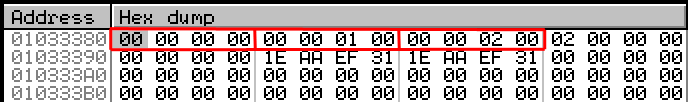
\includegraphics[width=0.6\textwidth]{patterns/13_arrays/5_multidimensional/olly_2D_2.png}
\caption{\olly: array is filled}
\end{figure}


\subsubsection{Access two-dimensional array as one-dimensional}

We can be easily assured that it's possible to access a two-dimensional array as one-dimensional array in at least two ways:

\lstinputlisting[style=customc]{patterns/13_arrays/5_multidimensional/2D_as_1D_EN.c}

Compile and run it: it shows correct values.

What MSVC 2013 did is fascinating, all three routines are just the same!

\lstinputlisting[caption=\Optimizing MSVC 2013 x64,style=customasmx86]{patterns/13_arrays/5_multidimensional/2D_as_1D_MSVC_2013_Ox_x64_EN.asm}

GCC also generates equivalent routines, but slightly different:

\lstinputlisting[caption=\Optimizing GCC 4.9 x64,style=customasmx86]{patterns/13_arrays/5_multidimensional/2D_as_1D_GCC49_x64_O3_EN.s}


\subsubsection{Three-dimensional array example}

It's the same for multidimensional arrays.

Now we are going to work with an array of type \Tint: each element requires 4 bytes in memory.

Let's see:

\lstinputlisting[caption=simple example,style=customc]{patterns/13_arrays/5_multidimensional/multi.c}

\myparagraph{x86}

We get (MSVC 2010):

\lstinputlisting[caption=MSVC 2010,style=customasmx86]{patterns/13_arrays/5_multidimensional/multi_msvc_EN.asm}

Nothing special. For index calculation, three input arguments are used 
in the formula $address=600 \cdot 4 \cdot x + 30 \cdot 4 \cdot y + 4z$, to represent the array as multidimensional.
Do not forget that the \Tint type is 32-bit (4 bytes),
so all coefficients must be multiplied by 4.

\lstinputlisting[caption=GCC 4.4.1,style=customasmx86]{patterns/13_arrays/5_multidimensional/multi_gcc_EN.asm}

The GCC compiler does it differently.

For one of the operations in the calculation ($30y$), GCC produces code without multiplication instructions.
This is how it done: 
$(y+y) \ll 4 - (y+y) = (2y) \ll 4 - 2y = 2 \cdot 16 \cdot y - 2y = 32y - 2y = 30y$. 
Thus, for the $30y$ calculation, only one addition operation,
one bitwise shift operation and one subtraction operation are used.
This works faster.

\myparagraph{ARM + \NonOptimizingXcodeIV (\ThumbMode)}

\lstinputlisting[caption=\NonOptimizingXcodeIV (\ThumbMode),style=customasmARM]{patterns/13_arrays/5_multidimensional/multi_Xcode_thumb_O0_EN.asm}

\NonOptimizing LLVM saves all variables in local stack, which is redundant.

The address of the array element is calculated by the formula we already saw.

\myparagraph{ARM + \OptimizingXcodeIV (\ThumbMode)}

\lstinputlisting[caption=\OptimizingXcodeIV (\ThumbMode),style=customasmARM]{patterns/13_arrays/5_multidimensional/multi_Xcode_thumb_O3_EN.asm}

The tricks for replacing multiplication by shift, addition and subtraction which we already saw
are also present here.

\myindex{ARM!\Instructions!RSB}
\myindex{ARM!\Instructions!SUB}
Here we also see a new instruction for us: \RSB (\IT{Reverse Subtract}).

It works just as \SUB, but it swaps its operands with each other before execution.
Why?
\myindex{ARM!Optional operators!LSL}
\SUB and \RSB  are instructions, to the second operand of which shift coefficient may be applied: (\INS{LSL\#4}). 

But this coefficient can be applied only to second operand.

That's fine for commutative operations like addition or multiplication 
(operands may be swapped there without changing the result).

But subtraction is a non-commutative operation, so \RSB exist for these cases.

\myparagraph{MIPS}

\myindex{MIPS!Global Pointer}
My example is tiny, so the GCC compiler decided to put the $a$ array into the 64KiB area 
addressable by the Global Pointer.

\lstinputlisting[caption=\Optimizing GCC 4.4.5 (IDA),style=customasmMIPS]{patterns/13_arrays/5_multidimensional/multi_MIPS_O3_IDA_EN.lst}



\subsubsection{More examples}

The computer screen is represented as a 2D array, but the video-buffer is a linear 1D array. 
We talk about it here: \myref{Mandelbrot_demo}.

Another example in this book is Minesweeper game: it's field is also two-dimensional array: \ref{minesweeper_winxp}.

}
\RU{\subsection{Многомерные массивы}

Внутри многомерный массив выглядит так же как и линейный.

Ведь память компьютера линейная, это одномерный массив.
Но для удобства этот одномерный массив легко представить как многомерный.

К примеру, вот как элементы массива 3x4 расположены в одномерном массиве из 12 ячеек:

% TODO FIXME not clear. First, horizontal would be better. Second, why two columns?
% I'd first show 3x4 with numbered elements (e.g. 32-bit ints) in colored lines,
% then linear with the same numbered elements (and colored blocks)
% then linear with addresses (offsets) - assuming let say 32-bit ints.
\begin{table}[H]
\centering
\begin{tabular}{ | l | l | }
\hline
Смещение в памяти & элемент массива \\
\hline
0 & [0][0] \\
\hline
1 & [0][1] \\
\hline
2 & [0][2] \\
\hline
3 & [0][3] \\
\hline
4 & [1][0] \\
\hline
5 & [1][1] \\
\hline
6 & [1][2] \\
\hline
7 & [1][3] \\
\hline
8 & [2][0] \\
\hline
9 & [2][1] \\
\hline
10 & [2][2] \\
\hline
11 & [2][3] \\
\hline
\end{tabular}
\caption{Двухмерный массив представляется в памяти как одномерный}
\end{table}

Вот по каким адресам в памяти располагается каждая ячейка двухмерного массива 3*4:

\begin{table}[H]
\centering
\begin{tabular}{ | l | l | l | l | }
\hline                        
0 & 1 & 2 & 3 \\
\hline  
4 & 5 & 6 & 7 \\
\hline  
8 & 9 & 10 & 11 \\
\hline  
\end{tabular}
\caption{Адреса в памяти каждой ячейки двухмерного массива}
\end{table}

\myindex{row-major order}
Чтобы вычислить адрес нужного элемента, сначала умножаем первый индекс (строку) на 4 (ширину массива), 
затем прибавляем второй индекс (столбец).

Это называется \IT{row-major order}, 
и такой способ представления массивов и матриц используется по крайней мере в \CCpp и Python. 
Термин \IT{row-major order} означает по-русски примерно следующее: \q{сначала записываем элементы первой строки, затем второй,~\dots~и~элементы последней 
строки в самом конце}.

\myindex{column-major order}
\myindex{Фортран}
Другой способ представления называется \IT{column-major order} (индексы массива используются в обратном порядке) 
и это используется по крайней мере в Фортране, MATLAB и R. 
Термин \IT{column-major order} означает по-русски
следующее: \q{сначала записываем элементы первого столбца, затем второго,~\dots~и~элементы последнего столбца
в самом конце}.

Какой из способов лучше?
В терминах производительности и кэш-памяти, лучший метод организации данных это тот,
при котором к данным обращаются последовательно.

Так что если ваша функция обращается к данным построчно, то \IT{row-major order} лучше,
и наоборот.

% subsections
\subsubsection{Пример с двумерным массивов}

Мы будем работать с массивом типа \Tchar. Это значит, что каждый элемент требует
только одного байта в памяти.

\myparagraph{Пример с заполнением строки}
\myindex{\olly}

Заполняем вторую строку значениями 0..3:

\lstinputlisting[caption=Пример с заполнением строки,style=customc]{patterns/13_arrays/5_multidimensional/two1_RU.c}

Все три строки обведены красным. 
Видно, что во второй теперь имеются байты 0, 1, 2 и 3:

\begin{figure}[H]
\centering
\includegraphics[width=0.6\textwidth]{patterns/13_arrays/5_multidimensional/olly_2D_1.png}
\caption{\olly: массив заполнен}
\end{figure}

\myparagraph{Пример с заполнением столбца}
\myindex{\olly}

Заполняем третий столбец значениями 0..2:

\lstinputlisting[caption=Пример с заполнением столбца,style=customc]{patterns/13_arrays/5_multidimensional/two2_RU.c}

Здесь также обведены красным три строки. 
Видно, что в каждой строке, на третьей позиции, теперь записаны 0, 1 и 2.

\begin{figure}[H]
\centering
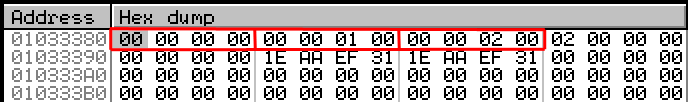
\includegraphics[width=0.6\textwidth]{patterns/13_arrays/5_multidimensional/olly_2D_2.png}
\caption{\olly: массив заполнен}
\end{figure}

\subsubsection{Работа с двухмерным массивом как с одномерным}

Мы можем легко убедиться, что можно работать с двухмерным массивом как с одномерным,
используя по крайней мере два метода:

\lstinputlisting[style=customc]{patterns/13_arrays/5_multidimensional/2D_as_1D_RU.c}

Компилируете и запускаете: мы увидим корректные значения.

Очарователен результат работы MSVC 2013~--- все три процедуры одинаковые!

\lstinputlisting[caption=\Optimizing MSVC 2013 x64,style=customasmx86]{patterns/13_arrays/5_multidimensional/2D_as_1D_MSVC_2013_Ox_x64_RU.asm}

GCC сгенерировал практически одинаковые процедуры:

\lstinputlisting[caption=\Optimizing GCC 4.9 x64,style=customasmx86]{patterns/13_arrays/5_multidimensional/2D_as_1D_GCC49_x64_O3_RU.s}


\subsubsection{Пример с трехмерным массивом}

То же самое и для многомерных массивов.
На этот раз будем работать с массивом типа \Tint: каждый элемент требует 4 байта в памяти.

Попробуем:

\lstinputlisting[caption=простой пример,style=customc]{patterns/13_arrays/5_multidimensional/multi.c}

\myparagraph{x86}

В итоге (MSVC 2010):

\lstinputlisting[caption=MSVC 2010,style=customasmx86]{patterns/13_arrays/5_multidimensional/multi_msvc_RU.asm}

В принципе, ничего удивительного. В \TT{insert()} для вычисления адреса нужного элемента массива 
три входных аргумента перемножаются по формуле $address=600 \cdot 4 \cdot x + 30 \cdot 4 \cdot y + 4z$, 
чтобы представить массив трехмерным.
Не забывайте также, что тип \Tint 32-битный (4 байта), поэтому все коэффициенты нужно умножить на 4.

\lstinputlisting[caption=GCC 4.4.1,style=customasmx86]{patterns/13_arrays/5_multidimensional/multi_gcc_RU.asm}

Компилятор GCC решил всё сделать немного иначе.
Для вычисления одной из операций ($30y$), GCC создал код, где нет самой операции умножения.

Происходит это так: 
$(y+y) \ll 4 - (y+y) = (2y) \ll 4 - 2y = 2 \cdot 16 \cdot y - 2y = 32y - 2y = 30y$. 
Таким образом, для вычисления $30y$ используется только операция сложения, 
операция битового сдвига и операция вычитания.
Это работает быстрее.

\myparagraph{ARM + \NonOptimizingXcodeIV (\ThumbMode)}

\lstinputlisting[caption=\NonOptimizingXcodeIV (\ThumbMode),style=customasmARM]{patterns/13_arrays/5_multidimensional/multi_Xcode_thumb_O0_RU.asm}

\NonOptimizing LLVM сохраняет все переменные в локальном стеке, хотя это и избыточно.

Адрес элемента массива вычисляется по уже рассмотренной формуле.

\myparagraph{ARM + \OptimizingXcodeIV (\ThumbMode)}

\lstinputlisting[caption=\OptimizingXcodeIV (\ThumbMode),style=customasmARM]{patterns/13_arrays/5_multidimensional/multi_Xcode_thumb_O3_RU.asm}

Тут используются уже описанные трюки для замены умножения на операции сдвига, сложения и вычитания.

\myindex{ARM!\Instructions!RSB}
\myindex{ARM!\Instructions!SUB}
Также мы видим новую для себя инструкцию \RSB (\IT{Reverse Subtract}).
Она работает так же, как и \SUB, только меняет операнды местами.

Зачем?
\myindex{ARM!Optional operators!LSL}
\SUB и \RSB это те инструкции, ко второму операнду которых можно применить коэффициент сдвига, как мы видим и здесь: (\INS{LSL\#4}). 
Но этот коэффициент можно применить только ко второму операнду.

Для коммутативных операций, таких как сложение или умножение, 
операнды можно менять местами и это не влияет на результат.

Но вычитание~--- операция некоммутативная, так что для этих случаев существует инструкция \RSB.

\myparagraph{MIPS}

\myindex{MIPS!Global Pointer}

Мой пример такой крошечный, что компилятор GCC решил разместить массив $a$ в 64KiB-области,
адресуемой при помощи Global Pointer.

\lstinputlisting[caption=\Optimizing GCC 4.4.5 (IDA),style=customasmMIPS]{patterns/13_arrays/5_multidimensional/multi_MIPS_O3_IDA_RU.lst}



\subsubsection{Ещё примеры}

Компьютерный экран представляет собой двумерный массив, но видеобуфер это линейный
одномерный массив. 
Мы рассматриваем это здесь: \myref{Mandelbrot_demo}.

Еще один пример в этой книге это игра ``Сапер'': её поле это тоже двухмерный массив: \ref{minesweeper_winxp}.

}
\DE{\subsection{Multidimensionale Arrays}
Intern ist ein multidimensionales Array im Prinzip das gleiche wie ein lineares Array.

Da der Speicher eines Rechners linear ist, ist es ein eindimensionales Array.
Zur Vereinfachung kann dieses multidimensionales Array leicht als eindimensional dargestellt werden.

Beispielsweise werden die Elemente eines 3x4 Arrays folgendermaßen in einem eindimensionalen Array aus 12 Zellen
gespeichert:

% TODO FIXME not clear. First, horizontal would be better. Second, why two columns?
% I'd first show 3x4 with numbered elements (e.g. 32-bit ints) in colored lines,
% then linear with the same numbered elements (and colored blocks)
% then linear with addresses (offsets) - assuming let say 32-bit ints.
\begin{table}[H]
\centering
\begin{tabular}{ | l | l | }
\hline
Offset im Speicher & Arrayelement \\
\hline
0 & [0][0] \\
\hline
1 & [0][1] \\
\hline
2 & [0][2] \\
\hline
3 & [0][3] \\
\hline
4 & [1][0] \\
\hline
5 & [1][1] \\
\hline
6 & [1][2] \\
\hline
7 & [1][3] \\
\hline
8 & [2][0] \\
\hline
9 & [2][1] \\
\hline
10 & [2][2] \\
\hline
11 & [2][3] \\
\hline
\end{tabular}
\caption{Zweidimensionales Array in eindimensionaler Speicherdarstellung}
\end{table}

Auf diese Weise wird jede Zellen des 3*4 Arrays im Speicher abgelegt:

% TODO coordinates. TikZ?
\begin{table}[H]
\centering
\begin{tabular}{ | l | l | l | l | }
\hline                        
0 & 1 & 2 & 3 \\
\hline  
4 & 5 & 6 & 7 \\
\hline  
8 & 9 & 10 & 11 \\
\hline  
\end{tabular}
\caption{Speicheradressen jeder Zelle des zweidimensionalen Arrays}
\end{table}

\myindex{row-major order}
Um also die Adresse des benötigten Elements zu berechnen, multiplizieren wir zunächst den ersten Index mit 4 (der
Arraybreite) und addieren dann den zweiten Index.
Dies nennt man \IT{Zeilenordnung} (engl. row-major order) und diese Methode zur Darstellung von Arrays und Matrizen
wird mindestens von \CCpp und Python verwendet.
Der Ausdruck row-major order bedeutet: \q{schreibe zuerst die Elemente der ersten Zeilen, dann die zweite Zeile\dots
und schließlich die Elemente der letzten Zeile}.

\myindex{column-major order}
\myindex{Fortran}
Eine andere Methode zur Darstellung heißt \IT{Spaltenordnung} (engl. column-major order) (die Indizes des Arrays werden
in umgekehrter Reihenfolge verwendet) und wird zumindest in Fortran, MATLAB und R verwendet.
Der Ausdruck column-major oder bedeutet: \q{schreibe zuerst die Elemente der ersten Spalte, dann die zweite Spalte\dots
und schließlich die Elemente der letzten Spalte}.

Welche Method ist besser?

Generel ist hinsichtlich Performance und Cachespeicher die beste Methode der Datenorganisation diejenige, in der auf die
Elemente sequentiell zugegriffen wird.

Wenn eine Funktion auf Daten zeilenweise zugreift, ist Zeilenordnung besser und umgekehrt.

% subsections
\subsubsection{Beispiel für zweidimensionales Array}
Wir werden mit einem Array vom Typ \Tchar arbeiten, was bedeutet, dass jedes Element nur ein Byte Speicherplatz
benötigt.


\myparagraph{Beispiel: Zeile füllen}
\myindex{\olly}
Füllen wir die zweite Zeilen mit den Werten 0..3:

\lstinputlisting[caption=Row filling example,style=customc]{patterns/13_arrays/5_multidimensional/two1_DE.c}
Alle drei Zeilen sind rot markiert.
Wir erkennen, dass die zweite Zeilen nun die Werte 0,1,2 und 3 enthält:

\begin{figure}[H]
\centering
\includegraphics[width=0.6\textwidth]{patterns/13_arrays/5_multidimensional/olly_2D_1.png}
\caption{\olly: Array ist befüllt}
\end{figure}

\myparagraph{Beipsiel: Spalte füllen}
\myindex{\olly}
Füllen wir die dritte Spalte mit den Werten 0..2:

\lstinputlisting[caption=Column filling example,style=customc]{patterns/13_arrays/5_multidimensional/two2_DE.c}

Die drei Spalten sind hier ebenfalls rot markiert.

Wir erkennen, dass sich in jeder Zeile an der dritten Stelle die Werte 0,1 und 2 befinden. 

\begin{figure}[H]
\centering
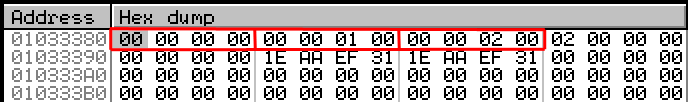
\includegraphics[width=0.6\textwidth]{patterns/13_arrays/5_multidimensional/olly_2D_2.png}
\caption{\olly: Array ist befüllt}
\end{figure}


\subsubsection{Eindimensionaler Zugriff auf zweidimensionales Array}
Wir können uns leicht davon überzeugen, dass es auf mindestens zwei Arten möglich ist, auf ein zweidimensionales Array
eindimensional zuzugreifen:

\lstinputlisting[style=customc]{patterns/13_arrays/5_multidimensional/2D_as_1D_DE.c}

Kompilieren und ausführen: es zeigt korrekte Werte an
Was MSVC 2013 getan hat ist faszinierend: alle drei Routinen sind identisch!

\lstinputlisting[caption=\Optimizing MSVC 2013 x64,style=customasmx86]{patterns/13_arrays/5_multidimensional/2D_as_1D_MSVC_2013_Ox_x64_EN.asm}

GCC erzeugt ebenfalls äquivalente Routinen, aber ein wenig anders:

\lstinputlisting[caption=\Optimizing GCC 4.9 x64,style=customasmx86]{patterns/13_arrays/5_multidimensional/2D_as_1D_GCC49_x64_O3_EN.s}


\subsubsection{Beispiel: dreidimensionales Array}

Mit multidimensionalen Arrays ist es das gleiche.

Wir werden nun mit einem Array vom Typ \Tint arbeiten: jedes Element benötigt 4 Byte Speicherplatz.

Sehen wir es uns an:

\lstinputlisting[caption=simple example,style=customc]{patterns/13_arrays/5_multidimensional/multi.c}

\myparagraph{x86}

Wir erhalten das Folgende (MSVC 2010):

\lstinputlisting[caption=MSVC 2010,style=customasmx86]{patterns/13_arrays/5_multidimensional/multi_msvc_DE.asm}
Nichts Außergewöhnliches. Zur Berechnung des Index' werden in der Formel $address=600 \cdot 4 \cdot x + 30 \cdot 4 \cdot
y + 4z$ drei Eingabewerte verwendet, um das multidimensionale Array zu repräsentieren.
Vergessen wir nicht, dass der \Tint Typ 32 Bit (4 Byte) breit ist, sodass alle Koeffizienten mit 4 multipliziert werden
müssen.

\lstinputlisting[caption=GCC 4.4.1,style=customasmx86]{patterns/13_arrays/5_multidimensional/multi_gcc_DE.asm}
Der GCC Compiler arbeitet anders.

Für eine der Operationen in der Berechnung ($30y$) produziet GCC Code ohne Multiplikationsbefehle.
Das funktioniert wie folgt:
$(y+y) \ll 4 - (y+y) = (2y) \ll 4 - 2y = 2 \cdot 16 \cdot y - 2y = 32y - 2y = 30y$.

So werden für die $30y$ Berechnung nur ein Addierbefehl, eine bitweiser Verschiebebefehl und ein Subtraktionsbefehl
verwendet. So geht es schneller.

\myparagraph{ARM + \NonOptimizingXcodeIV (\ThumbMode)}

\lstinputlisting[caption=\NonOptimizingXcodeIV
(\ThumbMode),style=customasmARM]{patterns/13_arrays/5_multidimensional/multi_Xcode_thumb_O0_DE.asm}

\NonOptimizing LLVM speichert alle Variablen auf dem lokalen Stack, was redundant ist.

Die Adresse des Arrayelements wird über die eben gezeigte Formel berechnet.

\myparagraph{ARM + \OptimizingXcodeIV (\ThumbMode)}

\lstinputlisting[caption=\OptimizingXcodeIV
(\ThumbMode),style=customasmARM]{patterns/13_arrays/5_multidimensional/multi_Xcode_thumb_O3_DE.asm}
Die Tricks für das Ersetzen der Multiplikation durch Verschieben, Addieren und Subtrahieren, die wir bereits
kennengelernt haben, kommen hier auch vor.

\myindex{ARM!\Instructions!RSB}
\myindex{ARM!\Instructions!SUB}
Hier finden wir auch einen für uns neuen Befehl: \RSB (\IT{Reverse Subtract}).

Er arbeitet genau wie \SUB, aber vertauscht die Operanden vor der Ausführung. Warum?

\myindex{ARM!Optional operators!LSL}
\SUB und \RSB  sind Befehle, bei denen auf den zweiten Operanden eine bitweise Verschiebung angewendet werden kann:
(\INS{LSL\#4}).
Dieser Koeffizient kann aber nur auf den zweiten Operanden angewendet werden.

Das ist günstig für kommutative Operationen wie Addition und Multiplikation (die Operanden können vertauscht werden,
ohne das Ergebnis zu verändern).

Subtraktion dagegen ist nicht kommutativ, weshalb für diese Fälle \RSB existiert.

\myparagraph{MIPS}

\myindex{MIPS!Global Pointer}
Das Beispiel ist sehr klein, sodass der GCC Compiler entschieden hat das Array $a$ im 64KiB Platz abzulegen, um es durch
den globalen Pointer zugreifbar zu machen.

\lstinputlisting[caption=\Optimizing GCC 4.4.5
(IDA),style=customasmMIPS]{patterns/13_arrays/5_multidimensional/multi_MIPS_O3_IDA_DE.lst}



\subsubsection{Weitere Beispiele}
Der Bildschirm wird als 2D-Array dargestellt, aber der Videopuffer ist ein lineares 1D-Array.
Wir betrachten hier näher: \myref{Mandelbrot_demo}.

Ein anderes Beispiel in diesem Buch ist das Spiel Minesweeper: das Feld ist auch ein zweidimensionales Array:
\ref{minesweeper_winxp}.

}

\EN{\subsection{Pack of strings as a two-dimensional array}

Let's revisit the function that returns the name of a month: \lstref{get_month1}.

As you see, at least one memory load operation is needed to prepare a pointer to the string
that's the month's name.

Is it possible to get rid of this memory load operation?

In fact yes, if you represent the list of strings as a two-dimensional array:

\lstinputlisting[style=customc]{patterns/13_arrays/55_month_2D/month2_EN.c}

Here is what we've get:

\lstinputlisting[caption=\Optimizing MSVC 2013 x64,style=customasmx86]{patterns/13_arrays/55_month_2D/MSVC2013_x64_Ox_EN.asm}

There are no memory accesses at all.

All this function does is to calculate a point at which the first character of the name of the month is: 
$pointer\_to\_the\_table + month * 10$.

There are also two \LEA instructions, which effectively work as several \MUL and \MOV instructions.

The width of the array is 10 bytes. 

Indeed, the longest string here---\q{September}---is 9 bytes, and plus the terminating zero is 10 bytes.

The rest of the month names are padded by zero bytes, so they all occupy the same space (10 bytes).

Thus, our function works even faster, because all string start at an address which can be
calculated easily.

\Optimizing GCC 4.9 can do it even shorter:

\begin{lstlisting}[caption=\Optimizing GCC 4.9 x64,style=customasmx86]
	movsx	rdi, edi
	lea	rax, [rdi+rdi*4]
	lea	rax, month2[rax+rax]
	ret
\end{lstlisting}

\LEA is also used here for multiplication by 10.

Non-optimizing compilers do multiplication differently.

\lstinputlisting[caption=\NonOptimizing GCC 4.9 x64,style=customasmx86]{patterns/13_arrays/55_month_2D/x64_GCC49_O0_EN.asm}

\NonOptimizing MSVC just uses \IMUL instruction:
\myindex{x86!\Instructions!IMUL}

\lstinputlisting[caption=\NonOptimizing MSVC 2013 x64,style=customasmx86]{patterns/13_arrays/55_month_2D/MSVC2013_x64_EN.asm}

\myindex{\CompilerAnomaly}
\label{MSVC2013_anomaly}

But one thing is weird here: why add multiplication by zero and adding zero to the final result?

This looks like a compiler code generator quirk, which wasn't caught by the compiler's tests
(the resulting code works correctly, after all).
% класс!
%
We intentionally consider such pieces of code so the reader would understand, 
that sometimes one shouldn't puzzle over such compiler artifacts.

\subsubsection{32-bit ARM}

\Optimizing Keil 
for Thumb mode uses the multiplication instruction \INS{MULS}:

\lstinputlisting[caption=\OptimizingKeilVI (\ThumbMode),style=customasmARM]{patterns/13_arrays/55_month_2D/Keil_O3_thumb_EN.asm}

\Optimizing Keil for ARM mode uses add and shift operations:

\lstinputlisting[caption=\OptimizingKeilVI (\ARMMode),style=customasmARM]{patterns/13_arrays/55_month_2D/Keil_O3_ARM_EN.asm}

\subsubsection{ARM64}

\lstinputlisting[caption=\Optimizing GCC 4.9 ARM64,style=customasmARM]{patterns/13_arrays/55_month_2D/GCC49_ARM64_EN.asm}

\myindex{ARM!\Instructions!SXTW}
\myindex{ARM!\Instructions!ADRP/ADD pair}

\INS{SXTW} is used for sign-extension and promoting input 32-bit value into a 64-bit one and storing it in X0.

\ADRP/\ADD pair is used for loading the address of the table.

The \ADD instructions also has a \LSL suffix, which helps with multiplications.

\subsubsection{MIPS}
\lstinputlisting[caption=\Optimizing GCC 4.4.5 (IDA),style=customasmMIPS]{patterns/13_arrays/55_month_2D/MIPS_O3_IDA_EN.lst}

\subsubsection{\Conclusion{}}

This is a bit old-school technique to store text strings.
You may find a lot of it in \oracle, for example.
It's hard to say if it's worth doing on modern computers.
Nevertheless, it is a good example of arrays, so it was added to this book.

}
\RU{\subsection{Набор строк как двухмерный массив}

Снова вернемся к примеру, который возвращает название месяца: \lstref{get_month1}.
Как видно, нужна как минимум одна операция загрузки из памяти для подготовки указателя на строку,
состоящую из имени месяца.

Возможно ли избавиться от операции загрузки из памяти?

Да, если представить список строк как двумерный массив:

\lstinputlisting[style=customc]{patterns/13_arrays/55_month_2D/month2_RU.c}

Вот что получаем:

\lstinputlisting[caption=\Optimizing MSVC 2013 x64,style=customasmx86]{patterns/13_arrays/55_month_2D/MSVC2013_x64_Ox_RU.asm}

Здесь нет обращений к памяти вообще.
Эта функция только вычисляет место, где находится первый символ названия месяца:
 
$pointer\_to\_the\_table + month * 10$.
Там также две инструкции \LEA, которые работают как несколько инструкций \MUL и \MOV.

Ширина массива~--- 10 байт. 
Действительно, самая длинная строка это \q{September} (9 байт) плюс оконечивающий ноль, получается 10 байт.

Остальные названия месяцев дополнены нулевыми байтами, чтобы они занимали столько же места (10 байт).

Таким образом, наша функция и работает быстрее, потому что все строки начинаются с тех адресов, 
которые легко вычислить.

\Optimizing GCC 4.9 может ещё короче:

\begin{lstlisting}[caption=\Optimizing GCC 4.9 x64,style=customasmx86]
	movsx	rdi, edi
	lea	rax, [rdi+rdi*4]
	lea	rax, month2[rax+rax]
	ret
\end{lstlisting}

\LEA здесь также используется для умножения на 10.

Неоптимизирующие компиляторы делают умножение по-разному.

\lstinputlisting[caption=\NonOptimizing GCC 4.9 x64,style=customasmx86]{patterns/13_arrays/55_month_2D/x64_GCC49_O0_RU.asm}

\NonOptimizing MSVC просто использует инструкцию \IMUL:
\myindex{x86!\Instructions!IMUL}

\lstinputlisting[caption=\NonOptimizing MSVC 2013 x64,style=customasmx86]{patterns/13_arrays/55_month_2D/MSVC2013_x64_RU.asm}

\myindex{\CompilerAnomaly}
\label{MSVC2013_anomaly}
Но вот что странно: зачем добавлять умножение на ноль и добавлять ноль к конечному результату?

Это выглядит как странность кодегенератора компилятора, который не был покрыт тестами
компилятора. Но так или иначе, итоговый код работает корректно.
% класс! ЩИТО?
Мы сознательно рассматриваем такие фрагменты кода, чтобы читатель понимал, что иногда не нужно
ломать себе голову над подобными артефактами компиляторов.

\subsubsection{32-bit ARM}

\Optimizing Keil для режима Thumb использует инструкцию умножения \INS{MULS}:

\lstinputlisting[caption=\OptimizingKeilVI (\ThumbMode),style=customasmARM]{patterns/13_arrays/55_month_2D/Keil_O3_thumb_RU.asm}

\Optimizing Keil для режима ARM использует операции сложения и сдвига:

\lstinputlisting[caption=\OptimizingKeilVI (\ARMMode),style=customasmARM]{patterns/13_arrays/55_month_2D/Keil_O3_ARM_RU.asm}

\subsubsection{ARM64}

\lstinputlisting[caption=\Optimizing GCC 4.9 ARM64,style=customasmARM]{patterns/13_arrays/55_month_2D/GCC49_ARM64_RU.asm}

\myindex{ARM!\Instructions!SXTW}
\myindex{ARM!\Instructions!ADRP/ADD pair}
\INS{SXTW} используется для знакового расширения и расширения
входного 32-битного значения в 64-битное и сохранения его в X0.

Пара \ADRP/\ADD используется для загрузки адреса таблицы.

У инструкции \ADD также есть суффикс \LSL, что помогает с умножением.

\subsubsection{MIPS}
\lstinputlisting[caption=\Optimizing GCC 4.4.5 (IDA),style=customasmMIPS]{patterns/13_arrays/55_month_2D/MIPS_O3_IDA_RU.lst}

\subsubsection{\Conclusion{}}

Это немного олд-скульная техника для хранения текстовых строк.
Много такого можно найти в \oracle, например.
Трудно сказать, стоит ли оно того на современных компьютерах.
Так или иначе, это был хороший пример массивов, поэтому он был добавлен в эту книгу.

}
\DE{\subsection{Strings als zweidimensionales Array}
Betrachten wir erneut die Funktion, die den Namen eines Monats zurückgibt: \lstref{get_month1}.

Wie man sieht wird mindestens eine Befehl benötigt, der einen Wert aus dem Speicher lädt, um den Pointer auf den String,
der den Monatsnamen enthält, vorzubereiten.

Ist es möglich diesen Speicherzugriff loszuwerden?

Die Antwort ist: ja, wenn man die Liste aus String als zweidimensionales Array darstellt:

\lstinputlisting[style=customc]{patterns/13_arrays/55_month_2D/month2_DE.c}

Hier ist was wir erhalten:

\lstinputlisting[caption=\Optimizing MSVC 2013
x64,style=customasmx86]{patterns/13_arrays/55_month_2D/MSVC2013_x64_Ox_DE.asm}

Es gibt überhaupt keine Speicherzugriffe.
Alles, was diese Funktion tut, ist einen Pointer zu berechnen, der auf den ersten Buchstaben des Monats
zeigt:$pointer\_to\_the\_table + month \cdot 10$.

Es gibt auch zwei \LEA Befehle, die wie mehrere \MUL und \MOV Befehle funktionieren.

Die Breite des Arrays beträgt 10 Byte.

Der längste String im Beispiel---\q{September}---hat eine Länge von 9 Byte zuzüglich einer terminierenden Null, also
insgesamt 10 Byte.

Die übrigen Monatsnamen werden mit Zerobytes aufgefüllt, sodass alle denselben Speicherplatz (10 Byte) benötigen.

Dadurch arbeitet unsere Funktion noch schneller, denn die Startadresse jedes Strings kann so einfach berechnet werden.

\Optimizing GCC 4.9 kann sogar noch kürzeren Code erzeugen:

\begin{lstlisting}[caption=\Optimizing GCC 4.9 x64,style=customasmx86]
	movsx	rdi, edi
	lea	rax, [rdi+rdi*4]
	lea	rax, month2[rax+rax]
	ret
\end{lstlisting}

\LEA wird hier auch für die Multiplikation mit 10 verwendet.

Nicht optimierende Compiler führen die Multiplikation anders durch.

\lstinputlisting[caption=\NonOptimizing GCC 4.9
x64,style=customasmx86]{patterns/13_arrays/55_month_2D/x64_GCC49_O0_DE.asm}

\NonOptimizing MSVC verwendet nur den \IMUL Befehl:
\myindex{x86!\Instructions!IMUL}

\lstinputlisting[caption=\NonOptimizing MSVC 2013
x64,style=customasmx86]{patterns/13_arrays/55_month_2D/MSVC2013_x64_DE.asm}

\myindex{\CompilerAnomaly}
\label{MSVC2013_anomaly}
Eine Sache hier ist seltsam: warum wird die Multiplikation mit null und die Addition von null zum Endergebnis
hinzugefügt?

Dies sieht wie ein Fehler im Codegenerator des Compilers aus, der nicht durch die Tests des Compilers abgefangen wurde.
(Trotzdem funktioniert der erzeugte Code korrekt.)

% класс!
%
Wir betrachten solche Codes ganz bewußt, damit der Leser sich klarmacht, dass man sich über solche Merkwürdigkeiten und
Artefakte des Compilers nicht allzu sehr wundern soll.

\subsubsection{32-bit ARM}

\Optimizing Keil im Thumb mode verwendet zur Multiplikation den Befehl \INS{MULS}:

\lstinputlisting[caption=\OptimizingKeilVI
(\ThumbMode),style=customasmARM]{patterns/13_arrays/55_month_2D/Keil_O3_thumb_DE.asm}

\Optimizing Keil für ARM mode verwendet Additions- und Schiebebefehle:

\lstinputlisting[caption=\OptimizingKeilVI
(\ARMMode),style=customasmARM]{patterns/13_arrays/55_month_2D/Keil_O3_ARM_DE.asm}

\subsubsection{ARM64}

\lstinputlisting[caption=\Optimizing GCC 4.9
ARM64,style=customasmARM]{patterns/13_arrays/55_month_2D/GCC49_ARM64_DE.asm}

\myindex{ARM!\Instructions!SXTW}
\myindex{ARM!\Instructions!ADRP/ADD pair}
\INS{SXTW} wird für Vorzeichenerweiterung und Übertragung von 32-Bit-Werten in 64-Bit-Werte und das Speichern in X0
verwendet.

Das \ADRP/\ADD Paar wird für das Laden der Adresse der Tabelle verwendet.

Der \ADD Befehl trägt auch den \LSL Suffix, der bei der Multiplikation hilft.

\subsubsection{MIPS}
\lstinputlisting[caption=\Optimizing GCC 4.4.5 (IDA),style=customasmMIPS]{patterns/13_arrays/55_month_2D/MIPS_O3_IDA_EN.lst}

\subsubsection{\Conclusion{}}
Das Gezeigte ist eine etwas altmodische Technik um Textstrings zu speichern.
Man findet diesen Ansatz beispielsweise oft in \oracle.
Es ist schwer zu sagen, ob es sich für moderne Computer lohnt.
Nichtsdestotrotz ist es ein gutes Beispiel für Arrays und hat daher seine Berechtigung in diesem Buch.

}

\EN{\subsection{\Conclusion{}}

An array is a pack of values in memory located adjacently.

It's true for any element type, including structures.

Access to a specific array element is just a calculation of its address.
}
\RU{\subsection{\Conclusion{}}

Массив это просто набор значений в памяти, расположенных рядом друг с другом.

Это справедливо для любых типов элементов, включая структуры.

Доступ к определенному элементу массива это просто вычисление его адреса.

}
\DE{\subsection{\Conclusion{}}

Ein Array ist eine Ansammlung von Werten, die im Speicher nebeneinander angeordnet sind.

Dies gilt für alle Elementtypen und sogar für Structs.

Der Zugriff auf ein spezielles Element des Arrays entspricht lediglich eine Berechnung von dessen Adresse.}

\myindex{Hex-Rays}

\RU{\section{Кстати}
Итак, указатель на массив и адрес первого элемента --- это одно и то же.
Вот почему выражения \TT{ptr[0]} и \TT{*ptr} в \CCpp равноценны.
Любопытно что Hex-Rays часто заменяет первое вторым.
Он делает это в тех случаях, когда не знает, что имеет дело с указателем на целый массив,
и думает, что это указатель только на одну переменную.}%
\EN{\section{By the way}
So, pointer to an array and address of a first element---is the same thing.
This is why \TT{ptr[0]} and \TT{*ptr} expressions are equivalent in \CCpp.
It's interesting to note that Hex-Rays often replaces the first by the second.
It does so when it have no idea that it works with pointer to the whole array,
and thinks that this is a pointer to single variable.}
\DEph{}

\subsection{\Exercises}

\begin{itemize}
	\item \url{http://challenges.re/62}
	\item \url{http://challenges.re/63}
	\item \url{http://challenges.re/64}
	\item \url{http://challenges.re/65}
	\item \url{http://challenges.re/66}
\end{itemize}



\EN{\section{\BitfieldsChapter}
\label{sec:bitfields}

A lot of functions define their input arguments as flags in bit fields.
\myindex{\CLanguageElements!C99!bool}

Of course, they could be substituted by a set of \Tbool-typed variables, but it is not frugally.

% sections
\subsection{\RU{Проверка какого-либо бита}\EN{Specific bit checking}}

\EN{\input{patterns/14_bitfields/1_check/x86_EN}}
\RU{\input{patterns/14_bitfields/1_check/x86_RU}}
\EN{\input{patterns/14_bitfields/1_check/ARM_EN}}
\RU{\input{patterns/14_bitfields/1_check/ARM_RU}}


\subsection{\RU{Установка и сброс отдельного бита}\EN{Setting and clearing specific bits}}

\RU{Например}\EN{For example}:

\lstinputlisting[style=customc]{patterns/14_bitfields/2_set_reset/set_reset.c}

\EN{\input{patterns/14_bitfields/2_set_reset/x86_EN}}
\RU{\input{patterns/14_bitfields/2_set_reset/x86_RU}}
\EN{\input{patterns/14_bitfields/2_set_reset/ARM_EN}}
\RU{\input{patterns/14_bitfields/2_set_reset/ARM_RU}}
\EN{\input{patterns/14_bitfields/2_set_reset/MIPS_EN}}
\RU{\input{patterns/14_bitfields/2_set_reset/MIPS_RU}}


\EN{\input{patterns/14_bitfields/3_shifts/main_EN}}
\RU{\input{patterns/14_bitfields/3_shifts/main_RU}}


\EN{\input{patterns/14_bitfields/35_set_reset_FPU/main_EN}}
\RU{\input{patterns/14_bitfields/35_set_reset_FPU/main_RU}}

\EN{\input{patterns/14_bitfields/4_popcnt/main_EN}}
\RU{\input{patterns/14_bitfields/4_popcnt/main_RU}}


% TODO: add ROL/ROR
\subsection{\Conclusion{}}

\myindex{x86!\Instructions!SHR}
\myindex{x86!\Instructions!SHL}
\myindex{x86!\Instructions!SAR}

Analogous to the \CCpp shifting operators \TT{$\ll$} and \TT{$\gg$},
the shift instructions in x86 are \SHR/\SHL (for unsigned values) and \SAR/\SHL (for signed values).

\myindex{ARM!\Instructions!LSR}
\myindex{ARM!\Instructions!LSL}
\myindex{ARM!\Instructions!ASR}

The shift instructions in ARM are \LSR/\LSL (for unsigned values) and \ASR/\LSL (for signed values).

It's also possible to add shift suffix to some instructions 
(which are called \q{data processing instructions}).
% FIXME: which instructions?

\subsubsection{Check for specific bit (known at compile stage)}

Test if the 0b1000000 bit (0x40) is present in the register's value:

\lstinputlisting[caption=\CCpp,style=customc]{patterns/14_bitfields/c_snippet0.c}

\lstinputlisting[caption=x86,style=customasmx86]{patterns/14_bitfields/TEST_JNZ_EN.lst}

\lstinputlisting[caption=x86,style=customasmx86]{patterns/14_bitfields/TEST_JZ_EN.lst}

\lstinputlisting[caption=ARM (\ARMMode),style=customasmARM]{patterns/14_bitfields/TST_BNE_EN.lst}

\myindex{x86!\Instructions!AND}
\myindex{x86!\Instructions!TEST}

Sometimes, \AND is used instead of \TEST, but the flags that are set are the same.

\subsubsection{Check for specific bit (specified at runtime)}

This is usually done by this \CCpp code snippet (shift value by $n$ bits right, then cut off lowest bit):

\lstinputlisting[caption=\CCpp,style=customc]{patterns/14_bitfields/c_snippet1.c}

This is usually implemented in x86 code as:

\begin{lstlisting}[caption=x86,style=customasmx86]
; REG=input_value
; CL=n
SHR REG, CL
AND REG, 1
\end{lstlisting}

Or (shift 1 bit $n$ times left, isolate this bit in input value and check if it's not zero):

\lstinputlisting[caption=\CCpp,style=customc]{patterns/14_bitfields/c_snippet2.c}

This is usually implemented in x86 code as:

\begin{lstlisting}[caption=x86,style=customasmx86]
; CL=n
MOV REG, 1
SHL REG, CL
AND input_value, REG
\end{lstlisting}

\subsubsection{Set specific bit (known at compile stage)}

\begin{lstlisting}[caption=\CCpp]
value=value|0x40;
\end{lstlisting}

\begin{lstlisting}[caption=x86,style=customasmx86]
OR REG, 40h
\end{lstlisting}

\begin{lstlisting}[caption=ARM (\ARMMode) and ARM64,style=customasmARM]
ORR R0, R0, #0x40
\end{lstlisting}

\subsubsection{Set specific bit (specified at runtime)}

\lstinputlisting[caption=\CCpp,style=customc]{patterns/14_bitfields/c_snippet3.c}

This is usually implemented in x86 code as:

\begin{lstlisting}[caption=x86,style=customasmx86]
; CL=n
MOV REG, 1
SHL REG, CL
OR input_value, REG
\end{lstlisting}

\subsubsection{Clear specific bit (known at compile stage)}

Just apply \AND operation with the inverted value:

\begin{lstlisting}[caption=\CCpp,style=customc]
value=value&(~0x40);
\end{lstlisting}

\begin{lstlisting}[caption=x86,style=customasmx86]
AND REG, 0FFFFFFBFh
\end{lstlisting}

\begin{lstlisting}[caption=x64,style=customasmx86]
AND REG, 0FFFFFFFFFFFFFFBFh
\end{lstlisting}

This is actually leaving all bits set except one.

\myindex{ARM!\Instructions!BIC}

ARM in ARM mode has \BIC instruction, which works like the \NOT+\AND instruction pair:

\begin{lstlisting}[caption=ARM (\ARMMode),style=customasmARM]
BIC R0, R0, #0x40
\end{lstlisting}

\subsubsection{
Clear specific bit (specified at runtime)}

\lstinputlisting[caption=\CCpp,style=customc]{patterns/14_bitfields/c_snippet4.c}

\begin{lstlisting}[caption=x86,style=customasmx86]
; CL=n
MOV REG, 1
SHL REG, CL
NOT REG
AND input_value, REG
\end{lstlisting}

\subsection{\Exercises}

\begin{itemize}
	\item \url{http://challenges.re/67}
	\item \url{http://challenges.re/68}
	\item \url{http://challenges.re/69}
	\item \url{http://challenges.re/70}
\end{itemize}


}
\RU{\section{\BitfieldsChapter}
\label{sec:bitfields}

Немало функций задают различные флаги в аргументах при помощи битовых полей\footnote{bit fields в англоязычной литературе}.

\myindex{\CLanguageElements!C99!bool}
Наверное, вместо этого можно было бы использовать набор переменных типа \Tbool, но это было бы 
не очень экономно.

% sections
\subsection{\RU{Проверка какого-либо бита}\EN{Specific bit checking}}

\EN{\input{patterns/14_bitfields/1_check/x86_EN}}
\RU{\input{patterns/14_bitfields/1_check/x86_RU}}
\EN{\input{patterns/14_bitfields/1_check/ARM_EN}}
\RU{\input{patterns/14_bitfields/1_check/ARM_RU}}


\subsection{\RU{Установка и сброс отдельного бита}\EN{Setting and clearing specific bits}}

\RU{Например}\EN{For example}:

\lstinputlisting[style=customc]{patterns/14_bitfields/2_set_reset/set_reset.c}

\EN{\input{patterns/14_bitfields/2_set_reset/x86_EN}}
\RU{\input{patterns/14_bitfields/2_set_reset/x86_RU}}
\EN{\input{patterns/14_bitfields/2_set_reset/ARM_EN}}
\RU{\input{patterns/14_bitfields/2_set_reset/ARM_RU}}
\EN{\input{patterns/14_bitfields/2_set_reset/MIPS_EN}}
\RU{\input{patterns/14_bitfields/2_set_reset/MIPS_RU}}


\EN{\input{patterns/14_bitfields/3_shifts/main_EN}}
\RU{\input{patterns/14_bitfields/3_shifts/main_RU}}


\EN{\input{patterns/14_bitfields/35_set_reset_FPU/main_EN}}
\RU{\input{patterns/14_bitfields/35_set_reset_FPU/main_RU}}

\EN{\input{patterns/14_bitfields/4_popcnt/main_EN}}
\RU{\input{patterns/14_bitfields/4_popcnt/main_RU}}


% TODO: add ROL/ROR
\subsection{\Conclusion{}}

\myindex{x86!\Instructions!SHR}
\myindex{x86!\Instructions!SHL}
\myindex{x86!\Instructions!SAR}
Инструкции сдвига, аналогичные операторам \CCpp \TT{$\ll$} и \TT{$\gg$}, в x86 это \SHR/\SHL (для беззнаковых значений), \SAR/\SHL (для знаковых значений).

\myindex{ARM!\Instructions!LSR}
\myindex{ARM!\Instructions!LSL}
\myindex{ARM!\Instructions!ASR}
Инструкции сдвига в ARM это \LSR/\LSL (для беззнаковых значений), \ASR/\LSL (для знаковых значений).

Можно также добавлять суффикс сдвига для некоторых инструкций 
(которые называются \q{data processing instructions}).

% FIXME: which instructions?

\subsubsection{Проверка определенного бита (известного на стадии компиляции)}

Проверить, присутствует ли бит 0b1000000 (0x40) в значении в регистре:

\lstinputlisting[caption=\CCpp,style=customc]{patterns/14_bitfields/c_snippet0.c}

\lstinputlisting[caption=x86,style=customasmx86]{patterns/14_bitfields/TEST_JNZ_RU.lst}

\lstinputlisting[caption=x86,style=customasmx86]{patterns/14_bitfields/TEST_JZ_RU.lst}

\lstinputlisting[caption=ARM (\ARMMode),style=customasmARM]{patterns/14_bitfields/TST_BNE_RU.lst}

\myindex{x86!\Instructions!AND}
\myindex{x86!\Instructions!TEST}
Иногда \AND используется вместо \TEST, но флаги выставляются точно также.

\subsubsection{Проверка определенного бита (заданного во время исполнения)}

Это обычно происходит при помощи вот такого фрагмента на \CCpp (сдвинуть значение на $n$ бит вправо,
затем отрезать самый младший бит):

\lstinputlisting[caption=\CCpp,style=customc]{patterns/14_bitfields/c_snippet1.c}

Это обычно реализуется в x86-коде так:

\begin{lstlisting}[caption=x86,style=customasmx86]
; REG=input_value
; CL=n
SHR REG, CL
AND REG, 1
\end{lstlisting}

Или (сдвинуть 1 $n$ раз влево, изолировать этот же бит во входном значении и проверить, не ноль ли он):

\lstinputlisting[caption=\CCpp,style=customc]{patterns/14_bitfields/c_snippet2.c}

Это обычно так реализуется в x86-коде:

\begin{lstlisting}[caption=x86,style=customasmx86]
; CL=n
MOV REG, 1
SHL REG, CL
AND input_value, REG
\end{lstlisting}

\subsubsection{Установка определенного бита (известного во время компиляции)}

\begin{lstlisting}[caption=\CCpp,style=customc]
value=value|0x40;
\end{lstlisting}

\begin{lstlisting}[caption=x86,style=customasmx86]
OR REG, 40h
\end{lstlisting}

\begin{lstlisting}[caption=ARM (\ARMMode) и ARM64,style=customasmARM]
ORR R0, R0, #0x40
\end{lstlisting}

\subsubsection{Установка определенного бита (заданного во время исполнения)}

\lstinputlisting[caption=\CCpp,style=customc]{patterns/14_bitfields/c_snippet3.c}

Это обычно так реализуется в x86-коде:

\begin{lstlisting}[caption=x86,style=customasmx86]
; CL=n
MOV REG, 1
SHL REG, CL
OR input_value, REG
\end{lstlisting}

\subsubsection{Сброс определенного бита (известного во время компиляции)}

Просто исполните операцию логического \q{И} (\AND) с инвертированным значением:

\begin{lstlisting}[caption=\CCpp,style=customc]
value=value&(~0x40);
\end{lstlisting}

\begin{lstlisting}[caption=x86,style=customasmx86]
AND REG, 0FFFFFFBFh
\end{lstlisting}

\begin{lstlisting}[caption=x64,style=customasmx86]
AND REG, 0FFFFFFFFFFFFFFBFh
\end{lstlisting}

Это на самом деле сохранение всех бит кроме одного.

\myindex{ARM!\Instructions!BIC}
В ARM в режиме ARM есть инструкция \BIC, работающая как две инструкции \NOT+\AND:

\begin{lstlisting}[caption=ARM (\ARMMode),style=customasmARM]
BIC R0, R0, #0x40
\end{lstlisting}

\subsubsection{Сброс определенного бита (заданного во время исполнения)}

\lstinputlisting[caption=\CCpp,style=customc]{patterns/14_bitfields/c_snippet4.c}

\begin{lstlisting}[caption=x86,style=customasmx86]
; CL=n
MOV REG, 1
SHL REG, CL
NOT REG
AND input_value, REG
\end{lstlisting}

\subsection{\Exercises}

\begin{itemize}
	\item \url{http://challenges.re/67}
	\item \url{http://challenges.re/68}
	\item \url{http://challenges.re/69}
	\item \url{http://challenges.re/70}
\end{itemize}


}


\EN{\section[Linear congruential generator]{Linear congruential generator as pseudorandom number generator}
\myindex{\CStandardLibrary!rand()}
\label{LCG_simple}

Perhaps, the linear congruential generator is the simplest possible way to generate random numbers.

It's not in favour nowadays\footnote{Mersenne twister is better}, but it's so simple 
(just one multiplication, one addition and one AND operation), 
we can use it as an example.

\lstinputlisting[style=customc]{patterns/145_LCG/rand_EN.c}

There are two functions: the first one is used to initialize the internal state, and the second one is called
to generate pseudorandom numbers.

We see that two constants are used in the algorithm.
They are taken from
[William H. Press and Saul A. Teukolsky and William T. Vetterling and Brian P. Flannery, \IT{Numerical Recipes}, (2007)].

Let's define them using a \TT{\#define} \CCpp statement. It's a macro.

The difference between a \CCpp macro and a constant is that all macros are replaced 
with their value by \CCpp preprocessor,
and they don't take any memory, unlike variables.

In contrast, a constant is a read-only variable.

It's possible to take a pointer (or address) of a constant variable, but impossible to do so with a macro.

The last AND operation is needed because by C-standard \TT{my\_rand()} has to return a value in 
the 0..32767 range.

If you want to get 32-bit pseudorandom values, just omit the last AND operation.

\subsection{x86}

\lstinputlisting[caption=\Optimizing MSVC 2013,style=customasmx86]{patterns/145_LCG/rand_MSVC_2013_x86_Ox.asm}

Here we see it: both constants are embedded into the code.
There is no memory allocated for them.

The \TT{my\_srand()} function just copies its input value into the internal\\
\TT{rand\_state} variable.

\TT{my\_rand()} takes it, calculates the next \TT{rand\_state}, cuts it and leaves it in the EAX register.

The non-optimized version is more verbose:

\lstinputlisting[caption=\NonOptimizing MSVC 2013,style=customasmx86]{patterns/145_LCG/rand_MSVC_2013_x86.asm}

\subsection{x64}

The x64 version is mostly the same and uses 32-bit registers instead of 64-bit ones 
(because we are working with \Tint values here).

But \TT{my\_srand()} takes its input argument from the \ECX register rather than from stack:

\lstinputlisting[caption=\Optimizing MSVC 2013 x64,style=customasmx86]{patterns/145_LCG/rand_MSVC_2013_x64_Ox_EN.asm}

GCC compiler generates mostly the same code.

\subsection{32-bit ARM}

\lstinputlisting[caption=\OptimizingKeilVI (\ARMMode),style=customasmARM]{patterns/145_LCG/rand.s_Keil_ARM_O3_EN.s}

It's not possible to embed 32-bit constants into ARM instructions, so Keil has to place them externally and load them additionally.
One interesting thing is that it's not possible to embed the 0x7FFF constant as well.
So what Keil does is shifting \TT{rand\_state} left by 17 bits and then shifting it right by 17 bits.
This is analogous to the $(rand\_state \ll 17) \gg 17$ statement in \CCpp.
It seems to be useless operation, but what it does is clearing the high 17 bits, leaving the low 15 bits intact, and that's our goal after all. \\
\\
\Optimizing Keil for Thumb mode generates mostly the same code.

\subsection{MIPS}

\lstinputlisting[caption=\Optimizing GCC 4.4.5 (IDA),style=customasmMIPS]{patterns/145_LCG/MIPS_O3_IDA_EN.lst}

Wow, here we see only one constant (0x3C6EF35F or 1013904223).
Where is the other one (1664525)?

It seems that multiplication by 1664525 is performed by just using shifts and additions!
Let's check this assumption:

\lstinputlisting[style=customc]{patterns/145_LCG/test.c}

\lstinputlisting[caption=\Optimizing GCC 4.4.5 (IDA),style=customasmMIPS]{patterns/145_LCG/test_O3_MIPS.lst}

Indeed!

\subsubsection{MIPS relocations}

We will also focus on how such operations as load from memory and store to memory actually work.

The listings here are produced by IDA, which hides some details.

We'll run objdump twice: to get a disassembled listing and also relocations list:

\lstinputlisting[caption=\Optimizing GCC 4.4.5 (objdump)]{patterns/145_LCG/MIPS_O3_objdump.txt}

Let's consider the two relocations for the \TT{my\_srand()} function.

The first one, for address 0 has a type of \TT{R\_MIPS\_HI16}
and the second one for address 8 has a type of \TT{R\_MIPS\_LO16}.

That implies that address of the beginning of the .bss segment is to be written into the instructions at
address of 0 (high part of address) and 8 (low part of address).

The \TT{rand\_state} variable is at the very start of the .bss segment.

So we see zeros in the operands of instructions \LUI and \SW, because nothing is there yet---
the compiler don't know what to write there.

The linker will fix this, and the high part of the address will be written into the operand of \LUI and
the low part of the address---to the operand of \SW.

\SW will sum up the low part of the address and what is in register \$V0 (the high part is there).

It's the same story with the my\_rand() function: R\_MIPS\_HI16 relocation instructs the linker to write the high part
of the .bss segment address into instruction \LUI.

So the high part of the rand\_state variable address is residing in register \$V1.

The \LW instruction at address 0x10 sums up the high and low parts and loads the value of the rand\_state 
variable into \$V0.

The \SW instruction at address 0x54 do the summing again and then stores the new value 
to the rand\_state global variable.

IDA processes relocations while loading, thus hiding these details, but we should keep them in mind.

% TODO add example of compiled binary, GDB example, etc...


\subsection{Thread-safe version of the example}

The thread-safe version of the example is to be demonstrated later: \myref{LCG_TLS}.
}
\RU{\section[Линейный конгруэнтный генератор]{Линейный конгруэнтный генератор как генератор псевдослучайных чисел}
\myindex{\CStandardLibrary!rand()}
\label{LCG_simple}

Линейный конгруэнтный генератор, пожалуй, самый простой способ генерировать псевдослучайные числа.

Он не в почете в наше время\footnote{Вихрь Мерсенна куда лучше}, но он настолько прост
(только одно умножение, одно сложение и одна операция \q{И}),
что мы можем использовать его в качестве примера.

\lstinputlisting[style=customc]{patterns/145_LCG/rand_RU.c}

Здесь две функции: одна используется для инициализации внутреннего состояния, а вторая
вызывается собственно для генерации псевдослучайных чисел.

Мы видим, что в алгоритме применяются две константы.
Они взяты из
[William H. Press and Saul A. Teukolsky and William T. Vetterling and Brian P. Flannery, \IT{Numerical Recipes}, (2007)].
Определим их используя выражение \CCpp \TT{\#define}. Это макрос.

Разница между макросом в \CCpp и константой в том, что все макросы заменяются на значения препроцессором
\CCpp и они не занимают места в памяти как переменные.

А константы, напротив, это переменные только для чтения.

Можно взять указатель (или адрес) переменной-константы, но это невозможно сделать с макросом.

Последняя операция \q{И} нужна, потому что согласно стандарту Си \TT{my\_rand()} должна возвращать значение в пределах
0..32767.

Если вы хотите получать 32-битные псевдослучайные значения, просто уберите последнюю операцию \q{И}.

\subsection{x86}

\lstinputlisting[caption=\Optimizing MSVC 2013,style=customasmx86]{patterns/145_LCG/rand_MSVC_2013_x86_Ox.asm}

Вот мы это и видим: обе константы встроены в код.

Память для них не выделяется.
Функция \TT{my\_srand()} просто копирует входное значение во внутреннюю переменную \TT{rand\_state}.

\TT{my\_rand()} берет её, вычисляет следующее состояние \TT{rand\_state}, 
обрезает его и оставляет в регистре EAX.

Неоптимизированная версия побольше:

\lstinputlisting[caption=\NonOptimizing MSVC 2013,style=customasmx86]{patterns/145_LCG/rand_MSVC_2013_x86.asm}

\subsection{x64}

Версия для x64 почти такая же, и использует 32-битные регистры вместо 64-битных
(потому что мы работаем здесь с переменными типа \Tint).

Но функция \TT{my\_srand()} берет входной аргумент из регистра \ECX, а не из стека:

\lstinputlisting[caption=\Optimizing MSVC 2013 x64,style=customasmx86]{patterns/145_LCG/rand_MSVC_2013_x64_Ox_RU.asm}

GCC делает почти такой же код.

\subsection{32-bit ARM}

\lstinputlisting[caption=\OptimizingKeilVI (\ARMMode),style=customasmARM]{patterns/145_LCG/rand.s_Keil_ARM_O3_RU.s}

В ARM инструкцию невозможно встроить 32-битную константу, так что Keil-у приходится размещать их отдельно и дополнительно загружать.
Вот еще что интересно: константу 0x7FFF также нельзя встроить.
Поэтому Keil сдвигает \TT{rand\_state} влево на 17 бит и затем сдвигает вправо на 17 бит.
Это аналогично \CCpp{}-выражению $(rand\_state \ll 17) \gg 17$.
Выглядит как бессмысленная операция, но тем не менее, что она делает это очищает старшие 17 бит, оставляя младшие 15 бит нетронутыми, и это наша цель, в конце концов. \\
\\
\Optimizing Keil для режима Thumb делает почти такой же код.

\subsection{MIPS}

\lstinputlisting[caption=\Optimizing GCC 4.4.5 (IDA),style=customasmMIPS]{patterns/145_LCG/MIPS_O3_IDA_RU.lst}

Ух, мы видим здесь только одну константу (0x3C6EF35F или 1013904223).
Где же вторая (1664525)?

Похоже, умножение на 1664525 сделано только при помощи сдвигов и прибавлений!

Проверим эту версию:

\lstinputlisting[style=customc]{patterns/145_LCG/test.c}

\lstinputlisting[caption=\Optimizing GCC 4.4.5 (IDA),style=customasmMIPS]{patterns/145_LCG/test_O3_MIPS.lst}

Действительно!

\subsubsection{Перемещения в MIPS (\q{relocs})}

Ещё поговорим о том, как на самом деле происходят операции загрузки из памяти и запись в память.

Листинги здесь были сделаны в IDA, которая убирает немного деталей.

Запустим objdump дважды: чтобы получить дизассемблированный листинг и список перемещений:

\lstinputlisting[caption=\Optimizing GCC 4.4.5 (objdump)]{patterns/145_LCG/MIPS_O3_objdump.txt}

Рассмотрим два перемещения для функции \TT{my\_srand()}.

Первое, для адреса 0, имеет тип \TT{R\_MIPS\_HI16}, и второе, для адреса 8, имеет тип \TT{R\_MIPS\_LO16}.

Это значит, что адрес начала сегмента .bss будет записан в инструкцию по адресу 0 (старшая часть адреса)
и по адресу 8 (младшая часть адреса).

Ведь переменная \TT{rand\_state} находится в самом начале сегмента .bss.

Так что мы видим нули в операндах инструкций \LUI и \SW потому что там пока ничего нет~--- 
компилятор не знает, что туда записать.

Линкер это исправит и старшая часть адреса будет записана в операнд инструкции \LUI и младшая часть адреса~---
в операнд инструкции \SW.

\SW просуммирует младшую часть адреса и то что находится в регистре \$V0 (там старшая часть).

Та же история и с функцией my\_rand(): перемещение R\_MIPS\_HI16 указывает линкеру записать старшую часть
адреса сегмента .bss в инструкцию \LUI.

Так что старшая часть адреса переменной rand\_state находится в регистре \$V1.

Инструкция \LW по адресу 0x10 просуммирует старшую и младшую часть и загрузит значение переменной 
rand\_state в \$V0.

Инструкция \SW по адресу 0x54 также просуммирует и затем запишет новое значение в глобальную переменную
rand\_state.

IDA обрабатывает перемещения при загрузке, и таким образом эти детали скрываются.

Но мы должны о них помнить.

% TODO add example of compiled binary, GDB example, etc...


\subsection{Версия этого примера для многопоточной среды}

Версия примера для многопоточной среды будет рассмотрена позже: \myref{LCG_TLS}.

}
\section{\StructuresChapterName}

\RU{В принципе, структура в \CCpp это, с некоторыми допущениями, просто всегда лежащий рядом, 
и в той же последовательности, набор переменных, не обязательно одного типа
\footnote{\ac{AKA} \q{гетерогенный контейнер}}.}
\EN{A \CCpp structure, with some assumptions, is just a set of variables, always stored
in memory together, not necessary of the same type
\footnote{\ac{AKA} \q{heterogeneous container}}.}
\DE{Ein \CCpp struct ist lediglich eine Menge von Variablen (nicht unbedingt gleichen Typs), die zusammen gespeichert
werden.
\footnote{\ac{AKA} \q{heterogener Container}}.}

% sections
\EN{\subsection{MSVC: SYSTEMTIME example}
\label{sec:SYSTEMTIME}

\newcommand{\FNSYSTEMTIME}{\footnote{\href{http://go.yurichev.com/17260}{MSDN: SYSTEMTIME structure}}}

Let's take the SYSTEMTIME\FNSYSTEMTIME{} win32 structure that describes time.

This is how it's defined:

\begin{lstlisting}[caption=WinBase.h,style=customc]
typedef struct _SYSTEMTIME {
  WORD wYear;
  WORD wMonth;
  WORD wDayOfWeek;
  WORD wDay;
  WORD wHour;
  WORD wMinute;
  WORD wSecond;
  WORD wMilliseconds;
} SYSTEMTIME, *PSYSTEMTIME;
\end{lstlisting}

Let's write a C function to get the current time:

\lstinputlisting[style=customc]{patterns/15_structs/1_systemtime/systemtime.c}

We get (MSVC 2010):

\lstinputlisting[caption=MSVC 2010 /GS-,style=customasmx86]{patterns/15_structs/1_systemtime/systemtime.asm}

16 bytes are allocated for this structure in the local stack~---that is exactly \TT{sizeof(WORD)*8}
(there are 8 WORD variables in the structure).

\newcommand{\FNMSDNGST}{\footnote{\href{http://go.yurichev.com/17261}{MSDN: GetSystemTime function}}}

Pay attention to the fact that the structure begins with the \TT{wYear} field.
It can be said that a pointer to the SYSTEMTIME structure is passed to the \TT{GetSystemTime()}\FNSYSTEMTIME,
but it is also can be said that a pointer to the \TT{wYear} field is passed, and that is the same!
\TT{GetSystemTime()} writes the current year to the WORD pointer pointing to, then shifts 2 bytes
ahead, writes current month, etc., etc.

\clearpage
\subsubsection{\olly}
\myindex{\olly}

Let's compile this example in MSVC 2010 with \TT{/GS- /MD} keys and run it in \olly.

Let's open windows for data and stack at the address which is passed as the first argument of the
\TT{GetSystemTime()} function, and let's wait until it's executed. We see this:

\begin{figure}[H]
\centering
\myincludegraphics{patterns/15_structs/1_systemtime/olly_systemtime1.png}
\caption{\olly: \TT{GetSystemTime()} just executed}
\label{fig:struct_olly_1}
\end{figure}

The system time of the function execution on my computer is 9 December 2014, 22:29:52:

\lstinputlisting[caption=\printf output]{patterns/15_structs/1_systemtime/console.txt}

So we see these 16 bytes in the
data window: 
\begin{lstlisting}
DE 07 0C 00 02 00 09 00 16 00 1D 00 34 00 D4 03
\end{lstlisting}

Each two bytes represent one field of the structure. 
Since the \gls{endianness} is \IT{little endian}, 
we see the low byte first and then the high one.

Hence, these are the values currently stored in memory:

\begin{center}
\begin{tabular}{ | l | l | l | }
\hline
\headercolor{} Hexadecimal number & 
\headercolor{} decimal number & 
\headercolor{} field name \\
\hline
0x07DE & 2014	& wYear \\
\hline
0x000C & 12	& wMonth \\
\hline
0x0002 & 2	& wDayOfWeek \\
\hline
0x0009 & 9	& wDay \\
\hline
0x0016 & 22	& wHour \\
\hline
0x001D & 29	& wMinute \\
\hline
0x0034 & 52	& wSecond \\
\hline	
0x03D4 & 980	& wMilliseconds \\
\hline
\end{tabular}
\end{center}

The same values are seen in the stack window, but they are grouped as 32-bit values.

And then \printf just takes the values it needs and outputs them to the console.

Some values aren't output by \printf  (\TT{wDayOfWeek} and \TT{wMilliseconds}), 
but they are in memory right now, available for use.



\subsubsection{Replacing the structure with array}

The fact that the structure fields are just variables located side-by-side, can be easily demonstrated by doing the following.
Keeping in mind the \TT{SYSTEMTIME} structure description, it's possible to rewrite this simple example like this:

\lstinputlisting[style=customc]{patterns/15_structs/1_systemtime/systemtime2.c}

The compiler grumbles a bit:

\begin{lstlisting}
systemtime2.c(7) : warning C4133: 'function' : incompatible types - from 'WORD [8]' to 'LPSYSTEMTIME'
\end{lstlisting}

But nevertheless, it produces this code:

\lstinputlisting[caption=\NonOptimizing MSVC 2010,style=customasmx86]{patterns/15_structs/1_systemtime/systemtime2.asm}

And it works just as the same!

It is very interesting that the
result in assembly form cannot be distinguished from the result of the previous compilation.

So by looking at this code, one cannot say for sure if there was a structure declared, or an array. 

Nevertheless, no sane person would do it, as it is not convenient. 

Also the structure fields may be changed by developers, swapped, etc.

We will not study this example in \olly, because it will be just the same as in the case with the structure.

}\RU{\subsection{MSVC: Пример SYSTEMTIME}
\label{sec:SYSTEMTIME}

\newcommand{\FNSYSTEMTIME}{\footnote{\href{http://go.yurichev.com/17260}{MSDN: SYSTEMTIME structure}}}

Возьмем, к примеру, структуру SYSTEMTIME\FNSYSTEMTIME{} из win32 описывающую время.

Она объявлена так:

\begin{lstlisting}[caption=WinBase.h,style=customc]
typedef struct _SYSTEMTIME {
  WORD wYear;
  WORD wMonth;
  WORD wDayOfWeek;
  WORD wDay;
  WORD wHour;
  WORD wMinute;
  WORD wSecond;
  WORD wMilliseconds;
} SYSTEMTIME, *PSYSTEMTIME;
\end{lstlisting}

Пишем на Си функцию для получения текущего системного времени:

\lstinputlisting[style=customc]{patterns/15_structs/1_systemtime/systemtime.c}

Что в итоге (MSVC 2010):

\lstinputlisting[caption=MSVC 2010 /GS-,style=customasmx86]{patterns/15_structs/1_systemtime/systemtime.asm}

Под структуру в стеке выделено 16 байт ~--- именно столько будет \TT{sizeof(WORD)*8}
(в структуре 8 переменных с типом WORD).

\newcommand{\FNMSDNGST}{\footnote{\href{http://go.yurichev.com/17261}{MSDN: GetSystemTime function}}}

Обратите внимание на тот факт, что структура начинается с поля \TT{wYear}. 
Можно сказать, что в качестве аргумента для \TT{GetSystemTime()}\FNMSDNGST передается указатель на структуру 
SYSTEMTIME, но можно также сказать, что передается указатель на поле \TT{wYear}, 
что одно и тоже! 
\TT{GetSystemTime()} пишет текущий год в тот WORD на который указывает переданный указатель, 
затем сдвигается на 2 байта вправо, пишет текущий месяц, итд, итд.

\clearpage
\subsubsection{\olly}
\myindex{\olly}

Компилируем этот пример в MSVC 2010 с ключами \TT{/GS- /MD} и запускаем в \olly.
Открываем окна данных и стека по адресу, который передается в качестве первого аргумента в функцию \TT{GetSystemTime()}, 
ждем пока эта функция исполнится, и видим следующее:

\begin{figure}[H]
\centering
\myincludegraphics{patterns/15_structs/1_systemtime/olly_systemtime1.png}
\caption{\olly: \TT{GetSystemTime()} только что исполнилась}
\label{fig:struct_olly_1}
\end{figure}

Точное системное время на моем компьютере, в которое исполнилась функция, это 9 декабря 2014, 22:29:52:

\lstinputlisting[caption=Вывод \printf]{patterns/15_structs/1_systemtime/console.txt}

Таким образом, в окне данных мы видим следующие 16 байт: 
\begin{lstlisting}
DE 07 0C 00 02 00 09 00 16 00 1D 00 34 00 D4 03
\end{lstlisting}

Каждые два байта отражают одно поле структуры. 
А так как порядок байт (\gls{endianness}) \IT{little endian},
то в начале следует младший байт, затем старший.
Следовательно, вот какие 16-битные числа сейчас записаны в памяти:

\begin{center}
\begin{tabular}{ | l | l | l | }
\hline
\headercolor{} Шестнадцатеричное число & 
\headercolor{} десятичное число & 
\headercolor{} имя поля \\
\hline
0x07DE & 2014	& wYear \\
\hline
0x000C & 12	& wMonth \\
\hline
0x0002 & 2	& wDayOfWeek \\
\hline
0x0009 & 9	& wDay \\
\hline
0x0016 & 22	& wHour \\
\hline
0x001D & 29	& wMinute \\
\hline
0x0034 & 52	& wSecond \\
\hline	
0x03D4 & 980	& wMilliseconds \\
\hline
\end{tabular}
\end{center}

В окне стека, видны те же значения, только они сгруппированы как 32-битные значения.

Затем \printf просто берет нужные значения и выводит их на консоль.

Некоторые поля \printf не выводит (\TT{wDayOfWeek} и
\TT{wMilliseconds}), но они находятся в памяти и доступны для использования.



\subsubsection{Замена структуры массивом}

Тот факт, что поля структуры --- это просто переменные расположенные рядом, легко проиллюстрировать следующим образом.%

Глядя на описание структуры \TT{SYSTEMTIME}, можно переписать этот простой пример так:%

\lstinputlisting[style=customc]{patterns/15_structs/1_systemtime/systemtime2.c}

Компилятор немного ворчит:

\begin{lstlisting}
systemtime2.c(7) : warning C4133: 'function' : incompatible types - from 'WORD [8]' to 'LPSYSTEMTIME'
\end{lstlisting}

Тем не менее, выдает такой код:

\lstinputlisting[caption=\NonOptimizing MSVC 2010,style=customasmx86]{patterns/15_structs/1_systemtime/systemtime2.asm}

И это работает так же!

Любопытно что результат на ассемблере неотличим от предыдущего.
Таким образом, глядя на этот код, 
никогда нельзя сказать с уверенностью, была ли там объявлена структура, либо просто набор переменных.

Тем не менее, никто в здравом уме делать так не будет.

Потому что это неудобно. 
К тому же, иногда, поля в структуре могут меняться разработчиками, переставляться местами, итд.

С \olly этот пример изучать не будем, потому что он будет точно такой же, как и в случае со структурой.

}\DE{\subsection{MSVC: SYSTEMTIME Beispiel}
\label{sec:SYSTEMTIME}

\newcommand{\FNSYSTEMTIME}{\footnote{\href{http://go.yurichev.com/17260}{MSDN: SYSTEMTIME structure}}}
Betrachten wir das SYSTEMTIME\FNSYSTEMTIME{} struct in win32, das die Systemzeit beschreibt.

Das struct ist folgendermaßen definiert:

\begin{lstlisting}[caption=WinBase.h,style=customc]
typedef struct _SYSTEMTIME {
  WORD wYear;
  WORD wMonth;
  WORD wDayOfWeek;
  WORD wDay;
  WORD wHour;
  WORD wMinute;
  WORD wSecond;
  WORD wMilliseconds;
} SYSTEMTIME, *PSYSTEMTIME;
\end{lstlisting}
Schreiben wir eine C-Funktion, um die aktuelle Zeit auszugeben:

\lstinputlisting[style=customc]{patterns/15_structs/1_systemtime/systemtime.c}

Wir erhalten das Folgende (MSVC 2010):

\lstinputlisting[caption=MSVC 2010 /GS-,style=customasmx86]{patterns/15_structs/1_systemtime/systemtime.asm}
Für dieses struct werden 16 Byte im lokalen Stack reserviert~---das entspricht genau \TT{sizeof(WORD)*8} (es gibt 8
WORD Variablen in diesem struct).

\newcommand{\FNMSDNGST}{\footnote{\href{http://go.yurichev.com/17261}{MSDN: GetSystemTime function}}}
Man beachte, dass dieses struct mit dem \TT{wYear} Feld beginnt.
Man kann sagen, dass ein Pointer auf das SYSTEMTIME struct an die Funktion \TT{GetSystemTime()}\FNSYSTEMTIME übergeben
wird, aber man könnte auch sagen, dass ein Pointer auf das Feld \TT{wYear} übergeben wird, denn dabei handelt es sich um
dasselbe!
\TT{GetSystemTime()} schreibt das aktuelle Jahr in den WORD Pointer, verschiebt um 2 Byte, schreibt den aktuellen Monat,
usw. usf. 

\clearpage
\subsubsection{\olly}
\myindex{\olly}
Kompilieren wir dieses Beispiel in MSVC 2010 mit \TT{/GS- /MD} und laden es in \olly.

Öffnen wir die Fenster für Daten und Stack an der Adresse, die als erstes Argument der Funktion \TT{GetSystemTime()}
übergeben wird und warten, bis das Programm an dieser Stelle ist. Wir sehen das folgende:

\begin{figure}[H]
\centering
\myincludegraphics{patterns/15_structs/1_systemtime/olly_systemtime1.png}
\caption{\olly: \TT{GetSystemTime()} wurde gerade ausgeführt}
\label{fig:struct_olly_1}
\end{figure}
Die Systemzeit, die diese Ausführung der Funktion auf meinem Computer liefert, ist 9. Dezember 2014, 22:29:52:

\lstinputlisting[caption=\printf output]{patterns/15_structs/1_systemtime/console.txt}
Wir sehen also diese 16 Byte im Datenfenster:
 
\begin{lstlisting}
DE 07 0C 00 02 00 09 00 16 00 1D 00 34 00 D4 03
\end{lstlisting}
Je zwei Byte repräsentieren ein Feld des structs. 
Da die \glslink{endianness}{Endianess} hier \IT{little Endian} ist, finden wir das niederwertige Byte zuerst und danach das
höherwertige.

Es werden also die folgenden Werte aktuell im Speicher gehalten:

\begin{center}
\begin{tabular}{ | l | l | l | }
\hline
\headercolor{} Hexadezimalzahl & 
\headercolor{} Dezimalzahl & 
\headercolor{} Feldname \\
\hline
0x07DE & 2014	& wYear \\
\hline
0x000C & 12	& wMonth \\
\hline
0x0002 & 2	& wDayOfWeek \\
\hline
0x0009 & 9	& wDay \\
\hline
0x0016 & 22	& wHour \\
\hline
0x001D & 29	& wMinute \\
\hline
0x0034 & 52	& wSecond \\
\hline	
0x03D4 & 980	& wMilliseconds \\
\hline
\end{tabular}
\end{center}
Wir finden die gleichen Werte im Stackfenster, aber sie werden als 32-Bit-Werte gruppiert.

Die Funktion \printf nimmt sich die Werte, die sie braucht und schreibt sie in die Konsole.

Manche Werte werden von \printf nicht ausgegeben (\TT{wDayOfWeek} und \TT{wMilliseconds}), aber sie sind im Speicher
jederzeit für uns verfügbar.


\subsubsection{Ein struct durch ein Array ersetzen}
Die Tatsache, dass die Felder eines structs Variablen sind, die nebeneinander angeordnet sind, kann leicht durch
folgendes Beispiel belegt werden. Wir erinnern uns an die Beschreibung des \TT{SYSTEMTIME} structs und schreiben unser
Beispiel wie folgt um: 

\lstinputlisting[style=customc]{patterns/15_structs/1_systemtime/systemtime2.c}
Der Compiler meckert ein wenig:

\begin{lstlisting}
systemtime2.c(7) : warning C4133: 'function' : incompatible types - from 'WORD [8]' to 'LPSYSTEMTIME'
\end{lstlisting}

Trotzdem erzeugt er den folgenden Code:

\lstinputlisting[caption=\NonOptimizing MSVC 2010,style=customasmx86]{patterns/15_structs/1_systemtime/systemtime2.asm}
Dieses Programm funktioniert genau wie das erste!

Sehr interessant ist, dass dieser Assemblercode nicht vom entsprechenden Code des ersten Beispiels unterschieden werden
kann.

Beim bloßen Ansehen des Codes kann man also nicht feststellen, ob ein struct oder ein Array deklariert wurde.

Trotzdem würde man letzteres nicht annehmen, da es sehr ungebräuchlich ist.

DIe Felder des structs können durch den Entwickler ausgetauscht oder verändert werden, etc.

Wir untersuchen dieses Beispiel nicht in \olly, da es mit dem Beispiel mit dem struct identisch ist.

}
\EN{\subsection{Let's allocate space for a structure using malloc()}
\label{struct_malloc_example}


Sometimes it is simpler to place structures not the in local stack, but in the \gls{heap}:

\lstinputlisting[style=customc]{patterns/15_structs/2_using_malloc/systemtime_malloc.c}


Let's compile it now with optimization (\Ox) so it would be easy to see what we need.

\lstinputlisting[caption=\Optimizing MSVC,style=customasmx86]{patterns/15_structs/2_using_malloc/systemtime_malloc.asm}

\myindex{\CStandardLibrary!malloc()}

So, \TT{sizeof(SYSTEMTIME) = 16} and that is exact number of bytes to be allocated by \TT{malloc()}.
It returns a pointer to a freshly allocated memory block in the \EAX register,
which is then moved into the \ESI register.
\TT{GetSystemTime()} win32 function takes care of saving value in \ESI,
and that is why it is not saved here and continues to be used after the \TT{GetSystemTime()} call.

\myindex{x86!\Instructions!MOVZX}

New instruction~---\MOVZX (\IT{Move with Zero eXtend}).
It may be used in most cases as \MOVSX, but it sets the remaining bits to 0.
That's because \printf requires a 32-bit \Tint, but we got a WORD in the structure~---that
is 16-bit unsigned type.
That's why by copying the value from a WORD into \Tint{}, bits from 16 to 31 must be cleared, 
because a random noise may be there, which is left from the previous operations on the register(s).


In this example, it's possible to represent the structure as an array of 8 WORDs:

\lstinputlisting[style=customc]{patterns/15_structs/2_using_malloc/systemtime_malloc2.c}

We get:

\lstinputlisting[caption=\Optimizing MSVC,style=customasmx86]{patterns/15_structs/2_using_malloc/systemtime_malloc2.asm}


Again, we got the code that cannot be distinguished from the previous one.

And again it has to be noted, you haven't to do this in practice, unless you really know what you are doing.

}\RU{\subsection{Выделяем место для структуры через malloc()}
\label{struct_malloc_example}

Однако, бывает и так, что проще хранить структуры не в стеке, а в \glslink{heap}{куче}:


\lstinputlisting[style=customc]{patterns/15_structs/2_using_malloc/systemtime_malloc.c}

Скомпилируем на этот раз с оптимизацией (\Ox) чтобы было проще увидеть то, что нам нужно.


\lstinputlisting[caption=\Optimizing MSVC,style=customasmx86]{patterns/15_structs/2_using_malloc/systemtime_malloc.asm}

\myindex{\CStandardLibrary!malloc()}
Итак, \TT{sizeof(SYSTEMTIME) = 16}, именно столько байт выделяется при помощи \TT{malloc()}. 
Она возвращает указатель на только что выделенный блок памяти в \EAX, который копируется в \ESI. 
Win32 функция \TT{GetSystemTime()} обязуется сохранить состояние \ESI, 
поэтому здесь оно нигде не сохраняется и продолжает использоваться после вызова \TT{GetSystemTime()}.


\myindex{x86!\Instructions!MOVZX}

Новая инструкция ~--- \MOVZX (\IT{Move with Zero eXtend}). 
Она нужна почти там же где и \MOVSX, 
только всегда очищает остальные биты в 0. Дело в том, что \printf требует 32-битный тип \Tint, 
а в структуре лежит WORD ~--- это 16-битный беззнаковый тип. Поэтому копируя значение из WORD в \Tint, 
нужно очистить биты от 16 до 31, иначе там будет просто случайный мусор, оставшийся от предыдущих действий 
с регистрами.


В этом примере можно также представить структуру как массив 8-и WORD-ов:


\lstinputlisting[style=customc]{patterns/15_structs/2_using_malloc/systemtime_malloc2.c}

Получим такое:

\lstinputlisting[caption=\Optimizing MSVC,style=customasmx86]{patterns/15_structs/2_using_malloc/systemtime_malloc2.asm}

И снова мы получаем идентичный код, неотличимый от предыдущего.

Но и снова нужно отметить, что в реальности так лучше не делать, 
если только вы не знаете точно, что вы делаете.


}\DE{\subsection{Reservieren von Platz für ein struct mit malloc()}
\label{struct_malloc_example}
Manchmal ist es einfacher structs nicht im lokalen Stack, sondern im Heap abzulegen:

\lstinputlisting[style=customc]{patterns/15_structs/2_using_malloc/systemtime_malloc.c}
Kompilieren wir das Beispiel nun mit Optimierung (\Ox), sodass leicht zu erkennen ist, was wir brauchen.

\lstinputlisting[caption=\Optimizing MSVC,style=customasmx86]{patterns/15_structs/2_using_malloc/systemtime_malloc.asm}

\myindex{\CStandardLibrary!malloc()}
Also ist \TT{sizeof(SYSTEMTIME) = 16} und das entspricht exakt der Anzahl an Bytes, die von \TT{malloc()} reserviert
wurde. Die Funktion gibt einen Pointer auf den neu reservierten Speicherblock in das Register \EAX zurück, welcher dann
nach \ESI verschoben wird.
Die win32-Funktion \TT{GetSystemTime()} kümmert sich um das Speichern des Wertes in \ESI und das ist der Grund, warum er
nicht hier gesichert wird und nach dem Aufruf von \TT{GetSystemTime()} weiterverwendet wird.

\myindex{x86!\Instructions!MOVZX}
Wir finden einen neuen Befehl~---\MOVZX (\IT{Move with Zero eXtend}).
Er wird in den meisten Fällen als \MOVSX verwendet, setzt aber die übrigen Bits auf 0.
Das wird benötigt, da \printf einen 32-Bit \Tint erwartet, wir aber ein WORD im struct haben~---also einen 16-Bit Typ
ohne Vorzeichen.
Das ist der Grund dafür, dass beim Kopieren eines Wertes aus einem WORD in einen \Tint die Bits 16 bis 31 gelöscht
werden müsse: hier könnten sich Zufallswerte vom Ergebnis einer vorherigen Operation auf diesem Register befinden.

In diesem Beispiel ist es möglich das struct als Array von 8 WORDs darzustellen:

\lstinputlisting[style=customc]{patterns/15_structs/2_using_malloc/systemtime_malloc2.c}

Wir erhalten:

\lstinputlisting[caption=\Optimizing MSVC,style=customasmx86]{patterns/15_structs/2_using_malloc/systemtime_malloc2.asm}
Wieder erhalten wir Code, der nicht vom vorhergehenden zu unterscheiden ist.

Ebenfalls halten wir fest, dass man dies in der Praxis nicht macht, außer man weiß genau, was man tut.


}
\subsection{UNIX: struct tm}

% subsections here:
\EN{\subsubsection{Linux}

Let's take the \TT{tm} structure from \TT{time.h} in Linux for example:

\lstinputlisting[style=customc]{patterns/15_structs/3_tm_linux/GCC_tm.c}

Let's compile it in GCC 4.4.1:

\lstinputlisting[caption=GCC 4.4.1,style=customasmx86]{patterns/15_structs/3_tm_linux/GCC_tm_EN.asm}

Somehow, \IDA did not write the local variables' names in the local stack.
But since we already are experienced reverse engineers :-) we may do it without this information in 
this simple example.

\myindex{x86!\Instructions!LEA}

Please also pay attention to the \TT{lea edx, [eax+76Ch]}~---this instruction just adds \TT{0x76C} (1900) to value in \EAX,
but doesn't modify any flags. See also the relevant section about \LEA{}~(\myref{sec:LEA}).

\myparagraph{GDB}

Let's try to load the example into GDB
\footnote{The \IT{date} result is slightly corrected for demonstration purposes.
Of course, it's not possible to run GDB that quickly, in the same second.}:

\lstinputlisting[caption=GDB]{patterns/15_structs/3_tm_linux/GCC_tm_GDB.txt}

We can easily find our structure in the stack.
First, let's see how it's defined in \IT{time.h}:

\begin{lstlisting}[caption=time.h, label=struct_tm,style=customc]
struct tm
{
  int	tm_sec;
  int	tm_min;
  int	tm_hour;
  int	tm_mday;
  int	tm_mon;
  int	tm_year;
  int	tm_wday;
  int	tm_yday;
  int	tm_isdst;
};
\end{lstlisting}

Pay attention that
32-bit \Tint is used here instead of WORD in SYSTEMTIME.
So, each field occupies 32-bit.

Here are the fields of our structure in the stack:

\begin{lstlisting}
0xbffff0dc:	0x080484c3	0x080485c0	0x000007de	0x00000000
0xbffff0ec:	0x08048301	0x538c93ed	0x00000025 sec	0x0000000a min
0xbffff0fc:	0x00000012 hour	0x00000002 mday	0x00000005 mon 	0x00000072 year
0xbffff10c:	0x00000001 wday	0x00000098 yday	0x00000001 isdst0x00002a30
0xbffff11c:	0x0804b090	0x08048530	0x00000000	0x00000000
\end{lstlisting}

Or as a table:

\begin{center}
\begin{tabular}{ | l | l | l | }
\hline
\headercolor{} Hexadecimal number & 
\headercolor{} decimal number & 
\headercolor{} field name \\
\hline
0x00000025 & 37 	& tm\_sec \\
\hline
0x0000000a & 10 	& tm\_min \\
\hline
0x00000012 & 18 	& tm\_hour \\	
\hline
0x00000002 & 2 		& tm\_mday \\	
\hline
0x00000005 & 5 		& tm\_mon \\	
\hline
0x00000072 & 114 	& tm\_year \\
\hline
0x00000001 & 1 		& tm\_wday \\	
\hline
0x00000098 & 152 	& tm\_yday \\	
\hline
0x00000001 & 1 		& tm\_isdst \\
\hline
\end{tabular}
\end{center}

Just like SYSTEMTIME (\myref{sec:SYSTEMTIME}), 

there are also other fields available that are not used, like tm\_wday, tm\_yday, tm\_isdst.
}
\RU{\subsubsection{Linux}

В Линуксе, для примера, возьмем структуру \TT{tm} из \TT{time.h}:

\lstinputlisting[style=customc]{patterns/15_structs/3_tm_linux/GCC_tm.c}

Компилируем при помощи GCC 4.4.1:

\lstinputlisting[caption=GCC 4.4.1,style=customasmx86]{patterns/15_structs/3_tm_linux/GCC_tm_RU.asm}

К сожалению, по какой-то причине, \IDA не сформировала названия локальных переменных в стеке. 
Но так как мы уже опытные реверсеры :-) то можем обойтись и без этого в таком простом примере.

\myindex{x86!\Instructions!LEA}
Обратите внимание на \TT{lea edx, [eax+76Ch]} ~--- эта инструкция прибавляет \TT{0x76C} (1900) к \EAX, 
но не модифицирует флаги. См. также соответствующий раздел об инструкции \LEA{}~(\myref{sec:LEA}).


\myparagraph{GDB}

Попробуем загрузить пример в GDB
\footnote{Результат работы \IT{date} немного подправлен в целях демонстрации.
Конечно же, в реальности, нельзя так быстро запустить GDB, чтобы значение секунд осталось бы таким же.}:

\lstinputlisting[caption=GDB]{patterns/15_structs/3_tm_linux/GCC_tm_GDB.txt}

Мы легко находим нашу структуру в стеке.
Для начала, посмотрим, как она объявлена в \IT{time.h}:

\begin{lstlisting}[caption=time.h, label=struct_tm,style=customc]
struct tm
{
  int	tm_sec;
  int	tm_min;
  int	tm_hour;
  int	tm_mday;
  int	tm_mon;
  int	tm_year;
  int	tm_wday;
  int	tm_yday;
  int	tm_isdst;
};
\end{lstlisting}

Обратите внимание что здесь 32-битные \Tint вместо WORD в SYSTEMTIME.
Так что, каждое поле занимает 32-битное слово.

Вот поля нашей структуры в стеке:

\begin{lstlisting}
0xbffff0dc:	0x080484c3	0x080485c0	0x000007de	0x00000000
0xbffff0ec:	0x08048301	0x538c93ed	0x00000025 sec	0x0000000a min
0xbffff0fc:	0x00000012 hour	0x00000002 mday	0x00000005 mon 	0x00000072 year
0xbffff10c:	0x00000001 wday	0x00000098 yday	0x00000001 isdst0x00002a30
0xbffff11c:	0x0804b090	0x08048530	0x00000000	0x00000000
\end{lstlisting}

Либо же, в виде таблицы:

\begin{center}
\begin{tabular}{ | l | l | l | }
\hline
\headercolor{} Шестнадцатеричное число & 
\headercolor{} десятичное число & 
\headercolor{} имя поля \\
\hline
0x00000025 & 37 	& tm\_sec \\
\hline
0x0000000a & 10 	& tm\_min \\
\hline
0x00000012 & 18 	& tm\_hour \\	
\hline
0x00000002 & 2 		& tm\_mday \\	
\hline
0x00000005 & 5 		& tm\_mon \\	
\hline
0x00000072 & 114 	& tm\_year \\
\hline
0x00000001 & 1 		& tm\_wday \\	
\hline
0x00000098 & 152 	& tm\_yday \\	
\hline
0x00000001 & 1 		& tm\_isdst \\
\hline
\end{tabular}
\end{center}

Как и в примере с SYSTEMTIME (\myref{sec:SYSTEMTIME}), здесь есть и другие поля, готовые для использования, 
но в нашем примере они не используются, например, tm\_wday, tm\_yday, tm\_isdst.
}
\DE{\subsubsection{Linux}
Nehmen wir das struct \TT{tm} aus \TT{time.h} in Linux als Beispiel:

\lstinputlisting[style=customc]{patterns/15_structs/3_tm_linux/GCC_tm.c}

Kompilieren wir das Beispiel mit GCC 4.4.1:

\lstinputlisting[caption=GCC 4.4.1,style=customasmx86]{patterns/15_structs/3_tm_linux/GCC_tm_DE.asm}
Aus irgendwelchen Gründen hat \IDA hier nicht die Namen der lokalen Variablen im lokalen Stack hinzugeschrieben.
Da wir aber bereits erfahrene Reverse Engineers sind, können wir in diesem einfachen Beispiel auch ohne diese
Information auskommen.

\myindex{x86!\Instructions!LEA}
Man beachte besonders den Befehl\TT{lea edx, [eax+76Ch]}~---dieser Befehl addiert lediglich \TT{0x76C} (1900) zum Wert
in \EAX, ohne jedoch die Flags zu verändern. Siehe hierzu auch den entsprechenden Abschnitt über
\LEA{}~(\myref{sec:LEA}).

\myparagraph{GDB}
Versuchen wir dieses Beispiel in GDB zu laden
\footnote{Das Ergebnis von \IT{date} ist zu Demonstrationszwecken leicht korrigiert worden. Natürlich ist es nicht
möglich, GDB noch in der gleichen Sekunde auszuführen.}:

\lstinputlisting[caption=GDB]{patterns/15_structs/3_tm_linux/GCC_tm_GDB.txt}
Wir finden unser struct leicht im Stack.
Zuerst schauen wir uns an, wie es in \IT{time.h} definiert ist:

\begin{lstlisting}[caption=time.h, label=struct_tm,style=customc]
struct tm
{
  int	tm_sec;
  int	tm_min;
  int	tm_hour;
  int	tm_mday;
  int	tm_mon;
  int	tm_year;
  int	tm_wday;
  int	tm_yday;
  int	tm_isdst;
};
\end{lstlisting}
Man beachte, dass hier 32-Bit \Tint anstelle von WORD in SYSTEMTIME verwendet werden, sodass jedes Feld 32 Bit belegt.

Hier sind die Felder unseres structs im Stack:

\begin{lstlisting}
0xbffff0dc:	0x080484c3	0x080485c0	0x000007de	0x00000000
0xbffff0ec:	0x08048301	0x538c93ed	0x00000025 sec	0x0000000a min
0xbffff0fc:	0x00000012 hour	0x00000002 mday	0x00000005 mon 	0x00000072 year
0xbffff10c:	0x00000001 wday	0x00000098 yday	0x00000001 isdst0x00002a30
0xbffff11c:	0x0804b090	0x08048530	0x00000000	0x00000000
\end{lstlisting}

Oder als Tabelle:

\begin{center}
\begin{tabular}{ | l | l | l | }
\hline
\headercolor{} Hexadezimalzahl & 
\headercolor{} Dezimalzahl & 
\headercolor{} Feldname \\
\hline
0x00000025 & 37 	& tm\_sec \\
\hline
0x0000000a & 10 	& tm\_min \\
\hline
0x00000012 & 18 	& tm\_hour \\	
\hline
0x00000002 & 2 		& tm\_mday \\	
\hline
0x00000005 & 5 		& tm\_mon \\	
\hline
0x00000072 & 114 	& tm\_year \\
\hline
0x00000001 & 1 		& tm\_wday \\	
\hline
0x00000098 & 152 	& tm\_yday \\	
\hline
0x00000001 & 1 		& tm\_isdst \\
\hline
\end{tabular}
\end{center}
Genau wie bei SYSTEMTIME(\myref{sec:SYSTEMTIME}) sind auch hier noch weitere Felder verfügbar, die nicht verwendet
werden, wie z.B. tm\_wday, tm\_yday, tm\_isdst.
}
\EN{\subsubsection{ARM}

\myparagraph{\OptimizingKeilVI (\ThumbMode)}

Same example:

\lstinputlisting[caption=\OptimizingKeilVI (\ThumbMode),style=customasmARM]{patterns/15_structs/3_tm_linux/ARM/tm_ARM_keil_thumb.asm}

\myparagraph{\OptimizingXcodeIV (\ThumbTwoMode)}

\IDA \q{knows} the \TT{tm} structure 
(because \IDA \q{knows} the types of the arguments of library functions like \TT{localtime\_r()}), 

so it shows here structure elements accesses and their names.

\lstinputlisting[caption=\OptimizingXcodeIV (\ThumbTwoMode),style=customasmARM]{patterns/15_structs/3_tm_linux/ARM/tm_ARM_xcode_thumb.asm}
}
\RU{\subsubsection{ARM}

\myparagraph{\OptimizingKeilVI (\ThumbMode)}

Этот же пример:

\lstinputlisting[caption=\OptimizingKeilVI (\ThumbMode),style=customasmARM]{patterns/15_structs/3_tm_linux/ARM/tm_ARM_keil_thumb.asm}

\myparagraph{\OptimizingXcodeIV (\ThumbTwoMode)}

\IDA \q{узнала} структуру \TT{tm} 
(потому что \IDA \q{знает} типы аргументов библиотечных функций, 
таких как \TT{localtime\_r()}), 
поэтому показала здесь обращения к отдельным элементам структуры и присвоила им имена
.

\lstinputlisting[caption=\OptimizingXcodeIV (\ThumbTwoMode),style=customasmARM]{patterns/15_structs/3_tm_linux/ARM/tm_ARM_xcode_thumb.asm}
}
\DE{\subsubsection{ARM}

\myparagraph{\OptimizingKeilVI (\ThumbMode)}

Das gleiche Beispiel:

\lstinputlisting[caption=\OptimizingKeilVI (\ThumbMode),style=customasmARM]{patterns/15_structs/3_tm_linux/ARM/tm_ARM_keil_thumb.asm}

\myparagraph{\OptimizingXcodeIV (\ThumbTwoMode)}
\IDA erkennt das \TT{tm} struct, da \IDA die Typen der Argumente von Funktionen aus Bibliotheken wie \TT{localtime\_r()}
kennt, sodass \IDA hier die Zugriffe auf die Elemente des structs und deren Namen anzeigt.

\lstinputlisting[caption=\OptimizingXcodeIV (\ThumbTwoMode),style=customasmARM]{patterns/15_structs/3_tm_linux/ARM/tm_ARM_xcode_thumb.asm}
}
\EN{\subsubsection{MIPS}

\lstinputlisting[caption=\Optimizing GCC 4.4.5 (IDA),numbers=left,style=customasmMIPS]{patterns/15_structs/3_tm_linux/MIPS/MIPS_O3_IDA_EN.lst}

This is an example where the branch delay slots can confuse us.

For example, there is the instruction \INS{addiu \$a1, 1900} at line 35 which adds 1900 to the year number.

It's executed before the corresponding \INS{JALR} at line 34, do not forget about it.

}
\RU{\subsubsection{MIPS}

\lstinputlisting[caption=\Optimizing GCC 4.4.5 (IDA),numbers=left,style=customasmMIPS]{patterns/15_structs/3_tm_linux/MIPS/MIPS_O3_IDA_RU.lst}

Это тот пример, где branch delay slot-ы могут нас запутать.

Например, в строке 35 есть инструкция \INS{addiu \$a1, 1900}, добавляющая 1900 к числу года.

Но она исполняется перед исполнением соответствующей \INS{JALR} в строке 34, не забывайте.

}
\DE{\subsubsection{MIPS}

\lstinputlisting[caption=\Optimizing GCC 4.4.5
(IDA),numbers=left,style=customasmMIPS]{patterns/15_structs/3_tm_linux/MIPS/MIPS_O3_IDA_DE.lst}
Dieses hier ist ein Beispiel, in dem die Branch Delay Slots uns verwirren können.

Es gibt zum Beispiel den Befehl \INS{addiu \$a1, 1900} in Zeile 35, der 1900 zur Jahreszahl hinzuaddiert.

Wir dürfen nicht vergessen, dass er vor dem zugehörigen \INS{JALR} in Zeile 34 ausgeführt wird.
}
% subsection:
\EN{\subsubsection{Structure as a set of values}

In order to illustrate that the structure is just variables laying side-by-side in one place, 
let's rework our example while looking at the \IT{tm} structure definition again: \lstref{struct_tm}.

\lstinputlisting[style=customc]{patterns/15_structs/3_tm_linux/as_array/GCC_tm2.c}

\myindex{\CStandardLibrary!localtime\_r()}
N.B. 
The pointer to the \TT{tm\_sec} field is passed into \TT{localtime\_r}, i.e., 
to the first element of the \q{structure}.

The compiler warns us:

\begin{lstlisting}[caption=GCC 4.7.3]
GCC_tm2.c: In function 'main':
GCC_tm2.c:11:5: warning: passing argument 2 of 'localtime_r' from incompatible pointer type [enabled by default]
In file included from GCC_tm2.c:2:0:
/usr/include/time.h:59:12: note: expected 'struct tm *' but argument is of type 'int *'
\end{lstlisting}

But nevertheless, it generates this:

\lstinputlisting[caption=GCC 4.7.3,style=customasmx86]{patterns/15_structs/3_tm_linux/as_array/GCC_tm2.asm}

This code is identical to what we saw previously and it is
not possible to say, was it a structure in original source code or just a pack of variables.

And this works. 
However, it is not recommended to do this in practice. 

Usually, non-optimizing compilers allocates variables in the local stack in the 
same order as they were declared in the function.

Nevertheless, there is no guarantee.

By the way, some other compiler may warn about the \TT{tm\_year}, \TT{tm\_mon}, \TT{tm\_mday},
\TT{tm\_hour}, \TT{tm\_min} variables, but not \TT{tm\_sec}
 are used without being initialized.

Indeed, the compiler is not aware that these are to be filled by\\
\TT{localtime\_r()} function.

We chose this example, since all structure fields are of type \Tint.%

This would not work if structure fields are 16-bit (\TT{WORD}), 
like in the case of the \TT{SYSTEMTIME} structure---\TT{GetSystemTime()} 
will fill them incorrectly 
(because the local variables are aligned on a 32-bit boundary).
Read more about it in next section: 
\q{\StructurePackingSectionName} (\myref{structure_packing}).

So, a structure is just a pack of variables laying in one place, side-by-side.
We could say that the structure is the instruction to the compiler, directing it to hold variables in one place.
By the way, in some very early C versions (before 1972), there were no structures at all \RitchieDevC.

There is no debugger example here: it is just the same as you already saw.

\subsubsection{Structure as an array of 32-bit words}

\lstinputlisting[style=customc]{patterns/15_structs/3_tm_linux/as_array/GCC_tm3.c}

We just \IT{cast} a pointer to structure to an array of \Tint{}'s.
And that works!
We run the example at 23:51:45 26-July-2014.

\begin{lstlisting}[label=GCC_tm3_output]
0x0000002D (45)
0x00000033 (51)
0x00000017 (23)
0x0000001A (26)
0x00000006 (6)
0x00000072 (114)
0x00000006 (6)
0x000000CE (206)
0x00000001 (1)
\end{lstlisting}

The variables here 
are in the same order as they are enumerated in the definition of the structure: \myref{struct_tm}.

Here is how it gets compiled:

\lstinputlisting[caption=\Optimizing GCC 4.8.1,style=customasmx86]{patterns/15_structs/3_tm_linux/as_array/GCC_tm3_EN.lst}

Indeed: the space in the local stack is first treated as a structure, and then it's treated as an array.

It's even possible to modify the fields of the structure through this pointer.

And again, it's dubiously hackish way to do things, not recommended for use in production code.

\mysubparagraph{\Exercise}

As an exercise, try to modify (increase by 1) the current month number, treating the structure as 
an array.

\subsubsection{Structure as an array of bytes}

We can go even further. Let's \IT{cast} the pointer to an array of bytes and dump it:

\lstinputlisting[style=customc]{patterns/15_structs/3_tm_linux/as_array/GCC_tm4.c}

\begin{lstlisting}
0x2D 0x00 0x00 0x00 
0x33 0x00 0x00 0x00 
0x17 0x00 0x00 0x00 
0x1A 0x00 0x00 0x00 
0x06 0x00 0x00 0x00 
0x72 0x00 0x00 0x00 
0x06 0x00 0x00 0x00 
0xCE 0x00 0x00 0x00 
0x01 0x00 0x00 0x00 
\end{lstlisting}

We also run this example at 23:51:45 26-July-2014
\footnote{The time and date are the same for demonstration purposes. Byte values are fixed up.}.
The values are just the same as in the previous dump 
(\myref{GCC_tm3_output}), and of course, the lowest byte goes first, because this is a little-endian architecture 
(\myref{sec:endianness}).

\lstinputlisting[caption=\Optimizing GCC 4.8.1,style=customasmx86]{patterns/15_structs/3_tm_linux/as_array/GCC_tm4_EN.lst}
}
\RU{\subsubsection{Структура как набор переменных}

Чтобы проиллюстрировать то что структура ~--- это просто набор переменных, лежащих в одном месте, 
переделаем немного пример, еще раз заглянув в описание структуры \IT{tm}: \lstref{struct_tm}.

\lstinputlisting[style=customc]{patterns/15_structs/3_tm_linux/as_array/GCC_tm2.c}

\myindex{\CStandardLibrary!localtime\_r()}
N.B. В \TT{localtime\_r} передается указатель именно на \TT{tm\_sec}, 
т.е. на первый элемент \q{структуры}.

В итоге, и этот компилятор поворчит:

\begin{lstlisting}[caption=GCC 4.7.3]
GCC_tm2.c: In function 'main':
GCC_tm2.c:11:5: warning: passing argument 2 of 'localtime_r' from incompatible pointer type [enabled by default]
In file included from GCC_tm2.c:2:0:
/usr/include/time.h:59:12: note: expected 'struct tm *' but argument is of type 'int *'
\end{lstlisting}

Тем не менее, сгенерирует такое:

\lstinputlisting[caption=GCC 4.7.3,style=customasmx86]{patterns/15_structs/3_tm_linux/as_array/GCC_tm2.asm}

Этот код почти идентичен уже рассмотренному, и нельзя сказать, была ли структура
в оригинальном исходном коде либо набор переменных.

И это работает. 
Однако, в реальности так лучше не делать. 
Обычно, неоптимизирующий компилятор располагает переменные в локальном
стеке в том же порядке, в котором они объявляются в функции.

Тем не менее, никакой гарантии нет.

Кстати, какой-нибудь другой компилятор может предупредить, что переменные \TT{tm\_year}, \TT{tm\_mon}, \TT{tm\_mday},
\TT{tm\_hour}, \TT{tm\_min}, но не \TT{tm\_sec}, используются без инициализации.
Действительно, ведь компилятор не знает что они будут заполнены при вызове функции
\TT{localtime\_r()}.

Мы выбрали именно этот пример для иллюстрации, потому что все члены структуры имеют тип \Tint.
Это не сработает, если поля структуры будут иметь размер 16 бит (\TT{WORD}), как в случае
со структурой \TT{SYSTEMTIME} --- \TT{GetSystemTime()} 
заполнит их неверно 
(потому что локальные переменные выровнены по 32-битной границе).
Читайте об этом в следующей секции: 
\q{\StructurePackingSectionName} (\myref{structure_packing}).

Так что, структура --- это просто набор переменных лежащих в одном месте, рядом.

Можно было бы сказать, что структура --- это инструкция компилятору, заставляющая его удерживать переменные в одном месте.

Кстати, когда-то, в очень ранних версиях Си (перед 1972) структур не было вовсе \RitchieDevC.

Здесь нет примера с отладчиком: потому что он будет полностью идентичным тому, что вы уже видели.

\subsubsection{Структура как массив 32-битных слов}

\lstinputlisting[style=customc]{patterns/15_structs/3_tm_linux/as_array/GCC_tm3.c}

Мы просто приводим (\IT{cast}) указатель на структуру к массиву \Tint{}-ов.
И это работает!
Запускаем пример 23:51:45 26-July-2014.

\begin{lstlisting}[label=GCC_tm3_output]
0x0000002D (45)
0x00000033 (51)
0x00000017 (23)
0x0000001A (26)
0x00000006 (6)
0x00000072 (114)
0x00000006 (6)
0x000000CE (206)
0x00000001 (1)
\end{lstlisting}

Переменные здесь в том же порядке, в котором они перечислены в определении структуры: \myref{struct_tm}.

Вот как это компилируется:

\lstinputlisting[caption=\Optimizing GCC 4.8.1,style=customasmx86]{patterns/15_structs/3_tm_linux/as_array/GCC_tm3_RU.lst}

И действительно: место в локальном стеке в начале используется как структура, затем как массив.

Возможно даже модифицировать поля структуры через указатель.

И снова, это сомнительный хакерский способ, который не рекомендуется использовать в настоящем коде.

\mysubparagraph{\Exercise}

В качестве упражнения, попробуйте модифицировать (увеличить на 1) 
текущий номер месяца обращаясь со структурой как с массивом.

\subsubsection{Структура как массив байт}

Можно пойти еще дальше. Можно привести (\IT{cast}) указатель к массиву байт и вывести его:%

\lstinputlisting[style=customc]{patterns/15_structs/3_tm_linux/as_array/GCC_tm4.c}

\begin{lstlisting}
0x2D 0x00 0x00 0x00 
0x33 0x00 0x00 0x00 
0x17 0x00 0x00 0x00 
0x1A 0x00 0x00 0x00 
0x06 0x00 0x00 0x00 
0x72 0x00 0x00 0x00 
0x06 0x00 0x00 0x00 
0xCE 0x00 0x00 0x00 
0x01 0x00 0x00 0x00 
\end{lstlisting}

Мы также запускаем этот пример в 23:51:45 26-July-2014
\footnote{Время и дата такая же в целях демонстрации. Значения байт были подправлены.}.
Переменные точно такие же, как и в предыдущем выводе 
(\myref{GCC_tm3_output}), и конечно, младший байт идет в самом начале, потому что это архитектура 
little-endian (\myref{sec:endianness}).

\lstinputlisting[caption=\Optimizing GCC 4.8.1,style=customasmx86]{patterns/15_structs/3_tm_linux/as_array/GCC_tm4_RU.lst}
}
\DE{\subsubsection{Struct als Menge von Werten}
Um zu veranschaulichen, dass ein struct nur eine Menge von nebeneinanderliegenden Variablen ist, überarbeiten wir unser
Beispiel, indem wir auf die Definition des \IT{tm} structs schauen:\lstref{struct_tm}.

\lstinputlisting[style=customc]{patterns/15_structs/3_tm_linux/as_array/GCC_tm2.c}

\myindex{\CStandardLibrary!localtime\_r()}
Der Pointer auf das Feld \TT{tm\_sec} wird nach \TT{localtime\_r} übergeben, d.h. an das erste Element des structs.

Der Compiler warnt uns:

\begin{lstlisting}[caption=GCC 4.7.3]
GCC_tm2.c: In function 'main':
GCC_tm2.c:11:5: warning: passing argument 2 of 'localtime_r' from incompatible pointer type [enabled by default]
In file included from GCC_tm2.c:2:0:
/usr/include/time.h:59:12: note: expected 'struct tm *' but argument is of type 'int *'
\end{lstlisting}

Trotzdem erzeugt er folgenden Code:

\lstinputlisting[caption=GCC 4.7.3,style=customasmx86]{patterns/15_structs/3_tm_linux/as_array/GCC_tm2.asm}
Dieser Code ist zum vorherigen identisch und es ist unmöglich zu sagen, ob es sich im originalen Quellcode um ein struct
oder nur um eine Menge von Variablen handelt.

Es funktioniert also, ist aber in der Praxis nicht empfehlenswert. 

Nicht optimierende Compiler legen normalerweise Variablen auf dem lokalen Stack in der Reihenfolge an, in der sie in der
Funktion deklariert wurden.

Ein Garantie dafür gibt es freilich nicht.

Andere Compiler könnten an dieser Stelle übrigens davor warnen, dass die Variablen \TT{tm\_year}, \TT{tm\_mon}, \TT{tm\_mday},
\TT{tm\_hour}, \TT{tm\_min} - nicht aber \TT{tm\_sec} - ohne Initialisierung verwendet werden.

Der Compiler weiß nicht, dass diese durch die Funktion \TT{localtime\_r()} befüllt werden.

Wir haben dieses Beispiel ausgewählt, da alle Felder im struct vom Typ \Tint sind.

Es würde nicht funktionieren, wenn die Felder 16 Bit (\TT{WORD}) groß wären, wie im Beispiel des \TT{SYSTEMTIME}
structs---\TT{GetSystemTime()} würde sie falsch befüllen (da die lokalen Variablen auf 32-Bit-Grenzen angeordnet sind).
Mehr dazu im folgenden Abschnitt: \q{\StructurePackingSectionName} (\myref{structure_packing}).

Ein struct ist also nichts als eine Menge von an einer Stelle gespeicherten Variablen.
Man kan sagen, dass das struct ein Befehl an den Compiler ist, diese Variablen an einer Stelle zu halten.
In ganz frühen Versionen von C (vor 1972) gab es übrigens gar keine structs \RitchieDevC.

Dieses Beispiel wird nicht im Debugger gezeigt, da es dem gerade gezeigten entspricht.

\subsubsection{Struct als Array aus 32-Bit-Worten}

\lstinputlisting[style=customc]{patterns/15_structs/3_tm_linux/as_array/GCC_tm3.c}
Wir können einen Pointer auf ein struct in ein Array aus \Tint{}s casten und es funktioniert.
Wir lassen dieses Beispiel zur Systemzeit 23:51:45 26-July-2014 laufen.

\begin{lstlisting}[label=GCC_tm3_output]
0x0000002D (45)
0x00000033 (51)
0x00000017 (23)
0x0000001A (26)
0x00000006 (6)
0x00000072 (114)
0x00000006 (6)
0x000000CE (206)
0x00000001 (1)
\end{lstlisting}
Die Variablen sind hier in der gleichen Reihenfolge, in der die in der Definition des structs aufgezählt
werden:\myref{struct_tm}.

Hier ist der erzeugte Code:

\lstinputlisting[caption=\Optimizing GCC
4.8.1,style=customasmx86]{patterns/15_structs/3_tm_linux/as_array/GCC_tm3_DE.lst}
Tatsächlich: der Platz auf dem lokalen Stack wird zuerst wie in struct und dann wie ein Array behandelt.

Es ist sogar möglich, die Felder des structs über diesen Pointer zu verändern.

Und wiederum ist es zweifellos ein seltsamer Weg die Dinge umzusetzen; er ist für produktiven Code definitiv nicht
empfehlenswert.

\mysubparagraph{\Exercise}
Versuchen Sie als Übung die Monatsnummer zu verändern (um 1 zu erhöhen), indem Sie das struct wie ein Array behandeln.

\subsubsection{Struct als Bytearray}
Wir können sogar noch weiter gehen. Casten wir den Pointer zu einem Bytearray und ziehen einen Dump:

\lstinputlisting[style=customc]{patterns/15_structs/3_tm_linux/as_array/GCC_tm4.c}

\begin{lstlisting}
0x2D 0x00 0x00 0x00 
0x33 0x00 0x00 0x00 
0x17 0x00 0x00 0x00 
0x1A 0x00 0x00 0x00 
0x06 0x00 0x00 0x00 
0x72 0x00 0x00 0x00 
0x06 0x00 0x00 0x00 
0xCE 0x00 0x00 0x00 
0x01 0x00 0x00 0x00 
\end{lstlisting}
Wir haben dieses Beispiel auch zur Systemzeit 23:51:45 26-July-2014 ausgeführt
\footnote{Datum und Uhrzeit sind zu Demonstrationszwecken identisch. Die Bytewerte sind modifiziert.}.
Die Werte sind genau dieselben wie im vorherigen Dump(\myref{GCC_tm3_output}) und natürlich steht das LSB vorne, da es
sich um eine Little-Endian-Architektur handelt(\myref{sec:endianness}). 

\lstinputlisting[caption=\Optimizing GCC
4.8.1,style=customasmx86]{patterns/15_structs/3_tm_linux/as_array/GCC_tm4_DE.lst}
}


\EN{\subsection{\StructurePackingSectionName}
\label{structure_packing}

One important thing is fields packing in structures\footnote{See also: \URLWPDA}.

Let's take a simple example:

\lstinputlisting[style=customc]{patterns/15_structs/4_packing/packing.c}

As we see, we have two \Tchar fields (each is exactly one byte) and two more~---\Tint (each --- 4 bytes).

% subsections:
\subsubsection{x86}

This compiles to:

\lstinputlisting[caption=MSVC 2012 /GS- /Ob0,label=src:struct_packing_4,numbers=left,style=customasmx86]{patterns/15_structs/4_packing/packing_EN.asm}

We pass the structure as a whole, but in fact, as we can see, the structure
is being copied to a temporary one (a place in stack is allocated in line 10 for it,
and then all 4 fields, one by one, are copied in lines 12 \ldots\ 19), 
and then its pointer (address) is to be passed.

The structure is copied because it's not known whether the \ttf{} 
function going to modify the structure or not.
If it gets changed, then the structure in \main has to remain as it has been.

We could use \CCpp pointers, and the resulting code will be almost the same, but without
the copying.

As we can see, each field's address is aligned on a 4-byte boundary.
That's why each \Tchar occupies 4 bytes here (like \Tint). Why?
Because it is easier for the CPU to access memory at aligned addresses and to cache data from it.

However, it is not very economical.

Let's try to compile it with option (\TT{/Zp1}) 
(\IT{/Zp[n] pack structures on n-byte boundary}).

\lstinputlisting[caption=MSVC 2012 /GS- /Zp1,label=src:struct_packing_1,numbers=left,style=customasmx86]{patterns/15_structs/4_packing/packing_msvc_Zp1_EN.asm}

Now the structure takes only 10 bytes and each \Tchar value takes 1 byte. What does it give to us?
Size economy. And as drawback~---the CPU accessing these fields slower than it could.

\label{short_struct_copying_using_MOV}

The structure is also copied in \main. Not field-by-field, but directly 10 bytes, using three pairs of \MOV.
Why not 4?

The compiler decided that it's better to copy 10 bytes using 3 \MOV pairs than to copy two 32-bit words
and two bytes using 4 \MOV pairs.

By the way, such copy implementation using \MOV instead of calling the \TT{memcpy()} function is widely
used, because it's faster than a call to \TT{memcpy()}---for short blocks, of course:
\myref{copying_short_blocks}.

As it can be easily guessed, if the structure is used in many source and object files,
all these must be compiled with the same convention about structures packing.

\newcommand{\FNURLMSDNZP}{\footnote{\href{http://go.yurichev.com/17067}
{MSDN: Working with Packing Structures}}}
\newcommand{\FNURLGCCPC}{\footnote{\href{http://go.yurichev.com/17068}
{Structure-Packing Pragmas}}}

Aside from MSVC \TT{/Zp} option which sets how to align each structure field, there is also
the \TT{\#pragma pack} compiler option, which can be defined right in the source code.
It is available in both MSVC\FNURLMSDNZP and GCC\FNURLGCCPC{}.

Let's get back to the \TT{SYSTEMTIME} structure that consists of 16-bit fields.
How does our compiler know to pack them on 1-byte alignment boundary?

\TT{WinNT.h} file has this:

\begin{lstlisting}[caption=WinNT.h,style=customc]
#include "pshpack1.h"
\end{lstlisting}

And this:

\begin{lstlisting}[caption=WinNT.h,style=customc]
#include "pshpack4.h"                   // 4 byte packing is the default
\end{lstlisting}

The file PshPack1.h looks like:

\begin{lstlisting}[caption=PshPack1.h,style=customc]
#if ! (defined(lint) || defined(RC_INVOKED))
#if ( _MSC_VER >= 800 && !defined(_M_I86)) || defined(_PUSHPOP_SUPPORTED)
#pragma warning(disable:4103)
#if !(defined( MIDL_PASS )) || defined( __midl )
#pragma pack(push,1)
#else
#pragma pack(1)
#endif
#else
#pragma pack(1)
#endif
#endif /* ! (defined(lint) || defined(RC_INVOKED)) */
\end{lstlisting}

This tell the compiler how to pack the structures defined after \TT{\#pragma pack}.

\input{patterns/15_structs/4_packing/olly_EN.tex}

\subsubsection{ARM}

\myparagraph{\OptimizingKeilVI (\ThumbMode)}

\lstinputlisting[caption=\OptimizingKeilVI (\ThumbMode),style=customasmARM]{patterns/15_structs/4_packing/packing_Keil_thumb.asm}

As we may recall, here a structure is passed instead of pointer to one,
and since the first 4 function arguments in ARM are passed via registers,
the structure's fields are passed via \TT{R0-R3}.

\myindex{ARM!\Instructions!LDRB}
\myindex{x86!\Instructions!MOVSX}
\TT{LDRB} loads one byte from memory and extends it to 32-bit, taking its sign into account.
This is similar to \MOVSX in x86.
Here it is used to load fields $a$ and $c$ from the structure.

\myindex{Function epilogue}

One more thing we spot easily is that instead of function epilogue, there is jump to another function's epilogue!
Indeed, that was quite different function, not related in any way to ours, however, it has exactly
the same epilogue 
(probably because, it hold 5 local variables too 
($5*4=0x14$)).

Also it is located nearby (take a look at the addresses).

Indeed, it doesn't matter which epilogue gets executed,
if it works just as we need.

Apparently, Keil decides to reuse a part of another function to economize.

The epilogue takes 4 bytes while jump---only 2.

\myparagraph{ARM + \OptimizingXcodeIV (\ThumbTwoMode)}

\lstinputlisting[caption=\OptimizingXcodeIV (\ThumbTwoMode),style=customasmARM]{patterns/15_structs/4_packing/packing_Xcode_thumb.asm}

\myindex{ARM!\Instructions!SXTB}
\myindex{x86!\Instructions!MOVSX}
\TT{SXTB} (\IT{Signed Extend Byte}) is analogous to \MOVSX in x86.
All the rest---just the same.


\subsubsection{MIPS}
\label{MIPS_structure_big_endian}

\lstinputlisting[caption=\Optimizing GCC 4.4.5 (IDA),numbers=left,style=customasmMIPS]{patterns/15_structs/4_packing/MIPS_O3_IDA.lst}

Structure fields come in registers \$A0..\$A3 and then get reshuffled into \$A1..\$A3 for \printf,
while 4th field (from \$A3) is passed via local stack using \INS{SW}.

But there are two SRA (\q{Shift Word Right Arithmetic}) instructions, which prepare \Tchar fields.
Why?

MIPS is a big-endian architecture by default \myref{sec:endianness}, and the Debian Linux we work in is big-endian as well.

So when byte variables are stored in 32-bit structure slots, they occupy the high 31..24 bits.

And when a \Tchar variable needs to be extended into a 32-bit value, it must be shifted right by 24 bits.

\Tchar is a signed type, so an arithmetical shift is used here instead of logical.


\subsubsection{One more word}

Passing a structure as a function argument (instead of a passing pointer to structure) is the same
as passing all structure fields one by one.

If the structure fields are packed by default, the f() function can be rewritten as:

\begin{lstlisting}[style=customc]
void f(char a, int b, char c, int d)
{
    printf ("a=%d; b=%d; c=%d; d=%d\n", a, b, c, d);
};
\end{lstlisting}

And that leads to the same code.
}\RU{\subsection{\StructurePackingSectionName}
\label{structure_packing}

Достаточно немаловажный момент, это упаковка полей в структурах\footnote{См. также: \URLWPDA}.

Возьмем простой пример:

\lstinputlisting[style=customc]{patterns/15_structs/4_packing/packing.c}

Как видно, мы имеем два поля \Tchar (занимающий один байт) и еще два ~--- \Tint (по 4 байта).

% subsections:
\subsubsection{x86}

Компилируется это все в:

\lstinputlisting[caption=MSVC 2012 /GS- /Ob0,label=src:struct_packing_4,numbers=left,style=customasmx86]{patterns/15_structs/4_packing/packing_RU.asm}

Кстати, мы передаем всю структуру, но в реальности, как видно, структура в начале копируется
во временную структуру (выделение места под нее в стеке происходит в строке 10,
а все 4 поля, по одному, копируются в строках 12 \ldots\ 19), 
затем передается только указатель на нее (или адрес).

Структура копируется, потому что неизвестно, будет ли функция \ttf модифицировать структуру или нет.
И если да, то структура внутри \main должна остаться той же.

Мы могли бы использовать указатели на \CCpp, и итоговый код был бы почти такой же,
только копирования не было бы.

Мы видим здесь что адрес каждого поля в структуре выравнивается по 4-байтной границе. 
Так что каждый \Tchar здесь занимает те же 4 байта что и \Tint. Зачем? 
Затем что процессору удобнее обращаться по таким адресам и кэшировать данные из памяти.

Но это не экономично по размеру данных.

Попробуем скомпилировать тот же исходник с опцией (\TT{/Zp1}) 
(\IT{/Zp[n] pack structures on n-byte boundary}).

\lstinputlisting[caption=MSVC 2012 /GS- /Zp1,label=src:struct_packing_1,numbers=left,style=customasmx86]{patterns/15_structs/4_packing/packing_msvc_Zp1_RU.asm}

Теперь структура занимает 10 байт и все \Tchar занимают по байту. Что это дает? 
Экономию места. Недостаток ~--- процессор будет обращаться к этим полям не так эффективно 
по скорости, как мог бы.

\label{short_struct_copying_using_MOV}
Структура так же копируется в \main. Но не по одному полю, а 10 байт, при помощи трех
пар \MOV.

Почему не 4?
Компилятор рассудил, что будет лучше скопировать 10 байт
при помощи 3 пар \MOV, чем копировать два 32-битных слова и два байта при помощи 4 пар \MOV.

Кстати, подобная реализация копирования при помощи \MOV взамен вызова функции \TT{memcpy()}, например, это
очень распространенная практика, потому что это в любом случае работает быстрее чем вызов \TT{memcpy()} ---
если речь идет о коротких блоках, конечно: \myref{copying_short_blocks}.

Как нетрудно догадаться, если структура используется много в каких исходниках и объектных файлах, 
все они должны быть откомпилированы с одним и тем же соглашением об упаковке структур.

\newcommand{\FNURLMSDNZP}{\footnote{\href{http://go.yurichev.com/17067}
{MSDN: Working with Packing Structures}}}
\newcommand{\FNURLGCCPC}{\footnote{\href{http://go.yurichev.com/17068}
{Structure-Packing Pragmas}}}

Помимо ключа MSVC \TT{/Zp}, указывающего, по какой границе упаковывать поля структур, есть также 
опция компилятора \TT{\#pragma pack}, её можно указывать прямо в исходнике. 
Это справедливо и для MSVC\FNURLMSDNZP и GCC\FNURLGCCPC{}.

Давайте теперь вернемся к \TT{SYSTEMTIME}, которая состоит из 16-битных полей. 
Откуда наш компилятор знает что их надо паковать по однобайтной границе?

В файле \TT{WinNT.h} попадается такое:

\begin{lstlisting}[caption=WinNT.h,style=customc]
#include "pshpack1.h"
\end{lstlisting}

И такое:

\begin{lstlisting}[caption=WinNT.h,style=customc]
#include "pshpack4.h"                   // 4 byte packing is the default
\end{lstlisting}

Сам файл PshPack1.h выглядит так:

\begin{lstlisting}[caption=PshPack1.h,style=customc]
#if ! (defined(lint) || defined(RC_INVOKED))
#if ( _MSC_VER >= 800 && !defined(_M_I86)) || defined(_PUSHPOP_SUPPORTED)
#pragma warning(disable:4103)
#if !(defined( MIDL_PASS )) || defined( __midl )
#pragma pack(push,1)
#else
#pragma pack(1)
#endif
#else
#pragma pack(1)
#endif
#endif /* ! (defined(lint) || defined(RC_INVOKED)) */
\end{lstlisting}

Собственно, так и задается компилятору, как паковать объявленные после \TT{\#pragma pack} структуры.

\input{patterns/15_structs/4_packing/olly_RU.tex}

\subsubsection{ARM}

\myparagraph{\OptimizingKeilVI (\ThumbMode)}

\lstinputlisting[caption=\OptimizingKeilVI (\ThumbMode),style=customasmARM]{patterns/15_structs/4_packing/packing_Keil_thumb.asm}

Как мы помним, здесь передается не указатель на структуру, а сама структура, а так как в ARM первые 4 аргумента
функции передаются через регистры, то поля структуры передаются через \TT{R0-R3}.

\myindex{ARM!\Instructions!LDRB}
\myindex{x86!\Instructions!MOVSX}
Инструкция \TT{LDRB} загружает один байт из памяти и расширяет до 32-бит учитывая знак.

Это то же что и инструкция \MOVSX в x86.
Она здесь применяется для загрузки полей $a$ и $c$ из структуры.

\myindex{Function epilogue}
Еще что бросается в глаза, так это то что вместо эпилога функции, переход на эпилог другой функции!

Действительно, то была совсем другая, не относящаяся к этой, функция, однако, она имела точно такой же эпилог 
(видимо, тоже хранила в стеке 5 локальных переменных ($5*4=0x14$)).
К тому же, она находится рядом (обратите внимание на адреса).

Действительно, нет никакой разницы, какой эпилог исполнять, если он работает так же, как нам нужно.

Keil решил использовать часть другой функции, вероятно, из-за экономии.

Эпилог занимает 4 байта, а переход ~--- только 2.

\myparagraph{ARM + \OptimizingXcodeIV (\ThumbTwoMode)}

\lstinputlisting[caption=\OptimizingXcodeIV (\ThumbTwoMode),style=customasmARM]{patterns/15_structs/4_packing/packing_Xcode_thumb.asm}

\myindex{ARM!\Instructions!SXTB}
\myindex{x86!\Instructions!MOVSX}
\TT{SXTB} (\IT{Signed Extend Byte}) это также аналог \MOVSX в x86.
Всё остальное ~--- так же.


\subsubsection{MIPS}
\label{MIPS_structure_big_endian}

% TODO translate to Russian:
\lstinputlisting[caption=\Optimizing GCC 4.4.5 (IDA),numbers=left,style=customasmMIPS]{patterns/15_structs/4_packing/MIPS_O3_IDA.lst}

Поля структуры приходят в регистрах \$A0..\$A3 и затем перетасовываются в регистры \$A1..\$A3 для \printf,
в то время как 4-е поле (из \$A3) передается через локальный стек используя \INS{SW}.

Но здесь есть две инструкции SRA (\q{Shift Word Right Arithmetic}), которые готовят поля типа \Tchar.

Почему?
По умолчанию, MIPS это big-endian архитектура \myref{sec:endianness}, и Debian Linux в котором мы работаем, также big-endian.

Так что когда один байт расположен в 32-битном элементе структуры, он занимает биты 31..24.

И когда переменную типа \Tchar нужно расширить до 32-битного значения, она должна быть сдвинута вправо
на 24 бита.

\Tchar это знаковый тип, так что здесь нужно использовать арифметический сдвиг вместо логического.



\subsubsection{Еще кое-что}

Передача структуры как аргумент функции (вместо передачи указателя на структуру) это то же
что и передача всех полей структуры по одному.

Если поля в структуре пакуются по умолчанию, то функцию f() можно переписать так:

\begin{lstlisting}[style=customc]
void f(char a, int b, char c, int d)
{
    printf ("a=%d; b=%d; c=%d; d=%d\n", a, b, c, d);
};
\end{lstlisting}

И в итоге будет такой же код.
}\DE{\subsection{\StructurePackingSectionName}
\label{structure_packing}
Ein wichtiges Thema ist das Packen von Feldern in structsfootnote{Siehe auch: \URLWPDA}.

Betrachten wir ein einfaches Beispiel:

\lstinputlisting[style=customc]{patterns/15_structs/4_packing/packing.c}
Wie wir sehen haben wir zwei \Tchar Felder (jedes ist exakt ein Byte groß) und zwei weitere vom Typ \Tint (zu je 4
Byte).

% subsections:
\subsubsection{x86}

Das Beispiel kompiliert zu folgendem Code:

\lstinputlisting[caption=MSVC 2012 /GS-
/Ob0,label=src:struct_packing_4,numbers=left,style=customasmx86]{patterns/15_structs/4_packing/packing_DE.asm}
Wir übergeben das struct als Ganzes, aber im Code können wir sehen, dass das struct in ein temporäres struct kopiert
wird (ein Platz hierfür wird in Zeile 10 auf dem Stack reserviert), und dass dann alle 4 Felder einzeln (in den Zeilen
12\ldots 19) kopiert werden und anschließend ihr Pointer (Adresse) übergeben wird.

Das struct wird kopiert, da nicht bekannt ist, ob die Funktion \ttf{} das struct verändern wird oder nicht.
Wenn es verändert wird, muss das struct in \main auf dem vorherigen Stand bleiben.

Wir könnten \CCpp Pointer verwenden und der erzeugte Code wäre fast der gleiche nur ohne das Kopieren.

Wie wir sehen können, wird die Adresse von jedem Feld auf einer 4 Byte Grenze angeordnet. Das ist der Grund dafür, dass
jeder \Tchar hier 4 Byte belegt (wie ein \Tint). Es ist für die CPU einfacher auf Speicher an entsprechend angeordneten
Adressen zuzugreifen und Daten von dort im Cache zwischenzuspeichern.

Trotzdem ist dieses Vorgehen nicht besonders ökonomisch.

Komplieren wir mit der Option (\TT{/Zp1})(\IT{/Zp[n] pack structures on n-byte boundary}).

\lstinputlisting[caption=MSVC 2012 /GS-
/Zp1,label=src:struct_packing_1,numbers=left,style=customasmx86]{patterns/15_structs/4_packing/packing_msvc_Zp1_DE.asm}
Das struct benötigt nun lediglich 10 Byte und jeder \Tchar Wert genau 1 Byte. Welchen Vorteil bringt uns das? 
In erster Linie spart man Platz. Ein Nachteil hieran~---die CPU greift hier auf die Felder langsamer zu als es möglich
wäre.

\label{short_struct_copying_using_MOV}
Das struct wird auch in \main kopiert. Nicht Feld für Feld, sondern alle 10 Byte direkt durch Verwendung von drei Paaren
von \MOV Befehlen. Warum aber nicht 4 Paare?

Der Compiler hat entschieden, dass es besser ist, die 10 Byte mit 3 \MOV Befehlspaaren zu kopieren als zwei 32-Bit-Worte
und dann zwei Byte mit insgesamt 4 \MOV Paaren.

Solch eine Implementierung, die zum Kopieren \MOV anstelle eines Aufrufs von \TT{memcpy()} verwendet, ist sehr
gebräuchlich, da es schneller ist als ein Funktionsaufruf von \TT{memcpy()}---zumindest für kurze Blöcke:
\myref{copying_short_blocks}.
Man kann sich leicht überlegen, dass, wenn ein struct in vielen Quellcode und Objektdateien verwendet wird, alle diese
mit der gleichen Konvention bezüglich des Packens in structs kompiliert werden müssen.

\newcommand{\FNURLMSDNZP}{\footnote{\href{http://go.yurichev.com/17067}
{MSDN: Working with Packing Structures}}}
\newcommand{\FNURLGCCPC}{\footnote{\href{http://go.yurichev.com/17068}
{Structure-Packing Pragmas}}}
Neben der Option \TT{Zp} in MSVC, die die Anordnung der Felder von structs festlegt, gibt es auch die
Compileroption \TT{\#pragma pack}, die direkt im Quellcode definiert werden kann.
Sie ist sowohl in MSVC\FNURLMSDNZP als auch in GCC\FNURLGCCPC{} verfügbar.

Gehen wir zurück zum \TT{SYSTEMTIME} struct, das aus 16-Bit-Feldern besteht.
Wie kann unser Compiler wissen, dass diese in 1-Byte-Anordnung gepackt werden müssen?

Die Datei \TT{WinNT.h} enthält dies:

\begin{lstlisting}[caption=WinNT.h,style=customc]
#include "pshpack1.h"
\end{lstlisting}

Und dies:

\begin{lstlisting}[caption=WinNT.h,style=customc]
#include "pshpack4.h"                   // 4 byte packing is the default
\end{lstlisting}

Die Datei PshPack1.h sieht wie folgt aus:

\begin{lstlisting}[caption=PshPack1.h,style=customc]
#if ! (defined(lint) || defined(RC_INVOKED))
#if ( _MSC_VER >= 800 && !defined(_M_I86)) || defined(_PUSHPOP_SUPPORTED)
#pragma warning(disable:4103)
#if !(defined( MIDL_PASS )) || defined( __midl )
#pragma pack(push,1)
#else
#pragma pack(1)
#endif
#else
#pragma pack(1)
#endif
#endif /* ! (defined(lint) || defined(RC_INVOKED)) */
\end{lstlisting}
Dies sagt dem Compiler wie die structs, die hinter \TT{\#pragma pack} definiert werden, gepackt werden müssen.

\input{patterns/15_structs/4_packing/olly_DE.tex}

\subsubsection{ARM}

\myparagraph{\OptimizingKeilVI (\ThumbMode)}

\lstinputlisting[caption=\OptimizingKeilVI (\ThumbMode),style=customasmARM]{patterns/15_structs/4_packing/packing_Keil_thumb.asm}
Wir sehen, dass hier ein struct anstelle eines Pointers auf ein struct übergeben wird und da die ersten vier
Funktionsargumente in ARM über Register übergeben werden, werden die Felder des structs mittels \TT{R0-R3} übergeben.

\myindex{ARM!\Instructions!LDRB}
\myindex{x86!\Instructions!MOVSX}
\TT{LDRB} lädt ein Byte aus dem Speicher und erweitert es unter Berücksichtigung des Vorzeichens auf 32 Bit.
Dies entspricht \MOVSX in x86. 
Hier wird der Befehl verwendet, um die Felder $a$ und $a$ des structs zu laden.

\myindex{Funktionsepilog}
Eine weitere Sache, die ins Auge sticht, ist, dass anstelle eines Funktionsepilogs ein Sprung zum Epilog einer anderen
Funktion vorliegt.
Bei der anderen handelt es sich um eine komplett unterschiedliche Funktion, die in keiner Weise mit unserer
zusammenhängt, aber denselben Epilog hat (möglicherweise, da diese ebenfalls 5 lokale Variablen enthält ($5*4=0x14$)).

Außerdem befindet sie sich im Code in der Nähe (man vergleiche die Adressen).

Tatsächlich spielt es auch keine Rolle, welcher Epilog ausgeführt wird, solange dieser wie gewünscht funktioniert.

Offensichtlich hat Keil aus ökonomischen Gründen entschieden, einen Teil der anderen Funktion wiederzuverwenden.

Der Epilog benötigt 4 Bytes---während der Sprung nur 2 verbraucht.

\myparagraph{ARM + \OptimizingXcodeIV (\ThumbTwoMode)}

\lstinputlisting[caption=\OptimizingXcodeIV (\ThumbTwoMode),style=customasmARM]{patterns/15_structs/4_packing/packing_Xcode_thumb.asm}

\myindex{ARM!\Instructions!SXTB}
\myindex{x86!\Instructions!MOVSX}
\TT{SXTB} (\IT{Signed Extend Byte}) ist analog zu \MOVSX in x86.
Der ganze Rest ist identisch.


\subsubsection{MIPS}
\label{MIPS_structure_big_endian}

\lstinputlisting[caption=\Optimizing GCC 4.4.5 (IDA),numbers=left,style=customasmMIPS]{patterns/15_structs/4_packing/MIPS_O3_IDA.lst}
Die Felder des structs landen in den Registern \$A0..\$A3 und werden dann für \printf nach \$A1..\$A3 verschoben,
während das vierte Feld (aus \$A3) mit \INS{SW} über den lokalen Stack übergeben wird.

Wir fragen uns aber, warum es hier zwei SRA (\q{Shift Word Right Arithmetic}) Befehle für die beiden \Tchar Felder gibt.

MIPS ist eine Big-Endian-Architektur\myref{sec:endianness} und das Debian Linux, mit dem wir arbeiten, ist ebenfalls Big
Endian.

Wenn nun Byte Variablen in 32-Bit-Feldern im struct gespeichert werden, besetzen sie die hohen Bits 24..31.

Wenn ein Variable vom Typ \Tchar zu einem 32-Bit-Wert erweitert werden muss, muss sie um 24 Bits nach rechts verschoben
werden.

\Tchar ist ein vorzeichenbehafteter Typ, sodass hier eine arithmetische Verschiebung anstelle einer logischen erfolgen
muss.


\subsubsection{Eine Sache noch}
Ein struct als Funktionsargument zu übergeben (anstelle eines Pointers auf ein struct) ist das gleiche wie alle Felder
des structs einzeln zu übergeben.

Wenn die Felder im struct standardmäßig gepackt werden, kann die Funktion f() wie folgt neu geschrieben werden:

\begin{lstlisting}[style=customc]
void f(char a, int b, char c, int d)
{
    printf ("a=%d; b=%d; c=%d; d=%d\n", a, b, c, d);
};
\end{lstlisting}
Das führt schlussendlich zum gleichen Code.
}
\EN{\subsection{Nested structures}

Now what about situations when one structure is defined inside of another?

\lstinputlisting[style=customc]{patterns/15_structs/5_nested/nested.c}

\dots in this case, both \TT{inner\_struct} fields are to be placed between the a,b and d,e fields of
the \TT{outer\_struct}.

Let's compile (MSVC 2010):

\lstinputlisting[caption=\Optimizing MSVC 2010 /Ob0,style=customasmx86]{patterns/15_structs/5_nested/nested_msvc.asm}

One curious thing here is that by looking onto this assembly code, we do not even see that
another structure was used inside of it!
Thus, we would say, nested structures are unfolded into \IT{linear} or \IT{one-dimensional} structure.

Of course, if we replace the \TT{struct inner\_struct c;} declaration with \TT{struct inner\_struct *c;} 
(thus making a pointer here) the situation will be quite different.
% FIXME1: нарисовать вложенную структуру и развернутую

\clearpage
\subsubsection{\olly}
\myindex{\olly}

Let's load the example into \olly and take a look at 
\TT{outer\_struct} in memory:

\begin{figure}[H]
\centering
\myincludegraphics{patterns/15_structs/5_nested/olly.png}
\caption{\olly: Before \printf execution}
\label{fig:nested_olly}
\end{figure}

That's how the values are located in memory:
\begin{itemize}
\item \IT{(outer\_struct.a)} (byte) 1 + 3 bytes of random garbage;
\item \IT{(outer\_struct.b)} (32-bit word) 2;
\item \IT{(inner\_struct.a)} (32-bit word) 0x64 (100);
\item \IT{(inner\_struct.b)} (32-bit word) 0x65 (101);
\item \IT{(outer\_struct.d)} (byte) 3 + 3 bytes of random garbage;
\item \IT{(outer\_struct.e)} (32-bit word) 4.
\end{itemize}

}\RU{\subsection{Вложенные структуры}

Теперь, как насчет ситуаций, когда одна структура определена внутри другой структуры?

\lstinputlisting[style=customc]{patterns/15_structs/5_nested/nested.c}

\dots в этом случае, оба поля \TT{inner\_struct} просто будут располагаться между полями a,b и d,e в 
\TT{outer\_struct}.

Компилируем (MSVC 2010):

\lstinputlisting[caption=\Optimizing MSVC 2010 /Ob0,style=customasmx86]{patterns/15_structs/5_nested/nested_msvc.asm}

Очень любопытный момент в том, что глядя на этот код на ассемблере, мы даже не видим, 
что была использована какая-то еще другая структура внутри этой!
Так что, пожалуй, можно сказать, что все вложенные структуры в итоге разворачиваются в одну, \IT{линейную} 
или \IT{одномерную} структуру.

Конечно, если заменить объявление \TT{struct inner\_struct c;} на \TT{struct inner\_struct *c;} 
(объявляя таким образом указатель), ситуация будет совсем иная.

% FIXME1: нарисовать вложенную структуру и развернутую

\clearpage
\subsubsection{\olly}
\myindex{\olly}

Загружаем пример в \olly и смотрим на 
\TT{outer\_struct} в памяти:

\begin{figure}[H]
\centering
\myincludegraphics{patterns/15_structs/5_nested/olly.png}
\caption{\olly: Перед исполнением \printf}
\label{fig:nested_olly}
\end{figure}

Вот как расположены значения в памяти:
\begin{itemize}
\item \IT{(outer\_struct.a)} (байт) 1 + 3 байта случайного мусора;
\item \IT{(outer\_struct.b)} (32-битное слово) 2;
\item \IT{(inner\_struct.a)} (32-битное слово) 0x64 (100);
\item \IT{(inner\_struct.b)} (32-битное слово) 0x65 (101);
\item \IT{(outer\_struct.d)} (байт) 3 + 3 байта случайного мусора;
\item \IT{(outer\_struct.e)} (32-битное слово) 4.
\end{itemize}

}\DE{\subsection{Verschachtelte structs}
Wir betrachten nun Situationen, in denen ein struct innerhalb eines anderen definiert ist.

\lstinputlisting[style=customc]{patterns/15_structs/5_nested/nested.c}
Beide Felder von \TT{inner\_struct} werden hier zwischen den Feldern a,b und d,e von \TT{outer\_struct} platziert.

Kompilieren wir mit (MSVC 2010):

\lstinputlisting[caption=\Optimizing MSVC 2010 /Ob0,style=customasmx86]{patterns/15_structs/5_nested/nested_msvc.asm}
Eine Kuriosität ist hier, dass wir, wenn wir in den Assemblercode schauen, nicht einmal feststellen können, dass hier
ein struct innerhalb eines anderen verwendet wurde! Durch diese Beobachtung können wir sagen, dass verschachtelte
structs in lineare oder eindimensionale structs ausgefaltet werden.

Wenn wir aber die Deklaration von \TT{struct inner\_struct c;} durch \TT{struct inner\_struct *c;} ersetzen (also einen
Pointer verwenden), sieht die Sache ganz anders aus.
% FIXME1: нарисовать вложенную структуру и развернутую

\clearpage
\subsubsection{\olly}
\myindex{\olly}
Laden wir dieses Beispiel in \olly und schauen uns \TT{outer\_struct} im Speicher an:

\begin{figure}[H]
\centering
\myincludegraphics{patterns/15_structs/5_nested/olly.png}
\caption{\olly: vor der Ausführung von \printf}
\label{fig:nested_olly}
\end{figure}
Die Werte werden wie folgt im Speicher abgelegt:
\begin{itemize}
\item \IT{(outer\_struct.a)} (byte) 1 + 3 Byte mit zufälligen Werten;
\item \IT{(outer\_struct.b)} (32-bit word) 2;
\item \IT{(inner\_struct.a)} (32-bit word) 0x64 (100);
\item \IT{(inner\_struct.b)} (32-bit word) 0x65 (101);
\item \IT{(outer\_struct.d)} (byte) 3 + 3 Byte mit zufälligen Werten;
\item \IT{(outer\_struct.e)} (32-bit word) 4.
\end{itemize}

}
\subsection{\RU{Работа с битовыми полями в структуре}\EN{Bit fields in a structure}\DE{Bitfields in einem struct}}

\EN{\subsubsection{CPUID example}

The \CCpp language allows to define the exact number of bits for each structure field.
It is very useful if one needs to save memory space. 
For example, one bit is enough for a \Tbool variable.
But of course, it is not rational if speed is important.
% FIXME!
% another use of this is to parse binary protocols/packets, for example
% the definition of struct iphdr in include/linux/ip.h

\newcommand{\FNCPUID}{\footnote{\href{http://go.yurichev.com/17069}{wikipedia}}}

\myindex{x86!\Instructions!CPUID}
\label{cpuid}

Let's consider the \CPUID\FNCPUID instruction example.
This instruction returns information about the current CPU and its features.

If the \EAX is set to 1 before the instruction's execution, 
\CPUID returning this information packed into the \EAX register:

\begin{center}
\begin{tabular}{ | l | l | }
\hline
3:0 (4 bits)& Stepping \\
7:4 (4 bits) & Model \\
11:8 (4 bits) & Family \\
13:12 (2 bits) & Processor Type \\
19:16 (4 bits) & Extended Model \\
27:20 (8 bits) & Extended Family \\
\hline
\end{tabular}
\end{center}

\newcommand{\FNGCCAS}{\footnote{\href{http://go.yurichev.com/17070}
{More about internal GCC assembler}}}

MSVC 2010 has \CPUID macro, but GCC 4.4.1 does not.
So let's make this function by ourselves for GCC with the help of its built-in assembler\FNGCCAS.

\lstinputlisting[style=customc]{patterns/15_structs/6_bitfields/cpuid/CPUID.c}

After \CPUID fills \EAX/\EBX/\ECX/\EDX, these registers are to be written in the \TT{b[]} array.
Then, we have a pointer to the \TT{CPUID\_1\_EAX} structure and we point it to the value in \EAX from the \TT{b[]} array.

In other words, we treat a 32-bit \Tint value as a structure.
Then we read specific bits from the structure.

\myparagraph{MSVC}

Let's compile it in MSVC 2008 with \Ox option:

\lstinputlisting[caption=\Optimizing MSVC 2008,style=customasmx86]{patterns/15_structs/6_bitfields/cpuid/CPUID_msvc_Ox.asm}

\myindex{x86!\Instructions!SHR}

The \TT{SHR} instruction shifting the value in \EAX by the number of bits that must be
\IT{skipped}, e.g., we ignore some bits \IT{at the right side}.

\myindex{x86!\Instructions!AND}

The \AND instruction clears the unneeded bits \IT{on the left}, or, in other words, 
leaves only those bits in the \EAX register we need.

\input{patterns/15_structs/6_bitfields/cpuid/olly_EN.tex}

\myparagraph{GCC}

Let's try GCC 4.4.1 with \Othree option.

\lstinputlisting[caption=\Optimizing GCC 4.4.1,style=customasmx86]{patterns/15_structs/6_bitfields/cpuid/CPUID_gcc_O3.asm}

Almost the same.
The only thing worth noting is that GCC somehow combines the calculation of\\
\TT{extended\_model\_id} and \TT{extended\_family\_id} into one block,
instead of calculating them separately before each \printf call.
}
\RU{\subsubsection{Пример CPUID}

Язык \CCpp позволяет указывать, сколько именно бит отвести для каждого поля структуры. 
Это удобно если нужно экономить место в памяти. К примеру, для переменной типа \Tbool достаточно одного бита.
Но, это не очень удобно, если нужна скорость.

% FIXME!
% another use of this is to parse binary protocols/packets, for example
% the definition of struct iphdr in include/linux/ip.h

\newcommand{\FNCPUID}{\footnote{\href{http://go.yurichev.com/17069}{wikipedia}}}

\myindex{x86!\Instructions!CPUID}
\label{cpuid}
Рассмотрим пример с инструкцией \CPUID\FNCPUID. 
Эта инструкция возвращает информацию о том, какой процессор имеется в наличии и какие возможности он имеет.

Если перед исполнением инструкции в \EAX будет 1, 
то \CPUID вернет упакованную в \EAX такую информацию о процессоре:

\begin{center}
\begin{tabular}{ | l | l | }
\hline
3:0 (4 бита)& Stepping \\
7:4 (4 бита) & Model \\
11:8 (4 бита) & Family \\
13:12 (2 бита) & Processor Type \\
19:16 (4 бита) & Extended Model \\
27:20 (8 бит) & Extended Family \\
\hline
\end{tabular}
\end{center}

\newcommand{\FNGCCAS}{\footnote{\href{http://go.yurichev.com/17070}
{Подробнее о встроенном ассемблере GCC}}}

MSVC 2010 имеет макрос для \CPUID, а GCC 4.4.1 ~--- нет. 
Поэтому для GCC сделаем эту функцию сами, используя его встроенный ассемблер\FNGCCAS.

\lstinputlisting[style=customc]{patterns/15_structs/6_bitfields/cpuid/CPUID.c}

После того как \CPUID заполнит \EAX/\EBX/\ECX/\EDX, у нас они отразятся в массиве \TT{b[]}. 
Затем, мы имеем указатель на структуру \TT{CPUID\_1\_EAX}, и мы указываем его на значение 
\EAX из массива \TT{b[]}.

Иными словами, мы трактуем 32-битный \Tint как структуру.

Затем мы читаем отдельные биты из структуры.

\myparagraph{MSVC}

Компилируем в MSVC 2008 с опцией \Ox:

\lstinputlisting[caption=\Optimizing MSVC 2008,style=customasmx86]{patterns/15_structs/6_bitfields/cpuid/CPUID_msvc_Ox.asm}

\myindex{x86!\Instructions!SHR}
Инструкция \TT{SHR} сдвигает значение из \EAX на то количество бит, 
которое нужно \IT{пропустить}, то есть, мы игнорируем некоторые биты \IT{справа}.

\myindex{x86!\Instructions!AND}
А инструкция \AND очищает биты \IT{слева} которые нам не нужны, или же, говоря иначе, 
она оставляет по маске только те биты в \EAX, которые нам сейчас нужны.

\input{patterns/15_structs/6_bitfields/cpuid/olly_RU.tex}

\myparagraph{GCC}

Попробуем GCC 4.4.1 с опцией \Othree.

\lstinputlisting[caption=\Optimizing GCC 4.4.1,style=customasmx86]{patterns/15_structs/6_bitfields/cpuid/CPUID_gcc_O3.asm}

Практически, то же самое. Единственное что стоит отметить это то, что GCC решил зачем-то объединить 
вычисление \\
\TT{extended\_model\_id} и \TT{extended\_family\_id} в один блок, 
вместо того чтобы вычислять их перед соответствующим вызовом \printf.

}
\DE{\subsubsection{CPUID Beispiel}
Die Sprache \CCpp erlaubt die Definition der exakten Anzahl von Bits für jedes Feld in einem struct.
Das ist sehr nützlich, wenn man Speicherplatz sparen muss.
Zum Beispiel genügt ein Bit für eine \Tbool Variable.
Natürlich ist dieses Vorgehen nicht angebracht, wenn die Geschwindigkeit wichtig ist.

% FIXME!
% another use of this is to parse binary protocols/packets, for example
% the definition of struct iphdr in include/linux/ip.h

\newcommand{\FNCPUID}{\footnote{\href{http://go.yurichev.com/17069}{wikipedia}}}

\myindex{x86!\Instructions!CPUID}
\label{cpuid}
Betrachten wir das Beispiel des \CPUID\FNCPUID Befehls.
Dieser Befehl liefert Informationen über die aktuelle CPU und ihre Eigenschaften.

Wenn \EAX vor der Ausführung des Befehls auf 1 gesetzt ist, liefert \CPUID diese Informationen gepackt in das \EAX
Register zurück:

\begin{center}
\begin{tabular}{ | l | l | }
\hline
3:0 (4 bits)& Schrittweite \\
7:4 (4 bits) & Modell \\
11:8 (4 bits) & Familie \\
13:12 (2 bits) & Prozessortype \\
19:16 (4 bits) & Erweitertes Modell \\
27:20 (8 bits) & Erweiterte Familie \\
\hline
\end{tabular}
\end{center}

\newcommand{\FNGCCAS}{\footnote{\href{http://go.yurichev.com/17070}
{Mehr zum internen GCC Assembler}}}
MSVC 2010 verfügt über ein \CPUID Makro, aber GCC 4.4.1 nicht.
Erstellen wir also für uns eine solche Funktion in GCC, indem wir den built-in Assembler\FNGCCAS verwenden.

\lstinputlisting[style=customc]{patterns/15_structs/6_bitfields/cpuid/CPUID.c}
Nachdem \CPUID die Register \EAX/\EBX/\ECX/\EDX befüllt hat, werden deren Inhalte in das Array \TT{b[]} geschrieben.
Danach haben wir einen Pointer auf das \TT{CPUID\_1\_EAX} struct und zeigen auf den Wert in \EAX aus dem Array \TT{b[]}.

Mit anderen Worten: wir behandeln einen 32-Bit \Tint wie ein struct.
Danach lesen wir spezifische Bits aus dem struct.

\myparagraph{MSVC}
Kompilieren wir das Beispiel in MSVC 2008 mit der Option \Ox:

\lstinputlisting[caption=\Optimizing MSVC 2008,style=customasmx86]{patterns/15_structs/6_bitfields/cpuid/CPUID_msvc_Ox.asm}

\myindex{x86!\Instructions!SHR}
Der Befehl \TT{SHR} verschiebt den Wert in \EAX um die Anzahl der Bits die überprungen werden müssen, d.h. wir
ignorieren einige Bits am rechten Rand.

\myindex{x86!\Instructions!AND}
Der Befehl \AND löscht die nicht benötigten Bits am linken Rand bzw. belässt nur die Bits in \EAX, die wir auch
benötigen.

\input{patterns/15_structs/6_bitfields/cpuid/olly_DE.tex}

\myparagraph{GCC}
Versuchen wir es mit GCC 4.4.1 mit der Option \Othree

\lstinputlisting[caption=\Optimizing GCC 4.4.1,style=customasmx86]{patterns/15_structs/6_bitfields/cpuid/CPUID_gcc_O3.asm}
Fast das gleiche. Das einzig Bemerkenswerte ist, dass GCC die Berechnung von \TT{extended\_model\_id} und
\TT{extended\_family\_id} in einem Block kombiniert, anstatt sie vor jedem Aufruf von \printf getrennt zu berechnen.
}
\EN{\subsubsection{\WorkingWithFloatAsWithStructSubSubSectionName}
\label{sec:floatasstruct}

As we already noted in the section about FPU~(\myref{sec:FPU}), 
both \Tfloat and \Tdouble types consist of a \IT{sign}, 
a \IT{significand} (or \IT{fraction}) and an \IT{exponent}.
But will we be able to work with these fields directly? Let's try this with \Tfloat.

\input{float_IEEE754.tex}

\lstinputlisting[style=customc]{patterns/15_structs/6_bitfields/float/float_EN.c}

The \TT{float\_as\_struct} structure occupies the same amount of  memory as \Tfloat, i.e., 4 bytes or 32 bits.

Now we are setting the negative sign in the input value and also, by adding 2 to the exponent, 
we thereby multiply the whole number by \TT{$2^2$}, i.e., by 4.

Let's compile in MSVC 2008 without optimization turned on:

\lstinputlisting[caption=\NonOptimizing MSVC 2008,style=customasmx86]{patterns/15_structs/6_bitfields/float/float_msvc_EN.asm}

A bit redundant.
If it was compiled with \Ox flag there would be no \TT{memcpy()} call,
the \TT{f} variable is used directly.
But it is easier to understand by looking at the unoptimized version.

What would GCC 4.4.1 with \Othree do?

\lstinputlisting[caption=\Optimizing GCC 4.4.1,style=customasmx86]{patterns/15_structs/6_bitfields/float/float_gcc_O3_EN.asm}

The \ttf function is almost understandable. However, what is interesting is that GCC was able to calculate
the result of \TT{f(1.234)} during compilation despite all this hodge-podge with the structure fields
and prepared this argument to \printf{} as precalculated at compile time!
}
\RU{\subsubsection{\WorkingWithFloatAsWithStructSubSubSectionName}
\label{sec:floatasstruct}

Как уже ранее указывалось в секции о FPU~(\myref{sec:FPU}), 
и \Tfloat и \Tdouble содержат в себе \IT{знак}, \IT{мантиссу} и \IT{экспоненту}. 
Однако, можем ли мы работать с этими полями напрямую? Попробуем с \Tfloat.

\input{float_IEEE754.tex}

\lstinputlisting[style=customc]{patterns/15_structs/6_bitfields/float/float_RU.c}

Структура \TT{float\_as\_struct} занимает в памяти столько же места сколько и \Tfloat, 
то есть 4 байта или 32 бита.

Далее мы выставляем во входящем значении отрицательный знак, 
а также прибавляя двойку к экспоненте, мы тем 
самым умножаем всё значение на \TT{$2^2$}, то есть на 4.

Компилируем в MSVC 2008 без включенной оптимизации:

\lstinputlisting[caption=\NonOptimizing MSVC 2008,style=customasmx86]{patterns/15_structs/6_bitfields/float/float_msvc_RU.asm}

Слегка избыточно. В версии скомпилированной с флагом \Ox нет вызовов \TT{memcpy()}, 
там работа происходит сразу с переменной \TT{f}. Но по неоптимизированной версии будет проще понять.

А что сделает GCC 4.4.1 с опцией \Othree?

\lstinputlisting[caption=\Optimizing GCC 4.4.1,style=customasmx86]{patterns/15_structs/6_bitfields/float/float_gcc_O3_RU.asm}

Да, функция \ttf в целом понятна. Однако, что интересно, еще при компиляции, 
не взирая на мешанину с полями структуры, GCC умудрился вычислить результат функции \TT{f(1.234)} еще
во время компиляции и сразу подставить его в аргумент для \printf{}!

}
\DE{\subsubsection{\WorkingWithFloatAsWithStructSubSubSectionName}
\label{sec:floatasstruct}
Wie wir bereits im Abschnitt über die FPU~(\myref{sec:FPU}) besprochen haben, bestehen \Tfloat und \Tdouble jeweils aus
einem Vorzeichen, einem Signifikanden (oder Bruch) und einem Exponenten.
Wir wollen am Beispiel des Typs \Tfloat untersuchen, ob wir direkt mit diesen Feldern arbeiten können.

\input{float_IEEE754.tex}

\lstinputlisting[style=customc]{patterns/15_structs/6_bitfields/float/float_DE.c}

Das struct \TT{float\_as\_struct} belegt den gleichen Speicherplatz wie ein \Tfloat, d.h., 4 Byte oder 32 Bit.

Wir setzen das negative Vorzeichen im Eingabewert und multiplizieren die gesamte Zahl mit \TT{$2^2$}, d.h. 4, indem wir
zum Exponenten 2 hinzuaddieren.

Kompilieren wir das Beispiel mit MSVC 2008 ohne Optimierung:

\lstinputlisting[caption=\NonOptimizing MSVC
2008,style=customasmx86]{patterns/15_structs/6_bitfields/float/float_msvc_DE.asm}
Ein wenig redundant.
Hätten wir mit dem Flag \Ox kompiliert, wäre dort ein Aufruf von TT{memcpy()}, sondern die Variable \TT{f} wäre direkt
verwendet worden.
Einfacher ist es aber auf jeden Fall, sich die nicht optimierte Version anzuschauen.

Was würde GCC 4.4.1 mit \Othree hier tun?

\lstinputlisting[caption=\Optimizing GCC
4.4.1,style=customasmx86]{patterns/15_structs/6_bitfields/float/float_gcc_O3_DE.asm}
Die Funktion \ttf ist fast verständlich. Viel interessanter ist jedoch, dass GCC trotz des Sammelsuriums an Feldern in
der Lage war, das Ergebnis von \TT{f(1.234)} während des Kompilierens zu berechnen und der Funktion \printf 
während der Compilezeit als vorberechneten Wert bereitzustellen.
}

\subsection{\Exercises}

\begin{itemize}
	\item \url{http://challenges.re/71}
	\item \url{http://challenges.re/72}
\end{itemize}





\section{\RU{Объединения (union)}\EN{Unions}\DE{Unions}}

\EN{\CCpp \IT{union} is mostly used for interpreting a variable (or memory block) of one data type as a variable of another data type.}
\DE{Die \\Cpp \IT{union} wird hauptsächlich verwendet um eine Variable (oder einen Speicherblock) eines Datentyps als
Variable eines anderen Datentyps zu interpretieren.}
\RU{\IT{union} в \CCpp используется в основном для интерпретации переменной (или блока памяти) одного типа как переменной другого типа.}

% sections
\EN{\subsection{Pseudo-random number generator example}
\label{FPU_PRNG}

If we need float random numbers between 0 and 1, the simplest thing is to use a \ac{PRNG} like
the Mersenne twister. 
It produces random unsigned 32-bit values (in other words, it produces random 32 bits).
Then we can transform this value to \Tfloat and then
divide it by \GTT{RAND\_MAX} (\GTT{0xFFFFFFFF} in our case)---we getting a value in the 0..1 interval.

But as we know, division is slow.
Also, we would like to issue as few FPU operations as possible.
Can we get rid of the division?

\myindex{IEEE 754}

Let's recall what a floating point number consists of: sign bit, significand bits and exponent bits.
We just have to store random bits in all significand bits to get a random float number!

The exponent cannot be zero (the floating number is denormalized in this case),
so we are storing 0b01111111
to exponent---this means that the exponent is 1. 
Then we filling the significand with random bits, set the sign bit to
0 (which means a positive number) and voilà.
The generated numbers is to be between 1 and 2, so we must also subtract 1.

\newcommand{\URLXOR}{\url{http://go.yurichev.com/17308}}

A very simple linear congruential random numbers generator is used in my 
example\footnote{the idea was taken from: \URLXOR}, it produces 32-bit numbers. 
The \ac{PRNG} is initialized with the current time in UNIX timestamp format.

Here we represent the \Tfloat type as an \IT{union}---it is the \CCpp construction that enables us
to interpret a piece of memory as different types.
In our case, we are able to create a variable
of type \IT{union} and then access to it as it is \Tfloat or as it is \IT{uint32\_t}. 
It can be said, it is just a hack. A dirty one.

% WTF?

The integer \ac{PRNG} code is the same as we already considered: \myref{LCG_simple}.
So this code in compiled form is omitted.

\lstinputlisting[style=customc]{patterns/17_unions/FPU_PRNG/FPU_PRNG_EN.cpp}

\subsubsection{x86}

\lstinputlisting[caption=\Optimizing MSVC 2010,style=customasmx86]{patterns/17_unions/FPU_PRNG/MSVC2010_Ox_Ob0_EN.asm}

Function names are so strange here because this example was compiled as C++ and this is name mangling in C++,
we will talk about it later: \myref{namemangling}.
If we compile this in MSVC 2012, it uses the SIMD instructions for the FPU, read more about it here: \myref{FPU_PRNG_SIMD}.

\subsubsection{MIPS}

\lstinputlisting[caption=\Optimizing GCC 4.4.5,style=customasmMIPS]{patterns/17_unions/FPU_PRNG/MIPS_O3_IDA_EN.lst}

There is also an useless \INS{LUI} instruction added for some weird reason.
We considered this artifact earlier: \myref{MIPS_FPU_LUI}.

\subsubsection{ARM (\ARMMode)}

\lstinputlisting[caption=\Optimizing GCC 4.6.3 (IDA),style=customasmARM]{patterns/17_unions/FPU_PRNG/raspberry_GCC_O3_IDA_EN.lst}

\myindex{objdump}
\myindex{binutils}
\myindex{IDA}

We'll also make a dump in objdump and we'll see that the FPU instructions have different names than in \IDA.
Apparently, IDA and binutils developers used different manuals?
Perhaps it would be good to know both instruction name variants.

\lstinputlisting[caption=\Optimizing GCC 4.6.3 (objdump),style=customasmARM]{patterns/17_unions/FPU_PRNG/raspberry_GCC_O3_objdump.lst}

The instructions at 0x5c in \TT{float\_rand()} and at 0x38 in \main are (pseudo-)random noise.

}
\RU{\subsection{Пример генератора случайных чисел}
\label{FPU_PRNG}

Если нам нужны случайные значения с плавающей запятой в интервале от 0 до 1, самое простое это взять
\ac{PRNG} вроде Mersenne twister.
Он выдает случайные беззнаковые 32-битные числа (иными словами, он выдает 32 случайных бита).
Затем мы можем преобразовать это число в \Tfloat и затем разделить на \\
\GTT{RAND\_MAX} (\GTT{0xFFFFFFFF} в данном случае) --- полученное число будет в интервале от 0 до 1.

Но как известно, операция деления --- это медленная операция. 
Да и вообще хочется избежать лишних операций с FPU.
Сможем ли мы избежать деления?

\myindex{IEEE 754}
Вспомним состав числа с плавающей запятой: это бит знака, биты мантиссы и биты экспоненты. 
Для получения случайного числа, нам нужно просто заполнить случайными битами все биты мантиссы!

Экспонента не может быть нулевой (иначе число с плавающей точкой будет денормализованным), 
так что в эти биты мы запишем 0b01111111 --- это будет означать что экспонента равна единице.
Далее заполняем мантиссу случайными битами, знак оставляем в виде 0 (что значит наше число положительное), и вуаля.
Генерируемые числа будут в интервале от 1 до 2, так что нам еще нужно будет отнять единицу.

\newcommand{\URLXOR}{\url{http://go.yurichev.com/17308}}

В моем примере\footnote{идея взята здесь: \URLXOR} 
применяется очень простой линейный конгруэнтный генератор случайных чисел, выдающий 32-битные числа.
Генератор инициализируется текущим временем в стиле UNIX.

Далее, тип \Tfloat представляется в виде \IT{union} --- это конструкция \CCpp позволяющая 
интерпретировать часть памяти по-разному. В нашем случае, мы можем создать переменную типа \IT{union} 
и затем обращаться к ней как к \Tfloat или как к \IT{uint32\_t}. Можно сказать, что это хак, причем грязный.

% WTF?

Код целочисленного \ac{PRNG} точно такой же, как мы уже рассматривали ранее: \myref{LCG_simple}.
Так что и в скомпилированном виде этот код будет опущен.

\lstinputlisting[style=customc]{patterns/17_unions/FPU_PRNG/FPU_PRNG_RU.cpp}

\subsubsection{x86}

\lstinputlisting[caption=\Optimizing MSVC 2010,style=customasmx86]{patterns/17_unions/FPU_PRNG/MSVC2010_Ox_Ob0_RU.asm}

Имена функций такие странные, потому что этот пример был скомпилирован как Си++, и это манглинг имен в Си++, мы будем рассматривать это позже: \myref{namemangling}.

Если скомпилировать это в MSVC 2012, компилятор будет использовать SIMD-инструкции для FPU, читайте об этом здесь:

\myref{FPU_PRNG_SIMD}.

\subsubsection{MIPS}

\lstinputlisting[caption=\Optimizing GCC 4.4.5,style=customasmMIPS]{patterns/17_unions/FPU_PRNG/MIPS_O3_IDA_RU.lst}

Здесь снова зачем-то добавлена инструкция \INS{LUI}, которая ничего не делает.
Мы уже рассматривали этот артефакт ранее: \myref{MIPS_FPU_LUI}.

\subsubsection{ARM (\ARMMode)}

\lstinputlisting[caption=\Optimizing GCC 4.6.3 (IDA),style=customasmARM]{patterns/17_unions/FPU_PRNG/raspberry_GCC_O3_IDA_RU.lst}

\myindex{objdump}
\myindex{binutils}
\myindex{IDA}
Мы также сделаем дамп в objdump и увидим, что FPU-инструкции имеют немного другие имена чем в \IDA.
Наверное, разработчики IDA и binutils пользовались разной документацией?
Должно быть, будет полезно знать оба варианта названий инструкций.

\lstinputlisting[caption=\Optimizing GCC 4.6.3 (objdump),style=customasmARM]{patterns/17_unions/FPU_PRNG/raspberry_GCC_O3_objdump.lst}

Инструкции по адресам 0x5c в \TT{float\_rand()} и 0x38 в main() это (псевдо-)случайный мусор.

}
\DE{\subsection{Pseudozufallszahlengenerator Beispiel}
\label{FPU_PRNG}
Wenn wir Zufallszahlen vom Typ \Tfloat zwischen 0 und 1 brauchen, ist die einfachste Möglichkeit einen \ac{PRNG} wie den
Mersenne-Twister zu verwenden.
Er produziert vorzeichenlose 32-Bit-Werte (mit anderen Worten: er erzeugt 32 zufällige Bits).
Diesen Wert können wir in einen \Tfloat umwandeln und dann durch \GTT{RAND\_MAX} (\GTT{0xFFFFFFFF} in unserem Fall)
teilen---wir erhalten einen Wert im Intervall 0..1.

Wie wir jedoch wissen, ist die Division langsam.
Auch würden wir gerne so wenig FPU Operation wie möglich verwenden.
Deshalb fragen wir uns, ob wir die Division loswerden können.

\myindex{IEEE 754}
Erinnern wir uns an den Aufbau einer Fließkommazahl: sie besteht aus einem Vorzeichenbit, Bits im Signifikanden und Bits
im Exponenten.
Wir müssen also lediglich Zufallsbits in allen Bits des Signifikanden speichern um einen zufällige Fließkommazahl zu
erhalten!

Der Exponent kann nicht null sein (in diesem Fall ist die Fließkommazahl denormalisiert); also speichern wir 0b01111111
im Exponenten---das bedeutet, dass der Exponent 1 ist.
Dann füllen wir den Signifikanden mit Zufallsbits, setzen das Vorzeichenbit auf 0 (entspricht einer positiven Zahl) und
voilà.
Die erzeugte Zahl liegt zwischen 1 und 2; wir müssen also am Ende noch 1 abziehen.

\newcommand{\URLXOR}{\url{http://go.yurichev.com/17308}}
Ein sehr einfacher linearer Kongruenzgenerator für Zufallszahlen wird in meinem Beispiel\footnote{die Idee stammt von:
\URLXOR} vorgestellt: er erzeugt 32-Bit-Zahlen.
Der \ac{PRNG} wird mit der aktuellen Zeit um UNIX-Timestamp-Format initialisiert.

Wir stellen hier den Typ \Tfloat als \IT{union} dar--das ist die \CCpp Konstruktion, die es uns ermöglicht, einen
Speicherblock als unterschiedliche Typen aufzufassen.
In unserem Fall sind wir in der Lage eine Variable vom Typ \IT{union} zu erzeugen und dann auf diese wie auf einen
\Tfloat oder \IT{uint32\_t} zuzugreifen.
Man kann sagen, dass es sich dabei um einen Hack, d.h. Trick handelt. Sogar um einen sehr schmutzigen.

% WTF?
Der \ac{PRNG} Code für Integer ist der bereits betrachtete: \myref{LCG_simple}.
Deshalb verzichten wir an dieser Stelle auf ein erneutes Listing des kompilierten Codes.

\lstinputlisting[style=customc]{patterns/17_unions/FPU_PRNG/FPU_PRNG_EN.cpp}

\subsubsection{x86}

\lstinputlisting[caption=\Optimizing MSVC 2010,style=customasmx86]{patterns/17_unions/FPU_PRNG/MSVC2010_Ox_Ob0_DE.asm}
Die Namen der Funktionen sind hier so seltsam, weil das Beispiel als C++ kompiliert wurde, und hier name mangling in C++
vorliegt. Dies werden wir später besprechen: \myref{namemangling}.
Wenn wir das Beispiel mit MSVC 2012 kompilieren, verwendet es SIMD Befehle für die FPU; mehr dazu unter:
\myref{FPU_PRNG_SIMD}.

\subsubsection{MIPS}

\lstinputlisting[caption=\Optimizing GCC 4.4.5,style=customasmMIPS]{patterns/17_unions/FPU_PRNG/MIPS_O3_IDA_DE.lst}
Hier wurde auch ein unnützer \INS{LUI} Befehl aus unerfindlichen Gründen hinzugefügt.
Wir haben solch ein Artefakt schon früher betrachtet: \myref{MIPS_FPU_LUI}.

\subsubsection{ARM (\ARMMode)}

\lstinputlisting[caption=\Optimizing GCC 4.6.3
(IDA),style=customasmARM]{patterns/17_unions/FPU_PRNG/raspberry_GCC_O3_IDA_DE.lst}

\myindex{objdump}
\myindex{binutils}
\myindex{IDA}
Wir ziehen auch einen Dump in objdump und shen, dass die FPU Befehle andere Namen als in \IDA haben.
Offenbar haben die Entwickler von \IDA und binutils unterschiedliche Handbücher verwendet.
Möglicherweise ist es hilfreich, beide Varianten der Befehlsnamen zu kennen.

\lstinputlisting[caption=\Optimizing GCC 4.6.3 (objdump),style=customasmARM]{patterns/17_unions/FPU_PRNG/raspberry_GCC_O3_objdump.lst}

Die Befehle an den Stellen 0x5c in \TT{float\_rand()} und 0x38 in \main sind (Pseudo-)Zufallsrauschen.

}


\EN{\subsection{Calculating machine epsilon}

The machine epsilon is the smallest possible value the \ac{FPU} can work with.
The more bits allocated for floating point number, the smaller the machine epsilon.
It is $2^{-23} = 1.19e-07$ for \Tfloat and $2^{-52} = 2.22e-16$ for \Tdouble.
See also: \href{http://link.yurichev.com/17367}{Wikipedia article}.%
% TODO recheck values

It's interesting, how easy it's to calculate the machine epsilon:

\lstinputlisting[style=customc]{patterns/17_unions/epsilon/float.c}

What we do here is just treat the fraction part of the IEEE 754 number as integer and add 1 to it.
The resulting floating number is equal to $starting\_value+machine\_epsilon$, so we just have to subtract
the starting value (using floating point arithmetic) to measure, what difference one bit reflects
in the single precision (\Tfloat).
The \IT{union} serves here as a way to access IEEE 754 number as a regular integer.
Adding 1 to it in fact adds 1 to the \IT{fraction} part of the number, however, needless to say,
overflow is possible, which will add another 1 to the exponent part.

\subsubsection{x86}

\lstinputlisting[caption=\Optimizing MSVC 2010,style=customasmx86]{patterns/17_unions/epsilon/float_MSVC_2010_Ox_EN.asm}

The second \INS{FST} instruction is redundant: there is no necessity to store the input value in the same
place (the compiler decided to allocate the $v$ variable at the same point in the local stack as the input 
argument).
Then it is incremented with \INS{INC}, as it is a normal integer variable.
Then it is loaded into the FPU as a 32-bit IEEE 754 number, \INS{FSUBR} does the rest of job and the resulting
value is stored in \TT{ST0}.
The last \INS{FSTP}/\INS{FLD} instruction pair is redundant, but the compiler didn't optimize it out.

\subsubsection{ARM64}

Let's extend our example to 64-bit:

\lstinputlisting[label=machine_epsilon_double_c,style=customc]{patterns/17_unions/epsilon/double.c}

ARM64 has no instruction that can add a number to a FPU D-register, 
so the input value (that came in \TT{D0}) is first copied into \ac{GPR},
incremented, copied to FPU register \TT{D1}, and then subtraction occurs.

\lstinputlisting[caption=\Optimizing GCC 4.9 ARM64,style=customasmARM]{patterns/17_unions/epsilon/double_GCC49_ARM64_O3_EN.s}

See also this example compiled for x64 with SIMD instructions: \myref{machine_epsilon_x64_and_SIMD}.

\subsubsection{MIPS}

\myindex{MIPS!\Instructions!MTC1}

The new instruction here is \INS{MTC1} (\q{Move To Coprocessor 1}), it just transfers data from \ac{GPR} to the FPU's registers.

\lstinputlisting[caption=\Optimizing GCC 4.4.5 (IDA),style=customasmMIPS]{patterns/17_unions/epsilon/MIPS_O3_IDA.lst}

\subsubsection{\Conclusion}

It's hard to say whether someone may need this trickery in real-world code, 
but as was mentioned many times in this book, this example serves well 
for explaining the IEEE 754 format and \IT{union}s in \CCpp.

}
\RU{\subsection{Вычисление машинного эпсилона}

Машинный эпсилон --- это самая маленькая гранула, с которой может работать \ac{FPU} 
\footnote{В русскоязычной литературе встречается также термин \q{машинный ноль}.}.
Чем больше бит выделено для числа с плавающей точкой, тем меньше машинный эпсилон.
Это $2^{-23} = 1.19e-07$ для \Tfloat и $2^{-52} = 2.22e-16$ для \Tdouble.
См.также: \href{http://link.yurichev.com/17368}{статью в Wikipedia}.
% TODO recheck values

Любопытно, что вычислить машинный эпсилон очень легко:

\lstinputlisting[style=customc]{patterns/17_unions/epsilon/float.c}

Что мы здесь делаем это обходимся с мантиссой числа в формате IEEE 754 как с целочисленным числом и прибавляем
единицу к нему.
Итоговое число с плавающей точкой будет равно $starting\_value+machine\_epsilon$, так что нам
нужно просто вычесть изначальное значение (используя арифметику с плавающей точкой) чтобы измерить, 
какое число отражает один бит в одинарной точности (\Tfloat).
\IT{union} здесь нужен чтобы мы могли обращаться к числу в формате IEEE 754 как к обычному целочисленному.
Прибавление 1 к нему на самом деле прибавляет 1 к \IT{мантиссе} числа, хотя, нужно сказать,
переполнение также возможно, что приведет к прибавлению единицы к экспоненте.

\subsubsection{x86}

\lstinputlisting[caption=\Optimizing MSVC 2010,style=customasmx86]{patterns/17_unions/epsilon/float_MSVC_2010_Ox_RU.asm}

Вторая инструкция \INS{FST} избыточная: нет необходимости сохранять входное значение в этом же месте
(компилятор решил выделить переменную $v$ в том же месте локального стека, где находится и 
входной аргумент).
Далее оно инкрементируется при помощи \INS{INC}, как если это обычная целочисленная переменная.
Затем оно загружается в FPU как если это 32-битное число в формате IEEE 754, \INS{FSUBR} делает остальную
часть работы и результат в \TT{ST0}.
Последняя пара инструкций \INS{FSTP}/\INS{FLD} избыточна, но компилятор не соптимизировал её.

\subsubsection{ARM64}

Расширим этот пример до 64-бит:

\lstinputlisting[label=machine_epsilon_double_c,style=customc]{patterns/17_unions/epsilon/double.c}

В ARM64 нет инструкции для добавления числа к D-регистру в FPU, так что входное значение
(пришедшее в D0) в начале копируется в \ac{GPR},
инкрементируется, копируется в регистр FPU \TT{D1}, затем происходит вычитание.

\lstinputlisting[caption=\Optimizing GCC 4.9 ARM64,style=customasmARM]{patterns/17_unions/epsilon/double_GCC49_ARM64_O3_RU.s}

Смотрите также этот пример скомпилированный под x64 с SIMD-инструкциями: \myref{machine_epsilon_x64_and_SIMD}.

\subsubsection{MIPS}

\myindex{MIPS!\Instructions!MTC1}
Новая для нас здесь инструкция это \INS{MTC1} (\q{Move To Coprocessor 1}), она просто переносит данные из \ac{GPR} в регистры FPU.

\lstinputlisting[caption=\Optimizing GCC 4.4.5 (IDA),style=customasmMIPS]{patterns/17_unions/epsilon/MIPS_O3_IDA.lst}

\subsubsection{\Conclusion}

Трудно сказать, понадобится ли кому-то такая эквилибристика в реальном коде,
но как уже было упомянуто много раз в этой книге, этот пример хорошо подходит для объяснения формата
IEEE 754 и \IT{union} в \CCpp.

}
\DE{\subsection{Berechnung der Maschinengenauigkeit}
Die Maschinengenauigkeit ist der kleinstmögliche Wert, mit dem die \ac{FPU} arbeiten kann.
Je mehr Bits für eine Fließkommazahl verwendet werden, desto kleiner ist die Maschinengenauigkeit.
Sie beträgt $2^{-23} = 1.19e-07$ für \Tfloat und $2^{-52} = 2.22e-16$ für \Tdouble.
Siehe auch:\href{http://link.yurichev.com/17367}{Wikipedia article}.

% TODO recheck values
Interessant ist, wie einfach die Maschinengenauigkeit berechnet werden kann:

\lstinputlisting[style=customc]{patterns/17_unions/epsilon/float.c}
Was wir hier machen ist, den Bruch in der IEEE 754 Zahl als Integer zu behandeln und 1 hinzuzuaddieren.
Die resultierende Fließkommazahl ist gleich $starting\_value+machine\_epsilon$, sodass wir nur den Startwert (in der
Fließkommaarithmetik) abziehen müssen um zu messen, welchen Unterschied ein Bit in der einfachen Genauigkeit (\Tfloat)
ausmacht.
Die \IT{union} dient hier als Mittel, um auf die IEEE 754 Zahl als regulären Integer zuzugreifen.
Die Addition von 1 entspricht hier einer Addition von 1 zum Bruch in der Zahl, aber natürlich kann hier ein Overflow
auftreten, was eine Addition von 1 zum Exponenten nach sich zieht.

\subsubsection{x86}

\lstinputlisting[caption=\Optimizing MSVC 2010,style=customasmx86]{patterns/17_unions/epsilon/float_MSVC_2010_Ox_DE.asm}
Der zweite \INS{FST} Befehl ist redundant: es besteht keine Notwendigkeit, den Eingabewert an derselben Stelle zu
speichern (der Compiler hat entschieden, die Variable $v$ an der gleichen Stelle im lokalen Stack anzulegen wie den
Eingabewert).
Der Wert wird mit \INS{INC} um 1 erhöht als wäre es einen normale Integervariable.
Danach wir der Wert als 32-Bit IEEE 754 Zahl in die FPU geladen, \INS{FSUBR} erledigt den Rest und das Ergebnis wird in
\TT{ST0} gespeichert.
Das letzte \INS{FSTP}/\INS{FLD} Befehlspaar ist redundant, aber der Compiler hat es hier nicht wegoptimiert.

\subsubsection{ARM64}

Erweitern wir unser Beispiel auf 64 Bit:

\lstinputlisting[label=machine_epsilon_double_c,style=customc]{patterns/17_unions/epsilon/double.c}
ARM64 kennt keinen Befehl, der eine Zahl zu einem FPU D-Register addieren kann, sodass der Eingabewert (in \TT{D0})
zunächst nach \ac{GPR} kopiert wird, dann inkrementiert wird und schließlich in das FPU Register \TT{D1} kopiert wird,
bevor die Subtraktion ausgeführt wird.

\lstinputlisting[caption=\Optimizing GCC 4.9
ARM64,style=customasmARM]{patterns/17_unions/epsilon/double_GCC49_ARM64_O3_DE.s}
Schauen Sie sich dieses Beispiel auch für x64 kompiliert mit SIMB Befehlen an:\myref{machine_epsilon_x64_and_SIMD}.

\subsubsection{MIPS}

\myindex{MIPS!\Instructions!MTC1}
Der neue Befehl ist hier \INS{MTC1} (\q{Move To Coprocessor 1}): er überträgt Daten von \ac{GPR} in die Register der
FPU.

\lstinputlisting[caption=\Optimizing GCC 4.4.5 (IDA),style=customasmMIPS]{patterns/17_unions/epsilon/MIPS_O3_IDA.lst}

\subsubsection{\Conclusion}
Es ist schwer zu sagen, ob jemand eine solche Trickserei in echtem Produktivcode benötigt, aber wie bereits mehrfach
erwähnt, ist dieses Beispiel gut geeignet, um das IEEE 754 Format und \IT{unions} in \CCpp zu erklären.

}

\EN{\section{FSCALE replacement}
\myindex{x86!\Instructions!FSCALE}

Agner Fog in his \IT{Optimizing subroutines in assembly language / An optimization guide for x86 platforms} work
\footnote{\url{http://www.agner.org/optimize/optimizing_assembly.pdf}} states that \INS{FSCALE} \ac{FPU} instruction
(calculating $2^n$) may be slow on many CPUs, and he offers faster replacement.

Here is my translation of his assembly code to \CCpp:

\lstinputlisting[style=customc]{patterns/17_unions/FSCALE.c}

\INS{FSCALE} instruction may be faster in your environment, but still, it's a good example of \IT{union}'s and the fact
that exponent is stored in $2^n$ form,
so an input $n$ value is shifted to the exponent in IEEE 754 encoded number.
Then exponent is then corrected with addition of 0x3f800000 or 0x3ff0000000000000.

The same can be done without shift using \IT{struct}, but internally, shift operations still occurred.

}
\DE{\section{FSCALE Ersatz}
\myindex{x86!\Instructions!FSCALE}
Agner Fog schreibt in seiner Abhandlung \IT{Optimizing subroutines in assembly language / An optimization guide for x86
platforms} \footnote{\url{http://www.agner.org/optimize/optimizing_assembly.pdf}} , dass der Befehl \INS{FSCALE}
\ac{FPU} (der $2^n$ berechnet) auf vielen CPUs langsam ist und bietet einen schnelleren Ersatz an.

Hier ist meine Übersetzung von seinem Assemblercode in \CCpp:

\lstinputlisting[style=customc]{patterns/17_unions/FSCALE.c}
Der Befehl \INS{FSCALE} kann zwar in bestimmten Umgebungen schneller sein, ist aber vor allem ein gutes Beispiel für
\IT{unions} und die Tatsache, dass der Exponent in der Form $2^n$ gespeichert wird, sodass ein Eingabewert $n$ zum
Exponenten nach IEEE 754 Standard verschoben wird.
Der Exponent wird dann durch Addition von 0x3f800000 oder 0x3ff0000000000000 korrigiert.

Das gleiche kann ohne Verschiebung durch ein \IT{struct} erreicht werden, aber intern werden stets Schiebebefehle
verwendet.
}

\subsection{\RU{Быстрое вычисление квадратного корня}\EN{Fast square root calculation}\DE{Schnelle Berechnung der
Quadratwurzel}}

\RU{Вот где еще можно на практике применить трактовку типа \Tfloat как целочисленного, это быстрое вычисление квадратного корня.}%
\EN{Another well-known algorithm where \Tfloat is interpreted as integer is fast calculation of square root.}
\DE{Ein anderer bekannter Algorithmus, in dem \Tfloat als \Tint interpretiert wird, ist die schnelle Berechnung einer
Quadratwurzel.}

\begin{lstlisting}[caption=DE{Quellcode stammt aus der Wikipedia}\EN{The source code is taken from
Wikipedia}\RU{Исходный код взят из Wikipedia}:
\url{http://go.yurichev.com/17364},style=customc] /* Assumes that float is in the IEEE 754 single precision floating point format
 * and that int is 32 bits. */
float sqrt_approx(float z)
{
    int val_int = *(int*)&z; /* Same bits, but as an int */
    /*
     * To justify the following code, prove that
     *
     * ((((val_int / 2^m) - b) / 2) + b) * 2^m = ((val_int - 2^m) / 2) + ((b + 1) / 2) * 2^m)
     *
     * where
     *
     * b = exponent bias
     * m = number of mantissa bits
     *
     * .
     */
 
    val_int -= 1 << 23; /* Subtract 2^m. */
    val_int >>= 1; /* Divide by 2. */
    val_int += 1 << 29; /* Add ((b + 1) / 2) * 2^m. */
 
    return *(float*)&val_int; /* Interpret again as float */
}
\end{lstlisting}

\ifdefined\RUSSIAN
В качестве упражнения, вы можете попробовать скомпилировать эту функцию и разобраться, как она работает. \\
\\
Имеется также известный алгоритм быстрого вычисления $\frac{1}{\sqrt{x}}$.
\myindex{Quake III Arena}
Алгоритм стал известным, вероятно потому, что был применен в Quake III Arena.

Описание алгоритма есть в Wikipedia: \url{http://go.yurichev.com/17361}.
\fi % RUSSIAN

\ifdefined\ENGLISH
As an exercise, you can try to compile this function and to understand, how it works. \\
\\
There is also well-known algorithm of fast calculation of $\frac{1}{\sqrt{x}}$.
\myindex{Quake III Arena}
Algorithm became popular, supposedly, because it was used in Quake III Arena.

Algorithm description can be found in Wikipedia: \url{http://go.yurichev.com/17360}.
\fi % ENGLISH

\ifdefined\GERMAN
Versuchen Sie als Übung, diese Funktion zu kompilieren und zu verstehen wie sie funktioniert.\\\\
Es gibt auch einen bekannten Algorithmus zur schnellen Berechnung von $\frac{1}{\sqrt{x}}$.
\myindex{Quake III Arena}
Der Algorithmus wurde vermutlich so populär, weil er in Quake III Arena verwendet wurde.
Eine Beschreibung des Algorithmus' findet man bei Wikipedia: \url{http://go.yurichev.com/17360}.
\fi % GERMAN


\EN{\newcommand{\comp}{\TT{comp()}\xspace}
\section{Pointers to functions}
\label{sec:pointerstofunctions}

\myindex{\CLanguageElements!\Pointers}

A pointer to a function, as any other pointer, is just the address of the function's start in its code segment.

\myindex{Callbacks}
They are often used for calling callback functions\footnote{\href{http://go.yurichev.com/17071}{wikipedia}}.

Well-known examples are:

\begin{itemize}
\item \qsort\footnote{\href{http://go.yurichev.com/17072}{wikipedia}},
{\TT{atexit()}}\footnote{\url{http://go.yurichev.com/17073}} from the standard C library; 

\item *NIX OS signals\footnote{\href{http://go.yurichev.com/17074}{wikipedia}};

\item thread starting: \TT{CreateThread()} (win32), \TT{pthread\_create()} (POSIX);

\item lots of win32 functions, like \TT{EnumChildWindows()}\footnote{\href{http://go.yurichev.com/17075}{MSDN}}.

\item lots of places in the Linux kernel, for example the filesystem driver functions are called via callbacks: 
\url{http://go.yurichev.com/17076}

\item The GCC plugin functions are also called via callbacks: 
\url{http://go.yurichev.com/17077}

\item Another example of function pointers is a table in the \q{dwm} Linux window manager that defines shortcuts.
Each shortcut has a corresponding function to call if a specific key is pressed: \href{http://go.yurichev.com/17078}{GitHub}.
As we can see, such table is easier to handle than a large switch() statement.
\end{itemize}

\myindex{\CStandardLibrary!qsort()}

So, the \qsort function is an implementation of quicksort in the \CCpp standard library. 
The functions is able to sort anything, any type of data, as long as you have a function to compare these two elements 
and \qsort is able to call it.

The comparison function can be defined as:

\begin{lstlisting}
int (*compare)(const void *, const void *)
\end{lstlisting}

Let's use the following example:

\lstinputlisting[numbers=left,label=qsort_c_src,style=customc]{patterns/18_pointers_to_functions/17_1.c}

\subsection{MSVC}

Let's compile it in MSVC 2010 (some parts were omitted for the sake of brevity) with \TT{\Ox} option:

\lstinputlisting[caption=\Optimizing MSVC 2010: /GS- /MD,style=customasmx86]{patterns/18_pointers_to_functions/17_2_msvc_Ox.asm}

Nothing surprising so far.
As a fourth argument, the address of label \TT{\_comp} is passed, which is just a place
where \comp is located, or, in other words, the address of the very first instruction of 
that function.

How does \qsort call it?

\myindex{Windows!MSVCR80.DLL}

Let's take a look at this function, located in MSVCR80.DLL (a MSVC DLL module with C standard library functions):

\lstinputlisting[caption=MSVCR80.DLL,style=customasmx86]{patterns/18_pointers_to_functions/17_3_MSVCR.lst}

\TT{comp}---is the fourth function argument.
Here the control gets passed to the address in the \TT{comp} argument.
Before it, two arguments are prepared for \comp. Its result is checked after its execution.

That's why it is dangerous to use pointers to functions.
First of all, if you call \qsort with an incorrect function pointer, \qsort may pass control flow
to an incorrect point, the process may crash and this bug will be hard to find.

The second reason is that the callback function types must comply strictly, calling the wrong function
with wrong arguments of wrong types may lead to serious problems, however, the crashing of the process is not a 
problem here~---the problem is how to determine the reason for the crash~---because the compiler may be 
silent about the potential problems while compiling.

\clearpage
\subsubsection{MSVC + \olly}
\myindex{\olly}

Let's load our example into \olly and set a breakpoint on \comp.
We can see how the values are compared at the first \comp call:

\begin{figure}[H]
\centering
\myincludegraphics{patterns/18_pointers_to_functions/olly1.png}
\caption{\olly: first call of \comp}
\label{fig:qsort_olly1}
\end{figure}

\olly shows the compared values in the window under the code window, for convenience.
We can also see that the \ac{SP} points to \ac{RA}, where the \qsort function is (located in \TT{MSVCR100.DLL}).

\clearpage
By tracing (F8) until the \TT{RETN} instruction and pressing F8 one more time, we return to the \qsort function:

\begin{figure}[H]
\centering
\myincludegraphics{patterns/18_pointers_to_functions/olly2.png}
\caption{\olly: the code in \qsort right after \comp call}
\label{fig:qsort_olly2}
\end{figure}

That has been a call to the comparison function.

\clearpage
Here is also a screenshot of the moment of the second call of \comp{}---now values that have to be compared are different:

\begin{figure}[H]
\centering
\myincludegraphics{patterns/18_pointers_to_functions/olly3.png}
\caption{\olly: second call of \comp}
\label{fig:qsort_olly3}
\end{figure}


\subsubsection{MSVC + tracer}
\myindex{tracer}

Let's also see which pairs are compared.
These 10 numbers are being sorted: 
1892, 45, 200, -98, 4087, 5, -12345, 1087, 88, -100000.

We got the address of the first \CMP instruction in \comp, it is \TT{0x0040100C} and we've set a breakpoint on it:

\begin{lstlisting}
tracer.exe -l:17_1.exe bpx=17_1.exe!0x0040100C
\end{lstlisting}

Now we get some information about the registers at the breakpoint:

\begin{lstlisting}
PID=4336|New process 17_1.exe
(0) 17_1.exe!0x40100c
EAX=0x00000764 EBX=0x0051f7c8 ECX=0x00000005 EDX=0x00000000
ESI=0x0051f7d8 EDI=0x0051f7b4 EBP=0x0051f794 ESP=0x0051f67c
EIP=0x0028100c
FLAGS=IF
(0) 17_1.exe!0x40100c
EAX=0x00000005 EBX=0x0051f7c8 ECX=0xfffe7960 EDX=0x00000000
ESI=0x0051f7d8 EDI=0x0051f7b4 EBP=0x0051f794 ESP=0x0051f67c
EIP=0x0028100c
FLAGS=PF ZF IF
(0) 17_1.exe!0x40100c
EAX=0x00000764 EBX=0x0051f7c8 ECX=0x00000005 EDX=0x00000000
ESI=0x0051f7d8 EDI=0x0051f7b4 EBP=0x0051f794 ESP=0x0051f67c
EIP=0x0028100c
FLAGS=CF PF ZF IF
...
\end{lstlisting}

Let's filter out \TT{EAX} and \TT{ECX} and we got:

\begin{lstlisting}
EAX=0x00000764 ECX=0x00000005
EAX=0x00000005 ECX=0xfffe7960
EAX=0x00000764 ECX=0x00000005
EAX=0x0000002d ECX=0x00000005
EAX=0x00000058 ECX=0x00000005
EAX=0x0000043f ECX=0x00000005
EAX=0xffffcfc7 ECX=0x00000005
EAX=0x000000c8 ECX=0x00000005
EAX=0xffffff9e ECX=0x00000005
EAX=0x00000ff7 ECX=0x00000005
EAX=0x00000ff7 ECX=0x00000005
EAX=0xffffff9e ECX=0x00000005
EAX=0xffffff9e ECX=0x00000005
EAX=0xffffcfc7 ECX=0xfffe7960
EAX=0x00000005 ECX=0xffffcfc7
EAX=0xffffff9e ECX=0x00000005
EAX=0xffffcfc7 ECX=0xfffe7960
EAX=0xffffff9e ECX=0xffffcfc7
EAX=0xffffcfc7 ECX=0xfffe7960
EAX=0x000000c8 ECX=0x00000ff7
EAX=0x0000002d ECX=0x00000ff7
EAX=0x0000043f ECX=0x00000ff7
EAX=0x00000058 ECX=0x00000ff7
EAX=0x00000764 ECX=0x00000ff7
EAX=0x000000c8 ECX=0x00000764
EAX=0x0000002d ECX=0x00000764
EAX=0x0000043f ECX=0x00000764
EAX=0x00000058 ECX=0x00000764
EAX=0x000000c8 ECX=0x00000058
EAX=0x0000002d ECX=0x000000c8
EAX=0x0000043f ECX=0x000000c8
EAX=0x000000c8 ECX=0x00000058
EAX=0x0000002d ECX=0x000000c8
EAX=0x0000002d ECX=0x00000058
\end{lstlisting}

That's 34 pairs.
Therefore, the quick sort algorithm needs 34 comparison operations to sort these 10 numbers.

\clearpage
\subsubsection{MSVC + tracer (code coverage)}
\myindex{tracer}

We can also use the tracer's feature to collect all possible register values and show them in \IDA.

Let's trace all instructions in \comp:

\begin{lstlisting}
tracer.exe -l:17_1.exe bpf=17_1.exe!0x00401000,trace:cc
\end{lstlisting}

We get an .idc-script for loading into \IDA and load it:

\begin{figure}[H]
\centering
\myincludegraphics{patterns/18_pointers_to_functions/tracer_cc.png}
\caption{tracer and IDA. N.B.: 
some values are cut at right}
\label{fig:qsort_tracer_cc}
\end{figure}

\IDA gave the function a name (PtFuncCompare)---because \IDA sees that the pointer to this function is passed to \qsort.

We see that the $a$ and $b$ pointers are pointing to various places in the array, but the step between
them is 4, as 32-bit values are stored in the array.

We see that the instructions at \TT{0x401010} and \TT{0x401012} were never executed (so they left as white): 
indeed, \comp has never returned 0, because there no equal elements in the array.

\subsection{GCC}

Not a big difference:

\begin{lstlisting}[caption=GCC,style=customasmx86]
                lea     eax, [esp+40h+var_28]
                mov     [esp+40h+var_40], eax
                mov     [esp+40h+var_28], 764h
                mov     [esp+40h+var_24], 2Dh
                mov     [esp+40h+var_20], 0C8h
                mov     [esp+40h+var_1C], 0FFFFFF9Eh
                mov     [esp+40h+var_18], 0FF7h
                mov     [esp+40h+var_14], 5
                mov     [esp+40h+var_10], 0FFFFCFC7h
                mov     [esp+40h+var_C], 43Fh
                mov     [esp+40h+var_8], 58h
                mov     [esp+40h+var_4], 0FFFE7960h
                mov     [esp+40h+var_34], offset comp
                mov     [esp+40h+var_38], 4
                mov     [esp+40h+var_3C], 0Ah
                call    _qsort
\end{lstlisting}

\comp function:

\begin{lstlisting}[style=customasmx86]
                public comp
comp            proc near

arg_0           = dword ptr  8
arg_4           = dword ptr  0Ch

                push    ebp
                mov     ebp, esp
                mov     eax, [ebp+arg_4]
                mov     ecx, [ebp+arg_0]
                mov     edx, [eax]
                xor     eax, eax
                cmp     [ecx], edx
                jnz     short loc_8048458
                pop     ebp
                retn
loc_8048458:
                setnl   al
                movzx   eax, al
                lea     eax, [eax+eax-1]
                pop     ebp
                retn
comp            endp
\end{lstlisting}

\myindex{Linux!libc.so.6}

The implementation of \qsort is located in \TT{libc.so.6} and it is in fact just a wrapper
\footnote{a concept like \gls{thunk function}} for \TT{qsort\_r()}.

In turn, it is calling \TT{quicksort()}, where our defined function is called via a passed pointer:

\begin{lstlisting}[caption=(file libc.so.6{,} glibc version---2.10.1),style=customasmx86]
...
.text:0002DDF6                 mov     edx, [ebp+arg_10]
.text:0002DDF9                 mov     [esp+4], esi
.text:0002DDFD                 mov     [esp], edi
.text:0002DE00                 mov     [esp+8], edx
.text:0002DE04                 call    [ebp+arg_C]
...
\end{lstlisting}

\subsubsection{GCC + GDB (with source code)}
\myindex{GDB}

Obviously, we have the C-source code of our example (\myref{qsort_c_src}), 
so we can set a breakpoint ($b$) on line number (11---the line where the first comparison occurs).
We also have to compile the example with debugging information included (\TT{-g}), so the table
with addresses and corresponding line numbers is present.

We can also print values using variable names (\TT{p}):
the debugging information also has tells us which register and/or 
local stack element contains which variable.

\myindex{Glibc}
We can also see the stack (\TT{bt}) and find out that there is some intermediate function \TT{msort\_with\_tmp()} used in Glibc.

\lstinputlisting[caption=GDB session]{patterns/18_pointers_to_functions/GDB_source.txt}

\subsubsection{GCC + GDB (no source code)}
\myindex{GDB}

But often there is no source code at all, so we can disassemble the \comp function (\TT{disas}), find the very first
\CMP instruction and set a breakpoint ($b$) at that address.

At each breakpoint, we are going to dump all register contents\\
(\TT{info registers}).
The stack information is also available (\TT{bt}), 

but partially: there is no line number information for \comp.

\lstinputlisting[caption=GDB session]{patterns/18_pointers_to_functions/GDB_no_source.txt}

\subsection{Danger of pointers to functions}

As we can see, \qsort function expects a pointer to function which takes two \IT{void*} arguments and
returning integer.
If you have several comparison functions in your code (one compares string, another---integers, etc), it's very easy to
mix them up with each other.
You could try to sort array of string using function which compares integers, and compiler will not warn you about bug.

}
\RU{\newcommand{\comp}{\TT{comp()}\xspace}
\section{Указатели на функции}
\label{sec:pointerstofunctions}

\myindex{\CLanguageElements!\Pointers}
Указатель на функцию, в целом, как и любой другой указатель, просто адрес, указывающий на начало функции 
в сегменте кода.

\myindex{Callbacks}
Это часто применяется для вызовов т.н. callback-функций \footnote{\href{http://go.yurichev.com/17071}{wikipedia}}.

Известные примеры:

\begin{itemize}
\item \qsort\footnote{\href{http://go.yurichev.com/17072}{wikipedia}},
{\TT{atexit()}}\footnote{\url{http://go.yurichev.com/17073}} из стандартной библиотеки Си; 

\item сигналы в *NIX ОС\footnote{\href{http://go.yurichev.com/17074}{wikipedia}};

\item запуск тредов: \TT{CreateThread()} (win32), \TT{pthread\_create()} (POSIX);

\item множество функций win32, например \TT{EnumChildWindows()}\footnote{\href{http://go.yurichev.com/17075}{MSDN}}.

\item множество мест в ядре Linux, например, функции драйверов файловой системы вызываются
через callback-и: 
\url{http://go.yurichev.com/17076}

\item функции плагинов GCC также вызываются через callback-и: 
\url{http://go.yurichev.com/17077}

\item Один из примеров указателей на функции это таблица в оконном менеджере \q{dwm} для Linux, описывающая шорт-каты.

Каждый шорт-кат имеет соответствующую функцию, которую нужно вызвать, если эта клавиша нажата: \href{http://go.yurichev.com/17078}{GitHub}.
Как мы видим, с такой таблицей намного легче обходится чем с большим выражением switch().

\end{itemize}

\myindex{\CStandardLibrary!qsort()}
Итак, функция \qsort это реализация алгоритма \q{быстрой сортировки}. 
Функция может сортировать что угодно, 
любые типы данных, но при условии, что вы имеете функцию сравнения этих двух элементов данных и 
\qsort может вызывать её.

Эта функция сравнения может определяться так:

\begin{lstlisting}
int (*compare)(const void *, const void *)
\end{lstlisting}

Попробуем такой пример:

\lstinputlisting[numbers=left,label=qsort_c_src,style=customc]{patterns/18_pointers_to_functions/17_1.c}

\subsection{MSVC}

Компилируем в MSVC 2010 (некоторые части убраны для краткости) с опцией \TT{\Ox}:

\lstinputlisting[caption=\Optimizing MSVC 2010: /GS- /MD,style=customasmx86]{patterns/18_pointers_to_functions/17_2_msvc_Ox.asm}

Ничего особо удивительного здесь мы не видим. В качестве четвертого аргумента, 
в \qsort просто передается адрес метки \TT{\_comp}, где собственно и располагается функция \comp,
или, можно сказать, самая первая инструкция этой функции.

Как \qsort вызывает её?

\myindex{Windows!MSVCR80.DLL}
Посмотрим в MSVCR80.DLL (эта DLL куда в MSVC вынесены функции из стандартных библиотек Си):

\lstinputlisting[caption=MSVCR80.DLL,style=customasmx86]{patterns/18_pointers_to_functions/17_3_MSVCR.lst}

\TT{comp} --- это четвертый аргумент функции. 
Здесь просто передается управление по адресу, указанному в \TT{comp}. 
Перед этим подготавливается два аргумента для функции \comp. 
Далее, проверяется результат её выполнения.

Вот почему использование указателей на функции ~--- это опасно. 
Во-первых, если вызвать \qsort с неправильным указателем на функцию, 
то \qsort, дойдя до этого вызова, может передать управление неизвестно куда, 
процесс упадет, и эту ошибку можно будет найти не сразу.

Во-вторых, типизация callback-функции должна строго соблюдаться, 
вызов не той функции с не теми аргументами не того типа, 
может привести к плачевным результатам, 
хотя падение процесса это и не проблема, проблема ~--- это найти ошибку, ведь компилятор 
на стадии компиляции может вас и не предупредить о потенциальных неприятностях.

\clearpage
\subsubsection{MSVC + \olly}
\myindex{\olly}

Загрузим наш пример в \olly и установим точку останова на функции \comp{}.
Как значения сравниваются, мы можем увидеть во время самого первого вызова \comp{}:

\begin{figure}[H]
\centering
\myincludegraphics{patterns/18_pointers_to_functions/olly1.png}
\caption{\olly: первый вызов \comp}
\label{fig:qsort_olly1}
\end{figure}

Для удобства, \olly показывает сравниваемые значения в окне под окном кода.
Мы можем так же увидеть, что \ac{SP} указывает на \ac{RA} где находится место в функции \qsort (на самом деле, находится в \TT{MSVCR100.DLL}).

\clearpage
Трассируя (F8) до инструкции \TT{RETN} и нажав F8 еще один раз, мы возвращаемся в функцию \qsort:

\begin{figure}[H]
\centering
\myincludegraphics{patterns/18_pointers_to_functions/olly2.png}
\caption{\olly: код в \qsort сразу после вызова \comp}
\label{fig:qsort_olly2}
\end{figure}

Это был вызов функции сравнения.

\clearpage
Вот также скриншот момента второго вызова функции \comp{}---теперь сравниваемые значения другие:

\begin{figure}[H]
\centering
\myincludegraphics{patterns/18_pointers_to_functions/olly3.png}
\caption{\olly: второй вызов \comp}
\label{fig:qsort_olly3}
\end{figure}


\subsubsection{MSVC + tracer}
\myindex{tracer}

Посмотрим, какие пары сравниваются.
Эти 10 чисел будут сортироваться: 
1892, 45, 200, -98, 4087, 5, -12345, 1087, 88, -100000.

Найдем адрес первой инструкции \CMP в \comp и это \TT{0x0040100C} и мы ставим точку останова на ней:%

\begin{lstlisting}
tracer.exe -l:17_1.exe bpx=17_1.exe!0x0040100C
\end{lstlisting}

Получаем информацию о регистрах на точке останова:

\begin{lstlisting}
PID=4336|New process 17_1.exe
(0) 17_1.exe!0x40100c
EAX=0x00000764 EBX=0x0051f7c8 ECX=0x00000005 EDX=0x00000000
ESI=0x0051f7d8 EDI=0x0051f7b4 EBP=0x0051f794 ESP=0x0051f67c
EIP=0x0028100c
FLAGS=IF
(0) 17_1.exe!0x40100c
EAX=0x00000005 EBX=0x0051f7c8 ECX=0xfffe7960 EDX=0x00000000
ESI=0x0051f7d8 EDI=0x0051f7b4 EBP=0x0051f794 ESP=0x0051f67c
EIP=0x0028100c
FLAGS=PF ZF IF
(0) 17_1.exe!0x40100c
EAX=0x00000764 EBX=0x0051f7c8 ECX=0x00000005 EDX=0x00000000
ESI=0x0051f7d8 EDI=0x0051f7b4 EBP=0x0051f794 ESP=0x0051f67c
EIP=0x0028100c
FLAGS=CF PF ZF IF
...
\end{lstlisting}

Отфильтруем \TT{EAX} и \TT{ECX} и получим:

\begin{lstlisting}
EAX=0x00000764 ECX=0x00000005
EAX=0x00000005 ECX=0xfffe7960
EAX=0x00000764 ECX=0x00000005
EAX=0x0000002d ECX=0x00000005
EAX=0x00000058 ECX=0x00000005
EAX=0x0000043f ECX=0x00000005
EAX=0xffffcfc7 ECX=0x00000005
EAX=0x000000c8 ECX=0x00000005
EAX=0xffffff9e ECX=0x00000005
EAX=0x00000ff7 ECX=0x00000005
EAX=0x00000ff7 ECX=0x00000005
EAX=0xffffff9e ECX=0x00000005
EAX=0xffffff9e ECX=0x00000005
EAX=0xffffcfc7 ECX=0xfffe7960
EAX=0x00000005 ECX=0xffffcfc7
EAX=0xffffff9e ECX=0x00000005
EAX=0xffffcfc7 ECX=0xfffe7960
EAX=0xffffff9e ECX=0xffffcfc7
EAX=0xffffcfc7 ECX=0xfffe7960
EAX=0x000000c8 ECX=0x00000ff7
EAX=0x0000002d ECX=0x00000ff7
EAX=0x0000043f ECX=0x00000ff7
EAX=0x00000058 ECX=0x00000ff7
EAX=0x00000764 ECX=0x00000ff7
EAX=0x000000c8 ECX=0x00000764
EAX=0x0000002d ECX=0x00000764
EAX=0x0000043f ECX=0x00000764
EAX=0x00000058 ECX=0x00000764
EAX=0x000000c8 ECX=0x00000058
EAX=0x0000002d ECX=0x000000c8
EAX=0x0000043f ECX=0x000000c8
EAX=0x000000c8 ECX=0x00000058
EAX=0x0000002d ECX=0x000000c8
EAX=0x0000002d ECX=0x00000058
\end{lstlisting}

Это 34 пары.
Следовательно, алгоритму быстрой сортировки нужно 34 операции сравнения для сортировки этих 10-и чисел.

\clearpage
\subsubsection{MSVC + tracer (code coverage)}
\myindex{tracer}

Но можно также и воспользоваться возможностью tracer накапливать все возможные состояния регистров и показать их в \IDA.

Трассируем все инструкции в функции \comp:

\begin{lstlisting}
tracer.exe -l:17_1.exe bpf=17_1.exe!0x00401000,trace:cc
\end{lstlisting}

Получем .idc-скрипт для загрузки в \IDA и загружаем его:

\begin{figure}[H]
\centering
\myincludegraphics{patterns/18_pointers_to_functions/tracer_cc.png}
\caption{tracer и IDA. N.B.: 
некоторые значения обрезаны справа}
\label{fig:qsort_tracer_cc}
\end{figure}

Имя этой функции (PtFuncCompare) дала \IDA --- видимо, потому что видит что указатель на эту функцию передается в \qsort.

Мы видим, что указатели $a$ и $b$ указывают на разные места внутри массива, 
но шаг между указателями --- 4, что логично, ведь в массиве хранятся 32-битные значения.

Видно, что инструкции по адресам \TT{0x401010} и \TT{0x401012} никогда не исполнялись (они и остались белыми): 
действительно, функция \comp никогда не возвращала 0,
потому что в массиве нет одинаковых элементов.

\subsection{GCC}

Не слишком большая разница:

\begin{lstlisting}[caption=GCC,style=customasmx86]
                lea     eax, [esp+40h+var_28]
                mov     [esp+40h+var_40], eax
                mov     [esp+40h+var_28], 764h
                mov     [esp+40h+var_24], 2Dh
                mov     [esp+40h+var_20], 0C8h
                mov     [esp+40h+var_1C], 0FFFFFF9Eh
                mov     [esp+40h+var_18], 0FF7h
                mov     [esp+40h+var_14], 5
                mov     [esp+40h+var_10], 0FFFFCFC7h
                mov     [esp+40h+var_C], 43Fh
                mov     [esp+40h+var_8], 58h
                mov     [esp+40h+var_4], 0FFFE7960h
                mov     [esp+40h+var_34], offset comp
                mov     [esp+40h+var_38], 4
                mov     [esp+40h+var_3C], 0Ah
                call    _qsort
\end{lstlisting}

Функция \comp:

\begin{lstlisting}[style=customasmx86]
                public comp
comp            proc near

arg_0           = dword ptr  8
arg_4           = dword ptr  0Ch

                push    ebp
                mov     ebp, esp
                mov     eax, [ebp+arg_4]
                mov     ecx, [ebp+arg_0]
                mov     edx, [eax]
                xor     eax, eax
                cmp     [ecx], edx
                jnz     short loc_8048458
                pop     ebp
                retn
loc_8048458:
                setnl   al
                movzx   eax, al
                lea     eax, [eax+eax-1]
                pop     ebp
                retn
comp            endp
\end{lstlisting}

\myindex{Linux!libc.so.6}
Реализация \qsort находится в \TT{libc.so.6}, и представляет собой просто wrapper
\footnote{понятие близкое к \gls{thunk function}} для \TT{qsort\_r()}.

Она, в свою очередь, вызывает \TT{quicksort()}, где есть вызовы определенной нами функции через переданный указатель:


\begin{lstlisting}[caption=(файл libc.so.6{,} версия glibc: 2.10.1),style=customasmx86]
.text:0002DDF6                 mov     edx, [ebp+arg_10]
.text:0002DDF9                 mov     [esp+4], esi
.text:0002DDFD                 mov     [esp], edi
.text:0002DE00                 mov     [esp+8], edx
.text:0002DE04                 call    [ebp+arg_C]
...
\end{lstlisting}

\subsubsection{GCC + GDB (с исходными кодами)}
\myindex{GDB}

Очевидно, у нас есть исходный код нашего примера на Си (\myref{qsort_c_src}), 
так что мы можем установить точку останова ($b$) на номере строки
(11-й --- это номер строки где происходит первое сравнение).
Нам также нужно скомпилировать наш пример с ключом \TT{-g}, чтобы в исполняемом файле была
полная отладочная информация.
Мы можем так же выводить значения используя имена переменных (\TT{p}):
отладочная информация также содержит информацию о том, в каком регистре и/или элементе локального
стека находится какая переменная.

\myindex{Glibc}
Мы можем также увидеть стек (\TT{bt}) и обнаружить что в Glibc используется какая-то вспомогательная функция с именем\\
\TT{msort\_with\_tmp()}.

\lstinputlisting[caption=GDB-сессия]{patterns/18_pointers_to_functions/GDB_source.txt}

\subsubsection{GCC + GDB (без исходных кодов)}
\myindex{GDB}

Но часто никаких исходных кодов нет вообще, так что мы можем дизассемблировать функцию \comp (\TT{disas}), 
найти самую первую инструкцию \CMP и установить точку останова ($b$) по этому адресу.
На каждой точке останова мы будем видеть содержимое регистров (\TT{info registers}).
Информация из стека так же доступна (\TT{bt}), 
но частичная: здесь нет номеров строк для функции \comp.

\lstinputlisting[caption=GDB-сессия]{patterns/18_pointers_to_functions/GDB_no_source.txt}

\subsection{Опасность указателей на ф-ции}

Как мы можем видеть, ф-ция \qsort ожидает указатель на ф-цию, которая берет на вход два аргумента типа \IT{void*}
и возвращает целочисленное число.
Если в вашем коде есть несколько разных ф-ций сравнения (одна сравнивает строки, другая --- числа, итд), очень
легко их перепутать друг с другом.
Вы можете попытаться отсортировать массив строк используя ф-цию сравнивающую числа, и компилятор не предупредит вас
об ошибке.

}


\ifdefined\ENGLISH
\section{64-bit values in 32-bit environment}
\label{sec:64bit_in_32_env}

In a 32-bit environment, \ac{GPR}'s are 32-bit, so 64-bit values are stored and passed as 32-bit value pairs
\footnote{By the way, 32-bit values are passed as pairs in 16-bit environment in the same way: \myref{win16_32bit_values}}.
\fi

\ifdefined\RUSSIAN
\section{64-битные значения в 32-битной среде}
\label{sec:64bit_in_32_env}

В среде, где \ac{GPR}-ы 32-битные, 64-битные значения хранятся и передаются как пары 32-битных значений
\footnote{Кстати, в 16-битной среде, 32-битные значения передаются 16-битными парами точно так же: \myref{win16_32bit_values}}.
\fi

\ifdefined\GERMAN
\section{64-Bit-Werte in 32-Bit-Umgebungen}
\label{sec:64bit_in_32_env}

In einer 32-Bit-Umgebung sind \ac{GPR} 32 Bit groß. Also werden 64-Bit-Werte in
32-Bit-Wertepaaren gespeichert und übergeben\footnote{Übrigens, 32-Bit-Werte werden
als Paare in 16--Bit-Umgebungen auf der gleiche Art übergeben: \myref{win16_32bit_values}}.
\fi

\EN{\subsection{Returning of 64-bit value}

\lstinputlisting[style=customc]{patterns/185_64bit_in_32_env/ret/0.c}

\subsubsection{x86}

In a 32-bit environment, 64-bit values are returned from functions in the \EDX{}:\EAX{} register pair.

\lstinputlisting[caption=\Optimizing MSVC 2010,style=customasmx86]{patterns/185_64bit_in_32_env/ret/0_MSVC_2010_Ox.asm}

\subsubsection{ARM}

A 64-bit value is returned in the \Reg{0}-\Reg{1} register pair (\Reg{1} is for the high part and \Reg{0} for the low part):

\lstinputlisting[caption=\OptimizingKeilVI (\ARMMode),style=customasmARM]{patterns/185_64bit_in_32_env/ret/Keil_ARM_O3.s}

\subsubsection{MIPS}

A 64-bit value is returned in the \TT{V0}-\TT{V1} (\$2-\$3) register pair (\TT{V0} (\$2) is for the high part and \TT{V1} (\$3) for the low part):

\lstinputlisting[caption=\Optimizing GCC 4.4.5 (assembly listing),style=customasmMIPS]{patterns/185_64bit_in_32_env/ret/0_MIPS.s}

\lstinputlisting[caption=\Optimizing GCC 4.4.5 (IDA),style=customasmMIPS]{patterns/185_64bit_in_32_env/ret/0_MIPS_IDA.lst}
}
\RU{\subsection{Возврат 64-битного значения}

\lstinputlisting[style=customc]{patterns/185_64bit_in_32_env/ret/0.c}

\subsubsection{x86}

64-битные значения в 32-битной среде возвращаются из функций в паре регистров \EDX{}:\EAX{}.

\lstinputlisting[caption=\Optimizing MSVC 2010,style=customasmx86]{patterns/185_64bit_in_32_env/ret/0_MSVC_2010_Ox.asm}

\subsubsection{ARM}

64-битное значение возвращается в паре регистров \Reg{0}-\Reg{1} --- (\Reg{1} это старшая часть и \Reg{0} --- младшая часть):

\lstinputlisting[caption=\OptimizingKeilVI (\ARMMode),style=customasmARM]{patterns/185_64bit_in_32_env/ret/Keil_ARM_O3.s}

\subsubsection{MIPS}

64-битное значение возвращается в паре регистров \TT{V0}-\TT{V1} (\$2-\$3) --- (\TT{V0} (\$2) это старшая часть и \TT{V1} (\$3) --- младшая часть):

\lstinputlisting[caption=\Optimizing GCC 4.4.5 (assembly listing),style=customasmMIPS]{patterns/185_64bit_in_32_env/ret/0_MIPS.s}

\lstinputlisting[caption=\Optimizing GCC 4.4.5 (IDA),style=customasmMIPS]{patterns/185_64bit_in_32_env/ret/0_MIPS_IDA.lst}

}
\DE{\subsection{Rückgabe von 64-Bit-Werten}

\lstinputlisting[style=customc]{patterns/185_64bit_in_32_env/ret/0.c}

\subsubsection{x86}
In einer 32-Bit-Umgebung werden 64-Bit-Werte von Funktionen über das Registerpaar \EDX:\EAX zurückgegeben:

\lstinputlisting[caption=\Optimizing MSVC 2010,style=customasmx86]{patterns/185_64bit_in_32_env/ret/0_MSVC_2010_Ox.asm}

\subsubsection{ARM}
Ein 64-Bit-Wert wird über das \Reg{0}-\Reg{1} Registerpaar zurückgegeben (\Reg{1} enthält dabei den höheren und \Reg{0}
den niederen Teil):

\lstinputlisting[caption=\OptimizingKeilVI (\ARMMode),style=customasmARM]{patterns/185_64bit_in_32_env/ret/Keil_ARM_O3.s}

\subsubsection{MIPS}

Ein 64-Bit-Wert wird über das \TT{V0}-\TT{V1} (\$2-\$3) Registerpaar zurückgegeben (\TT{V0} (\$2) enthält dabei den
höheren und \TT{V1} (\$3) den niederen Teil):

\lstinputlisting[caption=\Optimizing GCC 4.4.5 (assembly listing),style=customasmMIPS]{patterns/185_64bit_in_32_env/ret/0_MIPS.s}

\lstinputlisting[caption=\Optimizing GCC 4.4.5 (IDA),style=customasmMIPS]{patterns/185_64bit_in_32_env/ret/0_MIPS_IDA.lst}
}

\EN{\subsection{Arguments passing, addition, subtraction}

\lstinputlisting[style=customc]{patterns/185_64bit_in_32_env/passing_add_sub/1.c}

\subsubsection{x86}

\lstinputlisting[caption=\Optimizing MSVC 2012 /Ob1,style=customasmx86]{patterns/185_64bit_in_32_env/passing_add_sub/1_MSVC.asm}

We can see in the \GTT{f\_add\_test()} function that each 64-bit value is passed using two 32-bit values,
high part first, then low part. 

Addition and subtraction occur in pairs as well.

\myindex{x86!\Instructions!ADC}
In addition, the low 32-bit part are added first.
If carry has been occurred while adding, the \TT{CF} flag is set.

The following \INS{ADC} instruction adds the high parts of the values, and also adds 1 if $CF=1$.

\myindex{x86!\Instructions!SBB}
Subtraction also occurs in pairs.
The first \SUB may also turn on the CF flag, which is to be checked in the subsequent \INS{SBB} instruction:
if the carry flag is on, then 1 is also to be subtracted from the result.

It is easy to see how the \GTT{f\_add()} function result is then passed to \printf{}.

\lstinputlisting[caption=GCC 4.8.1 -O1 -fno-inline,style=customasmx86]{patterns/185_64bit_in_32_env/passing_add_sub/1_GCC.asm}

GCC code is the same.

\subsubsection{ARM}

\lstinputlisting[caption=\OptimizingKeilVI (\ARMMode),style=customasmARM]{patterns/185_64bit_in_32_env/passing_add_sub/Keil_ARM_O3.s}

\myindex{ARM!\Instructions!ADDS}
\myindex{ARM!\Instructions!SUBS}
\myindex{ARM!\Instructions!ADC}
\myindex{ARM!\Instructions!SBC}

The first 64-bit value is passed in \Reg{0} and \Reg{1} register pair, the second in \Reg{2} and \Reg{3} register pair.
ARM has the \INS{ADC} instruction as well (which counts carry flag) and \INS{SBC} (\q{subtract with carry}).
Important thing: when the low parts are added/subtracted, \INS{ADDS} and \INS{SUBS} instructions with -S suffix are used.
The -S suffix stands for \q{set flags}, and flags (esp. carry flag) is what consequent \INS{ADC}/\INS{SBC} instructions definitely need.
Otherwise, instructions without the -S suffix would do the job (\ADD and \SUB).

\subsubsection{MIPS}

\lstinputlisting[caption=\Optimizing GCC 4.4.5 (IDA),style=customasmMIPS]{patterns/185_64bit_in_32_env/passing_add_sub/MIPS_O3_IDA_EN.lst}

MIPS has no flags register, so there is no such information present after the execution of arithmetic operations.
So there are no instructions like x86's \INS{ADC} and \INS{SBB}.
To know if the carry flag would be set, a comparison (using \INS{SLTU} instruction) also occurs, 
which sets the destination register to 1 or 0.
This 1 or 0 is then added or subtracted to/from the final result.

}
\RU{\subsection{Передача аргументов, сложение, вычитание}

\lstinputlisting[style=customc]{patterns/185_64bit_in_32_env/passing_add_sub/1.c}

\subsubsection{x86}

\lstinputlisting[caption=\Optimizing MSVC 2012 /Ob1,style=customasmx86]{patterns/185_64bit_in_32_env/passing_add_sub/1_MSVC.asm}

В \GTT{f\_add\_test()} видно, как каждое 64-битное число передается двумя 32-битными значениями,
сначала старшая часть, затем младшая.

Сложение и вычитание происходит также парами. 

\myindex{x86!\Instructions!ADC}
При сложении, в начале складываются младшие 32 бита.
Если при сложении был перенос, выставляется флаг CF.
Следующая инструкция \INS{ADC} складывает старшие части чисел, но также прибавляет единицу если $CF=1$.

\myindex{x86!\Instructions!SBB}
Вычитание также происходит парами.
Первый \SUB может также включить флаг переноса CF, который затем будет проверяться в \INS{SBB}:
если флаг переноса включен, то от результата отнимется единица.

Легко увидеть, как результат работы \GTT{f\_add()} затем передается в \printf{}.

\lstinputlisting[caption=GCC 4.8.1 -O1 -fno-inline,style=customasmx86]{patterns/185_64bit_in_32_env/passing_add_sub/1_GCC.asm}

Код GCC почти такой же.

\subsubsection{ARM}

\lstinputlisting[caption=\OptimizingKeilVI (\ARMMode),style=customasmARM]{patterns/185_64bit_in_32_env/passing_add_sub/Keil_ARM_O3.s}

\myindex{ARM!\Instructions!ADDS}
\myindex{ARM!\Instructions!SUBS}
\myindex{ARM!\Instructions!ADC}
\myindex{ARM!\Instructions!SBC}
Первое 64-битное значение передается в паре регистров \Reg{0} и \Reg{1}, второе --- в паре \Reg{2} и \Reg{3}.
В ARM также есть инструкция \INS{ADC} (учитывающая флаг переноса) и \INS{SBC} (\q{subtract with carry} --- вычесть с переносом).
Важная вещь: когда младшие части слагаются/вычитаются, используются инструкции \INS{ADDS} и \INS{SUBS} с суффиксом -S.
Суффикс -S означает \q{set flags} (установить флаги), а флаги (особенно флаг переноса) это то что однозначно нужно последующим инструкциями \INS{ADC}/\INS{SBC}.
А иначе инструкции без суффикса -S здесь вполне бы подошли (\ADD и \SUB).

\subsubsection{MIPS}

\lstinputlisting[caption=\Optimizing GCC 4.4.5 (IDA),style=customasmMIPS]{patterns/185_64bit_in_32_env/passing_add_sub/MIPS_O3_IDA_RU.lst}

В MIPS нет регистра флагов, так что эта информация не присутствует после исполнения арифметических операций.

Так что здесь нет инструкций как \INS{ADC} или \INS{SBB} в x86.
Чтобы получить информацию о том, был бы выставлен флаг переноса, происходит сравнение (используя инструкцию
\INS{SLTU}), которая выставляет целевой регистр в 1 или 0.

Эта 1 или 0 затем прибавляется к итоговому результату, или вычитается.

}
\DE{\subsection{Übergabe von Argumenten bei Addition und Subtraktion}

\lstinputlisting[style=customc]{patterns/185_64bit_in_32_env/passing_add_sub/1.c}

\subsubsection{x86}

\lstinputlisting[caption=\Optimizing MSVC 2012 /Ob1,style=customasmx86]{patterns/185_64bit_in_32_env/passing_add_sub/1_MSVC.asm}
Wir sehen, dass in der Funktion \GTT{f\_add\_test()} jeder 64-Bit-Wert über zwei 32-Bit-Werten übergeben wird: zuerst
der höhere Teil, dann der niedere Teil.

Addition und Subtraktion werden auch mit Paaren ausgeführt.

\myindex{x86!\Instructions!ADC}
Bei einer Addition werden die niederen 32-Bit-Teile zuerst addiert.
Tritt hierbei ein Übertrag auf, wird das \CF Flag gesetzt.

Der folgende \INS{ADC} Befehl addiert die höheren Teile der Operanden und addiert 1, falls $CF=1$.

\myindex{x86!\Instructions!SBB}
Subtraktion wird auch mit den Wertepaaren durchgeführt.
Das erste \SUB setzt ggf. das \CF Flag, das von dem folgenden \INS{SBB} Befehl geprüft wird:
wenn das Carryflag gesetzt ist, wird am Ende 1 vom Ergebnis abgezogen.

Man erkennt im Code leicht, wie das Ergebnis der Funktion \GTT{f\_add()} an \printf übergeben wird.

\lstinputlisting[caption=GCC 4.8.1 -O1 -fno-inline,style=customasmx86]{patterns/185_64bit_in_32_env/passing_add_sub/1_GCC.asm}

Der Code von GCC ist identisch.

\subsubsection{ARM}

\lstinputlisting[caption=\OptimizingKeilVI (\ARMMode),style=customasmARM]{patterns/185_64bit_in_32_env/passing_add_sub/Keil_ARM_O3.s}

\myindex{ARM!\Instructions!ADDS}
\myindex{ARM!\Instructions!SUBS}
\myindex{ARM!\Instructions!ADC}
\myindex{ARM!\Instructions!SBC}
Der erste 64-Bit-Wert wird über das Registerpaar \Reg{0} und \Reg{1} übergeben, der zweite über \Reg{2} und \Reg{3}.
ARM verfügt ebenfalls über die Befehle \INS{ADC} und \INS{SBC} (die das Carryflag beachten).
Man beachte: wenn die niederen Teile addiert bzw. subtrahiert werden, werden \INS{ADDS} und \INS{SUBS} Befehle mit dem
Suffy -S verwendet. Dieser Suffix steht für \q{set flags} (dt. setze Flags) und wird von den folgenden
\INS{ADC}/\INS{SBC} Befehlen unbedingt benötigt. Würden die Flags nicht weiter beachtet werden, könnten hier \ADD und
\SUB verwendet werden.

\subsubsection{MIPS}

\lstinputlisting[caption=\Optimizing GCC 4.4.5
(IDA),style=customasmMIPS]{patterns/185_64bit_in_32_env/passing_add_sub/MIPS_O3_IDA_DE.lst}
MIPS besitzt kein Register für die Flags, sodass keine derartige Information nach der Ausführung von arithmetischen
Operationen verfügbar ist.
Es gibt also keine Befehle wie \INS{ADC} oder \INS{SBB} in x86.
Um zu prüfen, ob das Carryflag gesetzt werden muss, wird ein \INS{SLTU} Befehl verwendet, der das Zielregister auf 1
oder 0 setzt. Diese 1 oder 0 wird dann zum Ergebnis addiert bzw. davon subtrahiert.

}

\EN{\subsection{Multiplication, division}

\lstinputlisting[style=customc]{patterns/185_64bit_in_32_env/multdiv/2.c}

\subsubsection{x86}

\lstinputlisting[caption=\Optimizing MSVC 2013 /Ob1,style=customasmx86]{patterns/185_64bit_in_32_env/multdiv/2_MSVC_EN.asm}

Multiplication and division are more complex operations, so usually the compiler embeds calls to
a library functions doing that.

These functions are described here: \myref{sec:MSVC_library_func}.

\lstinputlisting[caption=\Optimizing GCC 4.8.1 -fno-inline,style=customasmx86]{patterns/185_64bit_in_32_env/multdiv/2_GCC_EN.asm}

GCC does the expected, but the multiplication
code is inlined right in the function, thinking it could be more efficient.
GCC has different library function names: \myref{sec:GCC_library_func}.

\subsubsection{ARM}

Keil for Thumb mode inserts library subroutine calls:

\lstinputlisting[caption=\OptimizingKeilVI (\ThumbMode),style=customasmARM]{patterns/185_64bit_in_32_env/multdiv/Keil_thumb_O3.s}

Keil for ARM mode, on the other hand, is able to produce 64-bit multiplication code:

\lstinputlisting[caption=\OptimizingKeilVI (\ARMMode),style=customasmARM]{patterns/185_64bit_in_32_env/multdiv/Keil_ARM_O3.s}
% TODO add explanation

\subsubsection{MIPS}

\Optimizing GCC for MIPS can generate 64-bit multiplication code, but has to call a library routine for 64-bit division:

\lstinputlisting[caption=\Optimizing GCC 4.4.5 (IDA),style=customasmMIPS]{patterns/185_64bit_in_32_env/multdiv/MIPS_O3_IDA.lst}

There are a lot of \ac{NOP}s, probably delay slots filled after the multiplication instruction (it's slower
than other instructions, after all).

% TODO add explanation
}
\RU{\subsection{Умножение, деление}

\lstinputlisting[style=customc]{patterns/185_64bit_in_32_env/multdiv/2.c}

\subsubsection{x86}

\lstinputlisting[caption=\Optimizing MSVC 2013 /Ob1,style=customasmx86]{patterns/185_64bit_in_32_env/multdiv/2_MSVC_RU.asm}

Умножение и деление --- это более сложная операция, так что обычно, компилятор встраивает вызовы библиотечных функций,
делающих это.

Значение этих библиотечных функций, здесь: \myref{sec:MSVC_library_func}.

\lstinputlisting[caption=\Optimizing GCC 4.8.1 -fno-inline,style=customasmx86]{patterns/185_64bit_in_32_env/multdiv/2_GCC_RU.asm}

GCC делает почти то же самое, тем не менее,
встраивает код умножения прямо в функцию, посчитав что так будет эффективнее.
У GCC другие имена библиотечных функций: \myref{sec:GCC_library_func}.

\subsubsection{ARM}

Keil для режима Thumb вставляет вызовы библиотечных функций:

\lstinputlisting[caption=\OptimizingKeilVI (\ThumbMode),style=customasmARM]{patterns/185_64bit_in_32_env/multdiv/Keil_thumb_O3.s}

Keil для режима ARM, тем не менее, может сгенерировать код для умножения 64-битных чисел:


\lstinputlisting[caption=\OptimizingKeilVI (\ARMMode),style=customasmARM]{patterns/185_64bit_in_32_env/multdiv/Keil_ARM_O3.s}
% TODO add explanation

\subsubsection{MIPS}

\Optimizing GCC для MIPS может генерировать код для 64-битного умножения, но для 64-битного деления приходится вызывать библиотечную функцию:

\lstinputlisting[caption=\Optimizing GCC 4.4.5 (IDA),style=customasmMIPS]{patterns/185_64bit_in_32_env/multdiv/MIPS_O3_IDA.lst}

Тут также много \ac{NOP}-ов, это возможно заполнение delay slot-ов после инструкции умножения (она ведь работает
медленнее прочих инструкций).

% TODO add explanation
}
\DE{\subsection{Multiplikation und Division}

\lstinputlisting[style=customc]{patterns/185_64bit_in_32_env/multdiv/2.c}

\subsubsection{x86}

\lstinputlisting[caption=\Optimizing MSVC 2013
/Ob1,style=customasmx86]{patterns/185_64bit_in_32_env/multdiv/2_MSVC_DE.asm}
Da Multiplikation und Division komplexere Operationen sind, verwendet der Compiler für deren Ausführung in der Regel
Bibliotheksfunktionen.

Diese Funktionen werden hier beschrieben:\myref{sec:MSVC_library_func}.

\lstinputlisting[caption=\Optimizing GCC 4.8.1
-fno-inline,style=customasmx86]{patterns/185_64bit_in_32_env/multdiv/2_GCC_DE.asm}
GCC verhält sich wie erwartet, aber der Code für die Multiplikation wird direkt in der Funktion platziert und ist so
effizienter. In GCC haben die Bibliotheksfunktionen andere Namen: \myref{sec:GCC_library_func}.

\subsubsection{ARM}
Keil für Thumb mode fügt Aufrufe von Routinen aus Bibliotheken ein:

\lstinputlisting[caption=\OptimizingKeilVI (\ThumbMode),style=customasmARM]{patterns/185_64bit_in_32_env/multdiv/Keil_thumb_O3.s}
Keil für ARM mode ist wiederum in der Lage Code für 64-Bit-Multiplikation zu erzeugen:

\lstinputlisting[caption=\OptimizingKeilVI (\ARMMode),style=customasmARM]{patterns/185_64bit_in_32_env/multdiv/Keil_ARM_O3.s}
% TODO add explanation

\subsubsection{MIPS}
Der optimierende GCC für MIPS kann Code für 64-Bit-Multiplikation erzeugen, muss aber für die Division auf eine
Programmbibliothek zurückgreifen:

\lstinputlisting[caption=\Optimizing GCC 4.4.5 (IDA),style=customasmMIPS]{patterns/185_64bit_in_32_env/multdiv/MIPS_O3_IDA.lst}
Hier gibt es eine Menge \ac{NOP}s; möglicherweise sind dies delay slots, die nach dem Multiplikationsbefehl eingefügt
wurden (diese Vorgehensweise ist jedoch langsamer als andere Befehle).

% TODO add explanation
}

\EN{\subsection{Shifting right}

\lstinputlisting[style=customc]{patterns/185_64bit_in_32_env/shifting/3.c}

\subsubsection{x86}

\lstinputlisting[caption=\Optimizing MSVC 2012 /Ob1,style=customasmx86]{patterns/185_64bit_in_32_env/shifting/3_MSVC.asm}

\lstinputlisting[caption=\Optimizing GCC 4.8.1 -fno-inline,style=customasmx86]{patterns/185_64bit_in_32_env/shifting/3_GCC.asm}

\myindex{x86!\Instructions!SHRD}

Shifting also occurs in two passes: first the lower part is shifted, then the higher part.
But the lower part is shifted with the help of the \INS{SHRD} instruction, it shifts the value of \EAX{} by 7 bits, but pulls new bits
from \EDX{}, i.e., from the higher part.
In other words, 64-bit value from \TT{EDX:EAX} register's pair, as a whole, is shifted by 7 bits and lowest 32 bits of result are placed into \EAX{}.
The higher part is shifted using the much more popular \SHR{} instruction: indeed, the freed bits in the higher part
must be filled with zeros.

\subsubsection{ARM}

ARM doesn't have such instruction as \INS{SHRD} in x86, so the Keil compiler ought to do this using simple shifts and \INS{OR} operations:

\lstinputlisting[caption=\OptimizingKeilVI (\ARMMode),style=customasmARM]{patterns/185_64bit_in_32_env/shifting/Keil_ARM_O3.s}

\lstinputlisting[caption=\OptimizingKeilVI (\ThumbMode),style=customasmARM]{patterns/185_64bit_in_32_env/shifting/Keil_thumb_O3.s}
% TODO add explanation

\subsubsection{MIPS}

GCC for MIPS follows the same algorithm as Keil does for Thumb mode:

\lstinputlisting[caption=\Optimizing GCC 4.4.5 (IDA),style=customasmMIPS]{patterns/185_64bit_in_32_env/shifting/MIPS_O3_IDA.lst}

% TODO add explanation

}
\RU{\subsection{Сдвиг вправо}

\lstinputlisting[style=customc]{patterns/185_64bit_in_32_env/shifting/3.c}

\subsubsection{x86}

\lstinputlisting[caption=\Optimizing MSVC 2012 /Ob1,style=customasmx86]{patterns/185_64bit_in_32_env/shifting/3_MSVC.asm}

\lstinputlisting[caption=\Optimizing GCC 4.8.1 -fno-inline,style=customasmx86]{patterns/185_64bit_in_32_env/shifting/3_GCC.asm}

\myindex{x86!\Instructions!SHRD}
Сдвиг происходит также в две операции: в начале сдвигается младшая часть, затем старшая.
Но младшая часть сдвигается при помощи инструкции \INS{SHRD}, она сдвигает значение в \EAX{} на 7 бит, но подтягивает новые биты из \EDX{}, т.е. из старшей части.
Другими словами, 64-битное значение из пары регистров \TT{EDX:EAX}, как одно целое, сдвигается на 7 бит и младшие
32 бита результата сохраняются в \EAX{}.
Старшая часть сдвигается куда более популярной инструкцией \SHR{}: действительно, ведь освободившиеся биты в старшей части нужно
просто заполнить нулями.

\subsubsection{ARM}

В ARM нет такой инструкции как \INS{SHRD} в x86, так что компилятору Keil приходится всё это делать,
используя простые сдвиги и операции \q{ИЛИ}:

\lstinputlisting[caption=\OptimizingKeilVI (\ARMMode),style=customasmARM]{patterns/185_64bit_in_32_env/shifting/Keil_ARM_O3.s}

\lstinputlisting[caption=\OptimizingKeilVI (\ThumbMode),style=customasmARM]{patterns/185_64bit_in_32_env/shifting/Keil_thumb_O3.s}
% TODO add explanation

\subsubsection{MIPS}

GCC для MIPS реализует тот же алгоритм, что сделал Keil для режима Thumb:

\lstinputlisting[caption=\Optimizing GCC 4.4.5 (IDA),style=customasmMIPS]{patterns/185_64bit_in_32_env/shifting/MIPS_O3_IDA.lst}

% TODO add explanation

}
\DE{\subsection{Verschiebung nach rechts}

\lstinputlisting[style=customc]{patterns/185_64bit_in_32_env/shifting/3.c}

\subsubsection{x86}

\lstinputlisting[caption=\Optimizing MSVC 2012 /Ob1,style=customasmx86]{patterns/185_64bit_in_32_env/shifting/3_MSVC.asm}

\lstinputlisting[caption=\Optimizing GCC 4.8.1 -fno-inline,style=customasmx86]{patterns/185_64bit_in_32_env/shifting/3_GCC.asm}

\myindex{x86!\Instructions!SHRD}
Das Verschieben geschieht ebenfalls zweigeteilt: zunächst wird der niedere Teil verschoben, danach der höhere.
Der niedere Teil wird mithilfe des Befehls \INS{SHRD} verschoben; er verschiebt den Wert in \EAX um 7 Bits, holt aber
die nachrutschenden Bits aus \EDX, d.h. aus dem höheren Teil.
Mit anderen Worten: der 64-Bit-Wert aus \TT{EDX:EAX} wird als ganzes um 7 Bits verschoben und die niederen 32 Bits des
Ergebnisses werden in \EAX abgelegt. Der höhere Teil wird mit dem häufig verwendeten \SHR Befehl verschoben, da die frei
werdenden Bits im höheren Teil mit Nullen aufgefüllt werden müssen.

\subsubsection{ARM}
ARM verfügt im Gegensatz zu x86 nicht über einen \INS{SHRD} Befehl, sodass der Keil Compiler die Aufgabe mit einer
Kombination aus einfachen Schiebebefehlen und \OR-Operationen durchführen muss:

\lstinputlisting[caption=\OptimizingKeilVI (\ARMMode),style=customasmARM]{patterns/185_64bit_in_32_env/shifting/Keil_ARM_O3.s}

\lstinputlisting[caption=\OptimizingKeilVI (\ThumbMode),style=customasmARM]{patterns/185_64bit_in_32_env/shifting/Keil_thumb_O3.s}
% TODO add explanation

\subsubsection{MIPS}
GCC für MIPS folgt dem gleichen Algorithmus wie Keil für Thumb mode:

\lstinputlisting[caption=\Optimizing GCC 4.4.5 (IDA),style=customasmMIPS]{patterns/185_64bit_in_32_env/shifting/MIPS_O3_IDA.lst}

% TODO add explanation

}
\EN{\subsection{Converting 32-bit value into 64-bit one}
\label{subsec:sign_extending_32_to_64}

\lstinputlisting[style=customc]{patterns/185_64bit_in_32_env/conversion/4.c}

\subsubsection{x86}

\lstinputlisting[caption=\Optimizing MSVC 2012,style=customasmx86]{patterns/185_64bit_in_32_env/conversion/MSVC2012_Ox.asm}

Here we also run into necessity to extend a 32-bit signed value into a 64-bit signed one.
Unsigned values are converted straightforwardly: all bits in the higher part must be set to 0.
But this is not appropriate for signed data types: the sign has to be copied into the higher part of the resulting number.
\myindex{x86!\Instructions!CDQ}

The \INS{CDQ} instruction does that here, it takes its input value in \EAX{}, extends it to 64-bit and leaves it
in the \EDX{}:\EAX{} register pair.
In other words, \INS{CDQ} gets the number sign from \EAX{} (by getting the
most significant bit in \EAX{}), and depending of it, sets all 32 bits in \EDX{} to 0 or 1.
Its operation is somewhat
similar to the \MOVSX{} instruction.

\subsubsection{ARM}

\lstinputlisting[caption=\OptimizingKeilVI (\ARMMode),style=customasmARM]{patterns/185_64bit_in_32_env/conversion/Keil_ARM_O3.s}

Keil for ARM is different: it just arithmetically shifts right the input value by 31 bits.
As we know, the sign bit is \ac{MSB}, and the arithmetical shift copies the sign bit into the \q{emerged} bits.
So after \q{ASR r1,r0,\#31}, \Reg{1} containing 0xFFFFFFFF if the input value has been negative and 0 otherwise.
\Reg{1} contains the high part of the resulting 64-bit value.
In other words, this code just copies the \ac{MSB} (sign bit) from the input value in \Reg{0} to all bits of the high 32-bit part of the resulting 64-bit value.

\subsubsection{MIPS}

GCC for MIPS does the same as Keil did for ARM mode:

\lstinputlisting[caption=\Optimizing GCC 4.4.5 (IDA),style=customasmMIPS]{patterns/185_64bit_in_32_env/conversion/MIPS_O3_IDA.lst}
}
\RU{\subsection{Конвертирование 32-битного значения в 64-битное}
\label{subsec:sign_extending_32_to_64}

\lstinputlisting[style=customc]{patterns/185_64bit_in_32_env/conversion/4.c}

\subsubsection{x86}

\lstinputlisting[caption=\Optimizing MSVC 2012,,style=customasmx86]{patterns/185_64bit_in_32_env/conversion/MSVC2012_Ox.asm}

Здесь появляется необходимость расширить 32-битное знаковое значение в 64-битное знаковое.

Конвертировать беззнаковые значения очень просто: нужно просто выставить в 0 все биты в старшей части.
Но для знаковых типов это не подходит: знак числа должен быть скопирован в старшую часть числа-результата.
\myindex{x86!\Instructions!CDQ}
Здесь это делает инструкция \INS{CDQ}, она берет входное значение в \EAX{}, расширяет его до 64-битного,
и оставляет его в паре регистров \EDX{}:\EAX{}.
Иными словами, инструкция \INS{CDQ} узнает знак числа в \EAX{} (просто берет самый старший бит в \EAX{}) и в зависимости от этого,
выставляет все 32 бита в \EDX{} в 0 или в 1.
Её работа в каком-то смысле напоминает работу инструкции \MOVSX{}.

\subsubsection{ARM}

\lstinputlisting[caption=\OptimizingKeilVI (\ARMMode),style=customasmARM]{patterns/185_64bit_in_32_env/conversion/Keil_ARM_O3.s}

Keil для ARM работает иначе: он просто сдвигает (арифметически) входное значение на 31 бит вправо.
Как мы знаем, бит знака это \ac{MSB}, и арифметический сдвиг копирует бит знака в \q{появляющихся} битах.

Так что после инструкции \INS{ASR r1,r0,\#31}, \Reg{1} будет содержать 0xFFFFFFFF если входное значение
было отрицательным, или 0 в противном случае.
\Reg{1} содержит старшую часть возвращаемого 64-битного значения.
Другими словами, этот код просто копирует \ac{MSB} (бит знака) из входного значения в \Reg{0} во все
биты старшей 32-битной части итогового 64-битного значения.

\subsubsection{MIPS}

GCC для MIPS делает то же, что сделал Keil для режима ARM:

\lstinputlisting[caption=\Optimizing GCC 4.4.5 (IDA),style=customasmMIPS]{patterns/185_64bit_in_32_env/conversion/MIPS_O3_IDA.lst}

}
\DE{\subsection{32-Bit-Werte in 64-Bit-Werte umwandeln}
\label{subsec:sign_extending_32_to_64}

\lstinputlisting[style=customc]{patterns/185_64bit_in_32_env/conversion/4.c}

\subsubsection{x86}

\lstinputlisting[caption=\Optimizing MSVC 2012,style=customasmx86]{patterns/185_64bit_in_32_env/conversion/MSVC2012_Ox.asm}
Hier müssen wir einen vorzeichenbehafteten 32-Bit-Wert in einen 64-Bit-Wert mit Vorzeichen umwandeln.
Vorzeichenlose Werte werden ganz einfach umgewandelt: alle Bits im höheren Teil werden auf 0 gesetzt.
Bei Werten mit Vorzeichen funktioniert diese Methode nicht: das Vorzeichen muss in den höheren Teil des
32-Bit-Ergebnisses kopiert werden.
\myindex{x86!\Instructions!CDQ}
Der Befehl \INS{CDQ} übernimmt hier diese Aufgabe. Er nimmt seinen Eingabewert aus \EAX, erweitert ihn auf 64 Bit und
speichert das Ergebnis im Registerpaar \EDX/\EAX.
Mit anderen Worten: \INS{CDQ} extrahiert das Vorzeichen aus \EAX (dies ist das MSB in \EAX) und setzt je nach Wert des
Vorzeichens alle 32 Bits in \EDX auf 0 oder 1.
Dieser Befehl ähnelt dem Befehl \MOVSX.

\subsubsection{ARM}

\lstinputlisting[caption=\OptimizingKeilVI (\ARMMode),style=customasmARM]{patterns/185_64bit_in_32_env/conversion/Keil_ARM_O3.s}
Keil für ARM geht anders vor: er verschiebt den Eingabewert um 31 Bits nach rechts.
Wie wir wissen ist das Vorzeichenbit das \ac{MSB} und die arithmetische Verschiebung kopiert das Vorzeichenbit in die
ausgeschobenen Bits. Nach Ausführung von \q{ASR r1,r0,\#31} enthält \Reg{1} also 0xFFFFFFFF, falls der Eingabewert
negativ war und ansonsten 0.
\Reg{1} enthält den höheren Teil des resultierenden 64-Bit-Wertes.
Mit anderen Worten: dieser Code kopiert das \ac{MSB} (Vorzeichenbit) vom Eingabewert in \Reg{0} in alle Bits der höheren
32 Bits des Ergebnisses.

\subsubsection{MIPS}
GCC für MIPS erzeugt das gleich wie Keil für ARM mode:

\lstinputlisting[caption=\Optimizing GCC 4.4.5 (IDA),style=customasmMIPS]{patterns/185_64bit_in_32_env/conversion/MIPS_O3_IDA.lst}
}




\EN{\section{SIMD}

\label{SIMD_x86}
\ac{SIMD} is an acronym: \IT{Single Instruction, Multiple Data}.

As its name implies, it processes multiple data using only one instruction.

Like the \ac{FPU}, that \ac{CPU} subsystem looks like a separate processor inside x86.

\myindex{x86!MMX}

SIMD began as MMX in x86. 8 new 64-bit registers appeared: MM0-MM7.

Each MMX register can hold 2 32-bit values, 4 16-bit values or 8 bytes.
For example, it is possible to add 8 8-bit values (bytes) simultaneously by adding two values in MMX registers.

One simple example is a graphics editor that represents an image as a two dimensional array.
When the user changes the brightness of the image, the editor must add or subtract a coefficient to/from each pixel value.
For the sake of brevity if we say that the image is grayscale and each pixel is defined by one 8-bit byte, then it is possible
to change the brightness of 8 pixels simultaneously.

By the way, this is the reason why the \IT{saturation} instructions are present in SIMD.

When the user changes the brightness in the graphics editor, overflow and underflow are not desirable, 
so there are addition instructions in SIMD which are not adding anything if the maximum value is reached, etc.

When MMX appeared, these registers were actually located in the FPU's registers. 
It was possible to use either FPU or MMX at the same time. One might think that Intel saved on transistors,
but in fact the reason of such symbiosis was simpler~---older \ac{OS}es that are not aware 
of the additional CPU registers would not save them at the context switch, 
but saving the FPU registers.
Thus, MMX-enabled CPU + old \ac{OS} + process utilizing MMX features will still work.

\myindex{x86!SSE}
\myindex{x86!SSE2}
SSE---is extension of the SIMD registers to 128 bits, now separate from the FPU.

\myindex{x86!AVX}
AVX---another extension, to 256 bits.

Now about practical usage.

Of course, this is memory copy routines (\TT{memcpy}), memory comparing (\TT{memcmp}) and so on.

\myindex{DES}

One more example: the DES encryption algorithm takes a 64-bit block and a 56-bit key, encrypt the block and produces a 64-bit result.
The DES algorithm may be considered as a very large electronic circuit, with wires and AND/OR/NOT gates.

\label{bitslicedes}
\newcommand{\URLBS}{\url{http://go.yurichev.com/17329}}

Bitslice DES\footnote{\URLBS}~---is the idea of processing groups of blocks and keys simultaneously.
Let's say, variable of type \IT{unsigned int} on x86 can hold up to 32 bits, so it is possible to store there
intermediate results for 32 block-key pairs simultaneously, using 64+56 variables of type \IT{unsigned int}.

\myindex{\oracle}
There is an utility to brute-force \oracle passwords/hashes (ones based on DES),
using slightly modified bitslice DES algorithm for SSE2 and AVX---now it is possible to encrypt 128 
or 256 block-keys pairs simultaneously.

\url{http://go.yurichev.com/17313}

% sections
\subsection{Vectorization}

\newcommand{\URLVEC}{\href{http://go.yurichev.com/17080}{Wikipedia: vectorization}}

Vectorization\footnote{\URLVEC} is when, for example, you have a loop taking couple of arrays for input and producing one array.
The loop body takes values from the input arrays, does something and puts the result into the output array.
%It is important that there is only a single operation applied to each element.
Vectorization is to process several elements simultaneously.

Vectorization is not very fresh technology: the author of this textbook saw it at least on the Cray Y-MP 
supercomputer line from 1988 when he played with its \q{lite} version Cray Y-MP EL
\footnote{Remotely. It is installed in the museum of supercomputers: \url{http://go.yurichev.com/17081}}.

% FIXME! add assembly listing!
For example:

\begin{lstlisting}[style=customc]
for (i = 0; i < 1024; i++)
{
    C[i] = A[i]*B[i];
}
\end{lstlisting}

This fragment of code takes elements from A and B, multiplies them and saves the result into C.

\myindex{x86!\Instructions!PLMULLD}
\myindex{x86!\Instructions!PLMULHW}
\newcommand{\PMULLD}{\IT{PMULLD} (\IT{Multiply Packed Signed Dword Integers and Store Low Result})}
\newcommand{\PMULHW}{\TT{PMULHW} (\IT{Multiply Packed Signed Integers and Store High Result})}

If each array element we have is 32-bit \Tint, then it is possible to load 4 elements from A into a 128-bit 
XMM-register, from B to another XMM-registers, and by executing \PMULLD{} and \PMULHW{}, 
it is possible to get 4 64-bit \glspl{product} at once.

Thus, loop body execution count is $1024/4$ instead of 1024, that is 4 times less and, of course, faster.

\newcommand{\URLINTELVEC}{\href{http://go.yurichev.com/17082}{Excerpt: Effective Automatic Vectorization}}

\subsubsection{Addition example}

\myindex{Intel C++}

Some compilers can do vectorization automatically in simple cases, 
e.g., Intel C++\footnote{More about Intel C++ automatic vectorization: \URLINTELVEC}.

Here is tiny function:

\begin{lstlisting}[style=customc]
int f (int sz, int *ar1, int *ar2, int *ar3)
{
	for (int i=0; i<sz; i++)
		ar3[i]=ar1[i]+ar2[i];

	return 0;
};
\end{lstlisting}

\myparagraph{Intel C++}

Let's compile it with Intel C++ 11.1.051 win32:

\begin{verbatim}
icl intel.cpp /QaxSSE2 /Faintel.asm /Ox
\end{verbatim}

We got (in \IDA):

\lstinputlisting[style=customasmx86]{patterns/19_SIMD/18_1_EN.asm}

The SSE2-related instructions are:
\myindex{x86!\Instructions!MOVDQA}
\myindex{x86!\Instructions!MOVDQU}
\myindex{x86!\Instructions!PADDD}
\begin{itemize}
\item
\MOVDQU (\IT{Move Unaligned Double Quadword})---just loads 16 bytes from memory into a XMM-register.

\item
\PADDD (\IT{Add Packed Integers})---adds 4 pairs of 32-bit numbers and leaves the result in the first operand.
By the way, no exception is raised in case of overflow and no flags are to be set, 
just the low 32 bits of the result are to be stored.
If one of \PADDD's operands is the address of a value in memory,
then the address must be aligned on a 16-byte boundary. 
If it is not aligned, an exception will be triggered
\footnote{More about data alignment: \URLWPDA}.

\item
\MOVDQA (\IT{Move Aligned Double Quadword})
is the same as \MOVDQU, but requires the address of the value in memory to be aligned on a 16-bit boundary.
If it is not aligned, exception will be raised.
\MOVDQA works faster than \MOVDQU, but requires aforesaid.

\end{itemize}

So, these SSE2-instructions are to be executed only in case there are more than 4 pairs to work on
and the pointer \TT{ar3} is aligned on a 16-byte boundary.

Also, if \TT{ar2} is aligned on a 16-byte boundary as well, 
this fragment of code is to be executed:

\begin{lstlisting}[style=customasmx86]
movdqu  xmm0, xmmword ptr [ebx+edi*4] ; ar1+i*4
paddd   xmm0, xmmword ptr [esi+edi*4] ; ar2+i*4
movdqa  xmmword ptr [eax+edi*4], xmm0 ; ar3+i*4
\end{lstlisting}

Otherwise, the value from \TT{ar2} is to be loaded into \XMM{0} using \MOVDQU,
which does not require aligned pointer, but may work slower:

\lstinputlisting[style=customasmx86]{patterns/19_SIMD/18_1_excerpt_EN.asm}

In all other cases, non-SSE2 code is to be executed.

\myparagraph{GCC}

\newcommand{\URLGCCVEC}{\url{http://go.yurichev.com/17083}}

GCC may also vectorize in simple cases\footnote{More about GCC vectorization support: \URLGCCVEC},
if the \Othree option is used and SSE2 support is turned on: \TT{-msse2}.

What we get (GCC 4.4.1):

\lstinputlisting[style=customasmx86]{patterns/19_SIMD/18_2_gcc_O3.asm}

Almost the same, however, not as meticulously as Intel C++.

\subsubsection{Memory copy example}
\label{vec_memcpy}

Let's revisit the simple memcpy() example
(\myref{loop_memcpy}):

\lstinputlisting[style=customc]{memcpy.c}

And that's what optimizations GCC 4.9.1 did:

\lstinputlisting[caption=\Optimizing GCC 4.9.1 x64,style=customasmx86]{patterns/19_SIMD/memcpy_GCC49_x64_O3_EN.s}

\subsection{SIMD \strlen implementation}
\label{SIMD_strlen}

\newcommand{\URLMSDNSSE}{\href{http://go.yurichev.com/17262}{MSDN: MMX, SSE, and SSE2 Intrinsics}}

It has to be noted that the \ac{SIMD} instructions can be inserted in \CCpp code via special macros\footnote{\URLMSDNSSE}.
For MSVC, some of them are located in the \TT{intrin.h} file.

\newcommand{\URLSTRLEN}{http://go.yurichev.com/17330}

\myindex{\CStandardLibrary!strlen()}

It is possible to implement the \strlen function\footnote{strlen()~---standard C library function for calculating
string length} using SIMD instructions that works 2-2.5 times faster than the common implementation.
This function loads 16 characters into a XMM-register and check each against zero
\footnote{
The example is based on source code from: \url{\URLSTRLEN}.}.

\lstinputlisting[style=customc]{patterns/19_SIMD/18_3.c}

Let's compile it in MSVC 2010 with \Ox option:

\lstinputlisting[caption=\Optimizing MSVC 2010,style=customasmx86]{patterns/19_SIMD/18_4_msvc_Ox_EN.asm}

How it works?
First of all, we must understand goal of the function.
It calculates C-string length, but we can use different terms: it's task is searching for zero byte, and then calculating its position relatively to string start.

First, we check if the \TT{str} pointer is aligned on a 16-byte boundary.
If not, we call the generic \strlen implementation.

Then, we load the next 16 bytes into the \XMM{1} register using \MOVDQA.

An observant reader might ask, why can't \MOVDQU be used here since it can load data from the memory
regardless pointer alignment?

Yes, it might be done in this way: if the pointer is aligned, load data using \MOVDQA,
if not~---use the slower \MOVDQU.

But here we are may hit another caveat:

\myindex{Page (memory)}
\newcommand{\URLPAGE}{\href{http://go.yurichev.com/17136}{wikipedia}}

In the \gls{Windows NT} line of \ac{OS} (but not limited to it), memory is allocated by pages of 4 KiB (4096 bytes).
Each win32-process has 4 GiB available, but in fact, only some parts
of the address space are connected to real physical memory.
If the process is accessing an absent memory block, an exception is to be raised.
That's how \ac{VM} works\footnote{\URLPAGE}.

So, a function loading 16 bytes at once  may step over the border of an allocated memory block.
Let's say that the \ac{OS} has allocated 8192 (0x2000) bytes at address 0x008c0000.
Thus, the block is the bytes starting from address 0x008c0000 to 0x008c1fff inclusive.

After the block, that is, starting from address 0x008c2000 there is nothing at all, e.g. the \ac{OS} not allocated
any memory there.
Any attempt to access memory starting from that address will raise an exception.

And let's consider the example in which the program is holding a string that contains 5 characters almost
at the end of a block, and that is not a crime.

\begin{center}
  \begin{tabular}{ | l | l | }
    \hline
        0x008c1ff8 & 'h' \\
        0x008c1ff9 & 'e' \\
        0x008c1ffa & 'l' \\
        0x008c1ffb & 'l' \\
        0x008c1ffc & 'o' \\
        0x008c1ffd & '\textbackslash{}x00' \\
        0x008c1ffe & random noise \\
        0x008c1fff & random noise \\
    \hline
  \end{tabular}
\end{center}

So, in normal conditions the program calls \strlen, passing it a pointer to the string \TT{'hello'} 
placed in memory at address 0x008c1ff8.
\strlen reads one byte at a time until 0x008c1ffd, where there's a zero byte, and then it stops.

Now if we implement our own \strlen reading 16 byte at once, starting at any address, aligned or not,
\MOVDQU may attempt to load 16 bytes at once at address 0x008c1ff8 up to 0x008c2008, 
and then an exception will be raised.
That situation is to be avoided, of course.

So then we'll work only with the addresses aligned on a 16 byte boundary, which in combination with the knowledge
that the \ac{OS}' page size is usually aligned on a 16-byte boundary gives us some warranty that our function will not
read from unallocated memory.

Let's get back to our function.

\myindex{x86!\Instructions!PXOR}
\verb|_mm_setzero_si128()|---is a macro generating \TT{pxor xmm0, xmm0}~---it just clears the \XMM{0} register.

\verb|_mm_load_si128()|---is a macro for \MOVDQA, it just loads 16 bytes from the address into the \XMM{1} register.

\myindex{x86!\Instructions!PCMPEQB}
\verb|_mm_cmpeq_epi8()|---is a macro for \PCMPEQB, an instruction that compares two XMM-registers bytewise.

And if some byte is equals to the one in the other register, 
there will be \TT{0xff} at this point in the result or 0 if otherwise.

For example:

\begin{verbatim}
XMM1: 0x11223344556677880000000000000000
XMM0: 0x11ab3444007877881111111111111111
\end{verbatim}

After the execution of \TT{pcmpeqb xmm1, xmm0}, the \XMM{1} register contains:

\begin{verbatim}
XMM1: 0xff0000ff0000ffff0000000000000000
\end{verbatim}

In our case, this instruction compares each 16-byte block with a block of 16 zero-bytes,
which has been set in the \XMM{0} register by \TT{pxor xmm0, xmm0}.

\myindex{x86!\Instructions!PMOVMSKB}

The next macro is \TT{\_mm\_movemask\_epi8()}~---that is the \TT{PMOVMSKB} instruction.

It is very useful with \PCMPEQB.

\TT{pmovmskb eax, xmm1}

This instruction sets first \EAX bit to 1 if the most significant bit of the first byte in \XMM{1} is 1.
In other words, if the first byte of the \XMM{1} register is \TT{0xff}, then the first bit of \EAX is to be 1, too.

If the second byte in the \XMM{1} register is \TT{0xff}, then the second bit in \EAX is to be set to 1.
In other words, the instruction is answering the question \q{which bytes in \XMM{1} are \TT{0xff}?}
and returns 16 bits in the \EAX register. 
The other bits in the \EAX register are to be cleared.

By the way, do not forget about this quirk of our algorithm.
There might be 16 bytes in the input like:

\begin{center}
\begin{bytefield}[endianness=big,bitwidth=0.05\linewidth]{16}
\bitheader{15,14,13,12,11,10,9,3,2,1,0} \\
\bitbox{1}{'h'} & 
\bitbox{1}{'e'} & 
\bitbox{1}{'l'} & 
\bitbox{1}{'l'} & 
\bitbox{1}{'o'} & 
\bitbox{1}{0} & 
\bitbox{7}{\garbage{}} & 
\bitbox{1}{0} &
\bitbox{2}{\garbage{}} & 
\end{bytefield}
\end{center}


It is the \TT{'hello'} string, terminating zero, and some random noise in memory.

If we load these 16 bytes into \XMM{1} and compare them with the zeroed \XMM{0}, 
we are getting something like
\footnote{An order from \ac{MSB} to \ac{LSB} is used here.}:

\begin{verbatim}
XMM1: 0x0000ff00000000000000ff0000000000
\end{verbatim}

This means that the instruction found two zero bytes, and it is not surprising.
 
\TT{PMOVMSKB} in our case will set \EAX to\\
\IT{0b0010000000100000}.

Obviously, our function must take only the first zero bit and ignore the rest.

\myindex{x86!\Instructions!BSF}
\label{instruction_BSF}
The next instruction is \TT{BSF} (\IT{Bit Scan Forward}). 

This instruction finds the first bit set to 1 and stores its position into the first operand.

\begin{verbatim}
EAX=0b0010000000100000
\end{verbatim}

After the execution of \TT{bsf eax, eax}, \EAX contains 5, meaning 
1 has been found at the 5th bit position (starting from zero).

MSVC has a macro for this instruction: \TT{\_BitScanForward}.

Now it is simple. If a zero byte has been found, its position is added to what we have already counted and now we have 
the return result.

Almost all.

By the way, it is also has to be noted that the MSVC compiler emitted two loop bodies side by side, for optimization.

By the way, SSE 4.2 (that appeared in Intel Core i7) offers more instructions where these string manipulations might be
even easier: \url{http://go.yurichev.com/17331}


}
\RU{\section{SIMD}

\label{SIMD_x86}
\ac{SIMD} это акроним: \IT{Single Instruction, Multiple Data}.

Как можно судить по названию, это обработка множества данных исполняя только одну инструкцию.

Как и \ac{FPU}, эта подсистема процессора выглядит так же отдельным процессором внутри x86.

\myindex{x86!MMX}
SIMD в x86 начался с MMX. Появилось 8 64-битных регистров MM0-MM7.

Каждый MMX-регистр может содержать 2 32-битных значения, 4 16-битных или же 8 байт. 
Например, складывая значения двух MMX-регистров, можно складывать одновременно 8 8-битных значений.

Простой пример, это некий графический редактор, который хранит открытое изображение как двумерный массив. 
Когда пользователь меняет яркость изображения, редактору нужно, например, прибавить некий коэффициент 
ко всем пикселям, или отнять. 
Для простоты можно представить, что изображение у нас бело-серо-черное и каждый пиксель занимает один байт, 
то с помощью MMX можно менять яркость сразу у восьми пикселей.

Кстати, вот причина почему в SIMD присутствуют инструкции с \IT{насыщением} (\IT{saturation}).

Когда пользователь в графическом редакторе изменяет яркость, переполнение и антипереполнение (\IT{underflow})
не нужны, так что в SIMD имеются, например, инструкции сложения, которые ничего не будут прибавлять
если максимальное значение уже достигнуто, итд.

Когда MMX только появилось, эти регистры на самом деле располагались в FPU-регистрах. 
Можно было использовать 
либо FPU либо MMX в одно и то же время. Можно подумать, что Intel решило немного сэкономить на транзисторах, 
но на самом деле причина такого симбиоза проще ~--- более старая \ac{OS} не знающая о дополнительных 
регистрах процессора не будет сохранять их во время переключения задач, а вот регистры FPU сохранять будет. 
Таким образом, процессор с MMX + старая \ac{OS} + задача, использующая возможности MMX = все 
это может работать вместе.

\myindex{x86!SSE}
\myindex{x86!SSE2}
SSE --- это расширение регистров до 128 бит, теперь уже отдельно от FPU.

\myindex{x86!AVX}
AVX --- расширение регистров до 256 бит.

Немного о практическом применении.

Конечно же, это копирование блоков в памяти (\TT{memcpy}), сравнение (\TT{memcmp}), и подобное.

\myindex{DES}
Еще пример: имеется алгоритм шифрования DES, который берет 64-битный блок, 56-битный ключ, 
шифрует блок с ключом и образуется 64-битный результат.
Алгоритм DES можно легко представить в виде очень большой электронной цифровой схемы, 
с проводами, элементами И, ИЛИ, НЕ.

\label{bitslicedes}
\newcommand{\URLBS}{\url{http://go.yurichev.com/17329}}

Идея bitslice DES\footnote{\URLBS} ~--- это обработка сразу группы блоков и ключей одновременно. 
Скажем, на x86 переменная типа \IT{unsigned int} вмещает в себе 32 бита, так что там можно хранить 
промежуточные результаты сразу для 32-х блоков-ключей, используя 64+56 переменных типа \IT{unsigned int}.

\myindex{\oracle}
Существует утилита для перебора паролей/хешей \oracle (которые основаны на алгоритме DES), 
реализующая алгоритм bitslice DES для SSE2 и AVX --- и теперь возможно шифровать одновременно 
128 или 256 блоков-ключей:

\url{http://go.yurichev.com/17313}

% sections
\subsection{Векторизация}

\newcommand{\URLVEC}{\href{http://go.yurichev.com/17080}{Wikipedia: vectorization}}

Векторизация\footnote{\URLVEC} это когда у вас есть цикл, который берет на вход несколько массивов и выдает, 
например, один массив данных. 
Тело цикла берет некоторые элементы из входных массивов, что-то делает с ними и помещает в выходной. 
%Важно, что операция, применяемая ко всем элементам одна и та же. 
Векторизация ~--- это обрабатывать несколько элементов одновременно.

Векторизация ~--- это не самая новая технология: автор сих строк видел её по крайней мере на 
линейке суперкомпьютеров Cray Y-MP от 1988, когда работал на его версии-\q{лайт} Cray Y-MP EL
\footnote{Удаленно. Он находится в музее суперкомпьютеров: \url{http://go.yurichev.com/17081}}.

% FIXME! add assembly listing!
Например:

\begin{lstlisting}[style=customc]
for (i = 0; i < 1024; i++)
{
    C[i] = A[i]*B[i];
}
\end{lstlisting}

Этот фрагмент кода берет элементы из A и B, перемножает и сохраняет результат в C.

\myindex{x86!\Instructions!PLMULLD}
\myindex{x86!\Instructions!PLMULHW}
\newcommand{\PMULLD}{\IT{PMULLD} (\IT{Перемножить запакованные знаковые DWORD и сохранить младшую часть результата})}
\newcommand{\PMULHW}{\TT{PMULHW} (\IT{Перемножить запакованные знаковые DWORD и сохранить старшую часть результата})}

Если представить, что каждый элемент массива ~--- это 32-битный \Tint, то их можно загружать сразу 
по 4 из А в 128-битный XMM-регистр, 
из B в другой XMM-регистр и выполнив инструкцию \PMULLD{} и \PMULHW{}, можно получить 4 64-битных 
\glslink{product}{произведения} сразу.

Таким образом, тело цикла исполняется $1024/4$ раза вместо 1024, что в 4 раза меньше, и, конечно, быстрее.

\newcommand{\URLINTELVEC}{\href{http://go.yurichev.com/17082}{Excerpt: Effective Automatic Vectorization}}

\subsubsection{Пример сложения}

\myindex{Intel C++}
Некоторые компиляторы умеют делать автоматическую векторизацию в простых случаях, 
например, Intel C++\footnote{Еще о том, как Intel C++ умеет автоматически векторизовать циклы: \URLINTELVEC}.

Вот очень простая функция:

\begin{lstlisting}[style=customc]
int f (int sz, int *ar1, int *ar2, int *ar3)
{
	for (int i=0; i<sz; i++)
		ar3[i]=ar1[i]+ar2[i];

	return 0;
};
\end{lstlisting}

\myparagraph{Intel C++}

Компилируем её при помощи Intel C++ 11.1.051 win32:

\begin{verbatim}
icl intel.cpp /QaxSSE2 /Faintel.asm /Ox
\end{verbatim}

Имеем такое (в \IDA):

\lstinputlisting[style=customasmx86]{patterns/19_SIMD/18_1_RU.asm}

Инструкции, имеющие отношение к SSE2 это:
\myindex{x86!\Instructions!MOVDQA}
\myindex{x86!\Instructions!MOVDQU}
\myindex{x86!\Instructions!PADDD}
\begin{itemize}
\item
\MOVDQU (\IT{Move Unaligned Double Quadword}) --- она просто загружает 16 байт из памяти в XMM-регистр.

\item
\PADDD (\IT{Add Packed Integers}) --- складывает сразу 4 пары 32-битных чисел и оставляет в первом операнде результат. 
Кстати, если произойдет переполнение, то исключения не произойдет и никакие флаги не установятся, 
запишутся просто младшие 32 бита результата. 
Если один из операндов \PADDD ~--- адрес значения в памяти, 
то требуется чтобы адрес был выровнен по 16-байтной границе. Если он не выровнен, произойдет исключение
\footnote{О выравнивании данных см. также: \URLWPDA}.

\item
\MOVDQA (\IT{Move Aligned Double Quadword}) --- тоже что и \MOVDQU, только подразумевает 
что адрес в памяти выровнен по 16-байтной границе. 
Если он не выровнен, произойдет исключение. 
\MOVDQA работает быстрее чем \MOVDQU, но требует вышеозначенного.

\end{itemize}

Итак, эти SSE2-инструкции исполнятся только в том случае если еще осталось просуммировать 
4 пары переменных типа \Tint плюс если указатель \TT{ar3} выровнен по 16-байтной границе.

Более того, если еще и \TT{ar2} выровнен по 16-байтной границе, 
то будет выполняться этот фрагмент кода:

\begin{lstlisting}[style=customasmx86]
movdqu  xmm0, xmmword ptr [ebx+edi*4] ; ar1+i*4
paddd   xmm0, xmmword ptr [esi+edi*4] ; ar2+i*4
movdqa  xmmword ptr [eax+edi*4], xmm0 ; ar3+i*4
\end{lstlisting}

А иначе, значение из \TT{ar2} загрузится в \XMM{0} используя инструкцию \MOVDQU, 
которая не требует выровненного указателя, зато может работать чуть медленнее:

\lstinputlisting[style=customasmx86]{patterns/19_SIMD/18_1_excerpt_RU.asm}

А во всех остальных случаях, будет исполняться код, который был бы, как если бы не была 
включена поддержка SSE2.

\myparagraph{GCC}

\newcommand{\URLGCCVEC}{\url{http://go.yurichev.com/17083}}

Но и GCC умеет кое-что векторизировать\footnote{Подробнее о векторизации в GCC: \URLGCCVEC}, 
если компилировать с опциями \Othree и включить поддержку SSE2: \TT{-msse2}.

Вот что вышло (GCC 4.4.1):

\lstinputlisting[style=customasmx86]{patterns/19_SIMD/18_2_gcc_O3.asm}

Почти то же самое, хотя и не так дотошно, как Intel C++.

\subsubsection{Пример копирования блоков}
\label{vec_memcpy}

Вернемся к простому примеру memcpy() (\myref{loop_memcpy}):

\lstinputlisting[style=customc]{memcpy.c}

И вот что делает оптимизирующий GCC 4.9.1:

\lstinputlisting[caption=\Optimizing GCC 4.9.1 x64,style=customasmx86]{patterns/19_SIMD/memcpy_GCC49_x64_O3_RU.s}

\subsection{Реализация \strlen при помощи SIMD}
\label{SIMD_strlen}

\newcommand{\URLMSDNSSE}{\href{http://go.yurichev.com/17262}{MSDN: MMX, SSE, and SSE2 Intrinsics}}

Прежде всего, следует заметить, что SIMD-инструкции можно вставлять в \CCpp код при помощи специальных 
макросов\footnote{\URLMSDNSSE}. В MSVC, часть находится в файле \TT{intrin.h}.

\newcommand{\URLSTRLEN}{http://go.yurichev.com/17330}

\myindex{\CStandardLibrary!strlen()}
Имеется возможность реализовать функцию \strlen\footnote{strlen() ~--- стандартная функция Си 
для подсчета длины строки} при помощи SIMD-инструкций, работающий в 2-2.5 раза быстрее обычной реализации. 
Эта функция будет загружать в XMM-регистр сразу 16 байт и проверять каждый на ноль

\footnote{Пример базируется на исходнике отсюда: \url{\URLSTRLEN}.}.

\lstinputlisting[style=customc]{patterns/19_SIMD/18_3.c}

Компилируем в MSVC 2010 с опцией \Ox:

\lstinputlisting[caption=\Optimizing MSVC 2010,style=customasmx86]{patterns/19_SIMD/18_4_msvc_Ox_RU.asm}

Как это работает?
Прежде всего, нужно определиться с целью этой ф-ции.
Она вычисляет длину Си-строки, но можно сказать иначе --- её задача это поиск нулевого байта, а затем вычисление его позиции относительно начала строки.

Итак, прежде всего, мы проверяем указатель \TT{str}, выровнен ли он по 16-байтной границе. 
Если нет, то мы вызовем обычную реализацию \strlen.

Далее мы загружаем по 16 байт в регистр \XMM{1} при помощи команды \MOVDQA.

Наблюдательный читатель может спросить, почему в этом месте мы не можем использовать \MOVDQU, 
которая может загружать откуда угодно не взирая на факт, выровнен ли указатель?

Да, можно было бы сделать вот как: если указатель выровнен, загружаем используя \MOVDQA, 
иначе используем работающую чуть медленнее \MOVDQU.

Однако здесь кроется не сразу заметная проблема, которая проявляется вот в чем:

\myindex{Page (memory)}
\newcommand{\URLPAGE}{\href{http://go.yurichev.com/17136}{wikipedia}}

В \ac{OS} линии \gls{Windows NT} (и не только), память выделяется страницами по 4 KiB (4096 байт). 
Каждый win32-процесс якобы имеет в наличии 4 GiB, но на самом деле, 
только некоторые части этого адресного пространства присоединены к реальной физической памяти. 
Если процесс обратится к блоку памяти, которого не существует, сработает исключение. 
Так работает \ac{VM}\footnote{\URLPAGE}.

Так вот, функция, читающая сразу по 16 байт, имеет возможность нечаянно вылезти за границу 
выделенного блока памяти. 
Предположим, \ac{OS} выделила программе 8192 (0x2000) байт по адресу 0x008c0000. 
Таким образом, блок занимает байты с адреса 0x008c0000 по 0x008c1fff включительно.

За этим блоком, то есть начиная с адреса 0x008c2000 нет вообще ничего, т.е. \ac{OS} не выделяла там память. 
Обращение к памяти начиная с этого адреса вызовет исключение.

И предположим, что программа хранит некую строку из, скажем, пяти символов почти в самом конце блока, 
что не является преступлением:

\begin{center}
  \begin{tabular}{ | l | l | }
    \hline
        0x008c1ff8 & 'h' \\
        0x008c1ff9 & 'e' \\
        0x008c1ffa & 'l' \\
        0x008c1ffb & 'l' \\
        0x008c1ffc & 'o' \\
        0x008c1ffd & '\textbackslash{}x00' \\
        0x008c1ffe & здесь случайный мусор \\
        0x008c1fff & здесь случайный мусор \\
    \hline
  \end{tabular}
\end{center}

В обычных условиях, программа вызывает \strlen передав ей указатель на строку \TT{'hello'} 
лежащую по адресу 0x008c1ff8. 
\strlen будет читать по одному байту до 0x008c1ffd, где ноль, и здесь она закончит работу.

Теперь, если мы напишем свою реализацию \strlen читающую сразу по 16 байт, с любого адреса, 
будь он выровнен по 16-байтной границе или нет, 
\MOVDQU попытается загрузить 16 байт с адреса 0x008c1ff8 по 0x008c2008, и произойдет исключение. 
Это ситуация которой, конечно, хочется избежать.

Поэтому мы будем работать только с адресами, выровненными по 16 байт, что в сочетании со знанием 
что размер страницы \ac{OS} также, как правило, выровнен по 16 байт, 
даст некоторую гарантию что наша функция не будет пытаться читать из мест в невыделенной памяти.

Вернемся к нашей функции.

\myindex{x86!\Instructions!PXOR}
\verb|_mm_setzero_si128()| --- это макрос, генерирующий \TT{pxor xmm0, xmm0} ~--- инструкция просто обнуляет регистр \XMM{0}.

\verb|_mm_load_si128()| --- это макрос для \MOVDQA, он просто загружает 16 байт по адресу из указателя в \XMM{1}.

\myindex{x86!\Instructions!PCMPEQB}
\verb|_mm_cmpeq_epi8()| --- это макрос для \PCMPEQB, это инструкция, которая 
побайтово сравнивает значения из двух XMM регистров. 

И если какой-то из байт равен другому, 
то в результирующем значении будет выставлено на месте этого 
байта \TT{0xff}, либо 0, если байты не были равны.

Например:

\begin{verbatim}
XMM1: 0x11223344556677880000000000000000
XMM0: 0x11ab3444007877881111111111111111
\end{verbatim}

После исполнения \TT{pcmpeqb xmm1, xmm0}, регистр \XMM{1} содержит:

\begin{verbatim}
XMM1: 0xff0000ff0000ffff0000000000000000
\end{verbatim}

Эта инструкция в нашем случае, сравнивает каждый 16-байтный блок с блоком состоящим из 16-и нулевых байт, 
выставленным в \XMM{0} при помощи \TT{pxor xmm0, xmm0}.

\myindex{x86!\Instructions!PMOVMSKB}
Следующий макрос \TT{\_mm\_movemask\_epi8()} ~--- это инструкция \TT{PMOVMSKB}.

Она очень удобна как раз для использования в паре с \PCMPEQB.

\TT{pmovmskb eax, xmm1}

Эта инструкция выставит самый первый бит \EAX в единицу, если старший бит первого байта в 
регистре \XMM{1} является единицей. 
Иными словами, если первый байт в регистре \XMM{1} является \TT{0xff}, то первый бит в \EAX будет также единицей, 
иначе нулем.

Если второй байт в регистре \XMM{1} является \TT{0xff}, то второй бит в \EAX также будет единицей. 
Иными словами, инструкция отвечает на вопрос, \q{какие из байт в \XMM{1} являются \TT{0xff}?}
В результате приготовит 16 бит и запишет в \EAX. Остальные биты в \EAX обнулятся.

Кстати, не забывайте также вот о какой особенности нашего алгоритма.

На вход может прийти 16 байт вроде:

\begin{center}
\begin{bytefield}[endianness=big,bitwidth=0.05\linewidth]{16}
\bitheader{15,14,13,12,11,10,9,3,2,1,0} \\
\bitbox{1}{'h'} & 
\bitbox{1}{'e'} & 
\bitbox{1}{'l'} & 
\bitbox{1}{'l'} & 
\bitbox{1}{'o'} & 
\bitbox{1}{0} & 
\bitbox{7}{\garbage{}} & 
\bitbox{1}{0} &
\bitbox{2}{\garbage{}} & 
\end{bytefield}
\end{center}


Это строка \TT{'hello'}, после нее терминирующий ноль, затем немного мусора в памяти.

Если мы загрузим эти 16 байт в \XMM{1} и сравним с нулевым \XMM{0}, то в итоге получим такое 
\footnote{Здесь используется порядок с \ac{MSB} до \ac{LSB}.}:

\begin{verbatim}
XMM1: 0x0000ff00000000000000ff0000000000
\end{verbatim}

Это означает, что инструкция сравнения обнаружила два нулевых байта, что и не удивительно.

\TT{PMOVMSKB} в нашем случае подготовит \EAX вот так:\\
\IT{0b0010000000100000}.

Совершенно очевидно, что далее наша функция должна учитывать только первый встретившийся
нулевой бит и игнорировать все остальное.

\myindex{x86!\Instructions!BSF}
\label{instruction_BSF}
Следующая инструкция --- \TT{BSF} (\IT{Bit Scan Forward}). 
Это инструкция находит самый младший бит во втором операнде и записывает его позицию в первый операнд.

\begin{verbatim}
EAX=0b0010000000100000
\end{verbatim}

После исполнения этой инструкции \TT{bsf eax, eax}, в \EAX будет 5, что означает, 
что единица найдена в пятой позиции (считая с нуля).

Для использования этой инструкции, в MSVC также имеется макрос \TT{\_BitScanForward}.

А дальше все просто. Если нулевой байт найден, его позиция прибавляется к тому что 
мы уже насчитали и возвращается результат.

Почти всё.

Кстати, следует также отметить, что компилятор MSVC сгенерировал два тела цикла сразу, для оптимизации.

Кстати, в SSE 4.2 (который появился в Intel Core i7) все эти манипуляции со строками могут быть еще проще:
 \url{http://go.yurichev.com/17331}


}
\DE{\section{SIMD}

\label{SIMD_x86}
\ac{SIMD} ist ein Akronym: \IT{Single Instruction, Multiple Data}.
Wie der Name schon sagt, verarbeitet SIMD mehrere Daten in nur einem Befehl.

Wie die \ac{FPU} sieht das \ac{CPU}-Subsystem wie ein separater Prozessor innerhalb von x86 aus.

\myindex{x86!MMX}

SIMD begann als MMX in x86. 8 neue 64-Bit-Register erschienen: MM0-MM7.

Jedes MMX Register kann 2 32-Bit-Werte, 4 16-Bit-Werte oder 8 Byte aufnehmen.
Es ist zum Beispiel möglich, 8 8-Bit-Werte gleichzeitig zu addieren, indem zwei Werte in MMX Registern addiert werden.

Ein einfaches Beispiel ist ein Graphikeditor, der ein Bild als ein zweidimensionales Array darstellt.
Wenn der User die Helligkeit des Bildes verändert, muss der Editor einen bestimmten Koeffizienten zu jedem Pixelwert
addieren bzw. von ihm subtrahieren.
Wenn wir um es einfach zu halten annehmen, dass das Bild in schwarzweiß ist und jeder Pixel durch ein Byte definiert
ist, dann ist es möglich die Helligkeit von 8 Pixeln gleichzeitig zu verändern.

Das ist übrigens der Grund dafür, dass es in SIMB die Sättigungsbefehle gibt.

Wenn der User die Helligkeit im Graphikeditor verändert, sind Überlauf und Unterlauf nicht erwünscht, weshalb es in SIMD
Additionsbefehle gibt, die nicht weiter addieren, wenn der Maximalwert bereits erreicht its, etc.

Als MMX erschien befanden sich diese Register räumlich innerhalb der FPU Register.
Es war möglich entweder die FPU oder MMX zur gleichen Zeit zu benutzen. Man könnte meinen, dass Intel dieses Layout
gewählt hat um Transistoren zu sparen, aber der wirkliche Grund für diese Symbiose ist trivialer~---ältere
Betriebssysteme, die die zusätzlichen CPU Register nicht erwarteten, hätten deren Inhalte nicht gesichert, sicherten
aber sehr wohl den Inhalt der FPU Register.
Dadurch funktioniert die Kombination aus MMX CPU und altem Betriebssystem, wenn MMX Features verwendet werden. 

\myindex{x86!SSE}
\myindex{x86!SSE2}
SSE ist eine Erweriterung der SIMB Register auf 128 Bit. Die Register sind hier von der FPU getrennt.

\myindex{x86!AVX}
AVX ist eine andere Erweiterung--auf 256 Bits.
Kommen wir nun zur Verwendung in der Praxis.
Natürlich gibt es Funktionen zum Kopieren (\TT{memcpy}) oder Vergleichen (\TT{memcmp}) von Speicherblöcken etc.

\myindex{DES}
Ein weiteres Beispiel: der DES-Verschlüsselungsalgorithmus nimmt einen 64-Bit-Block und einen 56-Bit-Key, verschlüsselt
den Block und erzeugt ein 64-Bit-Ergebnis. 
Der DES-Algorithmus kann als sehr großer Schaltkreis aus Drähten und AND/OR/NOT-Gattern aufgefasst werden.

\label{bitslicedes}
\newcommand{\URLBS}{\url{http://go.yurichev.com/17329}}
Hinter Bitslice DES\footnote{\URLBS}~---steckt die Idee, mehrere Gruppen von Blöcken und Schlüsseln simultan zu
verarbeiten. Eine Variable vom Typ \IT{unsigned int} umfasst in x86 beispielsweise 32 Bit, sodass es möglich ist, in ihr
die Zwischenergebnisse für 32 Block-Schlüssel-Paare gleichzeitig zu speichern, indem $64+56$ Variablen vom Typ
\IT{unsigned int} verwendet werden.

\myindex{\oracle}
Es gibt es Tool um \oracle Passwörter und Hashes (die auf DES basieren) per Brute-Force zu knacken. Hierbei wird ein nur
wenig veränderter Bitslice-DES-Algorithmus für SSE2 und AVX verwendet---nun ist es möglich, 128 oder 256
Block-Schlüssel-Paare simultan zu verschlüsseln.

\url{http://go.yurichev.com/17313}

% sections
\subsection{Vektorisierung}

\newcommand{\URLVEC}{\href{http://go.yurichev.com/17080}{Wikipedia: vectorization}}
Vektorisierung\footnote{\URLVEC} tritt auf, wenn man beispielsweise eine Schleife hat, die mehrere Arrays als Input und
ein Array als Output hat. Der Rumpf der Schleife nimmt Werte aus den Eingabearrays, vearbeitet sie und legt das Ergebnis
im Outputarray ab.
Vektorisierung wird hier verwendet um mehrere Elemente gleichzeitig zu verarbeiten.

Vektorisierung ist keine besonders neue Idee: der Autor hat sie bereits auf dem Cray Y-MP Supercomputer aus dem Jahre
1988 ausgemacht, als er mit dessen kleinerem Brude Cray Y-MP EL spielte.

Vectorization is not very fresh technology: the author of this textbook saw it at least on the Cray Y-MP 
supercomputer line from 1988 when he played with its \q{lite} version Cray Y-MP EL
\footnote{Er befindet sich im Museum für Supercomputer: \url{http://go.yurichev.com/17081}}.

% FIXME! add assembly listing!
Ein Beispiel:

\begin{lstlisting}[style=customc]
for (i = 0; i < 1024; i++)
{
    C[i] = A[i]*B[i];
}
\end{lstlisting}

Dieses Codefragment nimmt Elemente aus A und B, multipliziert sie und speichert das Ergebnis in C.

\myindex{x86!\Instructions!PLMULLD}
\myindex{x86!\Instructions!PLMULHW}
\newcommand{\PMULLD}{\IT{PMULLD} (\IT{Multiply Packed Signed Dword Integers and Store Low Result})}
\newcommand{\PMULHW}{\TT{PMULHW} (\IT{Multiply Packed Signed Integers and Store High Result})}
Wenn jedes Arrayelement ein 32-Bit \Tint ist, ist es möglich 4 Elemente aus A in ein 128-Bit-XMM-Register zu laden, 4
weitere Elemente aus B in ein anderes, und dann durch die Befehle \PMULLD{} und \PMULHW{} 4 64-Bit-Produkte auf einmal
zu erzeugen.

Dadurch wir der Rumpf der Schleife nur $\frac{1024}{4}=256$ Mal ausgeführt. Das ist nur ein Viertel der normalen Anzahl
an Durchläufen und geht natürlich schneller.

\newcommand{\URLINTELVEC}{\href{http://go.yurichev.com/17082}{Auszug: Effektive automatische Vektorisierung}}

\subsubsection{Beispiel zur Addition}

\myindex{Intel C++}
Manche Compiler können Vektorsierung in einfachen Fällen automatisch anwenden, zum Beispiel Intel C++\footnote{Mehr zur
automatischen Vektorsierung in Intel C++ unter:\URLINTELVEC}.

Hier ist eine kleine Funktion:

\begin{lstlisting}[style=customc]
int f (int sz, int *ar1, int *ar2, int *ar3)
{
	for (int i=0; i<sz; i++)
		ar3[i]=ar1[i]+ar2[i];

	return 0;
};
\end{lstlisting}

\myparagraph{Intel C++}

Kompilieren wir das Programm mit Intel C++ 11.1.051 win32:

\begin{verbatim}
icl intel.cpp /QaxSSE2 /Faintel.asm /Ox
\end{verbatim}

Wir erhalten (in \IDA) folgenden Code:

\lstinputlisting[style=customasmx86]{patterns/19_SIMD/18_1_DE.asm}

Die SSE2-Befehle sind:
\myindex{x86!\Instructions!MOVDQA}
\myindex{x86!\Instructions!MOVDQU}
\myindex{x86!\Instructions!PADDD}
\begin{itemize}
\item
\MOVDQU (\IT{Move Unaligned Double Quadword})---lädt 16 Byte aus dem Speicher in ein XMM-Register.

\item
\PADDD (\IT{Add Packed Integers}) addiert 4 Paare von 32-Bit-Zahlen und speichert das Ergebnis im ersten Operanden.
Hier wird übrigens bei einem Überlauf keine Exception geworfen und auch keine Flags gesetzt, aber es werden dann nur die
niederen 23 Bit des Ergebnisses gespeichert.
Wenn einer der Operanden von \PADDD die Speicheradresse eines Wertes ist, muss sich die Adresse auf einer 16-Byte-Grenze
befinden. Ist dies nicht der Fall, wird eine Exception ausgelöst\footnote{Mehr zur Anordnung von Daten im Speicher
unter:\URLWPDA}.

\item
\MOVDQA (\IT{Move Aligned Double Quadword}) entspricht \MOVDQU, verlangt aber, dass die Adresse des Wertes im Speicher
auf einer 16-Byte-Grenze liegt. Ist dies nicht der Fall, wird eine Exception ausgelöst. \MOVDQA ist schneller als
\MOVDQU, hat aber die genannte zusätzliche Vorbedingung.

\end{itemize}
Diese SSE2-Befehle werden nur dann ausgeführt, wenn auf mehr als 4 Paaren gearbeitet werden muss und sich der Pointer
\TT{ar3} auf einer 16-Byte-Grenze befindet.

Wenn sich \TT{ar2} ebenfalls auf einer 16-Byte-Grenze befindet, wird das folgende Codefragment ebenfalls ausgeführt:

\begin{lstlisting}[style=customasmx86]
movdqu  xmm0, xmmword ptr [ebx+edi*4] ; ar1+i*4
paddd   xmm0, xmmword ptr [esi+edi*4] ; ar2+i*4
movdqa  xmmword ptr [eax+edi*4], xmm0 ; ar3+i*4
\end{lstlisting}
Ansonsten wird der Wert aus \TT{ar2} mit \MOVDQU nach \XMM{0} geladen. \MOVDQU benötigt keinen angeordneten Pointer,
arbeitet aber möglicherweise langsamer:

\lstinputlisting[style=customasmx86]{patterns/19_SIMD/18_1_excerpt_DE.asm}

In allen anderen Fällen wird nicht-SSE2-Code ausgeführt.

\myparagraph{GCC}

\newcommand{\URLGCCVEC}{\url{http://go.yurichev.com/17083}}

GCC kann in einfachen Fällen ebenfalls Vektorisierung durchführen\footnote{Mehr zur Unterstützung von Vektorisierung in
GCC:
\URLGCCVEC}, wenn die Option \Othree verwendet und SSE2 Unterstützung aktiviert ist: \TT{-msse2}.

Wie erhalten den folgenden Code (GCC 4.4.1):

\lstinputlisting[style=customasmx86]{patterns/19_SIMD/18_2_gcc_O3.asm}

Fast der gleiche wie Intel C++, aber nicht ganz so kleinschrittig.

\subsubsection{Beispiel zum Kopieren von Speicherblöcken}
\label{vec_memcpy}
Betrachten wir erneut das Beispiel zum einfachen \TT{memcpy}(\myref{loop_memcpy}):

\lstinputlisting[style=customc]{memcpy.c}

Der optimierende GCC 4.9.1 erzeugt folgenden Code:

\lstinputlisting[caption=\Optimizing GCC 4.9.1 x64,style=customasmx86]{patterns/19_SIMD/memcpy_GCC49_x64_O3_DE.s}

\subsection{SIMD \strlen Implementierung}
\label{SIMD_strlen}

\newcommand{\URLMSDNSSE}{\href{http://go.yurichev.com/17262}{MSDN: MMX, SSE, und SSE2 Intrinsics}}
Man beachte, dass die \ac{SIMD} Befehle über spezielle Makros\footnote{\URLMSDNSSE} in den \CCpp Code eingefügt werden
können. Einige dieser Makros für MSVC befinden sich in der Datei \TT{intrin.h}.

\newcommand{\URLSTRLEN}{http://go.yurichev.com/17330}

\myindex{\CStandardLibrary!strlen()}
Es ist möglich die Funktion \strlen\footnote{strlen()~---Funktion der Standard-C-Bibliothek, mit der die Länge eines
Strings berechnet wird} mit SIMD Befehlen zu implementieren, sodass sie 2-2.5-mal schneller als die normale
Implementierung arbeitet. Diese Funktion lädt 16 Zeichen in ein XMM-Register und prüft jedes auf Null.\footnote{Dieses
Beispiel basiert auf Quellcode von: \url{\URLSTRLEN}.}.

\lstinputlisting[style=customc]{patterns/19_SIMD/18_3.c}

Kompilieren wir das Beispiel in MSVC 2010 mit der Option \Ox:

\lstinputlisting[caption=\Optimizing MSVC 2010,style=customasmx86]{patterns/19_SIMD/18_4_msvc_Ox_DE.asm}

Um die Funktionsweise zu verstehen müssen wir uns zunächst den Zweck der Funktion klarmachen. Sie berechnet die Länge
eines C-Strings; anders ausgedrückt: sie sucht nach dem Nullbyte und berechnet dann dessen Position relativ zum Anfang
des Strings.

Zunächst prüfen wir, ob der \TT{str} Pointer auf einer 16-Byte-Grenze liegt. Wenn nicht, rufen wir die normale
Implementierung von \strlen auf.

Danach laden wir die nächsten 16 Byte mit \MOVDQA in das Register \XMM{1}.

Der aufmerksame Leser fragt sich vielleicht, warum hier \MOVDQU nicht verwendet wird, da dieser Befehl die Daten auch
dann aus dem Speicher laden kann, wenn der Pointer nicht auf einer 16-Byte-Grenze liegt.

Man könnte es wie folgt lösen: wenn der Pointer entsprechend angeordnet ist, verwende \MOVDQA zum Laden, ansonsten den
langsameren Befehl \MOVDQU.

Aber an dieser Stelle lauert ein weiterer Fallstrick:

\myindex{Seite (Speicher)}
\newcommand{\URLPAGE}{\href{http://go.yurichev.com/17136}{wikipedia}}
In den Betriebssystemen der Reihe \gls{Windows NT} (aber nicht nur dort) wird Speicher in Seiten von 4KiB (4096 Byte)
reserviert. Jeder win32-Prozess hat 4GiB zur Verfügung, auch wenn tatsächlich nur einige Teile des Adressraumes wirklich
mit dem physischen Speicher verbunden sind. Wenn der Prozess auf einen nicht vorhandenen Speicherblock zugreift, wird
eine Exception ausgelöst. So arbeitet \ac{VM}\footnote{\URLPAGE}.

Eine Funktion, die 16 Byte auf einmal lädt, könnte also eine solche Grenze im Speicherblock übertreten.
Nehmen wir an, das Betriebssystem hat 8192 (0x2000) Byte ab der Adresse 0x008c000 reserviert.
Dieser Block umfasst also die Bytes von Adresse 0x08c0000 bis einschließlich 0x008c1fff.

Hinter diesen Block, d.h. ab Adresse 0x008c2000 befindet sich nichts, d.h. das Betriebssystem hat hier keinen weiteren
Speicher reservietrt. Jeder Versuch auf diesen Speicherbereich zuzugreifen, wird eine Exception auslösen.

Betrachten wir weiter das Beispiel, in dem ein Programm einen String enthält, der fast am Ende des Blocks 5 Zeichen
belegt. Das ist zunächst nichts Schlimmes.
%TODO
\begin{center}
  \begin{tabular}{ | l | l | }
    \hline
        0x008c1ff8 & 'h' \\
        0x008c1ff9 & 'e' \\
        0x008c1ffa & 'l' \\
        0x008c1ffb & 'l' \\
        0x008c1ffc & 'o' \\
        0x008c1ffd & '\textbackslash{}x00' \\
        0x008c1ffe & Zufallswert \\
        0x008c1fff & Zufallswert \\
    \hline
  \end{tabular}
\end{center}
Unter normalen Umständen ruft das Programm \strlen auf und übergibt einen Pointer auf den String \TT{'hello'}, der an
der Speicheradresse 0x000c1ff0 liegt.
\strlen liest ein Byte zur Zeit bis zur Adresse 0x000c1ffd, an der sich ein Nullbyte befindet, und hält dann an.

Wenn unser \strlen 16 Byte auf einmal von irgendeiner Startadresse aus liest, richtig angeordnet oder nicht, könnte
\MOVDQU versuchen 16 Byte auf einmal aus dem Adressraum 0x000c1ff0 bis 0x000c2000 zu lesen und eine Exception würde
ausgelöst. Dies gilt es natürlich zu vermeiden.

Wir arbeiten also nur mit Adressen, die auf einer 16-Byte-Grenze liegen, was uns in Kombination mit dem Wissen, dass die
Seitengröße des Betriebssystems normalerweise ebenfalls so angeordnet ist, eine gewisse Sicherheit daür bietet, dass
unsere Funktion nicht aus dem nicht reservierten Speicher zu lesen versucht.

Zurück zu unserer Funktion.

\myindex{x86!\Instructions!PXOR}
\verb|_mm_setzero_si128()|---ist ein Makro, das \TT{pxor xmm0, xmm0} erzeugt~---es löscht das \XMM{0} Register.

\verb|_mm_load_si128()|---ist ein Makro für \MOVDQA: es lädt 16 Bytes von der Adresse in das \XMM{1} Register.

\myindex{x86!\Instructions!PCMPEQB}
\verb|_mm_cmpeq_epi8()|---ist ein Makro für \PCMPEQB, ein Befehl, der zwei XMM-Register byteweise miteinader vergleicht.

Wenn ein Byte das gleiche ist wie im anderen Register, wird im Ergebnis hier \TT{0xff} stehen, ansonsten aber 0.

Ein Beispiel:

\begin{verbatim}
XMM1: 0x11223344556677880000000000000000
XMM0: 0x11ab3444007877881111111111111111
\end{verbatim}

Nach der Ausführung von \TT{pcmpeqb xmm1, xmm0}, enthält das \XMM{1} Register:

\begin{verbatim}
XMM1: 0xff0000ff0000ffff0000000000000000
\end{verbatim}
In unserem Fall vergleicht der Befehl jeden 16-Byte-Block mit einem Block aus 16 Nullbytes, der durch \TT{pxor xmm0,
xmm0} im \XMM{0} Register angelegt wurde.

\myindex{x86!\Instructions!PMOVMSKB}

Das nächste Makro ist \TT{\_mm\_movemask\_epi8()}~---das ist der Befehl \TT{PMOVMSKB}.

Es ist sehr nützlich im Zusammenspiel mit \PCMPEQB.

\TT{pmovmskb eax, xmm1}
Dieser Befehl setzt das erste Bit in \EAX auf 1, falls das MSB des ersten Bytes in \XMM{1} gleich 1 ist.
Mit anderen Worten: wenn das erste Byte im \XMM{1} Register \TT{0xff} ist, dann wird das erste Bit in \EAX ebenfalls auf
1 gesetzt.

Wenn das zweite Byte in \XMM{1} \TT{0xff} ist, wird das zweite Bit in \EAX auf 1 gesetzt.
Mit anderen Worten: der Befehl beantwortet die Frage welche Bytes in \XMM{1} gleich \TT{0xff} sind und gibt 16 Bits im
\EAX Register zurück.
Die anderen Bits im in \EAX werden gelöscht.

Vergessen wir aber nicht die Eigenart in unserem Algorithmus. Es könnte im Input 16 Byte wie die folgenden geben:

\begin{center}
\begin{bytefield}[endianness=big,bitwidth=0.05\linewidth]{16}
\bitheader{15,14,13,12,11,10,9,3,2,1,0} \\
\bitbox{1}{'h'} & 
\bitbox{1}{'e'} & 
\bitbox{1}{'l'} & 
\bitbox{1}{'l'} & 
\bitbox{1}{'o'} & 
\bitbox{1}{0} & 
\bitbox{7}{\garbage{}} & 
\bitbox{1}{0} &
\bitbox{2}{\garbage{}} & 
\end{bytefield}
\end{center}

Das ist der String \TT{'hello'}, eine abschließende Null und ein paar Zufallswerte aus dem Speicher.

Wenn wir diese 16 Byte nach \XMM{1} laden und mit dem genullten \XMM{0} vergleichen, erhalten wir als Ergebnis etwas,
das so ähnlich ist wie der folgende Output\footnote{hier wird eine Ordnung vom \ac{MSB} zum \ac{LSB} verwendet}:

\begin{verbatim}
XMM1: 0x0000ff00000000000000ff0000000000
\end{verbatim}

Das bedeutet, dass der Befehl zwei Nullbytes gefunden hat. Dieses Ergebnis war zu erwarten.
 
\TT{PMOVMSKB} in our case will set \EAX to\\
\IT{0b0010000000100000}.
Offensichtlich muss unsere Funktion nur das erste Nullbit nehmen und den Rest ignorieren.

\myindex{x86!\Instructions!BSF}
\label{instruction_BSF}
Der nächste Befehl ist \TT{BSF} (\IT{Bit Scan Forward}). 
Dieser Befehl erkennt, dass das erste Bit auf 1 gesetzt ist und speichert dessen Position im ersten Operanden.

\begin{verbatim}
EAX=0b0010000000100000
\end{verbatim}
Nach der Ausführung von \TT{bsf eax, eax} enthält \EAX 5, was bedeutet, dass 1 an der 5. Stelle (von 0 aus gezählt)
gefunden wurde.

MSVC verfügt über ein Makro für diesen Befehl: \TT{\_BitScanForward}.

Der Rest ist einfach. Wenn ein Nullbyte gefunden wurde, wird dessen Position zum Zähler hinzuaddiert und wir erhalten
den Rückgabewert.

Das ist fast alles.

Hier ist bemerkenswert, dass der MSVC Compiler zur Optimierung zwei Schleifenrümpfe nebeneinander erzeugt hat.

SSE 4.2 (erschienen im Intel Core i7) verfügt über noch mehr Befehle, sodass diese Stringmanipulationen noch einfacher
bewerkstelligt werden können: \url{http://go.yurichev.com/17331}


}

\EN{\section{64 bits}

\subsection{x86-64}
\myindex{x86-64}
\label{x86-64}

It is a 64-bit extension to the x86 architecture.

From the reverse engineer's perspective, the most important changes are:

\myindex{\CLanguageElements!\Pointers}
\begin{itemize}

\item

Almost all registers (except FPU and SIMD) were extended to 64 bits and got a R- prefix.
8 additional registers wer added.
Now \ac{GPR}'s are: \RAX, \RBX, \RCX, \RDX, 
\RBP, \RSP, \RSI, \RDI, \Reg{8}, \Reg{9}, \Reg{10}, 
\Reg{11}, \Reg{12}, \Reg{13}, \Reg{14}, \Reg{15}. 

It is still possible to access the \IT{older} register parts as usual. 
For example, it is possible to access the lower 32-bit part of the \RAX register using \EAX:

\RegTableOne{RAX}{EAX}{AX}{AH}{AL}

The new \GTT{R8-R15} registers also have their \IT{lower parts}: \GTT{R8D-R15D} (lower 32-bit parts),
\GTT{R8W-R15W} (lower 16-bit parts), \GTT{R8L-R15L} (lower 8-bit parts).

\RegTableFour{R8}{R8D}{R8W}{R8L}

The number of SIMD registers was doubled from 8 to 16: \XMM{0}-\XMM{15}.

\item

In Win64, the function calling convention is slightly different, somewhat resembling fastcall
(\myref{fastcall}).
The first 4 arguments are stored in the \RCX, \RDX, \Reg{8}, \Reg{9} registers, the rest~---in the stack.
The \gls{caller} function must also allocate 32 bytes so the \gls{callee} may save there 4 first arguments and use these 
registers for its own needs.
Short functions may use arguments just from registers, but larger ones may save their values on the stack.

System V AMD64 ABI (Linux, *BSD, \MacOSX)\SysVABI also somewhat resembles
fastcall, it uses 6 registers 
\RDI, \RSI, \RDX, \RCX, \Reg{8}, \Reg{9} for the first 6 arguments.
All the rest are passed via the stack.

See also the section on calling conventions~(\myref{sec:callingconventions}).

\item
The \CCpp \Tint type is still 32-bit for compatibility.

\item
All pointers are 64-bit now.

\end{itemize}

\myindex{Register allocation}

Since now the number of registers is doubled, the compilers have more space for maneuvering called 
\glslink{register allocator}{register allocation}.
For us this implies that the emitted code containing less number of local variables.

\myindex{DES}

For example, the function that calculates the first S-box of the DES encryption algorithm processes
32/64/128/256 values at once (depending on \GTT{DES\_type} type (uint32, uint64, SSE2 or AVX)) 
using the bitslice DES method
(read more about this technique here ~(\myref{bitslicedes})):

\lstinputlisting[style=customc]{patterns/20_x64/19_1.c}

There are a lot of local variables. 
Of course, not all those going into the local stack.
Let's compile it with MSVC 2008 with \GTT{/Ox} option:

\lstinputlisting[caption=\Optimizing MSVC 2008,style=customasmx86]{patterns/20_x64/19_2_msvc_Ox.asm}

5 variables were allocated in the local stack by the compiler.

Now let's try the same thing in the 64-bit version of MSVC 2008:

\lstinputlisting[caption=\Optimizing MSVC 2008,style=customasmx86]{patterns/20_x64/19_3_msvc_x64.asm}

Nothing was allocated in the local stack by the compiler, \GTT{x36} is synonym for \GTT{a5}.

\iffalse
% FIXME1 невнятно

By the way, we can see here that the function saved the \RCX and \RDX registers in space allocated by the \gls{caller},
but \Reg{8} and \Reg{9} were not saved but used from the beginning.
\fi

By the way, there are CPUs with much more \ac{GPR}'s, e.g. Itanium (128 registers).

\subsection{ARM}

64-bit instructions appeared in ARMv8.

\subsection{Float point numbers}

How floating point numbers are processed in x86-64 is explained here: \myref{floating_SIMD}.

\subsection{64-bit architecture criticism}

Some people has irritation sometimes: now one needs twice as much memory for storing pointers,
including cache memory, despite the fact that x64 \ac{CPU}s can address only 48 bits of external 
\ac{RAM}.

Some people made their own memory allocators.
\myindex{CryptoMiniSat}
It's interesting to know about CryptoMiniSat\footnote{\url{https://github.com/msoos/cryptominisat/}} case.
This program rarely uses more than 4GiB of \ac{RAM}, but it uses pointers heavily.
So it requires less memory on 32-bit architecture than on 64-bit one.
To mitigate this problem, author made his own allocator (in \IT{clauseallocator.(h|cpp)} files),
which allows to have access to allocated memory using 32-bit identifiers instead of 64-bit pointers.

}
\RU{\section{64 бита}

\subsection{x86-64}
\myindex{x86-64}
\label{x86-64}

Это расширение x86-архитуктуры до 64 бит.

С точки зрения начинающего reverse engineer-а, наиболее важные отличия от 32-битного x86 это:

\myindex{\CLanguageElements!\Pointers}
\begin{itemize}

\item
Почти все регистры (кроме FPU и SIMD) расширены до 64-бит и получили префикс R-. 
И еще 8 регистров добавлено. 
В итоге имеются эти \ac{GPR}-ы:
 \RAX, \RBX, \RCX, \RDX, 
\RBP, \RSP, \RSI, \RDI, \Reg{8}, \Reg{9}, \Reg{10}, 
\Reg{11}, \Reg{12}, \Reg{13}, \Reg{14}, \Reg{15}. 

К ним также можно обращаться так же, как и прежде. Например, для доступа к младшим 32 битам \RAX 
можно использовать \EAX:

\RegTableOne{RAX}{EAX}{AX}{AH}{AL}

У новых регистров \GTT{R8-R15} также имеются их \IT{младшие части}: \GTT{R8D-R15D} 
(младшие 32-битные части), 
\GTT{R8W-R15W} (младшие 16-битные части), \GTT{R8L-R15L} (младшие 8-битные части).

\RegTableFour{R8}{R8D}{R8W}{R8L}

Удвоено количество SIMD-регистров: с 8 до 16: \XMM{0}-\XMM{15}.

\item
В win64 передача всех параметров немного иная, это немного похоже на fastcall 
(\myref{fastcall}).
Первые 4 аргумента записываются в регистры \RCX, \RDX, \Reg{8}, \Reg{9}, а остальные ~--- в стек. 
Вызывающая функция также должна подготовить место из 32 байт чтобы вызываемая функция могла сохранить 
там первые 4 аргумента и использовать эти регистры по своему усмотрению. 
Короткие функции могут использовать аргументы прямо из регистров, но б\'{о}льшие функции могут сохранять 
их значения на будущее.

Соглашение System V AMD64 ABI (Linux, *BSD, \MacOSX)\SysVABI также напоминает
fastcall, использует 6 регистров 
\RDI, \RSI, \RDX, \RCX, \Reg{8}, \Reg{9} для первых шести аргументов.
Остальные передаются через стек.

См. также в соответствующем разделе о способах передачи аргументов через стек ~(\myref{sec:callingconventions}).

\item
\Tint в \CCpp остается 32-битным для совместимости.

\item
Все указатели теперь 64-битные.

\end{itemize}

\myindex{Register allocation}
Из-за того, что регистров общего пользования теперь вдвое больше, у компиляторов теперь больше 
свободного места для маневра, называемого \glslink{register allocator}{register allocation}.
Для нас это означает, что в итоговом коде будет меньше локальных переменных.

\myindex{DES}
Для примера, функция вычисляющая первый S-бокс алгоритма шифрования DES, 
она обрабатывает сразу 32/64/128/256 значений, в зависимости от типа \GTT{DES\_type} (uint32, uint64, SSE2 или AVX), 
методом bitslice DES (больше об этом методе читайте здесь~(\myref{bitslicedes})):

\lstinputlisting[style=customc]{patterns/20_x64/19_1.c}

Здесь много локальных переменных. Конечно, далеко не все они будут в локальном стеке. 
Компилируем обычным MSVC 2008 с опцией \GTT{/Ox}:

\lstinputlisting[caption=\Optimizing MSVC 2008,style=customasmx86]{patterns/20_x64/19_2_msvc_Ox.asm}

5 переменных компилятору пришлось разместить в локальном стеке.

Теперь попробуем то же самое только в 64-битной версии MSVC 2008:

\lstinputlisting[caption=\Optimizing MSVC 2008,style=customasmx86]{patterns/20_x64/19_3_msvc_x64.asm}

Компилятор ничего не выделил в локальном стеке, а \GTT{x36} это синоним для \GTT{a5}.

\iffalse
% FIXME1 невнятно
Кстати, видно, что функция сохраняет регистры \RCX, \RDX в отведенных для 
этого вызываемой функцией местах, 
а \Reg{8} и \Reg{9} не сохраняет, а начинает использовать их сразу.

\fi

Кстати, существуют процессоры с еще большим количеством \ac{GPR}, например, 
Itanium ~--- 128 регистров.

\subsection{ARM}

64-битные инструкции появились в ARMv8.

\subsection{Числа с плавающей запятой}

О том как происходит работа с числами с плавающей запятой в x86-64, читайте здесь: \myref{floating_SIMD}.

\subsection{Критика 64-битной архитектуры}

Некоторые люди иногда сетуют на то что указатели теперь 64-битные:
ведь теперь для хранения всех указателей нужно в 2 раза больше места 
в памяти, в т.ч. и в кэш-памяти, не смотря на то что x64-процессоры могут адресовать только 48 бит внешней \ac{RAM}.

Некоторые люди делают свои аллокаторы памяти.
\myindex{CryptoMiniSat}
Интересен случай с CryptoMiniSat\footnote{\url{https://github.com/msoos/cryptominisat/}}.
Эта программа довольно редко использует более 4GiB памяти, но она очень активно использует указатели.
Так что, на 32-битной платформе она требовала меньше памяти, чем на 64-битной.
Чтобы справиться с этой проблемой, автор создал свой аллокатор (в файлах \IT{clauseallocator.(h|cpp)}),
который позволяет иметь доступ к выделенной памяти используя 32-битные идентификаторы вместо 64-битных указателей.

}

\EN{% FIXME1 divide this file into separate ones...
\section{Working with floating point numbers using SIMD}

\label{floating_SIMD}
\myindex{IEEE 754}
\myindex{SIMD}
\myindex{SSE}
\myindex{SSE2}

Of course, the \ac{FPU} has remained in x86-compatible processors when the \ac{SIMD} extensions were added.

The \ac{SIMD} extensions (SSE2) offer an easier way to work with floating-point numbers.

The number format remains the same (IEEE 754).

\myindex{x86-64}
So, modern compilers (including those generating
for x86-64) usually use \ac{SIMD} instructions instead of FPU ones.

It can be said that it's good news, because it's easier to work with them.

We are going to reuse the examples from the FPU section here: \myref{sec:FPU}.

\subsection{Simple example}

\lstinputlisting[style=customc]{patterns/12_FPU/1_simple/simple.c}

\subsubsection{x64}

\lstinputlisting[caption=\Optimizing MSVC 2012 x64,style=customasmx86]{patterns/205_floating_SIMD/simple_MSVC_2012_x64_Ox.asm}

The input floating point values are passed in the \XMM{0}-\XMM{3} registers,
all the rest---via the stack
\footnote{\href{http://go.yurichev.com/17263}{MSDN: Parameter Passing}}.

$a$ is passed in \XMM{0}, $b$---via \XMM{1}.

The XMM-registers are 128-bit (as we know from the section about \ac{SIMD}: \myref{SIMD_x86}), 
but the \Tdouble values are 64 bit, so only lower register half is used.

\myindex{x86!\Instructions!DIVSD}
\TT{DIVSD} is an SSE-instruction that stands for 
\q{Divide Scalar Double-Precision Floating-Point Values}, 
it just divides
one value of type \Tdouble by another, stored in the lower halves of operands.

The constants are encoded by compiler in IEEE 754 format.

\myindex{x86!\Instructions!MULSD}
\myindex{x86!\Instructions!ADDSD}
\TT{MULSD} and \TT{ADDSD} work just as the same, but do multiplication and addition.

The result of the function's execution in type \Tdouble is left in the in \XMM{0} register.\\
\\
That is how non-optimizing MSVC works:

\lstinputlisting[caption=MSVC 2012 x64,style=customasmx86]{patterns/205_floating_SIMD/simple_MSVC_2012_x64.asm}

\myindex{Shadow space}
Slightly redundant. 
The input arguments are saved in the \q{shadow space} (\myref{shadow_space}), 
but only their lower register halves, i.e., only 64-bit values of type \Tdouble.
GCC produces the same code.

\subsubsection{x86}

Let's also compile this example for x86. Despite the fact it's generating for x86, MSVC 2012 uses SSE2 instructions:

\lstinputlisting[caption=\NonOptimizing MSVC 2012 x86,style=customasmx86]{patterns/205_floating_SIMD/simple_MSVC_2012_x86.asm}

\lstinputlisting[caption=\Optimizing MSVC 2012 x86,style=customasmx86]{patterns/205_floating_SIMD/simple_MSVC_2012_x86_Ox.asm}

It's almost the same code, however, there are some differences related to calling conventions:
1) the arguments are passed not in XMM registers, but in the stack, like in the FPU examples (\myref{sec:FPU});
2) the result of the function is returned in \ST{0} --- in order to do so, it's copied
(through local variable \TT{tv}) from one of the XMM registers to \ST{0}.

\clearpage
Let's try the optimized example in \olly:

\begin{figure}[H]
\centering
\myincludegraphics{patterns/205_floating_SIMD/simple_olly1.png}
\caption{\olly: \TT{MOVSD} loads the value of $a$ into \XMM{1}}
\label{fig:FPU_SIMD_simple_olly1}
\end{figure}

\clearpage
\begin{figure}[H]
\centering
\myincludegraphics{patterns/205_floating_SIMD/simple_olly2.png}
\caption{\olly: \TT{DIVSD} calculated \gls{quotient} 
and stored it in \XMM{1}}
\label{fig:FPU_SIMD_simple_olly2}
\end{figure}

\clearpage
\begin{figure}[H]
\centering
\myincludegraphics{patterns/205_floating_SIMD/simple_olly3.png}
\caption{\olly: \TT{MULSD} calculated \gls{product} and stored it
in \XMM{0}}
\label{fig:FPU_SIMD_simple_olly3}
\end{figure}

\clearpage
\begin{figure}[H]
\centering
\myincludegraphics{patterns/205_floating_SIMD/simple_olly4.png}
\caption{\olly: \TT{ADDSD} adds value in \XMM{0} to \XMM{1}}
\label{fig:FPU_SIMD_simple_olly4}
\end{figure}

\clearpage
\begin{figure}[H]
\centering
\myincludegraphics{patterns/205_floating_SIMD/simple_olly5.png}
\caption{\olly: \FLD left function result in \ST{0}}
\label{fig:FPU_SIMD_simple_olly5}
\end{figure}

We see that \olly shows the XMM registers as pairs of \Tdouble numbers,
but only the \IT{lower} part is used.

Apparently, \olly shows them in that format because the SSE2 instructions (suffixed with \TT{-SD}) 
are executed right now.

But of course, it's possible to switch the register format and to see their contents as
4 \Tfloat{}-numbers or just as 16 bytes.

\clearpage
\subsection{Passing floating point number via arguments}

\lstinputlisting[style=customc]{patterns/12_FPU/2_passing_floats/pow.c}

They are passed in the lower halves
of the \XMM{0}-\XMM{3} registers.

\lstinputlisting[caption=\Optimizing MSVC 2012 x64,style=customasmx86]{patterns/205_floating_SIMD/pow_MSVC_2012_x64_Ox.asm}

\myindex{x86!\Instructions!MOVSD}
\myindex{x86!\Instructions!MOVSDX}
There is no \TT{MOVSDX} instruction in Intel and AMD  manuals (\myref{x86_manuals}), there it is called just \TT{MOVSD}.
So there are two instructions sharing the same name in x86 (about the other see: \myref{REP_MOVSx}).
Apparently, Microsoft developers wanted to get rid of the mess, so they renamed it to \TT{MOVSDX}.
It just loads a value into the lower half of a XMM register.

\TT{pow()} takes arguments from \XMM{0} and \XMM{1}, and returns result in \XMM{0}.
It is then moved to \RDX for \printf. 
Why? 
Maybe because 
\printf{}---is a variable arguments function?

\lstinputlisting[caption=\Optimizing GCC 4.4.6 x64,style=customasmx86]{patterns/205_floating_SIMD/pow_GCC446_x64_O3_EN.s}

GCC generates clearer output. 
The value for \printf is passed in \XMM{0}. 
By the way, here is a case when 1 is written into \EAX
for \printf ---this implies that one argument will be passed in vector registers,
just as the standard requires \SysVABI.

\subsection{Comparison example}

\lstinputlisting[style=customc]{patterns/12_FPU/3_comparison/d_max.c}

\subsubsection{x64}

\lstinputlisting[caption=\Optimizing MSVC 2012 x64,style=customasmx86]{patterns/205_floating_SIMD/d_max_MSVC_2012_x64_Ox.asm}

\Optimizing MSVC generates a code very easy to understand.

\myindex{x86!\Instructions!COMISD}
\TT{COMISD} is \q{Compare Scalar Ordered Double-Precision Floating-Point 
Values and Set EFLAGS}. Essentially, that is what it does.\\
\\
\NonOptimizing MSVC generates more redundant code,
but it is still not hard to understand:

\lstinputlisting[caption=MSVC 2012 x64,style=customasmx86]{patterns/205_floating_SIMD/d_max_MSVC_2012_x64.asm}

\myindex{x86!\Instructions!MAXSD}
However, GCC 4.4.6 
did more optimizations and used the \TT{MAXSD} (\q{Return Maximum Scalar 
Double-Precision Floating-Point Value}) instruction,
which just choose the maximum value!

\lstinputlisting[caption=\Optimizing GCC 4.4.6 x64,style=customasmx86]{patterns/205_floating_SIMD/d_max_GCC446_x64_O3.s}

\clearpage
\subsubsection{x86}

Let's compile this example in MSVC 2012 with optimization turned on:

\lstinputlisting[caption=\Optimizing MSVC 2012 x86,style=customasmx86]{patterns/205_floating_SIMD/d_max_MSVC_2012_x86_Ox.asm}

Almost the same, but the values of $a$ and $b$ are taken from the stack and the function result 
is left in \ST{0}.

If we load this example in \olly, 
we can see how the \TT{COMISD} instruction compares values and sets/clears the \CF and \PF flags:

\begin{figure}[H]
\centering
\myincludegraphics{patterns/205_floating_SIMD/d_max_olly.png}
\caption{\olly: \TT{COMISD} changed \CF and \PF flags}
\label{fig:FPU_SIMD_d_max_olly}
\end{figure}

\subsection{Calculating machine epsilon: x64 and SIMD}
\label{machine_epsilon_x64_and_SIMD}

Let's revisit the \q{calculating machine epsilon} example for \Tdouble \lstref{machine_epsilon_double_c}.

Now we compile it for x64:

\lstinputlisting[caption=\Optimizing MSVC 2012 x64,style=customasmx86]{patterns/205_floating_SIMD/epsilon_double_MSVC_2012_x64_Ox.asm}

There is no way to add 1 to a value in 128-bit XMM register, so it must be placed into memory.

There is, however, the \INS{ADDSD} instruction (\IT{Add Scalar Double-Precision Floating-Point Values}) 
which can add a value to the lowest 64-bit half of a XMM register while ignoring the higher one, 
but MSVC 2012 probably is not that good yet
\footnote{As an exercise, you may try to rework this code to 
eliminate the usage of the local stack.}.

Nevertheless, the value is then reloaded to a XMM register and subtraction occurs.
\INS{SUBSD} is \q{Subtract Scalar Double-Precision Floating-Point Values}, 
i.e., it operates on the lower 64-bit part of 128-bit XMM register.
The result is returned in the XMM0 register.

\subsection{Pseudo-random number generator example revisited}
\label{FPU_PRNG_SIMD}

Let's revisit \q{pseudo-random number generator example} example \lstref{FPU_PRNG}.

If we compile this in MSVC 2012, it will use the SIMD instructions for the FPU.

\lstinputlisting[caption=\Optimizing MSVC 2012,style=customasmx86]{patterns/205_floating_SIMD/FPU_PRNG/MSVC2012_Ox_Ob0_EN.asm}

% FIXME1 rewrite!

All instructions have the -SS suffix, which stands for \q{Scalar Single}.

\q{Scalar} implies that only one value is stored in the register.

\q{Single} stands for \Tfloat data type.



\subsection{Summary}

Only the lower half of XMM registers is used in all examples here, 
to store number in IEEE 754 format.

Essentially, all instructions prefixed by 
\TT{-SD} (\q{Scalar Double-Precision})---are instructions working with floating point numbers
in IEEE 754 format, stored in the lower 64-bit half of a XMM register.

And it is easier than in the FPU, probably because the SIMD extensions 
were evolved in a less chaotic way than the FPU ones in the past.
The stack register model is not used.

\myindex{x86!\Instructions!ADDSS}
\myindex{x86!\Instructions!MOVSS}
\myindex{x86!\Instructions!COMISS}
% TODO1: do this!
If you would try to replace \Tdouble with \Tfloat

% FIXME1 ... but their -SS versions
in these examples, the same instructions will be used, but prefixed with \TT{-SS} 
(\q{Scalar Single-Precision}), for example, \TT{MOVSS}, \TT{COMISS}, \TT{ADDSS}, etc.

\q{Scalar} 
implies that the SIMD register containing only one value instead of several.

Instructions working with several values in a register simultaneously have \q{Packed} in their name.

Needless to say, the SSE2 instructions work with 64-bit IEEE 754 numbers (\Tdouble),
while the internal representation of the floating-point numbers in FPU is 80-bit numbers.

Hence, the FPU may produce less round-off errors and as a consequence, FPU may give more precise
calculation results.
}
\RU{% FIXME1 divide this file into separate ones...
\section{Работа с числами с плавающей запятой (SIMD)}

\label{floating_SIMD}
\myindex{IEEE 754}
\myindex{SIMD}
\myindex{SSE}
\myindex{SSE2}
Разумеется, FPU остался в x86-совместимых процессорах в то время, когда ввели расширения \ac{SIMD}.

\ac{SIMD}-расширения (SSE2) позволяют удобнее работать с числами с плавающей запятой.

Формат чисел остается тот же (IEEE 754).

\myindex{x86-64}
Так что современные компиляторы (включая те, что компилируют под x86-64) 
обычно используют \ac{SIMD}-инструкции вместо FPU-инструкций.

Это, можно сказать, хорошая новость, потому что работать с ними легче.

Примеры будем использовать из секции о FPU: \myref{sec:FPU}.

\subsection{Простой пример}

\lstinputlisting[style=customc]{patterns/12_FPU/1_simple/simple.c}

\subsubsection{x64}

\lstinputlisting[caption=\Optimizing MSVC 2012 x64,style=customasmx86]{patterns/205_floating_SIMD/simple_MSVC_2012_x64_Ox.asm}

Собственно, входные значения с плавающей запятой передаются через регистры \XMM{0}-\XMM{3}, 
а остальные --- через стек
\footnote{\href{http://go.yurichev.com/17263}{MSDN: Parameter Passing}}.

$a$ передается через \XMM{0}, $b$ --- через \XMM{1}.
Но XMM-регистры (как мы уже знаем из секции о \ac{SIMD}: \myref{SIMD_x86}) 128-битные, 
а значения типа \Tdouble --- 64-битные,
так что используется только младшая половина регистра.

\myindex{x86!\Instructions!DIVSD}
\TT{DIVSD} это SSE-инструкция, означает 
\q{Divide Scalar Double-Precision Floating-Point Values}, 
и просто делит значение типа \Tdouble на другое, лежащие в младших половинах операндов.

Константы закодированы компилятором в формате IEEE 754.

\myindex{x86!\Instructions!MULSD}
\myindex{x86!\Instructions!ADDSD}
\TT{MULSD} и \TT{ADDSD} работают так же, только производят умножение и сложение.

Результат работы функции типа \Tdouble функция оставляет в регистре \XMM{0}.\\
\\
Как работает неоптимизирующий MSVC:

\lstinputlisting[caption=MSVC 2012 x64,style=customasmx86]{patterns/205_floating_SIMD/simple_MSVC_2012_x64.asm}

\myindex{Shadow space}
Чуть более избыточно. 
Входные аргументы сохраняются в \q{shadow space} (\myref{shadow_space}), 
причем, только младшие половины регистров, т.е. только 64-битные значения типа \Tdouble{}.
Результат работы компилятора GCC точно такой же.

\subsubsection{x86}

Скомпилируем этот пример также и под x86. MSVC 2012 даже генерируя под x86, использует SSE2-инструкции:

\lstinputlisting[caption=\NonOptimizing MSVC 2012 x86,style=customasmx86]{patterns/205_floating_SIMD/simple_MSVC_2012_x86.asm}

\lstinputlisting[caption=\Optimizing MSVC 2012 x86,style=customasmx86]{patterns/205_floating_SIMD/simple_MSVC_2012_x86_Ox.asm}

Код почти такой же, правда есть пара отличий связанных с соглашениями о вызовах:

1) аргументы передаются не в XMM-регистрах, а через стек, как и прежде, в примерах с FPU (\myref{sec:FPU});

2) результат работы функции возвращается через \ST{0} --- для этого он через стек
(через локальную переменную \TT{tv}) копируется из XMM-регистра в \ST{0}.

\clearpage
Попробуем соптимизированный пример в \olly:

\begin{figure}[H]
\centering
\myincludegraphics{patterns/205_floating_SIMD/simple_olly1.png}
\caption{\olly: \TT{MOVSD} загрузила значение $a$ в \XMM{1}}
\label{fig:FPU_SIMD_simple_olly1}
\end{figure}

\clearpage
\begin{figure}[H]
\centering
\myincludegraphics{patterns/205_floating_SIMD/simple_olly2.png}
\caption{\olly: \TT{DIVSD} вычислила \gls{quotient} 
и оставила его в \XMM{1}}
\label{fig:FPU_SIMD_simple_olly2}
\end{figure}

\clearpage
\begin{figure}[H]
\centering
\myincludegraphics{patterns/205_floating_SIMD/simple_olly3.png}
\caption{\olly: \TT{MULSD} вычислила \gls{product} и оставила его в \XMM{0}}
\label{fig:FPU_SIMD_simple_olly3}
\end{figure}

\clearpage
\begin{figure}[H]
\centering
\myincludegraphics{patterns/205_floating_SIMD/simple_olly4.png}
\caption{\olly: \TT{ADDSD} прибавила значение в \XMM{0} к \XMM{1}}
\label{fig:FPU_SIMD_simple_olly4}
\end{figure}

\clearpage
\begin{figure}[H]
\centering
\myincludegraphics{patterns/205_floating_SIMD/simple_olly5.png}
\caption{\olly: \FLD оставляет результат функции в \ST{0}}
\label{fig:FPU_SIMD_simple_olly5}
\end{figure}

Видно, что \olly показывает XMM-регистры как пары чисел в формате \Tdouble,
но используется только \IT{младшая} часть.

Должно быть, \olly показывает их именно так, потому что сейчас исполняются SSE2-инструкции
с суффиксом \TT{-SD}.

Но конечно же, можно переключить отображение значений в регистрах и посмотреть содержимое
как 4 \Tfloat{}-числа или просто как 16 байт.

\clearpage
\subsection{Передача чисел с плавающей запятой в аргументах}

\lstinputlisting[style=customc]{patterns/12_FPU/2_passing_floats/pow.c}

Они передаются в младших половинах регистров \XMM{0}-\XMM{3}.

\lstinputlisting[caption=\Optimizing MSVC 2012 x64,style=customasmx86]{patterns/205_floating_SIMD/pow_MSVC_2012_x64_Ox.asm}

\myindex{x86!\Instructions!MOVSD}
\myindex{x86!\Instructions!MOVSDX}
Инструкции \TT{MOVSDX} нет в документации от Intel и AMD  (\myref{x86_manuals}), там она называется просто \TT{MOVSD}.
Таким образом, в процессорах x86 две инструкции с одинаковым именем (о второй: \myref{REP_MOVSx}).
Возможно, в Microsoft решили избежать путаницы и переименовали инструкцию в \TT{MOVSDX}.
Она просто загружает значение в младшую половину XMM-регистра.

Функция \TT{pow()} берет аргументы из \XMM{0} и \XMM{1}, 
и возвращает результат в \XMM{0}.
Далее он перекладывается в \RDX для \printf. 
Почему? 
Может быть, это потому что 
\printf --- функция с переменным количеством аргументов?

\lstinputlisting[caption=\Optimizing GCC 4.4.6 x64,style=customasmx86]{patterns/205_floating_SIMD/pow_GCC446_x64_O3_RU.s}

GCC работает понятнее. 
Значение для \printf передается в \XMM{0}. 
Кстати, вот тот случай, когда в \EAX
для \printf записывается 1 --- это значит, что будет передан один аргумент в векторных регистрах, 
так того требует стандарт \SysVABI.

\subsection{Пример с сравнением}

\lstinputlisting[style=customc]{patterns/12_FPU/3_comparison/d_max.c}

\subsubsection{x64}

\lstinputlisting[caption=\Optimizing MSVC 2012 x64,style=customasmx86]{patterns/205_floating_SIMD/d_max_MSVC_2012_x64_Ox.asm}

\Optimizing MSVC генерирует очень понятный код.

\myindex{x86!\Instructions!COMISD}
Инструкция \TT{COMISD} это \q{Compare Scalar Ordered Double-Precision Floating-Point 
Values and Set EFLAGS}. Собственно, это она и делает.\\
\\
\NonOptimizing MSVC генерирует более избыточно, но тоже всё понятно:

\lstinputlisting[caption=MSVC 2012 x64,style=customasmx86]{patterns/205_floating_SIMD/d_max_MSVC_2012_x64.asm}

\myindex{x86!\Instructions!MAXSD}
А вот GCC 4.4.6 дошел в оптимизации дальше и применил инструкцию \TT{MAXSD} (\q{Return Maximum Scalar 
Double-Precision Floating-Point Value}), которая просто выбирает максимальное значение!

\lstinputlisting[caption=\Optimizing GCC 4.4.6 x64,style=customasmx86]{patterns/205_floating_SIMD/d_max_GCC446_x64_O3.s}

\clearpage
\subsubsection{x86}

Скомпилируем этот пример в MSVC 2012 с включенной оптимизацией:

\lstinputlisting[caption=\Optimizing MSVC 2012 x86,style=customasmx86]{patterns/205_floating_SIMD/d_max_MSVC_2012_x86_Ox.asm}

Всё то же самое, только значения $a$ и $b$ 
берутся из стека, а результат функции оставляется в \ST{0}.

Если загрузить этот пример в \olly, 
увидим, как инструкция \TT{COMISD} сравнивает значения и устанавливает/сбрасывает
флаги \CF и \PF:

\begin{figure}[H]
\centering
\myincludegraphics{patterns/205_floating_SIMD/d_max_olly.png}
\caption{\olly: \TT{COMISD} изменила флаги \CF и \PF}
\label{fig:FPU_SIMD_d_max_olly}
\end{figure}

\subsection{Вычисление машинного эпсилона: x64 и SIMD}
\label{machine_epsilon_x64_and_SIMD}

Вернемся к примеру \q{вычисление машинного эпсилона} для \Tdouble \lstref{machine_epsilon_double_c}.

Теперь скомпилируем его для x64:

\lstinputlisting[caption=\Optimizing MSVC 2012 x64,style=customasmx86]{patterns/205_floating_SIMD/epsilon_double_MSVC_2012_x64_Ox.asm}

Нет способа прибавить 1 к значению в 128-битном XMM-регистре, так что его нужно в начале поместить в память.

Впрочем, есть инструкция \INS{ADDSD} (\IT{Add Scalar Double-Precision Floating-Point Values}),
которая может прибавить значение к младшей 64-битной части XMM-регистра игнорируя старшую половину,
но наверное MSVC 2012 пока недостаточно хорош для этого

\footnote{В качестве упражнения, вы можете попробовать переработать этот код, чтобы избавиться 
от использования локального стека.}.

Так или иначе, значение затем перезагружается в XMM-регистр и происходит вычитание.

\INS{SUBSD} это \q{Subtract Scalar Double-Precision Floating-Point Values}, 
т.е. операция производится над младшей 64-битной частью 128-битного XMM-регистра.
Результат возвращается в регистре XMM0.

\subsection{И снова пример генератора случайных чисел}
\label{FPU_PRNG_SIMD}

Вернемся к примеру \q{пример генератора случайных чисел} \lstref{FPU_PRNG}.

Если скомпилировать это в MSVC 2012, компилятор будет использовать SIMD-инструкции для FPU.

\lstinputlisting[caption=\Optimizing MSVC 2012,style=customasmx86]{patterns/205_floating_SIMD/FPU_PRNG/MSVC2012_Ox_Ob0_RU.asm}

% FIXME1 rewrite!
У всех инструкций суффикс -SS, это означает \q{Scalar Single}.

\q{Scalar} означает, что только одно значение хранится в регистре.

\q{Single} означает, что это тип \Tfloat.



\subsection{Итог}

Во всех приведенных примерах, в XMM-регистрах используется только младшая половина регистра, там
хранится значение в формате IEEE 754.

Собственно, все инструкции с суффиксом 
\TT{-SD} (\q{Scalar Double-Precision}) --- это инструкции для работы с числами с плавающей 
запятой в формате IEEE 754, 
хранящиеся в младшей 64-битной половине XMM-регистра.

Всё удобнее чем это было в FPU, видимо, сказывается тот факт, что расширения 
SIMD развивались не так стихийно, как FPU в прошлом.

Стековая модель регистров не используется.

\myindex{x86!\Instructions!ADDSS}
\myindex{x86!\Instructions!MOVSS}
\myindex{x86!\Instructions!COMISS}
% TODO1: do this!
% FIXME1 ... but their -SS versions
Если вы попробуете заменить в этих примерах \Tdouble на \Tfloat{}, 
то инструкции будут использоваться те же, только с суффиксом \TT{-SS}
(\q{Scalar Single-Precision}), например, \TT{MOVSS}, \TT{COMISS}, \TT{ADDSS}, итд.

\q{Scalar} означает, что SIMD-регистр будет хранить только одно значение, вместо нескольких.

Инструкции, работающие с несколькими значениями в регистре одновременно, имеют \q{Packed} в названии.

Нужно также обратить внимание, что SSE2-инструкции работают с 64-битными числами (\Tdouble) в формате IEEE 754,
в то время как внутреннее представление в FPU --- 80-битные числа.

Поэтому ошибок округления (\IT{round-off error}) в FPU может быть меньше чем в SSE2,
как следствие, можно сказать, работа с FPU может давать более точные результаты вычислений.

}
\DE{% FIXME1 divide this file into separate ones...
\section{Arbeiten mit Fließkommazahlen und SIMD}

\label{floating_SIMD}
\myindex{IEEE 754}
\myindex{SIMD}
\myindex{SSE}
\myindex{SSE2}
Natürlich verblieb die \ac{FPU} in x86-kompatiblen Prozessoren als die \ac{SIMD} Erweiterungen hinzugefügt wurden.

Die \ac{SIMD} Erweiterungen (SSE2) bieten einen einfacheren Weg um mit Fließkommazahlen zu arbeiten.

Das Zahlenformat bleibt dabei das gleich (IEEE 754).

\myindex{x86-64}
Moderne Compiler (inklusive derer für x86-64) verwenden normalerweise \ac{SIMD} Befehle anstatt FPU-Befehle.

Wir werden hier die Beispiele aus dem Abschnitt über die FPU recyclen: \myref{sec:FPU}.

\subsection{Ein einfaches Beispiel}

\lstinputlisting[style=customc]{patterns/12_FPU/1_simple/simple.c}

\subsubsection{x64}

\lstinputlisting[caption=\Optimizing MSVC 2012 x64,style=customasmx86]{patterns/205_floating_SIMD/simple_MSVC_2012_x64_Ox.asm}
Die eingegebenen Fließkommawerte werden in die Register \XMM{0}-\XMM{3} übergeben und der Rest über den
Stackfootnote{\href{http://go.yurichev.com/17263}{MSDN: Parameterübergabe}}.

$a$ wird nach \XMM{0} übergeben und $b$ nach \XMM{1}.

Die XMM Register sind 128 Bit breit (wie wir bereits aus dem Abschnitt über \ac{SIMD} wissen: \myref{SIMD_x86}), aber
die \Tdouble Werte umfassen nur 64 Bit, sodass nur die niedere Hälfte der Register benötigt wird.

\myindex{x86!\Instructions!DIVSD}
\TT{DIVSD} ist ein SSE-Befehl, der für  
\q{Divide Scalar Double-Precision Floating-Point Values} steht;
er teilt einen \Tdouble Wert durch einen anderen, wobei beide in den niederen Hälften der Operanden gespeichert sind. 

Die Konstanten werden durch den Compiler im IEEE 754 Format kodiert.

\myindex{x86!\Instructions!MULSD}
\myindex{x86!\Instructions!ADDSD}
\TT{MULSD} und \TT{ADDSD} funktionieren genauso und führen Multiplikation und Addition durch.

Das Ergebnis der Funktionsausführung ist von Typ \Tdouble und wird im \XMM{0} Register abgelegt.\\\\
So arbeitet der nicht optimierende MSVC:

\lstinputlisting[caption=MSVC 2012 x64,style=customasmx86]{patterns/205_floating_SIMD/simple_MSVC_2012_x64.asm}

\myindex{Shadow space}
Ein wenig redundant. Die Eingabewerte bzw. deren niedere Registerhälften, d.h. die 64-Bit-Werte vom Typ \Tdouble, werden
im \q{shadow space}(\myref{shadow_space}) gespeichert.
GCC erzeugt identischen Code.

\subsubsection{x86}
Kompilieren wir das Beispiel für x86. Obwohl der Code für x86 erzeugt wird, verwendet MSVC 2012 SSE2 Befehle:

\lstinputlisting[caption=\NonOptimizing MSVC 2012 x86,style=customasmx86]{patterns/205_floating_SIMD/simple_MSVC_2012_x86.asm}

\lstinputlisting[caption=\Optimizing MSVC 2012 x86,style=customasmx86]{patterns/205_floating_SIMD/simple_MSVC_2012_x86_Ox.asm}
Es ist fast der gleiche Code, aber es gibt einige Unterschiede in Bezug auf die Aufrufkonventionen:
1) die Argumente werden nicht über die XMM Register, sondern über den Stack übergeben, wie in den FPU Beispielen
(\myref{sec:FPU});
2) das Ergebnis der Funktion wird über \ST{0} zurückgegeben---um dies zu erreichen wird es (durch die lokale Variable
\TT{tv}) aus einem der XMM Register nach \ST{0} kopiert.

\clearpage
Untersuchen wir das optimierte Beispiel mit \olly:

\begin{figure}[H]
\centering
\myincludegraphics{patterns/205_floating_SIMD/simple_olly1.png}
\caption{\olly: \TT{MOVSD} lädt den Wert von $a$ nach \XMM{1}}
\label{fig:FPU_SIMD_simple_olly1}
\end{figure}

\clearpage
\begin{figure}[H]
\centering
\myincludegraphics{patterns/205_floating_SIMD/simple_olly2.png}
\caption{\olly: \TT{DIVSD} hat den Quotienten berechnet und in \XMM{1} gespeichert} 
\label{fig:FPU_SIMD_simple_olly2}
\end{figure}

\clearpage
\begin{figure}[H]
\centering
\myincludegraphics{patterns/205_floating_SIMD/simple_olly3.png}
\caption{\olly: \TT{MULSD} hat das Produkt berechnet und in \XMM{0} gespeichert}
\label{fig:FPU_SIMD_simple_olly3}
\end{figure}

\clearpage
\begin{figure}[H]
\centering
\myincludegraphics{patterns/205_floating_SIMD/simple_olly4.png}
\caption{\olly: \TT{ADDSD} addiert den Wert in \XMM{0} zu \XMM{1}}
\label{fig:FPU_SIMD_simple_olly4}
\end{figure}

\clearpage
\begin{figure}[H]
\centering
\myincludegraphics{patterns/205_floating_SIMD/simple_olly5.png}
\caption{\olly: \FLD lässt das Funktionsergebnis in \ST{0}}
\label{fig:FPU_SIMD_simple_olly5}
\end{figure}
Wir sehen, dass \olly die XMM Register als Paare von \Tdouble Zahlen anzeigt, aber nur der niedere Teil davon verwendet
wird.

Offenbar zeigt \olly sie in diesem Format an, weil die SSE2 Befehle (die mit dem Suffix \TT{-SD}) jetzt ausgeführt
werden.

Natürlich ist es auch möglich das Registerformat zu ändern und sich die Inhalte als 4 \Tfloat-Zahlen oder nur als 16
Byte anzeigen zu lassen.

\clearpage
\subsection{Fließkommazahlen als Argumente übergeben}

\lstinputlisting[style=customc]{patterns/12_FPU/2_passing_floats/pow.c}
Sie werden über die niederen Hälften der Register \XMM{0}-\XMM{3} übergeben.

\lstinputlisting[caption=\Optimizing MSVC 2012 x64,style=customasmx86]{patterns/205_floating_SIMD/pow_MSVC_2012_x64_Ox.asm}

\myindex{x86!\Instructions!MOVSD}
\myindex{x86!\Instructions!MOVSDX}
Es gibt in Intel keinen \TT{MOVSDX} Befehl und AMD-Handbücher (\myref{x86_manuals}) bezeichnen ihn nur mit \TT{MOVSD}.
Es gibt insgesamt zwei Befehle, die sich in x86 denselben Namen teilen (für den anderen siehe: \myref{REP_MOVSx}).
Offenbar wollten die Microsoft Entwickler hier aufräumen und haben ihn deshalb in \TT{MOVSDX} umbenannt.
Er lädt lediglich einen Wert in die niedere Hälfte eines XMM Registers.

\TT{pow()} nimmt Argumente aus \XMM{0} und \XMM{1} und gibt das Ergebnis in \XMM{0} zurück.
Es wird dann für \printf nach \RDX verschoben.
Der Grund dafür ist möglicherweise, dass \printf eine Funktion mit einer variablen Anzahl an Argumenten ist.

\lstinputlisting[caption=\Optimizing GCC 4.4.6
x64,style=customasmx86]{patterns/205_floating_SIMD/pow_GCC446_x64_O3_DE.s}
GCC erzeugt klarer strukturierten Output.
Der Wert für \printf wird in \XMM{0} übergeben.
Hier ist übrigens ein Fall, in dem 1 nach \EAX für \printf geschrieben wird um anzuzeigen, dass ein Argument in den
Vektorregistern übergeben wird, genau wie es der Standard \SysVABI verlangt.

\subsection{Beispiel mit Vergleich}

\lstinputlisting[style=customc]{patterns/12_FPU/3_comparison/d_max.c}

\subsubsection{x64}

\lstinputlisting[caption=\Optimizing MSVC 2012 x64,style=customasmx86]{patterns/205_floating_SIMD/d_max_MSVC_2012_x64_Ox.asm}

\Optimizing MSVC erzeugt leicht verständlichen Code.

\myindex{x86!\Instructions!COMISD}
\TT{COMISD} bedeutet \q{Compare Scalar Ordered Double-Precision Floating-Point 
Values and Set EFLAGS}. Das beschreibt ziemlich genau, was der Befehl tatsächlich tut.\\
\\
\NonOptimizing MSVC erzeugt Code mit mehr Redundanzen, der aber immer noch gut verständlich ist:

\lstinputlisting[caption=MSVC 2012 x64,style=customasmx86]{patterns/205_floating_SIMD/d_max_MSVC_2012_x64.asm}

\myindex{x86!\Instructions!MAXSD}
GCC 4.4.6 hat mehr Optimierungen durchgeführt und den Befehl \TT{MAXSD} (\q{Return Maximum Scalar 
Double-Precision Floating-Point Value}) verwendet, der einfach den größten Wert auswählt!

\lstinputlisting[caption=\Optimizing GCC 4.4.6 x64,style=customasmx86]{patterns/205_floating_SIMD/d_max_GCC446_x64_O3.s}

\clearpage
\subsubsection{x86}
Kompilieren wir dieses Beispiel in MSVC 2012 mit aktivierter Optimierung:

\lstinputlisting[caption=\Optimizing MSVC 2012 x86,style=customasmx86]{patterns/205_floating_SIMD/d_max_MSVC_2012_x86_Ox.asm}
Fast identisch, nur dass die Werte $a$ und $b$ vom Stack geholt werden und das Funktionsergebnis in \ST{0} gelassen
wird.

Wenn wir dieses Beispiel in \olly laden, erkennen wir, wie der Befehl \TT{COMISD} Werte vergleicht und die \CF und \PF
Flags setzt bzw. löscht:

\begin{figure}[H]
\centering
\myincludegraphics{patterns/205_floating_SIMD/d_max_olly.png}
\caption{\olly: \TT{COMISD} hat die \CF und \PF Flags verändert}
\label{fig:FPU_SIMD_d_max_olly}
\end{figure}

\subsection{Berechnen der Maschinengenauigkeit: x64 und SIMD}
\label{machine_epsilon_x64_and_SIMD}
Betrachten wir erneut das Beispiel zur Berechnung der Maschinengenauigkeit für \Tdouble
\lstref{machine_epsilon_double_c}.

Wir kompilieren es jetzt für x64:

\lstinputlisting[caption=\Optimizing MSVC 2012 x64,style=customasmx86]{patterns/205_floating_SIMD/epsilon_double_MSVC_2012_x64_Ox.asm}
Es gibt keinen Weg 1 zum einem Wert in einem 128-Bit XMM Register zu addieren, also muss der Wert im Speicher abgelegt
werden.

Es gibt zwar den Befehl \INS{ADDSD} (\IT{Add Scalar Double-Precision Floating-Point Values}), der einen Wert zu niederen
64-Bit-Hälfte eines XMM Registers addieren kann und die höheren Bits ignoriert, aber MSVC 2012 scheint an dieser Stelle
nicht gut genug zu sein, um diese Möglichkeit zu erkennen\footnote{Als Übung können Sie versuchen, den Code so
umzugestalten, dass der lokale Stack nicht mehr verwendet wird}.

Nichtsdestotrotz wird der Wert dann wieder in ein XMM Register geladen und eine Subtraktion wird durchgeführt.
\INS{SUBSD} steht für \q{Subtract Scalar Double-Precision Floating-Point Values}, d.h. er arbeitet nur auf dem niederen
64-Bit-Teil des 128-Bit XMM Registers.
Das Ergebnis wird in das XMM0-Register zurückgegeben.

\subsection{Erneute Betrachtung des Beispiels zum Pseudozufallszahlengenerator}
\label{FPU_PRNG_SIMD}

Betrachten wir erneut das Beispiel zum Pseudozufallszahlengenerator \lstref{FPU_PRNG}.

Wenn wir es in MSVC 2012 kompilieren, werden SIMD Befehle für die FPU benutzt.

\lstinputlisting[caption=\Optimizing MSVC
2012,style=customasmx86]{patterns/205_floating_SIMD/FPU_PRNG/MSVC2012_Ox_Ob0_DE.asm}

% FIXME1 rewrite!
Alle Befehle haben den Suffix \TT{-SS}, der für \q{Scalar Single} steht.

\q{Scalar} bedeutet, dass nur ein Wert im Register gespeichert ist.
\q{Single} steht für den Datentyp \Tfloat.



\subsection{Zusammenfassung}
In den Beispielen hier wird nur die niedere Hälfte der XMM Register verwendet, um eine Zahl im IEEE 754 Format zu
speichern.

Im Prinzip arbeiten alle Befehle, die um den Präfix \TT{-SD} (\q{Scalar Double-Precision}) ergänzt wurden, mit
Fließkommazahlen im IEEE 754 Format, die in der niederen 64-Bit-Hälfte eines XMM Registers gespeichert werden.

Dies ist einfacher als in der FPU, da die SIMD sich in weniger chaotischer Weise als die FPU entwickelt hat.
Das Stackregister Modell wird nicht verwendet.

\myindex{x86!\Instructions!ADDSS}
\myindex{x86!\Instructions!MOVSS}
\myindex{x86!\Instructions!COMISS}
% TODO1: do this!
Wenn man in diesen Beispielen \Tdouble durch \Tfloat ersetzen würde, würden die gleichen Befehle verwendet werden, aber
jeweils mit \TT{-SS}(\q{Scalar Single-Precision}) Präfix, z.B. \TT{MOVSS}, \TT{COMISS}, \TT{ADDSS}, etc.

\q{Scalar} bedeutet, dass die SIMD Register nur einen anstatt mehreren Werten enthalten.

Befehle, die mit mehreren Werte in einem Register gleichzeitig arbeiten, haben ein \q{Packed} in ihrem Namen.

Unnötig extra zu erwähnen, dass die SSE2 Befehle mit 64-Bit IEEE 743 Werten (\Tdouble) arbeiten, wohingegen die interne
Repräsentation von Fließkommazahlen in der FPU 80-Bit-Zahlen verwendet.

Die FPU wird deshalb manchmal weniger Rundungsfehler machen und als Konsequenz daraus möglicherweise präzisere
Berechnungsergebnisse liefern.}

\EN{\section{ARM-specific details}

\subsection{Number sign (\#) before number}

The Keil compiler, \IDA and objdump precede all numbers with the \q{\#} number sign, for example:
\lstref{Keil_number_sign}.

But when GCC 4.9 generates assembly language output, it doesn't, for example: 
\lstref{GCC_no_number_sign}.

The ARM listings in this book are somewhat mixed.

It's hard to say, which method is right.
Supposedly, one has to obey the rules accepted in environment he/she works in.

% sections
\subsection{Addressing modes}
\myindex{ARM!Addressing modes}
\label{ARM_postindex_vs_preindex}
\myindex{\CLanguageElements!\PostIncrement}
\myindex{\CLanguageElements!\PostDecrement}
\myindex{\CLanguageElements!\PreIncrement}
\myindex{\CLanguageElements!\PreDecrement}

This instruction is possible in ARM64:

\myindex{ARM!\Instructions!LDR}
\begin{lstlisting}[style=customasmARM]
ldr	x0, [x29,24]
\end{lstlisting}

This means add 24 to the value in X29 and load the value from this address.

Please note that 24 is inside the brackets.
The meaning is different if the number is outside the brackets:

\begin{lstlisting}[style=customasmARM]
ldr	w4, [x1],28
\end{lstlisting}

This means load the value at the address in X1, then add 28 to X1.

\myindex{PDP-11}

ARM allows you to add or subtract a constant to/from the address used for loading.

And it's possible to do that both before and after loading.

There is no such addressing mode in x86, but it is present in some other processors, even on PDP-11.

There is a legend that the pre-increment, post-increment, pre-decrement and post-decrement modes in PDP-11,

were \q{guilty} for the appearance of such C language (which developed on PDP-11) constructs as
*ptr++, *++ptr, *ptr-{}-, *-{}-ptr. 

By the way, this is one of the hard to memorize C features.
This is how it is:

\small
% FIXME: add ARM assembly...
\begin{center}
\begin{tabular}{ | l | l | l | l | }
\hline
\headercolor{} C term & 
\headercolor{} ARM term & 
\headercolor{} C statement & 
\headercolor{} how it works \\
\hline
\PostIncrement & 
post-indexed addressing & 
\TT{*ptr++} & 
use \TT{*ptr} value, \\
& & & then \gls{increment} \\
& & & \TT{ptr} pointer \\
\hline
\PostDecrement & 
post-indexed addressing & 
\TT{*ptr-{}-} & 
use \TT{*ptr} value, \\
& & & then \gls{decrement} \\
& & & \TT{ptr} pointer \\
\hline
\PreIncrement & 
pre-indexed addressing & 
\TT{*++ptr} & 
\gls{increment} \TT{ptr} pointer, \\
& & & then use \\
& & & \TT{*ptr} value \\
\hline
\PreDecrement & 
pre-indexed addressing & 
\TT{*-{}-ptr} & 
\gls{decrement} \TT{ptr} pointer, \\
& & & then use \\
& & & \TT{*ptr} value \\
\hline
\end{tabular}
\end{center}
\normalsize

Pre-indexing is marked with an exclamation mark in the ARM assembly language.
For example, see line 2 in \lstref{hw_ARM64_GCC}.

Dennis Ritchie (one of the creators of the C language) mentioned that it presumably was invented by Ken Thompson
(another C creator) because this processor feature was present in PDP-7
\footnote{\url{http://yurichev.com/mirrors/C/c_dmr_postincrement.txt}}, \RitchieDevC{}.

Thus, C language compilers may use it, if it is present on the target processor.

That's very convenient for array processing.

\subsection{Loading a constant into a register}
\label{ARM_big_constants}

\subsubsection{32-bit ARM}
\label{ARM_big_constants_loading}

As we already know, all instructions have a length of 4 bytes in ARM mode and 2 bytes in Thumb mode.

Then how can we load a 32-bit value into a register, if it's not possible to encode it in one instruction?

Let's try:

\begin{lstlisting}[style=customc]
unsigned int f()
{
	return 0x12345678;
};
\end{lstlisting}

\begin{lstlisting}[caption=GCC 4.6.3 -O3 \ARMMode,style=customasmARM]
f:
        ldr     r0, .L2
        bx      lr
.L2:
        .word   305419896 ; 0x12345678
\end{lstlisting}

So, the \TT{0x12345678} value is just stored aside in memory and loaded if needed.

But it's possible to get rid of the additional memory access.

\begin{lstlisting}[caption=GCC 4.6.3 -O3 -march{=}armv7-a (\ARMMode),style=customasmARM]
movw    r0, #22136      ; 0x5678
movt    r0, #4660       ; 0x1234
bx      lr
\end{lstlisting}

We see that the value is loaded into the register by parts, the lower part first (using \INS{MOVW}), 
then the higher (using \INS{MOVT}).

This implies that 2 instructions are necessary in ARM mode for loading a 32-bit value into a register.

It's not a real problem, because in fact there are not many constants in real code (except of 0 and 1).

Does it mean that the two-instruction version is slower than one-instruction version?

Doubtfully. Most likely, modern ARM processors are able to detect such sequences and execute
them fast.

On the other hand, \IDA is able to detect such patterns in the code and disassembles this function as:

\begin{lstlisting}[style=customasmARM]
MOV    R0, 0x12345678
BX     LR
\end{lstlisting}

\subsubsection{ARM64}

\begin{lstlisting}[style=customc]
uint64_t f()
{
	return 0x12345678ABCDEF01;
};
\end{lstlisting}

\begin{lstlisting}[caption=GCC 4.9.1 -O3,style=customasmARM]
mov	x0, 61185   ; 0xef01
movk	x0, 0xabcd, lsl 16
movk	x0, 0x5678, lsl 32
movk	x0, 0x1234, lsl 48
ret
\end{lstlisting}

\myindex{ARM!\Instructions!MOVK}
\TT{MOVK} stands for \q{MOV Keep}, i.e., it writes a 16-bit value into the register, not touching the rest of the bits.
\myindex{ARM!Optional operators!LSL}
The \TT{LSL} suffix shifts left the value by 16, 32 and 48 bits at each step. The shifting is done before loading.

This implies that 4 instructions are necessary to load a 64-bit value into a register.

\myparagraph{Storing floating-point number into register}

It's possible to store a floating-point number into a D-register using only one instruction.

For example:

\begin{lstlisting}[style=customc]
double a()
{
	return 1.5;
};
\end{lstlisting}

\begin{lstlisting}[caption=GCC 4.9.1 -O3 + objdump,style=customasmARM]
0000000000000000 <a>:
   0:   1e6f1000        fmov    d0, #1.500000000000000000e+000
   4:   d65f03c0        ret
\end{lstlisting}

The number $1.5$ was indeed encoded in a 32-bit instruction.
But how?
\myindex{ARM!\Instructions!FMOV}

In ARM64, there are 8 bits in the \TT{FMOV} instruction for encoding some floating-point numbers.

The algorithm is called \TT{VFPExpandImm()} in \ARMSixFourRefURL.
\myindex{minifloat}
This is also called \IT{minifloat}\footnote{\href{http://go.yurichev.com/17139}{wikipedia}}.

We can try different values: the compiler is able to encode $30.0$ and $31.0$, but it couldn't encode $32.0$,
as 8 bytes have to be allocated for this number in the IEEE 754 format:

\begin{lstlisting}[style=customc]
double a()
{
	return 32;
};
\end{lstlisting}

\begin{lstlisting}[caption=GCC 4.9.1 -O3,style=customasmARM]
a:
	ldr	d0, .LC0
	ret
.LC0:
	.word	0
	.word	1077936128
\end{lstlisting}

\newcommand{\ARMELF}{\InSqBrackets{\IT{ELF for the ARM 64-bit Architecture (AArch64)}, (2013)}\footnote{\AlsoAvailableAs \url{http://go.yurichev.com/17288}}}

\subsection{Relocs in ARM64}
\label{ARM64_relocs}

As we know, there are 4-byte instructions in ARM64, so it is impossible to write a large number into a register
using a single instruction.

Nevertheless, an executable image can be loaded at any random address in memory, so that's why relocs exists.
Read more about them (in relation to Win32 PE): \myref{subsec:relocs}.

\myindex{ARM!\Instructions!ADRP/ADD pair}

The address is formed using the \TT{ADRP} and \ADD instruction pair in ARM64.

The first loads a 4KiB-page address and the second one adds the remainder.
Let's compile the example from \q{\HelloWorldSectionName} 
(\lstref{hw_c}) in GCC (Linaro) 4.9 under win32:

\begin{lstlisting}[caption=GCC (Linaro) 4.9 and objdump of object file,style=customasmARM]
...>aarch64-linux-gnu-gcc.exe hw.c -c

...>aarch64-linux-gnu-objdump.exe -d hw.o

...

0000000000000000 <main>:
   0:   a9bf7bfd        stp     x29, x30, [sp,#-16]!
   4:   910003fd        mov     x29, sp
   8:   90000000        adrp    x0, 0 <main>
   c:   91000000        add     x0, x0, #0x0
  10:   94000000        bl      0 <printf>
  14:   52800000        mov     w0, #0x0                        // #0
  18:   a8c17bfd        ldp     x29, x30, [sp],#16
  1c:   d65f03c0        ret

...>aarch64-linux-gnu-objdump.exe -r hw.o

...

RELOCATION RECORDS FOR [.text]:
OFFSET           TYPE              VALUE
0000000000000008 R_AARCH64_ADR_PREL_PG_HI21  .rodata
000000000000000c R_AARCH64_ADD_ABS_LO12_NC  .rodata
0000000000000010 R_AARCH64_CALL26  printf
\end{lstlisting}

So there are 3 relocs in this object file.

\begin{itemize}
\item 
The first one takes the page address, cuts the lowest 12 bits and writes the remaining high 21 bits
to the \TT{ADRP} instruction's bit fields. This is because we don't need to encode the low 12 bits,
and the \INS{ADRP} instruction has space only for 21 bits.

\item 
The second one puts the 12 bits of the address relative to the page start into the \ADD instruction's bit fields.

\item 
The last, 26-bit one, is applied to the instruction at address \TT{0x10} where the 
jump to the \printf function is.

All ARM64 (and in ARM in ARM mode) instruction addresses have zeros in the two lowest bits
(because all instructions have a size of 4 bytes),
so one have to encode only the highest 26 bits of 28-bit address space ($\pm 128$MB).

\end{itemize}

There are no such relocs in the executable file: because it's known where the \q{Hello!} string
is located, in which page, and the address of \puts is also known.

So there are values set already in the \TT{ADRP}, \ADD and \TT{BL} instructions
(the linker has written them while linking):

\begin{lstlisting}[caption=objdump of executable file,style=customasmARM]
0000000000400590 <main>:
  400590:       a9bf7bfd        stp     x29, x30, [sp,#-16]!
  400594:       910003fd        mov     x29, sp
  400598:       90000000        adrp    x0, 400000 <_init-0x3b8>
  40059c:       91192000        add     x0, x0, #0x648
  4005a0:       97ffffa0        bl      400420 <puts@plt>
  4005a4:       52800000        mov     w0, #0x0                        // #0
  4005a8:       a8c17bfd        ldp     x29, x30, [sp],#16
  4005ac:       d65f03c0        ret

...

Contents of section .rodata:
 400640 01000200 00000000 48656c6c 6f210000  ........Hello!..
\end{lstlisting}

\myindex{ARM!\Instructions!BL}

As an example, let's try to disassemble the BL instruction manually.\\
\TT{0x97ffffa0} is $0b10010111111111111111111110100000$.
According to \InSqBrackets{\ARMSixFourRef C5.6.26}, \IT{imm26} is the last 26 bits:\\
$imm26 = 0b11111111111111111110100000$.
It is \TT{0x3FFFFA0}, but the \ac{MSB} is 1, 
so the number is negative, and we can convert it manually to convenient form for us.
By the rules of negation (\myref{sec:signednumbers:negation}), just invert all bits: (it is \TT{0b1011111=0x5F}), and add 1 (\TT{0x5F+1=0x60}).
So the number in signed form is \TT{-0x60}.
Let's multiply \TT{-0x60} by 4 (because address stored in opcode is divided by 4): it is \TT{-0x180}.
Now let's calculate destination address: \TT{0x4005a0} + (\TT{-0x180}) = \TT{0x400420} 
(please note: we consider the address of the BL instruction, not the current value of \ac{PC}, which may be different!).
So the destination address is \TT{0x400420}.\\
\\
More about ARM64-related relocs: \ARMELF.

}
\RU{\section{Кое-что специфичное для ARM}

\subsection{Знак номера (\#) перед числом}

Компилятор Keil, \IDA и objdump предваряет все числа знаком номера (\q{\#}), например:

\lstref{Keil_number_sign}.
Но когда GCC 4.9 выдает результат на языке ассемблера, он так не делает, например:

\lstref{GCC_no_number_sign}.

Так что листинги для ARM в этой книге в каком-то смысле перемешаны.

Трудно сказать, как правильнее.
Должно быть, всякий должен придерживаться тех правил, которые приняты в той среде, в которой он работает.

% sections
\subsection{Режимы адресации}
\myindex{ARM!Режимы адресации}
\label{ARM_postindex_vs_preindex}
\myindex{\CLanguageElements!\PostIncrement}
\myindex{\CLanguageElements!\PostDecrement}
\myindex{\CLanguageElements!\PreIncrement}
\myindex{\CLanguageElements!\PreDecrement}

В ARM64 возможна такая инструкция:

\myindex{ARM!\Instructions!LDR}
\begin{lstlisting}[style=customasmARM]
ldr	x0, [x29,24]
\end{lstlisting}

И это означает прибавить 24 к значению в X29 и загрузить значение по этому адресу.
Обратите внимание что 24 внутри скобок.

А если снаружи скобок, то весь смысл меняется:

\begin{lstlisting}[style=customasmARM]
ldr	w4, [x1],28
\end{lstlisting}

Это означает, загрузить значение по адресу в X1, затем прибавить 28 к X1.

\myindex{PDP-11}
ARM позволяет прибавлять некоторую константу к адресу, с которого происходит загрузка, либо вычитать.

Причем, позволяет это делать до загрузки или после.

Такого режима адресации в x86 нет, но он есть в некоторых других процессорах, даже на PDP-11.

Существует байка, что режимы пре-инкремента, пост-инкремента, 
пре-декремента и пост-декремента адреса в PDP-11,
были \q{виновны} в появлении таких конструкций языка Си (который разрабатывался на PDP-11) как
*ptr++, *++ptr, *ptr-{}-, *-{}-ptr. 
Кстати, это является трудно запоминаемой особенностью в Си.

Дела обстоят так:

% FIXME: add ARM assembly...
\small
\begin{center}
\begin{tabular}{ | l | l | l | l | }
\hline
\headercolor{} термин в Си & 
\headercolor{} термин в ARM & 
\headercolor{} выражение Си & 
\headercolor{} как это работает \\
\hline
\PostIncrement & 
post-indexed addressing & 
\TT{*ptr++} & 
использовать значение \TT{*ptr}, \\
& & & затем инкремент \\
& & & указателя \TT{ptr} \\
\hline
\PostDecrement & 
post-indexed addressing & 
\TT{*ptr-{}-} & 
использовать значение \TT{*ptr}, \\
& & & затем \glslink{decrement}{декремент} \\
& & & указателя \TT{ptr} \\
\hline
\PreIncrement & 
pre-indexed addressing & 
\TT{*++ptr} & 
инкремент указателя \TT{ptr}, \\
& & & затем использовать \\
& & & значение \TT{*ptr} \\
\hline
\PreDecrement & 
pre-indexed addressing & 
\TT{*-{}-ptr} & 
\glslink{decrement}{декремент} указателя \TT{ptr}, \\
& & & затем использовать \\
& & & значение \TT{*ptr} \\
\hline
\end{tabular}
\end{center}
\normalsize

Pre-indexing маркируется как 
восклицательный знак в ассемблере ARM.
Для примера, смотрите строку 2 в \lstref{hw_ARM64_GCC}.

Деннис Ритчи (один из создателей ЯП Си) указывал, что, это, вероятно, придумал Кен Томпсон 
(еще один создатель Си),
потому что подобная возможность процессора имелась еще в PDP-7
\footnote{\url{http://yurichev.com/mirrors/C/c_dmr_postincrement.txt}}, \RitchieDevC{}.
Таким образом, компиляторы с ЯП Си на тот процессор, где это есть, могут использовать это.

Всё это очень удобно для работы с массивами.


\subsection{Загрузка констант в регистр}
\label{ARM_big_constants}

\subsubsection{32-битный ARM}
\label{ARM_big_constants_loading}

Как мы уже знаем, все инструкции имеют длину в 4 байта в режиме ARM и 2 байта в режиме Thumb.

Как в таком случае записать в регистр 32-битное число, если его невозможно закодировать
внутри одной инструкции?

Попробуем:

\begin{lstlisting}[style=customc]
unsigned int f()
{
	return 0x12345678;
};
\end{lstlisting}

\begin{lstlisting}[caption=GCC 4.6.3 -O3 \ARMMode,style=customasmARM]
f:
        ldr     r0, .L2
        bx      lr
.L2:
        .word   305419896 ; 0x12345678
\end{lstlisting}

Т.е., значение \TT{0x12345678} просто записано в памяти отдельно и загружается, если нужно.

Но можно обойтись и без дополнительного обращения к памяти.

\begin{lstlisting}[caption=GCC 4.6.3 -O3 -march{=}armv7-a (\ARMMode),style=customasmARM]
movw    r0, #22136      ; 0x5678
movt    r0, #4660       ; 0x1234
bx      lr
\end{lstlisting}

Видно, что число загружается в регистр по частям, в начале младшая часть 
(при помощи инструкции \INS{MOVW}), затем старшая (при помощи \INS{MOVT}).

Следовательно, нужно 2 инструкции в режиме ARM, чтобы записать 32-битное число в регистр.

Это не так уж и страшно, потому что в реальном коде не так уж и много констант (кроме 0 и 1).

Значит ли это, что это исполняется медленнее чем одна инструкция, как две инструкции?

Вряд ли, наверняка современные процессоры ARM наверняка умеют распознавать такие 
последовательности и исполнять их быстро.

А \IDA легко распознает подобные паттерны в коде и дизассемблирует эту функцию как:

\begin{lstlisting}[style=customasmARM]
MOV    R0, 0x12345678
BX     LR
\end{lstlisting}

\subsubsection{ARM64}

\begin{lstlisting}[style=customc]
uint64_t f()
{
	return 0x12345678ABCDEF01;
};
\end{lstlisting}

\begin{lstlisting}[caption=GCC 4.9.1 -O3,style=customasmARM]
mov	x0, 61185   ; 0xef01
movk	x0, 0xabcd, lsl 16
movk	x0, 0x5678, lsl 32
movk	x0, 0x1234, lsl 48
ret
\end{lstlisting}

\myindex{ARM!\Instructions!MOVK}
\TT{MOVK} означает \q{MOV Keep}, т.е. она записывает 16-битное значение в регистр, не трогая
при этом остальные биты.
\myindex{ARM!Optional operators!LSL}
Суффикс \TT{LSL} сдвигает значение в каждом случае влево на 16, 32 и 48 бит. Сдвиг происходит
перед загрузкой.
Таким образом, нужно 4 инструкции, чтобы записать в регистр 64-битное значение.

\myparagraph{Записать числа с плавающей точкой в регистр}

Некоторые числа можно записывать в D-регистр при помощи только одной инструкции.

Например:

\begin{lstlisting}[style=customc]
double a()
{
	return 1.5;
};
\end{lstlisting}

\begin{lstlisting}[caption=GCC 4.9.1 -O3 + objdump,style=customasmARM]
0000000000000000 <a>:
   0:   1e6f1000        fmov    d0, #1.500000000000000000e+000
   4:   d65f03c0        ret
\end{lstlisting}

Число $1.5$ действительно было закодировано в 32-битной инструкции.

Но как?
\myindex{ARM!\Instructions!FMOV}
В ARM64, инструкцию \TT{FMOV} есть 8 бит для кодирования некоторых чисел с плавающей запятой.

В \ARMSixFourRefURL алгоритм называется \TT{VFPExpandImm()}.

\myindex{minifloat}
Это также называется \IT{minifloat}\footnote{\href{http://go.yurichev.com/17139}{wikipedia}}.
Мы можем попробовать разные: $30.0$ и $31.0$ компилятору удается закодировать, а $32.0$ уже нет, для него
приходится выделять 8 байт в памяти и записать его там в формате IEEE 754:

\begin{lstlisting}[style=customc]
double a()
{
	return 32;
};
\end{lstlisting}

\begin{lstlisting}[caption=GCC 4.9.1 -O3,style=customasmARM]
a:
	ldr	d0, .LC0
	ret
.LC0:
	.word	0
	.word	1077936128
\end{lstlisting}

\newcommand{\ARMELF}{\InSqBrackets{\IT{ELF for the ARM 64-bit Architecture (AArch64)}, (2013)}\footnote{\AlsoAvailableAs \url{http://go.yurichev.com/17288}}}

\subsection{Релоки в ARM64}
\label{ARM64_relocs}

Как известно, в ARM64 инструкции 4-байтные, так что записать длинное число в регистр одной инструкцией нельзя.

Тем не менее, файл может быть загружен по произвольному адресу в памяти, для этого релоки и нужны.

Больше о них (в связи с Win32 PE): \myref{subsec:relocs}.

\myindex{ARM!\Instructions!ADRP/ADD pair}
В ARM64 принят следующий метод: адрес формируется при помощи пары инструкций: \TT{ADRP} и \ADD.

Первая загружает в регистр адрес 4KiB-страницы, а вторая прибавляет остаток.

Скомпилируем пример из \q{\HelloWorldSectionName} 
(\lstref{hw_c}) в GCC (Linaro) 4.9 под win32:

\begin{lstlisting}[caption=GCC (Linaro) 4.9 и objdump объектного файла,style=customasmARM]
...>aarch64-linux-gnu-gcc.exe hw.c -c

...>aarch64-linux-gnu-objdump.exe -d hw.o

...

0000000000000000 <main>:
   0:   a9bf7bfd        stp     x29, x30, [sp,#-16]!
   4:   910003fd        mov     x29, sp
   8:   90000000        adrp    x0, 0 <main>
   c:   91000000        add     x0, x0, #0x0
  10:   94000000        bl      0 <printf>
  14:   52800000        mov     w0, #0x0                        // #0
  18:   a8c17bfd        ldp     x29, x30, [sp],#16
  1c:   d65f03c0        ret

...>aarch64-linux-gnu-objdump.exe -r hw.o

...

RELOCATION RECORDS FOR [.text]:
OFFSET           TYPE              VALUE
0000000000000008 R_AARCH64_ADR_PREL_PG_HI21  .rodata
000000000000000c R_AARCH64_ADD_ABS_LO12_NC  .rodata
0000000000000010 R_AARCH64_CALL26  printf
\end{lstlisting}

Итак, в этом объектом файле три релока.

\begin{itemize}
\item 
Самый первый берет адрес страницы, отсекает младшие 12 бит и записывает оставшиеся старшие 21
в битовые поля инструкции \TT{ADRP}. Это потому что младшие 12 бит кодировать не нужно,
и в ADRP выделено место только для 21 бит.

\item Второй ---- 12 бит адреса, относительного от начала страницы, в поля инструкции \ADD.

\item Последний, 26-битный, накладывается на инструкцию по адресу \TT{0x10}, где переход на функцию \printf.

Все адреса инструкций в ARM64 (да и в ARM в режиме ARM) имеют нули в двух младших битах
(потому что все инструкции имеют размер в 4 байта),
так что нужно кодировать только старшие 26 бит из 28-битного адресного пространства ($\pm 128$MB).

\end{itemize}

В слинкованном исполняемом файле релоков в этих местах нет: потому что там уже точно известно, 
где будет находится строка \q{Hello!}, и в какой странице, а также известен адрес функции \puts.

И поэтому там, в инструкциях \TT{ADRP}, \ADD и \TT{BL}, уже проставлены нужные значения 
(их проставил линкер во время компоновки):

\begin{lstlisting}[caption=objdump исполняемого файла,style=customasmARM]
0000000000400590 <main>:
  400590:       a9bf7bfd        stp     x29, x30, [sp,#-16]!
  400594:       910003fd        mov     x29, sp
  400598:       90000000        adrp    x0, 400000 <_init-0x3b8>
  40059c:       91192000        add     x0, x0, #0x648
  4005a0:       97ffffa0        bl      400420 <puts@plt>
  4005a4:       52800000        mov     w0, #0x0                        // #0
  4005a8:       a8c17bfd        ldp     x29, x30, [sp],#16
  4005ac:       d65f03c0        ret

...

Contents of section .rodata:
 400640 01000200 00000000 48656c6c 6f210000  ........Hello!..
\end{lstlisting}

\myindex{ARM!\Instructions!BL}

В качестве примера, попробуем дизассемблировать инструкцию BL вручную.\\
\TT{0x97ffffa0} это $0b10010111111111111111111110100000$.
В соответствии с \InSqBrackets{\ARMSixFourRef C5.6.26}, \IT{imm26} это последние 26 бит:\\
$imm26 = 0b11111111111111111110100000$.
Это \TT{0x3FFFFA0}, но \ac{MSB} это 1, 
так что число отрицательное, мы можем вручную его конвертировать в удобный для нас вид.
По правилам изменения знака (\myref{sec:signednumbers:negation}), просто инвертируем все биты: (\TT{0b1011111=0x5F}) и прибавляем 1 (\TT{0x5F+1=0x60}).
Так что число в знаковом виде: \TT{-0x60}.
Умножим \TT{-0x60} на 4 (потому что адрес записанный в опкоде разделен на 4): это \TT{-0x180}.
Теперь вычисляем адрес назначения: \TT{0x4005a0} + (\TT{-0x180}) = \TT{0x400420} 
(пожалуйста заметьте: мы берем адрес инструкции BL, а не текущее значение \ac{PC}, которое может быть другим!).
Так что адрес в итоге \TT{0x400420}.\\
\\
Больше о релоках связанных с ARM64: \ARMELF.

}
\DE{\section{ARM-spezifische Details}

\subsection{Zeichen (\#) vor einer Zahl}
Der Keil-Compiler, \IDA und objdump versehen alle Zahlen mit dem Präfix \q{\#}, siehe hier:
\lstref{Keil_number_sign}.

Wenn GCC 4.9 Output in Assemblersprache erzeugt, tut er dies jedoch ohne den Präfix:
\lstref{GCC_no_number_sign}.

Die ARM-Listings in diesem Buch sind gemischt.

Es ist schwer zu sagen, welche Methode die richtige ist.
Am einfachsten ist es, die Regeln, die in der Umgebung, mit der man arbeitet, vorherrschen, zu akzeptieren.

% sections
\subsection{Adressierungsmodi}
\myindex{ARM!Addressing modes}
\label{ARM_postindex_vs_preindex}
\myindex{\CLanguageElements!\PostIncrement}
\myindex{\CLanguageElements!\PostDecrement}
\myindex{\CLanguageElements!\PreIncrement}
\myindex{\CLanguageElements!\PreDecrement}
Der folgende Befehl ist in ARM64 zulässig:

\myindex{ARM!\Instructions!LDR}
\begin{lstlisting}[style=customasmARM]
ldr	x0, [x29,24]
\end{lstlisting}
Das bedeutet, wir addieren 24 zum Wert in X29 und laden den Wert an dieser Adresse

Man beachte, dass die 24 sich innerhalb der Klammern befindet. Die Bedeutung ist eine andere, wenn die Zahl außerhalb
der Klammer steht:

\begin{lstlisting}[style=customasmARM]
ldr	w4, [x1],28
\end{lstlisting}

Das bedeutet, wir laden den Wert an der Adresse in X1 und addieren dann 28 zu X1.

\myindex{PDP-11}
ARM erlaubt die Addition oder Subtraktion einer Konstanten zu bzw. von einer für einen Ladebefehl benötigten Adresse.

Es ist möglich dies vor und nach dem Laden zu tun.

Es gibt keinen derartigen Adressierungsmodus in x86, aber auch in anderen Prozessoren, sogar auf PDP-11.

Es gibt die Legende, dass die Pre-Inkrement-, Post-Inkrement-, Pre-Dekrement und Post-Dekrement-Modi in PDP-11 für das
Erscheinen von C-Konstrukten (welche auf PDP-11 entwickelt wurden) wie *ptr++, *++ptr, *ptr-{}-, *-{}-ptr verantwortlich
sind.

Dabei handelt es sich übrigens um ein schwer zu merkendes Feature von C. Es funktioniert wie folgt:

\small
% FIXME: add ARM assembly...
\begin{center}
\begin{tabular}{ | l | l | l | l | }
\hline
\headercolor{} C Term & 
\headercolor{} ARM Term & 
\headercolor{} C Ausdruck & 
\headercolor{} so funktioniert er \\
\hline
\PostIncrement & 
post-indexed Adressierung & 
\TT{*ptr++} & 
verwende \TT{*ptr} Wert, \\
& & & dann \glslink{increment}{inkrementiere} \\
& & & \TT{ptr} Pointer \\
\hline
\PostDecrement & 
post-indexed Adressierung & 
\TT{*ptr-{}-} & 
verwende \TT{*ptr} Wert, \\
& & & dann \glslink{decrement}{dekrementiere} \\
& & & \TT{ptr} Pointer \\
\hline
\PreIncrement & 
pre-indexed Adressierung & 
\TT{*++ptr} & 
\glslink{increment}{inkrementiere} \TT{ptr} Pointer, \\
& & & dann verwende \\
& & & \TT{*ptr} Wert \\
\hline
\PreDecrement & 
pre-indexed Adressierung & 
\TT{*-{}-ptr} & 
\glslink{decrement}{dekrementiere} \TT{ptr} Pointer, \\
& & & dann verwende \\
& & & \TT{*ptr} Wert \\
\hline
\end{tabular}
\end{center}
\normalsize
Pre-indexing wird in der ARM Assemblersprache mit einem Ausrufezeichen kenntlich gemacht.
Zum Beispiel in der Zeile 2 in  \lstref{hw_ARM64_GCC}.

Dennis Ritchie (einer der Erfinder von C) hat erwähnt, dass diese Modi vermutlich deshalb von Ken Thompson (einem
anderen Erfinder von C) erfunden wurde, weil es dieses Prozessorfeature in PDP-7 bereits
gab\footnote{\url{http://yurichev.com/mirrors/C/c_dmr_postincrement.txt}}, \RitchieDevC{}.

Dadurch können C-Compiler das Feature nutzen, wenn es auch auf dem Zielprozessor implementiert ist.

Es ist sehr nützlich und gebräuchlich beim Verarbeiten von Arrays.

\subsection{Laden einer Konstante in ein Register}
\label{ARM_big_constants}

\subsubsection{32-Bit ARM}
\label{ARM_big_constants_loading}
Wie wir bereits wissen, haben alle Befehle im ARM mode eine Länge von 4 Byte bzw. 2 Byte im Thumb mode.

Wie können wir nun einen 32-Bit-Wert in ein Register laden, wenn es nicht möglich ist, ihn in einen Befehl
hineinzukodieren?

Versuchen wir es:

\begin{lstlisting}[style=customc]
unsigned int f()
{
	return 0x12345678;
};
\end{lstlisting}

\begin{lstlisting}[caption=GCC 4.6.3 -O3 \ARMMode,style=customasmARM]
f:
        ldr     r0, .L2
        bx      lr
.L2:
        .word   305419896 ; 0x12345678
\end{lstlisting}
Der Wert \TT{0x12345678} wird im Speicher geparkt und wenn nötig geladen.
Es ist aber möglich, den zusätzlichen Speicherzugriff loszuwerden.

\begin{lstlisting}[caption=GCC 4.6.3 -O3 -march{=}armv7-a (\ARMMode),style=customasmARM]
movw    r0, #22136      ; 0x5678
movt    r0, #4660       ; 0x1234
bx      lr
\end{lstlisting}
Wir sehen, dass der Wert stückweise in das Register geladen wird: zuerst der niedere Teil (mit \INS{MOVW}), dann der
höhere (mit \INS{MOVT}).

Das bedeutet, dass im ARM mode 2 Befehle nötig sind, um einen 32-Bit-Wert in ein Register zu laden.

Das stellt kein wirkliches Problem dar, denn es gibt in realen Code nicht allzu viele Konstanten (außer 0 und 1).

Hat dies auch zur Folge, dass die Version mit zwei Befehlen langsamer ist als die mit einem?

Eher nicht. Wahrscheinlicher ist, dass moderne ARM Prozessoren in der Lage sind, solche Sequenzen zu erkennen und
schnell auszuführen. 

Auch \IDA vermag solche Muster im Code zu erkennen und disassembliert die Funktion wie folgt:

\begin{lstlisting}[style=customasmARM]
MOV    R0, 0x12345678
BX     LR
\end{lstlisting}

\subsubsection{ARM64}

\begin{lstlisting}[style=customc]
uint64_t f()
{
	return 0x12345678ABCDEF01;
};
\end{lstlisting}

\begin{lstlisting}[caption=GCC 4.9.1 -O3,style=customasmARM]
mov	x0, 61185   ; 0xef01
movk	x0, 0xabcd, lsl 16
movk	x0, 0x5678, lsl 32
movk	x0, 0x1234, lsl 48
ret
\end{lstlisting}

\myindex{ARM!\Instructions!MOVK}
\TT{MOVK} steht für \q{MOV Keep}, d.h. der Befehl schreibt einen 16-Bit-Wert in das Register und lässt die übrigen Bits
unverändert.
\myindex{ARM!Optional operators!LSL}
Der Suffix \TT{LSL} verschiebt den Wert um 16, 32 und 48 Bits in jedem Schritt nach links. Das Verschieben wird vor dem
Laden durchgeführt.

Das bedeutet, dass 4 Befehle notwendig sind, um einen 64-Bit-Wert in ein Register zu laden.

\myparagraph{Fließkommazahl in einem Register speichern}
Es ist möglich mit nur einem Befehl eine Fließkommazahl in einem D-Register zu speichern.

Ein Beispiel:

\begin{lstlisting}[style=customc]
double a()
{
	return 1.5;
};
\end{lstlisting}

\begin{lstlisting}[caption=GCC 4.9.1 -O3 + objdump,style=customasmARM]
0000000000000000 <a>:
   0:   1e6f1000        fmov    d0, #1.500000000000000000e+000
   4:   d65f03c0        ret
\end{lstlisting}
Die Zahl $1.5$ war tatsächlich in dem 32-Bit-Befehl kodiert. Aber wie ist das möglich?
\myindex{ARM!\Instructions!FMOV}
In ARM64 stehen 8 Bits im \TT{FMOV} Befehl für das Kodieren von Fließkommazahlen zur Verfügung.
Der Algorithmus heißt \TT{VFPExpandImm()} in \ARMSixFourRefURL. 


\myindex{minifloat}
Dieses Vorgehen wird auch \IT{minifloat} genannt\footnote{\href{http://go.yurichev.com/17139}{wikipedia}}.

Wir können verschiedene Werte ausprobieren: der Compiler ist in der Lage $30.0$ und $31.0$ zu kodieren, aber nicht
$32.0$, da hier 8 Bytes für diese Zahl im IEEE 754 Format reserviert werden müssen.

\begin{lstlisting}[style=customc]
double a()
{
	return 32;
};
\end{lstlisting}

\begin{lstlisting}[caption=GCC 4.9.1 -O3,style=customasmARM]
a:
	ldr	d0, .LC0
	ret
.LC0:
	.word	0
	.word	1077936128
\end{lstlisting}

\newcommand{\ARMELF}{\InSqBrackets{\IT{ELF für die ARM 64-Bit-Architektur (AArch64)}, (2013)}\footnote{\AlsoAvailableAs
\url{http://go.yurichev.com/17288}}}

\subsection{Relocs in ARM64}
\label{ARM64_relocs}
Wie wir wissen, gibt es 4-Byte-Befehle in ARM64, sodass es unmöglich ist, eine große Zahl mit einem einzigen Befehl in
ein Register zu schreiben.

Nichtsdestotrotz kann eine Executable an jeder Adresse des Speichers geladen werden und das ist der Grund dafür, dass
Relocs existieren. Mehr dazu (in Bezug auf Win32 PE) unter: \myref{subsec:relocs}.

\myindex{ARM!\Instructions!ADRP/ADD pair}
Die Adresse wird in ARM64 aus einem \TT{ADRP} und \ADD Befehlspaar zusammengesetzt.

Der erste Befehl lädt eine 4KiB-Seitenadresse und der zweite den Rest. 
Kompilieren wir das Beispiel aus \q{\HelloWorldSectionName} (\lstref{hw_c}) in GCC (Linaro) 4.9 unter win32:

\begin{lstlisting}[caption=GCC (Linaro) 4.9 und objdump der Objektdatei,style=customasmARM]
...>aarch64-linux-gnu-gcc.exe hw.c -c

...>aarch64-linux-gnu-objdump.exe -d hw.o

...

0000000000000000 <main>:
   0:   a9bf7bfd        stp     x29, x30, [sp,#-16]!
   4:   910003fd        mov     x29, sp
   8:   90000000        adrp    x0, 0 <main>
   c:   91000000        add     x0, x0, #0x0
  10:   94000000        bl      0 <printf>
  14:   52800000        mov     w0, #0x0                        // #0
  18:   a8c17bfd        ldp     x29, x30, [sp],#16
  1c:   d65f03c0        ret

...>aarch64-linux-gnu-objdump.exe -r hw.o

...

RELOCATION RECORDS FOR [.text]:
OFFSET           TYPE              VALUE
0000000000000008 R_AARCH64_ADR_PREL_PG_HI21  .rodata
000000000000000c R_AARCH64_ADD_ABS_LO12_NC  .rodata
0000000000000010 R_AARCH64_CALL26  printf
\end{lstlisting}

Es gibt hier 3 Relocs in dieser Datei.

\begin{itemize}
\item 
Der erste nimmt die Seitenadresse, schneidet die niederstnen 12 Bits aus und schreibt die übrigen 21 Bit in das
Bitfield für den \TT{ADRP} Befehl. Das wird getan, weil wir die niedersten 12 Bit nicht kodieren und der Befehl
\INS{ADRP} nur Platz für 21 Bit hat.

\item 
Der zweite legt die 12 Bit der Adresse relativ zum Seitenanfang in das Bitfield des \ADD Befehls.

\item 
Der letzte mit 26 Bit wird auf den Befehl an der Adresse \TT{0x10} angewendet, an der sich der Sprung zur Funktion
\printf befindet.

Alle ARM64 (und ARM im ARM mode) Befehlsadressen haben Nullen in den zwei niederwertigsten Bits (da alle Befehle eine
Größe von 4 Byte haben), sodass man nur die höchsten 26 Bit eines 28-Bit-Adressraums ($\pm 128$MB) kodieren muss.

\end{itemize}
Solche Relocs gibt es in der ausführbaren Datei nicht: das liegt daran, dass bekannt ist, wo der \q{Hello!} String
abgelegt wurde; die Seiten und die Adresse von \puts sind ebenfalls bekannt.

In den Befehlen \TT{ADRP}, \ADD und \TT{BL} sind also bereits Werte gesetzt (der Linker hat diese während des Linkens
geschrieben):

\begin{lstlisting}[caption=objdump der ausführbaren Datei,style=customasmARM]
0000000000400590 <main>:
  400590:       a9bf7bfd        stp     x29, x30, [sp,#-16]!
  400594:       910003fd        mov     x29, sp
  400598:       90000000        adrp    x0, 400000 <_init-0x3b8>
  40059c:       91192000        add     x0, x0, #0x648
  4005a0:       97ffffa0        bl      400420 <puts@plt>
  4005a4:       52800000        mov     w0, #0x0                        // #0
  4005a8:       a8c17bfd        ldp     x29, x30, [sp],#16
  4005ac:       d65f03c0        ret

...

Contents of section .rodata:
 400640 01000200 00000000 48656c6c 6f210000  ........Hello!..
\end{lstlisting}

\myindex{ARM!\Instructions!BL}
Zur Veranschaulichung wollen wir den BL Befehl manuell disassemblieren.\\
\TT{0x97ffffa0} entspricht $0b10010111111111111111111110100000$.
Gemäß \InSqBrackets{\ARMSixFourRef C5.6.26} sind \IT{imm26} die letzten 26 Bit:\\
$imm26 = 0b11111111111111111110100000$.
Das ist \TT{0x3FFFFA0}, aber da das MSB 1 ist, handelt es sich um eine negative Zahl und wir können diese manuell in
eine handlichere Form umwandeln.
Nach den Regeln für Negation (\myref{sec:signednumbers:negation}) invertieren wir alle Bits: (das ergibt
\TT{0b1011111=0x5F}) und addieren dann 1 (\TT{0x5F+1=0x60}).
Die vorzeichenbehaftete Form ist also \TT{-0x60}.
Multiplizieren wir \TT{-0x60} mit 4 (da die im Opcode gespeicherte Adresse durch 4 geteilt worden ist): das ergibt
\TT{-0x180}. 
Berechnen wir nun die Zieladresse: \TT{0x4005a0} + (\TT{-0x180}) = \TT{0x400420} (man beachte: wir betrachten die
Adresse des BL-Befehls, nicht den aktuellen Wert von \ac{PC}, der auch ein anderer sein könnte!).
Die Zieladresse ist also \TT{0x400420}.\\\\
Für mehr Informationen zu Relocs in ARM64 siehe: \ARMELF.

}

\section{\EN{MIPS-specific details}\RU{Кое-что специфичное для MIPS}\DE{MIPS-spezifische Details}}

% sections
\EN{\subsection{Loading a 32-bit constant into register}
\label{MIPS_big_constants}

\begin{lstlisting}[style=customc]
unsigned int f()
{
	return 0x12345678;
};
\end{lstlisting}

All instructions in MIPS, just like ARM, have a size of 32-bit, so it's not possible to
embed a 32-bit constant into one instruction.
\myindex{MIPS!\Instructions!LI}
\myindex{MIPS!\Instructions!ORI}

So one have to use at least two instructions: 
the first loads the high part of the 32-bit number and the second
one applies an OR operation, which effectively sets the low 16-bit part of the target register:

\begin{lstlisting}[caption=GCC 4.4.5 -O3 (\assemblyOutput),style=customasmMIPS]
        li      $2,305397760  # 0x12340000
        j       $31
        ori     $2,$2,0x5678 ; branch delay slot
\end{lstlisting}

\IDA is fully aware of such frequently encountered code patterns, 
so, for convenience it shows the last \INS{ORI} instruction as the \INS{LI} pseudo instruction,
which allegedly loads a full 32-bit number into the \$V0 register.

\myindex{MIPS!\Instructions!LUI}

\begin{lstlisting}[caption=GCC 4.4.5 -O3 (IDA),style=customasmMIPS]
         lui     $v0, 0x1234
         jr      $ra
         li      $v0, 0x12345678 ; branch delay slot
\end{lstlisting}

The GCC assembly output has the LI pseudo instruction, but in fact, \INS{LUI} (\q{Load Upper Immediate}) is there,
which stores a 16-bit value into the high part of the register.

Let's see in \IT{objdump} output:

\begin{lstlisting}[caption=objdump,style=customasmMIPS]
00000000 <f>:
   0:   3c021234        lui     v0,0x1234
   4:   03e00008        jr      ra
   8:   34425678        ori     v0,v0,0x5678
\end{lstlisting}

\subsubsection{Loading a 32-bit global variable into register}

\begin{lstlisting}[style=customc]
unsigned int global_var=0x12345678;

unsigned int f2()
{
        return global_var;
};
\end{lstlisting}

\myindex{MIPS!\Instructions!LW}

This is slightly different: \INS{LUI} loads upper 16-bit from \IT{global\_var} into \$2 (or \$V0) and then \INS{LW} loads lower 16-bits summing it with the contents of \$2:

\begin{lstlisting}[caption=GCC 4.4.5 -O3 (\assemblyOutput),style=customasmMIPS]
f2:
        lui     $2,%hi(global_var)
        lw      $2,%lo(global_var)($2)
        j       $31
        nop	; branch delay slot

	...

global_var:
        .word   305419896
\end{lstlisting}

\IDA is fully aware of often used \INS{LUI}/\INS{LW} instruction pair, so it coalesces both into a single \INS{LW} instruction:

\begin{lstlisting}[caption=GCC 4.4.5 -O3 (IDA),style=customasmMIPS]
_f2:
                lw      $v0, global_var
                jr      $ra
                or      $at, $zero	; branch delay slot

		...

                .data
                .globl global_var
global_var:     .word 0x12345678         # DATA XREF: _f2
\end{lstlisting}

\IT{objdump}'s output is the same as GCC's assembly output.
Let's also dump relocs of the object file:

\begin{lstlisting}[caption=objdump,style=customasmMIPS]
objdump -D filename.o

...

0000000c <f2>:
   c:   3c020000        lui     v0,0x0
  10:   8c420000        lw      v0,0(v0)
  14:   03e00008        jr      ra
  18:   00200825        move    at,at	; branch delay slot
  1c:   00200825        move    at,at

Disassembly of section .data:

00000000 <global_var>:
   0:   12345678        beq     s1,s4,159e4 <f2+0x159d8>

...

objdump -r filename.o

...

RELOCATION RECORDS FOR [.text]:
OFFSET   TYPE              VALUE
0000000c R_MIPS_HI16       global_var
00000010 R_MIPS_LO16       global_var

...

\end{lstlisting}

We can see that address of \IT{global\_var} is to be written right into \INS{LUI} and \INS{LW} instructions during executable file loading:
high 16-bit part of \IT{global\_var} goes into the first one (\INS{LUI}), lower 16-bit part goes into the second one (\INS{LW}).

}
\RU{\subsection{Загрузка 32-битной константы в регистр}
\label{MIPS_big_constants}

\begin{lstlisting}[style=customc]
unsigned int f()
{
	return 0x12345678;
};
\end{lstlisting}

В MIPS, так же как и в ARM, все инструкции имеют размер 32 бита, так что невозможно
закодировать 32-битную константу в инструкцию.

\myindex{MIPS!\Instructions!LI}
\myindex{MIPS!\Instructions!ORI}
Так что приходится делать это используя по крайней мере две инструкции:
первая загружает старшую часть 32-битного числа и вторая применяет операцию \q{ИЛИ},
эффект от которой в том, что она просто выставляет младшие 16 бит целевого регистра:

\begin{lstlisting}[caption=GCC 4.4.5 -O3 (\assemblyOutput),style=customasmMIPS]
        li      $2,305397760  # 0x12340000
        j       $31
        ori     $2,$2,0x5678 ; branch delay slot
\end{lstlisting}

\IDA знает о таких часто встречающихся последовательностях, так что для удобства, 
она показывает последнюю инструкцию \INS{ORI} как псевдоинструкцию \INS{LI},
которая якобы загружает полное 32-битное значение в регистр \$V0.

\myindex{MIPS!\Instructions!LUI}

\begin{lstlisting}[caption=GCC 4.4.5 -O3 (IDA),style=customasmMIPS]
         lui     $v0, 0x1234
         jr      $ra
         li      $v0, 0x12345678 ; branch delay slot
\end{lstlisting}

В выводе на ассемблере от GCC есть псевдоинструкция \INS{LI}, но на самом деле, 
там \INS{LUI} (\q{Load Upper Immediate}), загружающая 16-битное значение в старшую часть регистра.

Посмотрим в выводе \IT{objdump}:

\begin{lstlisting}[caption=objdump,style=customasmMIPS]
00000000 <f>:
   0:   3c021234        lui     v0,0x1234
   4:   03e00008        jr      ra
   8:   34425678        ori     v0,v0,0x5678
\end{lstlisting}

\subsubsection{Загрузка 32-битной глобальной переменной в регистр}

\begin{lstlisting}[style=customc]
unsigned int global_var=0x12345678;

unsigned int f2()
{
        return global_var;
};
\end{lstlisting}

\myindex{MIPS!\Instructions!LW}

Тут немного иначе: \INS{LUI} загружает старшие 16 бит из \IT{global\_var} в \$2 (или \$V0) и затем \INS{LW} загружает младшие
16 бит суммируя их с содержимым \$2:

\begin{lstlisting}[caption=GCC 4.4.5 -O3 (\assemblyOutput),style=customasmMIPS]
f2:
        lui     $2,%hi(global_var)
        lw      $2,%lo(global_var)($2)
        j       $31
        nop	; branch delay slot

	...

global_var:
        .word   305419896
\end{lstlisting}

\IDA знает о часто применяемой паре инструкций \INS{LUI}/\INS{LW}, так что она объединяет их в одну инструкцию \INS{LW}:

\begin{lstlisting}[caption=GCC 4.4.5 -O3 (IDA),style=customasmMIPS]
_f2:
                lw      $v0, global_var
                jr      $ra
                or      $at, $zero	; branch delay slot

		...

                .data
                .globl global_var
global_var:     .word 0x12345678         # DATA XREF: _f2
\end{lstlisting}

Вывод \IT{objdump} почти такой же, как ассемблерный вывод GCC.
Посмотрим также релоки в объектном файле:

\begin{lstlisting}[caption=objdump,style=customasmMIPS]
objdump -D filename.o

...

0000000c <f2>:
   c:   3c020000        lui     v0,0x0
  10:   8c420000        lw      v0,0(v0)
  14:   03e00008        jr      ra
  18:   00200825        move    at,at	; branch delay slot
  1c:   00200825        move    at,at

Disassembly of section .data:

00000000 <global_var>:
   0:   12345678        beq     s1,s4,159e4 <f2+0x159d8>

...

objdump -r filename.o

...

RELOCATION RECORDS FOR [.text]:
OFFSET   TYPE              VALUE
0000000c R_MIPS_HI16       global_var
00000010 R_MIPS_LO16       global_var

...

\end{lstlisting}

Можем увидеть чот адрес \IT{global\_var} будет записываться прямо в инструкции \INS{LUI} и \INS{LW} во время загрузки исполняемого
фалйа:
старшая 16-битная часть \IT{global\_var} записывается в первую инструкцию (\INS{LUI}), младшая 16-битная часть ---
во вторую (\INS{LW}).

}
\DE{\subsection{Laden einer 32-Bit-Konstante in ein Register}
\label{MIPS_big_constants}

\begin{lstlisting}[style=customc]
unsigned int f()
{
	return 0x12345678;
};
\end{lstlisting}

Alle Anweisungen in MIPS sind genau wie bei ARM 32-Bit groß. Somit ist es nicht
möglich eine 32-Bit-Variable in einer Anweisung unterzubringen.
\myindex{MIPS!\Instructions!LI}
\myindex{MIPS!\Instructions!ORI}

Dementsprechen müssen mindestens zwei Anweisungen genutzt werden:
die erste läd den höherwertigen Teil der 32-Bit-Zahl und die zweite führt eine
ODER-Anweisung aus, welche den niederwertigen 16-Bit-Teil des Zielregisters setzt:rget register:

\begin{lstlisting}[caption=GCC 4.4.5 -O3 (\assemblyOutput),style=customasmMIPS]
        li      $2,305397760  # 0x12340000
        j       $31
        ori     $2,$2,0x5678 ; branch delay slot
\end{lstlisting}

\IDA kennt dieses oft genutzte Muster sehr gut. Aus Gründen der Übersichtlichkeit
wird hier die letzte \INS{ORI}-Anweisung als \INS{LI}-Pseudo-Anweisung angezeigt,
welche vermeintlich eine komplette 32-Bit-Zahl in das \$V0-Register läd.

\myindex{MIPS!\Instructions!LUI}

\begin{lstlisting}[caption=GCC 4.4.5 -O3 (IDA),style=customasmMIPS]
         lui     $v0, 0x1234
         jr      $ra
         li      $v0, 0x12345678 ; branch delay slot
\end{lstlisting}

Die GCC-Assembler-Ausgabe beinhaltet ebenfalls die LI-Pseudo-Anweisung, allerdings
ist hier auch die Anweisung \INS{LUI} (\q{Load Upper Immediate}), die einen 16-Bit-Wert
im höherwertigen Teil des Registers sichert.

Nachfolgend die \IT{objdump}-Ausgabe:

\begin{lstlisting}[caption=objdump,style=customasmMIPS]
00000000 <f>:
   0:   3c021234        lui     v0,0x1234
   4:   03e00008        jr      ra
   8:   34425678        ori     v0,v0,0x5678
\end{lstlisting}

\subsubsection{Laden einer globalen 32-Bit-Variable in ein Register}

\begin{lstlisting}[style=customc]
unsigned int global_var=0x12345678;

unsigned int f2()
{
        return global_var;
};
\end{lstlisting}

\myindex{MIPS!\Instructions!LW}

Dies ist leicht unterschiedlich: \INS{LUI} läd die oberen 16 Bit von \IT{global\_var}
in \$2 (or \$V0). Anschließend läd \INS{LW} die unteren 16 Bit und addiert sie mit
dem Inhalt von \$2:

\begin{lstlisting}[caption=GCC 4.4.5 -O3 (\assemblyOutput),style=customasmMIPS]
f2:
        lui     $2,%hi(global_var)
        lw      $2,%lo(global_var)($2)
        j       $31
        nop	; branch delay slot

	...

global_var:
        .word   305419896
\end{lstlisting}

\IDA kennt auch das oft genutzte Anweisungspaar \INS{LUI}/\INS{LW} und fasst beide
in der einzelten Anweisung \INS{LW} zusammen:

\begin{lstlisting}[caption=GCC 4.4.5 -O3 (IDA),style=customasmMIPS]
_f2:
                lw      $v0, global_var
                jr      $ra
                or      $at, $zero	; branch delay slot

		...

                .data
                .globl global_var
global_var:     .word 0x12345678         # DATA XREF: _f2
\end{lstlisting}

Die Ausgabe von \IT{objdump} ist die selbe wie die Assembler-Ausgabe von GCC.
Nachfolgend die Speicherauszüge der Objektdateien:

\begin{lstlisting}[caption=objdump,style=customasmMIPS]
objdump -D filename.o

...

0000000c <f2>:
   c:   3c020000        lui     v0,0x0
  10:   8c420000        lw      v0,0(v0)
  14:   03e00008        jr      ra
  18:   00200825        move    at,at	; branch delay slot
  1c:   00200825        move    at,at

Disassembly of section .data:

00000000 <global_var>:
   0:   12345678        beq     s1,s4,159e4 <f2+0x159d8>

...

objdump -r filename.o

...

RELOCATION RECORDS FOR [.text]:
OFFSET   TYPE              VALUE
0000000c R_MIPS_HI16       global_var
00000010 R_MIPS_LO16       global_var

...

\end{lstlisting}

Es ist zu sehen, dass die Adresse von \IT{global\_var} direkt mit den Anweisungen
\INS{LUI} und \INS{LW} beim Laden der ausführbaren Datei geschrieben wird:
der höherwertige 16-Bit-Teil von \IT{global\_var} mit der ersten Anweisung (\INS{LUI}),
der niederwertige 16-Bit-Teil mit der zweiten Anweisung (\INS{LW}).
}

\subsection{\RU{Книги и прочие материалы о MIPS}\EN{Further reading about MIPS}\DE{Weitere Literatur über MIPS}}

Dominic Sweetman, \IT{See MIPS Run, Second Edition}, (2010).



